% !TEX TS-program = xelatex
% !TEX encoding = UTF-8

% So this is the main file for the VSS book (XeLaTeX)
% it requires
% vssbook_macros.tex and other macro files
% in this folder, and
% /home/csaba/indology/dharma_project/vrsa_edition/vss_translation.tex 
% which is the translation with notes and Sanskrit 
% and also
% /home/csaba/indology/dharma_project/vrsa_edition/vrsasara_ed_devnag_xelatex.pdf
% which is the critical edition

\documentclass[11pt]{book}

%%%%%%%%%%%%%%%%%%%%%%
%%%% LOAD MACROS %%%%%
%%%%%%%%%%%%%%%%%%%%%%
% PACKAGES
\usepackage{fontspec} % Font selection for XeLaTeX; see fontspec.pdf for documentation
% LetterSpace=1.2,
\defaultfontfeatures{WordSpace=1.1,Ligatures=TeX, Mapping=tex-text} % to support TeX conventions like ``---''
\usepackage{xunicode} % Unicode support for LaTeX character names (accents, European chars, etc)
%\usepackage{hyperref}
%\usepackage{glossaries}
\usepackage{polyglossia}
\usepackage{xltxtra} % Extra customizations for XeLaTeX
%\setsansfont{Deja Vu Sans}
%\setmonofont{Deja Vu Mono}
% other LaTeX packages.....
%\usepackage[total={12cm,21cm},top=2.8cm, left=4.5cm, headsep=1.1cm, footskip=1.5cm, footnotesep=1cm, xetex]{geometry}
%\usepackage[textwidth=11cm, height=20cm, includehead, headsep=1.1cm, footnotesep=1cm, xetex, footskip=1.7cm, left=14em]{geometry}

\usepackage[textwidth=11cm, textheight=18cm, includehead, headsep=1.1cm, footnotesep=.8cm, xetex, footskip=1cm, left=5.2cm]{geometry}
\usepackage[a4,width=17cm,height=24cm,center,cross,axes,color=blue,cam]{crop}

\usepackage{pdfpages}
\usepackage{todonotes}
\usepackage{circledsteps}


\usepackage{tikz}
\usepackage{color}
\usetikzlibrary{positioning}% To get more advanced positioning options
\usetikzlibrary{decorations.text}


\parskip1pt
\parindent1.5em
%%%%%%%%%%%%%%%%%%%%%%%%%%%%%%%%%%%%%%%%%%%%%%%%%%%%%%%%%%%%%%%
% customize the TOC
\usepackage{tocloft}
\renewcommand{\cftsecafterpnum}{\hspace*{0em}}
\renewcommand{\cftsubsecafterpnum}{\hspace*{0em}}
\renewcommand{\cftsubsubsecafterpnum}{\hspace*{0em}}
\renewcommand{\cftchapafterpnum}{\hspace*{0em}}

\renewcommand\cftloftitlefont{\englishfont} % optional

\makeatletter
\newcommand \mydotfill {\leavevmode \cleaders \hb@xt@ .8em{\hss .\hss }\hfill \kern \z@}
\makeatother
%%%%%%%%%%%%%%%%%%%%%%%%%%%%%%%%%%%%%%%%%%%%%%%%%%%%%%%%%%%%%%%


\usepackage[font={small,it}]{caption}

%%%%%%%%%%%%%%%%%%%%%%%%%%%%%%%%%%%%%%%%%%%%%%%%%%%%%%%%%%%%%%%
% bibliography
\usepackage{natbib}

% notesep below is for the sep between year and page num
\setcitestyle{authoryear, round, aysep={ },numbers,open={},close={},notesep={,\thinspace }}
% to modify the appearance of the label (SANDERSON 2009) in the bibliography (get rid of []s):
\makeatletter                         % Reference list option change
\renewcommand\@biblabel[1]{#1:}      %   from [1] to 1:
\makeatother      
% Title of biblio
%For book-classes: 
%\newcommand{\UnexpandableProtect}{}
\newcommand{\mycite}[1]{\citeauthor{#1} \citeyear{#1}}
\newcommand{\mycitep}[2]{\citeauthor{#1} \citeyear{#1}, #2}

% Finally! To hide the numbering in the Biblio 
\makeatletter
\renewcommand\@biblabel[1]{}
\makeatother

% to change indentation in the Bibliography
\usepackage{enumitem}
\makeatletter
\renewenvironment{thebibliography}[1]
     {\section{Secondary Sources and Editions\bigskip}%
     \fancyhead[CE]{}
     \fancyhead[CO]{}
     \@mkboth{header!}{header!}%
      \begin{enumerate}[label={[\arabic{enumi}]},itemindent=-2em,leftmargin=2em]
      \@openbib@code
      \sloppy
      \clubpenalty4000
      \@clubpenalty \clubpenalty
      \widowpenalty4000
      \sfcode`\.\@m}
     {\def\@noitemerr
       {\@latex@warning{Empty `thebibliography' environment}}%
      \end{enumerate}}
\makeatother
%%%%%%%%%%%%%%%%%%%%%%%%%%%%%%%%%%%%%%%%%%%%%%%%%%%%%%%%%%%%%%%



\newcommand{\corr}{corr.}
\newcommand{\conj}{conj.}
\newcommand{\om}{om.}
\newcommand{\acorr}{{\englishfont $^{\scriptscriptstyle ac}$}}
\newcommand{\pcorr}{{\englishfont $^{\scriptscriptstyle pc}$}}


%%%%%%%%%%%%%%%%%%%%%%%%%%%%%%%%%%%%%%%%%%%%%%%%%%%%%%%%%%%%%%%
%INDEX
\newcommand{\csindex}[1]{#1\index{#1}}
\newcommand{\csindexx}[2]{#1\index{#2@#1}}
\newcommand{\csindexxx}[3]{#1\index{#2@#3}}
\newcommand{\cskt}[2]{\skt{#1}\index{#2@\skt{#1}}}
\newcommand{\sktx}[1]{\skt{#1}\index{#1@\skt{#1}}}

\renewenvironment{theindex}
               {%\if@twocolumn
                  %\@restonecolfalse
                %\else
                  %\@restonecoltrue
                %\fi
%               \columnseprule \z@
                \columnseprule 0pt
%               \columnsep 35\p@
                \columnsep 35pt
%               \twocolumn[\@makeschapterhead{\indexname}]%
                \twocolumn[%\makeschapterhead{\indexname}
                \bigskip
                \bigskip
                \bigskip
                \bigskip

{\englishfont\Large\hfill\textit{General Index}\hfill}

 Sanskrit words, including titles of works, are typeset
 in \textit{italics}. Sanskrit names of deities, divine beings,
 humans (including authors), months, etc., and the
 names of modern authors, are written in a non-italic,
 standard typeface with capitalised initial letters.
 English words are presented in a non-italic, standard typeface.
 (The boundaries between these categories are sometimes fluid.)
\par \vskip 20pt]%
% Two lines below were the original.  I changed them so that the
% heading of the following pages would suit the previous chapters.
% But I am not certain if that was what Dominic and Haru wanted.
%                \markboth{\MakeUppercase\indexname}%
%                        {\MakeUppercase\indexname}%
              %  \markboth{Niśvāsatattvasaṃhitā}{Index to Introduction and Notes}
%               \thispagestyle{plain}\parindent\z@
                \thispagestyle{plain}\parindent0pt
%               \parskip\z@ \@plus .3\p@\relax
                \parskip0pt plus .3pt\relax
                \def\idxitem{\par\hangindent 40pt}
                \let\item\idxitem%
}
%              {\if@restonecol\onecolumn\else\clearpage\fi}
               {\onecolumn}
%%%%%%%%%%%%%%%%%%%%%%%%%%%%%%%%%%%%%%%%%%%%%%%%%%%%%%%%%%%%%%%





\tolerance=100
\hbadness=100
\hfuzz=2pt

% FONT STUFF
%\newfontfamily\devanagarifont[Script=Devanagari]{Sanskrit2003}
\newfontfamily\newarfont{Noto Sans Newa}
\usepackage[medium,lining,tabular]{ebgaramond}
\newfontfamily\devanagarifont[Scale=1,Script=Devanagari]{Sanskrit2003}
\newfontfamily\devanagarifontbold[Scale=1,Script=Devanagari]{Sanskrit2003}
%\newfontfamily\englishfont[Scale=1,Script=Latin]{EB Garamond}
\newcommand{\englishfont}{\ebgaramond}
%\newfontfamily\smallerfont[Scale=.9,Script=Latin]{EB Garamond}
\newcommand{\smallerfont}{\ebgaramond}

%\renewcommand{\baselinestretch}{.95}
% Activate to begin paragraphs with an empty line rather than an indent
%\usepackage[parfill]{parskip}
% support the \includegraphics command and options:
\usepackage{graphicx} 
\usepackage{makeidx}



%%%%%%%%%%%%%%%%%%%%%%%%%%%%%%%%%%%%%%%%%%%%%%%%%%%%%%%%%%%%%%%
%HEADER
\usepackage{fancyhdr}
\pagestyle{fancy}

\fancyhead[CE]{}
\fancyhead[CO]{}
\renewcommand{\headrulewidth}{0pt}
\fancyfoot[C]{\thepage}
\addtolength{\topmargin}{-2.49998pt}

%%%%%%%%%%%%%%%%%%%%%%%%%%%%%%%%%%%%%%%%%%%%%%%%%%%%%%%%%%%%%%%

%%%%%%%%%%%%%%%%%%%%%%%%%%%%%%%%%%%%%%%%%%%%%%%%%%%%%%%%%%%%%%%
% TOC

% this is to get rid of the page numbers on the pages of the toc
\fancypagestyle{plain}{%
  \fancyhf{}                          % clear all header and footer fields
  \renewcommand{\headrulewidth}{0pt}
  \renewcommand{\footrulewidth}{0pt}
}

% no section numbering in text:
\setcounter{secnumdepth}{0}
\setcounter{tocdepth}{3}

% section titles
\usepackage{titlesec}

  \titleformat{\chapter}%
  {\centering\normalfont\englishfont\Large\it}{%
    %\hspace*{-4.5em}\rule[-1.35mm]{4.5em}{1.25em}
    %{\color{white}\hspace{-1cm}\normalfont\thesection\hspace{5pt}}
  }{0em}{}

  % old color format I used to have:
%  \titleformat{\section}
%  {\normalfont\Large\itshape\color{red}}{%
%    \hspace*{-4.5em}\rule[-1.35mm]{4.5em}{1.25em}
%    {\color{white}\hspace{-1cm}\normalfont\thesection\hspace{5pt}}
%  }{0em}{}{}

%\titlespacing*{<command>}{<left>}{<before-sep>}{<after-sep>}
\titlespacing*{\section}
{0pt}{5.5ex plus 1ex minus .2ex}{.3em}

  \titleformat{\section}
  {\englishfont\large}{%
    {\englishfont\large\bf\thesection}  }{0em}{}{}


%\titlespacing*{<command>}{<left>}{<before-sep>}{<after-sep>}
\titlespacing*{\subsection}
{0pt}{2.5ex}{.3em}

  \titleformat{\subsection}
  {\normalfont\itshape}{%
    {\englishfont\itshape\thesection}
  }{0em}{}{}

 % \titleformat{\subsection}
 % {\normalfont\large\itshape\color{brown}}{%
 %   %\hspace*{-4.5em}\rule[-1.35mm]{4.5em}{1.25em}
    %{\color{white}\hspace{-1cm}\normalfont\thesubsection\hspace{5pt}}
 % }{0em}{}

  \titleformat{\subsubsection}
  {\normalfont}{%
   % \hspace*{-4.5em}\rule[-1.35mm]{4.5em}{1.25em}
   % {\color{white}\hspace{-1cm}\normalfont\thesubsection\hspace{5pt}}
  }{0em}{}
  
%\newcommand{\mychapter}[1]{\pagebreak\thispagestyle{empty}\ \vskip10em\begin{center}{\huge#1}\label{#2}\end{center}\vfill\pagebreak}
\newcommand{\mychapter}[1]{\chapter*{#1}%
        \addtocontents{toc}{\protect\contentsline{chapter}{\protect\numberline{\hspace{2em}}{\englishfont#1}}{}{}}}
\newcommand{\myblankchapter}[2]{\thispagestyle{empty}\ \vspace{10em}\\ \begin{center}{\Large#1}\end{center}\vfill%
        \addtocontents{toc}{\protect\contentsline{chapter}{\protect\numberline{\hspace{2em}}{\englishfont#2}}{}{}}}

%\newcommand{\mysection}[2]{\vskip1em\begin{center}{\textsc{\large #1}}\end{center}\label{#2}\vskip1em}
\newcommand{\mysection}[1]{\section{#1}
\addtocontents{toc}{\protect\contentsline{section}{\protect\numberline{}#1}{}}}


\newcommand{\mysubsection}[2]{\noindent\textit{#1}\label{#2}\\%
\noindent%
}
\newcommand{\mysubsubsection}[2]{\noindent{\color{black}{\textbf{#1}}}\label{#2}\hskip2em}
\newcommand{\msdescr}[2]{\medskip\noindent{\color{black}{\large\textbf{#1}}}\label{#2}\hskip2em}
%%%%%%%%%%%%%%%%%%%%%%%%%%%%%%%%%%%%%%%%%%%%%%%%%%%%%%%%%%%%%%%




%%%%%%%%%%%%%%%%%%%%%%%%%%%%%%%%%%%%%%%%%%%%%%%%%%%%%%%%%%%%%%%
% FOOTNOTES
%\renewcommand{\footnoterule}{}
\usepackage[]{footmisc}
% Here you can modify the spacing between the footnote number and the text of footnote; keep this value and \hangfootparindent value the same
\renewcommand{\footnotelayout}{\hspace{.5em}}
\renewcommand{\hangfootparindent}{\hspace{.5em}}

\newcommand\blankfootnote[1]{%
  \let\thefootnote\relax\footnotetext{#1}%
  \let\thefootnote\svthefootnote%
}

%%%%%%%%%%%%%%%%%%%%%%%%%%%%%%%%%%%%%%%%%%%%%%%%%%%%%%%%%%%%%%%




%MISC COMMANDS
\newcommand{\skt}[1]{\textit{#1}}
\newcommand{\ie}[1]{(\textit{#1})}
\newcommand{\skttitle}[2]{\textsl{#1}\index{#2@\textsl{#1}}}
\newcommand{\CHECK}{{\englishfont\color{red}{CHECK}}}
\newcommand{\uncl}[1]{${\wr}$#1${\wr}$}
%\newcommand{\shortsyllable}{\raise.15em\hbox{˘}}
\newcommand{\shortsyllable}{$\cup$}
\newcommand{\similar}{${\approx}$}
%\newcommand{\unmetr}{unmetr.}
\newcommand{\unmetr}{{\englishfont (unmetr.)}}
\newcommand{\compare}{{cf.}}
\newcommand{\asrama}{\cskt{āśrama}{asrama}}
\newcommand{\CE}{{\textsc{ce}}}
\newcommand{\BC}{{\textsc{bc}}}
\newcommand{\AD}{{\textsc{ad}}}
\newcommand{\fol}{f.\thinspace}
\newcommand{\fols}{ff.\thinspace}
\newcommand{\Fol}{F.\thinspace}
\newcommand{\Fols}{Ff.\thinspace}
\newcommand{\verbalroot}[1]{$\sqrt{#1}$}
\newcommand{\verify}{{\color{red}{CHECK}}}
\newcommand{\hide}[1]{}
\newcommand{\dbldanda}{||}
\newcommand{\il}{${\CHECK}$}
\newcommand{\lost}{\englishfont{×}}
\newcommand{\mutacumliquida}{\skt{krama} licence\index{krama licence@\skt{krama} licence}}
\newcommand{\krama}{\skt{krama}\index{krama licence@\skt{krama} licence}}
\newcommand{\stemform}{stem form\index{stem form (\skt{prātipadika})}}
\newcommand{\Stemform}{Stem form\index{stem form (\skt{prātipadika})}}

\newcommand{\recto}{$^r$}
\newcommand{\verso}{$^v$}

%SMALL CAPS HACKS
\newcommand\scR{r\kern-.35em\raisebox{-.17em}{.}\kern.15em}
\newcommand\scS{s\kern-.35em\raisebox{-.17em}{.}\kern.13em}
\newcommand\scM{m\kern-.5em\raisebox{-.17em}{.}\kern.25em}

% for the translation: chapter and verse number; translation; notes
\newcommand{\slokawithfn}[3]{\blankfootnote{\kern-1em#1: #3}%
%\textbf
\noindent{#1} #2\medskip}

\newcommand{\slokawithoutfn}[2]{%
%\textbf
\noindent{#1} #2\medskip}

\renewcommand{\labelitemi}{--}

% INPUT titles, authors, sigla
%% SANSKRIT WORKS
\newcommand{\AstangHr}{\textsl{A\-ṣṭā\-ṅga\-hṛ\-da\-ya}\index{Astangahrdaya@\textsl{Aṣṭāṅgahṛdaya}}}
\newcommand{\ASTANGHR}{AṣṭāṅgHṛ\index{Astangahrdaya@\textsl{Aṣṭāṅgahṛdaya}}}

\newcommand{\AgniP}{\textsl{A\-gni\-pu\-rā\-ṇa}\index{Agnipurana@\textsl{Agnipurāṇa}}}
\newcommand{\AGNIP}{AgniP\index{Agnipurana@\textsl{Agnipurāṇa}}}

\newcommand{\Amara}{\textsl{Amarakośa}\index{Amarakosa@\textsl{Amarakośa}}}
\newcommand{\AMARA}{Amara\index{Amarakosa@\textsl{Amarakośa}}}

\newcommand{\Uums}{\textsl{Utta\-ro\-tta\-ma\-ma\-hā\-saṃ\-vā\-da}\index{Uttarottaramahasamvada@\textsl{Uttarottaramahāsaṃvāda}}}
\newcommand{\UUMS}{UUMS\index{Uttarottaramahasamvada@\textsl{Uttarottaramahāsaṃvāda}}}

\newcommand{\Ums}{\textsl{Umāmaheśvarasaṃvāda}\index{Umamahesvarasamvada@\textsl{Umāmaheśvarasaṃvāda}}}
\newcommand{\UMS}{UMS\index{Umamahesvarasamvada@\textsl{Umāmaheśvarasaṃvāda}}}


\newcommand{\KurmP}{\textsl{Kū\-rma\-pu\-rā\-ṇa}\index{Kurmapurana@\textsl{Kūrmapurāṇa}}}
\newcommand{\KURMP}{KūrmP\index{Kurmapurana@\textsl{Kūrmapurāṇa}}}

\newcommand{\GautDhS}{\textsl{Gau\-ta\-ma\-dha\-rma\-sū\-tra}\index{Gautamadharmasutra@\textsl{Gautadharmasūtra}}}
\newcommand{\GAUTDHS}{GautDhS\index{Gautamadharmasutra@\textsl{Gautadharmasūtra}}}

\newcommand{\Caraka}{\textsl{Ca\-ra\-ka}\index{Caraka@\textsl{Caraka}}}
\newcommand{\CARAKA}{Caraka\index{Caraka@\textsl{Caraka}}}

\newcommand{\TakI}{\textsl{Tā\-ntri\-kā\-bhi\-dhā\-na\-ko\-śa I}\index{Tantrikabhidhanakosa@\textsl{Tāntrikābhidhānakośa}}}
\newcommand{\TAKI}{TAK I\index{Tantrikabhidhanakosa@\textsl{Tāntrikābhidhānakośa}}}

\newcommand{\TakII}{\textsl{Tā\-ntri\-kā\-bhi\-dhā\-na\-ko\-śa II}\index{Tantrikabhidhanakosa@\textsl{Tāntrikābhidhānakośa}}}
\newcommand{\TAKII}{TAK II\index{Tantrikabhidhanakosa@\textsl{Tāntrikābhidhānakośa}}}

\newcommand{\TakIII}{\textsl{Tā\-ntri\-kā\-bhi\-dhā\-na\-ko\-śa III}\index{Tantrikabhidhanakosa@\textsl{Tāntrikābhidhānakośa}}}
\newcommand{\TAKIII}{TAK III\index{Tantrikabhidhanakosa@\textsl{Tāntrikābhidhānakośa}}}

\newcommand{\Diksottara}{\textsl{Dī\-kṣo\-tta\-ra}\index{Diksottara@\textsl{Dīkṣottara}}}
\newcommand{\DIKSOTTARA}{DīkṣU\index{Diksottara@\textsl{Dīkṣottara}}}

\newcommand{\Divyav}{\textsl{Di\-vyā\-va\-dā\-na}\index{Divyavadana@\textsl{Divyāvadāna}}}
\newcommand{\DIVYAV}{Divyāv\index{Divyavadana@\textsl{Divyāvadāna}}}

\newcommand{\DharmP}{\textsl{Dha\-rma\-pu\-tri\-kā}\index{Dharmaputrika@\textsl{Dharmaputrikā}}}
\newcommand{\DHARMP}{DharmP\index{Dharmaputrika@\textsl{Dharmaputrikā}}}

\newcommand{\NaradaP}{\textsl{Nā\-ra\-da\-pu\-rā\-ṇa}\index{Naradapurana@\textsl{Nāradapurāṇa}}}
\newcommand{\NARADAP}{NāradaP\index{Naradapurana@\textsl{Nāradapurāṇa}}}

\newcommand{\Nisv}{\textsl{Ni\-śvā\-sa\-tattva\-saṃhi\-tā}\index{Nisvasatattvasamhita@\textsl{Niśvāsatattva\-saṃhitā}}}
\newcommand{\NISV}{Niśv\index{Nisvasatattvasamhita@\textsl{Niśvāsatattva\-saṃhitā}}}

\newcommand{\Nisvmukh}{\textsl{Ni\-śvā\-sa mu\-kha}\index{Nisvasamukha@\textsl{Niśvāsa mukha}}}
\newcommand{\NISVMUKH}{NiśvMukha\index{Nisvasamukha@\textsl{Niśvāsa mukha}}}

\newcommand{\Nisvmul}{\textsl{Ni\-śvā\-sa mū\-la}\index{Nisvasamula@\textsl{Niśvāsa mūla}}}
\newcommand{\NISVMUL}{NiśvMūl\index{Nisvasamukha@\textsl{Niśvāsa mūla}}}

\newcommand{\Nisvnaya}{\textsl{Ni\-śvā\-sa na\-ya}\index{Nisvasanaya@\textsl{Niśvāsa naya}}}
\newcommand{\NISVNAYA}{NiśvNaya\index{Nisvasamukha@\textsl{Niśvāsa naya}}}

\newcommand{\Nisvuttara}{\textsl{Ni\-śvā\-sa u\-tta\-ra}\index{Nisvasauttara@\textsl{Niśvāsa uttara}}}
\newcommand{\NISVUTTARA}{NiśvUttara\index{Nisvasauttara@\textsl{Niśvāsa uttara}}}

\newcommand{\NisvK}{\textsl{Ni\-śvā\-sa kā\-ri\-kā}\index{Nisvasakarika@\textsl{Niśvāsa kārikā}}}
\newcommand{\NISVK}{NiśvK\index{Nisvasakarika@\textsl{Niśvāsa kārikā}}}

\newcommand{\Padmap}{\textsl{Padma\-pu\-rā\-ṇa}\index{Padmapurana@\textsl{Padmapurāṇa}}}
\newcommand{\PADMAP}{PadmaP\index{Padmapurana@\textsl{Padmapurāṇa}}}

\newcommand{\Buddhacarita}{\textsl{Bu\-ddha\-ca\-ri\-ta}\index{Buddhacarita@\textsl{Buddhacarita}}}
\newcommand{\BUDDHACARITA}{BuddhCar\index{Buddhacarita@\textsl{Buddhacarita}}}

\newcommand{\BrahmaP}{\textsl{Bra\-hma\-pu\-rā\-ṇa}\index{Brahmapurana@\textsl{Brahmapurāṇa}}}
\newcommand{\BRAHMAP}{BrahmaP\index{Brahmapurana@\textsl{Brahmapurāṇa}}}

\newcommand{\BraYa}{\textsl{Bra\-hma\-yā\-ma\-la}\index{Brahmayamala@\textsl{Brahmayāmala}}}
\newcommand{\BRAYA}{BraYā\index{Brahmayamala@\textsl{Brahmayāmala}}}

\newcommand{\BrahmaVP}{\textsl{Bra\-hma\-vai\-va\-rta\-pu\-rā\-ṇa}\index{Brahmavaivartapurana@\textsl{Brahma\-vaivarta\-purāṇa}}}
\newcommand{\BRAHMAVP}{BrahmaVP\index{Brahmavaivartapurana@\textsl{Brahma\-vaivarta\-purāṇa}}}

\newcommand{\BhG}{\textsl{Bha\-ga\-va\-dgī\-tā}\index{Bhagavadgita@\textsl{Bhagavadgītā}}}
\newcommand{\BHG}{BhG\index{Bhagavadgita@\textsl{Bhagavadgītā}}}


\newcommand{\BhelaS}{\textsl{Bhe\-la\-saṃ\-hi\-tā}\index{Bhelasamhita@\textsl{Bhelasaṃhitā}}}
\newcommand{\BHELAS}{BhelaS\index{Bhelasamhita@\textsl{Bhelasaṃhitā}}}

\newcommand{\MBh}{\textsl{Mahābhārata}\index{Mahabharata@\textsl{Mahābhārata}}}
\newcommand{\MBH}{MBh\index{Mahabharata@\textsl{Mahābhārata}}}

\newcommand{\MahaSubhS}{\textsl{Ma\-hā\-su\-bhā\-ṣi\-ta\-saṃ\-gra\-ha}\index{Mahasubhasitasamgraha@\textsl{Mahā\-subhāṣita\-saṃgraha}}}
\newcommand{\MAHASUBHS}{MahāSubhS\index{Mahasubhasitasamgraha@\textsl{Mahā\-subhāṣita\-saṃgraha}}}

\newcommand{\MarkP}{\textsl{Mārkaṇḍeyapurāṇa}\index{Markandeyapurana@\textsl{Mārkaṇḍeyapurāṇa}}}
\newcommand{\MARKP}{MarkP\index{Markandeyapurana@\textsl{Mārkaṇḍeyapurāṇa}}}

\newcommand{\MatsP}{\textsl{Matsyapurāṇa}\index{Matsyapurana@\textsl{Matsyapurāṇa}}}
\newcommand{\MATSP}{MatsP\index{Matsyapurana@\textsl{Matsyapurāṇa}}}

\newcommand{\Mitaksara}{\textsl{Mi\-tā\-kṣa\-ra}\index{Mitaksara@\textsl{Mitākṣara}}}
\newcommand{\MITAKSARA}{Mitākṣara\index{Mitaksara@\textsl{Mitākṣara}}}

\newcommand{\Manu}{Manu\index{Manu@\textsl{Mānavadharmaśāstra}}}
\newcommand{\MANU}{Manu\index{Manu@\textsl{Mānavadharmaśāstra}}}

\newcommand{\BrahmandaPur}{\textsl{Bra\-hmā\-ṇḍa\-pu\-rā\-ṇa}\index{Brahmandapurana@\textsl{Brahmāṇḍapurāṇa}}}
\newcommand{\BRAHMANDAPUR}{BrahmāṇḍaP\index{Brahmandapurana@\textsl{Brahmāṇḍapurāṇa}}}

\newcommand{\BhavP}{\textsl{Bha\-vi\-ṣya\-pu\-rā\-ṇa}\index{Bhavisyapurana@\textsl{Bhaviṣyapurāṇa}}}
\newcommand{\BHAVP}{BhavP\index{Bhavisyapurana@\textsl{Bhaviṣyapurāṇa}}}

\newcommand{\BhagP}{\textsl{Bhā\-ga\-va\-ta\-pu\-rā\-ṇa}\index{Bhagavatapurana@\textsl{Bhāgavatapurāṇa}}}
\newcommand{\BHAGP}{BhāgP\index{Bhagavatapurana@\textsl{Bhāgavatapurāṇa}}}

\newcommand{\YajnS}{\textsl{Yājñavalkyasmṛti}\index{Yajnavalkyasmrti@\textsl{Yājñavalkyasmṛti}}}
\newcommand{\YAJNS}{YājñS\index{Yajnavalkyasmrti@\textsl{Yājñavalkyasmṛti}}}

\newcommand{\LinPu}{\textsl{Li\-ṅga\-pu\-rā\-ṇa}\index{Lingapurana@\textsl{Liṅgapurāṇa}}}
\newcommand{\LINPU}{LiṅP\index{Sivapurana@\textsl{Śivapurāṇa}}}

\newcommand{\Ramayana}{\textsl{Rā\-mā\-ya\-ṇa}\index{Ramayana@\textsl{Rāmāyaṇā}}}
\newcommand{\RAMAYANA}{\textsl{Rāmāyaṇa}\index{Ramayana@\textsl{Rāmāyaṇā}}}

\newcommand{\Vagmati}{\textsl{Vā\-gma\-tī\-māhātmya\-praśaṃsā}\index{Vagmatimahatmyaprasamsa@\textsl{Vāgmatīmāhātmyapraśaṃsā}}}
\newcommand{\VAGMATI}{VāgMāPr\index{Vagmatimahatmyaprasamsa@\textsl{Vāgmatīmāhātmyapraśaṃsā}}}

\newcommand{\VisnuP}{\textsl{Vi\-ṣṇu\-pu\-rā\-ṇa}\index{Visnupurana@\textsl{Viṣṇupurāṇa}}}
\newcommand{\VISNUP}{ViṣṇuP\index{Visnupurana@\textsl{Viṣṇupurāṇa}}}

\newcommand{\VDhU}{\textsl{Vi\-ṣṇu\-dha\-rmo\-tta\-ra}\index{Visnudharmottara@\textsl{Viṣṇudharmottara}}}
\newcommand{\VDHU}{VDhU\index{Visnudharmottara@\textsl{Viṣṇudharmottara}}}

\newcommand{\VamP}{\textsl{Vā\-ma\-na\-pu\-rā\-ṇa}\index{Vamanapurana@\textsl{Vāmanapurāṇa}}}
\newcommand{\VAMP}{VarP\index{Vamanapurana@\textsl{Vāmanapurāṇa}}}

\newcommand{\VayuP}{\textsl{Vā\-yu\-pu\-rā\-ṇa}\index{Vayupurana@\textsl{Vāyupurāṇa}}}
\newcommand{\VAYUP}{VāyuP\index{Vayupurana@\textsl{Vāyupurāṇa}}}

\newcommand{\VarP}{\textsl{Va\-rā\-ha\-pu\-rā\-ṇa}\index{Varahapurana@\textsl{Varāhapurāṇa}}}
\newcommand{\VARP}{VarP\index{Varahapurana@\textsl{Varāhapurāṇa}}}

\newcommand{\VasDh}{\textsl{Vā\-si\-ṣṭha\-dha\-rma\-śā\-stra}\index{Vasisthadharmasastra@\textsl{Vāsiṣṭhadharmaśāstra}}}
\newcommand{\VASDH}{VasDh\index{Vasisthadharmasastra@\textsl{Vāsiṣṭhadharmaśāstra}}}

\newcommand{\VDh}{\textsl{Vi\-ṣṇu\-dha\-rma}\index{Visnudharma@\textsl{Viṣṇudharma}}}
\newcommand{\VDH}{VDh\index{Visnudharma@\textsl{Viṣṇudharma}}}

\newcommand{\VisnuS}{\textsl{Vi\-ṣṇu\-smṛ\-ti}\index{Visnusmrti@\textsl{Viṣṇusmṛti}}}
\newcommand{\VISNUS}{ViṣṇuS\index{Visnusmrti@\textsl{Viṣṇusmṛti}}}

\newcommand{\SivPu}{\textsl{Śi\-va\-pu\-rā\-ṇa}\index{Sivapurana@\textsl{Śivapurāṇa}}}
\newcommand{\SIVPU}{ŚivP\index{Sivapurana@\textsl{Śivapurāṇa}}}

\newcommand{\Vss}{\textsl{Vṛ\-ṣa\-sā\-ra\-saṃ\-gra\-ha}\index{Vrsasarasamgraha@\textsl{Vṛṣasārasaṃgraha}}}
\newcommand{\Vsssc}{{V\scR\scS a\-sā\-ra\-sa\scM\-gra\-ha}%
								\index{Vrsasarasamgraha@\textsl{Vṛṣasārasaṃgraha}}}
\newcommand{\VSS}{{VSS}\index{Vrsasarasamgraha@\textsl{Vṛṣasārasaṃgraha}}}

\newcommand{\SivP}{\textsl{Śivapurāṇa}\index{Sivapurana@\textsl{Śivapurāṇa}}}
\newcommand{\SIVP}{SivP\index{Sivapurana@\textsl{Śivapurāṇa}}}

\newcommand{\SDhS}{\textsl{Śi\-va\-dhar\-ma\-śās\-tra}\index{Sivadharmasastra@\textsl{Śivadharmaśāstra}}}
\newcommand{\SDHS}{ŚDhŚ\index{Sivadharmasastra@\textsl{Śivadharmaśāstra}}}

\newcommand{\SDhSangr}{\textsl{Śi\-va\-dhar\-ma\-saṅ\-gra\-ha}\index{Sivadharmasangraha@\textsl{Śivadharmasaṅgraha}}}
\newcommand{\SDHSANGR}{ŚDhSaṅgr\index{Sivadharmasangraha@\textsl{Śivadharmasaṅgraha}}}

\newcommand{\SDhU}{\textsl{Śi\-va\-dhar\-mo\-tta\-ra}\index{Sivadharmottara@\textsl{Śivadharmottara}}}
\newcommand{\SDHU}{ŚDhU\index{Sivadharmottara@\textsl{Śivadharmottara}}}

\newcommand{\SannyasUp}{\textsl{Sa\-nnyā\-so\-pa\-ni\-ṣad}\index{Sannyasopanisad@\textsl{Sanyāsopaniṣad}}}
\newcommand{\SANNYASUP}{SannyāsUp\index{Sannyasopanisad@\textsl{Sanyāsopaniṣad}}}

\newcommand{\SkandaP}{\textsl{Ska\-nda\-pu\-rā\-ṇa}\index{Skandapurana@\textsl{Skandapurāṇa}}}
\newcommand{\SKANDAP}{SkandaP\index{Skandapurana@\textsl{Skandapurāṇa}}}

\newcommand{\Hyp}{\textsl{Ha\-ṭha\-yo\-ga\-pra\-dī\-pi\-kā}\index{Hathayogapradipika@\textsl{Haṭhayogapradīpikā}}}
\newcommand{\HYP}{HYP\index{Hathayogapradipika@\textsl{Haṭhayogapradīpikā}}}



\newcommand{\titleface}[1]{\textit{#1}}

% SANSKRIT WORKS
\newcommand{\Arthasastra}{\titleface{A\-rtha\-śā\-stra}\index{Arthasastra@\titleface{Artha\-śāstra}}}

\newcommand{\AgamaKL}{\titleface{Ā\-ga\-ma\-ka\-lpa\-la\-tā}\index{Agamakalpalata@\titleface{Āgama\-kalpa\-latā}}}
\newcommand{\AGAMAKL}{ĀgamaKL\index{Agamakalpalata@\titleface{Āgama\-kalpa\-latā}}}

\newcommand{\Apastambadharmasutra}{\titleface{Ā\-pa\-sta\-mba\-dharma\-sūtra}\index{Apastambadharmasutra@\titleface{Ā\-pa\-sta\-mba\-dharma\-sūtra}}}
\newcommand{\APASTDHSU}{ĀpastDhSū\index{Apastambadharmasutra @\titleface{Ā\-pa\-sta\-mba\-dharma\-sūtra}}}

\newcommand{\AstangHr}{\titleface{A\-ṣṭā\-ṅga\-hṛ\-da\-ya}\index{Astangahrdaya@\titleface{Aṣṭāṅgahṛdaya}}}
\newcommand{\ASTANGHR}{AṣṭāṅgHṛ\index{Astangahrdaya@\titleface{Aṣṭāṅgahṛdaya}}}

\newcommand{\AgniP}{\titleface{A\-gni\-pu\-rā\-ṇa}\index{Agnipurana@\titleface{Agnipurāṇa}}}
\newcommand{\AGNIP}{AgniP\index{Agnipurana@\titleface{Agnipurāṇa}}}

\newcommand{\Amara}{\titleface{Amarakośa}\index{Amarakosa@\titleface{Amarakośa}}}
\newcommand{\AMARA}{Amara\index{Amarakosa@\titleface{Amarakośa}}}

\newcommand{\Isanasiva}{\titleface{Īśāna\-śiva\-guru\-deva\-paddhati}\index{Isanasivagurudevapaddhati@\titleface{Īśāna\-śiva\-guru\-deva\-paddhati}}}
\newcommand{\ISGDP}{\titleface{ĪŚGDP}\index{Isanasivagurudevapaddhati@\titleface{Īśāna\-śiva\-guru\-deva\-paddhati}}}

\newcommand{\Uums}{\titleface{Utta\-ro\-tta\-ra\-ma\-hā\-saṃ\-vā\-da}\index{Uttarottaramahasamvada@\titleface{Uttarottaramahāsaṃvāda}}}
\newcommand{\UUMS}{UUMS\index{Uttarottaramahasamvada@\titleface{Uttarottaramahāsaṃvāda}}}

\newcommand{\Ums}{\titleface{Umā\-mahe\-śva\-ra\-saṃ\-vāda}\index{Umamahesvarasamvada@\titleface{Umāmaheśvarasaṃvāda}}}
\newcommand{\UMS}{UMS\index{Umamahesvarasamvada@\titleface{Umāmaheśvarasaṃvāda}}}


\newcommand{\RV}{ṚV\index{Rgveda@\titleface{Ṛgveda}}}

\newcommand{\KurmP}{\titleface{Kū\-rma\-pu\-rā\-ṇa}\index{Kurmapurana@\titleface{Kūrmapurāṇa}}}
\newcommand{\KURMP}{KūP\index{Kurmapurana@\titleface{Kūrmapurāṇa}}}

\newcommand{\GautDhS}{\titleface{Gau\-ta\-ma\-dha\-rma\-sū\-tra}\index{Gautamadharmasutra@\titleface{Gautamadharmasūtra}}}
\newcommand{\GAUTDHS}{GautDhS\index{Gautamadharmasutra@\titleface{Gautamadharmasūtra}}}

\newcommand{\Caraka}{\titleface{Ca\-ra\-ka\-saṃ\-hitā}\index{Carakasamhita@\titleface{Caraka\-saṃhitā}}}
\newcommand{\CARAKA}{Caraka\index{Carakasamhita@\titleface{Caraka\-saṃhitā}}}

\newcommand{\Jativiveka}{\titleface{Jā\-ti\-vi\-ve\-ka}\index{Jativiveka@\titleface{Jā\-ti\-vi\-ve\-ka}}}

\newcommand{\JayadRY}{\titleface{Ja\-ya\-dra\-tha\-yā\-yā\-ma\-la}\index{Jayadrathayamala@\titleface{Ja\-ya\-dra\-tha\-yā\-yā\-ma\-la}}}
\newcommand{\JRY}{JRY\index{Jayadrathayamala@\titleface{Ja\-ya\-dra\-tha\-yā\-yā\-ma\-la}}}

\newcommand{\TakI}{\titleface{Tā\-ntri\-kā\-bhi\-dhā\-na\-ko\-śa I}\index{Tantrikabhidhanakosa@\titleface{Tāntrikābhidhānakośa}}}
\newcommand{\TAKI}{TAK I\index{Tantrikabhidhanakosa@\titleface{Tāntrikābhidhānakośa}}}

\newcommand{\TakII}{\titleface{Tā\-ntri\-kā\-bhi\-dhā\-na\-ko\-śa II}\index{Tantrikabhidhanakosa@\titleface{Tāntrikābhidhānakośa}}}
\newcommand{\TAKII}{TAK II\index{Tantrikabhidhanakosa@\titleface{Tāntrikābhidhānakośa}}}

\newcommand{\TakIII}{\titleface{Tā\-ntri\-kā\-bhi\-dhā\-na\-ko\-śa III}\index{Tantrikabhidhanakosa@\titleface{Tāntrikābhidhānakośa}}}
\newcommand{\TAKIII}{TAK III\index{Tantrikabhidhanakosa@\titleface{Tāntrikābhidhānakośa}}}

\newcommand{\TakIV}{\titleface{Tā\-ntri\-kā\-bhi\-dhā\-na\-ko\-śa IV}\index{Tantrikabhidhanakosa@\titleface{Tāntrikābhidhānakośa}}}
\newcommand{\TAKIV}{TAK IV\index{Tantrikabhidhanakosa@\titleface{Tāntrikābhidhānakośa}}}

\newcommand{\Diksottara}{\titleface{Dī\-kṣo\-tta\-ra}\index{Diksottara@\titleface{Dīkṣottara}}}
\newcommand{\DIKSOTTARA}{DīkṣU\index{Diksottara@\titleface{Dīkṣottara}}}

\newcommand{\DivyAv}{\titleface{Di\-vyā\-va\-dā\-na}\index{Divyavadana@\titleface{Divyāvadāna}}}
\newcommand{\DIVYAV}{Divyāv\index{Divyavadana@\titleface{Divyāvadāna}}}

\newcommand{\DeviP}{\titleface{De\-vī\-pu\-rā\-ṇa}\index{Devipurana@\titleface{Devī\-purāṇa}}}
\newcommand{\DEVIP}{DevīP\index{Devipurana@\titleface{Devī\-purāṇa}}}

\newcommand{\DeviBh}{\titleface{De\-vī\-bhā\-ga\-vata}\index{Devibhagavata@\titleface{Devī\-bhāgavata}}}
\newcommand{\DEVIBH}{DevīBh\index{Devibhagavata@\titleface{Devī\-bhāgavata}}}

\newcommand{\DharmP}{\titleface{Dha\-rma\-pu\-tri\-kā}\index{Dharmaputrika@\titleface{Dharmaputrikā}}}
\newcommand{\DHARMP}{DharmP\index{Dharmaputrika@\titleface{Dharmaputrikā}}}

\newcommand{\Dharmasamuccaya}{\titleface{Dha\-rma\-samu\-cca\-ya}\index{Dharmasamuccaya@\titleface{Dharmasamuccaya}}}


\newcommand{\NaradaP}{\titleface{Nā\-ra\-da\-pu\-rā\-ṇa}\index{Naradapurana@\titleface{Nāradapurāṇa}}}
\newcommand{\NARADAP}{NāradaP\index{Naradapurana@\titleface{Nāradapurāṇa}}}

\newcommand{\NaradaParivr}{\titleface{Nāradaparivrājakopaniṣad}\index{Naradaparivrajakopanisad@\titleface{Nārada\-pari\-vrājako\-paniṣad}}}
\newcommand{\NARADAPARIVR}{NāradParivrUp\index{Naradaparivrajakopanisad@\titleface{Nārada\-pari\-vrājako\-paniṣad}}}

\newcommand{\Nisv}{\titleface{Ni\-śvā\-sa\-tattva\-saṃhi\-tā}\index{Nisvasatattvasamhita@\titleface{Niśvāsatattva\-saṃhitā}}}
\newcommand{\NISV}{Niśv\index{Nisvasatattvasamhita@\titleface{Niśvāsatattva\-saṃhitā}}}

\newcommand{\NisvMukha}{\titleface{Ni\-śvā\-sa mu\-khasūtra}\index{Nisvasatattvasamhita@\titleface{Niśvāsatattva\-saṃhitā}!\titleface{mukhasūtra}}}
\newcommand{\NISVMUKHA}{NiśvMukha\index{Nisvasatattvasamhita@\titleface{Niśvāsatattva\-saṃhitā}!\titleface{mukhasūtra}}}

\newcommand{\NisvMula}{\titleface{Ni\-śvā\-sa mū\-lasūtra}\index{Nisvasatattvasamhita@\titleface{Niśvāsatattva\-saṃhitā}!\titleface{mūlasūtra}}}
\newcommand{\NISVMULA}{NiśvMūl\index{Nisvasatattvasamhita@\titleface{Niśvāsatattva\-saṃhitā}!\titleface{mūlasūtra}}}

\newcommand{\NisvNaya}{\titleface{Ni\-śvā\-sa na\-yasūtra}\index{Nisvasatattvasamhita@\titleface{Niśvāsatattva\-saṃhitā}!\titleface{nayasūtra}}}
\newcommand{\NISVNAYA}{NiśvNaya\index{Nisvasatattvasamhita@\titleface{Niśvāsatattva\-saṃhitā}!\titleface{nayasūtra}}}

\newcommand{\NisvUttara}{\titleface{Ni\-śvā\-sa utta\-rasūtra}\index{Nisvasatattvasamhita@\titleface{Niśvāsatattva\-saṃhitā}!\titleface{uttarasūtra}}}
\newcommand{\NISVUTTARA}{NiśvUttara\index{Nisvasatattvasamhita@\titleface{Niśvāsatattva\-saṃhitā}!\titleface{uttarasūtra}}}

\newcommand{\NisvGuhya}{\titleface{Ni\-śvā\-sa gu\-hyasūtra}\index{Nisvasatattvasamhita@\titleface{Niśvāsatattva\-saṃhitā}!\titleface{guhyasūtra}}}
\newcommand{\NISVGUHYA}{NiśvGuhya\index{Nisvasatattvasamhita@\titleface{Niśvāsatattva\-saṃhitā}!\titleface{guhyasūtra}}}

\newcommand{\NisvK}{\titleface{Ni\-śvā\-sa kā\-ri\-kā}\index{Nisvasakarika@\titleface{Niśvāsakārikā}}}
\newcommand{\NISVK}{NiśvK\index{Nisvasakarika@\titleface{Niśvāsakārikā}}}

\newcommand{\NepMah}{\titleface{Nepāla\-mā\-hā\-tmya}\index{Nepalamahatmya@\titleface{Nepāla\-māhātmya}}}
\newcommand{\NEPMAH}{NepMā\index{Nepalamahatmya@\titleface{Nepāla\-māhātmya}}}

\newcommand{\Patimokkha}{\titleface{Pāti\-mokkha}\index{Patimokkha@\titleface{Pāti\-mokkha}}}
\newcommand{\PATMOKHA}{Pātimokkha\index{Patimokkha@\titleface{Pāti\-mokkha}}}

\newcommand{\PadmaP}{\titleface{Padma\-pu\-rā\-ṇa}\index{Padmapurana@\titleface{Padmapurāṇa}}}
\newcommand{\PADMAP}{PadmaP\index{Padmapurana@\titleface{Padmapurāṇa}}}

\newcommand{\ParasaraS}{\titleface{Pa\-rā\-śa\-ra\-smṛ\-ti}\index{Parasarasmrti@\titleface{Pa\-rā\-śa\-ra\-smṛ\-ti}}}

\newcommand{\PadmaS}{\titleface{Padma\-saṃ\-hi\-tā}\index{Padmasamhita@\titleface{Padma\-saṃhitā}}}
\newcommand{\PADMAS}{PadmaS\index{Padmasamhita@\titleface{Padma\-saṃhitā}}}

\newcommand{\Buddhacarita}{\titleface{Bu\-ddha\-ca\-ri\-ta}\index{Buddhacarita@\titleface{Buddhacarita}}}
\newcommand{\BUDDHACARITA}{BuddhCar\index{Buddhacarita@\titleface{Buddhacarita}}}

\newcommand{\Bodhisattvabhumi}{\titleface{Bodhi\-sattva\-bhūmi}\index{Bodhisattvabhumi@\titleface{Bodhisattva\-bhūmi}}}
\newcommand{\BODHISBH}{BodhisattvaBh\index{Bodhisattvabhumi@\titleface{Bodhisattva\-bhūmi}}}

\newcommand{\BrahmaP}{\titleface{Bra\-hma\-pu\-rā\-ṇa}\index{Brahmapurana@\titleface{Brahmapurāṇa}}}
\newcommand{\BRAHMAP}{BrahmaP\index{Brahmapurana@\titleface{Brahmapurāṇa}}}

\newcommand{\BraYa}{\titleface{Bra\-hma\-yā\-ma\-la}\index{Brahmayamala@\titleface{Brahmayāmala}}}
\newcommand{\BRAYA}{BraYā\index{Brahmayamala@\titleface{Brahmayāmala}}}

\newcommand{\BrahmaVP}{\titleface{Bra\-hma\-vai\-va\-rta\-pu\-rā\-ṇa}\index{Brahmavaivartapurana@\titleface{Brahma\-vaivarta\-purāṇa}}}
\newcommand{\BRAHMAVP}{BrahmaVP\index{Brahmavaivartapurana@\titleface{Brahma\-vaivarta\-purāṇa}}}

\newcommand{\BhG}{\titleface{Bha\-ga\-va\-dgī\-tā}\index{Bhagavadgita@\titleface{Bhagavadgītā}}}
\newcommand{\BHG}{BhG\index{Bhagavadgita@\titleface{Bhagavadgītā}}}

\newcommand{\BaudhDhS}{\titleface{Bau\-dhā\-ya\-na\-dha\-rma\-sū\-tra}\index{Baudhayanadharmasutra@\titleface{Bau\-dhā\-ya\-na\-dha\-rma\-sū\-tra}}}
\newcommand{\BAUDHDHS}{BaudhDhS\index{Baudhayanadharmasutra@\titleface{Bau\-dhā\-ya\-na\-dha\-rma\-sū\-tra}}}

\newcommand{\BhelaS}{\titleface{Bhe\-la\-saṃ\-hi\-tā}\index{Bhelasamhita@\titleface{Bhelasaṃhitā}}}
\newcommand{\BHELAS}{BhelaS\index{Bhelasamhita@\titleface{Bhelasaṃhitā}}}

\newcommand{\BrahmandaPur}{\titleface{Bra\-hmā\-ṇḍa\-pu\-rā\-ṇa}\index{Brahmandapurana@\titleface{Brahmāṇḍapurāṇa}}}
\newcommand{\BRAHMANDAPUR}{BrahmāṇḍaP\index{Brahmandapurana@\titleface{Brahmāṇḍapurāṇa}}}

\newcommand{\BhavP}{\titleface{Bha\-vi\-ṣya\-pu\-rā\-ṇa}\index{Bhavisyapurana@\titleface{Bhaviṣyapurāṇa}}}
\newcommand{\BHAVP}{BhavP\index{Bhavisyapurana@\titleface{Bhaviṣyapurāṇa}}}

\newcommand{\BhagP}{\titleface{Bhā\-ga\-va\-ta\-pu\-rā\-ṇa}\index{Bhagavatapurana@\titleface{Bhāgavatapurāṇa}}}
\newcommand{\BHAGP}{BhāgP\index{Bhagavatapurana@\titleface{Bhāgavatapurāṇa}}}


\newcommand{\MBh}{\titleface{Mahā\-bhā\-rata}\index{Mahabharata@\titleface{Mahābhārata}}}
\newcommand{\MBH}{MBh\index{Mahabharata@\titleface{Mahābhārata}}}

\newcommand{\MahaSubhS}{\titleface{Ma\-hā\-su\-bhā\-ṣi\-ta\-saṃ\-gra\-ha}\index{Mahasubhasitasamgraha@\titleface{Mahā\-subhāṣita\-saṃgraha}}}
\newcommand{\MAHASUBHS}{MahāSubhS\index{Mahasubhasitasamgraha@\titleface{Mahā\-subhāṣita\-saṃgraha}}}

\newcommand{\MarkP}{\titleface{Mārkaṇḍeyapurāṇa}\index{Markandeyapurana@\titleface{Mārkaṇḍeyapurāṇa}}}
\newcommand{\MARKP}{MarkP\index{Markandeyapurana@\titleface{Mārkaṇḍeyapurāṇa}}}

\newcommand{\MatsP}{\titleface{Matsyapurāṇa}\index{Matsyapurana@\titleface{Matsyapurāṇa}}}
\newcommand{\MATSP}{MatsyaP\index{Matsyapurana@\titleface{Matsyapurāṇa}}}

\newcommand{\Manu}{\titleface{Manu}\index{Manavadharmasastra@\titleface{Mānavadharmaśāstra}}}
\newcommand{\MANU}{\titleface{Manu}\index{Manavadharmasastra@\titleface{Mānavadharmaśāstra}}}
\newcommand{\Manava}{\titleface{Mānava\-dharma-śāstra}\index{Manavadharmasastra@\titleface{Mānavadharmaśāstra}}}

\newcommand{\Mitaksara}{\titleface{Mi\-tā\-kṣa\-rā}\index{Mitaksara@\titleface{Mitākṣarā}}}
\newcommand{\MITAKSARA}{\titleface{Mitākṣarā}\index{Mitaksara@\titleface{Mitākṣarā}}}


\newcommand{\YajnS}{\titleface{Yājñavalkyasmṛti}\index{Yajnavalkyasmrti@\titleface{Yājñavalkyasmṛti}}}
\newcommand{\YAJNS}{YājñS\index{Yajnavalkyasmrti@\titleface{Yājñavalkyasmṛti}}}

\newcommand{\YogaS}{\titleface{Yogasūtra}\index{Yogasutra@\titleface{Yogasūtra}}}
\newcommand{\YS}{YS\index{Yogasutra@\titleface{Yogasūtra}}}

\newcommand{\YogasikhaU}{\titleface{Yoga\-śikho\-paniṣad}\index{Yogasikhopanisad@\titleface{Yoga\-śikho\-paniṣad}}}

\newcommand{\YogaBh}{\titleface{Yogabhāṣya}\index{Yogabhasya@\titleface{Yogabhāṣya}}}
\newcommand{\YBH}{YBh\index{Yogabhasya@\titleface{Yogabhāṣya}}}

\newcommand{\Raghu}{\titleface{Ra\-ghu\-vaṃ\-śa}\index{Raghuvamsa@\titleface{Ra\-ghu\-vaṃ\-śa}}}
\newcommand{\RAGHU}{\titleface{Ra\-ghu\-vaṃ\-śa}\index{Raghuvamsa@\titleface{Ra\-ghu\-vaṃ\-śa}}}

\newcommand{\Ramayana}{\titleface{Rā\-mā\-ya\-ṇa}\index{Ramayana@\titleface{Rāmāyaṇa}}}
\newcommand{\RAMAYANA}{\titleface{Rāmāyaṇa}\index{Ramayana@\titleface{Rāmāyaṇa}}}

\newcommand{\RasarnavaSK}{\titleface{Ra\-sā\-rṇa\-va\-su\-dhā\-ka\-ra}\index{Rasarnavasudhakara@\titleface{Ra\-sā\-rṇa\-va\-su\-dhā\-ka\-ra}}}


\newcommand{\RevKhS}{\titleface{Re\-vā\-kha\-ṇḍa}\index{Revakhanda@\titleface{Revākhaṇḍa}}}
\newcommand{\RKS}{RKS\index{Revakhanda@\titleface{Revākhaṇḍa}}}


\newcommand{\LaksmiNarS}{\titleface{Lakṣmīnārāyaṇasaṃhitā}\index{Laksminarayanasamhita@\titleface{Lakṣmī\-nā\-rā\-ya\-ṇa\-saṃhitā}}}
\newcommand{\LAKSMINARS}{LakṣmīNārS\index{Laksminarayanasamhita@\titleface{Lakṣmī\-nā\-rā\-ya\-ṇa\-saṃhitā}}}

\newcommand{\LinPu}{\titleface{Li\-ṅga\-pu\-rā\-ṇa}\index{Lingapurana@\titleface{Liṅgapurāṇa}}}
\newcommand{\LINPU}{LiP\index{Lingapurana@\titleface{Liṅgapurāṇa}}}

\newcommand{\Vagmati}{\titleface{Vā\-gma\-tī\-māhātmya\-praśaṃsā}\index{Vagmatimahatmyaprasamsa@\titleface{Vāgmatīmāhātmyapraśaṃsā}}}
\newcommand{\VAGMATI}{VāgMāPr\index{Vagmatimahatmyaprasamsa@\titleface{Vāgmatīmāhātmyapraśaṃsā}}}

\newcommand{\VajasaneyiS}{\titleface{Vā\-ja\-sa\-ne\-yi\-saṃ\-hi\-tā}\index{Vajasaneyisamhita@\titleface{Vājasaneyisaṃhitā}}}
\newcommand{\VAJASANEYIS}{VājasaneyiS\index{Vajasaneyisamhita@\titleface{Vājasaneyisaṃhitā}}}

\newcommand{\VisnuP}{\titleface{Vi\-ṣṇu\-pu\-rā\-ṇa}\index{Visnupurana@\titleface{Viṣṇupurāṇa}}}
\newcommand{\VISNUP}{ViṣṇuP\index{Visnupurana@\titleface{Viṣṇupurāṇa}}}

\newcommand{\VDhU}{\titleface{Vi\-ṣṇu\-dha\-rmo\-tta\-ra}\index{Visnudharmottara@\titleface{Viṣṇudharmottara}}}
\newcommand{\VDHU}{VDhU\index{Visnudharmottara@\titleface{Viṣṇudharmottara}}}

\newcommand{\VamP}{\titleface{Vā\-ma\-na\-pu\-rā\-ṇa}\index{Vamanapurana@\titleface{Vāmanapurāṇa}}}
\newcommand{\VAMP}{VarP\index{Vamanapurana@\titleface{Vāmanapurāṇa}}}

\newcommand{\VayuP}{\titleface{Vā\-yu\-pu\-rā\-ṇa}\index{Vayupurana@\titleface{Vāyupurāṇa}}}
\newcommand{\VAYUP}{VāyuP\index{Vayupurana@\titleface{Vāyupurāṇa}}}

\newcommand{\VasisthaDhS}{\titleface{Vā\-si\-ṣṭha\-dha\-rma\-sū\-tra}\index{Vasisthadharmasutra@\titleface{Vā\-si\-ṣṭha\-dha\-rma\-sū\-tra}}}
\newcommand{\VASISTHADHS}{VāsiṣṭhaDhS\index{Vasisthadharmasutra@\titleface{Vā\-si\-ṣṭha\-dha\-rma\-sū\-tra}}}

\newcommand{\VarP}{\titleface{Va\-rā\-ha\-pu\-rā\-ṇa}\index{Varahapurana@\titleface{Varāhapurāṇa}}}
\newcommand{\VARP}{VarP\index{Varahapurana@\titleface{Varāhapurāṇa}}}

\newcommand{\VDh}{\titleface{Vi\-ṣṇu\-dha\-rma}\index{Visnudharma@\titleface{Viṣṇudharma}}}
\newcommand{\VDH}{VDh\index{Visnudharma@\titleface{Viṣṇudharma}}}

\newcommand{\VisnuS}{\titleface{Vi\-ṣṇu\-smṛ\-ti}\index{Visnusmrti@\titleface{Viṣṇusmṛti}}}
\newcommand{\VISNUS}{ViṣṇuS\index{Visnusmrti@\titleface{Viṣṇusmṛti}}}

\newcommand{\VicitraKAU}{\titleface{Vi\-ci\-tra\-karṇikā\-vadāno\-ddhṛta}\index{Vicitrakarnikavadanoddhrta@\titleface{Vi\-ci\-tra\-karṇikā\-vadāno\-ddhṛta}}}

\newcommand{\Vss}{\titleface{Vṛ\-ṣa\-sā\-ra\-saṃ\-gra\-ha}\index{Vrsasarasamgraha@\titleface{Vṛṣasārasaṃgraha}}}
\newcommand{\Vsssc}{{V\scR\scS a\-sā\-ra\-sa\scM\-gra\-ha}%
								\index{Vrsasarasamgraha@\titleface{Vṛṣasārasaṃgraha}}}
\newcommand{\VSS}{{VSS}\index{Vrsasarasamgraha@\titleface{Vṛṣasārasaṃgraha}}}

\newcommand{\SamkhK}{\titleface{Sāṃkhyakārikā}\index{Samkhyakarika@\titleface{Sāṃkhyakārikā}}}
\newcommand{\SK}{SāṃkhyK\index{Samkhyakarika@\titleface{Sāṃkhyakārikā}}}

\newcommand{\SivP}{\titleface{Śivapurāṇa}\index{Sivapurana@\titleface{Śivapurāṇa}}}
\newcommand{\SIVP}{ŚivaP\index{Sivapurana@\titleface{Śivapurāṇa}}}

\newcommand{\SivPu}{\titleface{Śi\-va\-pu\-rā\-ṇa}\index{Sivapurana@\titleface{Śivapurāṇa}}}
\newcommand{\SIVPU}{ŚivP\index{Sivapurana@\titleface{Śivapurāṇa}}}

\newcommand{\Sivasamkalpa}{\titleface{Śi\-va\-saṃ\-ka\-lpa}\index{Sivasamkalpa@\titleface{Śiva\-saṃ\-kalpa}}}
\newcommand{\SIVAKALPA}{ŚivaSaṃkalpa\index{Sivasamkalpa@\titleface{Śiva\-saṃ\-kalpa}}}

\newcommand{\Sivasamhita}{\titleface{Śi\-va\-saṃ\-hi\-tā}\index{Sivasamhita@\titleface{Śiva\-saṃ\-hitā}}}

\newcommand{\Sivadharma}{Śi\-va\-dharma\index{Sivadharma@Śiva\-dharma}}

\newcommand{\Sivadharmacorpus}{Śi\-va\-dharma\index{Sivadharma@Śiva\-dharma!corpus}}

\newcommand{\SivaUp}{\titleface{Śi\-vo\-pa\-ni\-ṣad}\index{Sivopanisad@\titleface{Śivopaniṣad}}}
\newcommand{\SIVAUP}{ŚivaUp\index{Sivopanisad@\titleface{Śivopaniṣad}}}

\newcommand{\SDhS}{\titleface{Śi\-va\-dha\-rma\-śās\-tra}\index{Sivadharmasastra@\titleface{Śivadharmaśāstra}}}
\newcommand{\SDHS}{ŚDhŚ\index{Sivadharmasastra@\titleface{Śivadharmaśāstra}}}

\newcommand{\SDhSangr}{\titleface{Śi\-va\-dha\-rma\-saṃ\-gra\-ha}\index{Sivadharmasamgraha@\titleface{Śivadharmasaṃgraha}}}
\newcommand{\SDHSANGR}{ŚDhSaṃgr\index{Sivadharmasamgraha@\titleface{Śivadharmasaṃgraha}}}

\newcommand{\SDHSAMGR}{\SDHSANGR}

\newcommand{\SDhU}{\titleface{Śi\-va\-dhar\-mo\-tta\-ra}\index{Sivadharmottara@\titleface{Śivadharmottara}}}
\newcommand{\SDHU}{ŚDhU\index{Sivadharmottara@\titleface{Śivadharmottara}}}

\newcommand{\SannyasUp}{\titleface{Sa\-nnyā\-so\-pa\-ni\-ṣad}\index{Sannyasopanisad@\titleface{Sanyāsopaniṣad}}}
\newcommand{\SANNYASUP}{SannyāsUp\index{Sannyasopanisad@\titleface{Sannyāsopaniṣad}}}

\newcommand{\SiddhYogMata}{\titleface{Si\-ddha\-yo\-ge\-śva\-rī\-mata}%
							\index{Siddhayogesvarimata@\titleface{Siddhayogeśvarīmata}}}
\newcommand{\SYM}{SYM\index{Siddhayogesvarimata@\titleface{Siddhayogeśvarīmata}}}

\newcommand{\SkandaP}{\titleface{Ska\-nda\-pu\-rā\-ṇa}\index{Skandapurana@\titleface{Skandapurāṇa}}}
\newcommand{\SKANDAP}{SkandaP\index{Skandapurana@\titleface{Skandapurāṇa}}}

\newcommand{\SvayP}{\titleface{Sva\-ya\-mbhū\-pu\-rā\-ṇa}\index{Svayambhupurana@\titleface{Sva\-ya\-mbhū\-pu\-rā\-ṇa}}}
\newcommand{\SVAYP}{SvayamPu\index{Svayambhupurana@\titleface{Sva\-ya\-mbhū\-pu\-rā\-ṇa}}}

\newcommand{\Harivamsa}{\titleface{Hari\-vaṃśa}\index{Harivamsa@\titleface{Hari\-vaṃśa}}}
\newcommand{\HARIVAMSA}{\titlefacei{Hari\-vaṃśa}\index{Harivamsa@\titleface{Hari\-vaṃśa}}}

\newcommand{\Hyp}{\titleface{Ha\-ṭha\-yo\-ga\-pra\-dī\-pi\-kā}\index{Hathayogapradipika@\titleface{Haṭhayogapradīpikā}}}
\newcommand{\HYP}{HYP\index{Hathayogapradipika@\titleface{Haṭhayogapradīpikā}}}

\newcommand{\Hatharatnavali}{\titleface{Haṭha\-ratnāvalī}\index{Hatharatnavali@\titleface{Haṭha\-ratnāvalī}}}

\newcommand{\Monier}{Monier-Williams' \titleface{Sanskrit-English Dict.}\index{Monier@{Monier-Williams, Monier}}}


%% INDIVIDUALS
\newcommand{\authorfont}[1]{{#1}}
%\newcommand{\authorfont}[1]{\textsc{#1}}
\newcommand{\Kiss}{\textsc{Kiss}\index{Kiss, Csaba}}
\newcommand{\Bader}{\textsc{Bader}}%\index{Bader}}
\newcommand{\Clark}{\textsc{Clark}}%\index{Clark}}
\newcommand{\Jowett}{\textsc{Jowett}}%\index{Jowett}}
\newcommand{\Goodall}{{\authorfont{Good\-all}}\index{Goodall, Dominic}}
\newcommand{\Kloppenborg}{\textsc{Kloppenborg}}%\index{Kloppenborg}}
\newcommand{\Dehejia}{\textsc{Dehejia}}%\index{Dehejia}}
\newcommand{\Pandeya}{\textsc{P\={a}\d{n}\d{d}eya}}%\index{{P\={a}\d{n}\d{d}eya}}}
\newcommand{\Sanderson}{\authorfont{Sand\-erson}\index{Sanderson, Alexis@\authorfont{Sanderson}, Alexis}}
\newcommand{\Hatley}{\textsc{Hat\-ley}\index{Hatley, Shaman}}
\newcommand{\Wise}{\textsc{Wise}}%\index{Wise}}
\newcommand{\Dey}{\textsc{Dey}}%\index{Dey}}
\newcommand{\Torzsok}{\textsc{T\"or\-zs\"ok}\index{Törzsök, Judit}}
\newcommand{\Haru}{\textsc{Isa{a}cson}\index{Isa{a}cson, Harunaga}}
\newcommand{\Nirajan}{{\rm \textsc{Kafle}}\index{Kafle, Nirajan}}
\newcommand{\Kafle}{{\rm \textsc{Kafle}}\index{Kafle, Nirajan}}
\newcommand{\Mallinson}{\textsc{Mallin\-son}\index{Mallin\-son, James}}
\newcommand{\White}{\textsc{White}\index{White}}
\newcommand{\Goudr}{\textsc{Goudria{a}n}\index{Goudria{a}n, Teun}}
\newcommand{\Kale}{\textsc{Kale}\index{Kale}}
\newcommand{\Bagchi}{\textsc{Bagchi}}%\index{Bagchi}}
\newcommand{\Briggs}{\textsc{Briggs}}%\index{Briggs}}
\newcommand{\Brunner}{\textsc{Brunner}\index{Brunner, H\'el\`ene}}
\newcommand{\Dyczkowski}{\textsc{Dyczkowski}}%\index{Dyczkowski}}
\newcommand{\Finn}{\textsc{Finn}}%\index{Finn}}
\newcommand{\Garzilli}{\textsc{Garzilli}}%\index{Garzilli}}
\newcommand{\Heilijgers}{\textsc{Heilijgers}}%\index{Heilijgers}}
\newcommand{\Mallik}{\textsc{Mallik}}%\index{Mallik}}
\newcommand{\McGregor}{\textsc{McGregor}}%\index{McGregor}}
\newcommand{\Rao}{\textsc{Rao}}%\index{Rao}}
\newcommand{\Vasudeva}{\textsc{Vasudeva}\index{Vasudeva, Somadeva}}
\newcommand{\Vyas}{\textsc{Vyas \&\ Kshirsagar}}%\index{Vyas \&\ Kshirsagar}}
\newcommand{\Bouy}{\textsc{Bouy}}%\index{Bouy}}
\newcommand{\Sensharma}{\textsc{Sensharma}}%\index{Sensharma}}
\newcommand{\Bisschop}{\textsc{Bisschop}}%\index{Bisschop}}
\newcommand{\Schoterman}{\textsc{Schoterman}}%\index{Schoterman}}
\newcommand{\Gonda}{\textsc{Gonda}}%\index{Gonda}}
\newcommand{\Brooks}{\textsc{Brooks}}%\index{Brooks}}
\newcommand{\Buhnemann}{\textsc{B\"uhnemann}}%\index{B\"uhnemann}}
\newcommand{\Khanna}{\textsc{Khanna}}%\index{Khanna}}
\newcommand{\Gupta}{\textsc{Gupta}}%\index{Gupta}}
\newcommand{\Hoens}{\textsc{Hoens}}%\index{Hoens}}
\newcommand{\Padoux}{\textsc{Padoux}}%\index{Padoux}}
\newcommand{\Avalon}{\textsc{Avalon}}%\index{Avalon}}
\newcommand{\MookerjeeKhanna}{\textsc{Mookerjee \&\ Khanna}}%\index{Mookerjee \&\ Khanna}}
\newcommand{\Rawson}{\textsc{Rawson}}%\index{Rawson}}
\newcommand{\Uberoi}{\textsc{Uberoi}}%\index{Uberoi}}
\newcommand{\Tapasyananda}{\textsc{Tapasyananda}}%\index{Tapasyananda}}
\newcommand{\Dvivedi}{\textsc{Dvivedi}}%\index{Dvivedi}}
\newcommand{\Mallman}{\textsc{Mallman}}%\index{Mallman}}
\newcommand{\West}{\textsc{West}}%\index{West}}
\newcommand{\Dearing}{\textsc{Dearing}}%\index{Dearing}}
\newcommand{\Chaudhuri}{\textsc{Chaudhuri}}%\index{Chaudhuri}}
\newcommand{\Deshpande}{\textsc{Deshpande}}%\index{Deshpande}}
\newcommand{\Digby}{\textsc{Digby}}%\index{Digby}}
\newcommand{\Levi}{\textsc{Levi}}%\index{Levi}}
\newcommand{\Dupuche}{\textsc{Dupuche}}%\index{Dupuche}}
\newcommand{\Rukmini}{\textsc{Rukmini}}%\index{Rukmini}}
\newcommand{\Rose}{\textsc{Rose}}%\index{Rose}}
\newcommand{\Bunce}{\textsc{Bunce}}%\index{Bunce}}
\newcommand{\Antarkar}{\textsc{Antarkar}}%\index{Antarkar}}
\newcommand{\Locke}{\textsc{Locke}}%\index{Locke}}
\newcommand{\Upadhyay}{\textsc{Upadhyay}}%\index{Upadhyay}}
\newcommand{\Diwakar}{\textsc{Diwakar}}%\index{Diwakar}}
\newcommand{\Wallis}{\textsc{Wallis}\index{Wallis, Christopher}}

\newcommand{\eme}{\textit{em.}}



% INDIVIDUALS
\newcommand{\authorfont}[1]{{#1}}
%\newcommand{\authorfont}[1]{\textsc{#1}}
\newcommand{\Kiss}{\textsc{Kiss}\index{Kiss, Csaba}}
\newcommand{\Bader}{\textsc{Bader}}%\index{Bader}}
\newcommand{\Clark}{\textsc{Clark}}%\index{Clark}}
\newcommand{\Jowett}{\textsc{Jowett}}%\index{Jowett}}
\newcommand{\Goodall}{{\authorfont{Good\-all}}\index{Goodall, Dominic}}
\newcommand{\Kloppenborg}{\textsc{Kloppenborg}}%\index{Kloppenborg}}
\newcommand{\Dehejia}{\textsc{Dehejia}}%\index{Dehejia}}
\newcommand{\Pandeya}{\textsc{P\={a}\d{n}\d{d}eya}}%\index{{P\={a}\d{n}\d{d}eya}}}
\newcommand{\Sanderson}{\authorfont{Sand\-erson}\index{Sanderson, Alexis@\authorfont{Sanderson}, Alexis}}
\newcommand{\Hatley}{\textsc{Hat\-ley}\index{Hatley, Shaman}}
\newcommand{\Wise}{\textsc{Wise}}%\index{Wise}}
\newcommand{\Dey}{\textsc{Dey}}%\index{Dey}}
\newcommand{\Torzsok}{\textsc{T\"or\-zs\"ok}\index{Törzsök, Judit}}
\newcommand{\Haru}{\textsc{Isa{a}cson}\index{Isa{a}cson, Harunaga}}
\newcommand{\Nirajan}{{\rm \textsc{Kafle}}\index{Kafle, Nirajan}}
\newcommand{\Kafle}{{\rm \textsc{Kafle}}\index{Kafle, Nirajan}}
\newcommand{\Mallinson}{\textsc{Mallin\-son}\index{Mallin\-son, James}}
\newcommand{\White}{\textsc{White}\index{White}}
\newcommand{\Goudr}{\textsc{Goudria{a}n}\index{Goudria{a}n, Teun}}
\newcommand{\Kale}{\textsc{Kale}\index{Kale}}
\newcommand{\Bagchi}{\textsc{Bagchi}}%\index{Bagchi}}
\newcommand{\Briggs}{\textsc{Briggs}}%\index{Briggs}}
\newcommand{\Brunner}{\textsc{Brunner}\index{Brunner, H\'el\`ene}}
\newcommand{\Dyczkowski}{\textsc{Dyczkowski}}%\index{Dyczkowski}}
\newcommand{\Finn}{\textsc{Finn}}%\index{Finn}}
\newcommand{\Garzilli}{\textsc{Garzilli}}%\index{Garzilli}}
\newcommand{\Heilijgers}{\textsc{Heilijgers}}%\index{Heilijgers}}
\newcommand{\Mallik}{\textsc{Mallik}}%\index{Mallik}}
\newcommand{\McGregor}{\textsc{McGregor}}%\index{McGregor}}
\newcommand{\Rao}{\textsc{Rao}}%\index{Rao}}
\newcommand{\Vasudeva}{\textsc{Vasudeva}\index{Vasudeva, Somadeva}}
\newcommand{\Vyas}{\textsc{Vyas \&\ Kshirsagar}}%\index{Vyas \&\ Kshirsagar}}
\newcommand{\Bouy}{\textsc{Bouy}}%\index{Bouy}}
\newcommand{\Sensharma}{\textsc{Sensharma}}%\index{Sensharma}}
\newcommand{\Bisschop}{\textsc{Bisschop}}%\index{Bisschop}}
\newcommand{\Schoterman}{\textsc{Schoterman}}%\index{Schoterman}}
\newcommand{\Gonda}{\textsc{Gonda}}%\index{Gonda}}
\newcommand{\Brooks}{\textsc{Brooks}}%\index{Brooks}}
\newcommand{\Buhnemann}{\textsc{B\"uhnemann}}%\index{B\"uhnemann}}
\newcommand{\Khanna}{\textsc{Khanna}}%\index{Khanna}}
\newcommand{\Gupta}{\textsc{Gupta}}%\index{Gupta}}
\newcommand{\Hoens}{\textsc{Hoens}}%\index{Hoens}}
\newcommand{\Padoux}{\textsc{Padoux}}%\index{Padoux}}
\newcommand{\Avalon}{\textsc{Avalon}}%\index{Avalon}}
\newcommand{\MookerjeeKhanna}{\textsc{Mookerjee \&\ Khanna}}%\index{Mookerjee \&\ Khanna}}
\newcommand{\Rawson}{\textsc{Rawson}}%\index{Rawson}}
\newcommand{\Uberoi}{\textsc{Uberoi}}%\index{Uberoi}}
\newcommand{\Tapasyananda}{\textsc{Tapasyananda}}%\index{Tapasyananda}}
\newcommand{\Dvivedi}{\textsc{Dvivedi}}%\index{Dvivedi}}
\newcommand{\Mallman}{\textsc{Mallman}}%\index{Mallman}}
\newcommand{\West}{\textsc{West}}%\index{West}}
\newcommand{\Dearing}{\textsc{Dearing}}%\index{Dearing}}
\newcommand{\Chaudhuri}{\textsc{Chaudhuri}}%\index{Chaudhuri}}
\newcommand{\Deshpande}{\textsc{Deshpande}}%\index{Deshpande}}
\newcommand{\Digby}{\textsc{Digby}}%\index{Digby}}
\newcommand{\Levi}{\textsc{Levi}}%\index{Levi}}
\newcommand{\Dupuche}{\textsc{Dupuche}}%\index{Dupuche}}
\newcommand{\Rukmini}{\textsc{Rukmini}}%\index{Rukmini}}
\newcommand{\Rose}{\textsc{Rose}}%\index{Rose}}
\newcommand{\Bunce}{\textsc{Bunce}}%\index{Bunce}}
\newcommand{\Antarkar}{\textsc{Antarkar}}%\index{Antarkar}}
\newcommand{\Locke}{\textsc{Locke}}%\index{Locke}}
\newcommand{\Upadhyay}{\textsc{Upadhyay}}%\index{Upadhyay}}
\newcommand{\Diwakar}{\textsc{Diwakar}}%\index{Diwakar}}
\newcommand{\Wallis}{\textsc{Wallis}\index{Wallis, Christopher}}

\newcommand{\eme}{{em.}}
\newcommand{\hypermetr}{{\englishfont (hy\-per\-metr.)}}
\newcommand{\hypometr}{{\englishfont (hy\-po\-metr.)}}


%%% Sigla for vss_book_xetex.tex
\newcommand{\msCa}{{\englishfont C$_{\scriptscriptstyle 94}$}}
\newcommand{\msCaacorr}{{\englishfont C$^{\scriptscriptstyle ac}_{\scriptscriptstyle 94}$}}
\newcommand{\msCapcorr}{{\englishfont C$^{\scriptscriptstyle pc}_{\scriptscriptstyle 94}$}}

\newcommand{\mssCaCbCc}{{\englishfont C$^{\scriptscriptstyle\Sigma}$}}

% original
%\newcommand{\msCb}{{\englishfont C$_\textrm{b}$}}
%\newcommand{\msCbacorr}{{\englishfont C$_\textrm{b}$\kern-.4em$^{ac}$\/}}
%\newcommand{\msCbpcorr}{{\englishfont C\raisebox{-.1em}{$_\textrm{b}$}\kern-.57em$^{pc}$\/}}
%\newcommand{\msCb}{{\rm N$^{\scriptscriptstyle C}_{\scriptscriptstyle 45}$}}
%\newcommand{\msCbacorr}{{\rm N$^{\scriptscriptstyle Cac}_{\scriptscriptstyle 45}$}}
%\newcommand{\msCbpcorr}{{\rm N$^{\scriptscriptstyle Cpc}_{\scriptscriptstyle 45}$}}
\newcommand{\msCb}{{\englishfont C$_{\scriptscriptstyle 45}$}}
\newcommand{\msCbacorr}{{\englishfont C$^{\scriptscriptstyle ac}_{\scriptscriptstyle 45}$}}
\newcommand{\msCbpcorr}{{\englishfont C$^{\scriptscriptstyle pc}_{\scriptscriptstyle 45}$}}

%\newcommand{\msCc}{{\englishfont C$_\textrm{c}$}}
%\newcommand{\msCcacorr}{{\englishfont C$_\textrm{c}$\kern-.16cm$^{ac}$\/}}
%\newcommand{\msCcpcorr}{{\englishfont C$_\textrm{c}$\kern-.16cm$^{pc}$\/}}
%\newcommand{\msCc}{{\rm N$^{\scriptscriptstyle C}_{\scriptscriptstyle 02}$}}
%\newcommand{\msCcacorr}{{\rm N$^{\scriptscriptstyle Cac}_{\scriptscriptstyle 02}$}}
%\newcommand{\msCcpcorr}{{\rm N$^{\scriptscriptstyle Cpc}_{\scriptscriptstyle 02}$}}
\newcommand{\msCc}{{\englishfont C$_{\scriptscriptstyle 02}$}}
\newcommand{\msCcacorr}{{\englishfont C$^{\scriptscriptstyle ac}_{\scriptscriptstyle 02}$}}
\newcommand{\msCcpcorr}{{\englishfont C$^{\scriptscriptstyle pc}_{\scriptscriptstyle 02}$}}

%\newcommand{\msNa}{{\englishfont N$_\textrm{a}$}}
%\newcommand{\msNaacorr}{{\englishfont N$_\textrm{a}$\kern-.10cm$^{ac}$\/}}
%\newcommand{\msNapcorr}{{\englishfont N$_\textrm{a}$\kern-.13cm$^{pc}$\/}}
%\newcommand{\msNa}{{\rm N$^{\scriptscriptstyle K}_{\scriptscriptstyle 82}$}}
%\newcommand{\msNaacorr}{{\rm N$^{\scriptscriptstyle Kac}_{\scriptscriptstyle 82}$}}
%\newcommand{\msNapcorr}{{\rm N$^{\scriptscriptstyle Kpc}_{\scriptscriptstyle 82}$}}
\newcommand{\msNa}{{\englishfont K$_{\scriptscriptstyle 82}$}}
\newcommand{\msNaacorr}{{\englishfont K$^{\scriptscriptstyle ac}_{\scriptscriptstyle 82}$}}
\newcommand{\msNapcorr}{{\englishfont K$^{\scriptscriptstyle pc}_{\scriptscriptstyle 82}$}}

\newcommand{\msNb}{{\englishfont K$_{\scriptscriptstyle 10}$}}
\newcommand{\msNbacorr}{{\englishfont K$^{\scriptscriptstyle ac}_{\scriptscriptstyle 10}$}}
\newcommand{\msNbpcorr}{{\englishfont K$^{\scriptscriptstyle pc}_{\scriptscriptstyle 10}$}}

\newcommand{\msNc}{{\englishfont K$_{\scriptscriptstyle 7}$}}
\newcommand{\msNcacorr}{{\englishfont K$^{\scriptscriptstyle ac}_{\scriptscriptstyle 7}$}}
\newcommand{\msNcpcorr}{{\englishfont K$^{\scriptscriptstyle pc}_{\scriptscriptstyle 7}$}}

\newcommand{\msNd}{{\englishfont K$_{\scriptscriptstyle 3}$}}
\newcommand{\msNdacorr}{{\englishfont K$^{\scriptscriptstyle ac}_{\scriptscriptstyle 03}$}}
\newcommand{\msNdpcorr}{{\englishfont K$^{\scriptscriptstyle pc}_{\scriptscriptstyle 03}$}}

\newcommand\msBod{{\englishfont O$_{\scriptscriptstyle 15}$}}
\newcommand\msBodacorr{{\englishfont O$_{\scriptscriptstyle 15}$}$^{\scriptscriptstyle ac}$}
\newcommand\msBodpcorr{{\englishfont O$_{\scriptscriptstyle 15}$}$^{\scriptscriptstyle pc}$}


\newcommand\msP{{\englishfont P$_{\scriptscriptstyle 57}$}}
\newcommand\msPacorr{{\englishfont P$_{\scriptscriptstyle 57}$}$^{\scriptscriptstyle ac}$}
\newcommand\msPpcorr{{\englishfont P$_{\scriptscriptstyle 57}$}$^{\scriptscriptstyle pc}$}

\newcommand\msL{{\englishfont L$_{\scriptscriptstyle 16}$}}
\newcommand\msLacorr{{\englishfont L$_{\scriptscriptstyle 16}$}$^{\scriptscriptstyle ac}$}
\newcommand\msLapcorr{{\englishfont L$_{\scriptscriptstyle 16}$}$^{\scriptscriptstyle pc}$}

\newcommand\msKoa{{\englishfont Ko$_{\scriptscriptstyle 76}$}}
\newcommand\msKoaacorr{{\englishfont Ko$_{\scriptscriptstyle 76}$}$^{\scriptscriptstyle ac}$}
\newcommand\msKoapcorr{{\englishfont Ko$_{\scriptscriptstyle 76}$}$^{\scriptscriptstyle pc}$}

\newcommand\msKob{{\englishfont Ko$_{\scriptscriptstyle 52}$}}
\newcommand\msKobacorr{{\englishfont Ko$_{\scriptscriptstyle 52}$}$^{\scriptscriptstyle ac}$}
\newcommand\msKobpcorr{{\englishfont Ko$_{\scriptscriptstyle 52}$}$^{\scriptscriptstyle pc}$}

\newcommand\msKoc{{\englishfont Ko$_{\scriptscriptstyle 77}$}}
\newcommand\msKocacorr{{\englishfont Ko$_{\scriptscriptstyle 77}$}$^{\scriptscriptstyle ac}$}
\newcommand\msKocpcorr{{\englishfont Ko$_{\scriptscriptstyle 77}$}$^{\scriptscriptstyle pc}$}

\newcommand\msM{{\englishfont M}}
\newcommand\msMacorr{{\englishfont M}$^{\scriptscriptstyle ac}$}
\newcommand\msMpcorr{{\englishfont M}$^{\scriptscriptstyle pc}$}

%\newcommand{\Ed}{{\englishfont Ed$_\textrm{N}$}}
%\newcommand{\Ed}{{\rm E$^{\scriptscriptstyle N}$}}
\newcommand{\Ed}{{\englishfont E}}


%% Sigla for vss_book_xetex.tex

\newcommand{\mssALL}{{\allowbreak\englishfont$\Sigma$}}
\newcommand{\mssCaCbCc}{{\rm C$_{\scriptscriptstyle\Sigma}$}}

\newcommand{\msCa}{{\englishfont C$_{\scriptscriptstyle 94}$}}
\newcommand{\msCaacorr}{{\englishfont C$^{\scriptscriptstyle ac}_{\scriptscriptstyle 94}$}}
\newcommand{\msCapcorr}{{\englishfont C$^{\scriptscriptstyle pc}_{\scriptscriptstyle 94}$}}


% original
%\newcommand{\msCb}{{\englishfont C$_\textrm{b}$}}
%\newcommand{\msCbacorr}{{\englishfont C$_\textrm{b}$\kern-.4em$^{ac}$\/}}
%\newcommand{\msCbpcorr}{{\englishfont C\raisebox{-.1em}{$_\textrm{b}$}\kern-.57em$^{pc}$\/}}
%\newcommand{\msCb}{{\rm N$^{\scriptscriptstyle C}_{\scriptscriptstyle 45}$}}
%\newcommand{\msCbacorr}{{\rm N$^{\scriptscriptstyle Cac}_{\scriptscriptstyle 45}$}}
%\newcommand{\msCbpcorr}{{\rm N$^{\scriptscriptstyle Cpc}_{\scriptscriptstyle 45}$}}
\newcommand{\msCb}{{\englishfont C$_{\scriptscriptstyle 45}$}}
\newcommand{\msCbacorr}{{\englishfont C$^{\scriptscriptstyle ac}_{\scriptscriptstyle 45}$}}
\newcommand{\msCbpcorr}{{\englishfont C$^{\scriptscriptstyle pc}_{\scriptscriptstyle 45}$}}

%\newcommand{\msCc}{{\englishfont C$_\textrm{c}$}}
%\newcommand{\msCcacorr}{{\englishfont C$_\textrm{c}$\kern-.16cm$^{ac}$\/}}
%\newcommand{\msCcpcorr}{{\englishfont C$_\textrm{c}$\kern-.16cm$^{pc}$\/}}
%\newcommand{\msCc}{{\rm N$^{\scriptscriptstyle C}_{\scriptscriptstyle 02}$}}
%\newcommand{\msCcacorr}{{\rm N$^{\scriptscriptstyle Cac}_{\scriptscriptstyle 02}$}}
%\newcommand{\msCcpcorr}{{\rm N$^{\scriptscriptstyle Cpc}_{\scriptscriptstyle 02}$}}
\newcommand{\msCc}{{\englishfont C$_{\scriptscriptstyle 02}$}}
\newcommand{\msCcacorr}{{\englishfont C$^{\scriptscriptstyle ac}_{\scriptscriptstyle 02}$}}
\newcommand{\msCcpcorr}{{\englishfont C$^{\scriptscriptstyle pc}_{\scriptscriptstyle 02}$}}

%\newcommand{\msNa}{{\englishfont N$_\textrm{a}$}}
%\newcommand{\msNaacorr}{{\englishfont N$_\textrm{a}$\kern-.10cm$^{ac}$\/}}
%\newcommand{\msNapcorr}{{\englishfont N$_\textrm{a}$\kern-.13cm$^{pc}$\/}}
%\newcommand{\msNa}{{\rm N$^{\scriptscriptstyle K}_{\scriptscriptstyle 82}$}}
%\newcommand{\msNaacorr}{{\rm N$^{\scriptscriptstyle Kac}_{\scriptscriptstyle 82}$}}
%\newcommand{\msNapcorr}{{\rm N$^{\scriptscriptstyle Kpc}_{\scriptscriptstyle 82}$}}
\newcommand{\msNa}{{\englishfont K$_{\scriptscriptstyle 82}$}}
\newcommand{\msNaacorr}{{\englishfont K$^{\scriptscriptstyle ac}_{\scriptscriptstyle 82}$}}
\newcommand{\msNapcorr}{{\englishfont K$^{\scriptscriptstyle pc}_{\scriptscriptstyle 82}$}}

\newcommand{\msNb}{{\englishfont K$_{\scriptscriptstyle 10}$}}
\newcommand{\msNbacorr}{{\englishfont K$^{\scriptscriptstyle ac}_{\scriptscriptstyle 10}$}}
\newcommand{\msNbpcorr}{{\englishfont K$^{\scriptscriptstyle pc}_{\scriptscriptstyle 10}$}}

\newcommand{\msNc}{{\englishfont K$_{\scriptscriptstyle 7}$}}
\newcommand{\msNcacorr}{{\englishfont K$^{\scriptscriptstyle ac}_{\scriptscriptstyle 7}$}}
\newcommand{\msNcpcorr}{{\englishfont K$^{\scriptscriptstyle pc}_{\scriptscriptstyle 7}$}}

\newcommand{\msNd}{{\englishfont K$_{\scriptscriptstyle 3}$}}
\newcommand{\msNdacorr}{{\englishfont K$^{\scriptscriptstyle ac}_{\scriptscriptstyle 03}$}}
\newcommand{\msNdpcorr}{{\englishfont K$^{\scriptscriptstyle pc}_{\scriptscriptstyle 03}$}}

\newcommand{\msParis}{{\allowbreak\englishfont P$_{\scriptscriptstyle 57}$}}
\newcommand{\msParisacorr}{{\allowbreak\englishfont P$_{\scriptscriptstyle 57}^{\scriptscriptstyle ac}$}}
\newcommand{\msParispcorr}{{\allowbreak\englishfont P$_{\scriptscriptstyle 57}^{\scriptscriptstyle pc}$}}

\newcommand{\msPaperA}{\allowbreak{\englishfont K$_{\scriptscriptstyle 41}$}}
\newcommand{\msPaperAacorr}{\allowbreak{\englishfont K$^{\scriptscriptstyle ac}_{\scriptscriptstyle 41}$}}
\newcommand{\msPaperApcorr}{\allowbreak{\englishfont K$^{\scriptscriptstyle pc}_{\scriptscriptstyle 41}$}}

\newcommand{\msPaperC}{\allowbreak{\englishfont K$_{\scriptscriptstyle 107}$}}
\newcommand{\msPaperCacorr}{\allowbreak{\englishfont K$^{\scriptscriptstyle ac}_{\scriptscriptstyle 107}$}}
\newcommand{\msPaperCpcorr}{\allowbreak{\englishfont K$^{\scriptscriptstyle pc}_{\scriptscriptstyle 107}$}}

\newcommand{\msBod}{{\englishfont O$_{\scriptscriptstyle 15}$}}
\newcommand{\msBodacorr}{{\englishfont O$_{\scriptscriptstyle 15}$}$^{\scriptscriptstyle ac}$}
\newcommand{\msBodpcorr}{{\englishfont O$_{\scriptscriptstyle 15}$}$^{\scriptscriptstyle pc}$}



\newcommand{\msL}{{\englishfont L$_{\scriptscriptstyle 16}$}}
\newcommand{\msLacorr}{{\englishfont L$_{\scriptscriptstyle 16}$}$^{\scriptscriptstyle ac}$}
\newcommand{\msLapcorr}{{\englishfont L$_{\scriptscriptstyle 16}$}$^{\scriptscriptstyle pc}$}

\newcommand{\msKoa}{{\englishfont Ko$_{\scriptscriptstyle 77}$}}
\newcommand{\msKoaacorr}{{\englishfont Ko$_{\scriptscriptstyle 77}$}$^{\scriptscriptstyle ac}$}
\newcommand{\msKoapcorr}{{\englishfont Ko$_{\scriptscriptstyle 77}$}$^{\scriptscriptstyle pc}$}

\newcommand{\msKob}{{\englishfont Ko$_{\scriptscriptstyle 76}$}}
\newcommand{\msKobacorr}{{\englishfont Ko$_{\scriptscriptstyle 76}$}$^{\scriptscriptstyle ac}$}
\newcommand{\msKobpcorr}{{\englishfont Ko$_{\scriptscriptstyle 76}$}$^{\scriptscriptstyle pc}$}

\newcommand{\msKoc}{{\englishfont Ko$_{\scriptscriptstyle 52}$}}
\newcommand{\msKocacorr}{{\englishfont Ko$_{\scriptscriptstyle 52}$}$^{\scriptscriptstyle ac}$}
\newcommand{\msKocpcorr}{{\englishfont Ko$_{\scriptscriptstyle 52}$}$^{\scriptscriptstyle pc}$}


\newcommand\msM{{\englishfont M}}
\newcommand\msMacorr{{\englishfont M}$^{\scriptscriptstyle ac}$}
\newcommand\msMpcorr{{\englishfont M}$^{\scriptscriptstyle pc}$}

\newcommand{\msTub}{{\allowbreak\englishfont T$_{\scriptscriptstyle 82}$}}
\newcommand{\msTubacorr}{{\allowbreak\englishfont T$^{\scriptscriptstyle ac}_{\scriptscriptstyle 82}$}}
\newcommand{\msTubpcorr}{{\allowbreak\englishfont T$^{\scriptscriptstyle pc}_{\scriptscriptstyle 82}$}}

%\newcommand{\Ed}{{\englishfont Ed$_\textrm{N}$}}
%\newcommand{\Ed}{{\rm E$^{\scriptscriptstyle N}$}}
\newcommand{\Ed}{{\englishfont E}}






\newcommand{\blankpage}{%
\thispagestyle{empty}

\       \


\vspace{8cm}

{\large This page intentionally left blank...}

\vfill\pagebreak
}


% for translation with Sanskrit
\newcommand{\chptr}[1]{\vfill\pagebreak\thispagestyle{empty} \centerline{\large[{\thinspace#1\thinspace}]}}
\newcommand{\subchptr}[1]{%
	\centerline{{[\textit{\thinspace#1\thinspace}---}}}
\newcommand{\subsubchptr}[1]{\centerline{[\textit{\thinspace{\footnotesize#1}\thinspace}---}}

\newcommand{\trchptr}[1]{\centerline{\large[{#1}]}\indent\addcontentsline{toc}{section}{#1\nopagebreak}}
% nopagebreak to avoid break in the toc!

\newcommand{\trsubchptr}[1]{\centerline{#1 ]}%
                 \addcontentsline{toc}{subsection}{#1}%
                        }
\newcommand{\trsubsubchptr}[1]{\centerline{{\footnotesize#1} ]}}






% redefine quote environment
\let\origquote\quote
%\let\endorigquote\endquote
%\renewenvironment{quote}{%
  %\vspace{-.6em}
%    \origquote
    %\leftskip-.9em
    %\rightskip-1.8em
  %\vspace{-.6em}
%    }%
%{\endorigquote}

\newcommand{\maintext}[1]{
\leftskip0em
\noindent
%\smallskip
\textit{\englishfont #1}}

\newcommand{\nonanustubhindent}{\noindent\hspace{1.5em}}
			                




\newcommand{\translation}[1]{
%\noindent2
\smallskip
\begin{quote}
%\vskip-.8em
%\normalsize
\vskip-.6em plus.2em minus.2em
  \leftskip-1em
  \rightskip-1em
{\englishfont #1}
\end{quote}
%\vskip-.4em
%\smallskip
%\leftskip0em
}


% START
% FOR DRAWING MANDALAS TO SHOW STRUCTURE OF VSS




%based on http://www.texample.net/tikz/examples/mandala/


%\definecolor{csabacolor}{HTML}{e6fff0}
%\definecolor{vaisnava}{HTML}{ff661a}
%\definecolor{saiva}{HTML}{003399}
%\definecolor{general}{HTML}{1f7a7a}

% Monochrome version:
\definecolor{csabacolor}{HTML}{e6fff0}
\definecolor{vaisnava}{HTML}{cccccc}
\definecolor{saiva}{HTML}{666666}
\definecolor{general}{HTML}{ffffff}

\def\petal {
[rounded corners=0.5] %
(-1,0) -- (-.7,-1.7) -- (-1,0)%
.. controls (-1,0.6) and (-0.07,0.8).. (0,1)%
.. controls (0.07,0.7) and (1,0.6).. (1,0);
  %.. controls (0.7,-1) and (-0.7,-1).. (-1,0)%
          }

\def\petalwitharrow {
[rounded corners=0.5] %
(-1,0) -- (-.7,-1.7) -- (-1,0)%
.. controls (-1,0.6) and (-0.07,0.8).. (0,1)%
.. controls (0.07,0.7) and (1,0.6).. (1,0);
  %.. controls (0.7,-1) and (-0.7,-1).. (-1,0)%
\draw [->, very thick] (0,1) -- (0,1.3);
          }


\newcommand{\drawpetals}{%
\newcount\nums
\nums=0

\foreach \a in {0,-15,-30,...,-345}
{
\begin{scope}[rotate=\a,shift={(0,6)},xscale=1,yscale=1]
        \draw    [scale=.8] \petal;
\end{scope}

\begin{scope}[rotate=\a,shift={(0,6.3)},xscale=1,yscale=1]
        {\global\advance\nums by1}
        \node [rotate=0, scale=1]{{\the\nums}};
\end{scope}

}
}

\newcommand{\drawpetalswitharrows}{%
\newcount\nums
\nums=0

\foreach \a in {0,-15,-30,...,-345}
{
\begin{scope}[rotate=\a,shift={(0,6)},xscale=1,yscale=1]
        \draw    [scale=.8] \petalwitharrow;
\end{scope}

\begin{scope}[rotate=\a,shift={(0,6.3)},xscale=1,yscale=1]
        {\global\advance\nums by1}
        \node [rotate=0, scale=1]{{\the\nums}};
\end{scope}

}
}


\newcommand{\colorpetals}[2]{%
\begin{scope}[rotate=(#2-1)*-15,shift={(0,6)},xscale=1,yscale=1, opacity=.5]
        \filldraw    [scale=.8, draw=#1, color=#1] \petal;
\end{scope}
}


\newcommand{\colorpetalstransition}[3]{%
\begin{scope}[rotate=(#3-1)*-15,shift={(0,6)},xscale=1,yscale=1, opacity=.5]
        \shadedraw [scale=.8, draw=#1, left color=#1, right color=#2]  \petal;
\end{scope}
}


\newcommand{\drawtopicsOne}{%
\def\topics{{ {"{Brahmāṇḍa}"}, {"{\ \ Śivāṇḍa}"}, {"{\hspace{12em}Dharma = \textit{yama-niyama + varṇāśrama}}"},
{"{\textit{yama}s}"},
{"{\textit{niyama}s}"},
{"{\hspace{1em}\textit{niyama}s}"},
{"{\hspace{1em}\textit{niyama}s}"},
{"{\hspace{1em}\textit{niyama}s}"},
{"{\textit{trikāla} = 3\ \textit{guṇa}s}"},
%SAIVA
{"{}"}, {"{}"},
{"{}"},
{"{}"},
{"{}"},
{"{}"},
{"{}"},
{"{}"},
{"{}"},
% Anarth
{"{\hspace{-2em}\textit{varṇa}s}"},
{"{\textit{tattva}s}"}, {"{\hspace{-2em}Viṣṇu's theophany}"}, {"{\hspace{-6em}Anarthayaj\~na's life}"}, {"{\hspace{-6em}\textit{dharmādharma, nidrotpatti}}"},
{"{\textit{trailokya}}"} }}

\foreach \a in {0,1,2,...,23} {
        \begin{scope}[rotate=\a*-15,shift={(0,8.5)},xscale=1,yscale=1]
        \node[scale=1.3,] {\pgfmathparse{\topics[\a]}{\Large\pgfmathresult}};
        \end{scope}
    }
}


\newcommand{\drawtopicsTwo}{%
\def\topics{{ {"{\ \ Brahmāṇḍa}"}, {"{\ \ Śivāṇḍa}"}, {"{\hspace{9em}Dharma, \textit{yama}s-\textit{niyama}s}"},
{"{\textit{yama}s}"},
{"{\textit{niyama}s}"},
{"{\hspace{2em}\textit{niyama}s}"},
{"{\hspace{2em}\textit{niyama}s}"},
{"{\hspace{2em}\textit{niyama}s}"},
{"{3\ \textit{guṇa}s}"},
%SAIVA
{"{internal \textit{tīrtha}s}"},
{"{\hspace{6em}{\textit{āśrama}s:}}\ \textit{vinārthena yaj\~naḥ}"},
{"{Vipula's story}"},
{"{\hspace{0em}\phantom{\Huge Ā}\textit{garbhotpatti}}"},
{"{the body}"},
{"{\textit{jīva, śreṣṭha}}"},
{"{\textit{yoga}}"},
{"{\textit{dāna}}"},
{"{\textit{karman}}"},
% Anarth
{"{\hspace{-2em}{\textit{varṇa}s}}"},
{"{\hspace{-1em}\textit{tattva}s}"}, {"{\hspace{-2em}Viṣṇu's theophany}"}, {"{{\hspace{-6em}Anarthayaj\~na's life}}"}, {"{\textit{dharmādharma, nidrā\ \ \ \ \ \ \ \ \ \ }}"},
{"{\textit{trailokya}}"} }}

\foreach \a in {0,1,2,...,23} {
        \begin{scope}[rotate=\a*-15,shift={(0,8)},xscale=1,yscale=1]
        \node[scale=.8,] {\pgfmathparse{{\topics[\a]}}{\pgfmathresult}};
        \end{scope}
    }
}


\newcommand{\drawtopicsThree}{%
\def\topics{{ {"{}"}, {"{}"}, {"{}"},{"{}"},{"{}"},{"{}"},{"{}"},{"{}"},{"{}"},{"{}"},
{"{\hspace{5em}\fbox{\textit{āśrama}s:}}\ \textit{vinārthena yaj\~naḥ}"},
{"{}"},{"{}"},{"{}"},{"{}"},{"{}"},{"{}"},{"{}"},
% Anarth
{"{\fbox{\textit{varṇa}s}}"},
{"{}"},{"{}"},{"{\fbox{Anarthayaj\~na's life}}"},{"{}"},{"{}"}} }

\foreach \a in {0,1,2,...,23} {
        \begin{scope}[rotate=\a*-15,shift={(0,9)},xscale=1,yscale=1]
        \node[scale=1.3,] {\pgfmathparse{\topics[\a]}{\Large\pgfmathresult}};
        \end{scope}
    }
}

\newcommand{\drawtopicsDating}{%
\def\topics{{ {"{}"}, {"{}"}, {"{}"},{"{}"},{"{}"},{"{}"},{"{}"},{"{}"},{"{}"},
{"{no \textit{piṅgalā}}"}, {"{order of \textit{āśrama}s, 4 \textit{kalā}s, no \textit{piṅgalā}}"},
{"{}"},{"{}"},{"{}"},{"{}"},{"{}"},{"{}"},{"{}"},
% Anarth
{"{}"},
{"{no \textit{tanmātra}s}"},{"{}"},{"{}"},{"{}"},{"{}"}} }

\foreach \a in {0,1,2,...,23} {
        \begin{scope}[rotate=\a*-15,shift={(0,9)},xscale=1,yscale=1]
        \node[scale=1.3,] {\pgfmathparse{\topics[\a]}{\Large\pgfmathresult}};
        \end{scope}
    }
}



\newcommand{\bigcircle}{%
\thispagestyle{empty}
\hspace{-3cm}
\draw [scale=1] (0,-1) circle (4.7cm);
}

\newcommand{\titlecircle}{%
\thispagestyle{empty}
\hspace{-3cm}
\draw [scale=1] (0,-1) circle (4.7cm);
}

\newcommand{\markAnarthaPresence}[1]{%
\begin{scope}[rotate=(#1-1)*-15,shift={(0,5.3)},xscale=.7,yscale=.7, opacity=.5]
        \node    [scale=2, color=black] {{\checkmark}};
\end{scope}
}

\newcommand{\markvinarthaPresence}[1]{%
\begin{scope}[rotate=(#1-1)*-15,shift={(0,5.6)},xscale=.7,yscale=.7, opacity=.5]
        \node    [scale=1.5, color=black] {{\checkmarksmall}};
\end{scope}
}

\newcommand{\centeredtext}[2]{
\node [color=#1 ]{{\Huge #2}};
}

\newcommand{\uptext}[2]{
\node [shift={(0,1)}, color=#1 ]{{{\huge #2}}};
}

\newcommand{\upuptext}[2]{
\node [shift={(0,2)}, color=#1 ]{{{\huge #2}}};
}

\newcommand{\downtext}[2]{
\node [shift={(0,-1)}, color=#1 ]{{{\huge #2}}};
}

\newcommand{\downdowntext}[2]{
\node [shift={(0,-2)}, color=#1 ]{{{\huge #2}}};
}

% or this:
\def\checkmark{\tikz\fill[scale=0.5, color=black](0,.35) -- (.25,0) -- (1,.7) -- (.25,.15) -- cycle;}
\def\checkmarksmall{\tikz\fill[scale=0.3, color=black](0,.35) -- (.25,0) -- (1,.7) -- (.25,.15) -- cycle;}


\newcommand{\colorpetalsOne}{%
% General
\colorpetals{general}{22}
\colorpetals{general}{23}
\colorpetals{general}{24}
% Vaisnava
\colorpetalstransition{general}{vaisnava}{1}
\colorpetals{saiva}{2}
\colorpetals{vaisnava}{3}
\colorpetals{vaisnava}{4}
\colorpetals{vaisnava}{5}
\colorpetals{vaisnava}{6}
\colorpetals{vaisnava}{7}
\colorpetals{vaisnava}{8}
\colorpetals{vaisnava}{9}
\colorpetalstransition{saiva}{vaisnava}{10}
\colorpetals{vaisnava}{19}
\colorpetals{vaisnava}{20}
\colorpetalstransition{vaisnava}{general}{21}
% Saiva
\colorpetals{saiva}{11}
\colorpetals{saiva}{12}
\colorpetals{saiva}{13}
\colorpetals{saiva}{14}
\colorpetals{saiva}{15}
\colorpetals{saiva}{16}
\colorpetals{saiva}{17}
\colorpetals{saiva}{18}
}

\newcommand{\textOne}{%
%\upuptext{black}{Vṛṣasārasaṃgraha chapters:}
\upuptext{teal}{Vaiśampāyana $\rightarrow$ Janamejaya}
\uptext{vaisnava}{Anarthayajña $\rightarrow$ Viṣṇu}
\centeredtext{saiva}{Nandikeśvara: Śiva $\rightarrow$ Devī}

}

\newcommand{\textTwo}{%
%\upuptext{black}{Vṛṣasārasaṃgraha chapters:}
%\upuptext{teal}{Vaiśampāyana $\rightarrow$ Janamejaya}
%\uptext{vaisnava}{Anarthayajña $\rightarrow$ Viṣṇu}
\centeredtext{black}{VSS}
%\downtext{black}{{\Large\checkmark} Anarthayajña present}
%\downdowntext{black}{\checkmarksmall\textit{yajño 'rthaṃ vinā}}

%Anarthayajña's presence:
\markAnarthaPresence{1}
\markAnarthaPresence{2}
\markAnarthaPresence{3}
\markAnarthaPresence{4}
\markAnarthaPresence{5}
\markAnarthaPresence{6}
\markAnarthaPresence{7}
\markAnarthaPresence{8}
\markAnarthaPresence{9}
\markAnarthaPresence{10}
\markAnarthaPresence{19}
\markAnarthaPresence{20}
\markAnarthaPresence{21}
\markAnarthaPresence{22}

% vinārthena yajñaḥ presence
\markvinarthaPresence{11}
\markvinarthaPresence{22}
}

\newcommand{\textDating}{%
%\upuptext{black}{Vṛṣasārasaṃgraha chapters:}
\centeredtext{saiva}{Dating the VSS}
}

% FOR DRAWING MANDALAS TO SHOW STRUCTURE OF VSS
% END




\newcommand{\lac}{\kern0.1em{\englishfont-{}-{}-{}}\kern0.1em}
\newcommand{\lacwithnum}[1]{\raise-.1em\hbox{\lac}\kern-.65em\raise.25em\hbox{\tiny#1}\kern0.6em}
\newcommand{\lk}{{\englishfont{\kern.05em\englishfont\textendash}\kern-.40em{\large\raise.10em\hbox{˘}}\kern.05em}}


% not used, just an experiment
%\newcommand{\BisschopetalUtopia}{%
%{Bisschop \&\ Kafle \&\ Lubin 2021}%
%\newwrite\outputstream%
%\immediate\openout\outputstream=myfile.tmp%
%\immediate\write\outputstream{%
%Bisschop \&\ Kafle \&\ Lubin 2021: Bisschop, Peter C. \&\
%Kafle, Nirajan \&\ Lubin, Timothy.
%\string\textsl{A Śaiva Utopia. The Śivadharma’s Revision of Brahmanical Varṇāśramadharma.
%Critical Edition, Translation \&\
%Study of the Śivāśramādhyāya of the Śivadharmaśāstra}.
%No. I in Studies in the History of Śaivism.
%Napoli: Università degli Studi di Napoli
%L’Orientale, Dipartimento Asia, Africa e Mediterraneo, 2021.}%
%\immediate\closeout\outputstream
%}


\frenchspacing
\usepackage[cam, center,cross,axes,color=blue]{crop}

\hyphenation{un-matched su-preme re-straint vio-lence}
\makeindex 

\begin{document}
%\pagenumbering{roman}

%%%%%%%%%%%%%%%%%%%%%%%%%%%%%%%%
%%%%%%%%% FRONT MATTER %%%%%%%%%
%%%%%%%%%%%%%%%%%%%%%%%%%%%%%%%%
\thispagestyle{empty}
\ \vskip5cm

\begin{center}
\textit{\large{\Large\newarfont 𑐰𑐺𑐲𑐳𑐵𑐬𑐳𑑄𑐐𑑂𑐬𑐴𑑅 } \\
\vskip.3em
	Inclusive Śivadharma: The Vṛṣasārasaṃgraha}\\ 
\end{center}
\vfill
\pagebreak





\thispagestyle{empty}
\ \vskip3cm

\begin{center}
\textsc{Università di Napoli L’Orientale\\
Dipartimento Asia, Africa e Mediterraneo}
\vskip.8cm

\textsc{The Śivadharma Project}

\vskip1cm

\textit{Studies on the History of Śaivism}\\
X??

\vskip2cm


\textit{Editor-in-Chief}\\
Florinda De Simini
\bigskip

\textit{Editorial \&\ Scientific Board}\\
Peter C. Bisschop (Universiteit Leiden), Dominic Goodall (École Française
d’Extrême-Orient), Kengo Harimoto (Università di Napoli L’Orientale),
Csaba Kiss (Università di Napoli L’Orientale), Krishnaswamy Nachimuthu
(École Française d’Extrême-Orient), Annette Schmiedchen (Humboldt-Universität zu
Berlin), Judit Törzsök (École Pratique des Hautes Études), Margherita Trento (Centre
National de la Recherche Scientifique), Yuko Yokochi (Kyoto University)

\vskip.6cm


\includegraphics[scale=.3]{images/shivadharma_project_logo.jpg}

\includegraphics[scale=.3]{images/eu.png}

\end{center}
\pagebreak









\thispagestyle{empty}
\ \vskip3cm

\begin{center}
\textsc{Università di Napoli L’Orientale\\
Dipartimento Asia, Africa e Mediterraneo}
\vskip.5cm

\textsc{The Śivadharma Project}

\vskip1cm

\textit{Studies on the History of Śaivism}\\
XX??

\vskip2cm

\textit{\large 
	Inclusive Śivadharma: The Vṛṣasārasaṃgraha}\\
\vskip.3em	
 	A Critical Edition and Annotated Translation 
\vskip.3em	
	Volume 2\\
\vskip1cm

{\footnotesize  Csaba Kiss}

\vfill

\includegraphics[scale=.2]{images/up.png}

Napoli 20??
\end{center}


\pagebreak
\thispagestyle{empty}
\ \vskip10cm

\begin{center}
UniorPress

{\footnotesize Nuova Marina, 59 - 80133, Napoli\\
uniorpress@unior.it}
\bigskip


\includegraphics[scale=.3]{images/cc.png}

This work is licensed under a Creative Commons\\
Attribution 4.0 International License
\bigskip

ISBN 978-88-6719-???-?
\medskip

Typeset in EB Garamond and Sanskrit2003 by Csaba Kiss,\\
using \XeLaTeX, Bib\TeX, \textit{MakeIndex}, ledmac, and Python

\medskip

Stampato in Italia

Il presente volume è stato sottoposto al vaglio di due revisori anonimi


\end{center}


\pagebreak




%%%%%%%%%%%%%%%%%%%%
% TABLE OF CONTENT %
%%%%%%%%%%%%%%%%%%%%
\fancyhead[CO]{}
\fancyhead[CE]{}
\fancyhead[RO]{}
\fancyhead[RE]{}
\fancyhead[LO]{}
\fancyhead[LE]{}

\renewcommand{\contentsname}{{\hfill
        {\normalfont\Large\englishfont Table of Contents}\hfill}}
\thispagestyle{empty}
\pagenumbering{gobble}
\tableofcontents

\vfill
\pagebreak

\thispagestyle{empty}
\renewcommand{\listfigurename}{{\hfill
        {\normalfont\Large\englishfont List of Figures}\hfill}}
\listoffigures
\vfill

\pagebreak
\blankpage
%%%%%%%%%%%%%%%%%%%%%%%%%%%%%%%%
% ACKNOWLEDGEMENTS and PREFACE %
%%%%%%%%%%%%%%%%%%%%%%%%%%%%%%%%

\pagenumbering{arabic}
\thispagestyle{empty}
\chapter*{Acknowledgements}
\label{acknowledgements}
\vspace{-1em}

\noindent
First and foremost, I am grateful to Florinda De Simini for
encouraging me to apply for a position in her 
\textsc{\hbox{shivadharma} project} (ERC\linebreak no.\thinspace 803624),
for generously sharing all the relevant manuscript materials with me, 
for providing invaluable advice whenever needed, and for 
leading the project in the most friendly and
generous way through happy times as well as 
difficult Covid-affected years. 
While working on the \Vss, I was also affiliated with 
another ERC project, the \textsc{dharma project} (ERC no.\thinspace 809994).
I am grateful to all my colleagues involved in that endeavour,
including Arlo Griffith, Emmanuel Francis, Annette Schmiedchen, 
Astrid Zotter, and Dániel Balogh.

As always, I must express my gratitude to my former supervisor,
Alexis Sanderson, and to Dominic Goodall and 
Harunaga Isaacson, for initiating me into Sanskrit philology and
the study of Śaivism.

My colleagues and friends working in Naples or visiting for
shorter periods helped me on a daily basis, during our regular reading sessions and in countless
other ways. I am thankful to them (in alphabetical order):
Alessandro Battistini, 
Peter Bisschop,
Michael Bluett, 
Lucas den Boer,\linebreak 
Martina Dello Buono, 
Giulia Buriola, 
Daniela Cappello,
Csaba Dezső,\linebreak
Marco \mbox{Franceschini}, 
Torsten Gerloff, 
Kengo Harimoto, 
Gergely Hidas,
Nirajan Kafle, 
Chiara Livio, 
Timothy Lubin, 
Nina Mirnig, 
Andrew \linebreak Ollett,
Dorotea Operato, 
Martin Orwin, 
Luca Piscopo, 
Alexander\linebreak von Rospatt, 
S.\thinspace A.\thinspace S. Sarma,
R.\thinspace Sathyanarayanan, 
Francesco Sferra, 
%Florinda De Simini,
Kenji Takahashi, 
Judit Törzsök,
Margherita Trento, 
and others.
% students in Naples?
I am grateful to Daniela Cappello, Marco Franceschini, 
and Sushmita Das for their great efforts in acquiring manu\-scripts in Calcutta.

During my visit to the National Archives in
Kathmandu, the staff were as helpful and professional as ever.
I wish to express my thanks to Jyoti\linebreak Neupane, Manita Neupane, Saubhagya Pradhananga, Rubin Shrestha,\linebreak
Sahan Ranjitkar, and all %sribin7501@gmail.com
other members of the team.

I thank my host in Capodimonte, Michele Costagliola, for his generosity. 
I am infinitely grateful to my family for always supporting me unwaveringly.

\vspace{2cm}
\noindent

\CHECK\ REVISE!!!

{\footnotesize
The present publication is a result of the project \textsc{dharma} `The
Domestication of ``Hindu'' Asceticism and the Religious Making of South and Southeast Asia'.  This project has received funding from the European Research Council (ERC) under the European Union's Horizon 2020 research and innovation programme (grant agreement no.\thinspace 809994).  This book reflects the views of the author only.  The funding body is not responsible for any use that
may be made of the information contained therein.}

%CHECK what to add for the Śivadharma project?

\vfill
\pagebreak


%CGPT 11/04/2025
\mychapter{Preface}

\section{Aims and problems}
\frenchspacing

\noindent
What is the \textit{raison d'\^etre} of this edition? 
It is essentially a new copy, a carefully prepared new version
of a medi\ae val Sanskrit text called \Vss, based on multiple witnesses,
augmented with an analysis of its contents,
contextualisation, and an annotated English translation.
As for the critical edition, while I went to great 
lengths to understand the textual history behind 
the manuscripts used, it is, quite obviously, a deeply contaminated 
version of a text transmitted through contaminated witnesses.
Nevertheless, I hope that this version comes as 
close as possible to what the authors' and redactors'
original intentions might have been at the time of assembling
these chapters---approximately between the seventh and tenth centuries.

Of course, we do not know if there was a single moment
when the intention to compose a new text on Dharma---i.e., `Hindu' religious duties---under
the title \Vss\ was conceived, or whether there was one single `original copy,'%
		\footnote{This reminds us of James McLaverty's famous question (as quoted in
   				  \mycitep{McGannTextualCondition}{9}):
                 `If the Mona Lisa is in the Louvre in Paris, 	
                 where is Hamlet?'}
but the present edition definitely aims to be the most meaningful and
most readable among all available copies.

Still, this book is only a
version of a text that likely never existed exactly 
in this form, inevitably displaying
signs of being an eclectic edition. 
Moreover, it may unintentionally exhibit 
characteristics of the twenty-first century 
(beyond the modern Devanāgarī typeface or occasional choices\linebreak
shaped by our contemporary understandings---and misunderstandings)\linebreak
mixed with characteristics of the first millennium.
We know that `[a]ll editing is an act of interpretation.'% 		
		\footnote{\mycitep{McGannTextualCondition}{27}.}
Many of the editorial decisions I made were influenced by,
sometimes based on, opinions expressed by colleagues during our
regular Śivadharma reading sessions. Thus, this edition is a result
of the interpretative efforts of a group of scholars---and
this may sometimes, though hopefully rarely, have led to contradictions.
All remaining shortcomings are, of course, my responsibility.

To complicate matters further, we are publishing this long text
in two volumes, with the second volume still in progress
when the first is released. This may produce various problems:
of interpretation, of internal references, of repetition, 
and, most importantly, of presenting a text with
embedded and recurring layers cut in half. To mitigate
some of these issues, I completed the editing and
study of the most significant chapters in 
the second part of the text
before finishing the first part
(although, as the editorial process progresses, all chapters seem increasingly significant). 
A further, minor issue arises when I discuss topics that I have already covered in \mycite{KissVolume2021}: 
some overlap is inevitable.
%Relevant passages from the second part can be found in the Appendices.

What, then, is the purpose of this edition? The main 
objective of the\linebreak \textsc{śiva\-dharma project} 
has been to better understand the function of 
individual texts within the so-called Śivadharma corpus---as
well as their relations and interconnectedness, or their
lack thereof---and thus to grasp 
the \emph{raison d'être} of the corpus itself. 
My attempt here is rather modest: to understand
what the \Vss\ tried to convey when it was composed, and
to explore why this text came to be inserted into the multiple-text 
manuscripts that transmit the so-called Śivadharma corpus.
But even if we do not fully understand the purpose and function of the \Vss, 
to make a pre-eleventh-century Sanskrit text easily accessible in
the twenty-first century is, I believe, a noble aspiration.

And as a bonus, the \Vss\ is a colourful and fascinating text that never fails to intrigue and entertain its reader:
it contains philosophical and yogic teachings, and fanciful narratives, in a lovely dialect of Sanskrit,
clues for understanding the history of Śaivism and its intermingling with Vaiṣṇavism,
as well as swearing and humour. Enjoy!

\vfill
\pagebreak






%
\fancyhead[CE]{\textit{\footnotesize ‘...not satisfied with the Mahābhārata...’ (śrutvā bhāratasaṃhitām atṛptaḥ)}}
\fancyhead[CO]{\textit{\footnotesize ‘...not satisfied with the Mahābhārata...’ (śrutvā bhāratasaṃhitām atṛptaḥ)}}

\noindent
primary mission of the Vṛṣasārasaṃgraha must have been similar to that of
the Lalitavistara, another, less successfully surviving, text of the Śivadhar\-ma 
corpus: the Vṛṣasārasaṃgraha too must have been aiming at ‘harmo\-nising aspects of Śaiva and Vaiṣṇava dharma’ (De Simini and Mirnig 2017,
649) and probably of a number of related philosophical schools and reli\-gious currents.

There seems to be even more to the Vṛṣasārasaṃgraha’s aspirations. It
would appear difficult to find any further leitmotif in this impressively rich
material, in which innumerable traditions intermingle, or to understand
what other role this text could have played in the formation of the Śivadha\-rma corpus, if one thing did not stand out clearly: the figure of Anarthayajña.

\vspace{1em}
\noindent
2. \textit{Anarthayajña’s sacrifice and the āśramas}
\vspace{.3em}

\noindent
As we have seen, Anarthayajña is the interlocutor of the sections that can be
labelled Vaiṣṇava and his name also appears in other parts of the text. That
he is part of a Vaiṣṇava setting in chapters one to ten and nineteen to twen­
ty-one is also certain from the observation that when he has answered all of
Vigatarāga’s (Viṣṇu’s) questions in detail, and when Viṣṇu reveals himself,
they are described as departing to Viṣṇuloka together,27 thus offering the
impression that Anarthayajña is a devotee of Viṣṇu. One could argue that
Viṣṇu’s position as a pupil and the fact that he is being taught Śaiva material
(in the Śaiva chapters) point towards the possibility that Anarthayajña is
a Śaiva who converts Viṣṇu, thus turning most of the Vṛṣasārasaṃgraha
into a Śaiva-oriented text; but the episode in which Viṣṇu steps forward and
Anarthayajña praises him throughout thirteen jagatī stanzas (21.9–21) be-

The title of the commentary and everything supplied between
double square brackets is from the editors. The verse numbers of
the verses that are commented upon in the commentary are given
between double square brackets; the beginning and end is also
indicated by double square brackets. Similarly, line numbers of the
manuscript are given in double square brackets. The pratīkas of the
root text are marked in bold. Application of sandhi rules are silently
standardised here. In general we follow the placement of the dañḍas
by the manuscript, but we have occasionally placed them according
to our own understanding as well.

\vspace{1em}
\noindent
4. \textit{A Note on the Translation}

\vspace{.3em}
\noindent
In order to make the commentary accessible to a broader readership,
we have included a running English translation of it. In translating



\vfill
\pagebreak




%%%%%%%%%%%%%%%%
% INTRODUCTION %
%%%%%%%%%%%%%%%%


\mychapter{Introduction}

\thispagestyle{empty}
\frenchspacing

\section{Śivadharma corpus}
\fancyhead[CE]{{\footnotesize \textit{Vṛṣasārasaṃgraha}}}
\fancyhead[CO]{{\footnotesize \textit{Introduction}}}
\fancyhead[LE]{}
\fancyhead[RE]{}
\fancyhead[LO]{}
\fancyhead[RO]{}

%start of checking with CGPT
The \Vss\ is a 24-chapter-long Sanskrit Śaiva text of the 
so-called \Sivadharmacorpus.  We have no evidence that it
was ever transmitted independently of this collection of texts,%
		\footnote{For cases that may seem exceptions 
		(\msKoa\ and \msPaperA\ \CHECK\ if more)
                see the manuscript descriptions
                on pp.~\pageref{mss_descr}ff.}
			% As already remarked in \mycitep{KissVolume2021}{185, n.~9}, 
                        % MS G 4076 at the Asiatic Society, Calcutta, while seemingly an independent MS}
that has come down to us in multiple-text manuscripts typically containing the following eight works:
\SDhS\ (\SDHS), \SDhU\ (\SDHU), \SDhSangr\ (\SDHSANGR),
\Ums\ (\UMS), \Uums\ (\UUMS), \Vss\ (\VSS), \DharmP\ (\DHARMP), and the \SivaUp\ (\SIVAUP).

Much has now been written on the corpus itself and on the individual texts it comprises. 
For an introduction, an overview of the secondary literature, 
a nearly up-to-date bibliography, and the results of recent research related to the \Sivadharma,
see \mycite{SivadharmamrtaVolume2021}. Important publications that appeared after the release of that volume
include \mycite{HarimotoMunichMS} the Munich MS (MS M), and the formation of the \Sivadharmacorpus,
and \mycite{RitesOfFasting}, which offers a critical edition, translation, and analysis of chapter ten of the 
\SDhS.


Since the \VSS's links to other texts of the corpus---except possibly the 
\DharmP---are relatively weak, I will refer to the Śivadharma corpus and
its texts only when they are relevant for the present inquiry.
%		\footnote{Mainly in section `\CHECK' on p.~\pageref{vss_connection_other_sd_texts}}



\section{Title}\label{title}
The title \Vss%
	\footnote{Read \Vss\ for \titleface{Vṛttasārasaṅgraha}
	in \mycitep{PetechHistory}{84}.}
can be translated as `Compendium on the Essence of the Bull [of Dharma].'
The last two elements (\skt{sāra-saṃgraha}) need
little explanation: this work is a `compendium,' a `collection' or `summary' of (\skt{saṃgraha})
the `essence' (\skt{sāra}), of its topic---that is, a distilled version of relevant teachings.
The words `compendium' and `collection' clearly reflect the composite nature of
the \VSS; see details on the structure of the text and
on its possible sources on pp.~\pageref{structure}ff.

The\label{bull} remaining question is whether the bull in the title 
is only a reference to a representation of Dharma 
or whether it also hints at Śiva's bull, his vehicle or mount,
sometimes called Nandi or Nandin in other works.%
		\footnote{There is no trace of Nandi/Nandin
		as identified with the bull in the \Vss.
		On the possible time after which 
		Nandi or Nandin, originally a \cskt{gaṇa}{gana},
		was considered a \csindex{bull}, see 
		\mycite{bhattacharya_nandin_1977} and 
		\mycitep{Pancavaranastava}{100--108 and 171--172}.}

Dharma is frequently referred to as a bull, 
often depicted as losing a leg in every Kalpa.
This portrayal appears in Dharma literature from at least the time of the \MBh;
see, e.g., \MBH\ 3.188.10--12,%
	\footnote{\skt{kṛte catuṣpāt sakalo nirvyājopādhivarjitaḥ |      \\
	              vṛṣaḥ pratiṣṭhito dharmo manuṣyeṣv abhavat purā || \\
				  adharmapādaviddhas tu tribhir aṃśaiḥ pratiṣṭhitaḥ |\\
				  tretāyāṃ dvāpare 'rdhena vyāmiśro dharma ucyate || \\
				  tribhir aṃśair adharmas tu lokān ākramya tiṣṭhati |\\
   				  caturthāṃśena dharmas tu manuṣyān upatiṣṭhati ||}}
and \Manu\ 1.81a
(\skt{catuṣpāt sakalo dharmaḥ}) and 8.16a
(\skt{vṛṣo hi bhagavān dharma}).%
	 \footnote{See, e.g., \mycite{CoutureDharma}.
	 \citeauthor{GutierrezEmbodiment} (\citeyear{GutierrezEmbodiment})
	 sums up the trope thus
	 (in the section `In animal terms'): 
	 `The emphasis on the whole body, with all four legs, assures 
	 the maintenance of stability in dharma's structure, which in 
	 turn structured Brahmanical society.'}
In addition, in Śaiva contexts, the bull of Dharma
does feature as Śiva's vehicle. See, e.g., Bakker's argument, who,
after analysing seals containing images of bulls, remarks:%
                \footnote{\mycitep{BakkerWorld2014}{69}.}


\begin{quote}
The topicality of the Śaiva accommodation 
of the Dharma in the second half of the 
sixth century is nicely illustrated by a myth found in the
original \titleface{Skandapurāṇa}[; \dots]
the uncontrollable, wild bull \ie{vṛṣa} is 
domesticated by Śiva's Gaṇapa\linebreak Prabhākara [\dots]
In this way the bull is transformed into Śiva’s vehicle \ie{vāhana}. 
\end{quote}

\noindent
To put the same argument more bluntly:

\begin{quote}
Making the bull Śiva's vehicle implies that Śiva has become
the supreme lord of the Dharma, or that the Dharma has 
been accommodated in [Ś]aivism.%
	\footnote{\mycitep{SkandaIIb}{65 n.~210}.
	\citeauthor{bhattacharya_nandin_1977} 		
			(\citeyear{bhattacharya_nandin_1977}, {1552}) 
			suggests that `In the Purāṇas the bull
		(\csindexxx{Vṛṣabha}{vrsabha}{\skt{vṛṣabha}} or 
		\csindexxx{Vṛṣa}{vrsa}{\skt{vṛṣa}}) 
	of Śiva is identified with Dharma, ``virtue personified''. 
		This is a new development to sanctify the animal 
		vehicle of the god. This new situation took place with the 		
		religious rite when an offering of a bull to a Brahmin   
		deemed to be	of a high religious merit.'}
\end{quote}
%\vfill\pagebreak

\noindent
The possibility that the bull in the title \Vss\ refers 
not only to Dharma as a bull, but also
to Śiva's \skt{vāhana} has been mentioned
in\linebreak
\mycite{UmaSivaPlay},%
        \footnote{P. 238 n.~13.}
and briefly discussed in \mycite{KissVolume2021},%
        \footnote{Pp. 185--186.} 
with the conclusion that 

\begin{quote} 
while the bull as a synonym of Dharma is mentioned in the text repeatedly,
somewhat surprisingly, and perhaps significantly, there is no
clear reference to Śiva's mount in the \Vss. [\dots\ Nevertheless, it]
is not inconceivable that the redactors of the \Vss\ had
the same association in mind, namely that the bull in 
question is both Dharma and Śiva's mount.%
	\footnote{Note that \SDhU\  12.87
				also mentions the `Dharma bull':
	    \skt{īśvarā\-yatanasyādhaḥ śrīmān dharmavṛṣaḥ sthitaḥ} |
    	\skt{yatra vīravṛṣas tatra kṣityāṃ gomātaraḥ sthitā} ||. 
                `Below the abode of the Lord, there lives the glorious Dharma Bull.
                 Where the Heroic Bull is in the world, there are the Cow Mothers.'}
\end{quote} 

%Śiva got his bull, MBh:
%13076027a vṛṣabhaṃ ca dadau tasmai saha tābhiḥ prajāpatiḥ
%13076027c prasādayām āsa manas tena rudrasya bhārata
%13076028a prītaś cāpi mahādevaś cakāra vṛṣabhaṃ tadā
%13076028c dhvajaṃ ca vāhanaṃ caiva tasmāt sa vṛṣabhadhvajaḥ
%13076029a tato devair mahādevas tadā paśupatiḥ kṛtaḥ
%13076029c īśvaraḥ sa gavāṃ madhye vṛṣāṅka iti cocyate

%MMW `vṛṣa':\\
%``Justice or Virtue personified as a bull or as''Siva's bull Mn. viii,
%16 Pur. Kāvyād.; just or virtuous act, virtue, moral merit ``Siś.
%Vās.;''

%Mahākṣapaṇaka's koṣa (CHECK date), the Anekārthadhvanimañjarī, places
%the meaning `dharma' as first when defining the word `vṛṣa':
%
%\begin{quote}
%    \skt{dharmo vṛṣo vṛṣaḥ śreṣṭho vṛṣo gaur mūṣiko vṛṣaḥ} |\\
%    \skt{vṛṣo balaṃ vṛṣaḥ kāmo vṛṣalo vṛṣa ucyate} || 1.48
%    \end{quote}

% Śivapurāṇa:
% śuddhasphaṭikasaṃkāśo vṛṣabhaḥ sarvasundaraḥ ||
% yo dharma ucyate vedaiḥ śāstraiḥ siddhamaharṣibhiḥ ||54||
% tam ārūḍho mahādevo vṛṣabhaṃ dharmavatsalaḥ||
% śuśubhe 'tīva devarṣisevitaḥ sakalair vrajan ||55||


%visnusmrḍn:ViS 86.15a/ vṛṣo hi bhagavān dharmaś catuṣ-pādaḥ prakīrtitaḥ
%/
%
%Śivapurāṇa 2.3.40.54--55:
%
%\begin{quote}
%\skt{śuddhasphaṭikasaṃkāśo vṛṣabhaḥ sarvasundaraḥ} |\\
%\skt{yo dharma ucyate vedaiḥ śāstraiḥ siddhamaharṣibhiḥ} ||\\
%\skt{tam ārūḍho mahādevo vṛṣabhaṃ dharmavatsalaḥ} |\\
%\skt{śuśubhe 'tīva devarṣisevitaḥ sakalair vrajan} ||
%\end{quote}
%also quoted by \mycitep{bhattacharya_nandin_1977}{1553}	

%smrti/dharma/krtyaratnaakara.dn: !!! dharmo 'yaṃ vṛṣarūpeṇa nāmnā
%nandīśavaro vibhuḥ \textbar{} dharmān māheśvarān vakṣyaty ataḥ prabhṛti
%nārada\textbar{}\textbar{}
%
%tak2015/AtmapujaT55Muktabodha.dn: dharmas tatra vṛṣākāro jñānaḥ
%siṃhasvarūpakaḥ \textbar{} vairāgyaṃ

%On the title, see 
%\mycite{DeSiminiMSSFromNepal2016} (238, n.\thinspace 13):
% `'As noted by \Sanderson\
%{[}\ldots{}{]}, this title can have a double meaning, since the `bull'
%(vṛṣa) is both a synonym of `religious practice' and the traditional
%mount (vāhana) of Śiva. i.e.~Sanderson (Forthc. b), Śaivism and
%Brahmanism. (can't find it)

\noindent
Sanderson (\citeyear{SandersonTolerance2015}, 210 n.~136) comments
on the idea of \cskt{vṛṣa}{vrsa} being Dharma
in general, and on the bull appearing on the coins of the 
Hephthalite Hun Mihirakula in particular, also referencing the \VSS: 

\begin{quote}
To laud the bull (\cskt{vṛṣa}{vrsa}) 
would be surprising if the intended meaning were 
the bull that is Śiva's mount, but not if the word is intended in its figurative meaning, namely \skt{dharmaḥ}, 
or \skt{su\-kṛtam} `the virtuous actions [prescribed by
the Veda].' For this meaning of \skt{vṛṣaḥ} see, for example,
Amarasiṃha, \skttitle{Nāmaliṅgā\-nuśāsana}{Namalinganusasana} 
1.4.25b (\skt{sukṛtam vṛṣaḥ}),
3.3.220 (\skt{sukṛte vṛṣabhe\linebreak vṛṣaḥ}); 
Halāyudha,
\skttitle{Abhidhānaratnamālā}{Abhidhanaratnamala} 1.125cd (\skt{dharmaḥ puṇyaṃ vṛṣaḥ śreyaḥ
sukṛtaṃ ca samaṃ smṛtam}); 
\Manu\linebreak 8[.]16a
(\skt{vṛṣo hi bhagavān dharmas}\dots); 
and the Gwalior Museum Stone
Inscription of Pataṅgaśambhu (\mycite{MirashiGwalior1962}), l. 15,
\skt{vṛṣaikaniṣṭho `pi jitasmaro 'pi yaḥ śaṅkaro 'bhūd 
bhuvi ko 'py apūrvvaḥ}, 
concerning the Śaiva ascetic Vyomaśambhu: 
`He was in the
world an extraordinary new Śiva, since he too was 
\skt{vṛṣaikaniṣṭhaḥ}
(`devoted solely to pious observance'; 
in Śiva's case `riding only on the Bull') and he too was 
\skt{jitasmaraḥ} (`one who had defeated sensual
urges'; in Śiva's case `the defeater of the Love god Kāmadeva'). 
This is also the meaning of \skt{vṛṣaḥ} in the title \Vss,
one of the works of the Śivadharma corpus 
(see, e.g., \mycitep{SandersonSaivaLit2014}{p.~2}), i.e., 
`Summary of the Essentials of the [Śiva]dharma'. 
\end{quote}

\noindent
In the last sentence, \Sanderson\ implies that the
\VSS\ is organically part of the teachings that we
may collectively call the Śivadharma, and he
thus supplies `Śiva' when translating the title \Vss.
A closer examination of the \VSS\ 
reveals no direct references to either Śiva's bull or
to the bull embodying the Śivadharma. Instead, the bull
in the \VSS\ is repeatedly associated with the Dharma which
is the four \asrama s (see, e.g., \VSS\ 3.1--5 and 4.74).
My conclusion here is that while the word \cskt{vṛṣa}{vrsa} in the
title may indeed refer to Śiva's bull, 
this reference is always only implied and never explicitly stated,
whereas the bull as the personification of Dharma as the four
\asrama s appears explicitly and repeatedly. Thus
the title lacks any explicit hint to Śaivism,%
	\footnote{In contrast, see an explicit equation of the bull
	of Dharma with Śiva's mount in the \UUMS\
					(\msCa\ fol.~184r ll. 3--4; see
					\mycitep{KissVolume2021}{185--186}):
		\skt{īśvara uvāca |
  			na jānanti ca loke 'smin mānavā mūḍhacetasaḥ |
 			catuṣpādo bhaved dharmaḥ śuklo 'yaṃ mama vāhanaḥ ||};
		    `Īśvara spoke: In this world, foolish people do not know that
		    the four-legged Dharma is this bright mount of mine.'}
which aligns well with the text's blurred and multi-layered
affiliation to Dharmaśāstra, Vaiṣṇavism, and Śaivism.%
		 \footnote{See p.~\pageref{structure}.}
%		\footnote{See also \mycitep{BakkerWorld2014}{69}, who 
%			while discussing a seal of Śarvavarman that 
%			features a beautifully carved bull representing Dharma,
%			remarks (italics mine): `The reader \textit{may} also see in the 
%			image the thriving Śaiva religion, represented
%			by the Bull, the vāhana of Śiva [\dots]'} 




%\mysubsubsection{Vṛṣadeva's commission?}{vrsadevas-commission}
Finally, as a fanciful experiment, and if one accepts 
that the \VSS\ originated in Nepal,%
		\footnote{See pp.~\pageref{provenance}ff.}
one could wonder whether the title \Vss\ 
has anything to do with the Licchavi king Vṛṣadeva.
\citeauthor{SandersonSaivaAge} 
(\citeyear{SandersonSaivaAge}, 74) mentions that  
Vṛṣadeva is `described in an inscription of his eighth-century 
descendant Jayadeva as having inclined towards Buddhism;%
                 \footnote{See \mycitep{Vajracarya1973}{148, l. 9}: \skt{sugataśāsanapakṣapātī}.}
\linebreak a view confirmed by a local chronicle, which attributes to
him the establishing of Buddhist images,'
%fn: Lévi 1990, vol. 2, p. 98.
and that this king established 
`the Caitya of the Sı̄nagu-vihāra (the Svayambhūnāth Caitya).'
More importantly,\linebreak Sanderson summarises the 
information found in the Chāṅgu Nārāyaṇa Pillar Inscription (east shaft),%
                \footnote{See, e.g., \mycitep{GnoliNepInscr}{1}, \mycite{RiccardiChangu} and\phantom{\hskip10em}\linebreak 
		https://siddham.network/inscription/in02001/} 
noting that Vṛṣadeva was the great-grand\-father of Mānadeva, whose
`dated inscriptions range in date from 459 to 505/6' [\CE].%
                \footnote{\mycitep{SandersonSaivaAge}{75}.}
%	   \footnote{Vṛṣadeva was succeeded by Śaṅkaradeva and   		            Dharmadeva.}
This would place the reign of Vṛṣadeva around 400 \CE. 

The early fifth century may look too early for the date of composition
of the \VSS, and any connection between this king
and the text is impossible to prove at the moment.
However, it is equally impossible to dismiss it entirely.
If such a connection exists, it might explain the slightly unusual nature of the title (`\dots\ the essence of the bull').
\hide{
%https://siddham.network/inscription/in02087/
%https://siddham.network/inscription/in02087/?section=translation
%https://siddham.network/inscription/in02002/
%https://siddham.network/inscription/in02001/
%https://infogalactic.com/info/Licchavi_(kingdom):
}

%
%Gopālarājavaṃśāvalī p. 124 Dharmadeva and a vṛṣa statue? Text mentions vṛṣadhvaja though...
%
%Pañcāvaraṇastava 71:
%pratyag āśāsthitaṃ vande vṛṣaṃ ca vṛṣabhākṛtim|
%sākṣād dharmaṃ sitaṃ tryakṣaṃ parameśasya vāhanam||
%+ notes to this verse on p. 171






\section{Genre}

Some texts of the Śivadharma corpus have, at certain points in their textual history,
been recognised as Purāṇas or Upapurāṇas (see, e.g., \mycite{HazraSDh} and \citeyear{HazraSDhU}).
Could the \VSS\ be considered a Purāṇa? There are at least two reasons to support this idea.

One is the section spanning \VSS\ 1.62--75, which provides a list of so-called \skt{vedavyāsa}s,
transmitters of Purāṇas, from Brahmā to Vyāsa Dvai\-pā\-yana, Romaharṣa, and his son.
Why would a text include such a list in its first chapter 
if not to suggest that it is describing its own origins?

Another argument is that the topics dealt with in the \VSS\ are exactly what
we expect from a Purāṇa. The famous \skt{purāṇapañcalakṣaṇa} includes,
following Wilson's translation (see \mycitep{RocherPuranas1986}{26}), the following:
(1) primary creation, cosmogony and chronology (\skt{sarga}); 
(2) creation, destruction of the world (\skt{pratisarga});
(3) genealogies (\skt{vaṃśa}); 
(4) Manu eras (\skt{manvantara}s);
(5) history (\skt{vaṃśānucarita}).%
		\footnote{See, e.g., \SIVP\ 7.1.41: 
                        \skt{sargaś ca pratisargaś ca 
                                vaṃśo manvantarāṇi ca |
                                vaṃśānucaritaṃ caiva 
                                purāṇaṃ paṃcalakṣaṇam} ||.}
Arguably, all of these elements are present in the \VSS---most
appearing in chapter one and again in chapters twenty-one and
twenty-four---along with narratives of the deeds of gods
(e.g., in chapter twenty-three), and more. It is possible
that certain sections of the \VSS\ were originally intended
to form a separate \skt{purāṇa}. The part in question could
be the outermost layer of the text (see pp.~\pageref{structure}ff).

%This leads us to the examination of the structure of the \VSS.

%Hazra. \verify\ Brahmāṇḍapurāṇa is similar \verify

Could the \VSS\ alternatively be classified as a Dharmaśāstric text?
The \VSS\ does contain features characteristic of Dharmaśāstra,
such as descriptions of rules of conduct (chapters 3--8) and discussions of the 
\skt{varṇa}s and \skt{āśrama}s (chapters 11 and 19).
However, other elements---such as narratives (chapter 12),
yogic teachings (chapter 16), lists of \skt{tīrtha}s (chapter 10), 
and the frequent use of poetic metres (e.g. \skt{upajāti} and
\skt{śārdūla\-vi\-krī\-ḍi\-ta})---are less obviously Dharmaśāstric.

Folio 251v of paper MS \msPaperA\ includes a scribal addition 
that provides a richer and more nuanced definition of the genre of the \VSS, 
paraphrasing \MBh\ 1.56.21:%
        \footnote{\MBh\ 1.56.21 reads:
                 \skt{arthaśāstram idaṃ puṇyaṃ dharmaśāstram idaṃ param~|
                      mokṣaśāstram idaṃ proktaṃ vyāsenāmitabuddhinā ||}. 
                      The parallel between the scribal verses in \msPaperA\ and the 
                      \MBH\ has already been noted in 
                      \mycitep{DeSiminiMSSFromNepal2016}{253 n.~51}.}

\begin{quote}
\skt{pādam ādyam}% 
		\footnote{Understand \skt{pādamātram}?}
							\skt{idaṃ śāstraṃ yo 'dhīyīta jitendriyaḥ |}\\
\skt{tenādhītaṃ sarvvadharmmam iti nāsty atra saṃśayaḥ ||}\\
\skt{arthaśāstram idaṃ puṇyaṃ dharmmaśāstram idaṃ paraṃ~|}\\
\skt{mokṣaśāstram idaṃ proktaṃ śivenāmitatejasā ||}

Should someone read [only as much as] the first \skt{pāda} [of]
this \skt{śāstra} with his senses subdued, [it would count as if]
they had read all the Dharmic teachings. There is no doubt about this.
This virtuous Arthaśāstra, this excellent Dharmaśāstra, 
this \skt{śāstra} on liberation was taught by Śiva, whose splendour is
immeasurable.
\end{quote}

\noindent
According to this definition, the \VSS\ is both an Arthaśāstra and a
Dharmaśāstra, and also a yogic text offering instructions on \skt{mokṣa}.
One could cautiously characterise the \VSS\ as a heterogeneous
text containing Dharmaśāstric, Purāṇic, yogic, and narrative elements,
similar to its starting\linebreak point and model, the \MBh.
%(see the summary of \VSS\ chapter 1 on p.~\pageref{contents_of_ch01}).




\section{Structure}\label{structure}

As described in more detail in \mycite{KissVolume2021},
the \VSS\ contains at least three discernible structural layers:
a general Dharmaśāstric layer; a more or less Vaiṣṇa\-va layer;
and a Śaiva layer. Figure \ref{fig:struct2021} is
a diagram reproduced from the same article,
%\mycitep{KissVolume2021}{188}
showing the textual divisions more precisely.

\begin{figure}
\begin{tikzpicture}
\path  (0,0) coordinate(A);
\draw [scale=1,shift={(0,0)}] (-.9,.6) arc [start angle=160, end angle=20, radius=2];
\draw [scale=1,shift={(0,0)}] (-.2,.5) arc [start angle=160, end angle=20, radius=1.3];
\draw [scale=1,shift={(0,0)}] (-.2,-.5) arc [start angle=200, end angle=340, radius=1.3];
\draw [scale=1,shift={(0,0)}] (-.9,-.6) arc [start angle=200, end angle=340, radius=2];
% circles
%\draw [scale=1,shift={(0,0)}] (1,0) circle (2);
%\draw [scale=1,shift={(0,0)}] (1,0) circle (1.3);
\draw [scale=1,shift={(0,0)}] (1,0) circle (.6);
\draw[decoration={text along path, text={General Dharma{ś}{ā}stric},raise=.8,text align=center}, decorate] (-0.5,0) arc [start angle=180,end angle=0,radius=1.5];
\draw[decoration={text along path, text={General Dharma{ś}{ā}stric},raise=.8,text align=center}, decorate] (2.5,0) arc [start angle=360,end angle=181,radius=1.5];
\draw[decoration={text along path, text={Vai{ṣ}{ṇ}ava},raise=.8,text align=center}, decorate] (0,-.2) arc [start angle=180,end angle=0,radius=1];
\draw[decoration={text along path, text={Vai{ṣ}{ṇ}ava},raise=-.5,text align=center}, decorate] (2,.1) arc [start angle=360,end angle=180,radius=1];
\node at (1,0) {{Ś}aiva};

        % arrows
        \draw [->, line width=0.25mm] (2,1.5) -- (5,1.5);
        \draw [->, line width=0.25mm] (1.9,.4) -- (5,0.4);
        \draw [->, line width=0.25mm] (1.2,-0.3) -- (5,-0.3);
        \draw [->, line width=0.25mm] (1.55,-1) -- (5,-1);
        \draw [->, line width=0.25mm] (1.25,-1.8) -- (5,-1.8);

\node[text width=5cm] at (8,1.5)  {verses 1.1--8};
\node[text width=5cm] at (8,0.4)  {verses 1.9--10.3};
\node[text width=5cm] at (8,-0.3) {verses 10.4--18.46};
\node[text width=5cm] at (8,-1)   {verses 19.1--21.29};
\node[text width=5cm] at (8,-1.8) {verses 21.30--24.83};

%vertical lines
        %\draw [line width=0.5mm] (-1,0) -- (0.4,0); 
        %\draw [line width=0.5mm] (1.6,0) -- (3,0); 

% \path  (0,0) coordinate(A); \draw [scale=1,shift={(0,0)}] (6,0) circle (2); \draw [scale=1,shift={(0,0)}] (6,0) circle (1.3); \draw [scale=1,shift={(0,0)}] (6,0) circle (.6); \draw[decoration={text along path, text={As a legendary yogin},raise=.8,text align=center}, decorate] (4.5,0) arc [start angle=180,end angle=0,radius=1.5]; \draw[decoration={text along path, text={As an interlocutor},raise=.8,text align=center}, decorate] (5,-.2) arc [start angle=180,end angle=0,radius=1]; \node at (6,0) {As sacrifice};

\end{tikzpicture}
\caption[Structure of the \VSS]{The structure of the \VSS\ (reproduced from \mycitep{KissVolume2021}{188})\label{fig:struct2021}}
\end{figure}

Each layer is characterised by a dialogue between
two interlocutors. The layer that I label general 
Dharmaśāstric is a dialogue between king Janamejaya and the sage
Vaiśampāyana; the Vaiṣṇava layer is presented as
a dialogue between Vigatarāga, who is
Viṣṇu in disguise, and Anarthayajña,\label{anarthayajna_person} the ascetic;
the Śaiva layer is a dialogue between Śiva and Devī,
as related by Nandikeśvara.

The transitions between the layers are smooth. 
That is to say, Nandikeśvara's narrative
is mentioned, introduced, and told by Anarthayajña, whose dialogue
with Vigatarāga is in turn narrated to Janamejaya by Vai\-śampā\-ya\-na.

Another way to represent the overall structure of the \VSS\
visually is shown by Figure \ref{fig:structlotus} 
on p.~\pageref{fig:structlotus}. 
The \VSS\ is represented
as a lotus whose petals represent chapters. White petals indicate chapters within
the general Dharmaśāstric layer; light grey indicates the Vaiṣṇava layer;
dark grey indicates Śaiva chapters. The divisions are not clear-cut: 
the first few verses of chapter one belong to
the general layer, and transitions also occur within chapters.
Additionally, the layers are not hermetically
sealed, and there is some `leaking' between the chapters.
Śaiva chapters may contain Vaiṣṇava material, and vice versa.
The labels beside the petals represent keywords
indicating the main topics of each chapter.
Large check marks indicate the presence of Anarthayajña the ascetic in
the given chapter, while smaller check marks indicate
references to Anarthayajña's ascetic practice,
repeatedly called \skt{anartha-yajña}, 
i.e.\ `non-material' or 'internali\-sed sacrifice or worship.'\label{nonmaterial}
Anarthayajña in both senses seems to be one of the 
main foci of the \VSS.

The main theme of the Dharmaśāstric layer is Janamejaya's desire 
to hear from Vaiśampāyana the condensed and ultimate Dharmic teachings of the \MBh.

A brief overview of the Vaiṣṇava chapters would be the following:
An\-artha\-yajña, a Vaiṣṇava ascetic, who propagates
a system of internalised \skt{āśra\-ma}s---or rather,
a system beyond the traditional \skt{āśrama}s---and
who was born into an obscure or fluid \skt{varṇa} 
(\skt{brāhmaṇa\thinspace /\thinspace kṣatriya}),
is tested by Viṣṇu; he passes the test
and follows Viṣṇu to Viṣṇuloka.

The Śaiva layer is a collection of chapters addressing internalised
pilgrimage places, a tale on a rich man giving away his wife to a Brahmin,
embryology, karma, the soul \ie{jīva}, yoga, and more.

Another general observation is that roughly one-fourth 
of the text elaborates on rules of religious conduct
\ie{yama-niyama}. Also, chapter two\linebreak seems slightly
out of place, being a clearly Śaiva chapter inserted
into the Vaiṣṇava layer, within the corresponding 
dialogue of the Vai\-ṣṇa\-va interlocutors.

It is not inconceivable that the Śaiva layer---which
contains a teaching on non-material sacrifice
(\skt{vinārthena tu yo yajñaḥ}, \VSS\ 11.5a)---is
the oldest part of the \VSS. The Vaiṣṇava layer may have 
been developed later, with the legend of Anarthayajña
constructed around that concept and phrase.



%{\Huge\textsc{The V\textsubring{r}ṣasārasaṀgraha: Structure}}\hfill Csaba Kiss, 2 Mar 2022, Dharma Workshop, Berlin
\begin{figure}[p]

\begin{center}
\vspace{0em}
\leftskip1em
\begin{tikzpicture}[scale=.6]
%\bigcircle
\drawpetalswitharrows  
\colorpetalsOne
\drawtopicsTwo
\textTwo
\end{tikzpicture}
\end{center}

\caption[Structure and topics of the \VSS]{The structure and topics of the \VSS\ 
   \label{fig:structlotus}}
   
\end{figure}



% end of CGPT section
\section{Connection to other texts and traditions}
\label{vss_connection_other_texts}
\subsection{\MBh\ and Purāṇas} 

The \VSS's indebtedness to the \MBh\ (\MBH) is evident 
from its very first verses. As already noted,
the frame story in the \VSS\ comprises

\begin{quote}
a dialogue between Janamejaya and Vaiśampāyana, 
echoing the setting of the frame story of the \MBh. 
Janamejaya is the king at whose snake-sacrifice 
Vaiśampāyana recited the whole \MBh\ for the first
time. This important moment is where the frame story 
of the \Vss\ takes off: Janamejaya has 
listened to the entire \MBh,
but having had the desire to hear the ultimate 
teaching on Dharma, he is bound to remain unsatisfied.
Asked by Janamejaya for a higher teaching
on Dharma which can lead to liberation, 
Vaiśampāyana relates a dialogue between Vigatarāga 
(in fact Viṣṇu in disguise) and Anarthayajña, an ascetic.%
				\footnote{\mycitep{KissVolume2021}{187}}
\end{quote}
 
\noindent
Thus the frame story in the \VSS\ suggests
that the text is to be ideally read as a summary 
or higher synthesis of the Dharmic teachings found
in the \MBH.%
        \footnote{Although towards the very end of the text,
                we are told that this teaching is also the 
                fine essence of the Purāṇas, Vedas, and Upaniṣads
                (\skt{purāṇavedopaniṣatsusāram}).}
The \VSS's connection to the \MBH\
is also evident from quotations from and paraphrases
of \MBH\ passages; e.g., 
\VSS\ 1.4ab = \MBH\ 13.112.9ab, 
\VSS\ 1.29d = \MBH\ 12.220.41d,
\VSS\ 3.15cdef \similar\ \MBH\ Suppl. 1.36.10,
\VSS\ 3.16cd \similar\ \MBH\ 12.8.17ab,
\VSS\ 3.29--32 \similar\ \MBH\ 13.117.37--38
\VSS\ 3.34ab = \MBH\ 13.116.14ab,
\VSS\ 4.5ab \similar\ \MBH\ 1.77.16,
\VSS\ 4.10 = \MBH\ 1.69.22, 
\VSS\ 6.20--22 \similar\ \MBH\ 6.39.14--16 (= \BHG\ 17.14--16), 
\VSS\ 8.21 \similar\ \MBH\ 12.214.9, 
etc., although as always, it is not certain if these borrowings come
directly from the \MBH\ or through the vehicle of
some Purāṇas or the \Manava.%
                \footnote{E.g., \VSS\ 4.78 \similar\ \MBH\ 5.40.3 \similar\ \Manu\ 11.56.}
The story of the mongoose referenced in \VSS\ 4.48 appears as \MBH\ 14.92--93.
The 25-\skt{tattva} system in chapter 20
echoes and is partly based on \MBH\ 12.247.1--10 (\textit{Mokṣadharma}).%
        \footnote{See the relevant article \mycite{BakkerBisschopMoksadharma}.}
	
Moreover, a significant number of passages in 
the \VSS\ derive from Purāṇas and from \Manu. 
Examples for Purāṇic parallels include 
\VSS\ 1.28 \similar\ \KURMP\ 1.11.32,
\VSS\ 1.33 \similar\ \BRAHMANDAPUR\ 3.2.101,
\VSS\ 3.11cd \similar\ \LINPU\ 1.70.295ab \similar\
                       \KURMP\ 1.8.22cd   \similar\ 
                       \LINPU\ 1,5.37, 
\VSS\ 4.9cd \similar\ \VARP\ 193.36cd,
\VSS\ 4.11 \similar\ \VARP\ 193.37,
\VSS\ 9.3--4 \similar\ \BRAHMANDAPUR\ 1.4.6--11,
and so on so forth.
\Manu\ is quoted widely in the \VSS:
see, e.g., \VSS\ 3.34--37, 4.77--81, 5.8--9, 5.13ab, 5.14ab, 5.19ab, 11.53ab.




\subsection{Pāśupata and tantric influence}
%As for tantric influence,There are  possibility of direct textual influence from Śaiva tantric works is
%minimal, but not to be excluded. While EXAMPLES.
%\SDHU?
One of the major questions concerning the Śivadharma corpus is whether it was aware of or influenced by Tantrism. This question is perhaps more important in the case of earlier Śivadharma texts, such as the \SDhS\ and the \SDhU, than for the \VSS, which was likely composed later. Tantric influence in the 7-10th-century, or more likely 9-10th-century, \VSS\ would not be surprising; what is more revealing is whether this influence is early (5-8th century) or late (9-10th century), which may help determine the text's date.

The description of Śiva's Universe (\skt{śivāṇḍa}) in chapter two contains clear references to the five Brahma-mantras (usually regarded as Vedic in origin, but possibly entering the Pāśupata and later Śaiva tantric traditions from other sources),%
				\footnote{See \TAKIII, s.v. 
				\skt{pañca brahmāṇi} and \TAKIV, s.v.
				\skt{brahmamantra}.\nocite{TAK3}\nocite{TAK4}}
or five faces of Sadāśiva: Īśāna, Tatpuruṣa, Aghora, Sadyojāta, and Vāmadeva (2.26--33). Their traditional division into \skt{kalā}s also appears (2.31--32). 
Other glimpses into the Pāśupata realm can be seen in chapter eight. In verse 8.2, the Pāśupata tradition is explicitly named alongside the `Śaiva' school. Additionally, the religious observances given in verses 8.13--18, particularly the Dog and Cow Observances (8.15--16) evoke Pāśupata practices.%
			\footnote{See details in the notes to the
								translation of these passages.}
Verses 8.35--43 describe various modes of ritual bathing. The first, Fire Bath, is explicitly referred to as a `Pāśupata observance' (\skt{vrataṃ pāśupataṃ}), and is praised as the most important (\skt{pāśupataṃ śreṣṭhaṃ}) in verse 8.39. (Note that chapter eight, despite these influences, is part of a layer of the text that otherwise could be labelled as Vaiṣṇava.)%
				\footnote{Pāśupatas are also mentioned among 	
					other religious groups in chapter twenty-two.
					See volume two.}

As for any possible Mantramārgic or Saiddhāntika influence, Sadāśiva, Paraśiva, and Śiva as Paramātman are mentioned in 16.34 as corresponding to breaths.%
		\footnote{\VSS\ 16.34: 
			\skt{sadāśivas{ }tu niśvāsa}
						\skt{ūrdhvaśvāsaḥ paraḥ śivaḥ} |
		\skt{tayor{ }madhye tu vijñeyaḥ 
								paramātmā śivo 'vyayaḥ} ||;						
        `Sighing/exhaling is Sadāśiva, a deep breath is 
        supreme Śiva. In between the two, there is Śiva the 	
        supreme and imperishable Self.'
        The word \skt{niśvāsa} evokes the title of 
        the earliest surviving Śaiva tantra, the \Nisv.
        In \NisvUttara\ 5.50--51, the explanation of
        \skt{niśvāsa} in the title is given as follows:
        \skt{anadhītya tha niśvāsaṃ 
        				niśvasanti punaḥ punaḥ} |
		\skt{adhītvā caiva niśvāsan 
					na punar nniśvasanti te} ||
		\skt{niśvāsa eva vikhyātas 
						sarvatantrasamuccayaḥ} |
		\skt{yaṃ jñātvā mucyate jantuḥ 	
					saṃsārabhavabandhanāt} ||;
        `Now (\skt{'tha}) those who do not study 
        the \skt{Niśvāsa} will go on sighing and sighing.
        And those who do study the \skt{Niśvāsa}, 
        they will not sigh again. [For this reason] it is known
         as the \skt{Niśvāsa}, the compendium of all Tantras, 
         on knowing which a creature will be released from 
         the bondage of being in \skt{saṃsāra}' 
         (tr. \mycitep{NisvasaGoodall}{400}).  
         \citeauthor{KafleNisvasaBook} 	
         (\citeyear{KafleNisvasaBook}, {33}) adds:
         `On the basis of this passage we may render 
         the title of the work as `compendium (\skt{saṃhitā}) 	
         of the essence (\skt{tattva}) of sighing (\skt{niśvāsa}).'
		   One wonders if the connection between breaths
		   and (Sadā)śiva in the \VSS\ may relate to 
		   Saiddhāntika ideas about the connotations
		   of the word \skt{niśvāsa}.}
Sadāśiva appears in a visualisation in \VSS\ 6.16, and is said to be the original teacher of the internalisation of the \skt{āśrama}s, bestowing this knowledge on Maheśvara (11.4, 25).
The term \skt{dhyāna} generally means visualization, similarly to its tantric usage, in verses 4.72--73 (Śaiva), 6.7--18 (mostly Śaiva, but said to be taught by Hari), 
10.23 (a visualisation of the deity in the centre of a lotus), 
10.25--26 (an obscure visualisation possibly echoing \NisvUttara\ 5.16), and in chapter 16, the main yogic teaching, and in chapter 22.%
		\footnote{In other cases, \skt{dhyāna} does 
		not so clearly involve visualisation; see        
        2.37, 5.18, 9.32, 11.15, 27, 41, and 12.11.}
Faint echoes of the \NisvK\ appear in chapter ten (\VSS\ 10.27--29), and in chapter sixteen (\VSS\ 16.1), both Śaiva chapters,
and some clearer parallels in \VSS\ 20.4, 22.29--32ab.
A stanza resembling a verse from the \NisvMukha\ (\NISVMUKHA\ 4.65, echoed also in the \titleface{Kulasāra}) appears in 16.30.
An obscure reference to a 36-\skt{tattva} system appears in 4.73, possibly indicating familiarity with a full-fledged tantric ontological system, in stark contrast with the highly detailed account and propagation of a 25-\skt{tattva}-system in chapter 20.%
			\footnote{\VSS\ 20.1ab: 
			\skt{pañcaviṃśati yat tattvaṃ 
					jñātum icchāmi tattvataḥ} |
			\skt{kathayasva mamādya tvaṃ
					 chidyate yena saṃśayaḥ} ||
        `I wish to learn about the twenty-five 
        Tattvas truly.' (Note the use of singular alongside
        numerals, and see
        p.~\pageref{singularwithnumerals}.) }
Similary, the terms \skt{sakala-vikala} in 9.5 may betray some knowledge of Śaiva tantric theology. Mantras resembling those of the tantric Mantra\-mārga, apart from \skt{om}, are largely absent in the \VSS, however chapter twenty-two presents an obscurely, perhaps unbreakably, encoded ten-syllable mantra.

Rather randomly, the ten types of \skt{dhyāna} mentioned in \VSS\ 22.29--35
(1 \skt{ghoṣaṇī}, 2 \skt{piṅgalā}, 3 \skt{vaidyutī}, 4 \skt{candramālinī}, 5 \skt{candrā},
6 \skt{mano'nugā}, 7 \skt{sukṛtā}, 8 \skt{saumyā}, 9 \skt{nirañjanā}, 10 \skt{nirālambā},
description breaks down after the sixth item) echo \titleface{Kubjikāmatatantra} 25.172ff:

\begin{quote}
\skt{athānyat sampravakṣyāmi avasthāṃ jñānabodhikām} |\\
\skt{ghoṣaṇī piṅgalā caiva vidyunmālā ca candriṇī} ||25.172||\\
\skt{mano'nugā ca sukṛtā saumyā caiva nirañjanā} |\\
\skt{nirālambā tathā devī anyā caiva mahābalā} ||25.173||\\
\end{quote}


%Bṛhatkālottara, Skanda?

\noindent
Finally, the Pañcarātra tradition is mentioned several times (10.33,\linebreak
 16.36--37), but its presence, similar to some \MBH\ passages,%
			\footnote{Compare, e.g., \MBH\ 12.337.1
			(\skt{sāṃkhyaṃ yogaṃ pañcarātraṃ vedāraṇyakam eva ca} |
		    \skt{jñānāny etāni brahmarṣe lokeṣu pracaranti ha} ||) with
		    \VSS\ 16.36 
		    (\skt{śāstrapañcasu yat proktaṃ
				    		 śṛṇu saṃkṣepa nirṇayam} |
			\skt{sāṃkhye yoge pañcarātre 
						śaive vede ca nirmitam} ||).} 
tells us little about the text's date.						

In summary, the Pāśupatas are clearly known and highly regarded in the \VSS, 
and while tantric influence is subtle, the cumulative evidence suggests
that Tantra was present in the vicinity of the text's conception. 


\subsection{Śivadharma texts}
\label{vss_connection_other_sd_texts}

As already mentioned, in general, the \VSS's connection to other texts of 
the \Sivadharmacorpus\ is weak, i.e., strong and direct textual parallelism can rarely be detected.
Possible exceptions include the following.
\VSS\ 3.47cd appears (among other places) as \SDHU\ 4.44ab;
the praise of the cow in \VSS\ 4.36ff is somewhat similar to \SDHU\ 12.92ff (\VSS\ 4.38a = \SDHU\ 12.102d, 103d, 104d);
\VSS\ 4.38 could be a paraphrase of \SDHU\ 12.92; 
\VSS\ 7.5 is similar to \SDHU\ 1.27 (and \MBH\ suppl 14.4.2285--86, and \NARADAP\ 1.13.71);
and the five types of \skt{yajña} in \VSS\ 6.1ff is somewhat similar to what \SDHU\ chapter three teaches.%
                \footnote{See details in the apparatus to the critical edition.}
In addition to these, the embryological teachings of \VSS\ chapter thirteen are
remarkably close to parts of \SDHU\ chapter eight.\index{embryology}
More importantly, there are clear and strong links between the yogic visualisation teachings
taught in \VSS\ chapters six, sixteen, and twenty-two, and those taught in \DharmP\ chapters one, two, and four.
\label{dharmaputrika}
Here is a brief summary of the parallelism between the \VSS\ and the \DHARMP, 
to be further discussed in volume two.
\VSS\ 6.7--11 teach the so-called \skt{dhyānayajña},\label{dhyanayajna}
or `sacrifice/worship by visualisation,' which is fivefold: it concerns
the Sun, the Moon, Fire, crystal, and the Subtle Tattva.
Even though the phrasing and the context is different, 
this teaching is remarkable close to \DHARMP\ 4.5cd--14 (Kafle's draft edition):

\begin{quote}
\skt{\textbf{sūryacandrahutāśārciḥsphāṭikāmbara}sannibhāḥ} ||4.5||\\
\skt{prathamā \textbf{sūrya}saṃsthānā karṇikopari saṃsthitā} |\\
\skt{yā caturviṃśakā proktā yā ca śāktir iti smṛtā} ||4.6||\\
\skt{avidyeti ca yā khyātā saṃsāre sukhabuddhidā} |\\
\skt{traiguṇyabhāvanilayā prakṛtiḥ sābhidhīyate} ||4.7||\\
\skt{idaṃ prakṛtijaṃ sarvaṃ duḥkham ity avabhāvayet} |\\
\skt{upekṣate virāgātmā nirguṇaḥ kevalasthitaḥ} ||4.8||\\
\skt{sūryamaṇḍalamadhyasthaś \textbf{candra}maṇḍalasannibhaḥ} |\\
\skt{pañcaviṃśaka ity ukta puruṣaḥ so ’bhidhīyate} ||4.9||\\
\skt{kīdṛk kim iti vā jñānam iti samyaṅ nirūpayet} |\\
\skt{mokṣajijñāsabhāvo yaḥ sa ṣaḍviṃśakamaṇḍalam} ||4.10||\\
\skt{candramaṇḍalamadhyastho \textbf{vahni}jvālānibhākṛtiḥ} |\\
\skt{avidyādāvadagdho 'sau prabhur ity abhidhīyate} ||4.11||\\
\skt{sarvatṛṣṇāvinirmuktaḥ samaḥ sarveṣu sarvadā} |\\
\skt{kṛtakṛtyatayā yas tu jñānamātraikakevalam} ||4.12||\\
\skt{atyantanirmalaḥ svacchaḥ śuddha\textbf{sphaṭika}sannibhaḥ} |\\
\skt{agnimaṇḍalamadhyasthaḥ saptaviṃśaka ucyate} ||4.13||\\
\skt{akīrtitam anaupamyaṃ pañcamaṃ \textbf{śiva}maṇḍalam} |\\
\skt{vidyāmaṇḍalamadhyastham aṣṭāviṃśakam ucyate} ||4.14||
\end{quote}

\noindent
There are even clearer indications of possible interaction between the \VSS\
and the \DHARMP, or of a common source, in the sixteenth chapter of the \VSS.
\VSS\ stanzas 16.27--29, on the distinction between
\skt{mānasa} and \skt{yaugapadya} yoga, appear verbatim in the \DHARMP,
there as discussing the first two items of a longer list (\DHARMP\ 1.54--56), and
\VSS\ chapter sixteen contains several other passages that are closely parallel
with the \DHARMP. Furthermore, the two teachings mentioned above, that is, the five
types of meditation (\skt{sūrya, soma, agni, sphaṭika, susūkṣma}) and the categories
\skt{mānasa} and \skt{yaugapadya} yoga, augmented with three other types of 
yoga (\skt{saṃkṣipta}, \skt{viśālā}, \skt{dvikaraṇa}), are presented 
as the `ten yogas' in \VSS\ 22.18--27, a passage closely parallel with
\DHARMP\ 1.54--63. These observations suggest some link between the \VSS\ and
the \DHARMP, but it is difficult to see its true nature. The fact that the \VSS\
tends to relate the same content in a language that is usually more problematic or
non-standard than that of the \DHARMP\ may or may not help us determine which
text served as source to the other. A possible scenario could be that the \VSS\ was
the source and the \DHARMP's redactors cleaned up, organised, and expanded 
the \VSS's teachings.

Other potential evidence of intertextuality between the \VSS\ and other texts of the
\Sivadharmacorpus\ are still to be found and studied.




\subsection{Buddhist influence}

The presence of Buddhist influence in the \VSS\ is again subtle but noticeable. 
The four \skt{brahmavihāra}s---\skt{maitrī, karuṇā, muditā},
and \skt{upekṣā}---are mentioned in 4.71 as `the four \skt{āyatana}s,' 
possibly indicating only a superficial familiarity with the concept.%
	\footnote{Could this passage have been influenced by 
                the following passage in the \Dharmasamuccaya?		
                                \nocite{CaubeDharmasamuccaya}
				\skt{mokṣasy\textbf{āyatanāni} ṣaṭ~|
                                apramādas tathā śraddhā vīryārambhas tathā dhṛtiḥ~|
                                jñānābhyāsaḥ saṃtāśleṣo mokṣasyāyatanāni ṣaṭ}~||1.3||
			  \skt{nava śāntisamprāptihetavaḥ~|
  			  dānaṃ śīlaṃ damaḥ kṣāntir 
  			  \textbf{maitrī} bhūteṣv ahiṃsatā~|
  				\textbf{karuṇāmuditopekṣā} 
  										śāntisamprāptihetavaḥ}~||1.4||.}
They are also referenced in 11.34 and 11.56 in the context of the
internalization of the \skt{vānaprastha}'s and \skt{parivrājaka}'s modes of
life. Additionally, a rule given in 11.46 concerning begging might echo a
Buddhist precept. Viṣṇu, one of the interlocutors in chapters 1--9 and 19--21,
assumes the name Vigatarāga (`passionless, dispassionate') when disguised as a
Brahmin, a name that may carry faint Buddhist connotations. A possible
influence from the \Buddhacarita\ is seen in 4.54--57 and 70, while the
teachings on \skt{mauna} in 4.69 seem similar to Buddhist teachings. 
In summary, \VSS\ chapter 4, and to some extent chapter 11, may display signs of
Buddhist influence. This may contribute to the text's broader program of
offering a foundational Dharma text for devotees of all religions present at
the time and place of its composition.






% start of CGPTed section
\section{Dating and provenance}
\label{provenance}
There are several reasons to believe that
Nepal, specifically the Kathmandu valley, is the most
likely location for the composition or final redaction of the \VSS. 
The most probable period for this composition is 
the first half of the poorly documented `transitional period'%
	\footnote{\mycitep{PetechHistory}{31}}
in the history of Nepal. 
This is a `relatively obscure period [\dots]
[b]etween the Licchavis, who last appear 
in epigraphical record in 737 [\CE], 
and the Malla kings, who ruled from 1200--1768.'%
	\footnote{\mycitep{SandersonSaivaAge}{77}}

To support these assumptions, we can consider the following:
the location of the manuscript evidence;
place names and individuals mentioned;
and a possible influence of any local language on
the style and grammar of the text.

All MSS known to us that transmit the \VSS\
hail from Nepal. This in itself is not strong evidence
but it stands in stark contrast with the MSS situation
of the \SDHS\ and the \SDHU.%
		\footnote{See, e.g., \mycitep{UmaSivaPlay}{589}.}

The geographical locations 
mentioned in the \VSS\ include the
\skt{tīrtha}s mentioned in chapter ten:
Himavat (the Himālayas),
Kurukṣetra,
Prayāga,
Vārāṇasī,
Yamunā,
Gaṅgā,
Agnitīrtha, % north
Somatīrtha, % north
Sūryatīrtha, % north
Puṣkara, % north
Mānasa, % north
Naimiṣa, % north
Bindusāra (= Bindusaras), % north
Setubandha, % Śrīlaṅkā ?
Suradraha or \linebreak Sura\-hrada, % tīrthaśreṣṭhaḥ suradrahaḥ 15.18d and it is then in the heart ! could be key
Ghaṇṭikeśvara,
and Vāgīśa.
These may hint at the area where the \VSS\ was
composed by giving more significance to 
locations nearby and by being more specific when
mentioning local sacred places.
Some names on the list above are 
easy to identify and at the same
time probably too often included in lists such as this one
to be indicative enough: 
Himavat, Kurukṣetra,%
	\footnote{Generally thought to be the area
		around Thaneswar\thinspace /\thinspace
		Thanesar (\mycitep{DeyGeography}{45}), 
		160km northwest of Delhi.}	
Prayāga, Vārāṇasī, Yamunā,
Gaṅgā, Puṣkara (modern Pushkar), and Naimiṣa.%
		\footnote{\mycitep{BisschopEarly}{217}: 
		`Naimiśa has been identified with the region around 
		modern Nimsar on the Gomatī river in Uttar Pradesh
		(SP vol. I, p.~67, n.~23).
		This identification is doubted by Mirashi (\citeyear{MirashiNaimisa}).'}
All these are locations in modern North India, or in the case of Himavat,
for our purposes and more precisely, in North India and Nepal.
Agnitīrtha, Somatīrtha and Sūryatīrtha could also
be locations in North India, although they are
more obscure than the ones above.
For Agnitīrtha, see, e.g., \PadmaP\ 3.45.27ab:      
\skt{agnitīrtham iti khyātaṃ yamunādakṣiṇe taṭe}; and  
\PadmaP\  6.139.1ab:    
\skt{sābhramaty\-uttare kūle agnitīrtham iti śrutam}; 
therefore Agnitīrtha may be placed at the southern
banks of the Yamunā or at the northern banks of
the Sābhramatī river (modern Sabarati) in the area of
Ahmedabad.
Somatīrtha is also sometimes placed on the banks
of the Sabarmati, see, e.g., \PadmaP\  6.161.1ab:
\skt{somatīrthaṃ tato gacched guptaṃ sābhramatītaṭe}.
Sūryatīrtha is sometimes placed in Kurukṣetra.%
		\footnote{See 
		\mycitep{PuranicEnc}{s.v. `\skt{sūryatīrtha}.'}}
Going further in the list, Mānasa is generally thought
to be `[a] lake on the peak of the Himālayas,'%, 
	\footnote{\mycitep{PuranicEnc}{s.v. `\skt{mānasa} IV.'}}
modern Mana\-sarovar.%
	\footnote{\mycitep{DeyGeography}{57}.} 
Bindusāra, which most probably stands for
Bindusaras, can be a sacred place north of Mount
Kailāsa,%
	\footnote{\mycitep{PuranicEnc}{s.v. `\skt{bindusaras}.'}}
two miles south of Gaṅgotri,%
	\footnote{\mycitep{DeyGeography}{11}.}
or alternatively Sitpur in Gujarat, north-west of 
Ahmedabad.%
	\footnote{\mycitep{DeyGeography}{ibid.}.}
	
In contrast with these, Setubandha is the
traditional name for the ridge of rocks between
South India and Śrī Laṅkā, and Ghaṇṭikeśvara could
be a sacred place in Orissa.%
	\footnote{\mycitep{SandersonSaivaAge}{113 n.~241}.}
Vāgīśa seems difficult to locate, but it is most probably
a sacred place east of Kathmandu. This toponym comes
up in \NepMah\ 3.21--25 as a location south of and 
not far from the Hanumadīśvara-liṅga,
which is in the southern outskirts of 
Bhaktapur in Nepal, at the confluence
of two rivers (according to 
\mycitep{AcharyaNepalaMahatmya}{37--38 and 298}):

\begin{quote}
\skt{kiṃciddūre saṅgamasya yajñabhūmiṃ manoharām} |\\
\skt{vidhāya munibhir sārddhaṃ vājapeyam athākarot} || 3.21\\
\skt{yajñaṃ samāpya vālmīkir navanāḍīmayaṃ girim} |\\
\skt{āruroha dvijaśreṣṭho munibhir munisattamaḥ} || 3.22\\
\skt{kaṭake tasya śailasya nānānirjharaśobhite} |\\
\skt{liṅgaṃ saṃsthāpayām āsa vālmīkīśvarasaṃjñitam} || 3.23\\
\skt{sthāpayitvā mahāliṅgaṃ vālmīkir munisattamaḥ} |\\
\skt{svāśrame tamasātīre yayau munigaṇair vṛtaḥ} || 3.24\\
\skt{vālmīkīśvaram ālokya vāgvibhūtiḥ prajāyate} |\\
\skt{ato vāgīśvaraṃ liṅga pravadanti manīṣiṇaḥ} || 3.25

% END of CGPTed section
Not far from the confluence, [Vālmīki] prepared a nice
sacrificial ground together with the sages, and 
performed the Vājapeya sacrifice. After having
completed the sacrifice, Vālmīki, the best of
the twice-born, the truest of sages, climbed 
the mountain on which fresh grass was growing(?)%
	\footnote{\skt{navanāḍīmayaṃ}. Emend to 
	\skt{navanadīmayaṃ} (`having nine rivers')?}
together with the sages. In a valley of the mountain
which was embellished with various waterfalls, he
installed a \skt{liṅga} called Vālmīkīśvara. Having 
installed that great \skt{liṅga}, Vālmīki, the truest of
sages, surrounded by groups of sages,
returned to his own \skt{āśrama} on the banks
of the river Tamasā. If one sees the Vālmīkīśvara [\skt{liṅga}],
one will have the power of speech \ie{vāg-vibhūti}. 
That is why the wise call it the Vāgīśvara-liṅga.
\end{quote}

\noindent
I have reproduced a map from the beginning of 
\mycite{AcharyaNepalaMahatmya} as Figure~\ref{fig:map02}
on p.~\pageref{fig:map02} below. On this map, Vāgīśvara is placed north-east 
of Bhaktapur. 

The only toponym left from the list with which
we started this section is Suradraha.%
	\footnote{Always spelt \skt{surahrada} in Naraharinath's
			edition.}
This sacred place is mentioned as the most important
one in \VSS\ 18.15, in a chapter that lists personal names,
placenames, rivers, deities, etc., that are considered the
best \ie{śreṣṭha} of all others in the same category:

\begin{quote}
\skt{devatānāṃ hariḥ śreṣṭhaḥ śreṣṭhā gaṅgā nadīṣu ca} |\\
\skt{anāśanas tapaḥśreṣṭhas tīrthaśreṣṭhaḥ suradrahaḥ} || 18.15 

The best god is Hari.%
		\footnote{This is so, somewhat confusingly, still in the
		layer that I call Śaiva.}
The best river is the Ganges.
The best austerity is fasting. The best pilgrimage-place is Suradraha.
\end{quote}

\noindent
This suggests that the location of Suradraha could potentially
give us a hint on the geographic centre of 
the community in which the \VSS\ was commissioned
or composed. Unfortunately, up to this moment, I have
not been able to obtain any useful information on Suradraha. Nevertheless,
I suppose that it should be  a sacred place in the 
Kathmandu valley. The word \skt{draha} is attested in
Monier-Williams' Sanskrit-English Dictionary 
as a variant of \skt{hrada} (`pond').
In classical Newar the corresponding form is \skt{daha}
(\mycitep{MallaDict}{218}). Suradaha may stand for Sūradaha,
that is Sūryadaha, which is a `pond situated in Devakuru' 
according to \citeauthor{PrakritProperNames2} (\citeyear{PrakritProperNames2}, 850).%
	\footnote{The references given are the Jaina 
			\titleface{Jambūdvīpaprajñapti} and \titleface{Sthānāṅga\-sūtra}.} 
In fact, Sūryahrada, that is, Sūradaha, is one of the 
so-called \skt{yamaka}-lakes in Devakuru in the North
in Jaina cosmography (see \mycitep{KirfelKosmo}{235--236}).
 % Taudaha pond near Kathmandu?
 
All the above is based on \VSS\ chapter ten. All locations have
 been entered in the map which is Figure \ref{fig:map01} on
 p.~\pageref{fig:map01}.
 The impression one gets is clearly a north-Indian or
 Nepalese focus.
 
 Chapter twelve also contains toponyms that could
 refine or contradict what we have seen so far.
 The narrative of this chapter starts in Kusumanagara
 at the confluence of the Gaṅgā and the Gaṇḍakī rivers, 
 which is Pāṭali\-putra (12.4 and 12). As the story
 develops, Vipula, our hero, departs from Ku\-su\-ma\-na\-gara
 to travel to a far-away land, which is identified by a 
 fellow traveller as the city of Naravīrapura in the 
 Deccan (12.60).
\label{naravirapura} It is difficult to find a Naravīrapura that would fit
 the context. I suspect that what could have been meant
 is Karavīrapura, possibly modern Kolhapur
 in Maharashtra.%
	\footnote{The city we are looking for is clearly in
						the South, therefore Karavīrapura as
						`the Pīṭha of the North' in Kashmir is
						not a good candidate (see, e.g., 
						\mycitep{SandersonExegesis}{261}). Rather,
						as \citeauthor{DeyGeography} 
						(\citeyear{DeyGeography}, {35}) puts it, it is
						`[a] town situated on the north of the
						Western Gh\^ats near Jooner [Junnar?], 
						on the bank of the Vená [Venna], 
						a branch of the Krishná,
						where Krishna met Parasuráma and
						killed its king named Srigála (\textit{Harivansa)}.'
						See \Harivamsa\ App.~I. 18.352--355:\\
						\skt{pūrvajais tava govinda
									 pūrvaṃ puram idaṃ kṛtam} |\\
						\skt{karavīrapuraṃ nāma  
									rāṣṭraṃ caiva niveśitam} ||\\
						\skt{pure 'smin nṛpatiḥ kṛṣṇa  
									vāsudevo mahāyaśāḥ} |\\
						\skt{sṛgāla iti vikhyāto  
								nityaṃ paramakopanaḥ} ||\\
					See also \PadmaP\ 6.106.3:\\
						\skt{āsīt sahyādriviṣaye 
									karavīrapure purā |}  \\
					    \skt{brāhmaṇo dharmavit kaścid 
					    			dharmadatto 'tiviśrutaḥ} ||}
Since this placename, and 
the Sahya mountains (12.93),%
 	\footnote{`The northern part of the Western Gháts
north of the river Káveri' (\mycitep{DeyGeography}{78}).}
come up in the framework of a dreamlike, fanciful part of
the narrative, playing the role of `the far-away, magical
land,' a Nepalese origin of the \VSS\ is still tenable.%
		\footnote{On the area of the Sahya mountain as `the southernmost limit of the authors' map'
                in the `the Skandapurāṇa's literary imagining of a Pāśupata landscape,' see 
                \mycitep{CecilMapping}{161ff}.}
 
Perhaps the most telling of all toponyms found
in the \VSS\ is Mṛgendra\-śikhara,\label{anarthayajnas_asrama} where Anarthayajña's \skt{āśrama} is situated,
`on the southern slopes of the Himalayas.'%
		\footnote{\label{mrgendrasikhara}See \VSS\ 22.4--5:\\
     		\skt{vaiśampāyana uvāca~|\\
			śṛṇu rājann avahito yogendrasya mahātmanaḥ~|\\
		    āśramaṃ varṇajātīnāṃ vakṣyāmy eva narādhipa~||\\
			himavaddakṣiṇe pārśve mṛgendraśikhare nṛpa~|\\
			mahendrapathagānāmanadītīre narādhipa}~||\\
			`Vaiśampāyana spoke: Listen, O King, attentively.
		  	I shall tell you about the \skt{āśrama}, 
		  	the \skt{varṇa}, and the \skt{jāti} of the
		  	great and noble yogin, O king.
		  	In the southern region of the Himālaya, 
		  	on the Mṛgendra peak, O king,
		  	on the banks of the river Mahendrapathaga, O King[,
		  	was his \skt{āśrama}]'.}
This name comes up several times in the \NepMah\ and thus features on
the map in \mycite{AcharyaNepalaMahatmya}
(Figure~\ref{fig:map02}). Mṛge\-ndra\-śikhara is a mountain
situated north of Kathmandu. Today the area is
called Śivapurī. \NepMah\ 7.32ff tells a story about king Sūryaketu, a Viṣṇu-worshipper,
who is attacked by king Haṃsadhvaja, the ruler of Mithilā. Sūryaketu is advised by Nārada
to go and hide at Mṛgendraśikhara (\NepMah\ 7.48):

\begin{quote}
\skt{nārada uvacā} |\\
\skt{mṛgendraśikharaṃ gatvā nivāsaṃ kuru pārthiva} |\\
\skt{yatrotpannā mahāramyā vāgvatī saritāṃ varā} |\\
\skt{tasmin sthāne suguptaṃ ca nivāsaṃ kuru bhūpate} ||

Nārada spoke:
Go to Mṛgendraśikhara, O king, and stay there.
O king, set up your hiding place there
where the beautiful Vāgvatī, the best of rivers, rises.
\end{quote}

\noindent
Nārada goes on to describe legends connected to Mṛgendraśikhara. 
After Viṣṇu assumed his (half-man, half-)lion-form and killed Hiraṇyakaśipu,
he retreated to the Himālayas. 
The part of the mountain where Viṣṇu stayed is called Mṛgendraśikhara exactly 
because he stayed there in lion-form.
Seeking to meet Viṣṇu, the grateful Prahlāda follows the god. 
He cannot find him, instead he starts performing penance.
Śiva appears and he is pleased with Prahlāda's penance. 
The Vāgvatī river rises from his laugh (\NepMah\ 7.50--58).
These are related in a similar fashion in the
\Vagmati.%
         \footnote{The story goes on: 
        in \NepMah\ chapter 8, we find Sūryaketu still dwelling at Mṛgendraśikhara. 
        Now the demon Mehendradamana wants to marry his daughter...
        See details on the identification and
        on legends in the \NepMah\ and the \Vagmati\ connected to Mṛgendraśikhara in
        \mycitep{GoggeVisnuKathmandu}{114ff}, and in
        \mycite{AdriaensenTirthayatra}.}

The \VSS\ specifies that Anarthayajña's \skt{āśrama} was
on the banks of the Mahendrapathagā.%
		 \footnote{See fn.~\ref{mrgendrasikhara}.}
A candidate for this, based on the fact that its name seems a synonym and on its location,
could be Indramārgā mentioned in \Vagmati\ 2.9,
a river flowing from the sacred place 
called Indramārga in the valley of Mṛgendraśikhara.
 The verse states that bathing at the confluence of the
Indramārgā and the Vāgmatī transports one to Indraloka. Indramārgā
is identified as modern Dhobi Khola.%
        \footnote{See \mycitep{AdriaensenTirthayatra}{147, 151}. On
                Acharya's map, the river is labelled 'Rudramatī (Dhobi Khola)'. See
               Figure~\ref{fig:map02}.}


\begin{figure}[!]
\leftskip-1em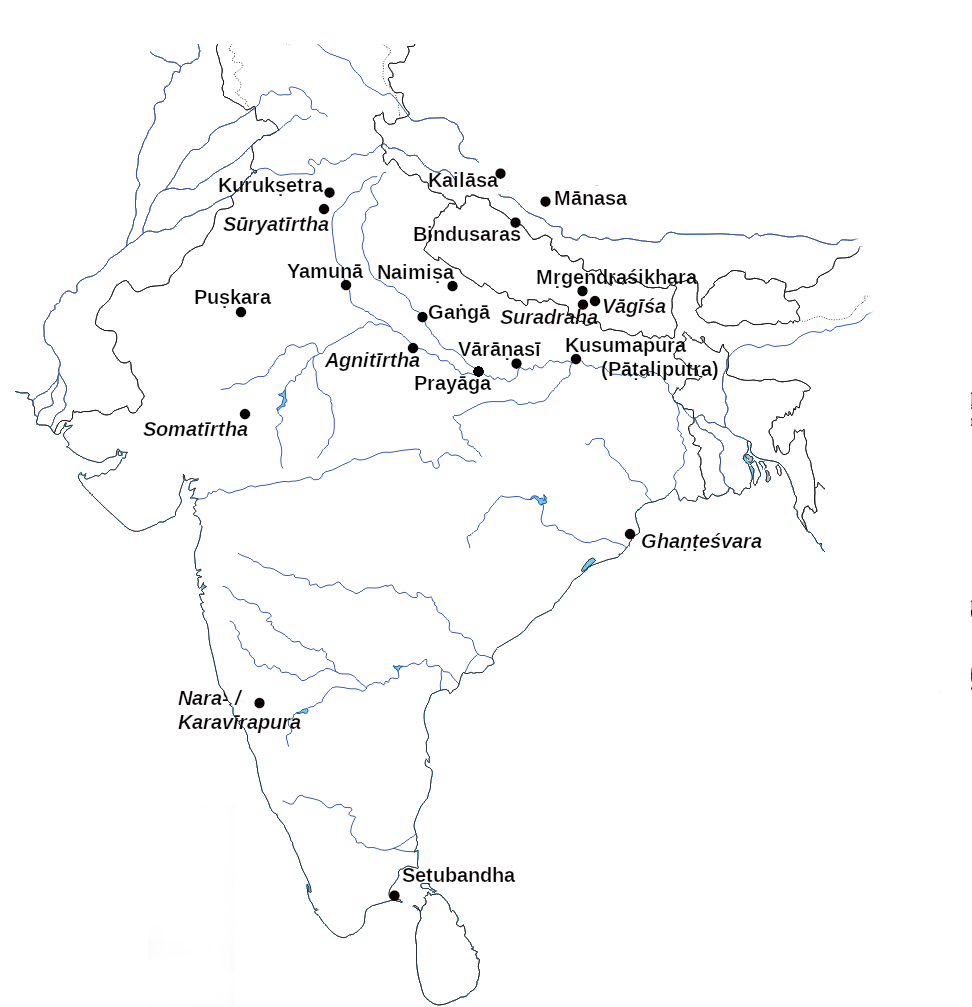
\includegraphics[scale=.35]{images/simplemap.png}
\caption[Geography of the \VSS]{A possible reconstruction of the  geography of the \VSS. Toponyms in italics are uncertain. Map constructed using a simple hydrographic map made by Daniel Dalet (d-maps.com).\label{fig:map01}}
\end{figure}

\begin{figure}[!]
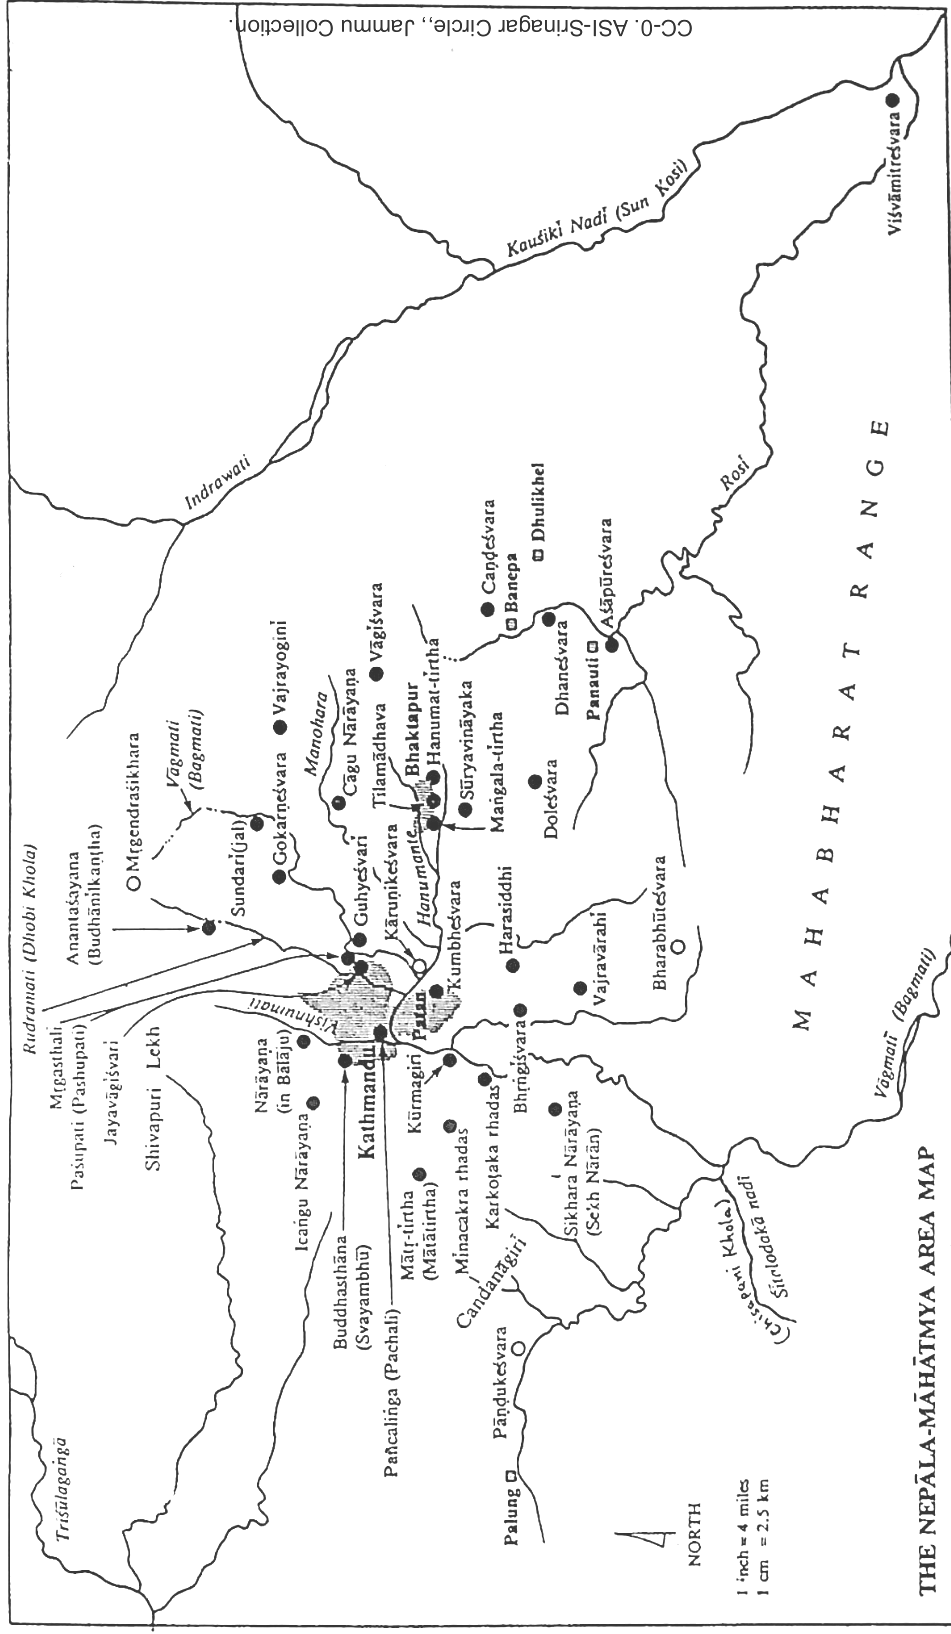
\includegraphics[scale=.40]{images/map_in_jayaraj.png}
\caption[Map in \mycite{AcharyaNepalaMahatmya}]{Map in \mycite{AcharyaNepalaMahatmya}
\label{fig:map02}}
\end{figure}


The location with which the ascetic Anarthayajña
is connected strongly suggests the Kathmandu 
valley as the geographical focus of the \VSS\
because he is a key figure and 
main interlocutor in the \VSS,
possibly the reason behind the composition of the text.%
	\footnote{On Anarthayajña's central role in the \VSS,
			see more in \mycite{KissVolume2021}.}


Turning to names of individuals mentioned in the \VSS,
those that might betray anything about the place or
time of composition of the text include King Siṃhajaṭa
and queen Kekayī, rulers of Nara- or Karavīrapura
in the narrative of chapter twelve. Unfortunately,
so far I have not been able to link these names to
any historical or legendary persons. The name of the
hero of the same chapter, Vipula,\label{Vipula} may be familiar 
from \MBH\ 13.40.16--13.43.16.: 

\begin{quote}
Devaśarman asks his disciple,
Vipula, to protect his wife, Ruci, primarily from Indra's
amorous advances, while he is away from home.
Vipula decides that the only way he can protect Ruci
is from within, i.e., by entering her body by yogic powers.
Vipula succeeds in protecting Ruci's reputation and 
departs to practise extreme austerities. Later he 
encounters several people (in fact,
as we learn later, Day and Night,
and the six seasons) who mention `Vipula's path leading to
the other world' (\skt{vipulasya pare loke yā gatis}, 
\MBH\ 13.42.27cd) as something horrible. He 
wonders what sins he may have committed that
could yield such unfortunate consequences. He
realizes that by not telling Devaśarman that he
actually entered Ruci's body, he lied and thus
may have committed a horrible sin. When Devaśarman learns
about this, he praises Vipula for his services instead, 
and all three, Devaśarman, his wife, and Vipula,
go to heaven.%
		\footnote{See a summary of Vipula's story in the 
			\MBH\ also in 
			\mycitep{SukthankarCriticalStudies}{317--318}.}
%(\MBH\ 13.43.16)
\end{quote}

\noindent
Thus, ironically, while the Vipula of the \MBH\ is famous
for protecting somebody else's wife,  
a rather different Vipula
in \VSS\ chapter twelve donates
his own wife to a Brahmin as soon as the latter expresses
interest in her. It is more than possible that
the two characters have no connection at all.%
	\footnote{Nevertheless, see the word \skt{vipule} used
	in \VSS\ 12.155b potentially referring to the famous
	story in the \MBh.}

Other characters in \VSS\ chapter twelve---Kapila, 
Vipula's father;
Bhīmabala, a traveller; Puṇḍaka, the foreman of the guild;
and Caṇḍa and Vicaṇḍa, two royal envoys---seem 
to be of little use for us to ascertain the time and place of composition or redaction of the \VSS. 

Going further, as mentioned above, any discernible influence
of a local, vernacular language on the style or grammar of
a Sanskrit work could also be useful to
locate the text in question geographically. 
The language of the \VSS\
displays numerous oddities that could be
explained by the interference of some other 
language, most likely early classical Newar.
On this, see a separate section below on 
pp.~\pageref{newar}ff.

In addition, the quotes from \Manu\ in the \VSS\
usually contain variants that can be found in the apparatus
in Olivelle's critical edition of \Manu\ (\citeyear{OlivelleManu})
as belonging overwhelmingly to
what Olivelle calls the `Northern Transmission.'%
		\footnote{See, e.g., \skt{pāpakṛt} in \VSS\ 3.34d 
		(${\approx}$\ \Manu\ 5.52) attested in Olivelle's
		Devanāgarī MSS Pu$^{5}$, Pu$^{7}$, Pu$^{9}$;
				\skt{nānyatra manur abravı̄t} in \VSS\ 3.35d 
				(${\approx}$\ \Manu\ 5.41) attested in
			Śāradā MSS {\tiny S}Ox$^{1}$, {\tiny S}Pu$^{6}$ and 
			Devanāgarī MS Tr$^{2}$;
			\skt{kūṭa} in \VSS\ 4.79 (${\approx}$ \Manu\ 11.57) in
			a MS from Kathmandu ({\tiny B}Kt$^5$), 
			in Devanāgarī/Old Nāgarī MSS
			(Lo$^{4}$, {\tiny N}Pu$^{1}$, Pu$^{2}$, Pu$^{4}$, Pu$^{10}$),
			as well as in two South-Indian MSS ({\tiny G}Md$^1$, 
			{\tiny T}Md$^3$).}
This again confirms a North-Indian or Nepalese
origin for the \VSS.

\medskip
\noindent
\label{dating}The obvious \textit{terminus ante quem} for the
composition or redaction of the \VSS\ 
is the date of the earliest MSS that transmits it.
The earliest dated MS containing the \VSS\ is \msKoa,
dated to Nepal Saṃvat 156, i.e., 1035-36 \CE.% 
	\footnote{See \mycitep{SastriCatalogue5}{721} and
		\mycitep{UmaSivaPlay}{591}. The date
	 	is clearly visible as `\skt{samvat} 156' 
	 	in the last line of the penultimate folio side 
	 	of \msKoa/8.}
In a multiple-text MS%
	\footnote{See more detail on this MS, which is
						now to be found in Munich, in	
					    \mycite{HarimotoMunichMS}.}
that is potentially earlier than \msKoa,
the \VSS\ is written in a hand that appears later than
that used for some of the other texts in that MS.%
		\footnote{\mycitep{HarimotoMunichMS}{597--598}:
		`This Śivadharma ms consists 
		of two major parts, easily distinguishable by different 		
		hands: one that appears to be produced in
		9th-c.\ Nepal [\dots], and another seemingly from 
		a century or so later [\dots] 
		The next set of folios making up this Śivadharma ms 	
		consists of three titles: the 
		\textit{Uttaromāmaheśvarasaṃvāda}* (24 folios), 
		the \textit{Vṛṣasārasaṃgraha} (50 folios), and the
		\textit{Dharmaputrikā} (11 folios). We do
		not know the original order of these three works 
		because each section starts with folio 1. Moreover, even 
		though these three titles appear to be written by the same 
		hand (probably somewhat later than the first part), there 
		is no certainty that these folios were produced to 	
		complement the first part.'}
The final colophon of the \VSS\ (and the \DHARMP) in
this MS  (\fol50r) is followed by the date
[Nepāla] `\skt{samvat} 192,' i.e., 1071-1072 \CE.

These two MSS make it impossible to date the \VSS\ later 
than the first half of the 11th century \CE, and parts of the text
may be considerably older.
Archaic features that may indicate 
that the \VSS, or parts of it, were
composed much earlier than the early 11th century
include the following. Chapter ten,%
		\footnote{Also verse 11.21.} 
while it teaches the yogic tubes
\ie{nāḍī} Suṣumnā and Iḍā, is silent on Piṅgalā, 
which is a situation similar to that in 
the 6-7-century \NisvNaya%
	\footnote{\mycitep{NisvasaGoodall}{33--35}.}  
(see details in the notes to the translation).
Similarly, 11.23a (\skt{nivṛttyādi caturvedaś}) mentions four
Śaiva \skt{kalā}s, instead of the expected and 
somewhat later, and in character tantric, five, namely
\skt{nivṛtti}, \skt{pratiṣṭhā}, \skt{vidyā}, 
\skt{śānti}, and \skt{śāntyatīta}. In the same chapter,
the order in which the \skt{āśrama}s are taught
(\skt{gṛhastha, brahmacārin, vānaprastha, parivrājaka}) 
is reminiscent of \Apastambadharmasutra\ 2.9.21.1,
and is relatively rare,
as opposed to the traditional order (\skt{brahmacārin,
gṛhastha, vānaprastha, parivrājaka}) found, e.g., in
\MANU. (See \mycitep{KissVolume2021}{195--196}.)
%cf. \mycitep{SaivaUtopia}{23}, Chapter 11, Śaiva
Another feature that might point towards a date
considerably earlier than the 11th century is the 
system of \skt{tattva}s in chapter 20:
the \skt{mahābhūta}s of classical Sāṅkhya are called 
\skt{dhātu}s here, the \skt{tanmātra}s of
classical Sāṅkhya are called \skt{guṇa}s,%
		\footnote{In contrast with, e.g.\ \SDHU\ 10.40--46 and
					\UUMS\ chapter 5, \DHARMP\ 1.42--43, or the \SIVAUP.}
the \skt{buddhi} of classical Sāṅkhya
is called \skt{mati}, and the highest \skt{tattva} 
is singular unlike the multiple \skt{puruṣa}s of classical 
Sāṅkhya. These may well be archaisms 
included in the \VSS\ consciously, but they could also
indicate that the time of composition of the \VSS\
is much closer to pre-classical Sāṅkhya than what the MS
evidence suggests.%
	\footnote{There are also numerous borrowings in \VSS\ 20
					from the Śāntiparvan of the \MBH. See more details
					at the analysis of \VSS\ chapter 20 in volume two.}

All in all, in light of all the above,
it is difficult to be more precise on the dating
of the \VSS\ than saying that its production must have
happened before the end of the 10th century, or the beginning
of the 11th century \CE\ if our oldest dated MS that transmits
the \VSS\ is close in time to the actual composition or
redaction of the text. The date could also be considerably
earlier than the 10th century, and therefore a tentative dating
for the \VSS\ would consider the 7th to 10th centuries \CE.
%    varṇas and the Liṅgapurāṇa
%    check lists of deities such as Vasus
%  bull, Nandi




% start of CGPTed section

\section{Language}\label{language}

\subsection{Newar influence?}
\label{newar}

The oddities of the language of the \VSS\ go beyond the idiosyncrasies of epic Sanskrit.
This dialect exhibits some similarities to Śaiva Aiśa Sanskrit,%
		\footnote{On Aiśa, see, e.g., \mycitep{GoodallKirana}{lxv\thinspace ff.}, 
								  \mycitep{TorzsokSYMthesis}{xxvi\thinspace ff.},
						          \mycitep{KissBraYa}{77--87}, 
						          \mycite{GerstmayrAisa}, and
						          \mycitep{HatleyBraYaVol1}{28ff.}} 
and frequently applies peculiar metrical licences, 
alongside a special vocabulary, morphology, and syntax.
Analysing this language could, ideally, help us
define the identity of the author(s) or redactor(s) of the text
and confirm our views on its place of composition.

To support a working hypothesis, I will mention parallels
between the language of the \VSS\ and early classical 
Newar---since the \VSS\ was most probably produced in the 
Kathmandu valley%
		\footnote{See pp.~\pageref{provenance}\thinspace ff.}%
---whenever possible. (This is not to suggest that the phenomena
discussed must necessarily originate in  Newar influence;
other local Prākṛts may also have played a role.)
Of course, the assumable date
of the composition of the \VSS, which is without much doubt
pre-early-11th century, does not allow any direct
comparison with contemporary Newar language texts.%
	\footnote{The earliest dated Newar document is 
			the Ukū Bāhāḥ land grant palmleaf manuscript from
			1114 \CE. See, e.g., \mycite{MallaUku}.}
Therefore I have to project a much later Newar grammar
onto an earlier and less well-known 
state of the language, which is not without risks.

In the following, I will only give a brief overview of the most
important phenomena. For details, see the observations 
on the constitution of the Sanskrit text in the footnotes 
to the translation, as well as the Index.


\subsection{Number and gender}\label{number}
One of the most evident deviation from Pāṇinian grammar in 
the text of the \VSS\ is a general disregard of grammatical concord 
in number and gender.%
	\footnote{Compare Kölver's introductory remarks in his investigation of
	`Newarized Sanskrit' (\citeyear{KolverErgative}, 202) in the \SvayP\ thus (ibid. 192):
					
					\noindent
	          	`Number is often ignored
	          	
					[\skt{catvāro 'pi maṇḍalañ ca} 429,19 (cf.\thinspace 429, 21), 
					\skt{narāḥ pañcagatiñ ca na labhec ca} 428,12],
					
					\noindent
					as is gender
					
			[\skt{tvam ekam āgataṃ na hi} 464, 10 `only you have not come’; 
			\skt{°nāgakanyā \dots\ vṛṣṭipūrṇaṃ kṛtam} 470, 8 
					`the Nāga girl made (it) full of rain'],
				
				\noindent
				and case
				
				[\skt{manuṣyāḥ \dots\ tasmai \dots\ pūjitam} 426, 2 etc. 
				`men worshipped him; he was worshipped by people'; 
				\skt{bhavatām apy arthāya karomy upāyakam mayā} 452, 5 
				`I am making an expedient for your sake'].'}
See, for example, a plural verb
(perhaps metri causa) with a singular subject in \VSS\ 1.25ab:

\begin{quote}
\skt{rātryāgame pralīyante jagat sarvaṃ carācaram} 

When [Brahmā's] night falls, the whole moving and unmoving universe dissolve[s].
\end{quote}

\noindent
Or a neuter plural participle picking up a 
neuter singular and a feminine singular noun in 1.61ab:

\begin{quote}
\skt{pramāṇaṃ nāma saṃkhyā ca kīrtitāni samāsataḥ}

The numbers [pertaining to] the measurements have been taught in brief.
\end{quote}

\noindent
Another clear example is 6.12c, where grammatical gender
is totally ignored: 

\begin{quote}
\skt{kāni lokāḥ prapadyante}

Which worlds can be attained?
\end{quote}

\noindent
Even when the \VSS\ appears to quote from the \BhG,
it tends to cause confusion for no evident reason:

\begin{quote}
        \skt{anudvegakarā vāṇī priyaṃ satyaṃ hitaṃ ca yat} (\VSS\ 6.21ab)

        \skt{anudvegakaraṃ vākyaṃ priyaṃ satyaṃ hitaṃ ca yat} (\BHG\ 17.15ab)

\end{quote}

\noindent
This line in the Bhandarkar critical edition of the \MBH\ does not 
have any significant variants, and the \VSS's version is much
more problematic grammatically than the assumable source---one can only wonder why.

This confusion---or often metrically motivated disregard---of standard Sanskrit
grammar when dealing with number and gender becomes almost
predictable when a noun phrase involves numerals.%
    \footnote{I am thankful to Judit Törzsök, who first pointed out to me
    the regular nature of the phenomenon itself as seen in the \VSS, and who 
    later drew my attention to the similar Newar grammatical rule
    (personal communication, Nov 29, 2023), which 
    led me to an investigation of a possible link between the Sanskrit of the \VSS\
    and classical Newar.}
See, e.g., verse 1.2cd:


\begin{quote}
\skt{parva cāsya śataṃ pūrṇaṃ śrutvā bhāratasaṃhitām}

Having listened to the \titleface{Mahābhārata},
to all its hundred section[s] \ie{parvan}\dots
\end{quote}

\noindent
Here, one would expect either a plural genitive \ie{parvāṇāṃ śataṃ},
a compound \ie{śataparvāṇi}, or a plural accusative \ie{parvāṇi śataṃ}.
Similarly, \skt{gatiś ca pañca vijñeyāḥ} in 3.5a stands for
\skt{gatayaś ca pañca vijñeyāḥ} (`and the paths are to be known as five'), 
partly metri causa; and an interrogative quantifier (\skt{kati}, `how many?') can
trigger the same: \skt{gatis tasya kati smṛtāḥ} (3.1d; `how many are its path[s]?').
It is worth noting that classical Newar rarely applies
any plural marker in noun phrases with numerals.\label{singularwithnumerals}% 
	\footnote{See, e.g., \mycitep{JorgensenGrammar}{18}:
			`The plural ending is wanting where plurality is expressed 
			in other ways; thus always after numerals, and
			mostly after nouns denoting ``many, all'' '.
			 Incidentally, singular after numerals is also the norm in Modern Nepali,
									 and in other, even more distant languages
									 such as Hungarian.} 
Moreover in Newar, `nouns denoting inanimate objects 
are indifferent as to number.'%
	\footnote{\mycitep{JorgensenGrammar}{5 and 17}.}
A further clear example is verse 3.6cd:

\begin{quote}
\skt{tasya patnī mahābhāgā trayodaśa sumadhyamāḥ}

       He has thirteen beautiful wives with nice waists.
\end{quote}

\noindent
Here, with no variants in any of the manuscripts consulted, only the very end 
of the noun phrase \ie{sumadhyamāḥ} bears the required 
plural ending. This again is what we often observe in Newar.%
		\footnote{`Any case [\dots] and/or plural markers [\dots], as well as 
		postpositions [\dots], are added to the last constituent of the 
		N[oun ]P[hrase].' (\mycitep{OtterCourse}{11--12}.)
		E.g.: in the Newar phrase \skt{thwo khuṃ-na khaṅ-ā rājā-pani}
		(`these kings seen by the thief'), the only indication that
		multiple kings are involved is the plural marker \skt{-pani}
		at the end (ibid.).}
A good example of total number-blindness is 5.17cd: 

\begin{quote}
\skt{kīrtitāni viśeṣeṇa śaucācāram aśeṣataḥ}

\dots\ the practice of purity is definitely expounded in great detail.
\end{quote}

\noindent
Note that there would have been little difficulty in composing the same
line in standard Sanskrit, e.g., beginning with \skt{kīrtitaṃ ca\dots}
Instead, this line betrays the author's indifference
towards grammatical concord.%
		\footnote{Compare Kölver's remark on the phrase \skt{āgataḥ sarve nāgāḥ}
		in a verse in the \SvayP\ (on p.~459 in \mycite{SastriSvayambhuP}):
		`this is a remarkable lack of sensitivity as to the category of number'
		(\mycitep{KolverErgative}{195}).}
It is also possible that the participle \skt{kīrtitāni} here
functions as a finite verb in the plural: `they teach [the practice of purity].'
In this case, there is some sense of number, but coupled with a
blurred boundary between active finite verbs and passive participles.

A special case occurs when the text appears to quote from an external source
but chooses to change the plural to the singular. E.g., \VSS\ 4.77 cites
\Manu\ 11.55, a verse that also features in the \MBH\ and in the \YAJNS.%
                \footnote{\MANU\ 11.55 (in Olivelle's edition):
                    \skt{brahmahatyā surāpānaṃ steyaṃ gurvaṅganāgamaḥ |
                         mahānti pātakāny āhuḥ saṃsargaś cāpi taiḥ saha ||};
                          \MBH\ Suppl. 12.30:
                    \skt{brahmahatyāṃ surāpānaṃ steyaṃ gurvaṅganāgamam |
                         mahānti pātakāny āhuḥ saṃyogaṃ caiva taiḥ saha ||};
                          \YAJNS\ 3.228:
                    \skt{brahmahā madyapaḥ stenas tathaiva gurutalpagaḥ |
                            ete mahāpātakino yaś ca taiḥ saha saṃvaset ||}.}
In all its versions, \skt{pāda} c of this stanza contains a plural when
labelling a list of the five `grievous sins,' except in the \VSS,
which prefers a singular.%
                \footnote{\VSS\ 4.77:
               \skt{brahmahatyā surāpānaṃ steyo gurvaṅganāgamam |
                    mahāpātakam ity āhus tatsaṃyogī ca pañcamaḥ ||}.}

There seems to be a marked tendency towards the singular in the \VSS's language. 
In general, gender confusion, and to a certain degree number confusion, are
not unusual in epic Sanskrit and in Aiśa Sanskrit,%
		\footnote{See, e.g., \mycitep{OberliesEpicSkt}{121, 292--304}, and
                \mycitep{KissBraYa}{81 and 85, and the Index therein}.}
but their extent in the \VSS\ suggests a very strong external influence---presumably
that of classical Newar.									





\subsection{Case and syntax}

An extreme example of a total disregard for Sanskrit syntax is found in \VSS~17.20:

\begin{quote}
\label{extremelanguage}
\skt{bhūmipradātā dvija hīnadīnaḥ}\\
\skt{\phantom{aaa}samṛddhasasyo jalasaṃnikṛṣṭaḥ} |\\
\skt{sa yāti lokam amarādhipasya}\\
\skt{\phantom{aaa}vimānayānena manohareṇa} ||

He who donates to a poor and distressed Brahmin land that yields plenty of corn and is in the vicinity of water will go to the world of the king of the immortal ones [i.e.\ of Indra] on a fascinating \ae rial vehicle.
\end{quote}            
            
\noindent            
Surprising as this translation may seem, it is, judging from the context, rather secure. 
\skt{Pāda}s ab probably stand for what, in more standard Sanskrit, would read:
\skt{dvijāya hīnadīnāya sasyasamṛddhāṃ jalasaṃnikṛṣṭāṃ bhūmiṃ yo dadāti}.
Instead, the phrase is constructed with what looks like a series of nominatives and a
vocative, with little or no regard for the expected case endings: endings seem to function more
as decorations than as grammatical markers.

This is difficult to explain purely in terms of Newar influence, since classical Newar does have
a dative case marker (added to the genitive for animate nouns). 
It is also striking that \skt{pāda}s cd of the same verse are composed in perfectly standard Sanskrit.%
		\footnote{See a similarly puzzling situation in the \BraYa, 
                 which is briefly described in \mycitep{KissBraYa}{74} as follows:
		`One of the most intriguing questions concerning the Bra[hma]Yā[mala] 
		is not why its language deviates from Pāṇini so often 
		but rather why sometimes it falls back to perfectly standard 
		Pāṇinian language for fairly long passages.'}

There are dozens---if not hundreds---of syntactical oddities in the \VSS,
even if not all are as baffling as the example above.%
		\footnote{Most of them are addressed in the footnotes to the translation.}
Somewhat similarly to what Kölver describes in 
his analysis of the language of the \SvayP, a Nepalese composition (\mycite{KolverErgative}),
there often (but not always) appears to be a lack of understanding of the
passive,\label{confusedpassive} 
coupled with the application of the ergative,\label{ergative} one of the
basic syntactical tools of classical Newar. 

A good example is found in 12.113cd:

\begin{quote}
\skt{indreṇāsmi phalaṃ dattaṃ sa phalaṃ datta me bhavān} 

It was Indra who gave me the fruit and I gave that fruit to you.
\end{quote}

\noindent
Again, this is the translation that seems to fit the context. 
Here the skeleton of \skt{pāda} c is a well-constructed passive:
\skt{indreṇa phalaṃ dattaṃ}, but then, instead of adding a dative or 
genitive (e.g., \skt{indreṇa me phalaṃ dattaṃ}), the author chooses 
a finite verb (\skt{asmi}). In \skt{pāda} d, after seemingly 
treating \skt{phalaṃ} as a masculine noun, and leaving
\skt{datta} in \stemform\ metri causa, and using \skt{me} for \skt{mayā},%
		\footnote{This often happens in epic Sanskrit, see 
			\mycitep{OberliesEpicSkt}{4.1.3, pp.~102--103}.}
this time he ends the phrase with a noun in the nominative \ie{bhavān} instead of
the dative or genitive. Why not write \skt{dattaṃ tad eva te mayā},%
		\footnote{Although this solution carries the metric fault of being iambic.}
or \skt{dattaṃ tava tad eva ca}?

\label{kathita}Constructions with \skt{datta}/\skt{kathita} plus an expected dative 
are especially prone to confusion. See, e.g., \VSS\ 1.62cd--63ab and 10.2d:

\begin{quote}
\skt{brahmaṇā kathitaṃ pūrṇaṃ mātariśvā yathātatham}\\
\skt{vāyunā pāda saṃkṣipya prāptaṃ cośanasaṃ purā}

        [The Purāṇas] were taught by Brahmā to 
        Mātariśvan [= Vāyu] in their entirety, in their true form.
        Vāyu abridged the verses and then gave [them] to Uśanas.
        
\skt{bravīmi vaḥ purāvṛttaṃ nandinā kathito 'smy aham}

        I shall teach you an ancient legend that Nandi told me.
\end{quote}

\noindent
Again, there is some struggle first with an expected dative here:
it ends up in the nominative \ie{mātariśvā}. Then an expected 
agent in the instrumental, or rather another dative, 
becomes an accusative \ie{uśanasaṃ}. Thirdly,
\skt{kathito 'smi} stands for \skt{kathitaṃ mama} or
\skt{kathitaṃ mahyam}. 

Somewhat similar are constructions with a 
past participle plus \skt{asmi}
in place of an active finite verb. See, e.g.,
13.68cd, 14.56ab and 15.15cd:

\begin{quote}
\skt{eṣa garbhasamutpattiḥ kathito 'smi varānane}

            This is how I have told you the formation of 
            the embryo, O Varānanā.
            
\skt{āgneyadhātuṃ somaṃ ca kathito 'smi varānane}

			I have taught, O Varānanā, the Fiery constituents 
			and the Soma-ones.
			
\skt{kathito 'smi samāsena kim anyac chrotum icchasi}

		Thus have I briefly described [to you, O Mahādevī, the soul.] 
		What else would you like to hear?
\end{quote}

\noindent
These resemble a phenomenon \citeauthor{JorgensenVicitra}
observed in a Sanskrit passage in the Newar
\VicitraKAU, where the phrase \skt{na jñāto 'ham}\label{najnatoham} must be interpreted
as `I did not know.'%
		\footnote{\mycitep{JorgensenVicitra}{77 and 328}.\label{najnatohamfn}
						Compare \skt{tat phalaṃ sa niveditaḥ} (`he gave that fruit') in \VSS\ 12:67d.}

%Vicitrakar :
%ibid and 66 \skt{aṣṭhan/au divasam āgata} should mean `Come on the eighth day'.;
%buddhamārgaṃ abhijñātaṃ: `on the well-known path of the Buddhas'
%80 and 328-329 samagraṃ, stem forms etc.!?

Occasionally, the agent of an active construction with a transitive verb
simply imitates an ergative structure: \skt{viṣṇunā\dots\ papraccha} (1.8),
\skt{dhanyās te yair idaṃ vetti} (4.75ab),
\skt{sa}[!] \skt{hovāca pathīkena} (12.60a).%
		\footnote{This happens also in Aiśa. See, e.g., \SiddhYogMata\ 18.23: 
		\skt{pūjayet \dots\ mantriṇā} (\mycitep{TorzsokSYMthesis}{42}).}
%yajec cakre ca vidhivad yoginīsiddhim icchatā 21.12cd

\label{tellplusgen}Another typical syntactical pattern in the \VSS\ is a verb
meaning `to tell, teach' followed by a noun in the genitive. See, for example, 4.69ab:

\begin{quote}
\skt{caturmaunasya vakṣyāmi śṛṇuṣvāvahito bhava}

        I shall tell you about the four cases of observing silence. 
        Listen, be attentive.
\end{quote}

\noindent
One could argue that \skt{pāda} a is simply elliptical and that
a verb like \skt{lakṣaṇaṃ} or \skt{svabhāvaṃ} 
(`the characteristics/\thinspace essence [of X]') is missing. 1.37ab and 4.17ab
display similar structures:

\begin{quote}

\skt{brahmāṇḍānāṃ prasaṃkhyātuṃ mayā śakyaṃ kathaṃ dvija}

How could I enumerate [all the details of] the Brahmāṇḍa[s], O twice-born?

\skt{evaṃ satyavidhānasya kīrtitaṃ tava suvrata}

Thus have [I] taught you the rules of truth, O virtuous one.

\end{quote}

\noindent
This phenomenon is difficult to explain as the result of Newar influence, since
classical Newar would usually also require an extra word (such as \skt{khaṃ} `thing, topic, word, story') 
in such constructions. While it may fall into one of the categories that 
Jørgensen (\citeyear{JorgensenGrammar}) describes in his \S 26 g, h, and i, 
where he gives examples of the use of the genitive,
it is more plausibly part of a broader class of phenomena that Edgerton,
in his discussion of Buddhist Hybrid Sanskrit,
labels `genitive with miscellaneous verbs.'%
		\footnote{\mycitep{EdgertonHybrid}{vol.~1, \S 7.65, p.~47}.}


These kinds of deviations from standard Sanskrit syntax require that 
the translation be, to some extent, intuitive and context-driven,
rather than mechanically adhering to the rules of standard Sanskrit grammar.%
        \footnote{Kölver's `dative for direct object'
                (\mycitep{KolverErgative}{195, 4.2.1(b)}), i.e. constructions such as 
                \skt{tasmai prapūjitam} meaning  'X worshipped him,' cannot be found in the \VSS.
                Although the \VSS\ is obviously earlier than anything Jørgensen describes,
                it may be of some interest that according to him (\citeyear{JorgensenGrammar}, \S 27b),
                this is a late phenomenon in Classical Newar.}

%end of CGPTed section

\subsection{Cardinal and ordinal numbers}

Although the \VSS\ does use simple ordinal numbers such 
as \skt{prathama}, \skt{dvi\-tī\-ya}, and \skt{tṛtīya}, with higher 
numbers there seems to be no clear distinction between cardinal and ordinal usage:
cardinals are frequently used where ordinals would be expected.
See, for example, 20.8ab and 11ab:

\begin{quote}
\skt{caturviṃśati yat{ }tattvaṃ prakṛtiṃ viddhi niścayam}\\
\skt{dvāviṃśati ahaṃkāras{ }tattvam{ }uktaṃ manīṣibhiḥ}

Know the twenty-fourth Tattva certainly as Prakṛti.
The twenty-second Tattva is Ahaṃkāra according to the wise.
\end{quote}

\noindent
This phenomenon is known, to some extent, from epic Sanskrit,%
	\footnote{See \mycitep{OberliesEpicSkt}{\S 5.2.2, pp.~127--128}.}
but is even more characteristic of classical Newar.%
		\footnote{See \mycitep{JorgensenGrammar}{42} and \mycitep{OtterCourse}{57}.}



\subsection{Stem form nouns}\label{stemform}

\Stemform\ nouns, or uninflected nominal bases (\skt{prātipadika}s), are extremely common in the
language of the \VSS. While such forms are not alien to the Aiśa Sanskrit of Śaiva Tantras,%
		\footnote{See, e.g., \mycitep{KissBraYa}{75--77} and \mycitep{NisvasaGoodall}{126 and 441}.}
the sheer frequently in the \VSS\ is striking and reminiscent one of the zero suffix of the nominative and accusative---or
rather of the `casus indefinitus' or `absolutive case'---of classical Newar.%
		\footnote{\mycitep{JorgensenGrammar}{18 and 21}, and \mycitep{OtterCourse}{16}.} 
Very often, these uninflected forms are required to restore the metre, making them difficult to emend.
Moreover, they frequently they blend in \skt{sandhi} with the following word, thus reinforcing their presence.

See some clear-cut examples, with the expected but usually unmetrical standard form in parentheses, include:

\begin{quote}
1.63a: \skt{vāyunā pāda saṃkṣipya} (\skt{pādaṃ}) \\
1.63c: \skt{tenāpi pāda saṃkṣipya} (\skt{pādaṃ}) \\
2.25c: \skt{bhogam akṣaya tatraiva} (\skt{akṣayaṃ}) \\
2.26d: \skt{īśānānāṃ smṛtālayaḥ} (\skt{smṛta ālayaḥ}) \\
4.19f: \skt{prasahyasteya pañcamam} (°\skt{steyaṃ}) \\
4.72a: \skt{caturdhyānādhunā} (°\skt{dhyānam adhunā}) \\
4.77a: \skt{pramādasthāna pañcaiva} (°\skt{sthānaṃ} or °\skt{sthānāni})
 \\
6.5c: \skt{vedādhyayana kartavyaṃ} (\skt{vedādhyayanaṃ}) \\
6.14a: \skt{dvitīyaṃ tattva puruṣaṃ} (\skt{tattvaṃ}) \\
\end{quote}




\subsection{Vocabulary}

The special vocabulary of the \VSS\ includes the following:
\skt{karhacit} for \skt{karhicit} (in some MSS in 4.3b, and 4.47b): 
        see \mycitep{EdgertonHybrid}{vol.~2, s.v. \skt{karhacid}}; 
\skt{hṛdi} as nominative 10.27cd, 20.17a, 22.24ab: 
        see \skt{diśi} in Aiśa, \mycitep{KissBraYa}{83};
\skt{tirya} for \skt{tiryañc/tiryak} (3.5c, 4.6a, 4.30a, 8.4c, 12.150,\linebreak
 18.12, 18.15, etc.);
\skt{me} instead of \skt{mayā} (8.30d, 11.4b, 12.24b, 12.55a,\linebreak
 12.113d, etc.): 
        see \mycitep{OberliesEpicSkt}{4.1.3 [pp. 102--103]};
\skt{āhūta}[\skt{saṃ}]\skt{plavana} for \skt{ā\-bhūta}[\skt{saṃ}]\skt{plavana} (2.13a, 12.151b);
\skt{puna} for \skt{punar} (1.3a): see Middle Indic \skt{puna} mentioned in
        \mycitep{EdgertonHybrid}{vol.~2, s.v. \skt{punā}}; 
\skt{nirdeha} for \skt{videha} (1.12d);
\skt{koṭya} for \skt{koṭi} (thematisation, 1.52c);
\skt{ālayana} for \skt{ālaya} (possibly 2.3a);
\skt{īrṣyatā} for \skt{īrṣyā} (2.6d);
\skt{vaṇi} for \skt{vaṇij} (thematisation, 9.16a);
\skt{sara} for \skt{saras} (thematisation, 10.27a);
\skt{sakhāyā} for \skt{sahāyā} (12.36c);
\skt{śreṣṭhi} for \skt{śreṣṭhin} (thematisation, 12.63a, 12.80a);
\skt{śaśi} for \skt{śaśin} (thematisation, 12.110d).





\subsection{Metre}\label{metre}
\label{muta}
Perhaps the most striking metrical feature of the text is its generous use of the poetic licence sometimes labelled
`muta cum liquida,'%
	\footnote{I.e. `stop with liquid.' The term `muta' stands for a `plosive' sound or `stop'. 
	 For a recent contribution on this phenomenon, see,
 	 \mycite{SenMutaCum} (discussing it as it appears in Latin).}
 	%and \mycitep{BaloghYati}??  2018, note 6 (discussing 
 	%Sanskrit metre), Balogh 2019, 39 and 115
that is, allowing a syllable to remain light \ie{laghu} 
before certain consonant clusters that would normally render it heavy \ie{guru}.%
		\footnote{On its appearance in Śaiva Tantras,
							see, e.g., \mycitep{GoodallParakhya}{lxxxi} and
							\mycitep{NisvasaGoodall}{441}. The latter concerns
							 the syllable \skt{spa} in \skt{sparśan} in \NisvNaya\ 2.55cd:
							\skt{sparśatanmātra sparśan tu gṛhṇate tvacam āśṛtaḥ}. }
Syllables beginning with \skt{pr, br, kr}, and also \skt{hr},
especially (in theory exclusively) at the beginning of words, are well-known
candidates for this licence.%
			\footnote{See, e.g., \mycitep{ApteDict}{Appendix~A p.~1}.
			Note that even here, the phenomenon extends beyond plosive sounds:
                                \skt{h} is rather a fricative.}
In the \VSS, \skt{tr, dr, bhr, vr, śr}, and also \skt{śy},%
	\footnote{See, e.g., the cadence of 5.15b: \skt{śukaśyenakān} for \ \shortsyllable\
								\shortsyllable\ - \shortsyllable\ -}
\skt{śv, sv}, and \skt{dv}, can also trigger this phenomenon.%
                        \footnote{See \mycitep{OberliesEpicSkt}{xxxvii} for an even wider
                                range of conjuncts triggering the same in the \MBH.}
All these syllables involve conjunct consonants with
a semivowel in second position. Since the sound in 
first position is not always a plosive (`muta'), the term
`muta cum liquida' is actually less than perfect in our case.
I therefore propose the terms `\krama\ licence' or '\skt{kramasaṃyoga}.' 
To give reasons for this,
% and possibly also rpa,CHECK! seem additional ones.
% Deshpande Priestly Sanskrit 421
and for context, it is perhaps not useless to briefly show
what a well-known author on prosody, 
Kedāra\-bhaṭṭa (11th or 12th century),%
		\footnote{\mycitep{OllettGana}{333}.}
who is frequently quoted by Mallinātha, has to say on this
phenomenon in his
\skttitle{Vṛttaratnākara}{Vrttaratnakara} (here given together with Sulhaṇa's
\skttitle{Sukavihṛdayanandinī}{Sukavihrdayanandini} commentary):%
		\footnote{\mycite{PatelVrttaratnakara}.}

\begin{quote}
\skt{padādāv}%
                \footnote{Some editions read \skt{pādā}°.}
\skt{iha varṇasya saṃyogaḥ kramasaṃjñikaḥ} | \\
\skt{puraḥsthitena tena syāl laghutā 'pi kvacid guroḥ} || 1.10 ||

In this [field, i.e.\ in \skt{chandaḥ\-śāstra}], conjunct consonants
\ie{saṃ\-yoga} in a word-initial syllable \ie{padādau varṇasya} is
called a `sequence' conjunct (\skt{kra\-ma}[\skt{saṃyoga}]). 
[A syllable that counts as] heavy because one
such [consonant cluster] stands in front [of it, i.e.\ after it] can 
sometimes be treated as light.

{\footnotesize [Comm.:] 
\skt{vibhaktyantaṃ padaṃ tasya padasyādau vartamāno yo varṇas tasya
saṃ\-yogaḥ} |
\skt{sa iha śāstre kramasaṃjño jñeyaḥ} |
\skt{tena krameṇa purovartinā prākpadānte vartamānasya
prāptagurubhāvasyāpi laghutā syāt} | 
\skt{kvacil lakṣ}[\skt{y}]\skt{ānu\-ro\-dhe\-na} | 
\skt{nanu ka eṣaḥ kramo nāma saṃyoga ucyate} | 
\skt{pūrvācāryāṇāṃ piṅgalanāgaprabhṛtīnāṃ kāli\-dāsādīnāṃ ca
kavīnāṃ samayaḥ parigṛhītaḥ} |
\skt{saṃyogaḥ kramasaṃyogaḥ}
||~10~||
\skt{tatra gra-saṃyogena yathā} | 
\skt{idam asyodā\-hara\-ṇam}~|

A `word' is [a unit of speach that] ends in an inflection. 
A `conjunct' is in a `syllable' which is
at the beginning of such a word. 
`In this' field of science, it is to be known under the 
term `sequence' \ie{\krama}. By that sequence which stands in front, 
[a syllable] at the end of the previous word, even if it acquired
heaviness [by position], may acquire lightness. `Sometimes' [means:]
as required.
If you have doubts about this combination of consonants called `sequence' (\krama),
[I reply:] the old teachers such as Pi\-ṅgalanāga and poets such as Kālidāsa
accepted [this] rule. The conjunct \ie{saṃyoga}
is the sequence[-type] \ie{\krama} [i.e. word-initial]
conjunct \ie{saṃyoga} [in this case].
Among [the possibilities,] for example with the conjunct \skt{gr}.
Here is an example of that:}

\skt{taruṇaṃ sarṣapaśākaṃ navaudanaṃ picchalāni ca dadhīni} |\\
\skt{alpavyayena sundari grāmyajano miṣṭam aśnāti} || 1.11 ||

Tender mustard seed, fresh porridge, and creamy curds: men in the village eat
these kinds of savoury dishes, O pretty girl, because they do not have
much money.%
	\footnote{I.e.: `you are pretty, don't waste your time with poor village men.'}
\end{quote}

\noindent
The example verse given above (1.11) is in \skt{āryā}, and the
metric pattern of the second half-verse is, strictly speaking, the following:
 
- - | \shortsyllable\ - \shortsyllable\ | - \shortsyllable\ -!~| 
- \shortsyllable\ \shortsyllable\ | 
- - | \shortsyllable\ | -  - | - |

\noindent
For any \skt{āryā}, this is unmetrical for it yields 28 mor\ae, instead
of the expected 27. By treating the final syllable of \skt{sundari} short, 
in spite of the following \skt{grā}, the pattern conforms 
to the expected pattern: 

- - | \shortsyllable\ - \shortsyllable\ | 
- \shortsyllable\ \shortsyllable\ | - \shortsyllable\ \shortsyllable\ | - - | 
\shortsyllable\ | - - | - |

\noindent
The commentator gives several more examples, involving the syllables
\skt{gra}, \skt{hra}, and \skt{bhra}, and confirms that the rule
applies only to word-initial consonant clusters: 

\begin{quote}
{\footnotesize\skt{padādāv iti kim | anyatra mā bhūt |}

Why `at the beginning of a word'? [Because] elsewhere it should not be.}
\end{quote}

\noindent
Here follow some examples from the \VSS. The syllables 
with the \krama\ conjunct consonant, before which the syllable
is not turned into heavy, are encircled, and the metre is given in 
parentheses.

\begin{quote}	
1.1c: \skt{harīndra\Circled{bra}hmādibhir āsamagraṃ} (\skt{upajāti})\\
4.67c: \skt{prajñābodha\Circled{śru}tiṃ smṛtiṃ ca labhate mānaṃ ca nityaṃ labhed} (\skt{śārdūlavikrīḍita})\\
4.89a: \skt{iti yama\Circled{pra}vibhāgaḥ kīrtito 'yaṃ dvijendra} (\skt{mālinī})\\
5.5cd: \skt{parastrīpara\Circled{dra}vyeṣu śaucaṃ kāyikam ucyate} (\skt{pathyā})\\
5.9cd: \skt{vānaprasthasya \Circled{tri}guṇaṃ yatīnāṃ tu caturguṇam}  (\skt{na-vi\-pulā})\\
5.15ab: \skt{haṃsasārasacakrāhvakukkuṭān śuka\Circled{śye}nakān} (\skt{pathyā})\\
6.13ab: \skt{brahmalokaṃ tu \Circled{pra}thamaṃ tattvaprakṛticintayā} (\skt{na-vi\-pulā})\\
8.33a: \skt{tasmān mauna\Circled{vra}taṃ sadaiva sudṛḍhaṃ kurvīta yo niścitaṃ} 
 (\skt{śārdūla\-vikrīḍita})\\
10.31b: \skt{īśānenābhijuṣṭaṃ hṛdi \Circled{hra}da vimalaṃ nādaśītāmbu\-pū\-rṇam} (\skt{srag\-dharā})\\
11.9ab: \skt{manaḥśuddhis tu \Circled{pra}thamaṃ dravyaśuddhir{ }ataḥ param} (\skt{na-vipulā})
\end{quote}

\noindent
These indeed follow the rule of having the special conjunct with the semi\-vowel
at the beginning of a word in the sense that the word can be a member
of a compound.%
		\footnote{There are some problematic verses that I ignore here. They are
						unlikely to change the overall picture.}
As noted above, since conjuncts such as \skt{śr} and \skt{hr} show up
in this phenomenon, the phrase `muta cum liquida' is slightly misleading,
and therefore I use the phrase `\krama\ licence' instead.
To understand how unique the \VSS's indulgence in this
\krama\ licence is, the epics and the Purāṇas should perhaps 
be examined from this perspective.						

\label{short2long}Another metrical oddity, or rather, metrical licence, applied
regularly in the \VSS, exclusively in non-\skt{anuṣṭubh} verses,
 is that a word-final light syllable can count 
as heavy. Here are some examples, with the light syllable now
turned heavy encircled:

\begin{quote} 

3:42d: \skt{etatpuṇyapha\Circled{la}m ahiṃsakajanaḥ prāpnoti niḥsaṃśayaḥ} 
 (\skt{śā\-rdū\-la\-vikrī\-ḍita})\\ 
 4.5a: \skt{na narmayu\Circled{kta}m anṛtaṃ hinasti} (\skt{upajāti})%
 		\footnote{Versions of this line in the \MBH\ and the \MATSP\
 								read °\skt{yuktaṃ vacanaṃ}, avoiding the metrical
								problem (see the apparatus
 								at verse 4.5 in my edition below).}\\
4.39c: \skt{aśeṣaya\Circled{jña}tapadānapuṇyaṃ}  (\skt{upajāti})\\
4.59c: \skt{vijñānadha\Circled{rma}kulakīrtināśa} (\skt{upajāti})\\
4.59d: \skt{bhavanti vi\Circled{pra} damayā vihīnāḥ} (\skt{upajāti})\\
5.20a: \skt{śaucāśaucavidhijña mānava ya\Circled{di} kālakṣaye niścayaḥ} (\skt{śā\-rdū\-la\-vikrī\-ḍita})\\
6.18b: \skt{jijñāsyantāṃ dvijen\Circled{dra} bhavadahanakaraḥ prārthanā-\linebreak ka\-lpa\-vṛkṣaḥ} (\skt{sragdharā})\\
7.13b: \skt{saubhā\Circled{gya}m atulaṃ labheta sa naro rūpaṃ tathā śobhanam} (\skt{śā\-rdū\-la\-vikrīḍita})\\
8.44d: \skt{na bhavati punaja\Circled{nma} kalpakoṭyāyute 'pi} (\skt{mālinī})\\
11.42b: \skt{saṃsāroddhara\Circled{ṇa}m anityahara\Circled{ṇa}m ajñānanirmūlanam} (\skt{śā\-rdū\-la\-vikrīḍita})\\
11.42c: \skt{prajñāvṛddhika\Circled{ra}m amoghakaraṇaṃ kleśārṇavottāraṇaṃ} (\skt{śā\-rdū\-la\-vikrīḍita})\\
11.42d: \skt{janmavyādhiha\Circled{ra}m akarmadahanaṃ sevet sa dharmo-\linebreak ttamam} (\skt{śā\-rdū\-la\-vikrīḍita})\\
12.150c: \skt{nityaṃ rogādhivā\Circled{sa}m aniyatavapuṣaṃ trāhi māṃ kāla\-pāśāt} (\skt{srag\-dharā})
\end{quote} 

\noindent
When the syllable that is turned into heavy is followed by \skt{-m}
(see 3.42d, 4.5a, 7.13b, 11.42bcd, and 12.150c among the examples above), 
the phenomenon can be treated as the one described in 
\mycitep{EdgertonHybrid}{vol.~1, \S 2.68--69, p.~19--20}:

\begin{quote}
2.68. As in M Indic generally, anusvāra is often used
instead of any final nasal. This seems to be more than a
merely orthographic matter. For it occurs before vowels,
in what must have been close juncture [\dots] 

2.69. Most texts make use of this practice in verses
for metrical convenience. It is absolutely standard practice
in all verses to use final \skt{m} before a following initial vowel
if meter requires a short final syllable, but \skt{ṃ} if a long is
required. No editor has seen this clearly; all editions are
confused and inconsistent in this respect. So are the mss.\ to 
some extent; but they follow the rule in an overwhelming
majority of instances, and there can be no question of its
original validity; the exceptions are mere corruptions of
tradition.
\end{quote}
  
\noindent
Upon re-examination, none of the witnesses of the \VSS\ that were collated, 
or only consulted for this purpose (\msCa\msCb\msCc\allowbreak\msNa\msNb\msNc\msM\msParis\msKoa\msKob),
seems to use an \skt{anusvāra} in the above cases. There is only one exception:
\msM\ writes \skt{anityaharaṇaṃ}, °\skt{vṛddhkaraṃ} 
and °\skt{vyādhiharaṃ} in 11.42 before vowels (but not
\skt{saṃsāroddharaṇaṃ}!). The same MS has neither 
\skt{ṃ} or \skt{m} in 12.150c (°\skt{vāsa aniyata}°).
One could argue that this lack of awareness of \skt{ṃ} before
a vowel indicating \skt{gurutva} in almost all cases in all MSS
are `mere corruptions of tradition,' and then typesetting
such -\skt{m} + vowel combinations as \skt{-ṃ} + vowel 
would be commendable.
On the other hand there is little evidence that in the transmission
of the \VSS\ \skt{anusvāra}s were used in this way. This is why
I hesitate to apply `Edgerton's rule' in this edition. Another argument
against applying it is all the cases in which the syllable turned into heavy
ends in a vowel (4.39c, 4.59cd, 5.20a, 6.18b, and 8.44d among the
examples above). There can be no orthographical indication of \skt{gurutva} there;
there may have not been any need of it in the other cases either.
In general, all the metrical laxity discussed above may originate from
the authors' or redactors' insensitivity to the difference between light/short and heavy/long
syllables, or short and long vowels, possibly from the underlying Newar language. 


Against Newar: no loan words no phonetic changes like l-r
%\CHECK  a more or less full collation is important: we cannot automatically reject `ungrammatical' or unmetrical forms because they may well be  the `original' one

\CHECK the more original a section the more extreme language? see ch11



\section{Authors, redactors and target audience}

It is more than likely that the \VSS\ was produced by a group 
of authors and redactors, rather than by a single individual. 
First, the extent of the text and the variety of its topics
cast doubt on whether one author could have undertaken the task.
More importantly, the language varies from chapter to chapter:
the peculiarities of the Sanskrit used in the \VSS, as described above,
do not appear to the same degree in every the chapter. 
For example, the language of chapter three display strong signs
of a possible Newar influence, and
chapter seventeen is rather problematic and non-standard,
containing some of the most ungrammatical sentences in the entire work,%
               \footnote{See p.~\pageref{extremelanguage}.}
whereas, i.e., chapter seven is relatively well-written, in a simple and 
clear style---though still far from perfect Sanskrit.

        Thus, one could picture a group of Paṇḍits---in our case, probably in 
9-10th-century Kathmandu---none of whom possessed a high degree of mastery
in Sanskrit, likely with a Newar background, and a broad knowledge
of the \MBh, the Purāṇas, Dharmaśāstra, and some limited acquaintance
with Śaiva Tantra and Buddhism.
        They might have distributed among themselves the task of writing different 
parts of the text on various topics, in an effort to create 
a new Dharmaśāstric work that introduced some radical innovations concerning the
\skt{āśrama}-system, the \skt{varṇa}s, on Śiva's world (the Śivāṇḍa), and so forth.
Surely, the different layers of the text---general Dharmaśāstric, Vaiṣṇava,
and Śaiva---were composed by authors or redactors with varying
religious and intellectual backgrounds. 
        While each individual chapter exhibits its own linguistic and compositional issues,
the final redaction---that is, the overall design of the final structure and
the assembly of the text as we now have it---is a brilliant achievement:
transitions between chapters and between doctrinal layers
are, in most cases, not only smooth but may also
encode a hidden message, suggesting a progression from the 
everyday (Dharmaśāstra) to the religious (Vaiṣṇava), 
and from the exoteric to the esoteric (Śaiva).%
        \footnote{This is not to say that there are no evident
                  contradictions and overlaps when similar teachings in different
                  chapters are compared. For instance, one teaching
                  on observing silence \ie{mauna} gives four categories
                  (4.69), while another, similar one, gives five (8.25--33).}

As for the target audience, it is difficult to say anything definite.
One of the aims of the article \mycite{KissVolume2021} was
to search for clues regarding the r\^ole of the \VSS\ in the Śivadharma corpus;
it also touches upon the possible social milieu and intended audience(s) of the \VSS.
The conclusion  therein (pp.~200--201), focusing on the fusion of 
Vaiṣṇava and Śaiva material in the \VSS, and on the reinterpretations of 
the \skt{āśrama} system in its eleventh chapter, includes the following:

\begin{quote}
The \Vss's role in the Śivadharma corpus is then twofold: 
it provides a text that is suitable for Vaiṣṇavas and Śaivas,
presenting its teachings on different levels of an esoteric scale, 
the Śaiva teachings being closest to the core, and always
providing an internalised, secret version of topics 
discussed in the other layers; and it also reinvents the traditional 
\skt{āśrama} system in a Śaiva way,
but in such a manner that would be acceptable for other religious groups. 
This may be an attempt to further develop an idea that appears in both 
the \SDhS\ and the \SDhU.%
        \footnote{[Footnote in the original:]
        These texts use new phrases for the four \skt{āśrama}s: \SDhS\
        chapter eleven uses the terms \skt{śivagṛhāśramin}, \skt{śivabrahmacārin}, 
        \skt{śivavaikhānasa} and \skt{śivavratīndra},
        while the \SDhU\ 12.203--207 uses \skt{śivabrahmacārin}, \skt{śivāśramadharmasthaḥ}
        \skt{gṛhasthaḥ}, \skt{śivāśramavanastha}, and for the fourth category both the terms \skt{pāśupata} and
        \skt{mahāvratadhara}. On this topic, see \mycitep{DeSiminiGods2016}{52--53} and 
        Bisschop, Lubin and Kafle 2021, 17 ff. [i.e., \mycitep{SaivaUtopia}{17 ff.}]}
\end{quote}

\noindent
Indeed, one of the most striking features of the \VSS\
is its structure, in which Vaiṣṇava material frames
Śaiva teachings (see pp.~\pageref{structure}\thinspace ff. above). 
Its intended audience must have included adherents of both religious traditions.
Even the title is not unambiguously Śaiva, as previously discussed
(see pp.~\pageref{title}ff. above).
Thus, we probably cannot maintain that the text is primarily Śaiva
or that its main target was lay Śaivas.
Rather, it seeks a balance between Vaiṣṇava and Śaiva teachings, 
and this duality most likely reflects the religio\-political reality of its time.

What must be stressed is the text's radicalism in certain chapters---for example, in chapters 2, 11, and 19.
These chapters appear to deconstruct the religious duties of the householder, 
internalise the social disciplines \ie{āśrama}, and reinvent 
the origin of the social classes \ie{varṇa}, respectively.
This radicalism and innovativeness may have been among the reasons for the composition of the \VSS.

A mixture of radical innovations, an idealistic rejection of the traditional \skt{varṇāśrama}-system, and the 
praise of yogic practices and the Pāśupata tradition may have been intended to
appeal both to the lay Śaiva and Vaiṣṇava householder and to aspiring yogins and ascetics.





\section{Why was the \VSS\ included in the Śivadharma corpus?}

It is difficult to ascertain why, when and how, the \VSS\ was included in the \Sivadharmacorpus.
The corpus itself, as De Simini  (\citeyear{DeSiminiMSSFromNepal2016}, 233) writes,
`as we know it seems to be an invention of Nepal'.
To summarise the relevant part of \mycite{HarimotoMunichMS} on the formation 
of the \Sivadharmacorpus, it appears that the
earliest unit formed as a collection of texts may have comprised the \SDhS\ and
the \SDhU---two texts probably composed, or at least known, outside Nepal---and the
\SDhSangr, whose provenance remains obscure.
These were later joined by the \UMS, and then by the beginning of the tenth century \CE, 
by the \SivaUp.
This development is inferred from some of the colophons in the Munich MS (MS \msM):
the colophon of the \UMS, the fourth text in that MS---likely copied from an earlier exemplar---suggests
that the corpus was considered fourfold, whereas the colophon of the \SivaUp,
the fifth text, presents it as fivefold (\mycitep{HarimotoMunichMS}{600--603}).
In MS \msM, the \VSS\ appears to have been written in a later hand, perhaps
indicating that it was added subsequently.


The \VSS\ may have already been existence, most probably in the Kathmandu valley,
well before the beginning of the tenth century (see p.~\pageref{provenance}ff).
It was probably added to the collection after the original set of three or four
texts had been augmented with additional texts in Nepal. The \VSS\ must have been considered
a valuable work, and its survival was secured by its attachment to a 
prestigious corpus. Alternatively, it may have been commissioned by a king in Kathmandu
after a preliminary version of the corpus had already become well-known, 
in response to a perceived need to add a locally composed text.





%%% CG start %%%
\section{Contents of chapters 1--12}\label{contentsof1_12}

The following are brief descriptions of the topics covered in chapters 
1--12 of the \VSS, which have been edited and translated in this volume. 
These are accompanied by brief discussions and some analytical remarks.%	
		\footnote{See more details in the footnotes to the translation.
                          See a Sanskrit summary of the contents of the \VSS, based on Naraharinath's edition,
                          in \mycitep{AnilkumarBook}{61--72}. }

					
\subsection*{Adhyāya 1}\label{contents_of_ch01}
After a \skt{maṅgala}-verse that addresses a 
deity whose identity is obscure\linebreak
(verse 1.1; is it Śiva or the 
impersonal Brahman?), we enter the first layer 
of the text, which consists of a dialogue between Janamejaya and 
Vaiśampāyana. This layer could be labelled Dharmaśāstric.
Janamejaya seeks to hear the essence---the ultimate Dharmic 
teaching---of the \MBh. In response, Vaiśampāyana begins relating 
a dialogue in which Viṣṇu, disguised as a Brahmin, 
tests an ascetic named Anarthayajña, renowned for performing 
non-material, i.e., internalised, sacrifice (\skt{anarthayajña}, 
the subject of \skt{adhyāya} eleven), and 
a devotee of Viṣṇu (as revealed in \skt{adhyāya} twenty-one). 
This marks the beginning of the layer that could be labelled Vaiṣṇava (see pp.~\pageref{structure}ff). 

The first topic they discuss is \skt{brahmavidyā} (1.9--10), an
ambiguous definition of the impersonal Brahman and/or the syllable \skt{oṃ}. 
The next topics include \skt{kāla} (`death, time'), the origin of the body, karma (1.11--17), 
and the divisions of time (from \skt{truṭi} and \skt{nimeṣa} up to \skt{kalpa}s, 1.18--30), 
which lead to a teaching on numbers, ranging from one up to 
two hundred quadrillion (\skt{para}, 1.31--35).
Verses 1.36--39 introduce a list of the rulers of the eight 
regions of Brahmā's Egg (Brahmāṇḍa, that is, the universe, 1.40--48). 
In addition, Viṣṇu is presented as the ruler of the centre of the Brahmāṇḍa (1.49),  
reaffirming the general Vaiṣṇava character of this layer. 
Verses 1.50--57 give the numbers of subordinates to each ruler mentioned above. 
Verses 1.58--61 teach the measurements of the Brahmāṇḍa. 
Finally, verses 1.62--75 list the redactors and transmitters of the Purāṇas, 
from Brahmā to Vyāsa Dvaipāyana, Romaharṣa, and Romaharṣa's son Amitabuddhi.


% Keywords: Brahmā, Brahman
%
% 11:35:18 From somadeva vasudeva To Everyone : There is a very relevant forthcoming study by H. Kondo: “Fault Lines of Samkya History: Struggling with the Conflict between Satkarayvada and the Accumulation Theory” where he analyses exactly the differing accounts of the exact role of the tanmatras, using also Chinese sources. Hopefully our Journal will be able to publish it this year.
%11:40:18 From somadeva vasudeva To Everyone : Kenji can tell you more, but for dating also consider the Carakasamhita’s “samkhya section”.
%12:02:18 From Yuko Yokochi To Everyone : Three grāmas are in the Nāṭyaśāstra.
%12:03:10 From somadeva vasudeva To Everyone : Check maybe also the B.rhadde”sii of Matas”nga
%12:03:16 From Sathyanarayana Sarma To Csaba Kiss(Privately) : Sorry Csaba, I had other reading, so I couldn’t join.
%12:04:55 From serenasaccone To Everyone : Thanks for the talk and lively discussion! Have to go. See you soon!
%12:11:38 From Csaba Kiss To Sathyanarayana Sarma(Privately) : https://filedn.com/lFSw9FGgUBpyrpsGtImyUHh/textprocess_javascript.html
%12:12:05 From Csaba Kiss To Sathyanarayana Sarma(Privately) : (Another approach at the above link.)

 
\subsection*{Adhyāya 2}\label{contents_of_ch02}
Seemingly a reaction, counterpart, or addendum to the previous chapter which
discussed Brahmā's Egg, this chapter introduces Śiva's Egg (Śivā\-ṇḍa),
potentially an innovation of the \VSS. Śiva's Egg is portrayed as an esoteric, mysterious, and
thus superior part of the universe, accessible only through 
Śaiva yogic practices (\skt{śiva\-yoga}, 2.34). A description is given of
an idealistic and egalitarian society (`There is no master or servant there, 
nobody to be punished and no punisher,' etc., 2.5ff). The text goes on 
to deconstruct the `Hindu' religious universe and the Dharmic ritual 
life of the devotee, eliminating the Kalpas and \skt{karma} (2.11--12), 
all mythological creatures (2.14--15), and ritual action (2.16).

Following this, the text describes the details of the Śivāṇḍa---its 
height and width, its lovely flowers, fruits, golden trees, 
gem trees, coral gem thickets and ruby plants (2.17--25). 
The chapter then introduces a scheme that divides the Śivāṇḍa 
into five regions, each connected to one of Śiva's five faces, and
subdivided into the thirty-eight \skt{kalā}s of the five Brahmamantras.

This chapter can be perceived as an innovative attempt to reinforce the
Śaiva character of the text, counterbalancing the previous chapter.
It also seems to reflect tantric, or pre-tantric, Pāśupata ideas and 
further emphasises the text's yogic character by implementing 
another esoteric, meditative layer of the universe above, or outside
the Brahmāṇḍa (\skt{śivāṇḍābhyantareṇaiva}, 1.39a). One could theorise that
this chapter is a tantric, or Pāśupata, insertion in a non-tantric text, 
but the fact that the Śivāṇḍa was already mentioned in chapter 
one suggests that the two chapters were likely composed at the same time.
 
Overall, the concept of the Śivāṇḍa appears to be
a bold attempt to transcend the fundamentals of \skt{varṇāśramadharma}
in a radical manner by relativising basic social and moral distinctions.
This perhaps distantly echoes Pāśupata teachings, and suggests that Śaivism---or
perhaps tantric Śaivism---is superior to generic Dharmaśāstric tenets. This radicalism,
perhaps the main motive behind the composition of the \VSS, is perceivable
again in chapter eleven, which discusses the internalisation of the \skt{āśrama}-system, and 
in chapter nineteen, where it is suggested that the \skt{varṇa}s originate from a social contract.
 



\subsection*{Adhyāya 3}\label{contents_of_ch03}

This chapter starts with general questions about Dharma,
including the etymology of the word \skt{dharma}, 
Dharma's embodiments---especially as a bull---and 
the family of personified Dharma (3.1--13).
Dharma is declared to be the embodiment of Śruti and Smṛti (3.14--15).
Smṛti is described as concerning the \skt{varṇāśrama}-system, as well as 
rules of conduct, i.e., the \skt{yama} and \skt{niyama} rules, which are the
focus of 3.16--8.44. Each rule is five-fold.
The \skt{yama}s are: \skt{ahiṃsā, satya, asteya, ānṛśaṃsya, dama, ghṛṇā,
dhanya, apramāda, mādhurya}, and \skt{ārjava}. This list is more similar to
ones found in the \MBh\ than to yogic lists such as the one in the
\YogaS,%
		\footnote{See, e.g., \MBh\ 12.8.17ab: 
						\skt{ahiṃsā satyavacanam ānṛśaṃsyaṃ damo ghṛṇā}.
						On \skt{yama}s and \skt{niyama}s in the \SDHS\ and related
					   texts, see also \mycite{SaivaUtopia}{11--17}.}
but the closest parallel is found in the \VDhU.% 
%śaucam ijyā tapo dānaṃ svādhyāyopasthanigrahaḥ ||
%vratopavāso maunaṃ ca snānaṃ ca niyamā daśa ||202 ||
		\footnote{\VDHU\ 3.233.203:
				\skt{ānṛśaṃsyaṃ kṣamā satyam ahiṃsā ca damaḥ spṛhā} |
				\skt{dhyānaṃ prasādo mādhuryaṃ cārjavaṃ ca yamā daśa} ||.
						The \VDhU\ is probably earlier than 1000 \CE\ (see 
						\mycitep{RocherPuranas1986}{252}).}

The rest of this chapter elaborates on the first \skt{yama}, 
non-violence (\skt{a\-hiṃsā}), focusing particularly on the five kinds of violence (3.18--23).
After a general praise of non-violence (3.24--32), the text discusses restrictions
on meat consumption, quoting \Manu\ in 3.34--37.


\subsection*{Adhyāya 4}\label{contents_of_ch04}
Verses 4.1--17 discuss the second \skt{yama}, truthfulness (\skt{satya}). 
After defining truth (\skt{satya}, 4.1), rules for speaking the truth are presented,
illustrated with references to mythological stories. 

Verses 4.18--30 cover the third 
\skt{yama}, refraining from stealing (\skt{asteya}). 
The fourth \skt{yama}, absence of hostility (\skt{ānṛśaṃsya}), is 
introduced in verses 4.31--49. It consists of being kind to Śiva, 
to fathers and mothers, cows, and guests,
with particular emphasis on the praise of cows and rules of hospitality.  
The story of the mongoose in the \MBH\ (\MBH\ 14.92--93)
is mentioned in this context.

Verses 4.50--59 elaborate on the fifth \skt{yama},
self-restraint (\skt{dama}), possibly drawing on the 
\Buddhacarita,  with further references to mythological stories.
The sixth \skt{yama}, concerning taboos (\skt{ghṛṇā}) is addressed in verses 4.60--67.
These taboos concern restrictions on sexual partners, taking away others' wealth and
lives, hurting others, and commensality.

The seventh \skt{yama} is \skt{dhanya}, which I translate as `virtue' (4.68--76).
Five areas of practising virtue are mentioned here: 
maintaining silence in four situations;
conquering the fourfold enemy---desire, anger, greed, and delusion;
the `four sanctuaries' (\skt{caturāyatana}), which are in fact the
Buddhist \skt{brahmavihāra}s; four types of meditation (on \skt{ātman, vidyā,}
Śiva, and the Subtle One); and Dharma as a four-legged bull. The
basic pattern is that each of its five subcategories has a fourfold structure.

The eighth \skt{yama} provides instructions how to avoid mistakes and committing sins
(\skt{apramāda}, 4.77--82), with verses 4.77--81 following \Manu.
The ninth \skt{yama} is charm (\skt{mādhurya}), which involves being kind both mentally
and through bodily actions (4.83--85). 
The tenth and final \skt{yama} is sincerity (\skt{ārjava}, 4.86--89),
completing the section on the ten \skt{yama}s.



\subsection*{Adhyāya 5}\label{contents_of_ch05}

This chapter begins the section on the \skt{niyama} rules, which are
\skt{śauca, ijyā, tapas, dāna, svādhyāya, upasthanigraha,
vrata, upavāsa, mauna,} and\linebreak \skt{snāna}. This list also appears in the
\LinPu\ (1.8.29cd--30ab) and the \VDhU\ (3.233.202).
The discussion on the first \skt{niyama}, purity (\skt{śauca}, 5.4--20) seems
incomplete. As usual, we expect a list of five sub-types, 
but there seem to be only four here. The third and fourth types
(\skt{mātrā}- and \skt{bhāva-śauca}) are rather vague, and 
no details are given about them. 
While the first two---bodily purity and purity of food---are 
discussed to some extent, partly drawing on \Manu\ in verses 5.5--9 and 5.10--16, 
the rest of the discussion is quite general. It seems likely that
the author of this section borrowed a list of four or five items from 
an external source but felt unable to elaborate on some of them.




\subsection*{Adhyāya 6}\label{contents_of_ch06}
The second \skt{niyama}, sacrifice (\skt{ijyā}), is discussed in verses
6.1--18. It again includes five types: material sacrifice, sacrifice through
work and through recitation, knowledge, and meditation. Corresponding
or similar teachings on the `five \skt{mahāyajña}s' can be found in texts
such as the \BhG\ (4.28), \Manu\ (3.69--71), and \SDhU\ (1.10).
The section on sacrifice through meditation \ie{dhyānayajña} 
describes visualisations that lead one to 
Brahmaloka, Viṣṇuloka, Śivaloka, etc., if practised at the 
time of dying. The visualisations themselves are
reminiscent of some of the teachings in the \DharmP.%
        \footnote{See p.~\pageref{dhyanayajna}.}

The third \skt{niyama}, penance (\skt{tapas}) is the focus of verses 6.19--28.
with verses 6.21--22 echoing the \MBh.


\subsection*{Adhyāya 7}\label{contents_of_ch07}
This chapter addresses the fourth \skt{niyama}, donation (\skt{dāna}).
The five subcategories here are donation of food, clothes, gold, land, and cows
(7.1--25). The chapter concludes with praise for the practice of donation (7.26--28).

This chapter is relatively well-written, composed in simple and generally
straightforward language, in contrast to some passages in the previous
chapters that contain radically non-standard Sanskrit. One cannot help feeling that the
author or redactor of this and some of the following chapters is different
from those of chapters one and two, for example.



\subsection*{Adhyāya 8}\label{contents_of_ch08}
In a similarly more or less straightforward chapter, six additional 
\skt{niyama} rules are taught. The fifth \skt{niyama}, study (\skt{svādhyāya}) 
is covered first (8.1--6). The five pillars of the intellectual
milieu in which this teaching was likely composed are
Śaivism, Sāṃkhya philosophy, the Purāṇas, Smārta texts (i.e., Dharmaśāstra),
and the \MBh\ (8.1). Śaivism is defined through the dichotomy of the Śaiva and Pāśupata
traditions. The Sāṃkhya-\skt{tattva}s are said to be taught in groups of five,
suggesting a 25-\skt{tattva} system. The \MBh\ is identified as \skt{itihāsa}. 

Verses 8.7--12 list the five types of sexual offences that constitute
the sixth \skt{niyama} rule (\skt{upasthanigraha}).

Verses 8.13--18 address the seventh \skt{niyama}, religious
observances (\skt{vra\-ta}). Four of these observances are, in principle, 
imitations of animal behaviour: cats, herons, dogs, and cows. The fifth is
somewhat obscure but could be an imitation of Bhīṣma's dying scene in the \MBh.
All of these observances are radical and may be based on Pāśupata practices.

Verses 8.19--24 teach dietary restrictions as the eighth \skt{niyama} rule (\skt{upavāsa}),
with verse 8.21 drawing on the \MBh.
Verses 8.25--33 describe the ninth \skt{niyama}, \skt{mauna}, outlining
when to remain silent and what to avoid saying, including abusive speech and insults.

Ritual bathing (\skt{snāna}) concludes the chapter in verses 8.34--44. This 
tenth \skt{niyama} rule, and consists of five types: fire-bath, water-bath, Vedic bath,
Wind bath, and divine or heavenly bath.  

This chapter also concludes the entire section, which has
taught twenty major rules in total, each theoretically consisting of five subcategories.




\subsection*{Adhyāya 9}\label{contents_of_ch09}
This chapter turns to a discussion of the three Guṇas, \skt{sattva, rajas,} and \skt{tamas}.
The treatment of the topic seems less philosophical and more moralising and classificatory.
It categorizes gods, people, animals, plants, activities, and foods into Sāttvika, Rājasa, 
and Tāmasa, as well as into superior, mediocre, and low variants of Sāttvika, Rājasa, etc.
Mixed categories such as Tāmasa-Rājasa are also mentioned. 

The chapter concludes by introducing the yogic or moral concept of a state of being 
beyond the Guṇas (9.39--43), again most probably inspired by the \MBH.

\subsection*{Adhyāya 10}\label{contents_of_ch10}
At the very beginning of this chapter, our interlocutors, Vigatarāga and Anarthayajña,
hand over the narration to Nandikeśvara, who immediately begins recounting
a dialogue between Śiva and Devī. This marks a shift to a new layer of the text,
which can be labelled Śaiva. The topic discussed is internalised pilgrimage places (\skt{tīrtha}).

The significance of this chapter lies in the possibility that the topographical
names mentioned, and their hierarchy, may provide clues about the text's
place of composition. Another clue---this time for the dating of the text---is that,
while the yogic tubes Suṣumnā and Iḍā are mentioned in verses 10.17 and 20--21,
there is no clear mention of Piṅgalā, the third tube traditionally associated with them,
anywhere in the text. For more details on both topics, see pp.~\pageref{provenance}ff.

\subsection*{Adhyāya 11}\label{contents_of_ch11}
This chapter is crucial for understanding what the \VSS\ may have aspired to achieve and 
why the main interlocutor of the Vaiṣṇava chapters is named Anartayajña. The primary
focus here is `non-material' sacrifice, or \skt{an\-artha\-yajña}, which essentially
represents internalized sacrifice or worship, or rather the internalisation of all aspects of
the religious life of a `Hindu' devotee, within each of the four social disciplines (\skt{āśrama}).

Given the omnipresence of the name and concept of Anarthayajña/\skt{an\-artha\-yajña}, 
this chapter could be central to the development of the entire text. 
See pp.~\pageref{nonmaterial}ff and \mycite{KissVolume2021} for more details.
 

\subsection*{Adhyāya 12}\label{contents_of_ch12}
Although non-violence is mentioned alongside hospitality as a
topic to be discussed in this chapter, it is clear that hospitality 
is the primary focus of this long chapter.
Following verse 12.3, we find a charming, fairy-tale-like narrative
about the adventures of Vipula, a merchant of Pāṭaliputra. 
Vipula is forced to give his wife to a visiting 
Brahmin to honour his promise to his guest, 
which leads him to leave his home and wander southward.
At this point a series of miraculous events unfolds,
triggered by the fact that a magical fruit with the power of bestowing 
youthfulness is gifted to him by a monkey. Instead of eating the fruit,
Vipula gives it away, and the king of Naravīrapura (i.e., Karavīrapura?)
orders him to obtain more such fruits. 

A quest for more fruit leads Vipula to the Gandharva king, god Sūrya, Soma, Indra, Viṣṇu, and
ultimately to Brahmā's palace.

The story ends abruptly, giving the impression that it was
part of a longer narrative. Although the story's starting point
is the necessity to satisfy a guest's wishes (\skt{ātithya}, or 
the rules of guest reception), another key focus appears to 
be the rewards of donation or gifting (\skt{dāna}): Vipula gifts his wife to the Brahmin;
a monkey gives him a magical fruit; he gives the magical fruit to the foreman of the guild;
the foreman gives the fruit to the king; 
it turns out that the fruit was originally given to the monkey by the Gandharva king; 
who in turn received it from Indra; and so forth. 
    
One of the lessons suggested by the story’s conclusion---where
Vipula is honored by Brahmā and other gods---is
that donors eventually receive great rewards. 
The narrative also features a recurring theme of testing people while in disguise: 
Viṣṇu tests Anarthayajña disguised as Vigatarāga (see 1.7–8), 
and now Vipula seems to be tested by a Brahmin who may in fact be Dharma himself (12.37).

\section{Topics in chapters 13--24}\label{contentsof12_24}
Here follow some preliminary summaries of the chapters in the second half of the text, to be edited and translated in volume two.

\subsection*{Adhyāya 13}\label{contents_of_ch13}
After possibly referring back to chapters ten, eleven, and twelve, Devī now asks Mahādeva
what purpose the easy method (\skt{sukhopāya}) serves when people and divine beings remain indifferent.
Mahādeva's reply contains references to the three \skt{guṇa}s and this prompts another question from Devī about them. 

The reply that follows touches upon the three Sāṃkhya categories \skt{prākṛta}-, \skt{vaikṛta}-, and \skt{dakṣiṇābandha}---and
transmigration (13.1--14). This triggers another question about the formation of the embryo \ie{garbhotpatti}.
The rest of this chapter deals with this topic, as well as the pain of being reborn (13.15--68).

\subsection*{Adhyāya 14}\label{contents_of_ch14}
A continuation of the previous chapter, this one deals with the question of differences in bodily appearance 
among humans: why are some people short or fat, others tall or thin? Mahādeva explains that food consumed
and actions taken during pregnancy are the main causes (14.1--5). Devī's next question concerns bodily defects in 
a child, such as blindness, lameness, being born hump-backed or as a dwarf. Again, it is the pregnant woman who is
to blame (14.6--29). 

Then the reasons why a child is born male, female, or gender-neutral \ie{apuṃs} are given:
it depends on the proportion in which the male semen and the female blood (14.30--32) mix.
The production of semen is discussed (14.33--38),
as well as the possibility of remembering past lives (14.39--40),
and the signs of pregnancy and the signs whether a boy or a girl has been conceived (14.40--46). 

The production of bodily hair is then discussed (14.47--52), alongside the topic of \skt{somadhātu} and \skt{agnidhātu}
(14.47--56).

\subsection*{Adhyāya 15}\label{contents_of_ch15}
The first section of this chapter deals with the characteristics of the soul (\skt{jīvalakṣaṇa}, 15.1--15).
Then, prompted by Devī's request, Mahādeva provides a list of what constitutes the best within various categories:
the best of the four \skt{āśrama}s, the four \skt{varṇa}s, sacrifices, recitations,
deities, rivers, and so on (15.16--29).

\subsection*{Adhyāya 16}\label{contents_of_ch16}
This chapter discusses yogic practices. The introduction (16.1--13) contains some verses that parallel
various texts: a citation in Kauṇḍinya's commentary on the \titleface{Pāśupatasūtra}\index{Pasupatasutra@\textit{Pāśupata\-sūtra}},
the \MBh, the \BhavP, and the \AgniP.

The next section (16.14--18) is more specific about yogic techniques \ie{yogavidhi}: 
eight sitting postures are listed (\skt{padmaka, svastika, niṣkala, añjali, ardhacandra, daṇḍa, paryaṅka, bhadra}),
and a \skt{ṣaḍaṅga}-type yogic system is explicitly introduced (\skt{pratyāhāra, dhyāna, prāṇāyāma, dhāraṇā, tarka, samādhi}).

From verse 18 onwards we find a series of verses that have close parallels in the \DharmP\ (16.18--29). The signs of 
successful practice are enumerated (16.30--32). Verses 16.33--35 give hints on liberation without yogic practice.

Next (16.33--47), a new topic is introduced, namely the five important branches of knowledge \ie{śāstra}:
Sāṃkhya, Yoga, the Pañcarātra, the Śaiva revelation, and Vedic knowledge (echoing and altering \MBh\ 12.336.1).
Devī expresses her satisfaction with what she has heard (16.48--50) and asks Maheśvara to continue
and teach her about donations \ie{dāna}.


\subsection*{Adhyāya 17}\label{contents_of_ch17}
The topics in the first part of this chapter are as follows: the donation of food, clothes, land, cows, gold (17.1--25).
This is followed by miscellaneous verses connected to donations and the corresponding rewards that manifest in the next life (17.26--33).

Next come some verses alluding to Purāṇic stories about donation (17.34--36), and the topic of donating one's own flesh and blood,
son and wife (17.37--52), again citing legends from the \MBh\ and the Purāṇas. 

The chapter ends by a brief discussion of the levels of donation (17.53--57) and their respective rewards.


\subsection*{Adhyāya 18}\label{contents_of_ch18}
The main topic in this chapter is the marks that indicate that a man
has been to heaven or hell before being reborn in his present life.
For example, if somebody regularly gave food to the poor, he will
depart to Īśaloka and, in his next life, will be rich. 
Alternatively, if one kills a Brahmin, one goes to hell,
will spend millions of years as an animal and then will
be reborn as a diseased and poor man.

Several examples of this sort are given throughout the chapter. 

\subsection*{Adhyāya 19}\label{contents_of_ch19}
Verses 19.1--19 deal with the importance and sacredness of the cow.
Then the origin of the social classes \ie{varṇa} is discussed, stating
that originally there was only one \skt{varṇa},%
                \footnote{\skt{ekavarṇo dvijaś cāsīt sarvakalpāgram agrataḥ} (19:21).
                `Before the very beginning of all \ae ons, 
                 there was one single class of Brahmins.'}
and it was only later that the four classes developed driven by the need to
distribute tasks (19.20--36).

Next, the types of penance, worship, and sacred places 
connected with the individual \skt{varṇa}s are listed.


\subsection*{Adhyāya 20}\label{contents_of_ch20}
This chapter deals with a \MBh-type 25-\skt{tattva} ontological system,
as opposed to a Classical Sāṃkhya-type teaching: no \skt{tanmātra}s are mentioned,
instead the term \skt{guṇa} is used; instead of \skt{mahābhūta}s, \skt{dhātu}s
are presented. Also, \skt{buddhi} is called \skt{mati}, and the 25th \skt{tattva}
is simultaneously Śiva, Brahmā, and the Puruṣa.

Verses 20.23--32 deal with the \skt{prāṇa}s. 
Verses 20.83--89 discuss the state of \skt{unmanastva}.


\subsection*{Adhyāya 21}\label{contents_of_ch21}
In this chapter Viṣṇu reveals his real form to Anarthayajña, who 
has not been aware that the Brahmin Vigatarāga, whom he has been 
teaching is in fact Viṣṇu in disguise. Anarthayajña praises Viṣṇu,
who, being satisfied, takes him by the hand and leads him to Viṣṇuloka.

By this we are brought back to the outermost layer of the text:
the dialogue between Janamejaya and Vaiśampāyana.
The topic here is the \ae ons \ie{kalpa}.

\subsection*{Adhyāya 22}\label{contents_of_ch22}
Here Janamejaya enquires about Anarthayajña.
In reply, Vaiśampāyana gives details about Anarthayajña's dwelling place,%
                \footnote{See pp.~\pageref{anarthayajnas_asrama}ff.}
and religious practice called \skt{anarthayajña}, described in more detail in chapter eleven. 

Yogic practices that echo chapter sixteen are described.
A cryptic ten-syllable mantra is presented in an encoded form, followed by
verses on religious conduct \ie{ācāra}, women, and various categories of
professionals of religious practice \ie{vipra, muni, bhikṣu, nirgranthi, parivrājaka, rṣi}.

\subsection*{Adhyāya 23}\label{contents_of_ch23}
Janamejaya asks Vaiśampāyana about the reason why gods and demons fight. 
This leads to a discussion on \skt{dharma} and \skt{adharma}, and on good and bad conduct.
This is followed by verses on how sleep arises.

\subsection*{Adhyāya 24}\label{contents_of_ch24}
Janamejaya wishes to hear about the divisions of the world and the heavens: the hells \ie{naraka}),
the netherworld \ie{pātāla}, the seven islands \ie{dvīpa}, Śivaloka, and so on.

The text ends with praise of the \skt{sāstra} itself and with the enumeration of the rewards
that one receives if one reads, recites, or listens to this text.

\vfill
\pagebreak


%% end of passage checked with CGPT







%%%%%%%%%%%%%%%%%%%%
% CRITICAL EDITION %
%%%%%%%%%%%%%%%%%%%% 
% to add vertical space in the TOC
%\addtocontents{toc}{\protect\vspace{20pt}}

\mychapter{Introduction to the Critical Edition}
\section{Preliminary remarks}

%While it is probably unnecessary to argue in favour of
%producing a high-quality edition of any of the texts in the Śivadharma
%corpus---given its importance for our understanding
%of the history of Śaivism---
It is perhaps worth clarifying why the versions of the \VSS\ and other texts of
the Śivadharma corpus as printed in \mycite{NaraharinathSivadharma} are not satisfactory,%
		\footnote{As \citeauthor{WestTextual} (\citeyear{WestTextual}, 61) 
			puts it, following a long tradition of philologists:
			`Is your edition really necessary? That is the first question.'}
and why there is a need to produce high-quality critical editions of them.
One could simply refer the reader to the apparatus in
this new edition: the readings given in \citeauthor{NaraharinathSivadharma}'s 
\emph{editio princeps} rarely prove useful or are 
accepted against the manuscript evidence.
One could also point out further problems in 
\citeauthor{NaraharinathSivadharma}'s edition, such
as countless typos, misreadings, and readings and omissions that 
may come from his law-quality sources,%
		\footnote{Just to quote a few from the first few verses:
								\skt{sahasrādhyāyar uttamam} for \skt{sahasrādhyāyam uttamam} (1.2b),
								\skt{nāradasaṃhitāṃ} for \skt{bhāratasaṃhitām} (1.2d),
								\skt{śaṃkha} for \skt{śaṅkuḥ} (1.34b), omissions in 1.34cd--35, etc.}
and a lack of any critical apparatus or any documentation of the witness(es) used.%
		\footnote{He must have worked from paper manuscripts,
								see p.~\pageref{narahari_paperms}.}
In addition to this, although it does not affect this volume,
a great chunk of the text, \VSS\ 17.38--18.16, is
missing in \citeauthor{NaraharinathSivadharma}.

It would be more difficult than this to vindicate in detail the methology
I have applied. I find \citeauthor{HannederIntro}'s 
words on textual criticism comforting:

\begin{quote}
[T]extual criticism is often viewed as something to be learned by practice rather from reading about it.
\dots\ In fact, both translating and editing are something most Indologists have learned in a pragmatic
way through examples from within the field, and some have managed to become quite good at it.
\dots\ [I]n most cases this approach is sufficient \dots%
		\footnote{\mycitep{HannederIntro}{5}.}
\end{quote}

\noindent
My experience is that when preparing critical editions, each text, 
and sometimes each manuscript or each chapter, \textit{horribile dictu},
each verse, requires a slightly different approach, and these approaches 
keep changing during the editorial process. For example, the idea that 
there could be a connection between the linguistic oddities of 
the \VSS\ and classical Newar
%		\footnote{See p.~\pageref{newar}.}
arose relatively late, and it did change my views on some textual
problems and some of the solutions thereof, and led me to change some
of my previously proposed emendations.
Thus editing is always subjective in the sense that the method
applied is influenced by the editor's knowledge of the text, the genre,
the milieu, etc., or in the case of this edition, the collective knowledge
of all my colleagues who took part in \VSS\ reading session and brain-storming
meetings throughout the years.

Since it is not unlikely that originally the \VSS\ had multiple authors and redactors,
the text itself is also unlikely to be homogenous: each chapter may
have its own style and its own types of textual problems. In addition 
to this, all MSS we have access to surely trasmit a highly contaminated
version of the text. This makes the construction of a stemma codicum more or less
useless in this case.


\bigskip

\section{Witnesses}

\fancyhead[CE]{{\footnotesize \textit{Vṛṣasārasaṃgraha}}}
\fancyhead[CO]{{\footnotesize \textit{Witnesses}}}
\fancyhead[LE]{}
\fancyhead[RE]{}
\fancyhead[LO]{}
\fancyhead[RO]{}

\noindent
In the pre-modern era, the \VSS\ has been transmitted exclusively in multiple-text manuscripts that were produced in Nepal. Even when a
manuscript of the \VSS\ seems to be a single-text MS, 
chances are high that it originally belonged to a multiple-text
manuscript.%
	\footnote{\label{noteonKolkataMs}As I remarked elsewhere 
	(\mycitep{KissVolume2021}{185, n.~9}):
	`Asiatic Society (Calcutta), Manuscript G 4076, cat. no. 4083, 
	may seem to be an independent manuscript of the 
	\textit{Vṛṣasārasaṃgraha}, but as De Simini has already 
	remarked (2016b, 240 n. 19),  % [= \mycite{DeSiminiMSSFromNepal2016}],
	it is probably from a multiple text manuscript. In fact, from what
	can be gathered from its description in
	\mycitep{SastriCatalogue5}{716ff},
	it seems likely that this manuscript was
	originally part of manuscript Asiatic Society (Calcutta) G 3852, cat.\
	no.\ 4085. See for example the folio numbering in these two 
	manuscripts: ASC G 3852 contains 210 folios, 
	and ASC G 4076 starts on folio 210.'}
In the manuscript descriptions below, in addition to some general
remarks, I will mainly focus on information relevant to the \VSS. For
much more detail on the overall features of these manuscripts, see 
\mycite{DeSiminiMSSFromNepal2016}, \mycite{BisschopUniversal}, 
\mycite{SaivaUtopia}, \mycite{SDhS10_ed},  
and the catalogues I mention
at some of the individual manuscript.%
		\footnote{I owe thanks to Florinda De Simini for 
			sharing with me most of the manuscripts listed here, to
  			Kengo Harimoto and Gudrun Melzer (Munich) for 
  			providing photos of the  Munich MS, and to 
  			Nirajan Kafle for sharing a digital 
  			copy of the Paris MS with me.}

In recently published and forthcoming critical editions of and articles
on the Śivadharma corpus,%
		 \footnote{\mycite{BisschopUniversal}, 
						\mycite{SaivaUtopia}, and \mycite{SDhS10_ed}.}
the sigla of the manuscripts used are made up of 
a letter signifying the script (e.g.~`N' for
Nepālākṣara/Newari), a superscript letter for the current location where
the manuscript is deposited (e.g.~`C' for Cambridge), 
and two (sometimes only one or even three) subscript 
digits echoing the last digit(s), if any, of the reference 
number of the manuscript in the 
library where it is located or, in the case of NGMPP reel 
numbers, the last two digits of the first part of the reel number.%
			\footnote{For details of this system and for the underlying reasons, see 
								\mycitep{BisschopUniversal}{50--51}.}
Since in the case of the \VSS\ all the 
manuscripts I utilised are written in
some variant of the Nepālākṣara script,%
		\footnote{I have not used NGMCP B 219/3 
		NAK 4/2537 (paper, Maithilī script), and \msL\
		(paper, Devanāgarī script, see below).} 
in this publication I omit the first letter, 
making the letter for the current location non-superscript. 
This helps keeping the apparatus readable. 
In the manuscript descriptions below, I give this 
omitted and implied `N' in brackets as a reminder.

Note that I mention here not only those MSS collated 
for the whole or parts of the critical edition, but also some 
that were initially considered for collation but later completely dismissed. 
I have retained the readings of a MS in the apparatus 
even if that MS was collated only for part of the text.
To justify this practice, I refer to \mycitep{NisvasaGoodall}{103}, 
which describes a similar approach towards abandoned witnesses.%
                \footnote{`[MS] T [\dots] proved to be of such poor quality that we abandoned
        including its readings after collating just three chapters, \textit{Nayasūtra} 2--4.
        We have left most of its readings in the apparatus so that some data is available
        that shows how poor it is, but we have not collated it for the \textit{Mūlasūtra} and
        \textit{Uttarasūtra}.'}

%\section{How to describe a MS?}\label{how-to-describe-a-ms}

%In general these categories should be included: - {[}X{]} Siglum - {[} {]} Location where it is deposited - {[} {]} Ms no. - {[} {]} How much do I use it? - {[} {]} Catalogued by and where and under what no., with what title - {[} {]} what does the catalogue says - {[} {]} Physical: - {[} {]} material - {[} {]} dimensions - {[} {]} no of folios - {[} {]} condition - {[} {]} format, binding - {[} {]} Text - {[} {]} script - {[} {]} contains these texts - {[} {]} complete - {[} {]} language (implied) - {[} {]} MTM? - {[} {]} foliation - {[} {]} hands - {[} {]} initial rubric, incipit, explicit, final rubric (in edition) - {[} {]} colophons (in edition) - {[} {]} dating - {[} {]} description in detail, remarks

\label{msssigla}
\medskip
\label{mss_descr}
\subsection{Cambridge manuscripts}

\msdescr{(N)\msCa}{nc94}
Cambridge University Library, Add. 1694.1. This MS has been 
fully collated for chapters 1--12 of the critical edition in this volume. 
See a detailed description of this manuscript in the 
CUDL online catalogue.\footnote{https://cudl.lib.cam.ac.uk/view/MS-ADD-01694-00001/382}
According to this catalogue, the date of creation of this manuscript 
is the 12th century, and its dimensions are 5~×~ca.\thinspace 53.5 cm. 
The script is Nepālākṣara. It is a palm-leaf multiple-text manuscript containing 258
folios and transmitting eight texts: 
1)~\SDhS,
2)~\SDhU,
3)~\SDhSangr,
4)~\Ums,
5)~\Uums, 
6)~\Vss,
7)~\DharmP,
8)~\SivaUp.

The \VSS\ occupies 45 folios: it starts on \fol193v. 
The recto side, online image no.\thinspace381, is an empty folio side. 
The text ends on \fol239r (online image no.\thinspace473). 
The text of the \VSS\ is transmitted fully,
without any folios or major sections of the text missing. The leaves
transmitting the \VSS\ are well-preserved. Some folio sides are faded and
most folios are somewhat damaged on the right side, 
sometimes at other parts, and it seems from the images 
that some opaque-looking tape has been applied to protect these damaged sections. 
In my critical edition the broken off, completely lost, 
\emph{akṣara}s are represented by \lac,
the illegible \emph{akṣara}s under the tape by \lk\ (`illegible'). The
quality of the readings of this manuscript is one of the best among
the available witnesses, comparable only to \msNa\ and \msParis, 
making it one of the most important sources for the \VSS.


\msdescr{(N)\msCb}{nc45}
Cambridge University Library, Add. 1645. This MS has been fully
collated for chapters 1--12 of the critical edition in this volume. 
See a detailed description of this manuscript in the CUDL online catalogue.\footnote{https://cudl.lib.cam.ac.uk/view/MS-ADD-01645/404}
According to this catalogue, its dimensions are 
4.4~×~61.7~cm. The manu\-script is dated to (Nepāla) `\emph{samvat} 259
\emph{śrāvaṇa śukla dvādaśiyā di} \textless{} \emph{trayodaśyām},'
which converts to July 10/11 Monday/Tuesday, 1139 \CE.%
		 \footnote{\Fol247r line 6. The CUDL website transcribes this
		  colophon as: \skt{saṃvat} 259 
		  \skt{śrāvaṇaśukladvādaśi{\rm[}pyaḍi} 8 
		  \skt{trayodaśyāṃ} (retrived 8 Dec 2021). 
		  The element \skt{dvādaśipyaḍi} could be read as
		  \skt{dvādaśiyā di}, perhaps a mistake for
		   \skt{dvādaśyāṃ}
		  \skt{di} (\skt{di} for a misplaced \skt{diva/divā}?), and the
		  symbol that does look like a figure `8' of a slightly later period
		  than the manuscript itself (resembling the mathematical symbol
		  \textless{}) might also be a \skt{kākapada}. 
		  Alternatively, one could understand \skt{yā} as a Newar genitive marker,
		  \skt{dvādaśi-yā di} meaning `the day of the twelfth.'
		  Another faint
		  \skt{kākapada} is perhaps to be seen under \skt{daśi},
		  therefore it is possible that the scribe's intention was to delete 	
		  \skt{dvādaśi} and correct it to \skt{trayodaśyām}, 
		  and then the date becomes 11th of July.
		  Kengo Harimoto 
		  has suggested that the unclear element
		  (\skt{yādi/pyaḍi}) is in fact \skt{ghaṭi}, 
		  and after comparing these two syllables to other instances of
		  \skt{gha} and \skt{ṭa}, one cannot but agree. 
		  In this case this should be an indication of the
		  exact time (Skt. \skt{ghaṭi/ghaṭikā}, Newar \skt{ghaṭi}) 
		  the scribe finished copying the text. It is still not clear
		  if we should take \skt{dvādaśi} or \skt{trayodaśyām} 
		  as the date. For help on the conversion of the date and 
		  for a detailed discussion on the colophon I am indebted
		  to Kengo Harimoto.} 
The script is Nepālā\-kṣara. It is a palm-leaf multiple-text 
manuscript containing 247 folios. Eight texts are transmitted 
in this manuscript: 
1)~\SDhS,
2)~\SDhU,
3)~\SDhSangr,
4)~\SivaUp,
5)~\Ums,
6)~\Uums, 
7)~\Vss,
8)~\DharmP.


The \VSS\ occupies 37 folios plus one folio side: it starts on \fol201v
line 4 (online image no.\thinspace 404), 
and it ends on \fol238v line 3 (online image
no.\thinspace 478). 
The readings of this manuscript seem to follow those of \msNa\
remarkably closely while transmitting the 
Śivadharmottara (as observed by De Simini and Harimoto).%
\footnote{Personal communication, 1 Dec 2021.} This
is more difficult to see in the case of the \VSS, 
but indeed, they seem closely related. 
%CHECK MORE on this


\msdescr{(N)\msCc}{nc02}
Cambridge University Library, Add.\thinspace 2102. 
All available folios of this MS have been collated for 
chapters 1--12 of the critical edition in this volume. 
See a detailed description of this manuscript 
in the CUDL online catalogue.%
	\footnote{https://cudl.lib.cam.ac.uk/view/MS-ADD-02102/181}
According to this catalogue, the date of creation is the 12th
century, and the dimensions of the manuscript are 
4.8~×~ca.\thinspace 52.5~cm. 
The script is Nepālākṣara. It is a palm-leaf multiple-text manuscript
containing 96 folios. Six texts are transmitted in this manuscript: 
1)~\SDhU,
2)~\SDhSangr,
3)~\Ums,
4)~\SivaUp,
5)~\Vss,
6)~\DharmP\ (only \fol322v). 
Note that the \SDhU\ starts on \fol51r, thus the part that most probably contained the \SDhS\ is lost.

The \VSS\ starts on \fol267r line 1 
(online image no.\thinspace181). 
The online description labels this image as \fol237r. 
This first folio in fact has no visible foliation.
The previous text, the \SivaUp,
ended on \fol236v, with pāda b of verse 7.122,%
 		\footnote{Image no.\thinspace180, 
                  \SivaUp\ 7.122: \skt{yauvanasthā gṛhasthāś ca}
                  {[}\skt{prāsā}{]}\skt{dasthāś ca ye nṛpāḥ}.}
which is not the end of the \SivaUp: 
about eighteen verses, probably transmitted 
in one single folio, are lost.
This means that, if the foliation and the order of the folios
are presented correctly, and if the portion containing
the \VSS\ indeed belongs to the same manuscript, 
folios 237--266, i.e.\ thirty folios, are missing. 
They must have transmitted the \Uums, 
which takes up twenty-three folios in \msCa, and twenty folios in \msCb.
Thus this MS did most probably transmit all eight texts of the
Śivadharma corpus.%
	\footnote{Compare with the claim of the online catalogue:
		``The present manuscript probably contained seven texts.''}	

This first folio of the \VSS\ is in a hand which is different from the
rest of the manuscript, but the hand changes back in the next folio.\label{msCcfirstfolio}%
	\footnote{Cf.~the metadata on the CUDL site: 
	`1 folio of the same dimensions is a modern supply for the 
	beginning of the \skt{Vṛṣasārasaṃgraha}.' A hardly readable 
	note in pencil to the same effect is visible at the
    top of the first folio side (\fol267r, `mode\ldots\ldots 
    supply beg of Vṛṣasāra-saṃgr.'). I am not sure how `modern'   
    this supplement is, but it seems indeed likely that a lost 
    first folio was supplemented
    with a later copy. To match the end of this new copy with the
   beginning of the next, older, folio, a scribe more or less erased   
   the beginning of the first line in the old folio, 
   rather than the last line
   of the younger folio. 
   This slightly illogical decision may mean that the younger
   copy was not tailor-made for the old portion, 
   but rather that it was
   taken from a younger manuscript which was 
   perhaps considered more legible. 
   Otherwise it would have been more practical to stop copying
   the first folio at the point where the next begins.
   See some more detail on this folio on
    p.~\pageref{msCcfirstfoliokakapada} below.}




In this multiple-text manuscript, the \VSS\ is transmitted in an incomplete
form, that is to say, a number of folios are missing (most notably
chapters 15--17). The first partially visible folio number is in image
184: the numeral characters 200+60 are visible (268v, according to the
CUDL online catalogue). In image 186, the folio number 269 is clearly
visible (\fol269v). On folio 270v, the continuous text is interrupted at verse
2.21c (\skt{kāmarū°}), \fols271 and 272 are missing, and the text
resumes on \fol273r with verse 3.30b ({[}\skt{ahiṃsā
pa}{]}\skt{ramaṃ} \skt{sukham}). Folio 291 is missing (verses
12.87cd--12.113). On folio 296v (image no. 234), the text breaks off
again at \skt{vātaśūlair upadrutā} | \skt{śukro} (at verse 14.22b),%
        \footnote{Of course, my verse numbering in chapters 13--24 may change slightly
                  during the editing process.}
the next folio being 306r (starting with \skt{carmatāś ca dvijasundarīṣu},
verse 18.27b; nine folios, including chapters 15 to 17, are missing entirely).

Again, there are two missing folios after \skt{bandhus sarvva°} in
verse 18.47c on \fol306v. The text resumes on \fol309r (image 237)
with \skt{°ṇeṣu ca sarvveṣu vidvān sreṣṭha sa ucyate} (verse 19.52cd). 
Another folio is missing between \skt{iṣṭāniṣṭadvaya°} (verse
20.22, \fol309v) and \skt{snāyu majjā sirā tathā} (verse 20.51d, \fol311r). The \VSS\ ends on \fol322v (image no.\thinspace262) with the
concluding colophon \skt{vṛṣasārasaṅgraha samāpta iti}. 
This folio also contains the beginning of the \skt{Dharmaputrikā}, 
but this multiple-text manuscript contains no more folios.

In the apparatus, the siglum \mssCaCbCc\ signifies all three Cambridge 
MSS described above.

\medskip
\subsection{Kathmandu palm-leaf manuscripts}
\msdescr{(N)\msNa}{nk82}
NGMPP A 1082/3, NAK 3/393. This MS has been fully 
collated for chapters 1--12 of the critical edition in this volume. 
See a brief description of this MS in
the NGMCP online catalogue.%
	\footnote{https://catalogue.ngmcp.uni-hamburg.de/receive/aaingmcp\_ngmcpdocument\_00098499}
According to this catalogue, the dimensions of the 
manuscript are 55.6 × 5.5 cm. 
It is dated to Nepāla Samvat 189 (1068--69 \CE).%
	\footnote{See \fol12r line 2 of the 
	\DharmP\ in this MS: 
	\emph{navottarāsītiyute sate bde āsāḍhaśuklasya
  tithau tṛtīye}, translated by \mycitep{DeSiminiMSSFromNepal2016}{252 n.\thinspace 49} as: 
  `in {[}the year{]} 189, in the 3rd lunar day of the bright {[}fortnight{]}
  of {[}the month{]} Āṣāḍha.' She adds that the date is verified in
  Petech 1984, 46 as May 24, 1069 \CE.} The script is Nepālākṣara and it is
a palm-leaf multiple-text manuscript containing 274 folios. Eight texts
are transmitted in this manuscript: 
1)~\SDhS,
2)~\SDhU,
3)~\SDhSangr,
4)~\Ums,
5)~\SivaUp,
6)~\Vss,
7)~\DharmP,
8)~\Uums.

As for each text in this collection, the foliation for the
\VSS\ restarts from \fol1v (\fol1r is a cover) and the text
spans \fols1v--46r. This is a beautifully written and well-preserved
manuscript which gives accurate, or at least useful, readings and has proved to be
essential for the reconstruction of the \VSS.%
	\footnote{See a similar evaluation in
					\mycitep{BisschopUniversal}{56}.}


\msdescr{(N)\msNb}{nk10}
NGMPP A 10/5, NAK 1/1261. This MS has been fully collated 
for chapters 1--12 of the critical edition in this volume. 
See a brief description of this MS in
the NGMCP online catalogue.\footnote{https://catalogue.ngmcp.uni-hamburg.de/receive/aaingmcp\_ngmcpdocument\_00085264}
According to this catalogue, the dimensions of the manuscript are 55 x
5.5 cm. It is an undated palm-leaf multiple-text manuscript containing 74
folios. Four texts are transmitted in this manuscript: 
1)~\SDhU,
2)~\Ums,
3)~\SivaUp,
4)~\Vss.

Some folios feature drawings. 
A great number of the leaves that 
transmit the \VSS\ are damaged and, 
at least judging from the microfilm images, 
faded and slightly disordered. The folio numbers are
rarely visible. The \VSS\ starts on exp.\thinspace 44 
(upper leaf, no folio number is visible here). 
The text continues on the lower leaf and then on the upper
leaf on exp.\thinspace43 (going backwards, so to say) 
up to 1.60 (\skt{viṃśakoṭiṣu gulmeṣu ūrdhva°}). 
Verses 1.60d--2.22 seem to be missing. The lower leaf on
exp.\thinspace43 contains verses 2.23--2.39. 
The single leaf in exp.\thinspace42 contains
verses 2.40--3.16a. Exp.\thinspace41 contains a single leaf of the
\skt{Umāmaheśvarasaṃvāda}, ending in a colophon for its chapter
twenty-two, and still going backwards, the preceding folios continue
transmitting the 
\Ums. 
Exploring the presence of
the \VSS\ in this manuscript further, 
one should look at the expositions
after no.\thinspace44. Exp.\thinspace45 contains the end of the
\SivaUp. The
single leaf on exp.\thinspace46 
is almost illegible but most probably contains a fragment of the \GautDhS. 
The second line just above the string hole on the left reads \skt{\ldots{} vīrud vanaspatīnāṃ ca
puṣpāṇi svavad} \skt{ādadīte\ldots{}}, which is a fragment of \GautDhS\ 2.3.25 (12.28). 
The remaining parts of the \VSS\ are to be found on exp.\thinspace47ff. 
The upper leaf on exp.\thinspace47 continues with
\VSS\ 3.16b--36ab, while the lower leaf contains a text that I have not
been able to identify. The lower leaf in exp.\thinspace48 transmits
3.36cd--4.11ab, the upper one 4.11b--30a. The lower leaf in 
exp.\thinspace49 contains 4.30ab--47ab, 
the upper one 47d--68a, and so on so forth. Thus
when reading the text from these images, after exp.\thinspace48, 
one has to start with the lower leaf and continue with the upper one.


\msdescr{(N)\msNc}{nk7}
NGMPP B 7/3 = A 1082/2, NAK 1/1075. This MS has been 
fully collated for chapters 1--12 of
the critical edition in this volume. See a brief description of this MS
in the NGMCP online catalogue.\footnote{https://catalogue.ngmcp.uni-hamburg.de/receive/aaingmcp\_ngmcpdocument\_00062373}
According to this catalogue, the dimensions of the manuscript are 
58 × 6 cm. The script is Nepālākṣara. Dated to Nepāla Samvat 
290 (1169--70 \CE). It is a
palm-leaf multiple-text manuscript containing 289 folios. Eight texts
are transmitted in this manuscript: 
1)~\SDhS,
2)~\SDhU,
3)~\SDhSangr,
4)~\Ums,
5)~\SivaUp,
6)~\Vss,
7)~\Uums,
8)~\DharmP.
\Fols209v--264v contain the \VSS.

This is a nicely written manuscript, giving generally useful and
convincing readings. 


\msdescr{(N)\msNd}{nk3}
NGMPP A 3/3 (= A 1081/5), NAK 5-737. I have collated 
this MS only for verses 1.1--15ab to test it. 
See a brief description of this MS in the NGMCP online
catalogue.%
	\footnote{http://catalogue-old.ngmcp.uni-hamburg.de/mediawiki/index.php/A\_3-3\_Śivadharma} 
According to this catalogue, the dimensions of the manuscript are
58.5 x 5.5 cm. The script is Nepālākṣara and the MS is dated 
to Nepāla Samvat 321 (1200--01 \CE). It is a palm-leaf multiple-text manuscript containing 215 folios.
Eight texts are transmitted in this manuscript: 
1)~\SDhS,
2)~\SDhU,
3)~\SDhSangr\ (only a few folios are extant, e.g. \fols124 and 143), 
4)~\Ums,
5)~\SivaUp,
6)~\Uums,
7)~\Vss,
8)~\DharmP.

The \VSS\ begins on \fol227 (image no.\thinspace177) 
and appears to conclude after starting chapter 23 
on \fol264 (image no.\thinspace 218). However, the last image 
(no.\thinspace253) still contains a fragment of \VSS\ chapter 13.
The microfilm images are somewhat blurred, 
making it difficult to confidently decipher the text,
and the readings do not seem promising.


\bigskip

\noindent
Other palm-leaf MSS preserved in Kathmandu, but not used for
this critical edition include the following:

NGMPP A 11/3, NAK 5--738% 
%Palm-leaf, dated to NS 516 (1395--96 CE), 253 folios. Contents: Śivadharmaśāstra (fols.~1v--43r); Śivadharmottara (fols.~4v--95r); Śivadharmasaṃgraha (fols.~96v--139v); Umāmaheśvarasaṃvāda (fols.~140v-- 171r); Śivopaniṣad (fols.~172v--189r); Uttarottaramahāsaṃvāda (fols.~190v-- 211v); Vṛṣasārasaṃgraha(fols.~212v--257v). For a description of this manuscript, also see the record in the NGMCP online catalogue: \textless{}
	\footnote{http://catalogue.ngmcp.uni-hamburg.de/wiki/A\_11- 3\_Śivadharmottara}%
---the microfilm images of the folios containing the \VSS\ are often blurred to an extent that makes them
difficult to use.


NGMPP C 25/1, Kesar Library 218---this multiple-text manuscript
preserves only a few misarranged folios of the \VSS.
%Palm-leaf, 298 folios.
%Contents: Śivadharmaśāstra (fols.~1v--57r); Śivadharmottara (fols.57v--134v); Śivadharmasaṃgraha (fols.~135r--215v); Umāmaheśvarasaṃvāda (fols.~216v--255r); Śivopaniṣad (fols. 256v--278r); Umottara°/ Uttarottaramahāsaṃvāda (fols. 279v--299v¤); Vṛṣasārasaṃgraha (?¤--?¤); (?--?¤).

\medskip
\subsection{Paris manuscript}

\msdescr{(N)\msParis}{np57}
This is a multiple-text palm-leaf manuscript written in 
Nepālā\-kṣara script and preserved in the 
Collection Sylvain Lévi at the Institut d'études
indiennes, Collège de France as MS Skt 57-B 23. 
I have collated the readings of this MS for \VSS\ 
chapters one (available only up 1.58a), 
chapter two (available only from 2.19c),
three (available only up to 3.14),
and eight. % and 17
It contains 249 palm leaves. % each folio containing six lines. 
Folios 214 and 216 are missing from the 
part of the manuscript that transmits the \VSS,
thus we do not have verses 1.58d--2.21ab, as well as
3.14--4.7. In addition, verses 12.152--16.19 and 17.51--18.20ab are missing.
%also 3, 8, 47, 48, 135, 197, .
%Folio 215v ends with \skt{kautūhalam atī} in 3.14a and the next available folio starts with \skt{tyam iṣṭagatiḥ proktaṃ} in 4.8a. This means that verses 3.14--42 and 4.1--7 of the VSS, altogether 36 verses are missing. This is indeed approximately the number of verses that two folio sides contain.
Foliation appears on the verso side: in the left-hand margin in
Newar alphabetical numerals and in the right-hand margin 
in arabic numerals by a second hand. 
%There are two binding holes: one in the centre
%left and one in the centre right. 
The portion that contains the \VSS\ is relatively well-preserved and
the text is written in a clear hand. Although it is an undated manuscript,
it could be dated to the 11th century \CE\ on 
pal{\ae}ographical grounds. 
It contains the following text in the order they are presented in the manuscript:
1)~\SDhS, % (\fols1--40), 
2)~\SDhU, % (\fols40--93), 
3)~\SDhSangr, % (\fols94--142), 
4)~\Ums, % (\fols143--172), 
5)~\SivaUp, % (\fols173-- 189), 
6)~\Uums, % (\fols190--211), 
7)~\Vss, % (\fols212--252), 
8)~\DharmP. %(\fols253--262). 
The \VSS\ appears on \fols212--252.
This source gives reliable readings and contains
relatively few scribal mistakes.%
	\footnote{This description had as its starting 
	point a shorter description written and kindly shared with me by Nirajan Kafle.}
Note that \msParis\ seems to be closely related to \msKOb; see remarks
on this at the description of \msKOb\ below.
%Śivāśramādhyāya covers fols.~33v4--37r3. Nirajan says it reads close to Naraharinātha's edition




\medskip
\subsection{Munich manuscript}

\msdescr{\msM}{munichMS}
This MS is preserved at the Ludwig Maximilian University
in\linebreak \mbox{Munich}, Germany.%
			\footnote{\mycitep{HarimotoMunichMS}{596}. 
			See more detail in that paper.}
It has no access number.
I have collated the readings of this MS only for \VSS\ 
chapters one and five as a test. % and ch. 18
I received the digital images of this MS from Kengo Harimoto
shortly after he had taken pictures of it in Munich on  Nov 16, 2021. 
This MS contains the following texts:
1)~\SDhS, 
2)~\SDhU, 
3)~\Ums,
4)~\SivaUp,
5)~\Vss, 
6)~\Uums,
7)~\DharmP.
The section that must have contained the \SDhSangr, \fols82--121, is lost. 
The portion that contains the \VSS\ and the \DharmP\
is dated (\fol50r line 5): \skt{|| iti vṛṣasārasaṅgrahe caturviṃśatimo dhyāyaḥ samāptaḥ | samvat} 192 \skt{māghakṛṣṇadivāpañcamyām || postakalikhitam iti ||.} The year 192 in Nepāla Samvat converts to 
1071--1072 \CE. The part of the MS the precedes the \VSS\ looks
considerably earlier and is potentially an important witness for
other texts of the Śivadharma corpus. An interesting 
feature of this MS is that it gives the number of verses contained in
each chapter in the colophons. Ten folios that transmitted the \VSS\
are missing: 
\fol5 (\VSS\ 3.4-3.33),
\fols11--13 (\VSS\ 6.20--8.45),
\fols24 (\VSS\ 13.9--13.36), and
\fols39--43 (\VSS\ 20.38--22.35). 
%*416.jpg lower image is Dharmaputrikā 4.22-39)
%  417.jpg upper is Dharmaputrikā 4.39-55
%The \VSS\ starts in 411.jpg `cover' {[}411.jpg{]}: ||w||vṛṣasārasaṃgraha 50 patra ||w|| Text starts in 412.jpeg, f.1r Ends on image 455.jpeg 
% Kengo writes: ``411.jpg forms a cover that says vṛṣasārasaṅgraha but it is actually 50 verso'' samvat 282? {[}that would be 1161 CE, or is it 292? = 1171 CE{]} No, maybe 192! see Kengo's notes! = 1070 CE

The foliation for the \VSS\ restarts
and the hand in which the \VSS\ and the \DharmP\ are written are different from, and
most probably later than that of the texts that come 
before them in this bundle. 

The MS often transmits unique and interesting readings
but rarely convincing ones, and in general does not seem to be superior 
to any of the MSS described above. But at some points
I did follow its reading against the other witnesses, e.g., at 5.1b.








\medskip
\subsection{Kolkata manuscripts}



%I have not been able to access either of these two potentially important witnesses:



\msdescr{(N)\msKOa}{nko77}
%According to \mycitep{shastri_descriptive_1928}{720},
MS G4077 in the collection of the Asiatic Society, Kolkata.%
	\footnote{I am grateful to Daniella Cappello and Marco Francheschini
                  for managing to obtain digital copies of some of the folios of this MS.
                  At the moment I have the folios that contain 1.1--11.59ab.}
This MS contains the following texts:
1)~\SDhS, 
2)~\SDhU, 
3)~\SDhSangr,
4)~\Ums,
5)~\SivaUp,
6)~\Uums,
7)~\Vss, 
8)~\Lalita.%
        \footnote{See \mycitep{SastriCatalogue5}{718--723}.}
The \VSS\ is transmitted in 52 folios; foliation restarts from f.~1.
The MS is dated to July 6, 1036 \CE\ (Nepāla Samvat 156; 
see \mycitep{DeSiminiLachmann2017}{542}), which makes
it `the oldest known dated attestation of the corpus'
(\mycitep{DeSiminiMSSFromNepal2016}{250--251}).
Nevertheless, after collating it for verses 1.1--16 and 8.1--8,
I abandoned it, since its readings offered little of value and,
if anything, added considerable noise and clutter to the apparatus.%
        \footnote{Another random sample to show the low quality of this source
                  would be f.~19v, line 3--4 (compare with verses 11.55--56 in 
                  the edition):
                  \skt{vigatarāgaṃ tu dhanuḥ kṛtvā prāṇāyāmaguṇair{ }yutam} |
                  \skt{dhāraṇāsaratīkṣṇena mṛgaṃ ḍhatvā manendriyaṃ} ||
                  \skt{maitrīkhaḍgam atīkṣṇena saṃsārāniṃ kṛttayeta} |
                  \skt{karuṇāvarttacakreṇa krodhamattragajañ jayet} |
                  \skt{muditācarmabaddhāṅga tūle pūrṇṇam{ }upekṣayā} ||.}
       % \footnote{See, e.g., 8.1--8, as transmitted in this MS:
       % \skt{pañcasvādhyāyanam ihāmutra sukhārthinā} |
       % \skt{saivasaṅkhyā purāṇañ ca smārtabhāratasaṃhitā} ||8.1||
       % \skt{saivatatvaṃ vicintata saivāpāsupatadvaye} |
       % \skt{atra vistarata prokta tatvasārasamucaye} ||8.2||
       % \skt{saṃkhyātatvaṃ tu saṃkhyeṣu bodhavya tatvacintakaiḥ} |
       % \skt{pañcatattvavibhāgena kīrtitāni maharṣibhiḥ} ||8.3||
       % \skt{purāṇeṣu mahīkoṣa vistareṇa prakīrtita} |
       % \skt{āyoyaś ca tiryañ ca yatnataḥ samaveśayet} ||8.4||
       % \skt{smārta varṇṇasamācāra  dharmāṇyāyapravarttakaṃ} |
       % \skt{śiṣṭācāro vikalpena grāhya tatva asahitaḥ} ||8.5||
       % \skt{itihāsam adhīyānaḥ sarvajñaḥ sa naro bhavet} |
       % \skt{dharmārthakāmamokṣeṣu saṃśayas tena chidyate} || 8:6||
       % \skt{paṃcoprasthavinigraha sṛṇuyāvaṃhito dvija} |
       % \skt{striyo vā garhitaḥ svargaḥ svayaṃmuktiś ca kīrtyate} |
       % \skt{svapnopaghātaṃ viprendra divāsvapnaṃ ca pañcamaḥ} ||8:7||
       % \skt{agamyastrī divārsyase dharmapatnī ca vā bhavet} |
       % \skt{viruddhastrī na bhaveta varṇṇavarṇṇabhraṣṭādhikāma ca} ||8.8||}

\msdescr{(N)\msKOb}{nko76}
MS G 4076 in the collection of The Asiatic Society, Kolkata.%
	\footnote{I am grateful to Sushmita Das for attempting to 
			get a copy of this MS in March 2020,
                        and to Daniella Cappello and Marco Francheschini, who
                        managed to do so.}
\mycite{SastriCatalogue5} (716--718) gives a 
detailed description of this manuscript along with the text
of \VSS\ 1.1--16. According to Shastri, the dimensions of the MS are
22½~×~2 inches (57.15 × 5.08 cm), the text is complete, and
the script is of the twelfth century \CE. 

This manuscript may appear as a rare instance of the \VSS\
being transmitted independently, and not in a multiple-text
manuscript, but it seems very likely that it was originally part of
MS G 3852, a Śivadharma corpus MS in the same collection 
lacking the \VSS; see note~\ref{noteonKolkataMs}
on page~\pageref{noteonKolkataMs}.

I have collated chapters 1--3, 5, and 8,
as a test, and the readings of this MS seem to be excellent.
In addition, it has become clear that
\msKOb\ has a close relationship with \msParis. See, e.g.,
how both MSS leave out a syllable \textit{ante correctionem} in 8.19a and 20d
(in both places \msParispcorr's correction is in a different hand);
and how they read together against all other witnesses, e.g., in 
1.22b, 27d, 30b, 43b, 44d and e, 46b, 47a, 57ab; 2.32c, 3.11b; 8.21a, 24c, and 25c.





\medskip
\subsection{Tübingen manuscript}

\msdescr{(N)\msTub}{msTub}
MS Ma I 582 in the Universitätsbibliothek of
Tübingen, a beautiful and nicely written MS with
an exquisite painted cover,
seems to contain only one stray folio (f.~272)
from the first twelve chapters of the \VSS, 
covering \VSS\ 3.5--3.29a. This folio has been collated.
There are sixteen additional folios in this MS
that transmit passages from the second half of the text. 

\medskip
\subsection{Oxford manuscript}

\msdescr{(N)\msBod}{no15}
This palm-leaf manuscript is deposited in the Bodleian Library, in Oxford, 
under shelf mark % Or. B 125{[}? 
Sansk. a. 15. It is dated to Nepāla Samvat 307 (1186--87 CE),
% June 1187 CE
and it contains 335 folios, transmitting the following texts: 
1) \SDhS, % (fols.~1v 1--15v1/ 12r--49v); 
2) \SDhU,
3) \SDhSangr, % (fols.~114v--159v); 
4) \Ums, % (fols.~160v--197v); 
5) \SivaUp, % (fols.~198v--219v); 
6) \Uums, % (fols.~220v--247r);
7) \Vss, % (fols.~248v--299r); 
8) \DharmP. % (fols.~300v--312r).

A cursory examination of the text reveals rather disappointing 
readings, therefore I have not included  in the apparatus
any of the collation done.


\medskip
\subsection{London manuscript}

\msdescr{(N)\msL}{msL}
This is a paper manuscript in the
Library of the Wellcome Institute for the History of Medicine
under shelf number WI δ 16 (I--VIII). 
It contains 406 folios and the following texts: 
1)~\SDhS, 
2)~\SDhU,
3)~\SDhSangr, 
4)~\Ums,
5)~\SivaUp,
6)~\Uums,
7)~\Vss,
8)~\DharmP.
This MS is described in \mycite{WujastykHandlistVol1}.

While collating MS \msL\ for \VSS\ chapter 22, 
I realised that it was most likely a 
direct or close copy of \msNa. 
A few examples to prove this will suffice.

\begin{quote}
\msNa\ (\fol40r) reads: 


\includegraphics[scale=.3]{images/dasayoga_msNa.png}

[\skt{spha}]\skt{ṭikāṃ}\lk \skt{ram} [= \skt{°kāṃbaram}] 
\skt{eva ca} $|$ \skt{daśayogāsanāsīno}

\msL\ (\fol381v) gives:


\includegraphics[scale=.3]{images/dasayoga_msL.png}

\skt{sphaṭikāṃsatam eva ca $||$ devayogāsanāsīto}
\end{quote}

\noindent
supplying \skt{sa} for the lost syllable and misreading the 
damaged \skt{da} as \skt{de} and the \skt{śa} as \skt{va}.

Here \msNa\ (\fol39v) reads:

\begin{quote}

\includegraphics[scale=.5]{images/japoyoga_msNa.png}

[\skt{japo yogas tapo}] \skt{dhyānaṃ svādhyāyaś ca daśa smṛtaḥ} 

with \textit{dhyā} and \textit{svā} damaged;

\msL\ (\fol381r) cannot read the bit that 
is completely lost, and it misreads 
the damaged \skt{dhyānaṃ} as \skt{dhānaṃ}, \skt{svādhyā} as \skt{sādhu}:
\smallskip


\includegraphics[scale=.3]{images/japoyoga_msL.png}
\end{quote}

\noindent
In the next example, the text is supposed to read
\skt{kare gṛhya tapodhanam~| 
tataḥ so 'ntarhitas{ }tatra tenaiva}. 


\begin{quote}
\msNa\ (\fol39r) gives:

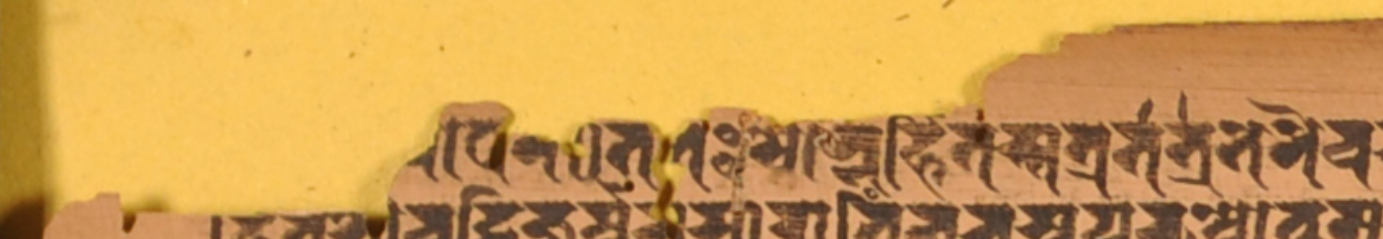
\includegraphics[scale=.21]{images/hitas_msNa.png}

[\skt{kare}] \skt{\lac\ dha\uncl{na tataḥ so 'ntar}hitas tatra tenaiva}

\msL\ (\fol380r) gives:

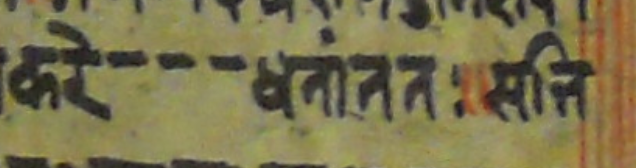
\includegraphics[scale=.3]{images/hitas01_msL.png}

\includegraphics[scale=.3]{images/hitas02_msL.png}

\skt{kare \lac\ dhatāṃ tataḥ $||$ sati hitas tatra tenaiva}
\end{quote}

\noindent
trying to make sense of the fragments. The examples above
suggest that \msL\ was copied directly from \msNa\
when the damage had already been done to \msNa. For this reason,
I have not collated its readings for \VSS\ chapters 1--12.


\medskip


%1) Śivadharmaśāstra, %(serial no. 634), fols.~1v--63r; 
%2) Śivadharmottara, %  (s. no. 635) fols.~64r--143v; 
%3) Śivadharmasaṃgraha, % (s. no. 633), fols.~144r--217v;
%4) Umāmaheśvarasaṃvāda, % (s. no. 652), fols.~218v-- 263v; 
%5) Śivopaniṣad, %(s. no. 636), fols.~264r--297v; 
%6) Uttarottaramahāsaṃvāda, % (s. no. 654), fols.~298r--324r;
%7) Vṛṣasārasaṃgraha, % (s. no. 657), fols.~325r--390r;
%8) Dharmaputrikā. % (s. no. 608), fols.~391r--406r.





\hide{
**** Kesar 537 (NGMPP C 107/7). Paper, dated to NS 803 (1682--83 CE),
174 folios. Contents: Śivadharmasaṃgraha (fols.~89r--133v);
Umāmaheśvarasaṃvāda (fols.~134r--163v); Śivopaniṣad (fols. 164r--181r);
Uttarottaramahāsaṃvāda (fols.~182r--206v); Vṛṣasārasaṃgraha
(fols.~207r--251v); Dharmaputrikā (fols. 252r--262v).

**** Kesar 597 (NGMPP C 57/5). Paper, dated to NS 863 (1742--43 CE), 257
folios. Contents: Śivadharmaśāstra (fols.~1v--41v); Śivadharmottara
(fols.~42v--92r); Śivadharmasaṃgraha (fols. 93v--138v);
Umāmaheśvarasaṃvāda (fols.~139v-- 170v); Śivopaniṣad (fols.~171v--188r);
Uttarottaramahāsaṃvāda (fols.~189v-- 213r); Vṛṣasārasaṃgraha
(fols.~214v--257r).

-- NAK 4--2537 (NGMPP B 219/3). Paper, 339 folios. Contents:
Śivadharmaśāstra (fols.~1v--58r); Śivadharmottara (fols.~59v--123v);
Śivadharmasaṃgraha (fols.~124v--161v); Umāmaheśvarasaṃvāda (fols.
162v--238v); Vṛṣasārasaṃgraha (fols.~239v--338v). GOTIT

-- NAK 4--93 (NGMPP A 1341/6). Paper, 82 folios. Contents:
Śivadharmasaṃgraha (fols.~91r¤--135v); Vṛṣasārasaṃgraha
(fols.~204r¤--243v). GOTIT

-- NAK 4--1604 (NGMPP A 1365/3). Paper, 90 folios. Contents: Śivopaniṣad
(fols.~166v--184r); Uttarottaramahāsaṃvāda (fols.~185v--210r);
Vṛṣasārasaṃgraha (fols.~211v--255r). For a description of this
manuscript, see the record in the NGMCP online catalogue:
\textless{}http://catalogue.ngmcp.uni-hamburg.de/wiki
/A\_1365-3(1)\_Śivopaniṣad\textgreater{} ASK*}

\medskip


\subsection{Kathmandu paper manuscripts}

\msdescr{(N)\msPaperA}{msPaperAdesc}
NGMCP A 1341/6, NAK 4--93. Paper, 82 folios,
probably from the 17th century (see the
description of \msPaperC\ below). 
This MS contains two texts: 
the \SDhSangr\ (\fols91r--135v) and 
the \Vss\ (\fols204r--243v). This MS was collated only for
chapters one and eight in this volume, 
but consulted often at problematic passages.
As already seen
from the folio numbers, this multiple-text
manuscript must have contained more than two
texts originally, most probably of the
Śivadharma corpus. 
The script of this MS seems extremely similar to that 
of \msPaperC, a MS dated to 1688 \CE\ (see below).
Thus it seems probable that this MS is also
from the 17th century.

\msPaperA\ is a good example to see how relatively
late witnesses, paper MSS, can be important. Its readings
are relatively independent of most palm-leaf MSS,
and seem to shed some light on what source(s) 
Naraharinath may have used because there
are a great number of instances where \Ed\ and \msPaperA\
(and \msPaperC, see below) 
read together against most other witnesses. E.g., \msCa, \msCb, \msCc, \msNa, \msNb, \msNc, \msNd, 
and \msM\ read \skt{bhāratasaṃhitām}, or a slightly
corrupt form of the same, in 1.2cd, while the two
paper MSS \msPaperA, and \msPaperC, 
and Naraharinath's \Ed\ read (a clearly wrong)
\skt{nāradasaṃhitām}. Similarly, in 1.17cd most
witnesses read \skt{vettum arhasi}, while 
\msPaperA, \msPaperC, and \Ed\ (and \msM!) read
\skt{vaktum arhasi}. In 1.44b, \msPaperA\ and
\Ed\ read \skt{mṛddhe}% 
		\footnote{\msPaperC\ reads a similar
					\skt{gṛdbhe}.}
instead of \skt{śṛṇu} and \skt{śṛṅge} 
in all other witnesses.
In some instances, the paper
MSS \msPaperA\ and \msPaperC\ give readings
that might be old or `original.' E.g., 20.40d is missing
in a great number of MSS (\msCa, \msCb, \msNa, \msNb),
\msNc\ gives (improvises?) a less than perfect 
\skt{tān nibodha dvijottamaḥ},%
		 \footnote{One would expect the vocative
		 				\skt{dvijottama}.}
while \msPaperA, \msPaperC, and \Ed\ give a similarly imperfect
\skt{vijñeyā ca manīṣibhiḥ}.%
		 \footnote{The correct sandhi would be
		 				\skt{vijñeyāś ca}.}
Sometimes these two paper MSS either alter
the text, or again, preserve older readings. 
E.g., in 16.34 \msPaperA, \msPaperC, and \Ed\
give \skt{bhagavān uvāca} against all other witnesses'
\skt{maheśvara uvāca}. After 12.30d (\skt{vipulaḥ punar abravīt}),
\msPaperA, \msPaperC, and again \Ed, insert
a somewhat unnecessary \skt{vipula uvāca}. These
and many other examples could prove that
Naraharinath used manuscripts that were close
to \msPaperA\ and \msPaperC,\label{narahari_paperms}
and some of the oddities in his edition originate in fact in 
actual readings rather than misreadings or
20th-century alterations.%
		\footnote{Compare this with 	
					\mycitep{SaivaUtopia}{58--59}, especially the
					following piece of information:
					`According to the information kindly
					provided by Diwakar Acharya (personal communication),
					it may have been based on a Devanāgarī manuscript 	
					from the time of Raṇa Bahādur Shah (1775--1806).'}

Another fascinating phenomenon in \msPaperA\ is
traces of editorial activity. There is a rather
peculiar \skt{kākapada}, or editorial sign to mark
omission, that could help us catch a perhaps
17-19th century editor red-handed while he is inspecting,
correcting, and sometimes altering the text, and 
also while he is consulting older palm-leaf MSS.
The sign can be spotted, e.g., in \msPaperA\
on top of a \skt{ku}, indicating that the syllable \skt{ru}, 
given in the top margin,
should be inserted there; 
doubled in the same MS to indicate a larger omission; 
in MS NGMPP C 57/5, another paper Śivadharma corpus
multiple-text MS, to indicate a alternative reading;
and in the much older palm-leaf MS, 
\msNa, to indicate a missing passage,
which is in fact to be found in at least two paper MSS 
(\msPaperA\ and \msPaperC) and in Naraharinath's
edition  (see Figure \ref{fig:kakapadas}).

\begin{figure}
\hspace{3em} 

\includegraphics[scale=.2]{images/mspaperA227rkakapadablurred.png}
\hfill

\includegraphics[scale=.2]{images/doublekakapada_msPaperA238r.png	}
\hfill

\includegraphics[scale=.4]{images/C57_5_kakapada7v.png}
\hfill

\includegraphics[scale=.5]{images/dottedkakapada01.png}
%
\includegraphics[scale=1]{images/dottedkakapada_small.png}
\hspace{3em}

\hspace{2em}
\msPaperA\ \fol229\recto
\hspace{1.5em}
\msPaperA\ \fol238\recto\
\hspace{.7em}
C 57/5 \fol7\verso\
\hspace{2.4em}
\msNa\ \fol45\verso
\hspace{2em}
\caption{\skt{Kākapada}s\label{fig:kakapadas}}
\end{figure}

Consulting \mycite{EinickeKorrektur}, 
a rich catalogue of editorial marks,
one gets the impression that this type 
of \cskt{kākapada}{kakapada}, which has a dot in it,
is not frequently seen. Two instances of such a 
 \cskt{kākapada}{kakapada} 
  occur in two NGMPP 
 \titleface{Viṣṇudharmaśāstra} MSS from 1661 and 1713 \CE,%
 		\footnote{MSS G 18/2 and B 218/2, 
 							\mycitep{EinickeKorrektur}{161--162 and
 										236}.}
one in the above mentioned Śivadharma MS 
NGMPP C 57/5 from 1826 \CE,%
		\footnote{\mycitep{EinickeKorrektur}{164 and 328}.} 
 and in a \titleface{Kālacakratantra} MS written 
 in old Bengali script from 1446 \CE, 
 which has (most probably much later) corrections
 in Nepālākṣara script.%
 					 \footnote{\mycitep{EinickeKorrektur}{65--66 and 328}.
 					 On p.~66, Einicke remarks: `Besonderheiten: 
 					 Korrekturen einzelner Zeichen in späterer 
 					 Newārī-Schrift am Rand'.}
 				 
It is difficult to escape the impression that
we are dealing with the same editor, whose
distinguishing mark is a \cskt{kākapada}{kakapada} 
with a dot. If indeed MS C 57/5 (1826 \CE) also bears
his hallmark, then he must have been a pundit from 
the 19th or 20th century. He seems to have performed
some rather detailed and focused editorial activities, and
must have had access to some of the old palm-leaf MSS.
One telling example for this is his marking the omission
in \msNa\ of two \skt{anuṣṭubh} verses on heavens after
\VSS\ 24.72 (see image on the right in Figure
\ref{fig:kakapadas}). 
As hinted at above, these verses, 
potentially later insertions, occur in the paper MSS
 \msPaperA\ and \msPaperC, and in Naraharinath.
To spot this, our anonymous editor had to
carefully compare the old palm-leaf MS with the 
17th-century paper MS.%
		\footnote{More on this in volume two.}
 				 
\label{msCcfirstfoliokakapada}
These observations also shed some light on
the origin of the first folio of \msCc, which is in 
a hand that looks later than that in the rest of that MS.%
		\footnote{See p.~\pageref{msCcfirstfolio}.}			 
Most old palm-leaf MSS start with \skt{karmahetuḥ śarīrasya}
etc.\ at \VSS\ 1.14ab , while the two 
paper MSS \msPaperA\ and \msPaperC, 
and Naraharinath read \skt{anarthayajña uvāca || karmahetuḥ śarīrasya}. The only palm-leaf MS that reads with 
the paper MSS is \msCc, on its only folio that is
written in a later hand. This at least tells us that
the supplied first folio in \msCc\ comes from a
source that is closer to the paper MSS than to the
old palm-leaf MSS, and it could also be another piece
of evidence for editorial activity by someone who
carefully examined these sources, and in addition,
introduced fresh contamination. \label{vipulauvaca}For this kind
of easy-to-spot contamination, a good example is
the insertion of the somewhat unnecessary
\skt{vipula uvāca} in palm-leaf MS \msCc\ after 12.30,
inspired by paper MS \msPaperA, 
and/or \msPaperC\ (see Figure \ref{fig:vipulauvaca}).
\begin{figure} 
\hfill
\includegraphics[scale=.1]{images/vipulauvaca_mscc_12.31monochrome.png}
\hfill
\includegraphics[scale=.2]{images/vipulauvaca_papermsa_12.31.png}
\hfill

\includegraphics[scale=.2]{images/vipulauvaca_msPaperC223v.png}
\hfill

\hspace{2em}
\msCc\ \fol288\verso
\hspace{5em}
\msPaperA\ \fol219\recto
\hspace{6em}
\msPaperC\ \fol223\verso
\hspace{3em}
\caption{Insertion of \skt{vipula uvāca} in \msCc\label{fig:vipulauvaca}}
\end{figure}
Note the tiny \skt{kākapada} with the dot
on the palm-leaf on the left and
the insertion in a different hand in the margin below.
It seems probable that our anonymous editor
went through some paper MSS and noted differences
in the palm-leaf MS \msCc\ (and in \msNa, see Figure
\ref{fig:kakapadas}). 

\medskip

\msdescr{(N)\msPaperC}{msPaperC}
NGMCP C107/7, NAK 9/537. Paper. Size: 
37.1~×~10.8 cm. 174 folios. This MS is
dated to NS 809 (1688--89 \CE),%
		\footnote{\raisebox{-.8em}{
\includegraphics[scale=.1]{images/msPaperCf262vDating02.png}} (\fol262v). 
		De Simini reads NS 803
		(\citeyear{DeSiminiMSSFromNepal2016}, 253 n.~51).
		I prefer reading NS 809. }
Folios 1--88 are missing. These must have contained the \SDhS\ and the \SDhU.%
			\footnote{Cf. 
				\mycitep{DeSiminiMSSFromNepal2016}{252 n.~48}. 
				See also an unfinished table of contents on \fol262r,
				which confirms that at least the \SDhS\ was part 
				of this bundle: \skt{|| asyānukramaḥ || 
				prathama śivadharmo nāma}.}
The MS thus contains only six texts:
1)~\SDhSangr\ \fols89r--133v,
2)~\Ums\ \fols134r--163v,
3)~\SivaUp\ \fols164r--181r,
4)~\Uums\ \fols182r--206v,
5)~\Vss\ \fols207r--251v, % img 8345
6)~\DharmP\ \fols252r--262v. 

The script of this 17th-century MS seems 
extremely similar to that of \msPaperA, 
therefore the latter can also be
dated to the 17th century. I collated only \VSS\ verses 1--15
as a test, the result of which failed to convince me to use this MS further.




\medskip
\subsection{Naraharinath's edition}

\msdescr{(N)\Ed}{Ed}
Much has been said of Yogi Naraharinath's pioneering
but problematic edition (the \emph{editio princeps}) 
of the Śivadharma corpus 
(\mycite{NaraharinathSivadharma}).%
			\footnote{See, e.g.,
\mycitep{DeSiminiGods2016}{66, n.\ 190};
\citeyear{DeSiminiLachmann2017}, 542,
\mycitep{BisschopUniversal}{58--59}, and
\mycitep{SaivaUtopia}{55}.}
My impression of the text of the \VSS\ in 
Naraharinath's edition (pp.~580--678) is that its quality is
considerably inferior to those of the other texts of the corpus.
It may or may not be Naraharinath's fault; 
others must have been involved in the process of transcription, and the number and nature of the innumerable mistakes all over the text may also suggest a general problem with the typesetting process. In addition to this, it is now 
gradually becoming clearer and clearer that
Naraharinath must have used late paper MSS, and
some of the oddities in his text and some of the
alterations that are difficult to explain come in fact
therefrom. See the description of \msPaperA\ and
\msPaperC\ above.
In spite of all the noise in Naraharinath's edition, it
was useful to have his text as a starting point, and it
is sometimes useful to consider his readings.
Therefore I have recorded the readings found in his
publication for all twelve chapters given in my critical edition.


\vfill
\pagebreak


\section{Editorial conventions}
\label{editorial}
\bigskip


\textit{The critically edited Sanskrit text} is to be found at the top of each page:

\begin{itemize}

%\item All Sanskrit words given in \suppl{angle brackets} have been added to the text by me as diagnostic conjectures.  These may or may not have been part of the `original' Sanskrit text.


\item Verse numbering has been supplied by the editor; none of the witnesses had any verse numbering.
\item \skt{avagraha}s are mostly supplied but sometimes found in the MSS.
                %I have not used them for crasis (e.g., {\devanagarifont })
\item Singe and double \skt{daṇḍa}s have been supplied by the editor.
        There are usually four \skt{pāda}s to a verse, but I have made arbitrary decisions
        based on sense-units, and occasionally grouped six \skt{pāda}s together as one stanza;
        none of the sources clearly indicate where a stanza ends.

\item  Headings given in [square brackets] in the critical edition and the translation 
        have been supplied to clarify the context. 
        These are not supposed to be part of the original Sanskrit text.
\end{itemize}

\bigskip
\noindent
The \textit{apparatus} is fully positive and contains a maximum of three registers. 
When all three registers are present, they contain information as follows:

\begin{itemize}
\item
The bottom register reports the variants found in the manuscripts.
Each entry starts with a verse number which is usually followed by a \skt{pāda} sign.
Both are given in boldface (e.g., \textbf{25b}). The next element is the lemma, a word, phrase, or fragment from the main text,
followed by a lemma sign ( ] ). The lemma sign is followed
by a list of the sigla of the MSS that read the same as the lemma, up to a comma. 
Next, the rejected variants are listed, each followed by the sigla of the MSS that read the given variant.
A sigma sign ($\Sigma$) stands for all available witnesses used for the given chapter,
except for one or two variants in a maximum of two witnesses.
\mssCaCbCc\ signifies all available Cambridge MSS.
A siglum followed by superscript \acorr\ marks the reading of a MS before a scribal
alteration/correction (\textit{ante correctionem}).
A siglum followed by superscript \pcorr\ marks the reading of a MS after
a scribal alteration/correction (\textit{post correctionem}). 
Corrections by the editor are marked by
`\corr' after the lemma sign (~]~\corr~), emendations by `\eme', and conjectures by `\conj'
Whenever these alterations to the text were suggested by others, I give their last names after \corr,
\eme, or \conj\ (e.g., \conj\ \textsc{Devadatta}).
%I use the expression `\textit{diagnostic conj}[\textit{ecture}]' to indicate that a conjecture is highly tentative.
The difference between corrections, emendations and conjectures is somewhat subjective in nature.
Corrections are applied in cases where the editor considers the reasons for his alteration of the text self-evident and
in little need of explanation.
In the case of an emendation, % are usually highlighted in the text by typesetting the given phrase in \textit{italics} and some explanation,
one or more parallel passages in support of the alteration, or a description of the
pal\ae ographical phenomena that resulted in the corruption,
is usually given in the footnotes to the translation of the given passage.
Effort has also been made to support conjectures
%(also typeset in \textit{italics})
with evidence, but conjectures are considered more tentative than emendations.%
        \footnote{See a more detailed discussion on emendations and
                conjectures in \Torzsok\ 1999:lxxv--lxxvi{i}i.}
%An alteration for which I have not been able to provide any supporting evidence but which I consider an improvement upon a corrupt passage is labelled a `diagnostic conj[ecture]'.%

A bullet ($\bullet$) in the apparatus separates different entries that correspond to
the same \skt{pāda}.
% \gap\ stands for a gap in the text of the MS indicated by the scribe (usually by a horizontal line).
{\devanagarifont ॰} indicates that the lemma or variant is part of a longer compound or word. 
The sign \lk\ (anceps) indicates an \skt{akṣara} illegible to me.
\lac\ indicates a complete loss of a number of \skt{akṣara}s, usually due to damage.
The number that is often placed on \lac\ (e.g., \lacwithnum{3}) indicates the approximate
number of lost \skt{akṣara}s.
Letters enclosed by (parentheses) indicate that their reading is uncertain. 
Unmetrical \skt{pāda}s are marked by `\unmetr' only when it is not fully obvious,
i.e., they are usually not marked when there is one or more syllables more 
or less than required in an \skt{anuṣṭubh} in a variant.
Sometimes `\hypometr' or `\hypermetr' are also used for hypometrical and hypermetrical verses, respectively.
%${\circ}$ stands for small circles in the MSS used as abbreviations by the scribe (e.g.\ {\dn u}${\circ}$ for {\dn uvAc}).


\item The middle register contains testimonia, i.e., passages from other sources
or from elsewhere in the \VSS\ that are parallel or similar to the
corresponding verse in the \VSS\ and that can explain, support, or
contextualise the passage or stanza in question.
An entry starts with the verse number and \skt{pāda} sign of the \VSS\ stanza in question. % and in some cases with a lemma.
I then give the title of the source from which the passage has been drawn
and the exact verse number preceded by `=' if the parallel
passage is identical with the reading of the \VSS. 
`\similar' is supplied instead of `=' if the parallel passage
is similar but not identical with the reading of the \VSS.
Testimonia are preceded by `\compare' if the passage is somewhat similar to the \textit{textus criticus} of the
\VSS, or can throw some light on it because it treats a similar subject. 
%This register of the apparatus is also the location of miscellaneous remarks on the Sanskrit text.  These remarks provide information on stanza forms, on instances of double \skt{sandhi} (e.g.\ {\dn vrd\? iEt} \jobbranyil\ {\dn vrd iEt} \jobbranyil\ {\dn vrd\?Et}% %\skt{varade} + \skt{iti} ${\rightarrow}$\ \skt{varada iti} ${\rightarrow}$\ \skt{varadeti}), on alterations to the verse numbering of the MSS, on MSS breaking off, and so on.

\item The top register reports lacun\ae{}, and missing passages, in the MSS, and also, at the beginning of
chapters, provides list of witnesses used for the given chapter.


\end{itemize}

\noindent
\textit{The transcription} of the MSS, both in the critically edited version and
in reporting variants, involves some inevitable falsification:

\begin{itemize}

\item I have not attempted to always report differences in readings between \skt{akṣara}s that are usually
        interchangeable in the Nepālākṣara MSS ({\devanagarifont ब-व} , {\devanagarifont  व-च} , {\devanagarifont त-न} ,  
                {\devanagarifont य-प} , {\devanagarifont ष-स},
                but I always report them when both readings are
                theoretically possible (e.g.\ {\devanagarifont चन्दन}-{\devanagarifont वन्दन} , {\devanagarifont जय-जप}).

%\item There is some confusion between {\dn C} and {\dn \3E3w}, {\dn X} and {\dn P}, {\dn q} and {\dn K}, {\dn G} and {\dn \38Dw}; this I always report.

\item I have ignored all instances of gemination of consonants in ligature with semivowels in the main text 
and when reporting lemmata (e.g.\ {\devanagarifont कर्म} rather than {\devanagarifont कर्म्म}), 
but I always report rejected variants as they appear in the source whenever possible. If the same rejected reading
appears with different orthography in different sources, I usually report it as it appeared in the source collated first;
thus rejected variants are also often slightly falsified.

%\item I always report my corrections of {\dn C} to {\dn QC} within words (e.g.\ {\dn e\?QC\qq{n}}) and in external \skt{sandhi} (e.g.\ {\dn n QC\38DwA{\rdt}}).

\item I have altered \skt{anusvāra}s and homorganic nasals, including \skt{m}, in the main text, as
       required by standard orthography.

\item \skt{Avagraha}s are largely missing in the MSS. I have always silently supplied them
        in the \textit{textus criticus} and in the lemmata, but I have not supplied them when reporting variants.


\end{itemize}

\vfill
\pagebreak

\blankpage

\pagebreak
% set page nember also in the edition's tex source file
%\setcounter{page}{500} % set it in the edition file (.tex, see path below)

%\section{The Sanskrit text}
\myblankchapter{A Critical Edition\\ \vspace{.4em} of\\ \vspace{.4em}Vṛṣasārasaṃgraha 1--12}{A Critical Edition of Vṛṣasārasaṃgraha 1--12}

\pagebreak

\blankpage
%\addcontentsline{toc}{chapter}{A Critical Edition of Vṛṣasārasaṃgraha 1--12}
%\addcontentsline{toc}{section}{Sanskrit Text}
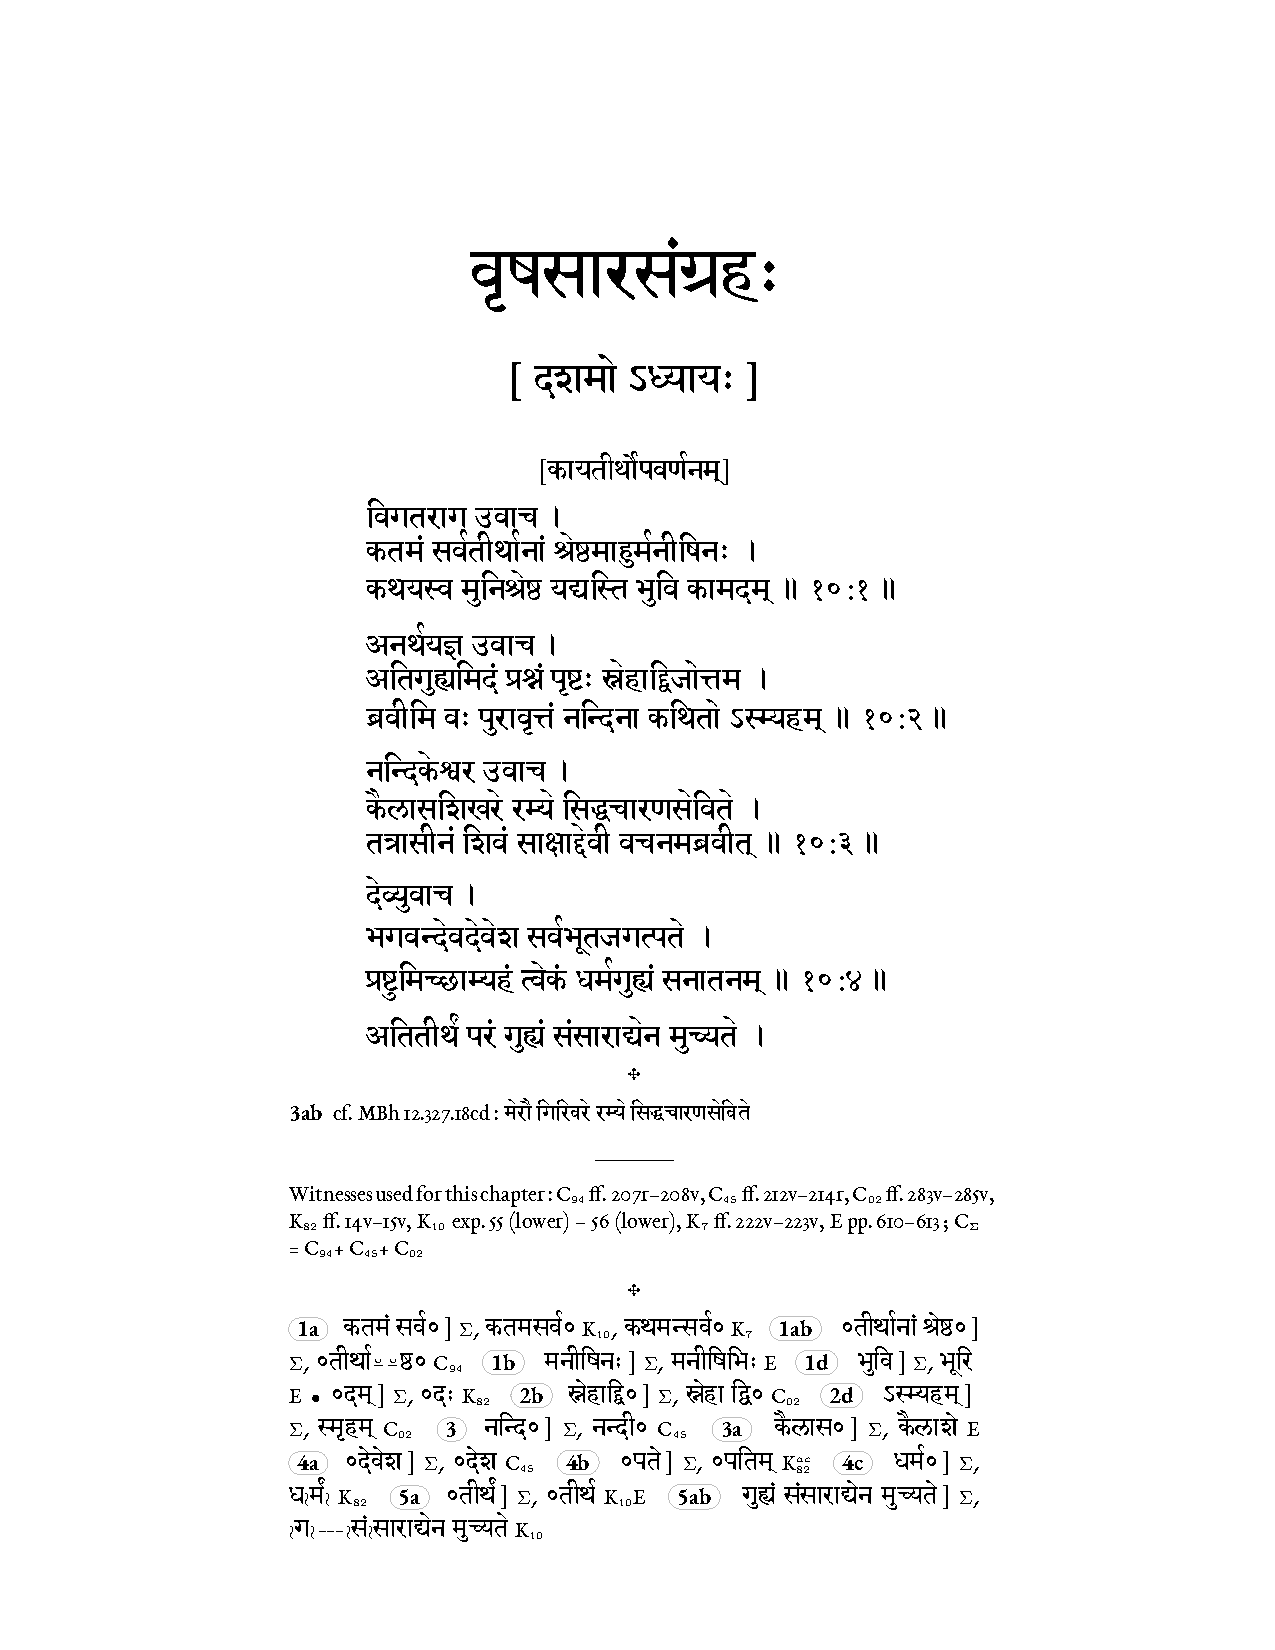
\includepdf[noautoscale, pages=-, addtotoc={1,  section, 1, Adhyāya 1, adhyaya01,
                                            20, section, 1, Adhyāya 2, adhyaya02,
                                            27, section, 1, Adhyāya 3, adhyaya03,
                                            36, section, 1, Adhyāya 4, adhyaya04,
                                            56, section, 1, Adhyāya 5, adhyaya05,
                                            62, section, 1, Adhyāya 6, adhyaya06,
                                            68, section, 1, Adhyāya 7, adhyaya07,
                                            74, section, 1, Adhyāya 8, adhyaya08,
                                            84, section, 1, Adhyāya 9, adhyaya09,
                                            93, section, 1, Adhyāya 10, adhyaya10,
                                            101, section, 1, Adhyāya 11, adhyaya11,
                                            113, section, 1, Adhyāya 12, adhyaya12}]{/home/csaba/indology/dharma_project/vrsa_edition/vrsasara_ed_devnag_xelatex.pdf}




%%%%%%%%%%%%%%%
% TRANSLATION %
%%%%%%%%%%%%%%%


\myblankchapter{An Annotated Translation of\\ Vṛṣasārasaṃgraha 1--12}{An Annotated Translation of Vṛṣasārasaṃgraha 1--12}
%\addcontentsline{toc}{section}{\Vss\ 1--12}

%FOOTNOTE
% Reformat footnotes
\makeatletter 
\renewcommand{\@makefntext}[1]{%
  \setlength{\parindent}{20pt}%
  %\begin{list}{}
  {\setlength{\labelwidth}{6mm}% 1.5em
    \setlength{\leftmargin}{0pt}%{\labelwidth}%
    \setlength{\labelsep}{10pt}%
    \setlength{\itemsep}{0pt}%
    \setlength{\parsep}{0pt}%
    \setlength{\topsep}{0pt}%
    \footnotesize}%
  %\item[\@thefnmark\hfil]
  #1% @makefnmark
  %\end{list}%
}
\makeatother 
\let\svthefootnote\thefootnote



\fancyhead[CE]{{\footnotesize \textit{Vṛṣasārasaṃgraha}}}
\fancyhead[CO]{{\footnotesize \textit{Translation of chapter 1}}}
%%%%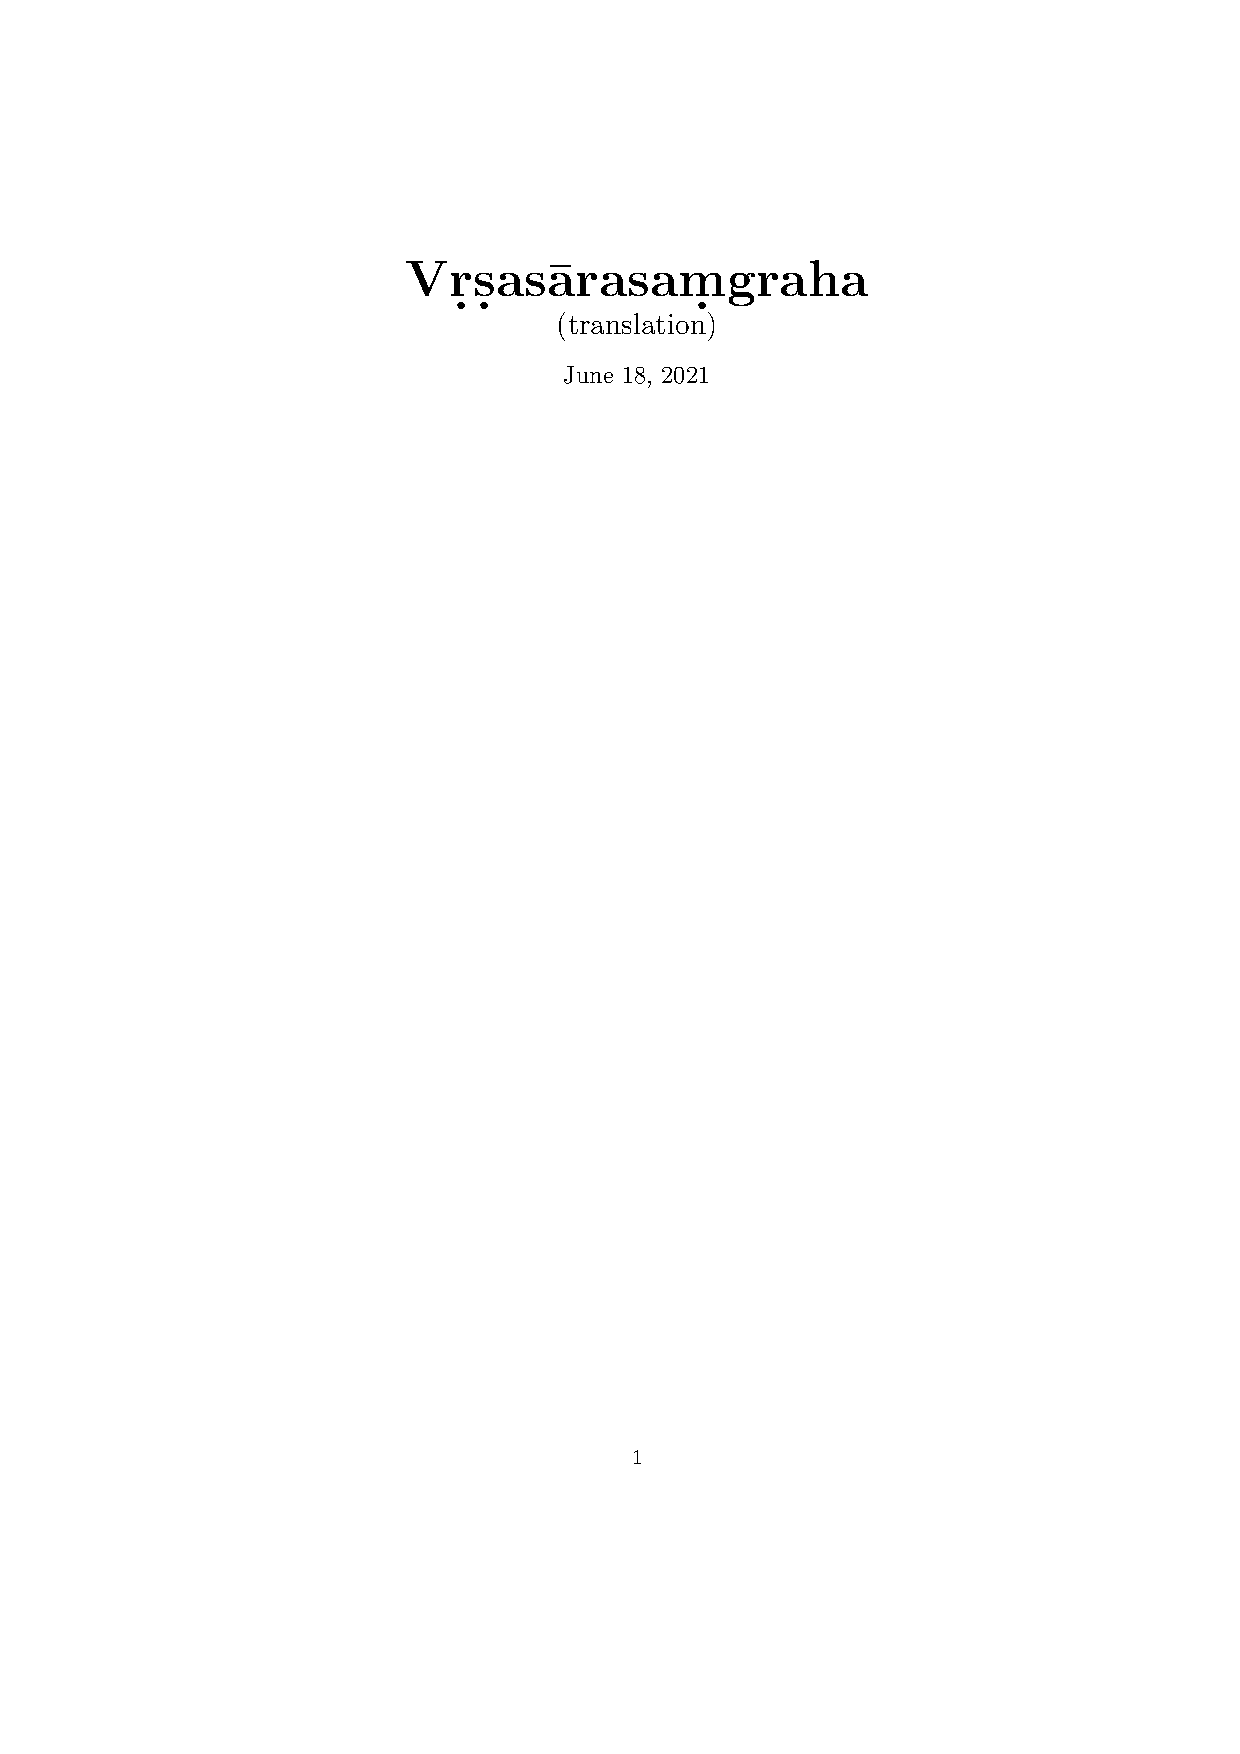
\includepdf[pages=-]{/home/csaba/indology/dharma_project/vrsa_edition/vss_translation.pdf}

% CORRECT PAGE NUMBER AFTER SKT EDITION !
\setcounter{page}{1001}
%%%%%% !TEX TS-program = xelatex
% !TEX encoding = UTF-8

% This is a simple template for a XeLaTeX document using the "article" class,
% with the fontspec package to easily select fonts.

\documentclass[11pt]{article} % use larger type; default would be 10pt

\usepackage{fontspec} % Font selection for XeLaTeX; see fontspec.pdf for documentation
\defaultfontfeatures{Mapping=tex-text} % to support TeX conventions like ``---''
\usepackage{xunicode} % Unicode support for LaTeX character names (accents, European chars, etc)
\usepackage{xltxtra} % Extra customizations for XeLaTeX

\setmainfont{Ariel} % set the main body font (\textrm), assumes Charis SIL is installed
%\setsansfont{Deja Vu Sans}
%\setmonofont{Deja Vu Mono}

% other LaTeX packages.....
\usepackage[width=12cm]{geometry} % See geometry.pdf to learn the layout options. There are lots.
\geometry{a4paper} % or letterpaper (US) or a5paper or....
%\usepackage[parfill]{parskip} % Activate to begin paragraphs with an empty line rather than an indent

\usepackage{graphicx} % support the \includegraphics command and options


\begin{document}

\textit{Qualities}

\end{document}


\
\pagebreak

\blankpage


  \chptr{prathamo 'dhyāyaḥ}
\fancyhead[CO]{{\footnotesize\textit{Translation of chapter 1}}}%

  \trchptr{Chapter One}%

  \subchptr{stutiḥ}%

  \trsubchptr{Invocation}%

  \maintext{anādimadhyāntam anantapāraṃ}%

 \nonanustubhindent \maintext{susūkṣmam avyaktajagatsusāram |}%

  \maintext{harīndrabrahmādibhir āsamagraṃ}%

 \nonanustubhindent \maintext{praṇamya vakṣye vṛṣasārasaṃgraham }||\thinspace1:1\thinspace||%
\translation{Having bowed to the One without beginning, middle, or end,\linebreak whose limits are boundless, who is most subtle, the unmanifest and the fine essence of the world---and also to Indra, Brahmā, and all the other [gods]---I shall recite [the work entitled] `A Compendium on the Essence of the Bull [of Dharma]'.\blankfootnote{1.1 Metre: \textit{upajāti}.
  \textit{Pāda} a is reminiscent of, among other famous passages, \BhG\ 11.19:
  
 
  \textit{anādimadhyāntam anantavīryam} 
  \textit{anantabāhuṃ śaśisūryanetram}\thinspace | 
 
  \textit{paśyāmi tvāṃ dīptahutāśavaktraṃ} 
  \textit{svatejasā viśvam idaṃ tapantam}\thinspace ||.
  
 
  See also \BHG\ 10.20cd:
  
 
  \textit{aham ādiś ca madhyaṃ ca bhūtānām anta eva ca}\thinspace ||.
  
 
  A faint reference to the \BHG\ seems proper at the
  beginning of a work that claims to deliver a teaching 
  based on, but also to surpass, the \MBH\ {\rm (}see following verses of the \VSS{\rm )}.
 
  Compare also, e.g., \KurmP\ 1.11.237:
  
 
  \textit{rūpaṃ tavāśeṣakalāvihīnam}
  \textit{agocaraṃ nirmalam ekarūpam}\thinspace |
  
  \textit{anādimadhyāntam anantam ādyaṃ} 
  \textit{namāmi satyaṃ tamasaḥ parastāt}\thinspace ||.
  
 
  In general, to say that a god has no beginning and no end in a temporal or spacial sense is natural
  {\rm (}\textit{anādi \dots\ antam}{\rm )}, but to have no `middle part' {\rm (}\textit{madhya}{\rm )} in these senses is slightly less so.
  Thus the rather commonly occurring phrase \textit{anādimadhyāntam} is probably a fixed expression usually 
  referring to a deity that is endless, eternal and immaterial. 
  As to which deity or what form of a deity this stanza refers to, one could argue that 
  it is Śiva, his name conspicuously missing in \textit{pāda} c, but the phrasing of the verse 
  is vague enough to keep the question somewhat open: the impersonal Brahman 
  might be another option, even more so if we look at verses 1.9--10, whose
  topic is \textit{brahmavidyā}.
 
 
  
 
  In \textit{pāda} b \textit{jagat-susāraṃ} is most probably not 
  to be interpreted as \textit{jagatsu sāraṃ} {\rm (}`the essence in the worlds'{\rm )};
  and another way to translate \textit{avyaktajagatsusāraṃ} would be: 
  `who is the fine essence of the unmanifest world.'
 
  
 
  Strictly speaking, \textit{pāda} c is unmetrical, but it is better to 
  simply acknowledge here the phenomenon of `muta cum liquida', or rather,
  \textit{krama} licence, namely
  that syllables followed by consonant clusters such as 
  \textit{ra, bra, hra, kra, śra, śya, śva, sva, dva} can be treated as light or short {\rm (}\textit{laghu}{\rm )}
  {\rm (}see pp.~\pageref{muta}\thinspace ff.{\rm )}
  Thus \textit{harīndrabrahmā}° can be treated as a regular beginning
  of an \textit{upajāti} {\rm (}\shortsyllable\ - \shortsyllable\ - -{\rm )}, the syllable 
  \textit{bra} not turning the previous syllable long {\rm (}\textit{guru}{\rm )}.
 
  
 
  The reading \textit{āsamagraṃ} in \textit{pāda} c is suspect;
  the initial \textit{ā-} before \textit{samagra} {\rm (}`whole'{\rm )} might convey some sort of
  completeness, adding the meaning `completely'
  {\rm (}see, e.g., \mycitep{KaleHigherGrammar}{226}{\rm )}.
  The fact that we could perceive the ending of \textit{pāda}s a and b 
  {\rm (}\textit{pāraṃ}--\textit{sāram}{\rm )}, as well as \textit{pāda}s c and d {\rm (}\textit{graṃ}-\textit{graham}{\rm )},
  as {\rm (}in the latter case, oddly{\rm )} rhyming pairs 
  suggests that accepting---and not emending---the reading \textit{āsamagram} could be 
  the right decision {\rm (}as suggested by Alessandro Battistini{\rm )}.
  I try to translate this verse accordingly. \msM\ gives an exciting,
  albeit unmetrical, alternative {\rm (}\textit{yat samagraṃ}{\rm )}, but
  this seems more of a guess than the correct reading.
  For some time I was considering emending \textit{āsamagraṃ}.
  The most tempting of all the possible options 
  {\rm (}\textit{arcyam/arhyam/arghyam/īḍyam/āḍhyam/āptam agraṃ, āsamastaṃ}{\rm )} 
  seemed to be \textit{āptam agraṃ},
  meaning `appointed/received/respected [by Hari, Indra,
  Brahmā etc.] as the foremost one'. The fact that 
  the \textit{akṣara}s \textit{āsam} and \textit{āptam} look similar in most
  of the scripts used in the witnesses could support this
  conjecture. \textit{āptam} could also
  possibly refer to the text itself, although then the
  syntax becomes slightly confusing: `I shall recite the
  \textit{Vṛṣasārasaṃgraha} that was first received by Hari...,' etc.
  Another candidate was \textit{āḍhyam agram}:
  `Having bowed to [Him] who contains/is rich with Hari, Indra, Brahmā,
  etc.' I have not emended the text because it is difficult
  to know if there is any need for change and if there is, which reading 
  to chose. There was no consensus when this verse was discussed 
  in our extended Śivadharma reading group.
 
  \VSS\ 1.1 is echoed in \VSS\ 20.3:
 
  \textit{nādimadhyaṃ na cāntaṃ ca yan na vedyaṃ surair api}\thinspace | 
 
  \textit{atisūkṣmo hy atisthūlo nirālambo nirañjanaḥ\thinspace ||.} 
 
  This could suggest
  that \textit{pāda} c above might be parallel with \textit{na vedyaṃ surair api}. 
  Perhaps understand \textit{asamagraṃ} [\textit{vedyaṃ}] {\rm (}`incompletely [known]{\rm )}.
 
  
 
  \textit{Pāda} d seems hypermetrical, but it can be interpreted as a \textit{vaṃśastha}
  line, a change from \textit{triṣṭubh} to \textit{jagatī} {\rm (}as suggested by Dominic Goodall{\rm )}.
 }}

  \subchptr{janamejayavaiśampāyanasaṃvādaḥ}%

  \trsubchptr{Dialogue of Janamejaya and Vaiśampāyana}%

  \maintext{śatasāhasrikaṃ granthaṃ sahasrādhyāyam uttamam |}%

  \maintext{parva cāsya śataṃ pūrṇaṃ śrutvā bhāratasaṃhitām }||\thinspace1:2\thinspace||%
\translation{Having listened to the \textit{Bhāratasaṃhitā} [i.e., the \textit{Mahābhārata}], the supreme book of a hundred thousand [verses] and a thousand chapters {\rm (}\textit{adhyāya}{\rm )}, with all its hundred sections {\rm (}\textit{parvan}{\rm )},\blankfootnote{1.2 The dialogue of Janamejaya and Vaiśampāyana makes up the outermost layer of the \VSS\ 
  {\rm (}see p.~\pageref{structure}{\rm )}, mostly containing
  general \textit{dharmaśāstric} material.
  
 
  That the \MBH\ should contain a hundred thousand verses is hinted at, e.g., in line~19 of
  Khoh Charter 2 of Śarvanātha, year 214 {\rm (}Siddham Database IN00088; 
  \textit{uktañ ca mahābhārate śatasāhasryaṃ} [understand °\textit{ryāṃ}] \textit{saṃhitāyāṃ}...{\rm )}.
  The hundred \textit{parvan}s of the \textit{Mahābhārata} are listed in \MBH\ 1.2.33--70.
  Note the use of the singular {\rm (}\textit{parva}{\rm )} in connection with numerals {\rm (}\textit{śataṃ}{\rm )},
  one of the hallmarks of this text {\rm (}see p.~\pageref{singularwithnumerals}{\rm )}.
 }}
\vfill\pagebreak


  \maintext{atṛptaḥ puna papraccha vaiśampāyanam eva hi |}%

  \maintext{janamejayena yat pūrvaṃ tac chṛṇu tvam atandritam }||\thinspace1:3\thinspace||%
\translation{Janamejaya remained unsatisfied. Listen attentively to what he asked Vaiśampāyana in the past.\blankfootnote{1.3 My emendation from the unmetrical \textit{punaḥ} to the unusual---or rather, Middle Indic
  {\rm (}\mycitep{EdgertonHybrid}{vol. 2, p. 347}{\rm )},
  and Newar {\rm (}\mycitep{JorgensenGrammar}{113}{\rm )}---\textit{puna} is based
  on the assumption that in the original the metre must have overridden 
  morphology, similarly to what may have happened in 8.44d {\rm (}Mālinī metre{\rm )}:
  \textit{na bhavati punajanma kalpakoṭyāyute 'pi}, and in 12.151c {\rm (}Sragdharā metre{\rm )}:
  \textit{garbhāvāsaṃ na ca tvan na ca punamaraṇaṃ kleśam āyāsapūrṇam}.
 
  
 
  For an unsatisfaction or dissatisfaction {\rm (}\textit{atṛpti}{\rm )} with previous 
  teachings in a somewhat similar manner to what
  Janamejaya experiences here, see, e.g., \NisvMula~1.9:
  
 
  \textit{vedāntaṃ viditaṃ deva sāṃkhyaṃ vai pañcaviṃśakam}\thinspace |
 
  \textit{na ca tṛptiṃ gamiṣyāmo hy ṛte śaivād anugrahāt}\thinspace ||.
  
 
  
 Vaiśampāyana, a Ṛṣi, disciple of Vyāsa, great-grandson of Arjuna,
  recited the \MBh\ at the snake sacrifice of 
  Janamejaya. This setting echoes of the starting point of the \MBH, see \MBH\ 1.1.8ff.
  In fact the next few verses in the \VSS\ make it clear that the \VSS\
  picks up where the \MBH\ left off: Janamejaya has heard the whole \MBh\ from
  Vaiśampāyana, but he is eager to hear more---or rather, a concise version
  of its Dharmic teachings.
  
 
  It is tempting to emend \textit{pāda} c to contain a \stemform\
  proper noun {\rm (}\textit{janamejaya}{\rm )}
  in order to maintain the metre, 
  and note how the manuscripts struggle with this \textit{pāda}. 
  \Stemform\ nouns, \textit{prātipadika}s, abound in the \VSS: 
  see p.~\pageref{stemform}.
  On the other hand, the contracted/syncopated form \textit{janmejaya} occurs, 
  e.g., in \BhagP\ 12.06.16, \BrahmaVP\ 4.14.41 and 46, and
  \NepMah\ 1.2.
  {\rm (}It is even lexicalised in \Monier{\rm )} 
  The hypermetrical form \textit{janamejayena}, and the construction finite verb + instrumental
  {\rm (}\textit{papraccha\dots janamejayena}{\rm )}, could be original {\rm (}see p.~\pageref{ergative}{\rm )}; compare 1.8 and 4.75 below.
  Alternatively, 1.3cd could be taken as a separate, and elliptical,
  sentence standing for \textit{janamejayena yac chrutaṃ pūrvaṃ tac chṛṇu}.
 }}

  \maintext{janamejaya uvāca |}%

  \maintext{bhagavan sarvadharmajña sarvaśāstraviśārada |}%

  \maintext{asti dharmaṃ paraṃ guhyaṃ saṃsārārṇavatāraṇam }||\thinspace1:4\thinspace||%
\translation{Janamejaya spoke: O venerable sir, O knower of the entire Dharma, O you who are well-versed in all the sciences {\rm (}\textit{śāstra}{\rm )}! There is a supreme and secret Dharma [that brings about] liberation from the ocean of mundane existence {\rm (}\textit{saṃsāra}{\rm )},\blankfootnote{1.4 Note \textit{dharma} as a neuter noun in \textit{pāda} c and in the next verse.
 }}

  \maintext{dvaipāyanamukhodgīrṇaṃ dharmaṃ vā yad dvijottama |}%

  \maintext{kathayasva hi me tṛptiṃ kuru yatnāt tapodhana }||\thinspace1:5\thinspace||%
\translation{that is, the Dharma that emerged from [Vyāsa] Dvaipāyana's mouth, O best of Brahmins. Teach [it] to me and help me find satisfaction at all cost, O great ascetic!\blankfootnote{1.5 The majority of the MSS consulted include a \textit{vā} in \textit{pāda} b.
  Although \msCb's reading seems somewhat smoother, that manuscript rarely preserves superior readings.
  I have therefore adopted \textit{dharmaṃ vā yad}, in which \textit{vā} probably functions in a weak sense
  {\rm (}`that is'{\rm )}.
  That the secret Dharma Janamejaya is seeking is the one taught by Vyāsa Dvaipāyana---and
  thus no real options are involved here---becomes clear in 1.6cd.
  The reading of \msM\ in \textit{pāda} b {\rm (}\textit{dharmavākyaṃ}{\rm )} is tempting but could be a later correction.
 In general, \msM's readings here are unique but probably secondary: 
  \textit{hi me tṛptiṃ} in \textit{pāda} c seems more attractive than \msM's 
  \textit{prasādena}, because it echoes \textit{atṛptaḥ} in 1.3a
 }}

  \maintext{vaiśampāyana uvāca |}%

  \maintext{śṛṇu rājann avahito dharmākhyānam anuttamam |}%

  \maintext{vyāsānugrahasamprāptaṃ guhyadharmaṃ śṛṇotu me }||\thinspace1:6\thinspace||%
\translation{Vaiśampāyana spoke: Listen with great attention, O king, to this unsurpassed narration of Dharma. Hear the secret Dharma that I received through the grace of Vyāsa. }

  \maintext{anarthayajñakartāraṃ tapovrataparāyaṇam |}%

  \maintext{śīlaśaucasamācāraṃ sarvabhūtadayāparam }||\thinspace1:7\thinspace||%
{\blankfootnote{1.7 On Anarthayajña, the interlocutor of \VSS\ 1.9--10.2 and 19.1--21.22, and
  an important figure discussed in 22.3ff, as well as a concept {\rm (}`nonmaterial sacrifice'{\rm )},
  see \mycite{KissVolume2021} and Introduction p.~\pageref{anarthayajna_person}.
 }}

  \maintext{jijñāsanārthaṃ praśnaikaṃ viṣṇunā prabhaviṣṇunā |}%

  \maintext{dvijarūpadharo bhūtvā papraccha vinayānvitaḥ }||\thinspace1:8\thinspace||%
\translation{Viṣṇu, the great Lord, assuming the form of a twice-born [Brahmin], wanted to test [Anarthayajña, the ascetic yogin] who practised nonmaterial sacrifices {\rm (}\textit{anarthayajña}{\rm )}, focused on his austerities and observances, whose conduct was virtuous and pure, and who was intent on compassion towards all living beings; therefore he [Viṣṇu] humbly asked him a question.\blankfootnote{1.8 Note the syntax here involving the agent in the instrumental
  with a finite verb {\rm (}ergative structure{\rm )}: \textit{viṣṇunā... dvijarūpadharo bhūtvā papraccha}.
  Compare 1.3 and see p.~\pageref{ergative}.
 }}
\vfill\pagebreak


  \subchptr{brahmavidyā}%

  \trsubchptr{Knowledge of Brahman}%

  \maintext{{\rm [}vigatarāga uvāca | {\rm ]}}%

  \maintext{brahmavidyā kathaṃ jñeyā rūpavarṇavivarjitā |}%

  \maintext{svaravyañjananirmuktam akṣaraṃ kimu tat param }||\thinspace1:9\thinspace||%
\translation{[Vigatarāga spoke:] How is the knowledge of the Brahman to be understood if it is devoid of form and colour? Why is that supreme syllable which is devoid of vowels and consonants the supreme one?\blankfootnote{1.9 The translation of this verse, and the reconstruction and interpretation
  of \textit{pāda} d, which is echoed in 1.10d, is slightly tentative.
  I doubt if \textit{kimu} could have the standard {\rm (}Vedic{\rm )} meaning `how much more/less'
  here. Rather \textit{u} is probably just an expletive. In general it seems that
  this verse references the syllable \textit{oṃ}, which is the impersonal Brahman.
 }}

  \maintext{anarthayajña uvāca |}%

  \maintext{anuccāryam asandigdham avicchinnam anākulam |}%

  \maintext{nirmalaṃ sarvagaṃ sūkṣmam akṣaraṃ kim ataḥ param }||\thinspace1:10\thinspace||%
\translation{Anarthayajña replied: That syllable is not to be pronounced, is unquestionable, non-dividable, consistent, spotless, all-pervading and subtle: what could be higher than that?\blankfootnote{1.10 In \textit{pāda} d, I have chosen, somewhat randomly, \textit{kim ataḥ} instead of \textit{kimu tat},
  trying to make sense of 10.9--10.
 }}

  \subchptr{kālapāśaḥ}%

  \trsubchptr{Noose of death and time}%

  \maintext{vigatarāga uvāca |}%

  \maintext{dehī dehe kṣayaṃ yāte bhūjalāgniśivādibhiḥ |}%

  \maintext{yamadūtaiḥ kathaṃ nīto nirālambo nirañjanaḥ }||\thinspace1:11\thinspace||%
\translation{Vigatarāga spoke: When the body disintegrates in the ground, in water, in fire, or [is torn apart] by jackals and other [animals], how is the supportless and spotless soul led [to the netherworld] by Yama's messengers?\blankfootnote{1.11 The word °\textit{śivā}° in \textit{pāda} b is slightly suspect, and could be the result
  of metathesis, from °\textit{viṣā}° {\rm (}`by poison'{\rm )}. Nevertheless, 
  jackals seems appropriate in this context, for they 
  are commonly associated with human corpses, death and the cremation ground
  {\rm (}see, e.g., \mycite{Ohnuma2019}{\rm )}. Furthermore, \textit{pāda} b lists phenomena
  that cause the body to disintegrate, and not causes of death; thus the reading \textit{śiva}
  is probably correct.
 }}

  \maintext{kālapāśaiḥ kathaṃ baddho nirdehaś ca kathaṃ vrajet |}%

  \maintext{svargaṃ vā sa kathaṃ yāti nirdeho bahudharmakṛt |}%

  \maintext{etan me saṃśayaṃ brūhi jñātum icchāmi tattvataḥ }||\thinspace1:12\thinspace||%
\translation{How is it bound by the nooses of death [/ time] {\rm (}\textit{kālapāśa}{\rm )}? And if it is bodiless, how can it move? And how does the [soul of a] virtuous [person] {\rm (}\textit{bahudharmakṛt}{\rm )} reach heaven if it has no body? These are my doubts. Teach me. I want to know the truth.\blankfootnote{1.12 The word \textit{kāla} has, as usual, a double meaning here: \textit{kālapāśa}
  is both Yama's noose, and also the limitations and bondage caused by time, 
  as becomes clear at the discussion on the different time units in verses 1.18--30.
 \textit{saṃśaya} seems to be treated as neuter in \textit{pāda} e.
 }}

  \maintext{anarthayajña uvāca |}%

  \maintext{atisaṃśayakaṣṭaṃ te pṛṣṭo 'haṃ dvijasattama |}%

  \maintext{durvijñeyaṃ manuṣyais tu devadānavapannagaiḥ }||\thinspace1:13\thinspace||%
\translation{Anarthayajña spoke: You are asking me about an extremely doubtful and problematic matter, O truest of the twice-born. [This is a matter that] is difficult to understand by humans, and [even] by gods {\rm (}\textit{deva}{\rm )}, demons {\rm (}\textit{dānava}{\rm )} and serpents {\rm (}\textit{pannaga}{\rm )}.\blankfootnote{1.13 Note \textit{te} used for \textit{tvayā} in \textit{pāda} a. Alternatively, taking \textit{te} as genitive, the line
  could be translated as: `I am being asked about a great 
  problem of yours that originates in doubts\dots'
 }}

  \maintext{karmahetu śarīrasya utpatti nidhanaṃ ca yat |}%

  \maintext{sukṛtaṃ duṣkṛtaṃ caiva pāśadvayam udāhṛtam }||\thinspace1:14\thinspace||%
\translation{The cause of both the birth and death of the body is karma. Good and bad deeds are called the two noos\-es.\blankfootnote{1.14 The MSS give \textit{karmahetu} in \textit{pāda} a overwhelmingly, which could work as a neuter
  \textit{bahuvrīhi} compound picking up both a stem-form \textit{utpatti} and \textit{nidhanaṃ}. 
  \textit{karmahetuḥ} {\rm (}\msCb{\rm )} is grammatically more correct, picking up the feminine \textit{utpatti},
  but a neuter stem-form \textit{utpatti} is unsurprising in this text.
 }}

  \maintext{tenaiva saha saṃyāti narakaṃ svargam eva vā |}%

  \maintext{sukhaduḥkhaṃ śarīreṇa bhoktavyaṃ karmasambhavam }||\thinspace1:15\thinspace||%
\translation{[The soul] goes to hell or heaven [bound and led] by the same [nooses of Yama's messengers, or the karmas]. Happiness and suffering, both arising from karma, are to be experienced by the body. }

  \maintext{hetunānena viprendra dehaḥ sambhavate nṛṇām |}%

  \maintext{yaṃ kālapāśam ity āhuḥ śṛṇu vakṣyāmi suvrata }||\thinspace1:16\thinspace||%
\translation{It is for this reason, O great Brahmin, that the human body is born. Now learn about that which they call the noose of time {\rm (}\textit{kālapāśa}{\rm )}, I shall teach you, O you of great observances. }

  \maintext{na tvayā viditaṃ kiñcij jijñāsyasi kathaṃ dvija |}%

  \maintext{kālapāśaṃ ca viprendra sakalaṃ vettum arhasi }||\thinspace1:17\thinspace||%
\translation{[If] you do not know anything, how could you start your investigation, O twice-born? O great Brahmin, you should know the noose of time {\rm (}\textit{kālapāśa}{\rm )} in its entirety.\blankfootnote{1.17 The variant \textit{jijñāsyasi} seems to be the lectio difficilior as opposed to
  \textit{vijñāsyasi}, but the latter could also work fine here.
 Note how \msM\ {\rm (}agreeing with two paper MSS, \msPaperA\ and \msPaperC, as well as \Ed{\rm )} 
  gives a reading {\rm (}\textit{vaktum arhasi}{\rm )} that is clearly out
  of context. This confirms that while \msM\ keeps coming up with interesting readings, 
  they are mostly to be ignored.
 }}

  \maintext{kalākalitakālaṃ ca kālatattvakalāṃ śṛṇu |}%

  \maintext{truṭidvayaṃ nimeṣas tu nimeṣadviguṇā kalā }||\thinspace1:18\thinspace||%
\translation{Learn about time {\rm (}\textit{kāla}{\rm )} which is divided into digits {\rm (}\textit{kalā}{\rm )}, [i.e., about] the division[s] {\rm (}\textit{kalā}{\rm )} of the entity [called] time {\rm (}\textit{kālatattva}{\rm )}. Two atomic units of time {\rm (}\textit{truṭi}{\rm )} are one twinkling {\rm (}\textit{nimeṣa}{\rm )}. One digit {\rm (}\textit{kalā}, cca. 1.6 second{\rm )} is twice a twinkling.\blankfootnote{1.18 \textit{Pāda}s 18d and 19a are problematic in the light of 19b, which 
  redefines \textit{kalā} in harmony with the traditional
  interpretation, see, e.g., \Arthasastra\ 2.20.33: \textit{trimśatkāṣṭhāḥ kalāḥ}.
  \nocite{Arthasastra1969}
  On divisions of time, see also, e.g., \MANU\ 1.64ff, and
  also \mycite{UnitsOfTime}.
  I have calculated 1.6 second for one \textit{kalā} backwards, starting from one day {\rm (}see 1.20ab{\rm )}.
 }}

  \maintext{kalādviguṇitā kāṣṭhā kāṣṭhā vai triṃśatiḥ kalā |}%

  \maintext{triṃśatkalā muhūrtaś ca mānuṣena dvijottama }||\thinspace1:19\thinspace||%
\translation{Two digits {\rm (}\textit{kalā}{\rm )} form one bit {\rm (}\textit{kāṣṭhā}, 3.2 seconds{\rm )}. Thirty bits {\rm (}\textit{kāṣṭhā}{\rm )} make one digit {\rm (}\textit{kalā}?, 1.6 minutes{\rm )}. Thirty digits {\rm (}\textit{kalā}{\rm )} make up one section {\rm (}\textit{muhūrta}, 48 minutes{\rm )} in human terms, O great Brahmin.\blankfootnote{1.19 Understand \textit{mānuṣena} as \textit{mānuṣasaṃkhyayā} {\rm (}1.21d{\rm )}.
 }}

  \maintext{muhūrtatriṃśakenaiva ahorātraṃ vidur budhāḥ |}%

  \maintext{ahorātraṃ punas triṃśan māsam āhur manīṣiṇaḥ }||\thinspace1:20\thinspace||%
\translation{Thirty sections {\rm (}\textit{muhūrta}{\rm )} are known to the wise as one night and day [i.e., a full day]. Thirty days and nights are taught by the wise to be one month. }

  \maintext{samā dvādaśa māsāś ca kālatattvavido janāḥ |}%

  \maintext{śataṃ varṣasahasrāṇi trīṇi mānuṣasaṃkhyayā |}%

  \maintext{ṣaṣṭiṃ caiva sahasrāṇi kālaḥ kaliyugaḥ smṛtaḥ }||\thinspace1:21\thinspace||%
\translation{One year is twelve months [according to] people who know the entity of time. The time span of three hundred and sixty thousand years by human counting is said to be the Kali age {\rm (}\textit{kali\-yuga}{\rm )}.\blankfootnote{1.21 Note how a verb {\rm (}e.g., \textit{iti vadanti, iti prāhur}{\rm )} is missing in \textit{pāda}s ab.
 }}

  \maintext{dviguṇaḥ kalisaṃkhyāto dvāparo yuga saṃjñitaḥ |}%

  \maintext{tretā tu triguṇā jñeyā catuḥ kṛtayugaḥ smṛtaḥ }||\thinspace1:22\thinspace||%
\translation{The Dvāpara age is known to be twice as long as the Kali age. The Tretā age is thrice [as long], the Kṛta age four [times as long as the Kali age].\blankfootnote{1.22 Note the \stemform\ noun \textit{yuga} in \textit{pāda} b metri causa,
  or rather the compound \textit{dvāparo-yuga-saṃjñitaḥ}
  {\rm (}the end of \textit{dvāparo} lengthened to avoid the metrical fault of two \textit{laghu}s{\rm )},
  and also \msM's unique but confused readings.
 }}

  \maintext{eṣā caturyugāsaṃkhyā kṛtvā vai hy ekasaptatiḥ |}%

  \maintext{manvantarasya caikasya jñānam uktaṃ samāsataḥ }||\thinspace1:23\thinspace||%
\translation{This is the figure related to the four ages {\rm (}\textit{yuga}{\rm )}. Multiplying it by seventy-one, the knowledge about one time-span of a Manu {\rm (}\textit{manvantara}{\rm )} has been briefly taught.\blankfootnote{1.23 Note the lengthened vowel in °\textit{yugā} {\rm (}metri causa{\rm )}.
 
  The `figure' mentioned in this verse is the sum of the duration of the four \textit{yuga}s, 
  which makes up one \textit{mahāyuga}:
  Kaliyuga = 360,000 years,
  Dvāparayuga = 720,000 years,
  Tretāyuga = 1,080,000 years,
  Kṛtayuga = 1,440,000 years; altogether 3,600,000 years. 71 \textit{mahāyuga}s make up
  a \textit{manvantara} {\rm (}= 255,600,000 years; cf. \MANU\ 1.79{\rm )}. 
  One \textit{kalpa} is 14 \textit{manvantara}s {\rm (}= 3,578,400,000 years{\rm )}. 
  Ten thousand \textit{kalpa}s are one day of Brahmā, and his night is of the same length, which
  would make one full day of Brahmā 71,568,000,000,000 human years. See next verses and,
  e.g., \mycite{GonzalezCosmic}.
 See \VSS\ 21.34ff on \textit{kalpa} etc.
 }}

  \maintext{kalpo manvantarāṇāṃ tu caturdaśa tu saṃkhyayā |}%

  \maintext{daśa kalpasahasrāṇi brahmāhaḥ parikalpitam |}%

  \maintext{rātrir etāvatī proktā munibhis tattvadarśibhiḥ }||\thinspace1:24\thinspace||%
\translation{One \ae on {\rm (}\textit{kalpa}{\rm )} is fourteen \textit{manvantara}s in total. Brahmā's day {\rm (}\textit{brahmāhar}{\rm )} is made up of ten thousand \ae ons {\rm (}\textit{kalpa}{\rm )}. [Brahmā's] night is of the same duration according to the wise who know the truth.\blankfootnote{1.24 The accepted reading \textit{kalpo} in \textit{pāda} a is probably not original, but it
  makes the sentence clearer than what is transmitted in most sources.
 \msM\ has a separator sign {\rm (}|o|{\rm )} at the end of \textit{pāda} b, as if a section ended here.
 }}

  \maintext{rātryāgame pralīyante jagat sarvaṃ carācaram |}%

  \maintext{ahāgame tathaiveha utpadyante carācaram }||\thinspace1:25\thinspace||%
\translation{When [Brahmā's] night falls, the whole moving and unmoving universe dissolves. And when [his] daylight arrives, similarly, the moving and unmoving [universe] is born here.\blankfootnote{1.25 The plural form \textit{pralīyante} in \textit{pāda} a is metri causa for \textit{pralīyate},
  perhaps also influencing \textit{utpadyante} {\rm (}for \textit{utpadyate}{\rm )} in \textit{pāda} d,
  which in turn is used here to avoid an iambic pattern
  {\rm (}- - \shortsyllable\ - \shortsyllable\ - \shortsyllable\ -{\rm )}.
  Note a general lack of a sense of grammatical number {\rm (}see p.~\pageref{number}{\rm )}.
 }}

  \maintext{parārdhaparakalpāni atītāni dvijottama |}%

  \maintext{anāgataṃ tathaivāhur bhṛgurādimaharṣayaḥ }||\thinspace1:26\thinspace||%
\translation{One \textit{para} times \textit{parārdha} [number of, i.e., two hundred quadrillion times a hundred quadrillion] \ae ons {\rm (}\textit{kalpa}{\rm )} have passed [thus far], O great Brahmin. Bhṛgu and the other sages say that the future is the same [time span].\blankfootnote{1.26 On the definition of the numbers \textit{para} and \textit{parārdha}, see verses 1.31--35.
 Note the peculiar compound \textit{bhṛgu-r-ādi-maharṣayaḥ}, for
  \textit{bhṛgvādimaharṣayaḥ}.
 }}

  \maintext{yathārkagrahatārendu bhramato dṛśyate tv iha |}%

  \maintext{kālacakraṃ bhramitvaiva viśramaṃ na ca vidmahe }||\thinspace1:27\thinspace||%
\translation{Just as the sun, the planets, the stars, and the moon are seen in this world to move in circles, so we, wandering on while riding the wheel of time {\rm (}\textit{kālacakra}{\rm )}, can never find rest.\blankfootnote{1.27 \textit{bhramato} in \textit{pāda} b seems to stand for the neuter participle \textit{bhramat}.
  Alternatively, \textit{bhramato} might mean `erroneously' {\rm (}\textit{bhrama-tas}, abl.{\rm )}, but this would
  make the verse difficult to interpret.
 I have corrected \textit{bhramatvaiva} to the standard form \textit{bhramitvaiva}, although the former
  might conceal a finite verb {\rm (}\textit{bhramāmaḥ}?{\rm )}.
 }}

  \maintext{kālaḥ sṛjati bhūtāni kālaḥ saṃharate punaḥ |}%

  \maintext{kālasya vaśagāḥ sarve na kālavaśakṛt kvacit }||\thinspace1:28\thinspace||%
\translation{Time creates living beings and time destroys them again. Everything is under the control of time. There is nothing that can bring time under control. }

  \maintext{caturdaśa parārdhāni devarājā dvijottama |}%

  \maintext{kālena samatītāni kālo hi duratikramaḥ }||\thinspace1:29\thinspace||%
\translation{Fourteen \textit{parārdha} [fourteen hundred quadrillion] divine kings, O Brahmin, have passed with time, for time is difficult to overcome.\blankfootnote{1.29 Note that \textit{samatītāni} {\rm (}neuter{\rm )} most probably picks up \textit{devarājāḥ}
  {\rm (}masculine{\rm )} in this verse, or rather \textit{devarājā} stands for
  \textit{devarājānāṃ} and \textit{samatītāni} picks up °\textit{parā\-rdhāni}. It is not clear to me
  what \textit{devarāja} {\rm (}`god king' or `divine king'{\rm )} means exactly---perhaps Indra?
 }}

  \maintext{eṣa kālo mahāyogī brahmā viṣṇuḥ paraḥ śivaḥ |}%

  \maintext{anādinidhano dhātā sa mahātmā namaskuru }||\thinspace1:30\thinspace||%
\translation{Time is [manifest] as a great yogin, as Brahmā, Viṣṇu and supreme Śiva, is beginningless and endless, is the Creator and the great soul. Pay homage [to Time]. }

  \subchptr{parārdhādi}%

  \trsubchptr{\textit{Parārdha} etc.: numbers}%

  \maintext{vigatarāga uvāca |}%

  \maintext{śrutaṃ vai kālacakraṃ tu mukhapadmaviniḥsṛtam |}%

  \maintext{parārdhaṃ ca paraṃ caiva śrotuṃ vaḥ pratidīpitam }||\thinspace1:31\thinspace||%
\translation{Vigatarāga spoke: I have now heard about the `wheel of time' {\rm (}\textit{kālacakra}{\rm )} from [your] lotus mouth. [I wish] to hear about [the terms] \textit{parārdha} and \textit{para} [mentioned above], as elaborated by you.\blankfootnote{1.31 I have corrected the unmetrical \textit{vinisṛtam} in \textit{pāda} b to \textit{viniḥsṛtam}.
  The reading of all manuscripts consulted, \textit{vinisṛtam}, 
  may be considered metrical if we interpret it, loosely, as \textit{vinisritam}.
  Also, we might read \textit{tvanmukhapadma}° {\rm (}`your lotus mouth'{\rm )} over the \textit{pāda}-boundary.
  See, e.g., \SivP\ 2.3.27.6ab: \textit{taj jñātvā nikhilaṃ devi śrutvā tvanmukhapaṃkajāt}.
 \textit{Pāda} d is suspect and my translation tentative.
  \msM's reading in \textit{pāda} d {\rm (}\textit{śrotuṃ naḥ pratidīyatāṃ}{\rm )} might make sense 
  {\rm (}`give it back/repeat it for us to hear'{\rm )}, but it sounds forced,
  as if the scribe tried to come up with a reading that he understood
  better than \textit{śrotuṃ vaḥ pratidīpitam}, the reading of the majority of the witnesses,
  which is in fact not easy to interpret. One would expect a phrase meaning
  `please tell me about these.' Finally, I have decided to take \textit{vaḥ} as 
  instrumental {\rm (}`by you'{\rm )}. Still, a verb is missing.
 }}

  \maintext{anarthayajña uvāca |}%

  \maintext{ekaṃ daśaṃ śataṃ caiva sahasram ayutaṃ tathā |}%

  \maintext{prayutaṃ niyutaṃ koṭim arbudaṃ vṛndam eva ca }||\thinspace1:32\thinspace||%
\translation{Anarthayajña spoke: One, ten, a hundred, a thousand, ten thousand {\rm (}\textit{ayuta}{\rm )}, a hundred thousand {\rm (}\textit{prayuta}{\rm )}, a million {\rm (}\textit{niyuta}{\rm )}, ten million {\rm (}\textit{koṭi}{\rm )}, a hundred million {\rm (}\textit{arbuda}{\rm )}, one billion {\rm (}\textit{vṛnda}, 10\raise .35em\hbox{\tiny 9\thinspace}{\rm )},\blankfootnote{1.32 Although the form \textit{daśa} is more standard than the accepted \textit{daśaṃ}, the latter can be original.
  See a similar teaching of numbers in \BrahmandaPur\ 3.2.91ff.
 }}

  \maintext{kharvaṃ caiva nikharvaṃ ca śaṅku padmaṃ tathaiva ca |}%

  \maintext{samudro madhyam antaṃ ca parārdhaṃ ca paraṃ tathā }||\thinspace1:33\thinspace||%
\translation{ten billion {\rm (}\textit{kharva}{\rm )}, a hundred billion {\rm (}\textit{nikharva}{\rm )}, one trillion\linebreak {\rm (}\textit{śaṅku}, 10\raise .35em\hbox{\tiny 12\thinspace}{\rm )}, ten trillion {\rm (}\textit{padma}{\rm )}, a hundred trillion {\rm (}\textit{samudra}{\rm )}, one quadrillion {\rm (}\textit{madhya}, 10\raise .35em\hbox{\tiny 15\thinspace}{\rm )}, ten quadrillion {\rm (}[\textit{an}]\textit{anta}{\rm )}, a hundred quadrillion {\rm (}\textit{parārdha}{\rm )}, and two hundred quadrillion {\rm (}\textit{para}{\rm )}.\blankfootnote{1.33 Note that \msPaperA\ inserts a line here. See apparatus.
 For \textit{anta} meaning \textit{ananta}, see 1.57. \msM's reading in \textit{pāda} d
  may be a result of an eyeskip to 1.34c.
 }}

  \maintext{sarve daśaguṇā jñeyāḥ parārdhaṃ yāvad eva hi |}%

  \maintext{parārdhadviguṇenaiva parasaṃkhyā vidhīyate }||\thinspace1:34\thinspace||%
\translation{Each should be understood as a power of ten up to \textit{parārdha}. The number corresponding to \textit{para} is twice that of \textit{parārdha}. }

  \maintext{parāt parataraṃ nāsti iti me niścitā matiḥ |}%

  \maintext{purāṇavedapaṭhitā mayākhyātā dvijottama }||\thinspace1:35\thinspace||%
\translation{There is no higher number than \textit{para}. This is my firm conviction, which is based on my readings of the Purāṇas and the Vedas and [which I have now] taught [to you], O great Brahmin.\blankfootnote{1.35 Note that \Ed\ inserts the line here that \msPaperA\ inserted above. See apparatus.
 }}

  \subchptr{brahmāṇḍam}%

  \trsubchptr{Brahmā's Egg: the Universe}%

  \maintext{vigatarāga uvāca |}%

  \maintext{brahmāṇḍaṃ kati vijñeyaṃ pramāṇaṃ jñāpitaṃ kvacit |}%

  \maintext{kati cāṅguli{-}m{-}ūrdhveṣu sūryas tapati vai mahīm }||\thinspace1:36\thinspace||%
\translation{Vigatarāga spoke: What is the extent of Brahmā's Egg {\rm (}\textit{brahmāṇḍa}{\rm )} [i.e., the universe]? Is it disclosed anywhere? From how many finger's breadths high does the sun heat the earth?\blankfootnote{1.36 The use of the singular next to numerals is one of the hallmarks of the \VSS\ 
  {\rm (}see p.~\pageref{singularwithnumerals}{\rm )}. This means that \textit{pāda} a may well refer to multiple \textit{brahmāṇḍa}s.
  Nevertheless, in the light of \VSS\ 2.2d {\rm (}\textit{pramāṇaṃ tasya vā kati}{\rm )}, I suspect that 
  the first question here could be rendered in slightly more standard Sanskrit as
  \textit{brahmāṇḍasya pramāṇaṃ kati yojanāni vijñeyaṃ}.
  \textit{cāpitaṃ kvacit} in \textit{pāda} b in the witnesses is enigmatic.
  One may conjecture \textit{prāpitaṃ} {\rm (}perhaps: `is it available somewhere?'{\rm )}.
  The intended form may have been \textit{jñātaṃ kenacit} {\rm (}`is it known by anyone?'{\rm )},
  or \textit{jñāpitaṃ} {\rm (}`is it disclosed somewhere?'{\rm )}. I have chosen the latter,
  to which 1.37 below could be a reply. Of course, \textit{cāpitaṃ} could be analysed as
  \textit{cāpi taṃ} {\rm (}possibly for \textit{cāpi tat}{\rm )}, but that would help little, unless we
  imagine that the question is `and where is it?' {\rm (}\textit{cāpi tat kva}{\rm )}.
 
  
 My emendation of \textit{cāṅguli-mūrdheṣu} to \textit{cāṅguli{-}m{-}ūrdhveṣu} {\rm (}with a hiatus-filler{\rm )} 
  is based on \textit{ūrdhvatas} in 1.60d, which is part of the reply to the question posed in this line.
  In turn, \textit{aṅguli} here triggered a conjecture in 1.60c.
 }}

  \maintext{anarthayajña uvāca |}%

  \maintext{brahmāṇḍānāṃ prasaṃkhyātuṃ mayā śakyaṃ kathaṃ dvija |}%

  \maintext{devās te 'pi na jānanti mānuṣāṇāṃ ca kā kathā }||\thinspace1:37\thinspace||%
\translation{Anarthayajña spoke: How could I enumerate [all the details of] Brahmā's Egg, O twice-born? Even the gods do not know, not to mention humans.\blankfootnote{1.37 One would expect \textit{brahmāṇḍāni} in \textit{pāda} a instead of \textit{brahmāṇḍānāṃ},
  but we should probably understand \textit{brahmāṇḍānāṃ viśeṣān prasaṃkhyātuṃ...}, or rather,
  \textit{brahmāṇḍasya viśeṣān prasaṃkhyātuṃ}.
  The structure noun in genitive + verb meaning `to tell' occurs also, e.g., in 4.69a.
  See more on this phenomenon on p.~\pageref{tellplusgen}.
 }}

  \maintext{paryāyeṇa tu vakṣyāmi yathāśakyaṃ dvijottama |}%

  \maintext{brahmaṇā yat purākhyāto mātariśvā yathā tathā }||\thinspace1:38\thinspace||%
\translation{I shall teach [you], as far as I can, in due order and truthfully, that, O great Brahmin, which Mātariśvan was taught by Brahmā in the past.\blankfootnote{1.38 The claim that Brahmā taught Mātariśvan is confirmed in 1.62cd, and
  also, e.g., in \BrahmandaPur\ 3.4.58cd {\rm (}see the apparatus{\rm )}.
 }}

  \maintext{śivāṇḍābhyantareṇaiva sarveṣām iva bhūbhṛtām |}%

  \maintext{daśa nāma diśāṣṭānāṃ brahmāṇḍe kīrtitaṃ śṛṇu }||\thinspace1:39\thinspace||%
\translation{The ten names of all the [cosmic] rulers in each of the eight directions in Brahmā's Egg {\rm (}\textit{brahmāṇḍa}{\rm )}, [which is] inside Śiva's Egg {\rm (}\textit{śivāṇḍa}{\rm )}, are being taught now, listen.\blankfootnote{1.39 My conjecture in \textit{pāda} b {\rm (}\textit{bhūbhṛtām}{\rm )} is based on the fact that the 
  readings transmitted in the MSS seem unintelligible, and, more importantly, that
  these names are said, in the subsequent verses, to belong to \textit{nāyaka}s {\rm (}`chiefs, lords'{\rm )},
  a possible synonym of \textit{bhūbhṛt} {\rm (}`a king'{\rm )}. Also, it is a minute intervention.
 
  In \textit{pāda} c, understand \textit{diśāṣṭānāṃ} as \textit{diśām aṣṭānāṃ} or \textit{digaṣṭakānāṃ}:
  again, the use of the singular in the proximity of numbers is normal in the \VSS\ {\rm (}\textit{daśa nāma}{\rm )}.
 }}

  \subchptr{bhūbhṛtāṃ nāmāni}%

  \trsubchptr{Names of the cosmic rulers}%

  \subsubchptr{pūrvataḥ}%

  \trsubsubchptr{East}%

  \maintext{sahāsahaḥ sahaḥ sahyo visahaḥ saṃhato 'sabhā |}%

  \maintext{prasaho 'prasahaḥ sānuḥ pūrvato daśa nāyakāḥ }||\thinspace1:40\thinspace||%
\translation{[1] Sahā, [2] Asaha, [3] Saha, [4] Sahya, [5] Visaha, [6] Saṃhata, [7] Asabhā, [8] Prasaha, [9] Aprasaha, [10] Sānu: [these are] the ten Leaders in the East.\blankfootnote{1.40 Note that many of the names here and in the following verses are,
  in the absence of any close parallel passage, rather insecure.
  In order to avoid the repetition of the name Saha, I take the first name here
  as feminine; Asabhā seems also to be a feminine ruler's name. Later on there
  seem to come more feminine names {\rm (}Tejā, Yamunā, Naganā, etc.{\rm )}, therefore it 
  might be correct to interpret some of the names as names of queens.
  What is clear here is that the list evokes the name Sahasrākṣa,
  one of the appellations of Indra, the guardian of the eastern direction.
 }}

  \subsubchptr{āgneye}%

  \trsubsubchptr{South-East}%

  \maintext{prabhāso bhāsano bhānuḥ pradyoto dyutimo dyutiḥ |}%

  \maintext{dīptatejāś ca tejāś ca tejā tejavaho daśa |}%

  \maintext{āgneye tv etad ākhyātaṃ yāmye śṛṇv atha bho dvija }||\thinspace1:41\thinspace||%
\translation{[1] Prabhāsa, [2] Bhāsana, [3] Bhānu, [4] Pradyota, [5] Dyutima, [6] Dyuti, [7] Dīptatejas, [8] Tejas, [9] Tejā, [10] Tejavaha: [these are] the ten [rulers] in the direction of Agni [SE]. Now listen to [the names for] Yama's region, O twice-born.\blankfootnote{1.41 Here, in the region of Agni, the names evidently evoke the image of flames.
 }}
\vfill\pagebreak


  \subsubchptr{yāmye}%

  \trsubsubchptr{South}%

  \maintext{yamo 'tha yamunā yāmaḥ saṃyamo yamuno 'yamaḥ |}%

  \maintext{saṃyano yamanoyāno yaniyugmā yanoyanaḥ }||\thinspace1:42\thinspace||%
\translation{[1] Yama, [2] Yamunā, [3] Yāma, [4] Saṃyama, [5] Yamuna, [6] Ayama, [7] Saṃyana, [8] Yamanoyāna, [9] Yaniyugmā, [10] Yanoyana.\blankfootnote{1.42 I have chosen the variant \textit{saṃyano} in \textit{pāda} c only to avoid the repetition of
  the name \textit{saṃyama}, and the variant \textit{yanoyanaḥ} in \textit{pāda} d because I suspect that
  most of the names here should begin with \textit{ya}, except for \textit{ayamaḥ}
  in \textit{pāda} b, which is little more than a guess in order to avoid the repetition of \textit{yamaḥ}.
  All the name forms in this verse are to be taken as tentative. The only 
  guiding light is the presence of \textit{ya}, reinforcing a connection with Yama.
 }}

  \subsubchptr{nairṛte}%

  \trsubsubchptr{South-West}%

  \maintext{nagajo naganā nando nagaro naga nandanaḥ |}%

  \maintext{nagarbho gahano guhyo gūḍhajo daśa tatparaḥ }||\thinspace1:43\thinspace||%
\translation{[1] Nagaja, [2] Naganā, [3] Nanda, [4] Nagara, [5] Naga, [6] Nandana, [7] Nagarbha, [8] Gahana, [9] Guhya, [10] Gūḍhaja: [these are] the ten associated with [the South-West].\blankfootnote{1.43 \textit{naga} in \textit{pāda} b is a \stemform\ noun metri causa.
 \textit{tatparaḥ} in \textit{pāda} d is be another example of a singular form next to a number {\rm (}see 1.39c above{\rm )}.
  Note that the reconstruction of these names is tentative. What is clear here is that the
  initials should be \textit{na} and \textit{ga}, probably suggesting a connection with \textit{nirṛti}, \textit{naraka}s, and \textit{nāga}s.
 }}

  \subsubchptr{vāruṇe}%

  \trsubsubchptr{West}%

  \maintext{vāruṇena pravakṣyāmi śṛṇu vipra nibodha me |}%

  \maintext{babhraḥ setur bhavodbhadraḥ prabhavodbhavabhājanaḥ |}%

  \maintext{bharaṇo bhuvano bhartā daśaite varuṇālayāḥ }||\thinspace1:44\thinspace||%
\translation{I shall teach you [the names] in Varuṇa's region [in the west]. Listen, O Brahmin, learn from me. [1] Babhra, [2] Setu, [3] Bhava, [4] Udbhadra, [5] Prabhava, [6] Udbhava, [7] Bhājana, [8] Bharaṇa, [9] Bhuvana, and [10] Bhartṛ: these ten dwell in Varuṇa's region [in the west].\blankfootnote{1.44 Varuṇa upholds {\rm (}\textit{bibharti/bharati}{\rm )} the sky and the earth. This could be the reason why 
  these names include \textit{bharaṇa} and \textit{bhartṛ}.
 }}

  \subsubchptr{vāyavye}%

  \trsubsubchptr{North-West}%

  \maintext{nṛgarbho 'suragarbhaś ca devagarbho mahīdharaḥ |}%

  \maintext{vṛṣabho vṛṣagarbhaś ca vṛṣāṅko vṛṣabhadhvajaḥ }||\thinspace1:45\thinspace||%
\translation{[1] Nṛgarbha, [2] Asuragarbha, [3] Devagarbha, [4] Mahīdhara, [5] Vṛṣabha, [6] Vṛṣagarbha, [7] Vṛṣāṅka, [8] Vṛṣabhadhvaja,\blankfootnote{1.45 The connection between \textit{vṛṣa} and the north-west or Vāyu is not evident to me. 
  In a tantric context, a western position is more standard for \textit{vṛṣa}, see, e.g.,
  \mycitep{Pancavaranastava}{40}.
 }}

  \maintext{jñātavyaś ca tathā samyag vṛṣajo vṛṣanandanaḥ |}%

  \maintext{nāyakā daśa vāyavye kīrtitā ye mayā dvija }||\thinspace1:46\thinspace||%
\translation{[9] Vṛṣaja, and [10] Vṛṣanandana: these are to be known properly as the ten leaders in Vāyu's region [in the north-west], as I taught them, O twice-born.\blankfootnote{1.46 Note how \msM\ deviates here again in a significant way.
 }}

  \subsubchptr{uttare}%

  \trsubsubchptr{North}%

  \maintext{sulabhaḥ sumanaḥ saumyaḥ suprajaḥ sutanuḥ śivaḥ |}%

  \maintext{sataḥ satya layaḥ śambhur daśa nāyakam uttare }||\thinspace1:47\thinspace||%
\translation{[1] Sulabha, [2] Sumana, [3] Saumya, [4] Supraja, [5] Sutanu, [6] Śiva, [7] Sata, [8] Satya, [9] Laya, [10] Śambhu: [these are] the ten leaders in the north.\blankfootnote{1.47 I prefer the form \textit{sumanaḥ} to the more standard \textit{sumanāḥ} {\rm (}\msNc{\rm )} in \textit{pāda} a
  because it suits the slightly irregular language of the \VSS\ {\rm (}see pp.~\pageref{language}{\rm )}
  and because the solitary reading of \msNc\ may well only be an attempt to
  standardise. It is also not inconceivable that \textit{sumanaḥ} stands compounded 
  with \textit{saumyaḥ}.
 Note how \textit{daśa nāyakam} {\rm (}neuter singular for masculine plural{\rm )}
  could again be an example for the use of the singular 
  next to a number in \textit{pāda d}. It seems that here it is the northern region
  that is associated with Śiva, rather than the north-east, the \textit{īśāna} direction, 
  which is occupied by Brahmā in the next verse. 
  {\rm (}In a tantric context, Brahmā is sometimes associated with the north-east, see, e.g.,
  \mycitep{Pancavaranastava}{39}.{\rm )}
  I have left \textit{satya} in \stemform.
 }}

  \subsubchptr{īśāne}%

  \trsubsubchptr{North-East}%

  \maintext{indu bindu bhuvo vajra varado vara varṣaṇaḥ |}%

  \maintext{ilano valino brahmā daśeśāneṣu nāyakāḥ }||\thinspace1:48\thinspace||%
\translation{[1] Indu, [2] Bindu, [3] Bhuva, [4] Vajra, [5] Varada, [6] Vara, [7] Varṣaṇa, [8] Ilana, [9] Valina, [10] Brahmā: [these are] the ten rulers in the Īśāna direction [i.e., in the north-east].\blankfootnote{1.48 I consider \textit{indu, bindu} and \textit{vajra} \stemform\ nouns.
 The north-east seems to be occupied by Brahmā, and by rulers whose names should
  somehow evoke Brahmā's name.
 }}

  \subsubchptr{madhyame}%

  \trsubsubchptr{Center}%

  \maintext{aparo vimalo moho nirmalo mana mohanaḥ |}%

  \maintext{akṣayaś cāvyayo viṣṇur varado madhyame daśa }||\thinspace1:49\thinspace||%
\translation{[1] Apara, [2] Vimala, [3] Moha, [4] Nirmala, [5] Mana, [6] Mohana, [7] Akṣaya, [8] Avyaya, [9] Viṣṇu, [10] Varada: [these are] the ten [leaders] in the centre.\blankfootnote{1.49 Note that the last three lists above have been associated 
  with Śiva, Brahmā and Viṣṇu, respectively, and here, in a layer
  of the text that can be labelled Vaiṣṇava {\rm (}see pp.~\pageref{structure}{\rm )}, it is Viṣṇu that
  seems to occupy a central position. \textit{mana mohanaḥ} {\rm (}or \textit{nirmalonmana}{\rm )} in \textit{pāda} b may
  sound like one single name, but we are forced to separate these two words
  {\rm (}\textit{mana} being in \stemform\ metri causa{\rm )} to arrive at a list of ten names.
 }}

  \subsubchptr{parivārāḥ}%

  \trsubsubchptr{Subordinates}%

  \maintext{sarveṣāṃ daśa{-}m{-}īśānāṃ parivāraśataṃ śatam |}%

  \maintext{śatānāṃ pṛthag ekaikaṃ sahasraiḥ parivāritam }||\thinspace1:50\thinspace||%
\translation{Each of the ten rulers has a retinue of a hundred subordinates. Each one of [these] hundred is surrounded by a thousand subordinates.\blankfootnote{1.50 I take \textit{daśa-m-īśānāṃ} as a split compound {\rm (}\textit{daśeśānāṃ}{\rm )}.
  It is conceivable that each of the above ninety rulers has ten subordinates, 
  therefore each group of ten rulers has a hundred subordinates altogether,
  but the original idea may have been that each one of the above ninety 
  rulers has a hundred subordinates. Alternatively, this verse may only refer to 
  the central group of ten rulers mentioned in 1.49, and each one of them has
  a hundred subordinates.
 }}

  \maintext{sahasreṣu ca ekaikam ayutaiḥ parivāritam |}%

  \maintext{ayutaṃ prayutair vṛndaiḥ prayutaṃ niyutair vṛtam }||\thinspace1:51\thinspace||%
\translation{Each one of the thousand is surrounded by ten thousand [subordinates]; the ten thousand is surrounded by a multitude of a hundred thousand; the hundred thousand by a million;\blankfootnote{1.51 We are forced to follow \Ed's reading in \textit{pāda} c in order to make sense of this passage.
  My correction in \textit{pāda} d is motivated by the same. Note that \textit{vṛnda} is not a number in this line. 
  Elsewhere in this chapter \textit{vṛnda} is the word that signifies `a billion.'
 }}

  \maintext{ekaikasya parīvāro niyutaḥ pṛthag eva ca |}%

  \maintext{koṭibhir daśakoṭyena ekaikaḥ parivāritaḥ }||\thinspace1:52\thinspace||%
\translation{[that is] each one has a retinue of a million {\rm (}\textit{niyuta}{\rm )} [subordinates]. [Then those] are surrounded by ten million {\rm (}\textit{koṭi}{\rm )} [subordinates]; [they in turn] by a hundred million {\rm (}\textit{daśakoṭi}{\rm )}.\blankfootnote{1.52 It seems that \textit{pāda}s ab repeat what has been stated in 1.51cd.
 °\textit{koṭyena} stands for °\textit{koṭyā} {\rm (}thematisation{\rm )}.
  Note how the scribe of \msM\ gets confused at 1.52c due to an eyeskip and 
  fully regains control only at 1.54b.
 }}

  \maintext{daśakoṭiṣu ekaikaṃ vṛndavṛndabhṛtair vṛtam |}%

  \maintext{vṛndavargeṣu ekaikaṃ kharvabhiḥ parivāritam }||\thinspace1:53\thinspace||%
\translation{Each one of the hundred million is surrounded by a billion {\rm (}\textit{vṛnda}{\rm )} subordinates {\rm (}\textit{bhṛta}{\rm )}. Each one in these groups of a billion {\rm (}\textit{vṛnda}{\rm )} is surrounded by ten billion {\rm (}\textit{kharva}{\rm )} [subordinates]. }

  \maintext{kharvavargeṣu ekaikaṃ daśakharvagaṇair vṛtam |}%

  \maintext{daśakharveṣu ekaikaṃ śaṅkubhiḥ parivāritam }||\thinspace1:54\thinspace||%
\translation{Each in these groups of ten billion {\rm (}\textit{kharva}{\rm )} is surrounded by a hundred billion {\rm (}\textit{daśakharva}{\rm )}. Each of those hundred billion is surrounded by a trillion {\rm (}\textit{śaṅku}{\rm )} [deities]. }

  \maintext{śaṅkubhiḥ pṛthag ekaikaṃ padmena parivāritam |}%

  \maintext{padmavargeṣu ekaikaṃ samudraiḥ parivāritam }||\thinspace1:55\thinspace||%
\translation{Each of those one trillion is surrounded by ten trillion {\rm (}\textit{padma}{\rm )}. Each of those ten trillion is surrounded by a hundred trillion {\rm (}\textit{samudra}{\rm )}.\blankfootnote{1.55 Note that in \textit{pāda} a \textit{śaṅkubhiḥ} stands for \textit{śaṅkūṣu} {\rm (}instrumental for locative{\rm )}.
 }}

  \maintext{samudreṣu tathaikaikaṃ madhyasaṃkhyais tu tair vṛtam |}%

  \maintext{madhyasaṃkhyeṣu ekaikam anantaiḥ parivāritam }||\thinspace1:56\thinspace||%
\translation{And each of those hundred trillion is surrounded by those whose number is one quadrillion {\rm (}\textit{madhya}{\rm )}. Each of those quadrillion is surrounded by ten quadrillion {\rm (}\textit{ananta}{\rm )}. }

  \maintext{ananteṣu ca ekaikaṃ parārdhaparivāritam |}%

  \maintext{parārdheṣu ca ekaikaṃ pareṇa parivāritam |}%

  \maintext{eṣa vai kathito vipra śakyaṃ sāṃkhyam udīritam }||\thinspace1:57\thinspace||%
\translation{Each of those ten quadrillion is surrounded by a hundred quadrillion {\rm (}\textit{parā\-rdha}{\rm )}. Each of those hundred quadrillion is surrounded by two hundred quadrillion {\rm (}\textit{para}{\rm )}. Thus it is taught, O Brahmin. The enumeration [of the rulers of the Brahmāṇḍa] has been taught as much as it is possible. }

  \subchptr{pramāṇam}%

  \trsubchptr{Measurements}%

  \maintext{pramāṇaṃ śṛṇu me vipra saṃkṣepād bruvato mama |}%

  \maintext{candrodaye pūrṇamāsyāṃ vapur aṇḍasya tādṛśam }||\thinspace1:58\thinspace||%
\translation{Listen to me and learn about the measurements [of Brahmā's Egg], O Brahmin, I shall teach [you] in a concise manner. The body of the Egg is like that of [the moon] at moonrise on the day of the full moon. }

  \maintext{koṭikoṭisahasraṃ tu yojanānāṃ samantataḥ |}%

  \maintext{aṇḍānāṃ ca parīmāṇaṃ brahmaṇā parikīrtitam }||\thinspace1:59\thinspace||%
\translation{The whole circumference of the Egg has been declared by Brahmā to be ten million {\rm (}\textit{koṭi}{\rm )} times a thousand times ten million \textit{yojana}s.\blankfootnote{1.59 I suspect that the plural form \textit{aṇḍānāṃ} is accidental and what is meant
  is a singular.
 }}

  \maintext{saptakoṭisahasrāṇi saptakoṭiśatāni ca |}%

  \maintext{viṃśakoṭiṣv aṅgulīṣu ūrdhvatas tapate raviḥ }||\thinspace1:60\thinspace||%
\translation{The Sun shines from the height of seven thousand seven hundred and twenty \textit{koṭi} finger's breadth.\blankfootnote{1.60 This verse is the reply to the question in 1.36cd, which contains the word \textit{aṅguli}:
  this hints at the possibility that the unintelligible \textit{gulmeṣu} transmitted in most of the
  witnesses might be corrupted from \textit{aṅgulīṣu}; hence my conjecture, resulting
  in a \textit{ra-vipulā}. For reference, the distance given here {\rm (}7,720 \textit{koṭi aṅgula}s \similar\
  1--1.5 million km{\rm )} is about a hundred times smaller than the modern 
  astronomical distance to the Sun {\rm (}\similar\ 150 million km{\rm )}.
 }}

  \maintext{pramāṇaṃ nāma saṃkhyā ca kīrtitāni samāsataḥ |}%

  \maintext{brahmāṇḍaṃ cāprameyāṇāṃ lakṣaṇaṃ parikīrtitam }||\thinspace1:61\thinspace||%
\translation{The numbers pertaining to the measurements have been taught in brief. The characteristics of the unmeasurable Brahmāṇḍa[s] have been taught.\blankfootnote{1.61 Note the mixture of different grammatical genders and numbers in this verse. 
  Understand \textit{pramāṇeṣu saṃkhyāḥ kīrtitāḥ samāsataḥ} and 
  \textit{brahmāṇḍānām aprameyānāṃ}, or \textit{brahmāṇḍasyāprameyasya}, which is even metrical.
 }}

  \subchptr{purāṇam}%

  \trsubchptr{Redactors of the Purāṇa{\rm [}s{\rm ]}}%

  \maintext{purāṇāśīsahasrāṇi śatāni dvijasattama |}%

  \maintext{brahmaṇā kathitaṃ pūrṇaṃ mātariśvā yathātatham }||\thinspace1:62\thinspace||%
\translation{O truest of the twice-born, the Purāṇa[s of] 8,000,000 [verses] were taught by [1] Brahmā to [2] Mātariśvan [= Vāyu] in their entirety, in their true form.\blankfootnote{1.62 \textit{Pāda} a should probably be analysed and interpreted as 
  \textit{purāṇam brahmaṇā kathitam}, or rather, \textit{purāṇānām aśītisahasrāṇi śatāni ślokāni
  brahmaṇā kathitāni}.
  Alternatively, \textit{pāda} a may have originally read \textit{purāṇāni sahasrāṇi},
  and then the initial number of verses transmitted by Brahmā is
  a hundred thousand. That the number refers to the number of \textit{śloka}s
  transmitted is confirmed in 1.65d: \textit{viṃśatślokasahasrikam}.
 
  
 
  In \textit{pāda} d, either understand \textit{mātariśvā} {\rm (}nom.{\rm )} as \textit{mātariśvānaṃ} {\rm (}acc.{\rm )} or emend
  \textit{kathitaṃ} to \textit{kathitaḥ} in the sense `Mātariśvan was taught,' echoing 1.38cd:
  \textit{brahmaṇā yat purākhyāto mātariśvā yathā tathā}.
  
 
  On the idea that initially there was only one Purāṇa, see, e.g.,
  \mycitep{RocherPuranas1986}{41ff}.
  Compare the list in the \VSS\ to a list of twenty-eight \textit{vedavyāsa}s, from
  Brahmā to Vyāsa Dvaipāyana, in \VisnuP\ 3.3.10--19 {\rm (}which is similar to \BrahmandaPur\ 1.35.117ff{\rm )},
  taught by Parāśara, the twenty-sixth \textit{vyāsa}
  of this list and our text {\rm (}in the numbering that I add here I follow
  the translation in \mycitep{Visnupurana_tr}{178--179}{\rm )}:
  
 
  \textit{vedavyāsā vyatītā ye aṣṭāviṃśati sattama~|} 
 
  \textit{caturdhā yaiḥ kṛto vedo dvāpareṣu punaḥ punaḥ~||} 
 
  \textit{dvāpare prathame vyastāḥ svayaṃ vedāḥ }[1]\textit{ svayaṃbhuvā~|} 
 
  \textit{dvitīye dvāpare caiva vedavyāsaḥ }[2]\textit{ prajāpatiḥ~||} 
 
  \textit{tṛtīye }[3]\textit{ cośanā vyāsaś caturthe ca }[4]\textit{ bṛhaspatiḥ~| } 
 
  [5]\textit{ savitā pañcame vyāsaḥ }[6]\textit{ mṛtyuḥ ṣaṣṭhe smṛtaḥ prabhuḥ~|| } 
 
  \textit{saptame ca }[7]\textit{ tathaivendro }[8]\textit{ vasiṣṭhaś cāṣṭame smṛtaḥ~| } 
 
  [9]\textit{ sārasvataś ca navame }[10]\textit{ tridhāmā daśame smṛtaḥ~|| } 
 
  \textit{ekādaśe tu }[11]\textit{ trivṛṣā }[12]\textit{ bhāradvājas tataḥ param~| } 
 
  \textit{trayodaśe }[13]\textit{ cāntarikṣo }[14]\textit{ varṇī cāpi caturdaśe~|| } 
 
  [15]\textit{ trayyāruṇaḥ pañcadaśe ṣoḍaśe tu }[16]\textit{ dhanaṃjayaḥ~| } 
 
  [17]\textit{ kratuṃjayaḥ saptadaśe }[18]\textit{ ṛṇajyo 'ṣṭādaśe smṛtaḥ~|| } 
 
  \textit{tato vyāso }[19]\textit{ bharadvājo bharadvājāt tu }[20]\textit{ gautamaḥ~| } 
 
  \textit{gautamād uttamo vyāso }[21]\textit{ haryātmā yo 'bhidhīyate~|| } 
 
  \textit{atha haryātmano }[22]\textit{ venaḥ smṛto vājaśravās tu yaḥ~| } 
 
  \textit{somaḥ śuṣmāyaṇas tasmāt }[23]\textit{ tṛṇabindur iti smṛtaḥ~|| } 
 
  [24]\textit{ ṛkṣo 'bhūd bhārgavas tasmād vālmīkir yo 'bhidhīyate~| } 
 
  \textit{tasmād asmatpitā }[25]\textit{ śaktir vyāsas tasmād }[26]\textit{ ahaṃ mune~|| } 
 
  [27]\textit{ jātukarṇo 'bhavan mattaḥ kṛṣṇadvaipāyanas }[28]\textit{ tataḥ~| } 
 
  \textit{aṣṭaviṃśatir ity ete vedavyāsāḥ purātanāḥ~|| }
 
  
 
  Another relevant passage is \BrahmandaPur\ 3.4.58cd--67 {\rm (}\similar\ \VAYUP\ 2.41.58--67{\rm )}.
  Note how Tṛṇabindu is, perhaps by mistake, different from Somaśuṣma/Śuṣmāyaṇa here,
  but, more importantly, note Amitabuddhi of \VSS\ 1.75b appearing at the end of this list:
  
 
  [1] \textit{brahmā dadau śāstram idaṃ purāṇaṃ }[2]\textit{ mātariśvane~|| } 
 
  \textit{tasmāc }[3]\textit{ cośanasā prāptaṃ tasmāc cāpi }[4]\textit{ bṛhaspatiḥ~| } 
 
  \textit{bṛhaspatis tu provāca }[5]\textit{ savitre tadanantaram~|| } 
 
  \textit{savitā }[6]\textit{ mṛtyave prāha mṛtyuś }[7]\textit{ cendrāya vai punaḥ~| } 
 
  \textit{indraś cāpi }[8]\textit{ vasiṣṭāya so 'pi }[9]\textit{ sārasvatāya ca~|| } 
 
  \textit{sārasvatas }[10]\textit{ tridhāmne 'tha tridhāmā ca }[11]\textit{ śaradvate~| } 
 
  \textit{śaradvāṃs tu }[12]\textit{ triviṣṭāya so }[13]\textit{ 'ntarikṣāya dattavān~|| } 
 
  [14]\textit{ carṣiṇe cāntarikṣo vai so 'pi }[15]\textit{ trayyāruṇāya ca~| } 
 
  \textit{trayyāruṇād }[16]\textit{ dhanañjayaḥ sa vai prādāt }[17]\textit{ kṛtañjaye~|| } 
 
  \textit{kṛtañjayāt }[18]\textit{ tṛṇañjayo }[19]\textit{ bharadvājāya so 'py atha~| } 
 
  [20]\textit{ gautamāya bharadvājaḥ so 'pi }[21]\textit{ niryyantare punaḥ~|| } 
 
  \textit{niryyantaras tu provāca tathā }[22]\textit{ vājaśravāya vai~| } 
 
  \textit{sa dadau }[23]\textit{ somaśuṣmāya sa cādāt }[24]\textit{ tṛṇabindave~|| } 
 
  \textit{tṛṇabindus tu }[25]\textit{ dakṣāya dakṣaḥ provāca }[26]\textit{ śaktaye~| } 
 
  \textit{śakteḥ }[27]\textit{ parāśaraś cāpi garbhasthaḥ śrutavān idam~|| } 
 
  \textit{parāśarāj }[28]\textit{ jātukarṇyas tasmād }[29]\textit{ dvaipāyanaḥ prabhuḥ~| } 
 
  \textit{dvaipāyanāt punaś cāpi }[30]\textit{ mayā prāptaṃ dvijottama~|| } 
 
  \textit{mayā caitat punaḥ proktaṃ }[31]\textit{ putrāyāmitabuddhaye~| } 
 
  \textit{ity eva vākyaṃ brahmādiguruṇāṃ samudāhṛtam~||} 
 
  
 
  The list of \textit{vedavyāsa}s in \LinPu\ 1.7.15--18 includes these twenty-five names:
  Kratu, Satya, Bhārgava, Aṅgiras, Savitṛ,
  Mṛtyu, Śatakratu, Vasiṣṭha, Sārasvata, Tridhāman,
  Trivṛta, Śatatejas, Tarakṣu, Āruṇi, Kṛtaṃjaya,
  Ṛtaṃjayo, Bharadvāja, Gautama, Vācaśravas, Tṛṇabindu,
  Rūkṣa, Śakti, Jātūkarṇya, Kṛṣṇa Dvaipāyana.
 }}

  \maintext{vāyunā pāda saṃkṣipya prāptaṃ cośanasaṃ purā |}%

  \maintext{tenāpi pāda saṃkṣipya prāptavāṃś ca bṛhaspatiḥ }||\thinspace1:63\thinspace||%
\translation{Vāyu abridged the verses and then gave [the Purāṇas] to [3] Uśanas. He [Uśanas] also abridged the verses, and [4] Bṛhaspati received them.\blankfootnote{1.63 Note the \stemform\ noun \textit{pāda} twice in this verse and 
  the slightly odd grammatical structure in \textit{pāda} b, {\rm (}\textit{purāṇaṃ}{\rm )} \textit{prāptam uśanasam} 
  {\rm (}`the Purāṇa reached Uśanas'{\rm )},
  as opposed to the solution in \textit{pāda} d with \textit{prāptavān}.
 }}

  \maintext{bṛhaspatis tu provāca sūryaṃ triṃśatsahasrikam |}%

  \maintext{pañcaviṃśatsahasrāṇi mṛtyuṃ prāha divākaraḥ }||\thinspace1:64\thinspace||%
\translation{Bṛhaspati taught 30,000 [verses] to [5] Sūrya [the Sun]. Divākara [= the Sun] taught 25,000 [verses] to [6] Mṛtyu [Death].\blankfootnote{1.64 \textit{Pāda} a is a ma-\textit{vipulā}, or simply a \textit{pathyā} if \textit{pra} in \textit{provāca}
  does not turn the previous syllable long {\rm (}\mutacumliquida{\rm )}.
 }}

  \maintext{ekaviṃśatsahasrāṇi mṛtyunendrāya kīrtitam | }%

  \maintext{indreṇāha vasiṣṭhāya viṃśatślokasahasrikam }||\thinspace1:65\thinspace||%
\translation{Mṛtyu taught 21,000 [verses] to [7] Indra. Indra taught 20,000 verses to [8] Vasiṣṭha. }

  \maintext{aṣṭādaśasahasrāṇi tena sārasvatāya tu |}%

  \maintext{sārasvatas tridhāmāya sahasradaśa sapta ca }||\thinspace1:66\thinspace||%
\translation{He[, Vasiṣṭha, taught] 18,000 [verses] to [9] Sārasvata. Sārasvata [taught] 17,000 [verses] to [10] Tridhāma[n]. }

  \maintext{ṣoḍaśānāṃ sahasrāṇi bharadvājāya vai tataḥ |}%

  \maintext{daśa pañcasahasrāṇi trivṛṣāya abhāṣata }||\thinspace1:67\thinspace||%
\translation{[Tridhāman taught] 16,000 verses to [11] Bharadvāja. [Bharadvāja] taught 15,000 verses to [12] Trivṛṣa. }

  \maintext{caturdaśasahasrāṇi antarīkṣāya vai tataḥ |}%

  \maintext{trayyāruṇiṃ sahasrāṇi trayodaśa abhāṣata }||\thinspace1:68\thinspace||%
\translation{[Trivṛṣa] then [taught] 14,000 verses to [13] Antarīkṣa. [Antarīkṣa] taught 13,000 [verses] to [14] Trayyāruṇi. }

  \maintext{trayyāruṇis tu viprendro dhanaṃjayam abhāṣata |}%

  \maintext{dvādaśāni sahasrāṇi saṃkṣipya punar abravīt }||\thinspace1:69\thinspace||%
\translation{Trayyāruṇi, the great Brahmin, having abridged them again, taught 12,000 [verses] to [15] Dhanaṃjaya. }

  \maintext{kṛtaṃjayāya samprāpto dhanaṃjayamahāmuniḥ |}%

  \maintext{kṛtaṃjayād dvijaśreṣṭha ṛṇaṃjayamahātmane }||\thinspace1:70\thinspace||%
\translation{Dhanaṃjaya, the great sage, handed [them] over to [16] Kṛtaṃjaya. [That recension was transmitted] from Kṛtaṃjaya, O best of the twice-born, to [17] noble Ṛṇaṃjaya.\blankfootnote{1.70 Note the odd structure in \textit{pāda}s ab: \textit{dhanaṃjayaḥ kṛtaṃjayāya samprāptaḥ}, 
  for a more standard \textit{dhanaṃjayena {\rm (}\textit{purāṇam}{\rm )} samprāpitaṃ kṛtaṃjayam} 
  {\rm (}`the Purāṇa was transmitted to Kṛtaṃjaya'{\rm )}.
 }}

  \maintext{ṛṇañjayāt punaḥ prāpto gautamāya maharṣiṇe |}%

  \maintext{gautamāc ca bharadvājas tasmād dharyadvatāya tu }||\thinspace1:71\thinspace||%
\translation{Then from Ṛṇaṃjaya it was given to [18] Gautama, the great sage; from Gautama to [19] Bharadvāja, from him to [20] Haryadvata.\blankfootnote{1.71 The structure of \textit{pāda}s ab is as odd as that of 1.70ab. What was
  intended is probably \textit{ṛṇañjayena prāpitaṃ gautamāya}. Many of the
  syntactic oddities in this and other chapters might betray an influence
  of classical Newar. See pp.~\pageref{newar}.
 The name Haryadvata in \textit{pāda} d seem to be a variant on the attested forms
  Haryatvata and Haryātman {\rm (}the latter is in the list of \textit{vedavyāsa}s in 
  \VISNUP\ 3.3.16--17, see note to 1.62 above{\rm )}.
 }}

  \maintext{rājaśravās tataḥ prāptaḥ somaśuṣmāya vai tataḥ |}%

  \maintext{somaśuṣmāt tataḥ prāptas tṛṇabindus tu bho dvija }||\thinspace1:72\thinspace||%
\translation{Then [21] Rājaśravas received it; and then [22] Somaśuṣma; then from Somaśuṣma [23] Tṛṇabindu received it, O twice-born.\blankfootnote{1.72 The syntax is again slightly odd here. The intention may have been
  \textit{prāpitaṃ rājaśravasā somaśuṣmāya... tatas tṛṇabindunā prāptam}.
 }}

  \maintext{tṛṇabindus tu vṛkṣāya vṛkṣaḥ śaktim abhāṣata |}%

  \maintext{śaktiḥ parāśaraṃ prāha jatukarṇāya vai tataḥ }||\thinspace1:73\thinspace||%
\translation{Tṛṇabindu taught it to [24] Vṛkṣa; Vṛkṣa to [25] Śakti [the father of Parāśara]. Śakti taught it to [26] Parāśara; then [Parāśara] to [27] Jatukarṇa.\blankfootnote{1.73 In other list of \textit{vedavyāsa}s, Tṛṇabindu hands the Purāṇas down to 
  Ṛkṣa, Rūkṣa or Dakṣa {\rm (}see note to 1.62 above{\rm )}; \textit{vṛkṣa} in \textit{pāda} a
  is probably a corrupted form.
 The name Jatukarṇa may be a corrupted form of Jātū- or Jātukarṇa.
 }}

  \maintext{dvaipāyanaṃ tu provāca jatukarṇo maharṣiṇam |}%

  \maintext{romaharṣāya samprāpto dvaipāyanamahāmuniḥ }||\thinspace1:74\thinspace||%
\translation{Jatukarṇa taught it to [28] [Vyāsa] Dvaipāyana, the great sage. Dvaipāyana, the great sage, gave it to [29] Romaharṣa.\blankfootnote{1.74 \textit{Pāda}s ab are a \textit{pathyā} if \textit{pra} in \textit{provāca}
  does not turn the previous syllable long {\rm (}\mutacumliquida{\rm )}.
 The syntax of \textit{pāda}s cd echoes that of 1.70ab above.
 }}

  \maintext{romaharṣeṇa provāca putrāyāmitabuddhaye |}%

  \maintext{daśa dve ca sahasrāṇi purāṇaṃ samprakāśitam |}%

  \maintext{mānuṣāṇāṃ hitārthāya kiṃ bhūyaḥ śrotum icchasi }||\thinspace1:75\thinspace||%
\translation{Romaharṣa taught the Purāṇa[s] of 12,000 [verses], now fully revealed, to his son, [30] Amitabuddhi, for the benefit of humankind. What else do you wish to know?\blankfootnote{1.75 Romaharṣa is usually considered to be the same person as Sūta, disciple of Vyāsa Dvaipāyana.
  
  
 
  In \BrahmandaPur\ 3.4.67ab {\rm (}\textit{mayā caitat punaḥ proktaṃ putrāyāmitabuddhaye}, see note to 
  1.62 above{\rm )}, Amitabuddhi is clearly the name {\rm (}or epithet{\rm )} of Romaharṣa's son. 
  This suggests that the reading \textit{romaharṣāya} in some of the MSS
  in \textit{pāda} a is a mistake for \textit{romaharṣaś ca}, or something similar. MS \msM\ is either transmitting a
  syntactically problematic reading {\rm (}\textit{romaharṣeṇa}{\rm )} that may nevertheless be more 
  original than that preserved in most other witnesses, or its scribe is attempting
  to correct the text. Supposing the former, I have accepted \msM's reading.
 Note that the extent of the transmitted text {\rm (}12,000 \textit{śloka}s{\rm )} has not changed since Trayyāruṇi
  {\rm (}1.69{\rm )}.
 
 
  Manuscripts \msCc\ and \msM\ place the \textit{iti} of the colophon at the end of the last \textit{śloka}, before
  the \textit{daṇḍa}s, thus: \textit{icchasīti}\thinspace ||O|| {\rm (}\msCc{\rm )} and \textit{icchasi iti}\thinspace ||O|| {\rm (}\msM{\rm )}.
  Note also that \msM\ gives the number of \textit{śloka}s in this chapter as `77', which is close to
  the number of verses yielded by this critical edition. The scribe of \msM\ struggled 
  with eyeskips in this chapter, therefore it seems unlikely that he himself
  counted the number of verses he had copied and arrived at this very figure.
  More likely, he reproduced the number from his exemplar.
 }}

\centerline{\maintext{\dbldanda\thinspace iti vṛṣasārasaṃgrahe brahmāṇḍasaṃkhyā nāmādhyāyaḥ prathamaḥ\thinspace\dbldanda}}
\translation{Here ends the first chapter in the \textit{Vṛṣasārasaṃgraha} called Description of Brahmā's Egg.}

  \chptr{dvitīyo 'dhyāyaḥ}
\fancyhead[CO]{{\footnotesize\textit{Translation of chapter 2}}}%

  \trchptr{Chapter Two}%

  \maintext{vigatarāga uvāca |}%

  \maintext{śrutaṃ mayā janāgreṇa brahmāṇḍasya tu nirṇayam |}%

  \maintext{pramāṇaṃ varṇarūpaṃ ca saṃkhyā tasya samāsataḥ }||\thinspace2:1\thinspace||%
\translation{Vigatarāga spoke: I have heard the description of Brahmā's Egg {\rm (}\textit{brahmāṇḍa}{\rm )} from [you,] the best of men, its extent, colour, form, and the numbers associated with it, in a concise manner.\blankfootnote{2.1 It is unlikely that \textit{janāgreṇa} picks up \textit{mayā} {\rm (}`by me, the best of men'{\rm )}.
  Instead, I suppose that this instrumental could be understood as `through the best of man,' 
  or rather, simply taken as an ablative {\rm (}`from the best of men'{\rm )}.
 }}

  \maintext{śivāṇḍeti tvayā prokto brahmāṇḍālayakīrtitaḥ |}%

  \maintext{kīdṛśaṃ lakṣaṇaṃ jñeyaṃ pramāṇaṃ tasya vā kati }||\thinspace2:2\thinspace||%
\translation{You mentioned Śiva's Egg {\rm (}\textit{śivāṇḍa}{\rm )} as taught to be the receptacle of Brahmā's Egg {\rm (}\textit{brahmāṇḍa}{\rm )}. What are its characteristics and how much is its extent?\blankfootnote{2.2 The location where the Śivāṇḍa was mentioned is verse 1.39a above.
 }}

  \maintext{kasya vā layanaṃ jñeyaṃ pramāṇaṃ vātra vāsinaḥ |}%

  \maintext{kā vā tatra prajā jñeyā ko vā tatra prajāpatiḥ }||\thinspace2:3\thinspace||%
\translation{And whose dwelling place is it? And [what] is the extent of the inhabitants thereof? What kind of subjects live there? And who is the ruler {\rm (}\textit{prajāpati}{\rm )} there?\blankfootnote{2.3 \textit{vā layanaṃ} in \textit{pāda} a may stand for \textit{vā-ālayanaṃ}, in the sense of \textit{vā-ālayaṃ}.
  The questions in this verse are most probably answered in verses 2.26--33, and if my
  interpretation is correct there, \textit{pramāṇaṃ vātra vāsinaḥ} {\rm (}understand \textit{vāsināṃ}{\rm )} 
  and \textit{pāda}~c should refer to the number of inhabitants in the five regions of Īśāna, Tatpuruṣa, etc.,
  deities who are referred to here in \textit{pāda}s a and possibly d.
 }}

  \subchptr{śivāṇḍasaṃkhyā}%

  \trsubchptr{Summary of the Śivāṇḍa}%

  \maintext{anarthayajña uvāca |}%

  \maintext{śivāṇḍalakṣaṇaṃ vipra na tvaṃ praṣṭum ihārhasi |}%

  \maintext{daivatair api kā śaktir jñātuṃ draṣṭuṃ ca tattvataḥ }||\thinspace2:4\thinspace||%
\translation{Anarthayajña spoke: Please don't ask me about the characteristics of Śiva's Egg {\rm (}\textit{śivāṇḍa}{\rm )}, O Brahmin. How could even the gods have the power to truly know and see Śiva's Egg? }

  \maintext{agamyagamanaṃ guhyaṃ guhyād api samuddhitam |}%

  \maintext{na prabhur netaras tatra na daṇḍyo na ca daṇḍakaḥ }||\thinspace2:5\thinspace||%
\translation{The path leading to it is not to be trodden, it is more secret than any secret, and it is lofty. There is no master or servant there, nobody to be punished and no punisher.\blankfootnote{2.5 \textit{samuddhitam} in \textit{pāda} b is suspect. Emending it to \textit{samuddhṛtam} would not be 
  fully satisfactory, and the readings transmitted in the witnesses are problematic. 
  \msM, a MS not collated for this chapter, gives a confusing reading: \textit{sa\uncl{murdhni}dam}. 
  I doubt if \Ed's \textit{samṛddhidam} {\rm (}`yielding success'{\rm )} is the correct reading.
  Perhaps \textit{samudāhṛtam} {\rm (}`declared, talked about as'{\rm )}, or \textit{samāvṛtam} {\rm (}`guarded'{\rm )} was meant.
  It is not inconceivable that \textit{agamyagahanaṃ} in \msCc\ {\rm (}and in \msM\msPaperA;
  `it is inaccessible because of its depth'{\rm )} is original and
  is to be contrasted with \textit{samuddhṛtam} {\rm (}`lofty'{\rm )}. One also wonders if
  \textit{guhād} could be the right reading, and in what sense, in \textit{pāda} b.
 }}

  \maintext{na satyo nānṛtas tatra suśīlo no duḥśīlavān |}%

  \maintext{nānṛjur na ca dambhitvaṃ na tṛṣṇā na ca īrṣyatā }||\thinspace2:6\thinspace||%
\translation{There are no truthful or untruthful people there, no moral or immoral people, no crooked people, no hypocrisy, no thirst or envy.\blankfootnote{2.6 Strictly speaking \textit{duḥśīlavān} in \textit{pāda} b is unmetrical; understand or pronounce \textit{duśīlavān}.
 \textit{īrṣyatā} {\rm (}for \textit{īrṣyā}, see 2.7a{\rm )} is a form rarely attested.
 }}

  \maintext{na krodho na ca lobho 'sti na māno 'sti na sūyakaḥ |}%

  \maintext{īrṣyā dveṣo na tatrāsti na śaṭho na ca matsaraḥ }||\thinspace2:7\thinspace||%
\translation{There is no anger or greed there, no arrogance or discontent {\rm (}[\textit{a}]\textit{sūyaka}{\rm )}, no envy or hatred, no cheaters and no jealousy.\blankfootnote{2.7 \textit{na sūyakaḥ} in \textit{pāda} b stands for \textit{nāsūyakaḥ} {\rm (}\textit{na asūyakaḥ}{\rm )} metri causa.
 }}

  \maintext{na vyādhir na jarā tatra na śoko 'sti na viklavaḥ |}%

  \maintext{nādhamaḥ puruṣas tatra nottamo na ca madhyamaḥ }||\thinspace2:8\thinspace||%
\translation{There is no disease, no aging, no grief and no agitation there, there are no inferior or superior people and there is nobody in-between. }

  \maintext{notkṛṣṭo mānavas tasmin striyaś caiva śivālaye |}%

  \maintext{na nindā na praśaṃsāsti matsarī piśuno na ca }||\thinspace2:9\thinspace||%
\translation{There are no privileged men or women there in Śiva's abode, no reproach or praise, no selfish or treacherous people. }

  \maintext{garvadarpaṃ na tatrāsti krūramāyādikaṃ tathā |}%

  \maintext{yācamāno na tatrāsti dātā caiva na vidyate }||\thinspace2:10\thinspace||%
\translation{There is no pride or arrogance there, no cruelty or trickery and so on. There are no beggars and no donors there. }

  \maintext{anarthī vraja tatrasthaḥ kalpavṛkṣasamāśritaḥ |}%

  \maintext{na karma nāpriyas tatra na kaliḥ kalaho na ca }||\thinspace2:11\thinspace||%
\translation{Go without material desires {\rm (}\textit{anarthin}{\rm )}. Once there, you will rest beneath a wishing tree. There is no karma there, no enemy, no Kali age, and no fighting.\blankfootnote{2.11 Note the term \textit{anarthī} in \textit{pāda} a: it may be connected with the notion
  and with our interlocutor Anarthayajña.
 My emendation in \textit{pāda} c from \textit{na priyas} {\rm (}`no lover/husband'{\rm )} to \textit{nāpriyas} {\rm (}`no enemy'{\rm )} 
  may not be strictly necessary but it seems more meaningful than the transmitted readings.
 }}

  \maintext{dvāparo na ca na tretā kṛtaṃ cāpi na vidyate |}%

  \maintext{manvantaraṃ na tatrāsti kalpaś caiva na vidyate }||\thinspace2:12\thinspace||%
\translation{There is no Dvāpara, no Tretā, no Kṛta age; no Manu-eras {\rm (}\textit{manvantara}{\rm )}, and no \ae ons {\rm (}\textit{kalpa}{\rm )} exist there.\blankfootnote{2.12 On \textit{manvantara}s and \textit{kalpa}s, see 1.22--23 above.
 }}

  \maintext{āhūtasamplavaṃ nāsti brahmarātridinaṃ tathā |}%

  \maintext{na janmamaraṇaṃ tatra āpadaṃ nāpnuyāt kvacit }||\thinspace2:13\thinspace||%
\translation{No universal floods of destruction occur there, nor are there days and nights of Brahmā. There is no birth or death, and no catastrophes ever arise.\blankfootnote{2.13 \textit{āhūtasamplava} for the more widely attested form \textit{ābhūtasamplava} occurs, e.g.,
  in some MSS transmitting \SDhS\ 10.77 and 81 {\rm (}see \mycite{RitesOfFasting}{\rm )}.
 }}

  \maintext{na cāśāpāśabaddho 'sti rāgamohaṃ na vidyate |}%

  \maintext{na devā nāsurās tatra na yakṣoragarākṣasāḥ }||\thinspace2:14\thinspace||%
\translation{No one is bound by the noose of hope; there is no passion or delusion. There are no gods or demons there, nor any Yakṣas, Serpents, or Rākṣasas. }

  \maintext{na bhūtā na piśācāś ca gandharvā ṛṣayas tathā |}%

  \maintext{tārāgrahaṃ na tatrāsti nāgakiṃnaragāruḍam }||\thinspace2:15\thinspace||%
\translation{There are neither Ghosts nor Piśācas, no Gandharvas and no Ṛṣis. There are no planets, no Nāgas, Kiṃnaras or Garuḍa-like creatures. }

  \maintext{na japo nāhnikas tatra nāgnihotrī na yajñakṛt |}%

  \maintext{na vrataṃ na tapaś caiva na tiryaṅnarakaṃ tathā }||\thinspace2:16\thinspace||%
\translation{There are no recitations or daily rituals; no one performs the Agnihotra, and there are no sacrificers. There are no religious observances, no austerities, and no `animal hell'.\blankfootnote{2.16 The phrase of \textit{tiryaṅnaraka} appears in \MBH\ 3.181.18ab: 
  \textit{aśubhaiḥ karmabhiḥ pāpās tiryaṅnarakagāminaḥ}. \mycite{GanguliMBh} translates \textit{tiryaṅ} 
  in this line from the \MBH\
  separately as `in a crooked way,' but I suspect that in the \VSS\ \textit{tiryaṅnaraka} has
  more to do with \textit{tiryaggati}, i.e., the state of 
  being reduced to animal existence, being reborn as an animal, or entering hell in animal form. 
  Cf. \MBH\ Suppl. 13.15.2615--16:
 
  \textit{nṛṣu janma labhante ye karmaṇā madhyamāḥ smṛtāḥ}\thinspace |
 
  \textit{tiryaṅnarakagantāro hy adhamās te narādhamāḥ}\thinspace ||; 
 
  and \Ums\ 6.1:
 
  \textit{avamanyanti ye viprān sarvaloke namaskṛtān}\thinspace |
 
  \textit{narakaṃ yānti te sarve tiryagyoniṃ vrajanti ca~||}. 
  
 I suspect that \textit{nātirya}° in the witnesses is only a scribal mistake for \textit{na tirya}°.
 }}

  \maintext{tasyeśānasya devasya aiśvaryaguṇavistaram |}%

  \maintext{api varṣaśatenāpi śakyaṃ vaktuṃ na kenacit }||\thinspace2:17\thinspace||%
\translation{No one could ever measure the extent of the divine powers of the god, not even in a hundred years.\blankfootnote{2.17 My translation of \textit{aiśvaryaguṇa}° is tentative. It could be taken as a \textit{dvandva} compound
  {\rm (}e.g., `supremacy and qualities'{\rm )}. The expression \textit{sarva}° or \textit{aṣṭaiśvaryaguṇopeta}
  occurs frequently---e.g., in \SivP\ 7.2.8.28ab, \SkandaP\ 55.30cd, and \SDhU\ 2.6, 79, 125, 127,
  with \textit{aiśvarya} most probably referring to the eight \textit{siddhi}s \textit{aṇiman, laghiman}, etc.
  De Simini {\rm (}2016a, 386{\rm )},\nocite{DeSiminiGods2016} e.g., 
  translates \textit{sarvaiśvaryaguṇopetaḥ} in \SDhU\ 2.127 as
  `endowed with all the qualities of lordship.'
 }}

  \maintext{harecchāprabhavāḥ sarve paryāyeṇa bravīmi te |}%

  \maintext{devamānuṣavarjyāni vṛkṣagulmalatādayaḥ }||\thinspace2:18\thinspace||%
\translation{All are born by Hara's wish. I shall teach [them] to you one by one---gods, humans, trees, bushes, creepers, and the rest.\blankfootnote{2.18 Treat \textit{pāda} a as if it were the object of \textit{bravīmi}.
 Note the gender confusion in this verse. In \textit{pāda} c, °\textit{varjyāni} is suspect. 
  I take it as if it stood for \textit{vargāḥ/vargāṇi}, and not in the sense of `excluding,'
  because gods and people are in fact, albeit vaguely, mentioned below.
 }}

  \maintext{parārdhadviguṇotsedho vistāraś ca tathāvidhaḥ |}%

  \maintext{anekākārapuṣpāṇi phalāni ca manoharam }||\thinspace2:19\thinspace||%
\translation{The height [of the Śivāṇḍa] is two \textit{parārdha}s, and [its] width is the same. There are lovely flowers of many forms there, as well as delightful fruits.\blankfootnote{2.19 I understand \textit{pāda} a as \textit{parārdhadviguṇa utsedho}, i.e., as an example of double \textit{sandhi}.
  On the other hand, °\textit{sedho} is only my conjecture, and \textit{pāda} a
  may have originally referred to something else than the Śivāṇḍa.
  Note the number confusion in \textit{pāda} d, and also that two \textit{parārdha}s is one \textit{para}, 
  the highest possible number according to verses 1.34--35 above. The number may refer to
  any unit of length, but 2.23 below suggests that it is \textit{yojana}s.
 }}

  \maintext{anye kāñcanavṛkṣāṇi maṇivṛkṣāṇy athāpare |}%

  \maintext{pravālamaṇiṣaṇḍāś ca padmarāgaruhāṇi ca }||\thinspace2:20\thinspace||%
\translation{There are also golden trees and jewel trees, thickets of coral gems, and ruby plants,\blankfootnote{2.20 Note that both \textit{anye} and \textit{apare} here pick up neuter nouns {\rm (}gender confusion{\rm )}.
 }}

  \maintext{svādumūlaphalāḥ skandhalatāviṭapapādapāḥ |}%

  \maintext{kāmarūpāś ca te sarve kāmadāḥ kāmabhāṣiṇaḥ }||\thinspace2:21\thinspace||%
\translation{tasty roots and fruits, and trees with creepers twining around their trunks and branches. All are shape-shifters, fulfilling every desire and whispering seductively.\blankfootnote{2.21 My conjectures in \textit{pāda}s ab result in a compound spanning the c\ae sura, which
  may have been the reason why this line got corrupted.
 }}

  \maintext{tatra vipra prajāḥ sarve anantaguṇasāgarāḥ |}%

  \maintext{tulyarūpabalāḥ sarve sūryāyutasamaprabhāḥ }||\thinspace2:22\thinspace||%
\translation{There[, in the Śivāṇḍa], O Brahmin, all the subjects are oceans of endless virtues. They are all equally beautiful and strong, and they shine like millions of suns. }

  \maintext{parārdhadvayavistāraṃ parārdhadvayam āyatam |}%

  \maintext{parārdhadvayavikṣepaṃ yojanānāṃ dvijottama }||\thinspace2:23\thinspace||%
\translation{[Śiva's Egg] is two \textit{parārdha}s long and two \textit{parā\-rdha}s wide, and two \textit{parā\-rdha}s is its [vertical] extension, [measured] in \textit{yojana}s, O great Brahmin.\blankfootnote{2.23 Both \textit{pāda} a and c may be treated as containing two words, the first in
  stem form: \textit{parārdhadvaya vistāraṃ} and \textit{parārdhadvaya vikṣepaṃ}.
 }}

  \maintext{aiśvaryatvaṃ na saṃkhyāsti balaśaktiś ca bho dvija |}%

  \maintext{adhordhvo na ca saṃkhyāsti na tiryañ caiti kaścana }||\thinspace2:24\thinspace||%
\translation{[Īśāna's] divinity cannot be expressed in numbers, nor can [His] strength and power, O twice-born. [The distances within Śiva's Egg], both above and below, likewise cannot be expressed in numbers. None can traverse it.\blankfootnote{2.24 \textit{Pāda}s ab are an echo of 2.17b.
 \textit{kaścana} in \textit{pāda} d forces us to accept the reading in \msNapcorr\msNc\ {\rm (}\textit{caiti}{\rm )},
  as opposed to \textit{ceti} in the remaining witnesses. Alternatively, translate as
  `[The distances within Śiva's Egg] downwards and 
  upwards and horizontally cannot be expressed in numbers, some people say.'
 }}

  \maintext{śivāṇḍasya ca vistāram āyāmaṃ ca na vedmy aham |}%

  \maintext{bhogam akṣaya tatraiva janmamṛtyur na vidyate }||\thinspace2:25\thinspace||%
\translation{[Indeed,] I do not know the length and breadth of Śiva's Egg. Enjoyment there is undecaying; there is neither birth nor death.\blankfootnote{2.25 \textit{Pāda} c is transmitted in an unmetrical form and with a gender problem in the witnesses
  {\rm (}\textit{bhogam akṣayas}, including paper MS \msPaperA, not collated here{\rm )},
  hence my emendation using a \stemform\ noun,
  a phenomenon frequently seen in this text. But note that \textit{bhoga} is normally masculine,
  therefore we may also see a hiatus-filler in-between the two words: \textit{bhoga-m-akṣaya}.
 }}

  \maintext{śivāṇḍamadhyam āśritya gokṣīrasadṛśaprabhāḥ |}%

  \maintext{parārdhaparakoṭīnām īśānānāṃ smṛtālayaḥ }||\thinspace2:26\thinspace||%
\translation{In the centre of Śiva's Egg, [creatures] shine like cow's milk. [It is] said to be the region {\rm (}\textit{ālaya}{\rm )} of those belonging to Īśāna, one and a half \textit{para} crore in number.\blankfootnote{2.26 Note the \stemform\ \textit{smṛta} in \textit{pāda} d {\rm (}cf. 2.29d{\rm )}.
  I understand \textit{īśānānāṃ} as \textit{aiśānānāṃ}.
  
 
  Īśāna is traditionally the upward-looking face of Śiva;
  his region is positioned at the centre here.
  Note that the somewhat cryptic third \textit{pāda}s here and in the coming verses
  may or may not refer to the number of creatures dwelling in the given region. 
  They may instead indicate the extent of the given region, although the numbers are much
  higher than one would expect after verse 2.23; in fact, the second \textit{para}
  might simply function in the way \textit{adhika} normally does---the number could
  be `half a \textit{para} plus a crore.'
 }}

  \maintext{bālasūryaprabhāḥ sarve jñeyās tatpuruṣālaye |}%

  \maintext{parārdhaparakoṭīnāṃ pūrvasyāṃ diśam āśritāḥ }||\thinspace2:27\thinspace||%
\translation{They are all like the rising sun in the region of Tatpuruṣa, one and a half \textit{para} crore in number, dwelling in the east.\blankfootnote{2.27 The genitive of \textit{parārdhaparakoṭīnāṃ} is baffling here and in the coming verses,
  but I suspect that again the expression gives the number of subjects living in the given region.
  \textit{pūrvasyāṃ} is meant to mean \textit{pūrvāṃ} {\rm (}cf. \textit{dakṣiṇāṃ, paścimāṃ}, and \textit{uttarāṃ} in the next verses{\rm )};
  note how \msNb\ tries to save the construction by reading \textit{diśi-m-}.
 
  This verse conforms to the traditional view that Śiva's Tatpuruṣa-face
  is looking towards the eastern direction.
 }}

  \maintext{bhinnāñjanaprabhāḥ sarve dakṣiṇāṃ diśam āśritāḥ |}%

  \maintext{parārdhaparakoṭīnām aghorālayam āśritāḥ }||\thinspace2:28\thinspace||%
\translation{In the southern direction, in the region of Aghora, all are like collyrium, one and a half \textit{para} crore in number.\blankfootnote{2.28 Note the Aiśa form \textit{diśiṃ} in \msCb\ {\rm (}see, e.g., \mycitep{KissBraYa}{83, \S 26}{\rm )},
  and that Aghora is indeed traditionally south-facing.
 }}

  \maintext{kundenduhimaśailābhāḥ paścimāṃ diśam āśritāḥ |}%

  \maintext{parārdhaparakoṭīnāṃ sadya{-}m{-}iṣṭālayaḥ smṛtaḥ }||\thinspace2:29\thinspace||%
\translation{In the western direction, they resemble jasmine, the moon, and snowy rocks. Sady[ojāta]'s beautiful region is [home] to one and a half \textit{para} crore [beings].\blankfootnote{2.29 Note the Aiśa form \textit{diśiṃ} in \msNc\ in \textit{pāda} b.
  In \textit{pāda} d, we may presuppose the presence of a \textit{sandhi}-bridge: \textit{sadya-m-iṣṭālayaḥ}.
  Sadyojāta is traditionally associated with the western direction.
 }}

  \maintext{kuṅkumodakasaṃkāśā uttarāṃ diśam āśritāḥ |}%

  \maintext{parārdhaparakotīnāṃ vāmadevālayaḥ smṛtaḥ }||\thinspace2:30\thinspace||%
\translation{In the northern direction, they are like saffron in water; Vāmadeva's region is [home] to one and a half \textit{para} crore [beings].\blankfootnote{2.30 Note the Aiśa form \textit{diśiṃ} in \msCa\ in \textit{pāda} b.
 Vāmadeva is traditionally associated with the western direction.
 }}

  \maintext{īśānasya kalāḥ pañca vaktrasyāpi catuṣkalāḥ |}%

  \maintext{aghorasya kalā aṣṭau vāmadevās trayodaśa }||\thinspace2:31\thinspace||%
\translation{Īśāna has five parts {\rm (}\textit{kalā}{\rm )}, [his Tatpuruṣa] face has four. Aghora has eight, and there are thirteen Vāmadeva[-\textit{kalā}]s.\blankfootnote{2.31 Note how \textit{vaktrasya} should refer to Śiva's Tatpuruṣa-face, 
  given that the text lists Śiva's five faces: Īśāna, Tatpuruṣa, Aghora, Vāmadeva, Sadyojāta.
 }}

  \maintext{sadyaś cāṣṭau kalā jñeyāḥ saṃsārārṇavatārakāḥ |}%

  \maintext{aṣṭatriṃśat kalā hy etāḥ kīrtitā dvijasattama }||\thinspace2:32\thinspace||%
\translation{Sadyojāta has eight parts. These parts, altogether thirty-eight, which\linebreak liberate us from the ocean of existence, have been taught, O truest Brahmin.\blankfootnote{2.32 Note \textit{sadyaś} in \textit{pāda} a for \textit{sadyasaś} or \textit{sadyojātasya}.
 }}

  \maintext{saṃkhyā varṇā diśaś caiva ekaikasya pṛthak pṛthak |}%

  \maintext{pūrvoktena vidhānena bodhavyās tattvacintakaiḥ }||\thinspace2:33\thinspace||%
\translation{Those who seek the truth should know the numbers, colours, and directions associated with each [of Śiva's faces] in the way taught above. }

  \maintext{śivāṇḍagamanākṛṣṭyā śivayogaṃ sadābhyaset |}%

  \maintext{śivayogaṃ vinā vipra tatra gantuṃ na śakyate }||\thinspace2:34\thinspace||%
\translation{If one intents to reach Śiva's Egg, one must practise Śiva-yoga regularly. Without Śiva-yoga, O Brahmin, it is impossible to go there.\blankfootnote{2.34 °\textit{ākṛṣṭyā} {\rm (}`because of being drawn to' or `with the intention of'{\rm )} in \textit{pāda} a might be corrupt.
  Perhaps understand °\textit{ākṛṣṭaḥ} {\rm (}`he who is attracted to'{\rm )}.
 }}

  \maintext{aśvamedhādiyajñānāṃ koṭyāyutaśatāni ca |}%

  \maintext{kṛcchrāditapa sarvāṇi kṛtvā kalpaśatāni ca |}%

  \maintext{tatra gantuṃ na śakyeta devair api tapodhana }||\thinspace2:35\thinspace||%
\translation{[Even] by [performing] millions of sacrifices such as the Aśvame\-dha, or by undertaking all the difficult austerities such as the \textit{kṛcchra} for a hundred \textit{kalpa}s, it is impossible to get there---even for the gods, O great ascetic.\blankfootnote{2.35 Understand \textit{kṛcchrāditapa sarvāṇi} as \textit{kṛcchrāditapāṃsi sarvāṇi}. It can be 
  considered an instance of the use of a \stemform\ noun.
  On the specific penance called \textit{kṛcchra}, which involves having to sleep
  in a sitting position, see, e.g., \mycitep{KaneHistory}{120}.
 }}

  \maintext{gaṅgādisarvatīrtheṣu snātvā taptvā ca vai punaḥ |}%

  \maintext{tatra gantuṃ na śakyeta ṛṣibhir vā mahātmabhiḥ }||\thinspace2:36\thinspace||%
\translation{By [merely] bathing and performing austerities at all the sacred places such as the Gaṅgā, not even the honorable Ṛṣis can attain it. }

  \maintext{saptadvīpasamudrāṇi ratnapūrṇāni bho dvija |}%

  \maintext{dattvā vā vedaviduṣe śraddhābhaktisamanvitaḥ |}%

  \maintext{tatra gantuṃ na śakyeta vinā dhyānena niścayaḥ }||\thinspace2:37\thinspace||%
\translation{[Even] by donating the oceans of the seven islands, with all their gems, to a Veda-expert, O Brahmin, and doing so with faith and devotion, one cannot reach that place without meditation. This is certain. }

  \maintext{svadehān māṃsam uddhṛtya dattvārthibhyaś ca niścayāt |}%

  \maintext{svadāraputrasarvasvaṃ śiro 'rthibhyaś ca yo dadet |}%

  \maintext{na tatra gantuṃ śakyeta anyair vāpi suduṣkaraiḥ }||\thinspace2:38\thinspace||%
\translation{He who cuts flesh from his own body and gives it without hesitation to those who are in need, or he who gives away his wife, his son and his possessions or [even] his own head to those in need, or he who [performs] other arduous deeds---none of these will enable him to reach that place [by such acts alone].\blankfootnote{2.38 For examples of legends that involve donating one's own flesh, see \VSS\ 17.37--40 {\rm (}Uśīnara, Alarka{\rm )}.
  See also 6.26.
 Examples of people donating family members include \VSS\ chapter 12 {\rm (}Vipula giving away his wife{\rm )},
  and 17.41 {\rm (}Sudāsa's story{\rm )}.
 }}

  \maintext{yajñatīrthatapodānavedādhyayanapāragaḥ |}%

  \maintext{brahmāṇḍāntasya bhogāṃs tu bhuṅkte kālavaśānugaḥ }||\thinspace2:39\thinspace||%
\translation{He who has completed sacrifices, pilgrimages, austerities, gifts, and the study of the Vedas will experience [only] those enjoyments that Brahmā's Egg affords, still remaining subject to time and death. }

  \maintext{kālena samapreṣyeṇa dharmo yāti parikṣayam |}%

  \maintext{alātacakravat sarvaṃ kālo yāti paribhraman |}%

  \maintext{traikālyakalanāt kālas tena kālaḥ prakīrtitaḥ }||\thinspace2:40\thinspace||%
\translation{Dharma decays, driven forward by time. Time flies, whirling everything around like a circle of burning coal. Time is called \textit{kāla} because of the waves {\rm (}\textit{kalana}{\rm )} of the three divisions of time[---past, present, and future].\blankfootnote{2.40 Notice the \mutacumliquida\ in \textit{pāda} a: \textit{samapre}° renders as short-short-long.
  I take \textit{samapreṣyena} as if it read \textit{sampreṣito}, picking up \textit{dharmo}; otherwise
  it is difficult to make sense of it.
 As Kenji Takahashi pointed out to me, \mycite{Fitzgerald_Alatacakra2012} is
  a good starting point to understand the implication of \textit{alātacakra}, 
  `a single, rapidly twirled torch creat[ing] the illusion of an apparently real, continuous circle'
  {\rm (}ibid., p. 777{\rm )}. The function of \textit{sarvaṃ} in \textit{pāda} a becomes clear only if
  we understand \textit{paribhraman} in a causative sense {\rm (}for \textit{paribhramayan}{\rm )}.
 One cannot help noticing that this verse would be in a more fitting context after verse 1.30,
  at the end of a section on \textit{kāla}. On the other hand, it leads us to the next topic, Dharma,
  smoothly.
 }}
\vfill\pagebreak


\centerline{\maintext{\dbldanda\thinspace iti vṛṣasārasaṃgrahe śivāṇḍasaṃkhyā nāmādhyāyo dvitīyaḥ\thinspace\dbldanda}}
\translation{Here ends the second chapter in the \textit{Vṛṣasārasaṃgraha} called Description of Śiva's Egg.}

  \chptr{tṛtīyo 'dhyāyaḥ}
\fancyhead[CO]{{\footnotesize\textit{Translation of chapter 3}}}%

  \trchptr{  Chapter Three }%

  \subchptr{dharmapravacanam}%

  \trsubchptr{Exposition of Dharma}%

  \maintext{vigatarāga uvāca |}%

  \maintext{kimarthaṃ dharmam ity āhuḥ katimūrtiś ca kīrtyate |}%

  \maintext{katipādavṛṣo jñeyo gatis tasya kati smṛtāḥ }||\thinspace3:1\thinspace||%
\translation{Vigatarāga spoke: Why do they call it Dharma? And how many embodiments {\rm (}\textit{mūrti}{\rm )} is it known to have? It is known as a bull: how many legs does it have? How many are its paths?\blankfootnote{3.1 For the correct interpretation of \textit{pāda} a---namely to decide whether these questions
  focus on the bull of Dharma {\rm (}`Why do they call the bull Dharma?'{\rm )} 
  or on Dharma itself/himself {\rm (}`Why is Dharma called Dharma?'{\rm )}---see 
  the end of the previous chapter, where \textit{dharma} was mentioned {\rm (}2.40b{\rm )},
  and to which the present verse is a reaction. Therefore, the focus is not so much on the bull
  but on Dharma. Compare also \MBH\ 12.110.10--11:
  
 
  \textit{prabhāvārthāya bhūtānāṃ dharmapravacanaṃ kṛtam}\thinspace |
 
  \textit{yat syād ahiṃsāsaṃyuktaṃ sa dharma iti niścayaḥ}\thinspace ||
 
  \textit{dhāraṇād dharma ity āhur dharmeṇa vidhṛtāḥ prajāḥ}\thinspace |
 
  \textit{yat syād dhāraṇasaṃyuktaṃ sa dharma iti niścayaḥ}\thinspace ||.
 
  
 
  Note the similarities of the above passage from the \MBH\ with this present \VSS\ chapter:
  the phrase \textit{dharma ity āhur},
  the fact that the present chapter from verse 18 on is actually a chapter on \textit{ahiṃsā},
  and that the etymological explanation involves the word [\textit{ā}]\textit{dhāraṇa} in
  both cases. The above have led me to think that in \textit{pāda}s ab of the verse in the \VSS\
  it is Dharma that is the focus of the inquiry, as in the \MBH, and not the bull.
 
  
 Understand \textit{pāda} d as \textit{gatayas tasya kati smṛtāḥ}. I have accepted
  \textit{smṛtāḥ} because this plural at the end of the phrase
  signals that \textit{gatis} is meant to be plural,
  similarly to what happens in 3.6cd {\rm (}\textit{tasya patnī\dots mahābhāgāḥ}{\rm )}.
  On this, see p.~\pageref{number}.
  On Dharma as a bull, see pp.~\pageref{bull}.
 }}

  \maintext{kautūhalaṃ mamotpannaṃ saṃśayaṃ chindhi tattvataḥ |}%

  \maintext{kasya putro muniśreṣṭha prajās tasya kati smṛtāḥ }||\thinspace3:2\thinspace||%
\translation{I have become curious [about these questions]. Put an end to my doubts for good. Whose son is [Dharma], O best of sages? How many children does he have? }

  \maintext{anarthayajña uvāca |}%

  \maintext{dhṛtir ity eṣa dhātur vai paryāyaḥ parikīrtitaḥ |}%

  \maintext{ādhāraṇān mahattvāc ca dharma ity abhidhīyate  }||\thinspace3:3\thinspace||%
\translation{Anarthayajña spoke: Well, \textit{dhṛti} {\rm (}`firmness'{\rm )}, [of] the [same] verbal root [as \textit{dharma}], is said to be [its] synonym. It is called \textit{dharma} because it supports {\rm (}\textit{āDHĀRaṇa}{\rm )} and because it is great {\rm (}\textit{MAhat\-tva}{\rm )}.\blankfootnote{3.3 For similar Purāṇic passages on the etymology of \textit{dharma}, see the apparatus to
  this verse.
 
  The insertion `[of] the [same]' in my translation solves the slight 
  problem of a noun {\rm (}\textit{dhṛti}{\rm )} being considered a verbal root {\rm (}\textit{dhātu}{\rm )} here.
  For similar passages with nominal stems apparently being treated as \textit{dhātu}s, see, e.g., 
  \VayuP\ 3.17cd:
  \textit{bhāvya ity eṣa dhātur vai bhāvye kāle vibhāvyate};
  \VayuP\ 3.19cd {\rm (}= \BrahmandaPur\ 1.38.21ab{\rm )}:
  \textit{nātha ity eṣa dhātur vai dhātujñaiḥ pālane smṛtaḥ};
  \LinPu\ 2.9.19:
  \textit{bhaja ity eṣa dhātur vai sevāyāṃ parikīrtitaḥ}.
 }}

  \maintext{śrutismṛtidvayor mūrtiś catuṣpādavṛṣaḥ sthitaḥ |}%

  \maintext{caturāśrama yo dharmaḥ kīrtitāni manīṣibhiḥ }||\thinspace3:4\thinspace||%
\translation{The four-legged Bull is the embodiment of both Śruti and Smṛti. It is Dharma, as made up of the four disciplines {\rm (}\textit{āśrama}{\rm )}.\blankfootnote{3.4 Understand \textit{pāda}s c and d as \textit{catvāri āśramāṇi kīrtitāni dharmo manīṣibhiḥ} or
  \textit{yo dharmaḥ kīrtitaś caturāśramāṇi manīṣibhiḥ} or 
  \textit{yo dharmaś caturāśramaḥ kīrtito manīṣibhiḥ}. Judit Törzsök suggested
  that \textit{caturāśrama} and \textit{dharmaḥ} may be interpreted as a split compound here.
  
 
  An image of the four divisions or legs of Dharma being the four 
  \textit{āśrama}s---and not three, as it may seem, at least according to
  \mycitep{OlivelleAsrama}{99} and
  \mycitep{GanguliMBh}{Śāntiparvan CCLXX}---is
  hinted at \MBH\ 12.262.19--21: 
  
 
  \textit{\textbf{dharmam} ekaṃ \textbf{catuṣpādam} āśritās te nararṣabhāḥ}\thinspace |
 
  \textit{taṃ \textbf{santo} vidhivat prāpya gacchanti paramāṃ gatim}\thinspace ||
 
  \textit{gṛhebhya eva niṣkramya \textbf{vanam} anye samāśritāḥ}\thinspace |
 
  \textit{\textbf{gṛham} evābhisaṃśritya tato 'nye \textbf{brahmacāriṇaḥ}}\thinspace ||
 
  \textit{dharmam etaṃ catuṣpādam āśramaṃ brāhmaṇā viduḥ}\thinspace |
 
  \textit{ānantyaṃ brahmaṇaḥ sthānaṃ brāhmaṇā nāma niścayaḥ}\thinspace ||.
  
 
  On the more frequently quoted interpretation of the four legs, see 
  \mycitep{OlivelleAsrama}{235}, a translation of \MANU\ 1.81--82:
  `Dharma and truth possess all four feet and are whole during the Kṛta yuga, 
  and people did not obtain anything unrighteously {\rm (}\textit{adharmeṇa}{\rm )}. 
  By obtaining, however, \textit{dharma} has lost one foot during each of the other \textit{yuga}s 
  and righteousness {\rm (}\textit{dharma}{\rm )} likewise has diminished by one quarter due to theft, 
  falsehood, and deceit.'
 }}

  \maintext{gatiś ca pañca vijñeyāḥ śṛṇu dharmasya bho dvija |}%

  \maintext{devamānuṣatiryaṃ ca narakasthāvarādayaḥ }||\thinspace3:5\thinspace||%
\translation{And the paths of Dharma are five. Listen, O Brahmin: [existence as] gods, men, animals, [existence in] hell and [as] vegetables, etc.\blankfootnote{3.5 Note the use of the singular next to a number in \textit{pāda} a, as in 3.1d.
 \textit{tirya} seems to be an acceptable nominal stem in this text for \textit{tiryañc}. See,
  e.g., 4.6a: \textit{devamānuṣatiryeṣu}. °\textit{ādayaḥ} in \textit{pāda} d seems superfluous,
  the verse having already listed five items.
 }}

  \maintext{brahmaṇo hṛdayaṃ bhittvā jāto dharmaḥ sanātanaḥ |}%

  \maintext{tasya patnī mahābhāgā trayodaśa sumadhyamāḥ }||\thinspace3:6\thinspace||%
\translation{Eternal Dharma was born after splitting Brahmā's heart. He has beautiful wives, thirteen in number, with nice waists.\blankfootnote{3.6 Note the use of the singular in \textit{pāda}s cd. I have left \textit{sumadhyamāḥ} as the
  manuscripts transmit it: it signals the presence of the plural. One might consider 
  correcting \textit{mahābhāgā} to \textit{mahābhāgās}, but cf. p.~\pageref{number} on grammatical number.
  In sum, understand \textit{tasya patnyo mahābhāgās trayodaśa sumadhyamāḥ}.
 }}

  \maintext{dakṣakanyā viśālākṣī śraddhādyā sumanoharāḥ |}%

  \maintext{tasya putrāś ca pautrāś ca anekāś ca babhūva ha |}%

  \maintext{eṣa dharmanisargo 'yaṃ kiṃ bhūyaḥ śrotum icchasi }||\thinspace3:7\thinspace||%
\translation{They are Dakṣa's daughters, [called] Śraddhā and so on. They have huge eyes and they are beautiful. Numerous sons and grandsons were born to him. This is the nature of Dharma. What more do you wish to hear?\blankfootnote{3.7 \textit{śraddhāḍhyāḥ} in \textit{pāda} b is an attractive lectio difficilior 
  {\rm (}`they were rich in faith/devotion'{\rm )}, but I have finally 
  decided to accept the easier and better-attested \textit{śraddhādyā}[\textit{ḥ}].
  {\rm (}Note that in fact the wives' names start with Śraddhā in 3.9.{\rm )}
  Again, the plural forms °\textit{ādyāḥ} could have been applied. I have chosen
  \textit{sumanoharāḥ} in \textit{pāda} b because having the required plural ending 
  only at the end of the noun phrase, seems to be natural in the language of the \VSS. 
  Note the use of a singular verb instead of the required plural in \textit{pāda}s cd,
  \textit{babhūva ha} perhaps being a phonetic and metrically `adjusted' equivalent, so to say, of \textit{babhūvuḥ}.
 }}

  \maintext{vigatarāga uvāca |}%

  \maintext{dharmapatnī viśeṣeṇa putras tebhyaḥ pṛthak pṛthak |}%

  \maintext{śrotum icchāmi tattvena kathayasva tapodhana }||\thinspace3:8\thinspace||%
\translation{Vigatarāga spoke: I would like to hear about Dharma's wives truly and about each one of the sons born to them. Teach me, O great ascetic.\blankfootnote{3.8 I could have emended \textit{tebhyaḥ} to the correct feminine form \textit{tābhyaḥ},
  suspecting that it is only the result of some early confusion
  brought about by \textit{putras}, but \textit{te\-bhyaḥ} might be original, and
  it might even mean `[I wish to hear] about them [i.e., the sons].'
  Note again the use of the singular {\rm (}nominative{\rm )} for the plural {\rm (}accusative{\rm )} in \textit{pāda}s ab.
  Alternatively, emend \textit{dharmapatnī} to \textit{dharmapatnīr} {\rm (}plural accusative{\rm )} and 
  \textit{putras} to \textit{putrān} to make them work with \textit{śrotum icchāmi}.
 }}

  \maintext{anarthayajña uvāca |}%

  \maintext{śraddhā lakṣmīr dhṛtis tuṣṭiḥ puṣṭir medhā kriyā lajjā |}%

  \maintext{buddhiḥ śāntir vapuḥ kīrtiḥ siddhiḥ prasūtisambhavāḥ }||\thinspace3:9\thinspace||%
\translation{Anarthayajña spoke: [Dharma's wives are] [1] Śraddhā {\rm (}`Faith'{\rm )}, [2] Lakṣmī {\rm (}`Prosperity'{\rm )}, [3] Dhṛti {\rm (}`Resolution'{\rm )}, [4] Tuṣṭi {\rm (}`Satisfaction'{\rm )}, [5] Puṣṭi {\rm (}`Growth'{\rm )}, [6] Medhā {\rm (}`Wisdom'{\rm )}, [7] Kriyā {\rm (}`Labour'{\rm )}, [8] Lajjā {\rm (}`Modesty'{\rm )}, [9] Buddhi {\rm (}`Intelligence'{\rm )}, [10] Śānti {\rm (}`Tranquillity'{\rm )}, [11] Vapus {\rm (}`Beauty'{\rm )}, [12] Kīrti {\rm (}`Fame'{\rm )}, [13] Siddhi {\rm (}`Success'{\rm )}, [all] born to Prasūti[, Dakṣa's wife].\blankfootnote{3.9 Note how \textit{lajjā} in \textit{pāda} b makes the line unmetrical.
 
  For Dharma's thirteen wives and their sons, see, e.g., \LinPu\ 1.5.34--37 {\rm (}note the 
  similarity between the first line and \VSS\ 3.6cd--7ab above{\rm )}:
  
 
  \textit{dharmasya patnyaḥ śraddhādyāḥ kīrtitā vai trayodaśa}\thinspace |
 
  \textit{tāsu dharmaprajāṃ vakṣye yathākramam anuttamam}\thinspace ||
 
  \textit{kāmo darpo 'tha niyamaḥ saṃtoṣo lobha eva ca}\thinspace |
 
  \textit{śrutas tu daṇḍaḥ samayo bodhaś caiva mahādyutiḥ}\thinspace ||
 
  \textit{apramādaś ca vinayo vyavasāyo dvijottamāḥ}\thinspace |
 
  \textit{kṣemaṃ sukhaṃ yaśaś caiva dharmaputrāś ca tāsu vai}\thinspace || 
 
  \textit{dharmasya vai kriyāyāṃ tu daṇḍaḥ samaya eva ca}\thinspace |
 
  \textit{apramādas tathā bodho buddher dharmasya tau sutau}\thinspace ||.
  
 
 
  \textit{prasūtisambhavāḥ} in \textit{pāda} d is a rather bold conjecture that can be supported by two facts:
  firstly, the readings of the manuscripts are difficult to make sense of and thus are
  probably corrupt; secondly, a corruption from the name Prasūti,
  traditionally the name of Dakṣa's wife, to \textit{ābhūti}
  is relatively easily to explain, \textit{sū} and \textit{bhū} being close enough in some scripts 
  {\rm (}e.g., in \msCa{\rm )} to cause confusion. Another option would be to accept 
  Ābhūti as the name of Dakṣa's wife.
  
 
  For Prasūti being Dakṣa's wife in other sources,
  see, e.g., \LinPu\ 1.5.20--21 {\rm (}but also note the presence of the name Sambhūti{\rm )}:
  
 
  \textit{prasūtiḥ suṣuve dakṣāc caturviṃśatikanyakāḥ}\thinspace |
 
  \textit{śraddhāṃ lakṣmīṃ dhṛtiṃ puṣṭiṃ tuṣṭiṃ medhāṃ kriyāṃ tathā}\thinspace ||
 
  \textit{buddhi lajjāṃ vapuḥ śāntiṃ siddhiṃ kīrtiṃ mahātapāḥ}\thinspace |
 
  \textit{khyātiṃ śāntiś ca saṃbhūtiṃ smṛtiṃ prītiṃ kṣamāṃ tathā}\thinspace ||.
 }}

  \maintext{śraddhā kāmaḥ suto jāto darpo lakṣmīsutaḥ smṛtaḥ |}%

  \maintext{dhṛtyās tu niyamaḥ putraḥ saṃtoṣas tuṣṭijaḥ smṛtaḥ }||\thinspace3:10\thinspace||%
\translation{Śraddhā's son is Kāma {\rm (}`Desire'{\rm )}. Darpa {\rm (}`Pride'{\rm )} is said to be Lakṣmī's son. Dhṛti's son is Niyama {\rm (}`Rule'{\rm )}. Saṃtoṣa {\rm (}`Satisfaction'{\rm )} is Tuṣṭi's son.\blankfootnote{3.10 Understand \textit{śraddhā} as a \stemform\ noun for \textit{śraddhāyāḥ} {\rm (}gen./abl., cf. 3.11a{\rm )}.
  Alternatively, take \textit{śraddhā} and \textit{suto} as elements of a split compound, and understand
  \textit{śraddhāsuto jātaḥ kāmaḥ}.
 }}

  \maintext{puṣṭyā lābhaḥ suto jāto medhāputraḥ śrutas tathā |}%

  \maintext{kriyāyās tv abhavat putro daṇḍaḥ samaya eva ca }||\thinspace3:11\thinspace||%
\translation{To Puṣṭi was born a son [called] Lābha {\rm (}`Profit'{\rm )}. Medhā's son is Śruta {\rm (}`Sacred Knowledge'{\rm )}. Kriyā's sons are Daṇḍa {\rm (}`Punishment'{\rm )} and Samaya {\rm (}`Law'{\rm )}.\blankfootnote{3.11 I have emended \textit{abhayaḥ} to \textit{abhavat} in \textit{pāda} c, following the relevant line in the \KurmP\ cited 
  in the apparatus to this verse
  {\rm (}\textit{kriyāyāś cābhavat putro daṇḍaḥ samaya eva ca}{\rm )} and also \LinPu\ 1.5.37 quoted also 
  in the apparatus, allotting only two sons to Kriyā. Thus I don't think
  that Kriyā is supposed to have a son called Abhaya {\rm (}`Freedom from danger'; \BhagP\ 4.1.50ab 
  claims that Dayā had a son called Abhaya:
  \textit{śraddhāsūta śubhaṃ maitrī prasādam abhayaṃ dayā}{\rm )}.
  Nevertheless, in several sources Kriyā actually has three sons;
  see, e.g., \VisnuP\ 1.7.26ab,
  where they are named Daṇḍa, Naya and Vinaya:
  \textit{medhā śrutaṃ kriyā daṇḍaṃ nayaṃ vinayam eva ca}. 
  Perhaps read \textit{kriyāyās tu nayaḥ putro} in \textit{pāda} c? Compare \VayuP\ 1.10.34cd
  {\rm (}\textit{kriyāyās tu nayaḥ prokto daṇḍaḥ samaya eva ca}{\rm )} 
  with \BrahmandaPur\ 1.9.60ab {\rm (}\textit{kriyāyās tanayau proktau damaś ca śama eva ca}{\rm )}.
 }}

  \maintext{lajjāyā vinayaḥ putro buddhyā bodhaḥ sutaḥ smṛtaḥ |}%

  \maintext{lajjāyāḥ sudhiyaḥ putra apramādaś ca tāv ubhau }||\thinspace3:12\thinspace||%
\translation{Lajjā's son is Vinaya {\rm (}`Discipline'{\rm )}, Buddhi's son is Bodha {\rm (}`Intelligence'{\rm )}. Lajjā has two [more] sons: Sudhiya[/Sudhī] {\rm (}`Wise'{\rm )} and Apramāda {\rm (}`Cautiousness'{\rm )}.\blankfootnote{3.12 In a very similar passages in \KurmP\ 1.8.20 ff., Apramāda is Buddhi's son and 
  Lajjā has only one son, Vinaya. In the above verse {\rm (}\VSS\ 3.12{\rm )}, \textit{sudhiyaḥ} {\rm (}for \textit{sudhīḥ}{\rm )} may only be 
  qualifying \textit{apramāda}, thus Lajjā may have two sons: Vinaya and the wise Apramāda.
  Alternatively, \textit{pāda}s cd might be a extra line inserted accidentally.
 }}

  \maintext{kṣemaḥ śāntisuto vindyād vyavasāyo vapoḥ sutaḥ |}%

  \maintext{yaśaḥ kīrtisuto jñeyaḥ sukhaṃ siddher vyajāyata |}%

  \maintext{svāyambhuve 'ntare tv āsan kīrtitā dharmasūnavaḥ }||\thinspace3:13\thinspace||%
\translation{Kṣema {\rm (}`Peace'{\rm )} is to be known as Śānti's son, Vyavasāya {\rm (}`Resolution'{\rm )} is Vapus' son. Yaśas {\rm (}`Fame'{\rm )} is Kīrti's son, Sukha {\rm (}`Joy'{\rm )} was born to Siddhi. [This is how] the sons of Dharma in the [\textit{manvantara}] era of Svāyambhuva [Manu] were known.\blankfootnote{3.13 Note that \textit{sukhaṃ} in \textit{pāda} d is probably meant to be masculine {\rm (}\textit{sukhaḥ}{\rm )}, but, e.g., in the 
  \KurmP\ passage quoted above it is also neuter. For the emendation in \textit{pāda} e, 
  see \MatsP\ 9.2cd: 
  
 
  \textit{yāmā nāma purā devā āsan svāyambhuvāntare},
  
 
  and \BhagP\ 6.4.1: 
  
 
  \textit{devāsuranṛṇāṃ sargo nāgānāṃ mṛgapakṣiṇām}\thinspace | 
 
  \textit{sāmāsikas tvayā prokto yas tu svāyambhuve 'ntare}\thinspace ||.
 }}

  \maintext{vigatarāga uvāca |}%

  \maintext{mūrtidvayaṃ kathaṃ dharmaṃ kathayasva tapodhana |}%

  \maintext{kautūhalam atīvaṃ me kartaya jñānasaṃśayam }||\thinspace3:14\thinspace||%
\translation{Vigatarāga spoke: How is it that Dharma has two embodiments? Tell me, O great ascetic. I am extremely intrigued---dispel my doubts concerning [this] knowledge.\blankfootnote{3.14 Note \textit{dharma} as a neuter noun and the form \textit{atīvaṃ} for \textit{atīva} metri causa. 
  My emen\-dation from \textit{kīrtaya} {\rm (}`declare'{\rm )} to \textit{kartaya} {\rm (}`cut, dispel'{\rm )} was influenced by the combination
  of \textit{chindhi} and \textit{saṃśaya}, often found together with \textit{kautūhala}, elsewhere in the \VSS:
  3.2ab: \textit{kautūhalaṃ mamotpannaṃ saṃśayaṃ chindhi tattvataḥ}; 
  10.10cd: \textit{kautūhalaṃ mahaj jātaṃ chindhi saṃśayakārakam};
  15.2ab: \textit{etat kautūhalaṃ chindhi saṃśayaṃ parameśvara}. 
  The reading \textit{kīrtaya} may have been influenced by \textit{kīrtitā} in 3.13f above.
 }}

  \maintext{anarthayajña uvāca |}%

  \maintext{śrutismṛtidvayor mūrtir dharmasya parikīrtitā |}%

  \maintext{dārāgnihotrasambandha ijyā śrautasya lakṣaṇam |}%

  \maintext{smārto varṇāśramācāro yamaiś ca niyamair yutaḥ }||\thinspace3:15\thinspace||%
\translation{Anarthayajña spoke: Dharma's embodiment is said to consist of Scripture {\rm (}\textit{śruti}{\rm )} and Tradition {\rm (}\textit{smṛti}{\rm )}. The characteristics of the Śrauta [tradition] are an association with a wife [i.e., marriage], with the fire ritual, and sacrifice. The Smārta [tradition focuses on] the conduct {\rm (}\textit{ācāra}{\rm )} of the social classes {\rm (}\textit{varṇa}{\rm )} and disciplines {\rm (}\textit{āśrama}{\rm )} which is connected to rules and regulations {\rm (}\textit{yama-niyama}{\rm )}.\blankfootnote{3.15 The reading °\textit{dvayī} in \msNc\ in \textit{pāda} a is attractive, but
  it could easily be only an attempt to improve the text.
  The emendation in \textit{pāda} c is based on parallel passages in \MANU\ and the \MatsP\
  {\rm (}see the apparatus{\rm )}.
 
  As for Dharma being based on \textit{śruti} and \textit{smṛti}, see, e.g., \MANU\ 2.10:
  
 
  \textit{śrutis tu vedo vijñeyo dharmaśāstraṃ tu vai smṛtiḥ}\thinspace |
 
  \textit{te sarvārtheṣv amīmāṃsye tābhyāṃ dharmo hi nirbabhau}\thinspace ||.
  
 
  In Olivelle's translation {\rm (}\citeyear{OlivelleManu}, 94{\rm )}:
  `\thinspace ``Scripture'' should be recognized as ``Veda,'' and ``tradition''
  as ``Law Treatise.'' These two should never be called into question in any matter,
  for it is from them that the Law shines forth.'
 
  To state that the Smārta tradition is connected to \textit{yama}s and \textit{niyama}s and the \textit{āśrama}s and
  then to discuss these at length {\rm (}principally in chapters 3--8 and 11{\rm )} can be seen 
  as a clear self-identification with the Smārta/Dharmaśāstric tradition.
 }}
\vfill\pagebreak


  \subchptr{yamaniyamabhedaḥ}%

  \trsubchptr{Yama and Niyama rules}%

  \maintext{yamaś ca niyamaś caiva dvayor bhedam ataḥ śṛṇu |}%

  \maintext{ahiṃsā satyam asteyam ānṛśaṃsyaṃ damo ghṛṇā |}%

  \maintext{dhanyāpramādo mādhuryam ārjavaṃ ca yamā daśa }||\thinspace3:16\thinspace||%
\translation{Now hear the classification of both the \textit{yama} and \textit{niyama} rules. Non-violence, truthfulness, refraining from stealing, absence of\linebreak hostility, self-restraint, taboos, virtue, avoiding mistakes, charm, sincerity: these are the ten \textit{yama}s.\blankfootnote{3.16 \textit{Pāda} a should be understood as \textit{yamaniyamayoś}, but the author of this line
  may have tried to avoid the metrical fault of having two short syllables 
  in second and third position. Note how all witnesses read \textit{mādhūrya} 
  in \textit{pāda} e instead of \textit{mādhurya}. The former may have been
  acceptable originally in this text. \textit{Pāda} e is a \textit{ma-vipulā}.
 
 
  As noted above, this is the beginning of a long section in our text
  that describes the \textit{yama-niyama} rules, reaching up to the end of chapter eight. 
  The title given in the colophon of the next chapter, chapter four, namely \textit{yamavibhāga},
  would fit this locus better than the beginning of that chapter, which 
  commences with a discussion on the second of the \textit{yama}s: \textit{satya}.
 }}

  \maintext{ekaikasya punaḥ pañcabhedam āhur manīṣiṇaḥ |}%

  \maintext{ahiṃsādi pravakṣyāmi śṛṇuṣvāvahito dvija }||\thinspace3:17\thinspace||%
\translation{The wise say that there are five subclasses to each. I shall teach you about non-violence and the other [\textit{yama}-rules]. Listen carefully, O twice-born.\blankfootnote{3.17 In \textit{pāda} a, \textit{pañca} and \textit{bheda} may be typeset as two separate words since
  the use of the singular after numbers is one of the hallmarks of the text 
  {\rm (}see p.~\pageref{number}{\rm )}.
 }}

  \subchptr{yameṣv ahiṃsā {\rm {\rm (}1{\rm )}}}%

  \trsubchptr{First Yama-rule: non-violence}%

  \subsubchptr{pañcavidhā hiṃsā}%

  \trsubsubchptr{Five types of violence}%

  \maintext{trāsanaṃ tāḍanaṃ bandho māraṇaṃ vṛttināśanam |}%

  \maintext{hiṃsāṃ pañcavidhām āhur munayas tattvadarśinaḥ }||\thinspace3:18\thinspace||%
\translation{Frightening and beating [other people], tying [someone] up, killing, and the destruction of the livelihood [of others]: violence is said by the wise who see the truth to be of [these] five types. }

  \maintext{kāṣṭhaloṣṭakaśādyais tu tāḍayantīha nirdayāḥ |}%

  \maintext{tatprahāravibhinnāṅgo mṛtavadhyam avāpnuyāt }||\thinspace3:19\thinspace||%
\translation{Cruel people beat [others] with sticks, clods of earth [i.e., they stone them], with whips and other [objects] in this world. Their bodies broken by the same blows, they suffer capital punishment.\blankfootnote{3.19 Note the use of the singular {\rm (}°\textit{āṅgo}... \textit{avāpnuyāt}{\rm )} in \textit{pāda}s cd 
  referring back to the plural agents of the previous sentence.
  Most probably, °\textit{vadhyam} is to be understood as °\textit{vadham} and the form 
  \textit{vadhyam} serves only to avoid two \textit{laghu} syllables in \textit{pāda} d.
  {\rm (}See the word \textit{vadha} in the next three verses.{\rm )}
 }}

  \maintext{baddhvā pādau bhujoraś ca śirorukkaṇṭhapāśitāḥ |}%

  \maintext{anāhatā mriyanty evaṃ vadho bandhanajaḥ smṛtaḥ }||\thinspace3:20\thinspace||%
\translation{[Others] tie [people] up by their feet, arms and chest. Hung by their hair and neck, they die in this way without being wounded. This is the capital punishment for tying [people] up.\blankfootnote{3.20 Understand \textit{bhujoraś ca} in \textit{pāda} a as \textit{bhuje,
  urasi ca}, in this case with an instance of double sandhi,
  and in \stemform: \textit{bhuje urasi ca} $\rightarrow$\ \textit{bhuja urasi ca} 
  $\rightarrow$\ \textit{bhujorasi ca} $\rightarrow$\ \textit{bhujoraś ca}.
  Alternatively, understand it as a compound {\rm (}\textit{bhujorasi}{\rm )}. 
  In \textit{pāda} b, my emendation is only one of the possible interpretations. We might accept
  \textit{śiroru}° as consisting of \textit{śira} + \textit{ūru} {\rm (}`head and thigh'{\rm )}, or emend it 
  to \textit{śiroraḥ}° for \textit{śira} + \textit{uraḥ} {\rm (}`head and chest'{\rm )}. Also note my conjecture
  in \textit{pāda} d, without which this \textit{pāda} is difficult to interpret.
 }}

  \maintext{śatrucaurabhayair ghoraiḥ siṃhavyāghragajoragaiḥ |}%

  \maintext{trāsanād vadham āpnoti anyair vāpi suduḥsahaiḥ }||\thinspace3:21\thinspace||%
\translation{He who frightens [other people] with the terrible danger of enemies and thieves, with lions, tigers, elephants or snakes, or other horrors, will be executed. }

  \maintext{yasya yasya hared vittaṃ tasya tasya vadhaḥ smṛtaḥ |}%

  \maintext{vṛttijīvābhibhūtānāṃ taddvārā nihataḥ smṛtaḥ }||\thinspace3:22\thinspace||%
\translation{He who robs someone of money is to be punished by the same person; he is [to be] struck down by those whose livelihood has been harmed by him.\blankfootnote{3.22 Perhaps understand \textit{vadhaḥ} in \textit{pāda} b as \textit{vadhyaḥ} metri causa.
 My translation of the second line of this verse reflects a conjecture {\rm (}\textit{taddvārā}{\rm )}
  understood as connected to both \textit{pāda} c and \textit{nihataḥ} in \textit{pāda} d.
  The plural genitive in \textit{pāda} c and the instrumental \textit{taddvārā} are perhaps to be taken as 
  plural instrumentals: °\textit{bhibhūtais tair}.
 }}

  \maintext{viṣavahniśaraśastrair māyāyogabalena vā |}%

  \maintext{hiṃsakāny āhu viprendra munayas tattvadarśinaḥ }||\thinspace3:23\thinspace||%
\translation{[Those who kill other people] with poison, fire, arrows, swords, or by the force of magic or yoga, are called murderers by the sages who see the truth, O great Brahmin.\blankfootnote{3.23 \textit{Pāda} a is a \textit{sa-vipulā}.
  Note how elliptical this verse is and that \textit{hiṃsakāni} is neuter although it refers to 
  people, perhaps implying \textit{bhūtāni}. Alternatively, take \textit{y} in \textit{hiṃsakāny} as a 
  rather unusual sandhi-bridge {\rm (}\textit{hiṃsakān-y-āhu}{\rm )}, or simply delete this \textit{y}. 
  Note also that \textit{āhu} stands for \textit{āhur} metri causa.
 }}

  \subsubchptr{ahiṃsāpraśaṃsā}%

  \trsubsubchptr{Praise of non-violence}%

  \maintext{ahiṃsā paramaṃ dharmaṃ yas tyajet sa durātmavān |}%

  \maintext{kleśāyāsavinirmuktaṃ sarvadharmaphalapradam }||\thinspace3:24\thinspace||%
\translation{Non-violence is the highest Dharma. He who abandons it is a wicked person. It is free from pain and trouble, and yields the fruits of all [other] Dharmic teachings [in itself].\blankfootnote{3.24 Note \textit{dharma} as a neuter noun in \textit{pāda} a and that °\textit{vinirmuktaṃ} and
  °\textit{pradam} are neuter accordingly.
 }}

  \maintext{nātaḥ parataro mūrkho nātaḥ parataraṃ tamaḥ |}%

  \maintext{nātaḥ parataraṃ duḥkhaṃ nātaḥ parataro 'yaśaḥ }||\thinspace3:25\thinspace||%
\translation{There is no bigger fool than one [who abandons it]. There is no bigger mental darkness [than the abandonment of non-violence]. There is no greater suffering, no greater infamy.\blankfootnote{3.25 Note that \textit{parataro} is masculine in \textit{pāda} d, picking up a neuter \textit{'yaśaḥ}.
  This phenomenon is probably the result of \textit{'yaśaḥ} resembling a masculine noun ending in \textit{-aḥ}
  and also of the metrical problem with a grammatically correct \textit{nātaḥ parataram ayaśaḥ}.
 }}

  \maintext{nātaḥ parataraṃ pāpaṃ nātaḥ parataraṃ viṣam |}%

  \maintext{nātaḥ paratarāvidyā nātaḥ parataro 'dhanaḥ }||\thinspace3:26\thinspace||%
\translation{There is no greater sin, no more potent poison. There is no greater ignorance, no greater poverty.\blankfootnote{3.26 Most witnesses read \textit{tapodhana} at the end of the \textit{pāda} d.
  The vocative \textit{tapo\-dhana} usually refers to Anarthayajña in these
  passages, and not to Vigatarāga, as seemingly does here. For long, my idea to
  emend to \textit{nātaḥ parataro 'dhanaḥ} {\rm (}`there is no bigger loss of wealth'{\rm )}---in
  spite of the fact that a neuter \textit{parataram adhanam} would be better---was
  not supported by any witness, but the collation of \msTub\
  made me revisit and adopt this possibility.
 }}

  \maintext{yo hinasti na bhūtāni udbhijjādi caturvidham |}%

  \maintext{sa bhavet puruṣaḥ śreṣṭhaḥ sarvabhūtadayānvitaḥ }||\thinspace3:27\thinspace||%
\translation{He who does not harm [any of] the four types of living beings, beginning with plants, is the best person, because he has compassion for all creatures. }

  \maintext{sarvabhūtadayāṃ nityaṃ yaḥ karoti sa paṇḍitaḥ |}%

  \maintext{sa yajvā sa tapasvī ca sa dātā sa dṛḍhavrataḥ }||\thinspace3:28\thinspace||%
\translation{He who always has compassion for all creatures is the [true] Paṇḍit. He is the [true] sacrificer, the [true] ascetic, he is a [real] donor, one with a firm vow. }

  \maintext{ahiṃsā paramaṃ tīrtham ahiṃsā paramaṃ tapaḥ |}%

  \maintext{ahiṃsā paramaṃ dānam ahiṃsā paramaṃ sukham }||\thinspace3:29\thinspace||%
\translation{Non-violence is the supreme pilgrimage place. Non-violence is the highest austerity. Non-violence is the highest gift. Non-violence is the highest joy. }

  \maintext{ahiṃsā paramo yajñaḥ ahiṃsā paramaṃ vratam |}%

  \maintext{ahiṃsā paramaṃ jñānam ahiṃsā paramā kriyā }||\thinspace3:30\thinspace||%
\translation{Non-violence is the supreme sacrifice. Non-violence is the supreme religious observance. Non-violence is the supreme knowledge. Non-violence is the supreme ritual. }

  \maintext{ahiṃsā paramaṃ śaucam ahiṃsā paramo damaḥ |}%

  \maintext{ahiṃsā paramo lābhaḥ ahiṃsā paramaṃ yaśaḥ }||\thinspace3:31\thinspace||%
\translation{Non-violence is the highest purity. Non-violence is the highest self-restraint. Non-violence is the highest profit. Non-violence is the greatest fame. }

  \maintext{ahiṃsā paramo dharmaḥ ahiṃsā paramā gatiḥ |}%

  \maintext{ahiṃsā paramaṃ brahma ahiṃsā paramaḥ śivaḥ }||\thinspace3:32\thinspace||%
\translation{Non-violence is the supreme Dharma. Non-violence is the supreme path. Non-violence is the supreme Brahman. Non-violence is supreme Śiva. }

  \subsubchptr{māṃsāhāraḥ}%

  \trsubsubchptr{Meat-consumption}%

  \maintext{māṃsāśanān nivarteta manasāpi na kāṅkṣayet |}%

  \maintext{sa mahat phalam āpnoti yas tu māṃsaṃ vivarjayet }||\thinspace3:33\thinspace||%
\translation{One should refrain from meat-consumption. One should not even desire it mentally. He who abandons meat will receive a great reward. }

  \maintext{svamāṃsaṃ paramāṃsena yo vardhayitum icchati |}%

  \maintext{anabhyarcya pitṝn devān na tato 'nyo 'sti pāpakṛt }||\thinspace3:34\thinspace||%
\translation{He who wishes to nourish his own flesh with the flesh of other [beings], outside of worshipping the ancestors and the gods, is the biggest sinner of all.\blankfootnote{3.34 See \Uums\ chapter two for a similar section on meat-consumption. 
  The present verse is a variant on \MANU\ 5.52 {\rm (}see apparatus{\rm )}.
 }}

  \maintext{madhuparke ca yajñe ca pitṛdaivatakarmaṇi |}%

  \maintext{atraiva paśavo hiṃsyā nānyatra manur abravīt }||\thinspace3:35\thinspace||%
\translation{During the honey-mixture offering {\rm (}\textit{madhuparka}{\rm )} and during a sacrifice, during rituals for the ancestors and the gods: only in these cases are animals to be slaughtered and not in any other case. [This is what] Manu taught.\blankfootnote{3.35 This verse is a variant of \MANU\ 5.41.
 }}

  \maintext{krītvā svayaṃ vāpy utpādya paropahṛtam eva vā |}%

  \maintext{devān pitṝṃś cārcayitvā khādan māṃsaṃ na doṣabhāk }||\thinspace3:36\thinspace||%
\translation{Should he buy it or procure it himself or should it be offered by others, if he eats meat, he will not sin if he first worships the gods and the ancestors.\blankfootnote{3.36 This verse is \MANU\ 5.32.
 }}

  \maintext{vedayajñatapastīrthadānaśīlakriyāvrataiḥ |}%

  \maintext{māṃsāhāranivṛttānāṃ ṣoḍaśāṃśaṃ na pūryate }||\thinspace3:37\thinspace||%
\translation{[People who perform] Vedic sacrifices and austerities, and [visit] sacred places, give gifts, [those who are of] good conduct, [perform] rituals and [keep] religious vows, [but eat meat] will not [be able to] enjoy even the sixteenth part of [such rewards that those] people [receive] who have given up meat.\blankfootnote{3.37 As for \textit{pāda} d, see a similarly phrased comparison in \MANU\ 2.86:
  
 
  \textit{ye pākayajñās catvāro vidhiyajñasamanvitāḥ}\thinspace |
 
  \textit{sarve te japayajñasya kalāṃ nārhanti ṣoḍaśīm}\thinspace ||.
  
 
  In Olivelle's translation {\rm (}\citeyear{OlivelleManu}, 99{\rm )}:
  `The four types of cooked oblations along with the sacrifices 
  consisting of prescribed rites---all these are not worth a sixteenth part 
  of the sacrifice consisting of soft recitation.'
 }}

  \maintext{mṛgāḥ parṇatṛṇāhārād ajameṣagavādibhiḥ |}%

  \maintext{sukhino balavantaś ca vicaranti mahītale }||\thinspace3:38\thinspace||%
\translation{Deer, goats, sheep, cows, and other [animals] roam the world in happiness and great strength, [simply] by feeding on leaves and grass. }

  \maintext{vānarāḥ phala{-}m{-}āhārā rākṣasā rudhirapriyāḥ |}%

  \maintext{nihatā rākṣasāḥ sarve vānaraiḥ phalabhojibhiḥ }||\thinspace3:39\thinspace||%
\translation{Monkeys eat fruits, Rākṣasas prefer blood. The fruit-eating monkeys defeated all the Rākṣasas.\blankfootnote{3.39 Understand \textit{phalam āhārā} as \textit{phalāhārā} {\rm (}\textit{-m-} is a sandhi-bridge{\rm )}.
 This verse clearly refers to the story of the \textit{Rāmāyaṇa}.
 }}

  \maintext{tasmān māṃsaṃ na hīheta balakāmena bho dvija |}%

  \maintext{balena ca guṇākarṣāt parato bhayabhīruṇā }||\thinspace3:40\thinspace||%
\translation{Therefore one should not crave meat in the hope of gaining strength, O Brahmin, in order to be able to draw a bow with force, or out of fear of the danger coming from the enemy.\blankfootnote{3.40 \textit{guṇākāśāt} in \textit{pāda} c is difficult to interpret and 
  \textit{guṇākarṣāt} is a conjecture by Judit Törzsök which fits the context well,
  although the polysemy of \textit{guṇa} may allow for other solutions.
 }}

  \maintext{ahiṃsakasamo nāsti dānayajñasamīhayā |}%

  \maintext{iha loke yaśaḥ kīrtiḥ paratra ca parā gatiḥ }||\thinspace3:41\thinspace||%
\translation{By wishing to make donations and perform sacrifices no one will become comparable to someone who refrains from violence. [Such a person will have] fame and glory in this world and the supreme path in the other.\blankfootnote{3.41 Note the variant °\textit{dharmasamīhayā} in \textit{pāda} b in both \msCc\ and \Ed.
  \textit{Pāda}s ab are reminiscent of \SDhS\ 11.92: 
 
  \textit{ahiṃsaikā paro dharmaḥ śaktānāṃ parikīrtitam}\thinspace |
 
  \textit{aśaktānām ayaṃ dharmo dānayajñādipūrvakaḥ}\thinspace ||.
  
 
  On the above verse see also \mycitep{SaivaUtopia}{15--16}.
 }}

  \maintext{trailokyaṃ maṇiratnapūrṇam akhilaṃ dattvottame brāhmaṇe}%

 \nonanustubhindent \maintext{koṭīyajñasahasrapadmam ayutaṃ dattvā mahīṃ dakṣiṇām |}%

  \maintext{tīrthānāṃ ca sahasrakoṭiniyutaṃ snātvā sakṛn mānava}%

 \nonanustubhindent \maintext{etatpuṇyaphalam ahiṃsakajanaḥ prāpnoti niḥsaṃśayaḥ }||\thinspace3:42\thinspace||%
\translation{A person who refrains from violence will gain, without doubt, the [same] meritorious rewards as one who donates the three worlds, entirely filled with jewels and gems, to an excellent Brahmin; who [performs] a thousand times ten trillion {\rm (}\textit{padma}{\rm )} times ten thousand {\rm (}\textit{ayuta}{\rm )} \textit{koṭīyajña} sacrifices; who donates the whole earth as a sacrificial fee; and who bathes at once [at] a thousand times ten million times a million {\rm (}\textit{niyuta}{\rm )} sacred places.\blankfootnote{3.42 Metre: \textit{śārdūlavikrīḍita}. 
  Note that the second syllable of \textit{phalam} in \textit{pāda} d is treated as long: this
  happens often at word-boundaries in this text {\rm (}see p.~\pageref{muta}{\rm )}; and 
  note how \msNc\ aims to restore the metre by inserting \textit{tv} after its \textit{phalaṃ}.
  On \textit{padma} meaning `ten trillion', and on other words for numbers, see 1.31--35. 
  
 
  \textit{koṭīyajña} in \textit{pāda} d may refer to a special kind of sacrifice, 
  mostly known as \textit{koṭihoma} in the Purāṇas and in inscriptions 
  {\rm (}see, e.g., \mycitep{Fleming2010}{and 2013}\nocite{Fleming2013}{\rm )}.
  It involves a hundred fire-pits 
  and a hundred times one thousand Brahmins {\rm (}hence the name `the ten-million sacrifice'{\rm )}.
  See, e.g., \BhavP\ \textit{uttaraparvan} 4.142.54--58:
  
 
  \textit{śatānano daśamukho dvimukhaikamukhas tathā}\thinspace |
 
  \textit{caturvidho mahārāja koṭihomo vidhīyate}\thinspace || 
 
  \textit{kāryasya gurutāṃ jñātvā naiva kuryād aparvaṇi}\thinspace |
 
  \textit{yathā saṃkṣepataḥ kāryaḥ koṭihomas tathā śṛṇu}\thinspace ||
 
  \textit{kṛtvā kuṇḍaśataṃ divyaṃ yathoktaṃ hastasaṃmitam}\thinspace |
 
  \textit{ekaikasmiṃs tataḥ kuṇḍe śataṃ viprān niyojayet}\thinspace ||
 
  \textit{sadyaḥ pakṣe tu viprāṇāṃ sahasraṃ parikīrtitam}\thinspace |
 
  \textit{ekasthānapraṇīte 'gnau sarvataḥ paribhāvite}\thinspace || 
 
  \textit{homaṃ kuryur dvijāḥ sarve kuṇḍe kuṇḍe yathoditam}\thinspace |
 
  \textit{yathā kuṇḍabahutve 'pi rājasūye mahākratau}\thinspace ||.
  
 
  Note \SDhS\ 10.91 {\rm (}see apparatus{\rm )}, a statement on \textit{ahiṃsā} which is
  similar to the present verse.
 }}

\centerline{\maintext{\dbldanda\thinspace iti vṛṣasārasaṃgrahe ahiṃsāpraśaṃsā nāmādhyāyas{ }tṛtīyaḥ\thinspace\dbldanda}}
\translation{Here ends the third chapter in the \textit{Vṛṣasārasaṃgraha} called Praise of Non-violence.}

  \chptr{caturtho 'dhyāyaḥ}
\fancyhead[CO]{{\footnotesize\textit{Translation of chapter 4}}}%

  \trchptr{ Chapter Four }%

  \subchptr{yameṣu satyam {\rm {\rm (}2{\rm )}}}%

  \trsubchptr{Second Yama-rule: truthfulness}%

  \maintext{anarthayajña uvāca |}%

  \maintext{sadbhāvaḥ satyam ity āhur dṛṣṭapratyayam eva vā |}%

  \maintext{yathābhūtārthakathanaṃ tat satyakathanaṃ smṛtam }||\thinspace4:1\thinspace||%
\translation{Anarthayajña spoke: The state of being real {\rm (}\textit{sad-bhāva}{\rm )} is called truth {\rm (}\textit{sat-ya}{\rm )}. Alternatively, it is also a certainty {\rm (}\textit{pratyaya}{\rm )} that originates in perception {\rm (}\textit{dṛṣṭa}{\rm )}. Relating things in a way that corresponds to reality is called `speaking the truth.'\blankfootnote{4.1 Compare \SDhS\ 11.105:
  
 
  \textit{svānubhūtaṃ svadṛṣṭaṃ ca yaḥ pṛṣṭārthaṃ na gūhati}\thinspace |
 
  \textit{yathābhūtārthakathanam ity etat satyalakṣaṇam}\thinspace ||.
  
 
  This verse is translated in \mycitep{SaivaUtopia}{p.~124} as follows:
  `If one does not conceal a matter one is asked about, whether
  it was experienced by oneself or witnessed with one's own eyes,
  but gives an account of things as they happened, this is the definition of ``truth.'' '
  This verse makes it tempting to emend \textit{satyakathanaṃ} to \textit{satyalakṣaṇaṃ} in \VSS\ 4.1d, but 
  I rather take the \VSS\ verse to introduce two views on truth: one philosophical,
  and one ordinary that relates to the moral aspect of truthfulness.
  Also consider the commentator's remark on the same verse in the \SDhS\ 
  {\rm (}verse 11.105; \mycitep{SaivaUtopia}{p.~124 n.~181 and p.~143}{\rm )}:
  \textit{yathābhūtārthakathane prāṇivadhaprāptāv asatyasya sādhutvāt parapīḍāvinirmuktam eva satyam ity āha}.
  Translation ibid.: `\dots\ he states that [speech is] truth
  only as long as it is devoid of harm of others, for untruth is good when giving an
  account of something as it really happened will result in the slaughter of a living
  creature.'
 }}

  \maintext{ākrośatāḍanādīni yaḥ saheta suduḥsaham |}%

  \maintext{kṣamate yo jitātmā tu sa ca satyam udāhṛtam }||\thinspace4:2\thinspace||%
\translation{He who endures severe abuse and beating, etc. and resists [giving\linebreak away secrets], his self being conquered, is said to be [an example of] truth[ful\-ness].\blankfootnote{4.2 \textit{suduḥsaham} {\rm (}singular{\rm )} in \textit{pāda} b picks up °\textit{ādīni} {\rm (}plural{\rm )} in \textit{pāda} a.
 The \textit{-m} in \textit{satyam} may be a sandhi-bridge and the phrase may refer to a
  masculine subject {\rm (}`a truthful person'{\rm )} thus: \textit{sa ca satya-m-udāhṛtaḥ}.
  Compare with \SDhS\ 11.82 {\rm (}see apparatus{\rm )}, which is a definition of
  forbearance {\rm (}\textit{kṣānti}{\rm )}.
 }}

  \maintext{vadhārtham udyataḥ śastraṃ yadi pṛccheta karhicit |}%

  \maintext{na tatra satyaṃ vaktavyam anṛtaṃ satyam ucyate }||\thinspace4:3\thinspace||%
\translation{If one is being interrogated at any time with a sword lifted to strike him down, in this case the truth is not to be spoken, and a lie can be called truth.\blankfootnote{4.3 Understand \textit{udyataḥ} {\rm (}nominative{\rm )} in an active sense {\rm (}`holding/lifting'{\rm )}.
 }}

  \maintext{vadhārhaḥ puruṣaḥ kaścid vrajet pathi bhayāturaḥ |}%

  \maintext{pṛcchato 'pi na vaktavyaṃ satyaṃ tad vāpi ucyate }||\thinspace4:4\thinspace||%
\translation{A person who is walking on the road and is afraid of being killed should not reply to [people who are potentially dangerous] even if they ask him. This is also called truth[fulness].\blankfootnote{4.4 `being killed' is not the most obvious translation for
  \textit{vadhārhaḥ} in \textit{pāda} a, but the context suggests that what may have
  been intended is not a person who `deserves death.'
 }}

  \maintext{na narmayuktam anṛtaṃ hinasti}%

 \nonanustubhindent \maintext{na strīṣu rājan na vivāhakāle |}%

  \maintext{prāṇātyaye sarvadhanāpahāre}%

 \nonanustubhindent \maintext{pañcānṛtaṃ satyam udāharanti }||\thinspace4:5\thinspace||%
\translation{A lie does not cause harm when it is told in jest, in dealings with women, O king, at the time of marriage, at the moment of death, or when one's entire wealth is about to be taken away. These five kinds of lies are called truths.\blankfootnote{4.5 Metre: \textit{upajāti}. This verse appears in countless sources, beginning with 
  the \MBH\ {\rm (}see the apparatus{\rm )}. All versions 
  contain a vocative addressing a king, which is out of context in the \VSS, the addressee being Vigatarāga,
  i.e., Viṣṇu disguised as a Brahmin. The redactors did not notice or did not care about this
  small inconsistency. Note the metrical licence that allows the last syllable
  of °\textit{yuktam} to count as long {\rm (}see p.~\pageref{short2long}{\rm )}.
  The reading with \textit{anṛtaṃ}, as opposed to \textit{vacanaṃ}, in \textit{pāda} a, can be found 
  in the apparatus of the \MBH\ critical edition.
 }}

  \maintext{devamānuṣatiryeṣu satyaṃ dharmaḥ paro yataḥ |}%

  \maintext{satyaṃ śreṣṭhaṃ variṣṭhaṃ ca satyaṃ dharmaḥ sanātanaḥ }||\thinspace4:6\thinspace||%
\translation{Since truth is the supreme Dharma in [the world of] gods, humans and animals, truth is the best, the most preferable. Truth is the eternal Dharma. }

  \maintext{satyaṃ sāgaram avyaktaṃ satyam akṣayabhogadam |}%

  \maintext{satyaṃ potaḥ paratrārthaṃ satyaṃ panthāna vistaram }||\thinspace4:7\thinspace||%
\translation{Truth is an unmanifest ocean. Truth yields imperishable pleasures. Truth is a ship bound for the other world. Truth is the wide path.\blankfootnote{4.7 \textit{Pāda} d is slightly problematic because it is difficult to ascertain if some of the
  MSS actually read \textit{panthāna} or \textit{pasthāna} {\rm (}or \textit{yasthāna}{\rm )}. I suspect that \textit{panthāna} 
  is a \stemform\ irregular nominative of \textit{pathin} used {\rm (}metri causa{\rm )}.
 }}

  \maintext{satyam iṣṭagatiḥ proktaṃ satyaṃ yajñam anuttamam |}%

  \maintext{satyaṃ tīrthaṃ paraṃ tīrthaṃ satyaṃ dānam anantakam }||\thinspace4:8\thinspace||%
\translation{Truth is said to be the desired path. Truth is the supreme sacrifice. Truth is a pilgrimage place, a supreme pilgrimage place. Truth is endless donation. }

  \maintext{satyaṃ śīlaṃ tapo jñānaṃ satyaṃ śaucaṃ damaḥ śamaḥ |}%

  \maintext{satyaṃ sopānam ūrdhvasya satyaṃ kīrtir yaśaḥ sukham }||\thinspace4:9\thinspace||%
\translation{Truth is virtue, austerity, knowledge. Truth is purity, self-control, and tranquillity. Truth is the ladder [that leads] upwards. Truth is fame and glory and happiness.\blankfootnote{4.9 Considering a similar line in the \VarP\ {\rm (}193.36cd, see the apparatus{\rm )}, one 
  wonders if the slightly odd \textit{ūrdhvasya} in \textit{pāda} c is not a corrupt form of 
  \textit{svargasya}.
 }}

  \maintext{aśvamedhasahasraṃ ca satyaṃ ca tulayā dhṛtam |}%

  \maintext{aśvamedhasahasrād dhi satyam eva viśiṣyate }||\thinspace4:10\thinspace||%
\translation{[When] a thousand Aśvamedha sacrifices and truth are measured on a pair of scales, truth indeed surpasses a thousand Aśvamedha sacrifices. }

  \maintext{satyena tapate sūryaḥ satyena pṛthivī sthitā |}%

  \maintext{satyena vāyavo vānti satye toyaṃ ca śītalam }||\thinspace4:11\thinspace||%
\translation{The Sun shines because of truth. The Earth stays in place by truth. The winds blow because of truth. Water has a cooling effect through truth.\blankfootnote{4.11 In general, see sections similar to \VSS\ 4.11--17 on \textit{satya} in \MBH\ 12.192.63--72,
  \RevKhS\ 91.68--70, \VDh\ 55.1ff, \VDhU\ 3.265.1ff, etc.
 Here in \VSS\ 4.11d, and several times below, \textit{satye} is probably 
  to be taken as standing for \textit{satyena}.
 }}

  \maintext{tiṣṭhanti sāgarāḥ satye samayena priyavrataḥ |}%

  \maintext{satye tiṣṭhati govindo balibandhanakāraṇāt }||\thinspace4:12\thinspace||%
\translation{The oceans exist by the truthful encounter with Priyavrata. Govinda abides in truth because He [as Vāmana] stopped [Mahā]Bali [in spite of the fact that this was achieved by a trick].\blankfootnote{4.12 \textit{Pāda} b, \textit{samayena priyavrataḥ}, probably stand for \textit{samayena priyavratasya} although
  it is unclear to me what exactly \textit{samaya} refers to here.
  
 
 
  For the story of Priyavrata, Manu's son, in which he wanted to turn nights into days by 
  circling around Mount Meru in a chariot, and by this produced the seven oceans,
  see, e.g., \BhagP\ 5.1.30--31: 
  \textit{yāvad avabhāsayati suragirim anuparikrāman bhagavān ādityo}
  \textit{vasudhātalam ardhenaiva pratapaty ardhenāvacchādayati, tadā hi} [\textit{priyavrataḥ}]
  \textit{bhagavadupāsanopacitātipuruṣaprabhāvas tad anabhinandan samajavena}
  \textit{rathena jyotirmayena rajanīm api dinaṃ kariṣyāmīti saptakṛtvas}
  \textit{taraṇim anuparyakrāmad dvitīya iva pataṅgaḥ}\thinspace |
  \textit{ye vā u ha tadrathacaraṇanemikṛtaparikhātās te sapta sindhava āsan}
  \textit{yata eva kṛtāḥ sapta bhuvo dvīpāḥ\thinspace |}.
 
 
  
  For a reference to the story of Mahābali that is somewhat similar to our \textit{pāda}s cd,
  see, e.g., \VamP\ 65.66:
  
 
  \textit{evaṃ purā cakradhareṇa viṣṇunā} 
  \textit{baddho balir vāmanarūpadhāriṇā}\thinspace |
 
  \textit{śakrapriyārthaṃ surakāryasiddhaye} 
  \textit{hitāya viprarṣabhagodvijānām}\thinspace ||. 
 }}

  \maintext{agnir dahati satyena satyena śaśinaś caraḥ |}%

  \maintext{satyena vindhyās tiṣṭhanti vardhamāno na vardhate }||\thinspace4:13\thinspace||%
\translation{Fire burns according to truth. The Moon's course is [governed] by truth. It is because of truth that the Vindhya mountain stands in place and that although it was growing, it is not growing [anymore].\blankfootnote{4.13 \textit{Pāda} a might as well be a reference to a story mentioned in \MANU\ 8.116:
  
 
  \textit{vatsasya hy abhiśastasya purā bhrātrā yavīyasā}\thinspace |
 
  \textit{nāgnir dadāha romāpi satyena jagataḥ spaśaḥ}\thinspace ||.
  
 
  Olivelle's translation {\rm (}\citeyear{OlivelleManu}, 311{\rm )}: 
  `Long ago when Vatsa was accused by his younger brother, 
  Fire, the world's spy, did not burn a single hair of his because he told the truth.'
  Olivelle's note on this verse {\rm (}ibid., 311{\rm )} reads:
  `Vatsa was accused by his brother of being the son of a Śūdra woman and thus not 
  a pure Brahmin. Vatsa went through fire to prove his pedigree. See \textit{Pañcaviṃśa Brāhmaṇa}
  14.6.6.'
 
  Since \textit{śaśi} {\rm (}instead of \textit{śaśin}{\rm )} is a possible stem in this text, 
  \textit{śaśir ācaraḥ} {\rm (}\msNa\msNb\msNc{\rm )} in \textit{pāda} b could be acceptable here,
  perhaps standing metri causa for the compound \textit{śaśicaraḥ}.
  Nevertheless, I have chosen to conjecture \textit{śaśinaś caraḥ}, now preferring it
  to my previous conjecture, \textit{śaśinā caraḥ}.
  Other possibilities, suggested by Judit Törzsök and other colleagues, include \textit{śaśibhāskaraḥ}, 
  \textit{śaśigocaraḥ}, \textit{śiśiro 'caraḥ}, and \textit{śiśirāmbhasaḥ}. Similar passages quoted in the apparatus
  suggest that the Moon waxes, or shines, by truth {\rm (}\textit{satyena vardhate}/\textit{rājate}{\rm )}.
  Compare also a passage in the \MBH\ {\rm (}quoted in the apparatus{\rm )} that 
  compares Hariścandra, renowned for his truthfulness, to the Moon, 
  using the verb \textit{carati}. These passages seem to support a reading close to
  my conjecture.
 
 
 
  While it is not clear if \textit{pāda}s ab refer to specific legends or not,
  \textit{pāda}s cd hint at the story of Agastya and the Vindhya mountain:
  Vindhya became jealous of the Sun's revolving around Mount Meru, and when the Sun 
  refused him the same favour, he decided to grow higher and obstruct the Sun's movement.
  As a solution to this situation, Agastya asked Vindhya to bend down to make 
  it easier for him to reach the south and to remain thus until he returned. 
  Vindhya agreed to do what Agastya asked him but Agastya never returned. 
  See \MBH\ 3.102.1--14 {\rm (}see the word \textit{samaya} in verse 13 in this passage, and compare it to \VSS\ 4.12b{\rm )}:
  
 
  \textit{yudhiṣṭhira uvāca}\thinspace |
 
  \textit{kimarthaṃ sahasā vindhyaḥ pravṛddhaḥ krodhamūrchitaḥ}\thinspace |
 
  \textit{etad icchāmy ahaṃ śrotuṃ vistareṇa mahāmune}\thinspace ||
 
  \textit{lomaśa uvāca}\thinspace |
 
  \textit{adrirājaṃ mahāśailaṃ meruṃ kanakaparvatam}\thinspace |
 
  \textit{udayāstamaye bhānuḥ pradakṣiṇam avartata}\thinspace ||
 
  \textit{taṃ tu dṛṣṭvā tathā vindhyaḥ śailaḥ sūryam athābravīt}\thinspace |
 
  \textit{yathā hi merur bhavatā nityaśaḥ parigamyate}\thinspace |
 
  \textit{pradakṣiṇaṃ ca kriyate mām evaṃ kuru bhāskara}\thinspace ||
 
  \textit{evam uktas tataḥ sūryaḥ śailendraṃ pratyabhāṣata}\thinspace |
 
  \textit{nāham ātmecchayā śaila karomy enaṃ pradakṣiṇam}\thinspace |
 
  \textit{eṣa mārgaḥ pradiṣṭo me yenedaṃ nirmitaṃ jagat}\thinspace ||
 
  \textit{evam uktas tataḥ krodhāt pravṛddhaḥ sahasācalaḥ}\thinspace |
 
  \textit{sūryācandramasor mārgaṃ roddhum icchan paraṃtapa}\thinspace || 5\thinspace ||
 
  \textit{tato devāḥ sahitāḥ sarva eva; sendrāḥ samāgamya mahādrirājam}\thinspace |
 
  \textit{nivārayām āsur upāyatas taṃ; na ca sma teṣāṃ vacanaṃ cakāra}\thinspace ||
 
  \textit{athābhijagmur munim āśramasthaṃ; tapasvinaṃ dharmabhṛtāṃ variṣṭham}\thinspace |
 
  \textit{agastyam atyadbhutavīryadīptaṃ; taṃ cārtham ūcuḥ sahitāḥ surās te}\thinspace ||
 
  \textit{devā ūcuḥ}\thinspace |
 
  \textit{sūryācandramasor mārgaṃ nakṣatrāṇāṃ gatiṃ tathā}\thinspace |
 
  \textit{śailarājo vṛṇoty eṣa vindhyaḥ krodhavaśānugaḥ}\thinspace ||
 
  \textit{taṃ nivārayituṃ śakto nānyaḥ kaś cid dvijottama}\thinspace |
 
  \textit{ṛte tvāṃ hi mahābhāga tasmād enaṃ nivāraya}\thinspace ||
 
  \textit{lomaśa uvāca}\thinspace |
 
  \textit{tac chrutvā vacanaṃ vipraḥ surāṇāṃ śailam abhyagāt}\thinspace |
 
  \textit{so 'bhigamyābravīd vindhyaṃ sadāraḥ samupasthitaḥ}\thinspace || 10\thinspace ||
 
  \textit{mārgam icchāmy ahaṃ dattaṃ bhavatā parvatottama}\thinspace |
 
  \textit{dakṣiṇām abhigantāsmi diśaṃ kāryeṇa kena cit}\thinspace ||
 
  \textit{yāvadāgamanaṃ mahyaṃ tāvat tvaṃ pratipālaya}\thinspace |
 
  \textit{nivṛtte mayi śailendra tato vardhasva kāmataḥ}\thinspace ||
 
  \textit{evaṃ sa samayaṃ kṛtvā vindhyenāmitrakarśana}\thinspace |
 
  \textit{adyāpi dakṣiṇād deśād vāruṇir na nivartate}\thinspace ||
 
  \textit{etat te sarvam ākhyātaṃ yathā vindhyo na vardhate}\thinspace |
 
  \textit{agastyasya prabhāvena yan māṃ tvaṃ paripṛcchasi}\thinspace || 14\thinspace ||.
 }}

  \maintext{lokālokaḥ sthitaḥ satye meruḥ satye pratiṣṭhitaḥ |}%

  \maintext{vedās tiṣṭhanti satyeṣu dharmaḥ satye pratiṣṭhati }||\thinspace4:14\thinspace||%
\translation{The [mythical] Lokāloka mountains are located in truth. Mount Meru stands by truth. The Vedas abide in truth. Dharma is rooted in truth. }

  \maintext{satyaṃ gauḥ kṣarate kṣīraṃ satyaṃ kṣīre ghṛtaṃ sthitam |}%

  \maintext{satye jīvaḥ sthito dehe satyaṃ jīvaḥ sanātanaḥ }||\thinspace4:15\thinspace||%
\translation{The milk a cow yields is truth. Ghee in milk is present as truth. The soul dwells in the body by truth. The eternal soul is truth.\blankfootnote{4.15 \textit{satye} in \textit{pāda} c, which I take as standing for \textit{satyena},
  could also be a mistake for the nominative: `The soul dwells in the body as truth.'
 }}

  \maintext{satyam ekena samprāpto dharmasādhananiścayaḥ |}%

  \maintext{rāmarāghavavīryeṇa satyam ekaṃ surakṣitam }||\thinspace4:16\thinspace||%
\translation{If truth is obtained by somebody {\rm (}\textit{ekena}{\rm )}, he will be one for whom Dharma is surely accomplished. By the heroism of Rāma Rāghava, the only truth was well-guarded.\blankfootnote{4.16 Or: `If truth alone {\rm (}understand: \textit{satyena ekena}{\rm )} is obtained, Dharma is surely accomplished.'
 }}

  \maintext{evaṃ satyavidhānasya kīrtitaṃ tava suvrata |}%

  \maintext{sarvalokahitārthāya kim anyac chrotum icchasi }||\thinspace4:17\thinspace||%
\translation{Thus have [I] taught the rules of truth to you, O virtuous one, to favour the whole world. What else do you wish to hear?\blankfootnote{4.17 Note the syntax of \textit{pāda}s ab: a verb meaning `to tell' with a noun in the genitive. 
  See p.~\pageref{tellplusgen}. Choosing \textit{etat} instead of the much less well-attested
  \textit{evaṃ} in \textit{pāda} a would not solve the problem.
 }}

  \subchptr{yameṣv asteyam {\rm {\rm (}3{\rm )}}}%

  \trsubchptr{Third Yama-rule: refraining from stealing}%

  \maintext{vigatarāga uvāca |}%

  \maintext{na hi tṛptiṃ vijānāmi śrutvā dharmaṃ tavāpy aham |}%

  \maintext{upariṣṭād ato bhūyaḥ kathayasva tapodhana }||\thinspace4:18\thinspace||%
\translation{Vigatarāga spoke: I can't have enough of learning about [this teaching of] your[s on] Dharma. Teach me further than this, O great ascetic.\blankfootnote{4.18 It is not inconceivable that \textit{tava} is meant to carry the sense of the ablative
  {\rm (}`I can't have enough of learning about Dharma from you'{\rm )}.
 }}

  \maintext{anarthayajña uvāca |}%

  \maintext{steyaṃ śṛṇv atha viprendra pañcadhā parikīrtitam |}%

  \maintext{adattādānam ādau tu utkocaṃ ca tataḥ param |}%

  \maintext{prasthavyājas tulāvyājaḥ prasahyasteya pañcamam }||\thinspace4:19\thinspace||%
\translation{Anarthayajña spoke: Now listen to [my teaching about] stealing, O great Brahmin, which is taught to be of five kinds. Firstly, [listen to] theft, then bribery, cheating with weights, cheating with scales, and the fifth kind, robbery.\blankfootnote{4.19 `Theft' {\rm (}\textit{adattādāna}{\rm )}: literally `taking what has not been given.'
 Note the \stemform\ °\textit{steya} in \textit{pāda} f.
 }}

  \maintext{dhṛṣṭaduṣṭaprabhāvena paradravyāpakarṣaṇam |}%

  \maintext{vāryamāṇo 'pi durbuddhir adattādānam ucyate }||\thinspace4:20\thinspace||%
\translation{When someone's wealth is seized with impudent and wicked intent, it is called theft, even if that fool is prevented [from carrying out the act].\blankfootnote{4.20 My impression is that \textit{prabhāva} in \textit{pāda} a stands for \textit{bhāva}, \textit{duṣṭabhāva} {\rm (}`vicious'{\rm )}
  being a common expression.
 The implications of \textit{vāryamāṇo} in \textit{pāda} c are unclear to me, therefore
  my translation is tentative. One could consider emending to \textit{vāryamāṇāpi},
  possibly suggesting that `it is a wicked thought {\rm (}\textit{durbuddhi}{\rm )} even if suppressed {\rm (}\textit{vāryamāṇa}{\rm )}.'
 }}

  \maintext{utkocaṃ śṛṇu viprendra dharmasaṃkarakārakam |}%

  \maintext{mūlyaṃ kāryavināśārtham utkocaḥ parigṛhyate |}%

  \maintext{tena cāsau vijānīyād dravyalobhabalāt kṛtam }||\thinspace4:21\thinspace||%
\translation{O great Brahmin, listen to bribery, which causes confusion in Dharma. A sum of money taken in order to dismiss a lawsuit is a bribe. Therefore this [also] should be considered as such [i.e., as stealing, because] it is committed out of greed for material goods.\blankfootnote{4.21 Note that \textit{mūlyaṃ} in \textit{pāda} c is a conjecture for \textit{mūla}. It is partly based on 
  a relevant passage in the \Mitaksara\ {\rm (}ad \YajnS\ 2.176cd, or 
  2.180 in \mycite{OlivelleYajnavalkya}{\rm )}, 
  which lists categories of gifts deemed irrevocable and revocable:
  \textit{paṇyasya krītadravyasya yan mūlyaṃ dattam\dots}
  \textit{utkocena kāryapratibandhanirāsārtham adhikṛtebhyo dattam\dots};
  `[Irrevocable, e.g.:] the price of a commodity, a item sold, when paid\dots\ 
  [Revocable, e.g.: a gift] given as a bribe to officials to obstruct or cancel lawsuits\dots'
 Note \textit{asau} in \textit{pāda} e as an accusative form {\rm (}for \textit{amum} or \textit{adaḥ}{\rm )}. It is not unlikely that 
  \textit{tena} is a corruption from \textit{stena}, and the \textit{pāda} may have originally read 
  \textit{stenaṃ taṃ ca vijānīyād} {\rm (}`he should be known as a thief'{\rm )}, or similar {\rm (}cf. 4.22c below{\rm )}. 
  \msM~{\rm (}f. 7r{\rm )} reads \textit{tena steya vijānīyād} here.
 }}

  \maintext{prasthavyāja-upāyena kuṭumbaṃ trātum icchati |}%

  \maintext{taṃ ca stenaṃ vijānīyāt paradravyāpahārakam }||\thinspace4:22\thinspace||%
\translation{Even if someone seeks to support a family by cheating with weights, that person should be regarded as a thief, for he takes away the wealth of others. }

  \maintext{tulāvyāja-upāyena parasvārthaṃ hared yadi |}%

  \maintext{cauralakṣaṇakāś cānye kūṭakāpaṭikā narāḥ }||\thinspace4:23\thinspace||%
\translation{If someone takes another's belongings by the method of cheating with scales, that person is another kind of a deceitful swindler {\rm (}\textit{kūṭa-kāpaṭika}{\rm )}, bearing the marks of a thief.\blankfootnote{4.23 I take \textit{anye} in \textit{pāda} c rather liberally, and as connected to
  \textit{pāda}s ab, because I suspect that this verse introduces one single
  category, albeit using clumsy syntax.
 }}

  \maintext{durbalārjavabāleṣu cchadmanā vā balena vā |}%

  \maintext{apahṛtya dhanaṃ mūḍhaḥ sa cauraś cora ucyate }||\thinspace4:24\thinspace||%
\translation{If someone, by deceit or by force, seizes the wealth of the weak, the honest, or the simple, that morally corrupt usurper is [nothing but] a thief.\blankfootnote{4.24 It is possible that \textit{pāda} d read differently originally, 
  e.g., \textit{sa coraś cora ucyate}, meaning `that thief is [rightly] called a thief'.
 }}

  \maintext{nāsti steyasamaṃ pāpaṃ nāsty adharmaś ca tatsamaḥ |}%

  \maintext{nāsti stenasamākīrtir nāsti stenasamo 'nayaḥ }||\thinspace4:25\thinspace||%
\translation{There is no sin equal to stealing; no crime {\rm (}\textit{adharma}{\rm )} equal to it. There is no infamy comparable to that of being a thief, and no misconduct comparable to it. }

  \maintext{nāsti steyasamāvidyā nāsti stenasamaḥ khalaḥ |}%

  \maintext{nāsti stenasama ajño nāsti stenasamo 'lasaḥ }||\thinspace4:26\thinspace||%
\translation{There is no greater ignorance than stealing. There are no worse rouges than thieves. No one is as deluded as a thief, and none equals him in indolence.\blankfootnote{4.26 Note the peculiar sandhi in \textit{pāda} c {\rm (}°\textit{sama ajño}{\rm )}, which still leaves the \textit{pāda} 
  a \textit{sa-vipulā}.
 }}

  \maintext{nāsti stenasamo dveṣyo nāsti stenasamo 'priyaḥ |}%

  \maintext{nāsti steyasamaṃ duḥkhaṃ nāsti steyasamo 'yaśaḥ }||\thinspace4:27\thinspace||%
\translation{There is no one as detestable as a thief, nor anyone so disliked. There is no suffering greater than that caused by stealing, and no disgrace greater than that of theft.\blankfootnote{4.27 Note how \textit{stena} and \textit{steya} are used interchangeably {\rm (}or chaotically{\rm )}
  in the above passages in the MSS to denote both `thief' and 'theft/stealing'.
  The scribe of \msNc\ ends up writing \textit{stenya} in 4.27e.
 }}

  \maintext{pracchanno hriyate 'rtham anyapuruṣaḥ pratyakṣam anyo haret}%

 \nonanustubhindent \maintext{nikṣepād dhanahāriṇo 'nya{-}m{-}adhamo vyājena cānyo haret |}%

  \maintext{anye lekhyavikalpanāhṛtadhanā {\rm †}anyo hṛtād vai hṛtā{\rm †}}%

 \nonanustubhindent \maintext{anyaḥ krītadhano 'paro dhayahṛta ete jaghanyāḥ smṛtāḥ }||\thinspace4:28\thinspace||%
\translation{Some [thieves] take away [other people's] wealth in disguise, some in broad daylight. Other wicked people seize money from deposits, and some people steal through fraud. Some accumulate wealth by forging documents, others steal from stolen money[?]. Some derive wealth from purchased [children?] {\rm (}\textit{krīta}{\rm )}. Others usurp another's inheritance[?]. These are considered the vilest of all.\blankfootnote{4.28 Metre {\rm (}4.28--30{\rm )}: \textit{śārdūlavikrīḍita}. It appears that \textit{hriyate} in \textit{pāda} a is to be taken as an active verb {\rm (}\textit{harate}{\rm )}.
  Note also how \msCb\ and \msNc\ read the same here against the other witnesses.
 Take °\textit{hāriṇo} in \textit{pāda} b as singular and \textit{m} in \textit{'nya-m-adhamo} as a sandhi-bridge.
  Alternatively, read as plural: °\textit{hāriṇo 'nya adhamo}\dots\ 
 The second half of \textit{pāda} c is difficult to reconstruct.
 The translation of \textit{pāda} d is mostly guesswork. Tentatively, I take \textit{krīta} as \textit{krītaka} {\rm (}`a purchased son', see
  \MANU\ 9.174{\rm )}. \textit{dhayahṛta} makes little sense to me. Florinda De Simini suggested that
  \textit{dhaya} might stand for \textit{daya}, which in turn may stand for \textit{dāya} {\rm (}`inheritance'{\rm )} metri causa.
  Lacking any better solution, I supplied these in my translation, marked with question marks.
  Note also the metrical licence that the last syllable of \textit{dhayahṛta} counts as long.
 }}

  \maintext{stenatulya na mūḍham asti puruṣo dharmārthahīno 'dhamaḥ}%

 \nonanustubhindent \maintext{yāvaj jīvati śaṅkayā narapateḥ saṃtrasyamāno raṭan |}%

  \maintext{prāptaḥśāsana tīvrasahyaviṣamaṃ prāpnoti karmeritaḥ}%

 \nonanustubhindent \maintext{kālena mriyate sa yāti nirayam ākrandamāno bhṛśam }||\thinspace4:29\thinspace||%
\translation{There is no greater fool than a thief, a wicked man devoid of Dharma and financial gain {\rm (}\textit{artha}{\rm )}. For as long as he lives, he trembles in fear of the king, wailing in distress. Having received his punishment, he falls into severe and [in]tolerable hardship, driven by [his] karma. When his time comes, he dies and goes to hell, weeping bitterly.\blankfootnote{4.29 For some time I was wondering if one should accept \Ed's reading \textit{stenastulya na mūḍham asti} 
  as a metri causa version of \textit{stenatulyo na mūḍho 'sti}; see a similar case of a nominative ending
  inside of compound in \textit{pāda} c. One major concern remained:
  the accepted reading would be of an edition that rarely emerges as 
  the sole transmitter of the best reading. Another possible solution could be 
  to emend to \textit{stenaṃtulya}\dots, meaning `there is no bigger foolishness than theft,'
  but then the second part of \textit{pāda} a is difficult to connect. In the end,
  I decided to go for the most widely attested reading {\rm (}\textit{stenatulya}{\rm )},
  which is unmetrical.
 
  
  
 Understand \textit{prāptaḥśāsana tīvrasahyaviṣamaṃ} in \textit{pāda} c as \textit{prāptaśāsanas tīvram asahyaṃ ca viṣamaṃ prāpnoti}.
  Alternatively, understand \textit{tīvrasahya}° as \textit{duḥsahya}°.
  The actual reading of \msCa, \textit{prāptaś}, lost in the process of normalization and standing
  in contrast with that of all other MSS that read \textit{prāptaḥ}, may suggest
  a doubling of the \textit{ś} of \textit{śāsana} metri causa.
  More likely is that a licence of having a nominative ending inside of a compound
  is applied here, as may have been the case above in \textit{pāda} a.
 }}

  \maintext{nītvā durgatikoṭikalpa nirayāt tiryatvam āyānti te}%

 \nonanustubhindent \maintext{tiryatve ca tathaivam ekaśatikaṃ prabhramya varṣārbudam |}%

  \maintext{mānuṣyaṃ tad avāpnuvanti vipule dāridryarogākulaṃ}%

 \nonanustubhindent \maintext{tasmād durgatihetu karma sakalaṃ tyaktvā śivaṃ cāśrayet }||\thinspace4:30\thinspace||%
\translation{After enduring ten million \ae ons of suffering, he emerges from hell to the state of animal existence. Again, he wanders in animal existence for a hundred and one times ten million years. Thereafter, he attains human birth upon the earth, a realm fraught with poverty and disease. Then abandoning all karmans---the causes of suffering---he seeks refuge in Śiva.\blankfootnote{4.30 Note the \stemform\ °\textit{kalpa} for °\textit{kalpaṃ} metri causa in \textit{pāda} a.
 In \textit{pāda} c, \textit{tathaivam}, or \textit{tathaikam}, and \textit{ekaśatikaṃ} are suspect.
 I understand \textit{vipule} as \textit{vipulāyāṃ}, \textit{vipulā} appearing in \Amara\ 2.1.7 as a synonym of
  \textit{dhātrī}, `earth.' It is difficult to interpret it otherwise.
  This is still problematic because both human and
  animal existence takes place on earth, thus, if \textit{tiryatva} {\rm (}i.e., \textit{tiryaktva}{\rm )} 
  indeed means `animal existence,' there is no contrast between \textit{pāda}s b and c as
  regards location. As for \textit{tiryaktva}, see, e.g., \MANU\ 12.40:
  
 
  \textit{devatvaṃ sāttvikā yānti manuṣyatvaṃ ca rājasāḥ}\thinspace |
 
  \textit{tiryaktvaṃ tāmasā nityam ity eṣā trividhā gatiḥ}\thinspace ||;
  
 
  `Those who possess Goodness become gods; those who possess Vigor become humans; 
  and those who possess Darkness always become animals---that is the threefold course.'
  {\rm (}\mycitep{OlivelleManu}{232}.{\rm )}
  
 
  It is not unlikely that the original form of \textit{dāridryarogākulam} was \textit{dāridryarogākule},
  picking up \textit{vipule}.
 Note the switch from plural to singular in \textit{pāda} d {\rm (}\textit{āśrayet}{\rm )}.
 }}
\vfill\pagebreak


  \subchptr{yameṣv ānṛśaṃsyam {\rm {\rm (}4{\rm )}}}%

  \trsubchptr{Fourth Yama-rule: absence of hostility}%

  \maintext{aṣṭamūrtiśivadveṣṭā pitur mātuś ca yo dviṣet |}%

  \maintext{gavāṃ vā atither dveṣṭā nṛśaṃsāḥ pañca eva te }||\thinspace4:31\thinspace||%
\translation{The one who is hostile towards the eight-formed Śiva, he who hurts his mother or father, he who is hostile towards cows or guests: these are the five types of hostile people.\blankfootnote{4.31 Note \textit{pitur} and \textit{mātur} used as accusative forms in \textit{pāda} b, or rather,
  understand \textit{pitur mātuś ca yo dveṣṭā}, i.e., \textit{dviṣet} is
  metri causa for \textit{dveṣṭā}.
 }}

  \maintext{aṣṭamūrtiḥ śivaḥ sākṣāt pañcavyomasamanvitaḥ |}%

  \maintext{sūryaḥ somaś ca dīkṣaś ca dūṣakaḥ sa nṛśaṃsakaḥ }||\thinspace4:32\thinspace||%
\translation{Śiva, when manifest {\rm (}\textit{sākṣāt}{\rm )}, has eight form, possessing the five elements {\rm (}\textit{vyoman}{\rm )}, and the Sun, the Moon, and the sacrificer. Whoever disgraces [any of these] is a hostile person.\blankfootnote{4.32 Judit Törzsök has suggested emending \textit{sa nṛśaṃsakaḥ} in \textit{pāda} d to \textit{tannṛṃśakaḥ}. I don't think that it is
  inevitably necessary. I think that \textit{pāda}s a-c form a list that is meant to be in the genitive, understanding:
  \textit{ity eteṣāṃ dūṣakaḥ sa nṛśaṃsakaḥ} or similar. This is clumsy but in a way that is
  more than possible within the style of this text.
 
  I have not been able find any other attestation of \textit{vyoman} meaning the five elements. Perhaps it is meant
  to mean \textit{vyomādi} {\rm (}`the atmosphere/sky and the other four elements'{\rm )}. 
  
  For Śiva of eight forms, see, e.g., \textit{Śakuntalā} 1.1:
  
 
  [1] \textit{yā sṛṣṭiḥ sraṣṭur ādyā vahati} [2] \textit{vidhihutaṃ yā havir} [3] \textit{yā ca hotrī}
 
  \ \ \ \ \ [4, 5] \textit{ye dve kālaṃ vidhattaḥ} [6] \textit{śruti-viṣaya-guṇā yā sthitā vyāpya viśvam}\thinspace |
 
  [7] \textit{yām āhuḥ sarva-bīja-prakṛtir iti yayā prāṇinaḥ prāṇavantaḥ} [8]
 
  \ \ \ \ \ \textit{pratyakṣābhiḥ prapannas tanubhir avatu vas tābhir aṣṭābhir īśaḥ}\thinspace ||.
  
 
  Here the eight \textit{mūrti}s, or rather, \textit{tanu}s, are: 
  [1] \textit{jala}, [2] \textit{agni}, [3] \textit{hotrī} {\rm (}`the form that sacrifices'{\rm )}, [4 + 5] \textit{sūrya} + \textit{candra},
  [6] \textit{ākāśa}, [7] \textit{bhūmi}, [8] \textit{vāyu}.
 
  For a similar interpretation of \textit{aṣṭamūrti}, see, e.g., 
  \Isanasiva\ 2.29.34 {\rm (}\textit{mantrapāda}; note \textit{yajamāna} for our \textit{dīkṣa}{\rm )}:
  
 
  \textit{kṣmā-vahni-yajamānārka-jala-vāyv-indu-puṣkaraiḥ}\thinspace |
 
  \textit{aṣṭābhir mūrtibhiḥ śambhor dvitīyāvaraṇaṃ smṛtam}\thinspace ||.
  
 
  {\rm (}For \textit{puṣkara} as `sky, atmosphere', see, e.g., \Amara\ 1.2.167:
  \textit{dyodivau dve striyām abhraṃ vyoma puṣkaram ambaram}.{\rm )}
 
  A closely related Aṣṭamūrti-hymn appears in \NisvMukha\ 1.30--41; 
  see \mycitep{KafleNisvasaBook}{62, 63, 116, 119}. 
  Kafle adds that this hymn is closely parallel to \textit{Prayogamañjarī} 1.19--26,
  \textit{Tantrasamuccaya} 1.16--23, and \textit{Īśānaśivagurudevapaddhati} \textit{kriyāpāda} 26.56--63. 
  See also \TAKI\ s.v. \textit{aṣṭamūrti}.
 }}

  \maintext{pitākāśasamo jñeyo janmotpattikaraḥ pitā |}%

  \maintext{pitṛdaivata{\rm †}m ādiś cam ānṛśaṃsa tamanvitaḥ{\rm †} }||\thinspace4:33\thinspace||%
\translation{The father is to be considered similar to the [element] sky, he is the cause of one's birth. A father is a deity\dots\ One should not be hostile\dots[?].\blankfootnote{4.33 It is difficult to restore \textit{pāda}s cd, although the general meaning of this line is
  predictable. Some questions remain. Is \textit{āditya} a good reading or is \textit{mātṛ} hidden in
  \textit{daivata-mādiśca}? Is \textit{ānṛśaṃsa} right or was it \textit{nṛśaṃsa} that was meant by the author of this line?
  Does \textit{tamanvitaḥ} {\rm (}or \textit{tamānvitaḥ}{\rm )} has anything to do with \textit{tamas} {\rm (}`darkness'{\rm )}?
 }}

  \maintext{pṛthvyā gurutarī mātā ko na vandeta mātaram |}%

  \maintext{yajñadānatapovedās tena sarvaṃ kṛtaṃ bhavet }||\thinspace4:34\thinspace||%
\translation{The mother is more venerable than the earth. Who would not praise a mother? By that [praise], sacrifices, gifts, austerities and [the study of] the Vedas, all will be completed. }

  \maintext{gāvaḥ pavitraṃ maṅgalyaṃ devatānāṃ ca devatāḥ |}%

  \maintext{sarvadevamayā gāvas tasmād eva na hiṃsayet }||\thinspace4:35\thinspace||%
\translation{Cows are an auspicious blessing, they are the gods of the gods. Cows contain in themselves all the gods. That is exactly why one should not hurt them. }

  \maintext{jātamātrasya lokasya gāvas trātā na saṃśayaḥ |}%

  \maintext{ghṛtaṃ kṣīraṃ dadhi mūtraṃ śakṛtkarṣaṇam eva ca }||\thinspace4:36\thinspace||%
\translation{Cows are the protectors of the world, as if the world were their new-born [calf]---there is no doubt about it. The collection of [the five products of the cow, the \textit{pañcagavya}, i.e.,] ghee, milk, curd, and [the cow's] urine and dung [is auspicious].\blankfootnote{4.36 Note the number confusion in the phrase \textit{gāvas trātā}, for \textit{gāvas trātāras}. Alternatively,
  this line might try to echo \Harivamsa\ 45.30ab: 
  \textit{trātavyāḥ prathamaṃ gāvas trātās trāyanti tā dvijān};
  `First the cows should be protected. When protected, they protect the Brahmins'.
 \textit{Pāda} c is a \textit{sa-viplulā}. 
  The use of \textit{karsaṇa} in \textit{pāda} d, most probably in the sense of `collecting,' is slightly odd.
 }}

  \maintext{pañcāmṛtaṃ pañcapavitrapūtaṃ}%

 \nonanustubhindent \maintext{ye pañcagavyaṃ puruṣāḥ pibanti |}%

  \maintext{te vājimedhasya phalaṃ labhanti}%

 \nonanustubhindent \maintext{tad akṣayaṃ svargam avāpnuvanti }||\thinspace4:37\thinspace||%
\translation{People who drink the five products of the cow, the five nectars, purified by the five Pavitras, will obtain the fruits of a horse sacrifice, and then reach the undecaying heavens.\blankfootnote{4.37 Metre {\rm (}4.37--39{\rm )}: \textit{upajāti}. The five \textit{pavitra}s can be the five \textit{brahmamantras}, see, e.g., \TAKIII\ s.v. \textit{pavitra} 1.
 }}

  \maintext{gobhir na tulyaṃ dhanam asti kiṃcid}%

 \nonanustubhindent \maintext{duhyanti vāhyanti bahiś caranti |}%

  \maintext{tṛṇāni bhuktvā amṛtaṃ sravanti}%

 \nonanustubhindent \maintext{vipreṣu dattāḥ kulam uddharanti }||\thinspace4:38\thinspace||%
\translation{There is no wealth comparable to cows. They yield milk, bear burdens, and roam beneath the sky. Feeding on grass, they produce nectar. When given to Brahmins, they deliver the family [from \textit{saṃsāra} or the torments of hell].\blankfootnote{4.38 Note that \textit{duhyanti} and \textit{vāhyanti} are supposed to be understood as passive,
  as in the similar verse in \SDhU\ 12.92 {\rm (}see apparatus{\rm )}.
 }}

  \maintext{gavāhnikaṃ yaś ca karoti nityaṃ}%

 \nonanustubhindent \maintext{śuśrūṣaṇaṃ yaḥ kurute gavāṃ tu |}%

  \maintext{aśeṣayajñatapadānapuṇyaṃ}%

 \nonanustubhindent \maintext{labhaty asau tām anṛśaṃsakartā }||\thinspace4:39\thinspace||%
\translation{He who feeds the cow daily, he who serves her, he who is kind to her, will obtain the merits of all sacrifices, austerities and gifting.\blankfootnote{4.39 Strictly speaking, \textit{pāda} c is unmetrical. The second syllable of \textit{yajña} counts as
  long {\rm (}see p.~\pageref{short2long}{\rm )}.
 Although the accusative with °\textit{kartā} in \textit{pāda} d is still not optimal, my 
  emendation of \textit{tam} to \textit{tām} at least restores the metre and improves 
  upon the meaning of the sentence. Alternatively, as suggested by Judit Törzsök,
  \textit{taṃ} could be understood as \textit{tad}, picking up \textit{puṇyaṃ} in \textit{pāda} c,
  but in this way any reference to cows here is only implied.
 }}

  \maintext{atithiṃ yo 'nugaccheta atithiṃ yo 'numanyate |}%

  \maintext{atithiṃ yo 'nupūjyeta atithiṃ yaḥ praśaṃsate }||\thinspace4:40\thinspace||%
\translation{He who looks after a guest, who respects and worships a guest, who praises him,\blankfootnote{4.40 Note the peculiar active verb forms \textit{anugaccheta} and \textit{anupūjyeta}.
  On this formation, see a remark about \NisvMula\ 2.8 in \mycitep{NisvasaGoodall}{247}:
  `We have assumed that \textit{pūjyeta} is intended to mean \textit{pūjayet} and is
  perhaps a contraction of \textit{pūjayeta}.'
 }}

  \maintext{atithiṃ yo na pīḍyeta atithiṃ yo na duṣyati |}%

  \maintext{atithipriyakartā yaḥ atitheḥ paricārakaḥ |}%

  \maintext{atitheḥ kṛtasaṃtoṣas tasya puṇyam anantakam }||\thinspace4:41\thinspace||%
\translation{who does not harm him, who commits no fault towards him, he who keeps him happy, who attends to his needs, and who makes him satisfied---his merits are endless.\blankfootnote{4.41 On the form \textit{pīḍyeta}, see previous note.
 }}

  \maintext{āsanenārghapātreṇa pādaśaucajalena ca |}%

  \maintext{annavastrapradānair vā sarvaṃ vāpi nivedayet }||\thinspace4:42\thinspace||%
\translation{He should offer [the guest] a seat, a vessel with water-offering, and water for washing his feet, or gifts of food and clothes, or all [of these].\blankfootnote{4.42 My conjecture in \textit{pāda} a {\rm (}°\textit{pātreṇa} for °\textit{pādyena}{\rm )} is inspired by the fact that 
  in the MSS \textit{pāda} b seems to awkwardly repeat what °\textit{pādyena} in \textit{pāda} a signifies.
 }}

  \maintext{putradārātmano vāpi yo 'tithim anupūjayet |}%

  \maintext{śraddhayā cāvikalpena aklībamānasena ca }||\thinspace4:43\thinspace||%
\translation{He who worships the guest by [offering], with willingness, without hesitation, and with a brave heart, even his own son or wife;\blankfootnote{4.43 I analyse \textit{pāda} a as if it read \textit{putradārair ātmano} {\rm (}\textit{putradāraiḥ} being a
  common expression{\rm )}. Another solution would be to emend to °\textit{ātmanā},
  and thus to include the possibility of sacrificing one's own life for the guest.
  
 
  For the requirement that one should in certain circumstances 
  part with his wife or son, or his own life,
  for the benefit of someone else, see \VSS\ 2.38, and the narrative in \VSS\ chapter 12
  which tells about a Brahmin giving away his own wife to a guest.
  Note that in fact \VSS\ 4.44cd below echoes verse 37cd in the above mentioned chapter 12
  {\rm (}see the apparatus{\rm )}.
 }}

  \maintext{na pṛcched gotracaraṇaṃ svādhyāyaṃ deśajanmanī |}%

  \maintext{cintayen manasā bhaktyā dharmaḥ svayam ihāgataḥ }||\thinspace4:44\thinspace||%
\translation{who does not ask [the guest about his] lineage, Vedic affiliation {\rm (}\textit{caraṇa}{\rm )}, studies, country or birth; and who, with devotion, imagines in his mind that it is Dharma himself who has come to visit--- }

  \maintext{aśvamedhasahasrāṇi rājasūyaśatāni ca |}%

  \maintext{puṇḍarīkasahasraṃ ca sarvatīrthatapaḥphalam }||\thinspace4:45\thinspace||%
\translation{[such a man will obtain all the fruits of] thousands of Aśvamedha sacrifices and hundreds of Rājasūya sacrifices, a thousand Puṇḍarīka sacrifices and the fruit of [visiting] all the pilgrimage places and [performing] all the austerities. }

  \maintext{atithir yasya tuṣyeta nṛśaṃsamatam utsṛjet |}%

  \maintext{sa tasya sakalaṃ puṇyaṃ prāpnuyān nātra saṃśayaḥ }||\thinspace4:46\thinspace||%
\translation{He whose guest is satisfied [and] he who can abandon the sentiment of cruelty, will obtain all the merits of the above---there is no doubt about it.\blankfootnote{4.46 The demonstrative pronoun \textit{tasya} in \textit{pāda} c may refer to the guest:
  `he will obtain all his [i.e., the guest's] merits,' hinting at some sort of karmic exchange.
  Nevertheless, I think rather that \textit{tasya} points to the merits one can obtain by the rituals listed 
  in the previous verse. This is suggested by passages such as the following:
  
 
  \MBH\ Suppl. 13.14.379--380:
  
 
  \textit{ahany ahani yo dadyāt kapilāṃ dvādaśīḥ samāḥi}\thinspace | 
 
  \textit{māsi māsi ca satreṇa yo yajeta sadā naraḥ}\thinspace || 
 
  \textit{gavāṃ śatasahasraṃ ca yo dadyāj jyeṣṭhapuṣkare}\thinspace | 
 
  \textit{na taddharmaphalaṃ tulyam atithir yasya tuṣyati}\thinspace ||; 
 
  
 
  \BrahmaVP\ 3.44--46:
  
 
  \textit{atithiḥ pūjito yena pūjitāḥ sarvadevatāḥ}\thinspace | 
 
  \textit{atithir yasya saṃtuṣṭas tasya tuṣṭo hariḥ svayam}\thinspace || 
 
  \textit{snānena sarvatīrtheṣu sarvadānena yat phalam}\thinspace | 
 
  \textit{sarvavratopavāsena sarvayajñeṣu dīkṣayā}\thinspace || 
 
  \textit{sarvais tapobhir vividhair nityair naimittikādibhiḥ}\thinspace | 
 
  \textit{tad evātithisevāyāḥ kalāṃ nārhanti ṣoḍaśīm}\thinspace ||.
 }}

  \maintext{{\rm †}na gatim atithijñasya{\rm †} gatim āpnoti karhacit |}%

  \maintext{tasmād atithim āyāntam abhigacchet kṛtāñjaliḥ }||\thinspace4:47\thinspace||%
\translation{One will never reach a path that is the path of one who knows his guest.[?] Therefore one should go up to the arriving guest with respectfully joined palms.\blankfootnote{4.47 Something has gone wrong with \textit{pāda}s ab and I am unable to reconstruct the
  meaning. The translation tries to reflect what is actually transmitted.
  The line may have begun with something like \textit{nāgatātithyavajña}°
  {\rm (}`he who despises a guest that has arrived will not\dots'{\rm )}. I have accepted
  \textit{karhacit} for standard \textit{karhicit} in \textit{pāda} b because it is attested in Buddhist texts,
  see \mycitep{EdgertonHybrid}{s.v. \textit{karhacid}}, and 
  because the readings support it overwhelmingly, unlike in 4.3b above.
 }}

  \maintext{saktuprasthena caikena yajña āsīn mahādbhutaḥ |}%

  \maintext{atithiprāptadānena svaśarīraṃ divaṃ gatam }||\thinspace4:48\thinspace||%
\translation{By one \textit{prastha} [i.e., a small amount] of coarsely ground grains given to a guest, an extremely wonderful sacrifice was performed, and [a Brahmin] reached heaven [in] his body [i.e., in his mortal form].\blankfootnote{4.48 This verse is a reference to the story related by a mongoose in \MBH\ 14.92--93: 
  A Brahmin who practises the vow of gleaning {\rm (}\textit{uñcha}{\rm )}, and his family,
  receive a guest. They feed the guest with the last morsels of the little food
  they have. In the end, the guest reveals that he is in fact Dharma {\rm (}14.93.80cd{\rm )} and as 
  a reward the family departs to heaven. The noble act of the poor Brahmin and his family
  is depicted as yielding greater rewards than Yudhiṣṭhira's grandiose horse-sacrifice. 
  {\rm (}See an analysis of this story in \mycite{TakahashiUnca}.{\rm )}
 
  
 We would be forced to accept the reading of \Ed\ in \textit{pāda} d {\rm (}\textit{saśarīro}{\rm )} 
  if the expression were in the masculine {\rm (}\textit{divaṃ gataḥ}{\rm )}. This would make sense
  and it would also echo expressions occurring, e.g., in the \MBH:
  3.164.33cd: \textit{paśya puṇyakṛtāṃ lokān saśarīro divaṃ vraja};
  14.5.10cd: \textit{saṃjīvya kālam iṣṭaṃ ca saśarīro divaṃ gataḥ}.
  It is tempting to emend accordingly, but instead I have retained 
  \textit{svaśarīraṃ divaṃ gatam}, and I interpret it in a general way.
 }}

  \maintext{nakulena purādhītaṃ vistareṇa dvijottama |}%

  \maintext{viditaṃ ca tvayā pūrvaṃ prasthavārttā ca kīrtitā }||\thinspace4:49\thinspace||%
\translation{[This] old [story] of the mongoose is [to be] read in detail [in the \textit{Mahābhārata}], O great Brahmin, and you must know it already. The story of the \textit{prastha} is well-known.\blankfootnote{4.49 The syntax of \textit{pāda}s ab is slightly problematic if we take \textit{adhītaṃ} in its
  usual sense {\rm (}`studied through [the teaching of] the mongoose'{\rm )};
  the line works better if we take it to mean `taught,' which is possible.
  For the story of the mongoose in the \MBh, see previous footnote.
 }}

  \subchptr{yameṣu damaḥ {\rm {\rm (}5{\rm )}}}%

  \trsubchptr{Fifth Yama-rule: self-restraint}%

  \maintext{dama eva manuṣyāṇāṃ dharmasārasamuccayaḥ |}%

  \maintext{damo dharmo damaḥ svargo damaḥ kīrtir damaḥ sukham }||\thinspace4:50\thinspace||%
\translation{Self-restraint is in itself the distilled essence of Dharma for man.\linebreak Self-re\-straint is Dharma, self-restraint is heaven, self-restraint is fame, self-re\-straint is happiness. }

  \maintext{damo yajño damas tīrthaṃ damaḥ puṇyaṃ damas tapaḥ |}%

  \maintext{damahīna{-}m{-}adharmaś ca damaḥ kāmakulapradaḥ }||\thinspace4:51\thinspace||%
\translation{Self-restraint is sacrifice, self-restraint is a pilgrimage-place, self-restraint is merit, self-restraint is religious austerity. If one has no self-restraint, one is a sinner {\rm (}\textit{adharma}{\rm )}, [while] self-restraint yields a multitude of desired objects.\blankfootnote{4.51 I suspect that the final \textit{m} in \textit{dhamahīnam} in \textit{pāda} c is a hiatus-filler.
  Understand \textit{dhamahīno 'dharmaś ca}.
  \textit{kāmakulapradaḥ} in \textit{pāda} d is slightly suspect.
  It may have originally read \textit{sarvakāmapradaḥ} {\rm (}`fulfilling all desires'{\rm )} or
  \textit{kulakāmapradaḥ} {\rm (}`fulfilling the desires of the family'{\rm )}.
  \SDhS\ 4.28b reads \textit{sarvakāmasukhapradam}, which opens up further possibilities.
 }}

  \maintext{nirdamaḥ kari mīnaś ca pataṅgabhramaramṛgāḥ |}%

  \maintext{tvag jihvā ca tathā ghrāṇā cakṣuḥ śravaṇam indriyāḥ }||\thinspace4:52\thinspace||%
\translation{The elephant, the fish, the moth, the bee, and the deer are without self-restraint. The senses are the skin, the tongue, the nose, the eye, and the ear.\blankfootnote{4.52 Note \textit{kari} for \textit{karī} metri causa, and the end of \textit{pāda} b, °\textit{mṛgāḥ}, which 
  should be treated metrically as if it read °\textit{mrigāḥ}.
 }}

  \maintext{durjayendriyam ekaikaṃ sarve prāṇaharāḥ smṛtāḥ |}%

  \maintext{damaṃ yo jayate 'samyag nirdamo nidhanaṃ vrajet }||\thinspace4:53\thinspace||%
\translation{Each of these sense faculties are hard to conquer and all are known to be fatal [if unconquered]. If one masters self-restraint in a less than proper way, one remains unrestrained and will die.\blankfootnote{4.53 The only way to make sense of \textit{pāda}s cd is to supply and \textit{avagraha} before
  \textit{samyag}. Otherwise some text may have dropped out here.
 }}

  \maintext{mṛge śrotravaśān mṛtyuḥ pataṅgāś cakṣuṣor mṛtāḥ |}%

  \maintext{ghrāṇayā bhramaro naṣṭo naṣṭo mīnaś ca jihvayā }||\thinspace4:54\thinspace||%
\translation{In the case of the deer, death comes about because of hearing [when, e.g., hunters use buck grunts]. Moths die because of their eyes [as they are attracted to the light of a lamp]. Bees perish because of their smelling [as they are attracted to smells], fish because of their tongues [when attracted by the bait].\blankfootnote{4.54 My comments in square brackets in the translation are tentative. See
  a verse from the \Buddhacarita\ {\rm (}11.35{\rm )} in the apparatus that may have been
  the inspiration for this verse in the \VSS. In Johnston's translation
  {\rm (}\citeyear{Buddhacarita}, II. 157{\rm )}:
  `For deer are lured to their destruction by songs, moths fly into the fire
  for its brightness, the fish greedy for the bait swallows the hook;
  therefore the objects of sense breed calamity.'
 }}

  \maintext{sparśena ca karī naṣṭo bandhanāvāsaduḥsahaḥ |}%

  \maintext{kiṃ punaḥ pañcabhuktānāṃ mṛtyus tebhyaḥ kim adbhutam }||\thinspace4:55\thinspace||%
\translation{The elephant perishes from mere touch, unable to endure being kept in fetters. How much more true this is of those who enjoy all five [senses]! Why then should death come as a surprise to them?\blankfootnote{4.55 \textit{Mātaṅgalīlā} 11.1 may shed some light on elephants dying in captivity:
  
 
  \textit{vānyas tatra sukhoṣitā vidhivaśād grāmāvatīrṇā gajā baddhās tīkṣṇakaṭūgravāgbhir}
  \textit{atiśugbhīmohabandhādibhiḥ\thinspace | udvignāś ca manaḥśarīrajanitair duḥkhair atīvākṣamāḥ}
  \textit{prāṇān dhārayituṃ ciraṃ naravaśaṃ prāptāḥ svayūthād atha}\thinspace ||.
  
 
  In Edgerton's translation {\rm (}\citeyear{EdgertonElephant}, 92{\rm )}: 
  
 
  `Forest elephants who dwell there happily and by
  the power of fate have been brought to town in bonds, afflicted by harsh, bitter, cruel words,
  by excessive grief, fear, bewilderment, bondage, etc., and by sufferings of mind and body,
  are quite unable for long to sustain life, when from their own herds they have come into
  the control of men.'
 }}

  \maintext{purūravo 'tilobhena atikāmena daṇḍakaḥ |}%

  \maintext{sāgarāś cātidarpeṇa atimānena rāvaṇaḥ }||\thinspace4:56\thinspace||%
\translation{Purūravas [perished] by excessive greed, Daṇḍaka by excessive desire, Sagara's sons by excessive pride, Rāvaṇa by excessive haughtiness,\blankfootnote{4.56 We may treat \textit{purūravo} in \textit{pāda} a as a \stemform\ 
  noun or thematised stem, or imagine that the
  original reading was \textit{purūravā}° with double sandhi:
  \textit{purūravās ati}° $\rightarrow$\ \textit{purūravā ati}° $\rightarrow$\ \textit{purūravāti}°.
 
  \textit{Pāda} a may refer to the following passage in the \MBH\ {\rm (}1.70.16--18, 20ab{\rm )}:
  
 
  \textit{purūravās tato vidvān ilāyāṃ samapadyata}\thinspace | 
 
  \textit{sā vai tasyābhavan mātā pitā ceti hi naḥ śrutam}\thinspace || 
 
  \textit{trayodaśa samudrasya dvīpān aśnan purūravā}\thinspace | 
 
  \textit{amānuṣair vṛtaḥ sattvair mānuṣaḥ san mahāyaśā}\thinspace || 
 
  \textit{vipraiḥ sa vigrahaṃ cakre vīryonmattaḥ purūravā}\thinspace | 
 
  \textit{jahāra ca sa viprāṇāṃ ratnāny utkrośatām ap}\thinspace || 
 
  [\dots] 
 
  \textit{tato maharṣibhiḥ kruddhaiḥ śaptaḥ sadyo vyanaśyata}\thinspace |
  
 
  `The wise Purūravas was born to Ilā, who, as we have heard, was both his mother and his father.
  The great Purūravas ruled over thirteen islands of the ocean and, though human, 
  was always surrounded by superhuman beings. Intoxicated by his power, Purūravas quarrelled 
  with certain Brahmins and robbed them of their wealth, despite their protests. [\dots]
  Therefore, cursed by the great Ṛṣis, he perished.'
  
 
  See also \Buddhacarita\ 11.15 {\rm (}Aiḍa = Purūravas{\rm )}:
  
 
  \textit{aiḍaś ca rājā tridivaṃ vigāhya} 
  \textit{nītvāpi devīṃ vaśam urvaśīṃ tām}\thinspace | 
 
  \textit{lobhād ṛṣibhyaḥ kanakaṃ jihīrṣur} 
  \textit{jagāma nāśaṃ viṣayeṣv atṛptaḥ}\thinspace ||
  
 
  In Johnston's translation {\rm (}\citeyear{Buddhacarita}, II. 152{\rm )}:
  
 
  `Although the royal son of Iḍā penetrated the triple heaven and brought
  the goddess Urvaśī into his power, he was still unsatisfied with the 
  objects of sense and came to destruction in his greedy desire to seize
  gold from the ṛṣis.'
  
 
  For Daṇḍa{\rm (}ka{\rm )}'s story, see \RAMAYANA\ 7.71.31 ff.:
  Daṇḍa meets Arajā, a beautiful girl, in a forest and rapes her. As a consequence, 
  her father, Śukra/Bhārgava, destroys Daṇḍa's kingdom, which thus
  becomes the desolate Daṇḍaka-forest.
 
  
 
  For two versions of the destruction of
  Sagara's sons {\rm (}note the emendation in \textit{pāda} c{\rm )}, 
  who were chasing the sacrificial horse of their father's Aśvamedha sacrifice,
  and by doing so disturbed Kapila's meditation, and who in turn burnt them to ashes,
  see \MBH~3.105.9 ff. and \BrahmandaPur\ 2.52--53.
 
  
 
  As for Rāvaṇa's haughtiness---particularly his choice to be invincible to all 
  beings except humans and the consequences of that choice---one should recall the 
  story of the \Ramayana\ and Rāvaṇa's destruction at the hands of Rāma therein.
 }}

  \maintext{atikrodhena saudāsa atipānena yādavāḥ |}%

  \maintext{atitṛṣṇāc ca māndhātā nahuṣo dvijavajñayā }||\thinspace4:57\thinspace||%
\translation{Saudāsa by excessive anger, the Yādavas by excessive drinking, Mā\-ndhātṛ by excessive desire, Nahuṣa by contempt for Brahmins,\blankfootnote{4.57 Saudāsa {\rm (}note the sandhi between the two \textit{pāda}s{\rm )},
  also known as Kalmāṣapāda, hit Śakti, Vasiṣṭha's son, with a whip because
  the latter did not give way to him, and as a consequence Śakti cursed Saudāsa:
  Saudāsa had to roam the world as a Rākṣasa for twelve years. 
  See \MBH\ 1.166.1ff.
 
  
 
  As for the end of the Yādavas, see the short \textit{Mausalaparvan} of the \MBH\ {\rm (}Book Sixteen{\rm )}:
  cursed by the sages Viśvāmitra, Kaṇva and Nārada, and confronted with menacing omens,
  the Yādavas take to drinking in Prabhāsa and annihilate each other.
 
 Most probably, \textit{atitṛṣṇā} in the MSS stands for \textit{atitṛṣṇāt} {\rm (}intending \textit{atitṛṣṇayā}{\rm )},
  and the forms \textit{māndhāto}/\textit{mandhāto} in \msCb\ stand for \textit{māndhātā} {\rm (}the nominative of \textit{māndhātṛ}{\rm )}.
  I have corrected these despite the fact that the authors' knowledge about Māndhātṛ's story may
  derive from \DivyAv\ 17, where the name sometimes appears to be an a-stem noun {\rm (}\textit{māndhāta}{\rm )}.
  \textit{dvijavajñayā} in \textit{pāda} d stands for \textit{dvijāvajñayā} metri causa.
 
  
 
  Māndhātṛ was born from his father's body: once, being excessively thirsty,
  his father drank a decoction prepared for ritual purposes and therefore became pregnant with him.
  Nevertheless, \Buddhacarita\ 11.13 suggests that Māndhātṛ himself remained unsatisfied
  with worldly objects, even after he had obtained half of Indra's throne:
  
 
  \textit{devena vṛṣṭe 'pi hiraṇyavarṣe} 
  \textit{dvīpān samagrāṃś caturo 'pi jitvā}\thinspace | 
  
  \textit{śakrasya cārdhāsanam apy avāpya}
  \textit{māndhātur āsīd viṣayeṣv atṛptiḥ}\thinspace ||.
  
 
  In Johnston's translation {\rm (}\citeyear{Buddhacarita}, II. 151{\rm )}:
  
 
  `Though the heavens rained gold for him and though he conquered the whole
  of the four continents and won half the seat of Śakra, yet Māndhātṛ's longing
  for the objects of sense remained unappeased.'
  
 
  Nahuṣa was elevated to the position of Indra for a period of time and he also desired
  to take Śacī, Indra's wife. Indra instructed Śacī to tell Nahuṣa to 
  harness some Ṛsis to a chariot and use this vehicle to carry Śacī. 
  When Nahuṣa further insulted Agastya, one of the Ṛṣis, 
  the sage cursed him, and Nahuṣa fell from the chariot. 
  See \MBH\ 12.329.35ff and a verse in the \Buddhacarita\ {\rm (}11.14{\rm )} 
  that comes after the one about Māndhātṛ:
  
 
  \textit{bhuktvāpi rājyaṃ divi devatānāṃ} 
  \textit{śatakratau vṛtrabhayāt pranaṣṭe}\thinspace | 
 
  \textit{darpān maharṣīn api vāhayitvā} 
  \textit{kāmeṣv atṛpto nahuṣaḥ papāta}\thinspace ||.
  
 
  In Johnston's translation {\rm (}\citeyear{Buddhacarita}, II. 151{\rm )}:
  
 
  `Although he enjoyed sovereignty over the gods in heaven, when Śatakratu hid himself
  for fear of Vṛtra, and though out of wanton pride he made the great ṛṣis carry him,
  yet Nahuṣa fell, being still unsatisfied with the passions.'
 }}

  \maintext{atidānād balir naṣṭa atiśauryeṇa arjunaḥ |}%

  \maintext{atidyūtān nalo rājā nṛgo goharaṇena tu }||\thinspace4:58\thinspace||%
\translation{[Mahā]bali perished by excessive gifting, Arjuna by excessive heroism, King Nala by excessive gambling, Nṛga by taking a cow.\blankfootnote{4.58 \textit{Pāda} a is most probably a reference to Mahābali's promises made to Vāmana that caused his own fall. 
  The ultimate cause of Arjuna' death while the Pāṇḍavas were on the way to the underworld 
  was summarised by Yudhiṣṭhira thus {\rm (}\MBH\ 17.2.21ab{\rm )}:
  
 
  \textit{ekāhnā nirdaheyaṃ vai śatrūn ity arjuno 'bravīt}\thinspace | 
 
  \textit{na ca tat kṛtavān eṣa śūramānī tato 'patat}\thinspace ||;
  
 
  `Arjuna claimed that he could destroy the enemy in one single day. He failed to do so.
  He was a boaster, that is why he fell.'
 
  
  
  King Nala was an expert in the game of dice but once he lost his kingdom to Puṣkara.
  See, e.g., \MBH\ 3.56.1ff. 
 
  
 
  As for Nṛga, see \MBH\ 14.93.74: 
  
 
  \textit{gopradānasahasrāṇi dvijebhyo 'dān nṛgo nṛpaḥ}\thinspace | 
 
  \textit{ekāṃ dattvā sa pārakyāṃ narakaṃ samavāptavān}\thinspace ||;
  
 
  `King Nṛga had donated thousands of cows to the twice-born.
  By giving away one single cow that belonged to someone else, 
  he fell into hell.'
 }}

  \maintext{damena hīnaḥ puruṣo dvijendra}%

 \nonanustubhindent \maintext{svargaṃ ca mokṣaṃ ca sukhaṃ ca nāsti |}%

  \maintext{vijñānadharmakulakīrtināśa}%

 \nonanustubhindent \maintext{bhavanti vipra damayā vihīnāḥ }||\thinspace4:59\thinspace||%
\translation{[For] a person who is without self-restraint, O great Brahmin, there is no heaven, liberation or happiness. O Brahmin, people without self-restraint are the destruction of knowledge, Dharma, family and fame.\blankfootnote{4.59 Metre: \textit{upajāti}. Note \textit{svarga} and \textit{mokṣa} in \textit{pāda} b: they
  are usually masculine in standard Sanskrit.
 The majority of the witnesses suggest that \textit{pāda} c ends in a \stemform\ noun {\rm (}°\textit{nāśa}{\rm )},
  although a singular masculine nominative {\rm (}as in \Ed{\rm )} may work.
  This \textit{pāda} is unmetrical, or rather it applies the licence of a word-final
  short syllable being counted as potentially long {\rm (}°\textit{dharMA}°; see p.~\pageref{short2long}{\rm )}. 
 Note how \textit{viprā} in \textit{pāda} d is probably an attempt in some MSS to restore the metre.
  This \textit{pāda} is also unmetrical, or rather the licence of a word-final
  short syllable being counted as potentially long is applied again {\rm (}\textit{viPRA}{\rm )}.
 }}
\vfill\pagebreak


  \subchptr{yameṣu ghṛṇā {\rm {\rm (}6{\rm )}}}%

  \trsubchptr{Sixth Yama-rule: taboos}%

  \maintext{nirghṛṇo na paratrāsti nirghṛṇo na ihāsti vai |}%

  \maintext{nirghṛṇe na ca dharmo 'sti nirghṛṇe na tapo 'sti vai }||\thinspace4:60\thinspace||%
\translation{There is no one without taboos either in this or the other world. If one has no taboos, one cannot have Dharma or religious austerity. }

  \maintext{parastrīṣu parārtheṣu parajīvāpakarṣaṇe |}%

  \maintext{paranindāparānneṣu ghṛṇāṃ pañcasu kārayet }||\thinspace4:61\thinspace||%
\translation{These five should be regarded as taboo: women who are not under one's protection, the wealth of others, taking others' lives, causing harm to others, and [consuming] others' food. }

  \maintext{parastrī śṛṇu viprendra ghṛṇīkāryā sadā budhaiḥ |}%

  \maintext{rājñī viprī parivrājā svayoniparayoniṣu }||\thinspace4:62\thinspace||%
\translation{Listen, O great Brahmin. The wise should always regard as taboo any woman not under one's protection, [whether she be] a queen, a Brahmin's wife, a wandering religious mendicant, a relative, or of another caste.\blankfootnote{4.62 The translation of \textit{parayoni} {\rm (}`of another caste'?{\rm )} in \textit{pāda} d is tentative.
 }}

  \maintext{parārthe śṛṇu bhūyo 'nya anyāyārtha{-}m{-}upārjanam |}%

  \maintext{āḍhaprasthatulāvyājaiḥ parārthaṃ yo 'pakarṣati }||\thinspace4:63\thinspace||%
\translation{Listen further, with regards to the wealth of others. [It includes] acquiring wealth through unlawful means, [such as] when someone cheats with weights of one \textit{āḍha}[\textit{ka}] or a \textit{prastha}, or with scales, to take away another's property.\blankfootnote{4.63 Although \textit{'nya} in \textit{pāda} a could be interpreted several ways {\rm (}e.g., \textit{anye} for \textit{anyasmin}, 
  or taken to be the first element of a compound: \textit{anya-anyāyārtha-}{\rm )},
  I think that \textit{bhūyo 'nyat} is a fixed expression meaning `something/anything more.' 
  See, e.g., \BHG\ 7.2cd:
  \textit{yaj jñātvā neha bhūyo 'nyaj jñātavyam avaśiṣyate}.
  Understand \textit{pāda} b as a compound {\rm (}\textit{anyāya-artha-upārjanam}{\rm )}. 
  See cheating with scales mentioned in 4.23.
 }}

  \maintext{jīvāpakarṣaṇe vipra ghṛṇīkurvīta paṇḍitaḥ |}%

  \maintext{vanajāvanajā jīvā vilagāś caraṇācarāḥ }||\thinspace4:64\thinspace||%
\translation{O Brahmin, the wise should regard the taking of life as taboo, [whether it be of] wild or domesticated beings, serpents, plants, or animals.\blankfootnote{4.64 In \textit{pāda} d, I take \textit{caraṇācarāḥ} as standing for \textit{carācarāḥ} {\rm (}\textit{cara-acarāḥ}{\rm )} metri causa.
  Alternatively, it may be understood as \textit{caraṇacarāḥ} {\rm (}metri causa{\rm )}, 
  meaning `those who move on their feet,' perhaps in contrast to snakes {\rm (}\textit{bilaga} or \textit{bilaṃga}{\rm )}.
  Neither solution is fully satisfactory. Note also that this \textit{pāda} involves a small correction.
 }}

  \maintext{paranindā ca kā vipra śṛṇu vakṣye samāsataḥ |}%

  \maintext{devānāṃ brāhmaṇānāṃ ca gurumātātithidviṣaḥ }||\thinspace4:65\thinspace||%
\translation{And what does causing harm to others comprise? Listen, O Brahmin, I shall tell you briefly. He who is hostile to the gods, Brahmins, the guru, to a mother, or to guests [is one who causes harm to others].\blankfootnote{4.65 Note \textit{mātā} as a \stemform\ in \textit{pāda} d.
 }}

  \maintext{parānneṣu ghṛṇā kāryā abhojyeṣu ca bhojanam |}%

  \maintext{sūtake mṛtake śauṇḍe varṇabhraṣṭakule naṭe }||\thinspace4:66\thinspace||%
\translation{As regards the food of others, eating together with people whose food is not to be accepted {\rm (}\textit{abhojyeṣu}{\rm )} is taboo---[for example] after a birth or death [in the family], in the case of vendors of alcohol, a family that has lost its caste, or a [member of the] Naṭa [caste of dancers].\blankfootnote{4.66 One should probably understand \textit{śauṇḍe} in \textit{pāda} c as \textit{śauṇḍike}, `a distiller,' or, alternatively,
  it may be corrupted from \textit{ṣaṇḍhe}, `a eunuch'; see both in \VasisthaDhS\ 14.1--3:
  
 
  \textit{athāto bhojyābhojyaṃ ca varṇayiṣyāmaḥ}\thinspace |
  \textit{cikitsaka-mṛgayu-puṃścalī-ḍaṇḍika-stenābhiśastar-ṣaṇḍha-patitānām annam abhojyam}\thinspace |
  \textit{kadarya-dīkṣita-baddhātura-soma-vikrayi-takṣa-rajaka-śauṇḍika-sūcaka-vārdhuṣika-carmāvakṛntānām}\thinspace ||, etc.
  
 
  The above passage is translated by Olivelle {\rm (}\citeyear{OlivelleDharmasutras}, 285{\rm )} as:
  `Next we will describe food that is fit and food that is
  unfit to be eaten [\dots] The following are unfit
  to be eaten: food given by a physician, a hunter, a harlot, a law
  enforcement agent, a thief, a heinous sinner [\dots] a
  eunuch, or an outcaste; as also that given by a miser, a man
  consecrated for a sacrifice, a prisoner, a sick person, a man who
  sells Soma, a carpenter, a washerman, a liquor dealer, a spy, an
  usurer, a leather worker\dots'
  
 
  In support of reading \textit{ṣaṇḍhe}, one might consult \MANU\ 3.239:
  
 
  \textit{cāṇḍālaś ca varāhaś ca kukkuṭaḥ śvā tathaiva ca}\thinspace |
 
  \textit{rajasvalā ca ṣaṇḍhaś ca nekṣerann aśnato dvijān}\thinspace ||.
  
 
  This verse is translated by Olivelle {\rm (}\citeyear{OlivelleManu}, 120{\rm )} as:
  
 
  `A Cāṇḍāla, a pig, a cock, a dog, a menstruating woman, or a eunuch must not
  look at the Brahmins while they are eating.'
 }}

  \maintext{ete pañcaghṛṇāsu saktapuruṣāḥ svargārthamokṣārthino}%

 \nonanustubhindent \maintext{loke 'nindanam āpnuvanti satataṃ kīrtir yaśo'laṃkṛtam |}%

  \maintext{prajñābodhaśrutiṃ smṛtiṃ ca labhate mānaṃ ca nityaṃ labhed}%

 \nonanustubhindent \maintext{dākṣiṇyaṃ sabhavet sa āyuṣa paraṃ prāpnoti niḥsaṃśayaḥ }||\thinspace4:67\thinspace||%
\translation{Those people who stick to the five kinds of taboo [and thus] seek heaven, wealth and liberation, will reach eternal faultlessness in this world, embellished with fame and glory. [A person like that] will obtain wisdom, intelligence, [knowledge of] the Śruti and Smṛti traditions, and honour forever. Kindness will arise and he will obtain an extra long life, no doubt.\blankfootnote{4.67 Metre: \textit{śārdūlavikrīḍita}. 
  Understand \textit{kīrtir-yaśo}° as \textit{kīrtiyaśo}° {\rm (}'r' being an intrusive consonant here metri causa{\rm )}, 
  as in 5.20b below. Alternatively, emend to \textit{kīrtiṃ yaśo'laṃkṛtām}.
 In \textit{pāda} c, note the \mutacumliquida\ that allows °\textit{bodhaśrutiṃ}°
  to scan as - \shortsyllable\ \shortsyllable\ - , the consonant cluster 
  \textit{śr} not turning the previous syllable long.
 \textit{Pāda} d has several problems. I take \textit{sabhavet} as standing for \textit{sambhavet} metri causa,
  and I had to emend \textit{samāyuṣa} to \textit{sa āyuṣa} to make sense of it.
  Understand \textit{āyuṣa} as \textit{āyuḥ} {\rm (}metri causa{\rm )}, otherwise accept \Ed's \textit{sa mānuṣa}.
  Also consider correcting \textit{niḥsaṃśayaḥ} to \textit{niḥsaṃśayam}.
 }}

  \subchptr{yameṣu dhanyaḥ {\rm {\rm (}7{\rm )}}}%

  \trsubchptr{Seventh Yama-rule: virtue}%

  \maintext{caturmaunaṃ catuḥśatruś caturāyatanaṃ tathā |}%

  \maintext{caturdhyānaṃ catuṣpādaṃ pañcadhanyavidhocyate }||\thinspace4:68\thinspace||%
\translation{The four cases of observing silence, [victory over] the four enemies, the four sanctuaries, the four meditations, and the four-legged [Dharma] are called the five ways of being virtuous.\blankfootnote{4.68 Understand \textit{pāda} d as \textit{pañcavidho dhanya ucyate}.
 }}

  \maintext{caturmaunasya vakṣyāmi śṛṇuṣvāvahito bhava |}%

  \maintext{pāruṣyapiśunāmithyā sambhinnāni ca varjayet }||\thinspace4:69\thinspace||%
\translation{I shall tell you about the four cases of observing silence. Listen, be attentive. One should avoid violent and slanderous [words], lies, and idle [talk].\blankfootnote{4.69 Note the genitive with a verb meaning `to tell' in \textit{pāda} a, similarly to 1.37a and 4.17ab
  {\rm (}see p.~\pageref{tellplusgen}{\rm )}.
 Compare the four types of \textit{mauna} taught here with the five types of
  \textit{maunavrata}, as the ninth Niyama-rule, in \VSS\ 8.25--33 below.
  Similar lists on \textit{mauna} are often found in Buddhist texts:
  see references, e.g., in \mycite{EdgertonHybrid} s.v. 
  \textit{paiśunika} and \textit{saṃbhinnapralāpa}.
  See also the relevant \DivyAv\ 186.21, as well as \DharmP\ 1.31cd--32ab 
  quoted in the apparatus.
 }}

  \maintext{kāmaḥ krodhaś ca lobhaś ca mohaś caiva caturvidhaḥ | }%

  \maintext{catuḥśatrur nihantavyaḥ so 'rihā vītakalmaṣaḥ }||\thinspace4:70\thinspace||%
\translation{The fourfold enemy [made up of] desire, anger, greed, and delusion is to be destroyed. He who destroys [these] enemies will become sinless.\blankfootnote{4.70 Possible direct sources for the idea that \textit{kāma} is an enemy to be defeated or avoided include
  \Buddhacarita\ 11.17:
  
 
  \textit{cīrāmbarā mūlaphalāmbubhakṣā} 
  \textit{jaṭā vahanto 'pi bhujaṃgadīrghāḥ}\thinspace |
  
  \textit{yair nānyakāryā munayo 'pi bhagnāḥ} 
  \textit{kaḥ kāmasaṃjñān mṛgayeta śatrūn}\thinspace ||.
  
 
  In Johnston's translation {\rm (}\citeyear{Buddhacarita}, II. 152{\rm )}:
  
 
  `Who would seek after the enemies known as the passions, by whom
  even sages were undone, despite their bark-dresses, their diet
  of roots and water, their coils of hair long as snakes, and their
  lack of worldly interests.'
  
 
  See also \BHG\ 3.37--43 on \textit{kāma} as an enemy.
  As for \textit{arihā} in \textit{pāda} d, the notion that a saint is a `destroyer of the enemies' 
  [that are evil states of mind] {\rm (}\textit{arihanta/arahanta}{\rm )}
  in Jainism, but less so in Buddhism, is discussed in 
  \mycitep{GombrichWhat2013}{57--58}.
 }}

  \maintext{caturāyatanaṃ vipra kathayiṣyāmi tac chṛṇu |}%

  \maintext{karuṇā muditopekṣā maitrī cāyatanaṃ smṛtam }||\thinspace4:71\thinspace||%
\translation{I shall teach you the four sanctuaries. Listen, O Brahmin. Compassion, sympathy in joy, indifference, and benevolence are the four sanctuaries.\blankfootnote{4.71 This verse teaches the four Buddhist \textit{brahmavihāra}s under the label
  \textit{catur\-āyatana}. Therefore the word \textit{āyatana} seems to be a synonym of \textit{vihāra} here,
  and its use a way of appropriating it, turning the list into a Brahmanical one---unless
  the two terms are simply mixed up.
 }}

  \maintext{caturdhyānādhunā vakṣye saṃsārārṇavatāraṇam |}%

  \maintext{ātmavidyābhavaḥ sūkṣmaṃ dhyānam uktaṃ caturvidham }||\thinspace4:72\thinspace||%
\translation{I shall now teach you the four meditations, which will liberate you from transmigration. Meditation is taught to be fourfold: of the Self, \textit{vidyā}, \textit{bhava} [= Śiva] and the subtle one {\rm (}\textit{sūkṣma}{\rm )}.\blankfootnote{4.72 Note the \stemform\ \textit{dhyāna} in °\textit{dhyānādhunā} {\rm (}for °\textit{dhyānam adhunā}{\rm )} in \textit{pāda}~a.
 }}

  \maintext{ātmatattvaḥ smṛto dharmo vidyā pañcasu pañcadhā |}%

  \maintext{ṣaṭtriṃśākṣaram ity āhuḥ sūkṣmatattvam alakṣaṇam }||\thinspace4:73\thinspace||%
\translation{The \textit{tattva} of the Self is Dharma. \textit{Vidyā} is in the five in a fivefold way. They call the thirty-sixth the imperishable one [Śiva]. The subtle \textit{tattva} has no attributes.\blankfootnote{4.73 This verse is difficult to interpret. \textit{Pāda}s a to d should define \textit{ātman}, \textit{vidyā}, 
  \textit{bhava} {\rm (}i.e., Śiva{\rm )}, and \textit{sūkṣma}, objects of meditation, respectively.
  In \textit{pāda} a, \textit{dharmo} is suspect: it may be the result of
  an eyeskip to \textit{pāda} a of the next verse. \textit{Pāda} b might refer to \textit{tattva}s in an ontological
  system of twenty-five \textit{tattva}s.
 \textit{Pāda} c seems a reference to a tantric 36-\textit{tattva} ontological system,
  in striking contrast with the 25-\textit{tattva} system described in \VSS\ chapter 20.
  Compare the rather similar \textit{dhyānayajña} section in \VSS\ 6.7ff, in which
  five types of meditations are taught.
 }}

  \maintext{catuṣpādaḥ smṛto dharmaś caturāśramam āśritaḥ |}%

  \maintext{gṛhastho brahmacārī ca vānaprastho 'tha bhaikṣukaḥ }||\thinspace4:74\thinspace||%
\translation{The four-legged [bull] is said to be Dharma [as] it rests on the four social disciplines {\rm (}\textit{āśrama}{\rm )}, [those of] the householder, the chaste one, the forest-dweller and the mendicant. }

  \maintext{dhanyās te yair idaṃ vetti nikhilena dvijottama |}%

  \maintext{pāvanaṃ sarvapāpānāṃ puṇyānāṃ ca pravardhanam }||\thinspace4:75\thinspace||%
\translation{Virtuous are those who know these thoroughly, O great Brahmin. [They will experience] the purification of all sins and the growth of merits.\blankfootnote{4.75 Note the ergative syntax with the plural instrumental {\rm (}\textit{yair}{\rm )} and a singular active verb.
  See more on this on p.~\pageref{ergative}.
 }}

  \maintext{āyuḥ kīrtir yaśaḥ saukhyaṃ dhanyād eva pravardhate |}%

  \maintext{śāntiḥ puṣṭiḥ smṛtir medhā jāyate dhanyamānave }||\thinspace4:76\thinspace||%
\translation{One's life-span, fame and glory, and happiness, grow only through virtue {\rm (}\textit{dhanya}{\rm )}. In a virtuous person peace, prosperity, tradition {\rm (}\textit{smṛti}{\rm )} and intelligence will arise.\blankfootnote{4.76 Emending °\textit{mānavaḥ} to °\textit{mānave} may risk overcorrection, and °\textit{mānavaḥ} may have originally
  been felt as a genitive {\rm (}`for a person\dots'{\rm )}.
 }}

  \subchptr{yameṣv apramādaḥ {\rm {\rm (}8{\rm )}}}%

  \trsubchptr{Eighth Yama-rule: avoiding mistakes}%

  \maintext{pramādasthāna pañcaiva kīrtayiṣyāmi tac chṛṇu |}%

  \maintext{brahmahatyā surāpānaṃ steyo gurvaṅganāgamam |}%

  \maintext{mahāpātakam ity āhus tatsaṃyogī ca pañcamaḥ }||\thinspace4:77\thinspace||%
\translation{There are five areas of making serious mistakes. I shall teach them to you, listen. Murdering a Brahmin, drinking alcohol, stealing, having sex with the guru's wife: they call these grievous sins. The fifth is when one is connected with them [i.e., with these sins or with people involved in these sinful acts].\blankfootnote{4.77 Note the \stemform\ noun in \textit{pāda} a {\rm (}°\textit{sthāna}{\rm )} metri causa, and also 
  that this \stemform\ noun may function as a singular noun
  next to a number {\rm (}\textit{pañca}{\rm )}, a frequently seen phenomenon in this text.
 
 
  See the apparatus to the Sanskrit text for very similar verses in the \MBH, \MANU\ and 
  the \YajnS, and note how \textit{pāda} f slightly deviates from \MANU\ 11.55, which is translated in
  \mycitep{OlivelleManu}{217--218} as: 
  `Killing a Brahmin, drinking liquor, stealing, and having sex with an elder's 
  wife---they call these ``grievous sins causing loss of caste''; 
  and so is establishing any links with such individuals.'
 }}

  \maintext{anṛtaṃ ca samutkarṣe rājagāmī ca paiśunaḥ |}%

  \maintext{guroś cālīkanirbandhaḥ samāni brahmahatyayā }||\thinspace4:78\thinspace||%
\translation{A lie concerning one's superiority, a slander that reaches the king's ear, and false accusations against an elder are equal to killing a Brahmin.\blankfootnote{4.78 This verse being a quotation of \MANU\ 11.56, my translation 
  is based on \mycitep{OlivelleManu}{218}.
  On lies and slander {\rm (}or `malignant speech,' \textit{piśuna}{\rm )}, see also \VSS\ 4.69 and 8.25--28.
 }}

  \maintext{brahmojjhaṃ vedanindā ca kūṭasākṣī suhṛdvadhaḥ |}%

  \maintext{garhitānādyayor jagdhiḥ surāpānasamāni ṣaṭ }||\thinspace4:79\thinspace||%
\translation{Abandoning the Vedas, reviling the Vedas, being a false witness, murdering a friend, eating unfit or forbidden food are six [deeds that are] equal to drinking alcohol.\blankfootnote{4.79 This verse continues quoting \MANU. \textit{Pāda} a in the witnesses may actually be no more than the result of 
  misreading of the syllable \textit{jjha} in \MANU\ 11.57. Note our variant \textit{brahmojjhaṃ vedanindā ca}---in
  contrast with \textit{brahmojjhatā vedanindā}, the better-known phrasing---in
  both the `Northern' and `Southern' transmissions in Olivelle's critical edition 
  of \MANU\ {\rm (}\mycitep{OlivelleManu}{847}{\rm )}.
 }}

  \maintext{retotsekaḥ svayonyāsu kumārīṣv antyajāsu ca |}%

  \maintext{sakhyuḥ putrasya ca strīṣu gurutalpasamaḥ smṛtaḥ }||\thinspace4:80\thinspace||%
\translation{Sexual intercourse with a female relative, with an unmarried girl, with women of the lowest castes, with the wife of a friend or of one's own son are said to be equal to violating the guru's bed.\blankfootnote{4.80 The text, and my emendation in \textit{pāda} c, still follow \MANU\ {\rm (}11.59{\rm )}.
 }}

  \maintext{nikṣepasyāpaharaṇaṃ narāśvarajatasya ca |}%

  \maintext{bhūmivajramaṇīnāṃ ca rukmasteyasamaḥ smṛtaḥ }||\thinspace4:81\thinspace||%
\translation{Stealing deposits, people, horses, silver, land, diamonds, or gems are said to be equal to stealing gold.\blankfootnote{4.81 This is \MANU\ 11.58. I have emended \textit{rugma}° to \textit{rukma}° in \textit{pāda} d, although
  \textit{rugma}° is attested in a great number of Southern MSS and one Śāradā MS in
  \mycitep{OlivelleManu}{847}.
 }}

  \maintext{catvāra ete sambhūya yat pāpaṃ kurute naraḥ |}%

  \maintext{mahāpātaka pañcaitat tena sarvaṃ prakāśitam |}%

  \maintext{pañcapramādam etāni varjanīyaṃ dvijottama }||\thinspace4:82\thinspace||%
\translation{A man commits sin if [any of] these four [i.e., \textit{brahmahatyā, surā\-pāna, stena, gurvaṅganāgama}] occurs, therefore all the five grievous sins have been explained. These five kinds of mistakes are to be avoided, O great Brahmin.\blankfootnote{4.82 The translation of \textit{pāda}s ab is tentative. 
  Perhaps understand \textit{pāda} c as \textit{etan mahāpātakapañcakaṃ}.
 Note the confusion of number and gender in \textit{pāda} d: understand \textit{pañca pramādāḥ etā varjanīyāḥ}.
 }}

  \subchptr{yameṣu mādhuryam {\rm {\rm (}9{\rm )}}}%

  \trsubchptr{Ninth Yama-rule: charm}%

  \maintext{kāyavāṅmanamādhuryaś cakṣur buddhiś ca pañcamaḥ |}%

  \maintext{saumyadṛṣṭipradānaṃ ca krūrabuddhiṃ ca varjayet }||\thinspace4:83\thinspace||%
\translation{[Charm has five types:] bodily, verbal and mental charm, [charm of] the eyes and [of one's] thoughts, as fifth. Giving [others] a friendly glance [is commendable] and one should avoid cruel thoughts.\blankfootnote{4.83 My emendation from °\textit{manasā dhūryaś} to °\textit{mana-mādhuryaś} is based on the fact that following the list
  of \textit{yama}s in 3.16, we need some reference to \textit{mādhurya} here and that it is easy to see how this
  corruption came about: °\textit{mano-mādhurya}° would be unmetrical, hence the form °\textit{mana-mādhurya};
  °\textit{mana-mā}° is easily corrupted to °\textit{manasā}° {\rm (}not to mention the fact 
  that \textit{manasā} comes up in the next verse{\rm )}. 
  In addition, we need five items in this line because of \textit{pañcamaḥ}.
  As always, I correct \textit{mādhūrya} to \textit{mādhurya}, although it seems that 
  the former is acceptable in this text. 
  I did not correct \textit{mādhuryaś} to \textit{mādhuryaṃ} because of the corresponding
  \textit{pañcamaḥ}.
 }}

  \maintext{prasannamanasā dhyāyet priyavākyam udīrayet |}%

  \maintext{yathāśaktipradānaṃ ca svāśramābhyāgato guruḥ }||\thinspace4:84\thinspace||%
\translation{One should meditate with a tranquil mind and should speak [to other people using] gentle words. [When] respectable people arrive at one's own hermitage, [one should] present them with as many gifts as one can,\blankfootnote{4.84 \textit{Pāda}s cd of the previous verse, and \textit{pāda}s ab of the present one cover
  four categories of the above: \textit{cakṣurmādhurya}, \textit{buddhimādhurya}, \textit{dṛṣṭimādhurya} and \textit{vāgmādhurya}.
  This suggests that what follows is on \textit{kāyamādhurya}.
 Emending \textit{pāda} d to \textit{svāśramābhyāgate gurau} would make the line smoother.
 }}

  \maintext{indhanodakadānaṃ ca jātavedam athāpi vā |}%

  \maintext{sulabhāni na dattāni indhanāgnyudakāni ca |}%

  \maintext{kṣute jīveti vā noktaṃ tasya kiṃ parataḥ phalam }||\thinspace4:85\thinspace||%
\translation{with gifts of fire-wood, water and fire. [If] fire-wood, fire and water are easily available [but] are not given [as gift] or [if the phrase] `Live [for a hundred years]!' is not uttered when [somebody] sneezes, what reward could there be for such a person in the afterlife?\blankfootnote{4.85 Understand \textit{jātavedam} in \textit{pāda} b as \textit{jātavedasam} or \textit{jātavedāḥ},
  or rather as belonging to the compound °\textit{dānaṃ}: \textit{jātavedodānaṃ}.
 For \textit{pāda} e, see an Āryāgīti verse in the \MahaSubhS\ {\rm {\rm (}2558{\rm )}}: 
  
 
  \textit{amṛtāyatām iti vadet pīte bhukte kṣute ca śataṃ jīva}\thinspace |
 
  \textit{choṭikayā saha jṛmbhāsamaye syātāṃ cirāyurānandau}\thinspace ||;
  
 
  `When eating or drinking, one should say: ``May it turn into nectar!''; 
  and after sneezing: ``Live for a hundred years!''
  By snapping the thumb and forefinger when yawning, there will be long life and happiness.'
 }}

  \subchptr{yameṣv ārjavam {\rm {\rm (}10{\rm )}}}%

  \trsubchptr{Tenth Yama-rule: sincerity}%

  \maintext{pañcārjavāḥ praśaṃsanti munayas tattvadarśinaḥ |}%

  \maintext{karmavṛttyābhivṛddhiṃ ca pāritoṣikam eva ca |}%

  \maintext{strīdhanotkocavittaṃ ca ārjavo nābhinandati }||\thinspace4:86\thinspace||%
\translation{The sages who see the truth praise five types of sincerity. A sincere person does not rejoice in prosperity arising from the operation of karma or by a reward, in riches from women, from property, and bribery.\blankfootnote{4.86 °\textit{ārjavāḥ} should be in the accusative, therefore it is to be taken as feminine {\rm (}rather than neuter{\rm )} or as
  an irregular form for °\textit{ārjavāni}. I have emended \textit{pāratoṣikam} to \textit{pāritoṣikam}.
 My translation of the categories listed here is tentative, the only guiding light being
  that, if the first line is right, there should be five of them. In addition, I have tried to
  find categories that seem to be, more or less, in conflict with `sincerity' or `straightness.'
 }}

  \maintext{ārjavo na vṛthā yajña ārjavo na vṛthā tapaḥ |}%

  \maintext{ārjavo na vṛthā dānam ārjavo na vṛthāgnayaḥ }||\thinspace4:87\thinspace||%
\translation{If one is not sincere, sacrifice is in vain. If one is not sincere, austerity is in vain. If one is not sincere, gifting is in vain. If one is not sincere, [sacrificial] fires are in vain. }

  \maintext{ārjavasyendriyagrāmaḥ suprasanno 'pi tiṣṭhati |}%

  \maintext{ārjavasya sadā devāḥ kāye tasya caranti te }||\thinspace4:88\thinspace||%
\translation{The sense faculties of a sincere person are firm even when he is delighted. The gods are always present in the body of a sincere person. }

  \maintext{iti yamapravibhāgaḥ kīrtito 'yaṃ dvijendra}%

 \nonanustubhindent \maintext{iha parata sukhārthaṃ kārayet taṃ manuṣyaḥ |}%

  \maintext{duritamalapahārī śaṅkarasyājñayāste}%

 \nonanustubhindent \maintext{bhavati pṛthivibhartā hy ekachatrapravartā }||\thinspace4:89\thinspace||%
\translation{Thus has this section on the Yama-rules been taught, O great Brahmin. Humans should follow them to attain happiness both here and in the other world. By removing the filth of sins, one shall, by Śaṅkara's command, become a ruler of the world, bringing it under a single royal umbrella.\blankfootnote{4.89 Metre: \textit{mālinī}. In \textit{pāda} a °\textit{pra}° does not make the previous syllable long: this is the phenomenon of
  `muta cum liquida,' or \mutacumliquida, one of the hallmarks of the \VSS, 
  that is, syllables such as \textit{tra, pra, bra, dra} do not necessarily make the 
  previous syllable long.
 In \textit{pāda} b, \textit{parata} most probably stands for \textit{paratra} or \textit{parataḥ} metri causa. 
  We may correct it to \textit{paratra}, presupposing the presence of the \mutacumliquida\
  also here.
 °\textit{malapahārī} in the MSS stands either for °\textit{malāpahārī} or °\textit{malaprahārī} metri causa. 
  I could have chosen to emend it to °\textit{malaprahārī} again 
  applying the \mutacumliquida,
  but I decided not to because \textit{apahārin}, \textit{apahāra}, 
  \textit{apahāraka} are used in the text very frequently. 
  See also 8.44c, which contains a very similar expression:
  \textit{sakalamalapahāre dharmapañcāśad etat}.
 }}

\centerline{\maintext{\dbldanda\thinspace iti vṛṣasārasaṃgrahe yamavibhāgo nāmādhyāyaś{ }caturthaḥ\thinspace\dbldanda}}
\translation{Here ends the fourth chapter in the \textit{Vṛṣasārasaṃgraha} called the Section on the Yama-rules.}

  \chptr{pañcamo 'dhyāyaḥ}
\fancyhead[CO]{{\footnotesize\textit{Translation of chapter 5}}}%

  \trchptr{ Chapter Five }%

  \subchptr{niyamāḥ}%

  \trsubchptr{Niyama-rules}%

  \maintext{vigatarāga uvāca |}%

  \maintext{kathaya niyamatattvaṃ sāmprataṃ tvaṃ viśeṣād}%

 \nonanustubhindent \maintext{amṛtavacanatulyaṃ śrotukāmo gato 'smi |}%

  \maintext{prakṛtidahanadagdhaṃ jñānatoyair niṣiktam}%

 \nonanustubhindent \maintext{apara vada{-}m{-}atajjñaṃ nāsti dharmeṣu tṛptiḥ }||\thinspace5:1\thinspace||%
\translation{Vigatarāga spoke: Now teach me the true nature of the Niyama-rules in detail. I have become desirous to hear [your] teaching that is comparable to ambrosia. Tell [me] more {\rm (}\textit{apara vada}{\rm )}, [to me who had been] burnt by the fire of materiality {\rm (}\textit{prakṛti}{\rm )}, [but is now] sprinkled with the water of knowledge, and is ignorant of [the topic]. One can't have enough of the [teaching on] Dharmas {\rm (}\textit{nāsti dharmeṣu tṛptiḥ}{\rm )}.\blankfootnote{5.1 Metre {\rm (}5.1--2{\rm )}: \textit{mālinī}.
  Most witnesses read \textit{amṛtavadana}° in \textit{pāda} b. This is slightly odd in the sense of `speech,' the meaning
  required here, therefore I follow \msM. One wonders if it is not \textit{amṛtasvādana} or
  °\textit{svadana} {\rm (}`tasting nectar'{\rm )} what was meant originally. I translate the phrase in question as if it read
  \textit{amṛtatulyavacanaṃ}.
 The first half of \textit{pāda} d is difficult to interpret safely. \textit{apara vada} {\rm (}`tell me more'{\rm )} might be original,
  with \textit{apara} in \stemform. The phrase \textit{matajñā} is now emended to \textit{-m-atajjñaṃ},
  containing a hiatus break.
  Otherwise it could be understood as \textit{matajñānaṃ} {\rm (}`knowledge of the doctrine'{\rm )}, or
  emended to \textit{matajña} {\rm (}with the last syllable taken as long{\rm )} 
  and translated as a vocative {\rm (}`O knower of the doctrine'{\rm )}.
  Note \msM's reading for the end of the line {\rm (}\textit{me dharmatṛptiḥ}{\rm )}.
 }}

  \maintext{anarthayajña uvāca |}%

  \maintext{śravaṇasukham ato 'nyat kīrtayiṣye dvijendra}%

 \nonanustubhindent \maintext{niyamakalaviśeṣaḥ pañca pañca prakāraḥ |}%

  \maintext{hariharamunibhīṣṭaṃ dharmasāraṃ dvijendra}%

 \nonanustubhindent \maintext{kalikaluṣavināśaṃ prāyamokṣaprasiddham }||\thinspace5:2\thinspace||%
\translation{Anarthayajña spoke: I shall teach you something else that is nice to hear, O best of the twice-born. The [ten] individual Niyamas are fivefold [each]. It is the essence of Dharma, dear to Hari, Hara and the sages, O great Brahmin, the destruction of the impurity of the Kali age, known as quasi-liberation.\blankfootnote{5.2 My suspicion is that °\textit{kala}° in \textit{pāda} b stands for \textit{kalā} metri causa. 
 Similarly, °\textit{munibhīṣṭaṃ} is metri causa, for °\textit{munyabhīṣṭaṃ} {\rm (}`dear to the sages'{\rm )}.
 In \textit{pāda} d, \textit{prāya}° is suspect. Compare with 6.1c: \textit{dharmamokṣaprasiddhyarthaṃ}.
 }}

  \maintext{śaucam ijyā tapo dānaṃ svādhyāyopasthanigrahaḥ |}%

  \maintext{vratopavāsamaunaṃ ca snānaṃ ca niyamā daśa }||\thinspace5:3\thinspace||%
\translation{Purification, sacrifice, penance, gifting, Vedic study, the restraint of sexual desire, religious observances, fasting, observing silence, and bathing: these are the ten Niyamas.\blankfootnote{5.3 See this verse in \LinPu\ 1.8.29cd--30ab and \VDhU\ 3.233.202.
 }}

  \subchptr{niyameṣu śaucam {\rm {\rm (}1{\rm )}}}%

  \trsubchptr{First Niyama-rule: purity}%

  \maintext{tatra śaucādinirdeśaṃ vakṣyāmīha dvijottama |}%

  \maintext{śārīraśaucam āhāro mātrā bhāvaś ca pañcamaḥ }||\thinspace5:4\thinspace||%
\translation{From among these, now I shall tell you the particulars of the first---purification. [1] Bodily purity, [2] [purity of] food, [3] [purity of] livelihood[?] {\rm (}\textit{mātrā}{\rm )}, [4] [purity of] character {\rm (}\textit{bhāva}{\rm )}, and the fifth, [5]\dots\blankfootnote{5.4 The following passages deal with \textit{śārīraśauca} {\rm (}5.5--9{\rm )} and \textit{āhāraśauca} {\rm (}5.10--16{\rm )}, 
  therefore \textit{pāda} c is probably correct, 
  and \msM's reading {\rm (}\textit{śārīrasrotam āhāra}{\rm )} seems wrong. 
  Even if we could interpret \textit{pāda} d with any certainty, there
  is one element missing in this list of allegedly five items. 
  Something must have dropped out here.
  Oddly enough, the chapter stops after teaching the second type of purity,
  \textit{āhāraśauca}, so we are left without a clue.
  \MBH\ Suppl. 14.4.3229--3230, which seems relevant at first sight,
  is not very helpful either: 
  
 
  \textit{manaḥśaucaṃ karmaśaucaṃ kulaśaucaṃ ca bhārata}\thinspace | 
 
  \textit{śarīraśaucaṃ vākśaucaṃ śaucaṃ pañcavidhaṃ smṛtam}\thinspace ||.
 }}

  \subsubchptr{śarīraśaucam}%

  \trsubsubchptr{Purity of the Body}%

  \maintext{tāḍayen na ca bandheta na ca prāṇair viyojayet |}%

  \maintext{parastrīparadravyeṣu śaucaṃ kāyikam ucyate }||\thinspace5:5\thinspace||%
\translation{He should not beat, tie or kill [any living being]. [This and] purity concerning others' wives and property is called bodily purity.\blankfootnote{5.5 Note the application of the \mutacumliquida\ in \textit{pāda} c: the first syllable
  of \textit{dravyeṣu} does not make the previous syllable heavy.
 }}

  \maintext{śrotraśaucaṃ dvijaśreṣṭha gudopasthamukhādayaḥ |}%

  \maintext{mukhasyācamanaṃ śaucam āhāravacaneṣu ca }||\thinspace5:6\thinspace||%
\translation{The cleanliness of the ears, O great Brahmin, and of the anus, the loins, the mouth, etc. [also contributes to bodily purity]. The purity of the mouth [comes from] sipping water before eating and speaking. }

  \maintext{mūtraviṣṭāsamutsarge devatārādhaneṣu ca |}%

  \maintext{mṛttoyais tu gudopasthaṃ śaucayīta vicakṣaṇaḥ }||\thinspace5:7\thinspace||%
\translation{After the emission of urine and f\ae ces, and before the worship of gods, the wise one should clean his anus and his loins with clay and water.\blankfootnote{5.7 Note the peculiar verb form \textit{śaucayīta} {\rm (}for a more standard \textit{śocayeta}{\rm )}. \msM's \textit{śaucaye}[\textit{c}] \textit{ca}
  may be close to an original reading.
 }}

  \maintext{ekopasthe gude pañca tathaikatra kare daśa |}%

  \maintext{ubhayoḥ sapta dātavyā mṛdaḥ śuddhiṃ samīhatā }||\thinspace5:8\thinspace||%
\translation{One [portion of clay] for the loins, five for the anus, ten for one hand, [then] seven [portions] of clay are to be applied for both [hands] by him who wishes cleanliness.\blankfootnote{5.8 In essence, this verse is \MANU\ 5.136. Olivelle's notes {\rm (}\citeyear{OlivelleManu}, 287{\rm )}
  on this verse read:
  `\textit{on one hand:} within the context the meaning is clear: ``one hand'' refers to the left
  hand, with which the person applied the earth and water to the penis and anus. All purifications
  below the navel are carried out using the left hand. Variant reading: ``on the left hand.''\thinspace ' 
 }}

  \maintext{etac chaucaṃ gṛhasthānāṃ dviguṇaṃ brahmacāriṇām |}%

  \maintext{vānaprasthasya triguṇaṃ yatīnāṃ tu caturguṇam }||\thinspace5:9\thinspace||%
\translation{This is the purification for the householder {\rm (}\textit{gṛhastha}{\rm )}. It is twice as much for the chaste one {\rm (}\textit{brahmacārin}{\rm )}, three times as much for the forest-dweller {\rm (}\textit{vānaprastha}{\rm )}, and four times as much for the ascetic {\rm (}\textit{yati}{\rm )}.\blankfootnote{5.9 This verse corresponds to \MANU\ 5.137.
 Note the \mutacumliquida\ in \textit{pāda} c: \textit{tr} does not turn the previous syllable heavy and 
  the \textit{pāda} becomes a \textit{na-vipulā}.
 }}
\vfill\pagebreak


  \subsubchptr{āhāraśaucam}%

  \trsubsubchptr{Purity of the food}%

  \maintext{āhāraśaucaṃ vakṣyāmi śṛṇuṣvāvahito bhava |}%

  \maintext{bhāgadvayaṃ tu bhuñjīta bhāgam ekaṃ jalaṃ pibet |}%

  \maintext{vāyusaṃcāradānārthaṃ caturtham avaśeṣayet }||\thinspace5:10\thinspace||%
\translation{I shall teach you the rules of purity concerning food. Listen, pay great attention. One should eat [as much] food [that fills] two quarters [of the stomach] and drink water [that fills] one quarter. In order to give passage to the air, one should save the remaining quarter.\blankfootnote{5.10 Śaṅkara quotes a similar verse in his commentary ad \BhG\ 6.16 {\rm (}see apparatus{\rm )}.
  It translates as:
  `Half is for saucy food, the third part for water, but in order to be able to move the air,
  one should leave the fourth part [empty].' This verse and one in the \SannyasUp\ {\rm (}see apparatus{\rm )} have
  \textit{saṃcaraṇārthaṃ tu} and \textit{saṃcaraṇārthāya}, respectively, where our verse in the \VSS\ has \textit{saṃcāradānārthaṃ}.
  It would be tempting to emend but the \VSS\ version works fine more or less, therefore 
  there is no need to alter the text.
 }}

  \maintext{snigdhasvādurasaiḥ ṣaḍbhir āhāraṣaḍrasair budhaḥ |}%

  \maintext{dhātuvaiṣamyanāśo 'sti na ca rogāḥ sudāruṇāḥ }||\thinspace5:11\thinspace||%
\translation{It is through the six soft and sweet juices---the six flavours in food---that the imbalance of the constituents {\rm (}\textit{dhātu}{\rm )} disappear and terrible illnesses do not arise for the wise.\blankfootnote{5.11 The readings may suggest that \textit{pāda} b contains \textit{sadrava} or maybe \textit{sudrava}, but then it would 
  be difficult to make sense of the sentence. If the reading \textit{budhaḥ} is left unaltered,
  and is taken as an agent, we lack a verb---\textit{āhāra} might be a mistake for \textit{āharet} {\rm (}see \msM{\rm )}.
  I now take \textit{budhaḥ} as an odd form for the genitive {\rm (}\textit{budhasya}{\rm )}, and that is how I translate the sentence.
  Alternatively, one may emend it to the vocative {\rm (}\textit{budha}{\rm )}.
  
 
  The Āyurvedic implications of this clumsy verse are not entirely clear to me.
  What is clear is that traditionally there are
  six basic flavours or `juices' in food. See, e.g. \BhelaS\ 1.28.1:
  
 
  \textit{yad bhakṣayati bhuṅkte vā vidhivac cāpi mānavaḥ}\thinspace |
 
  \textit{anyac ca kiñcit pibati tat sarvaṃ ṣaḍrasānvitam}\thinspace ||;
  
 
  `All that a human eats or enjoys according to the rules, and furthermore all 
  that he or she drinks, is endowed with the six flavours.'
  
 
  To repair \textit{pāda}s ab, one should perhaps imagine that the intended meaning was that the
  six flavours/juices should be present in a harmonious proportion in a wise man's food. 
  Cf. \BhelaS\ 3.1.1:
  
 
  \textit{śarīraṃ dhārayantīha ṣaḍrasāḥ samam āhṛtāḥ}\thinspace |
 
  \textit{ato 'nyathā vikārāṃs tu janayanti śarīriṇām}\thinspace ||;
  
 
  `The six flavours will support the body in this world when brought to a balanced state.
  Otherwise they will cause defects to people.'
 On \textit{dhātuvaiṣamya}, the balanced state of the bodily constituents \textit{pitta}, 
  \textit{kapha} and \textit{vāyu}, see, e.g., \Caraka\ 1.9.4:
  
 
  \textit{vikāro dhātuvaiṣamyaṃ sāmyaṃ prakṛtir ucyate}\thinspace | 
 
  \textit{sukhasaṃjñakam ārogyaṃ vikāro duḥkham eva ca}\thinspace ||;
  
 
  `The imbalance of the \textit{dhātu}s means defects. Balance is said to be natural.
  Health is happiness, defects are suffering.' See also \VSS\ 9.2 below.
 }}

  \maintext{abhakṣyaṃ ca na bhakṣeta apeyaṃ na ca pāyayet |}%

  \maintext{agamyaṃ na ca gamyeta avācyaṃ na ca bhāṣayet }||\thinspace5:12\thinspace||%
\translation{He should not eat what is forbidden and he should not drink what is forbidden. He should not go where he is not allowed to and he should not say what is improper.\blankfootnote{5.12 Understand the causative \textit{pāyayet} as simplex.
 }}

  \maintext{laśunaṃ ca palāṇḍuṃ ca gṛñjanaṃ kavakāni ca |}%

  \maintext{gauraṃ ca sūkaraṃ māṃsaṃ varjayec ca vidhānataḥ }||\thinspace5:13\thinspace||%
\translation{He should avoid garlic, onion, \textit{gṛñjana} onion, mushrooms, buffalo meat, and pork, in accordance with the rules. }

  \maintext{chattrākaṃ viḍvarāhaṃ ca gomāṃsaṃ ca na bhakṣayet |}%

  \maintext{caṭakaṃ ca kapotaṃ ca jālapādāṃś ca varjayet }||\thinspace5:14\thinspace||%
\translation{He should not eat \textit{chattrāka} mushrooms, village hog, and cow flesh. He should also avoid sparrows, pigeons, and water-birds. }

  \maintext{haṃsasārasacakrāhvakukkuṭān śukaśyenakān |}%

  \maintext{kākolūkaṃ balākaṃ ca matsyādīṃś cāpi varjayet }||\thinspace5:15\thinspace||%
\translation{He should also avoid [eating] geese, cranes, \textit{cakravāka} birds, cocks, parrots, and hawks, crows, owls, herons, fish, etc.\blankfootnote{5.15 Note that in \textit{pāda} b the first syllable of \textit{śyenakān}
  does not turn the previous syllable, \textit{śu}, heavy {\rm (}\mutacumliquida{\rm )}.
 }}

  \maintext{amedhyāṃś cāpavitrāṃś ca sarvān eva vivarjayet |}%

  \maintext{śākamūlaphalānāṃ ca abhakṣyaṃ parivarjayet }||\thinspace5:16\thinspace||%
\translation{He should avoid everything that is ritually impure or polluted. He should also completely avoid those vegetables, roots and fruits, that are prohibited. }

  \maintext{mānaveṣu purāṇeṣu śaivabhāratasaṃhite |}%

  \maintext{kīrtitāni viśeṣeṇa śaucācāram aśeṣataḥ |}%

  \maintext{tvayā jijñāsito 'smy adya saṃkṣiptaḥ kathito mayā }||\thinspace5:17\thinspace||%
\translation{In the books of Manu, in the Purāṇas, in Śaiva texts, and in the \textit{Bhāra\-ta\-saṃ\-hitā} {\rm (}i.e., the \textit{Mahābhārata}{\rm )}, the practice of purity is expounded thoroughly and in great detail. Since you have asked me [about it], I have taught it [to you] in a condensed form.\blankfootnote{5.17 In \textit{pāda} b, since °\textit{saṃhite} is not a correct locative of °\textit{saṃhitā}, 
  instead of emending to \textit{śaive bhāratasaṃhite}, we may take the compound 
  as a \textit{samāhāra\-dvandva\-samāsa} in the neuter locative.
 Note the gender and number confusion between \textit{kīrtitāni} and °\textit{ācāram} in \textit{pāda}s cd.
  This and the next verse sound as if the author had been aware of the fact that he 
  left the remaining three categories of purity {\rm (}see 5.4{\rm )} unexplained.
 }}

  \maintext{satyavādī śucir nityaṃ dhyānayogarataḥ śuciḥ |}%

  \maintext{ahiṃsakaḥ śucir dānto dayābhūtakṣamā śuciḥ }||\thinspace5:18\thinspace||%
\translation{He who speaks the truth is always pure. He who engages in yogic meditation is pure. He who avoids violence and is restrained is pure. Compassion towards living beings and patience is purity.\blankfootnote{5.18 My impression is that \textit{dayābhūtakṣamā} in \textit{pāda} d may stand for \textit{bhūtadayā kṣamā} {\rm (}\textit{bhūtadayā} occurring in
  1.7 and 3.27--28{\rm )}, and I translate accordingly.
 }}

  \maintext{sarveṣām eva śaucānām arthaśaucaṃ paraṃ smṛtam |}%

  \maintext{yo 'rthe hi śuciḥ sa śucir na mṛdvāriśuciḥ śuciḥ |}%

  \maintext{kāyavāṅmanasāṃ śaucaṃ sa śuciḥ sarvavastuṣu }||\thinspace5:19\thinspace||%
\translation{Of all the [ways of] purification, material purification is taught to be the highest. For he who is pure with regards to material things is truly pure, and not the one who [only] uses clay and water [i.e., who performs only ordinary baths]. When purification pertains to the body, to speech and to the mind, he is pure in all respects.\blankfootnote{5.19 \textit{Pāda}s a-d are quoting \MANU\ 5.106 {\rm (}in most witnesses, unmetrically{\rm )}; it is translated by
  Olivelle {\rm (}\citeyear{OlivelleManu}, 144{\rm )} as:
  `Purifying oneself with respect to wealth, tradition tells us, is the highest of all
  purifications; for the truly pure man is the one who is pure with respect to wealth, not
  the one who becomes pure by using earth and water.'
 }}

  \maintext{śaucāśaucavidhijñamānava yadi kālakṣaye niścayaḥ}%

 \nonanustubhindent \maintext{saubhāgyatvam avāpnuvanti satataṃ kīrtir yaśo'laṅkṛtam |}%

  \maintext{prāptaṃ tena ihaiva puṇyasakalaṃ saddharmaśāstreritaṃ}%

 \nonanustubhindent \maintext{jīvānte ca paratra{-}m{-}īhitagatiṃ prāpnoti niḥsaṃśayam }||\thinspace5:20\thinspace||%
\translation{If a person who knows the rules of purity and impurity is determined to destroy aging, he will surely gain attractiveness, eternally embellished with glory and fame. He obtains here in this world all the merits that the books on true Dharma teach, and at the end of his life he will undoubtedly reach the desired path in the other world.\blankfootnote{5.20 Metre: \textit{śārdūlavikrīḍita}. Note the \stemform\ noun °\textit{mānava} metri causa and
  the second syllable of \textit{yadi} as a long syllable at the c\ae sura in \textit{pāda} a 
  {\rm (}see \msM's reading{\rm )}. In place of the plural \textit{āpnuvanti} one 
  would expect a verb in the singular, and \textit{kīrtir} is metri causa 
  for a compounded \stemform\ {\rm (}\textit{kīrti}°{\rm )} in \textit{pāda} b.
  Note also the sandhi-bridge \textit{-m-} in \textit{paratra-m-īhita}° in \textit{pāda} d. 
  Compare with 4.67b above.
 }}

\centerline{\maintext{\dbldanda\thinspace iti vṛṣasārasaṃgrahe śaucācāravidhir{ }nāmādhyāyaḥ pañcamaḥ\thinspace\dbldanda}}
\translation{Here ends the fifth chapter in the \textit{Vṛṣasārasaṃgraha} called the Method of Purification.}

  \chptr{ṣaṣṭho 'dhyāyaḥ}
\fancyhead[CO]{{\footnotesize\textit{Translation of chapter 6}}}%

  \trchptr{ Chapter Six }%

  \subchptr{niyameṣv ijyā {\rm {\rm (}2{\rm )}}}%

  \trsubchptr{Second Niyama-rule: sacrifice}%

  \maintext{atha pañcavidhām ijyāṃ pravakṣyāmi dvijottama |}%

  \maintext{dharmamokṣaprasiddhyarthaṃ śṛṇuṣvāvahito dvija }||\thinspace6:1\thinspace||%
\translation{[Anarthayajña continued:] Now I shall teach you the five types of sacrifice {\rm (}\textit{ijyā}{\rm )}, O excellent Brahmin, for success in Dharma and liberation. Listen carefully, O Brahmin. }

  \maintext{arthayajñaḥ kriyāyajño japayajñas tathaiva ca |}%

  \maintext{jñānaṃ dhyānaṃ ca pañcaitat pravakṣyāmi pṛthak pṛthak }||\thinspace6:2\thinspace||%
\translation{Material sacrifice, sacrifice through work, sacrifice through recitation, knowledge and meditation: I shall teach you these five one by one.\blankfootnote{6.2 Note the singular \textit{etat} after a number {\rm (}see pp.~\pageref{number}ff{\rm )}.
 
  Compare this list of five to the somewhat similar \BhG\ 4.28:
  
 
  \textit{dravyayajñās tapoyajñā yogayajñās tathāpare}\thinspace | 
 
  \textit{svādhyāyajñānayajñāś ca yatayaḥ saṃśitavratāḥ}\thinspace ||.
  
 
  \SDhU\ chapter three can be also relevant since it uses the terms
  \textit{japayajña}, \textit{jñānayajña}, and \textit{dhyānayajña}. 
  See also \SDHU\ 1.10 {\rm (}\msCa\ f.\thinspace 42v l.~4{\rm )}:
  
 
  \textit{karmayajñas tapoyajñaḥ svādhyāyo dhyānam eva ca}\thinspace | 
 
  \textit{jñānayajñaś ca pañcaite mahāyajñāḥ prakīrtitāḥ}\thinspace ||.
  
 
  Note how this definition of the five \textit{mahāyajña}s in the \SDHU\ 
  is different from the one, e.g., in \MANU\ 3.69--71
  {\rm (}\textit{brahma}°, \textit{pitṛ}°, \textit{daiva}°, \textit{bhauta}°, and \textit{nṛyajña}{\rm )}.
 }}

  \subsubchptr{arthayajñaḥ}%

  \trsubsubchptr{Material sacrifice}%

  \maintext{agnyupāsanakarmādi agnihotrakratukriyā |}%

  \maintext{aṣṭakā pārvaṇī śrāddhaṃ dravyayajñaḥ sa ucyate }||\thinspace6:3\thinspace||%
\translation{Material sacrifice includes the following: the domestic ritual fire worship etc., the public performance of the ritual of Agnihotra, [and the so-called \textit{pākayajña}s such as] the Aṣṭakā oblation, the Pārvaṇī oblation, and the ancestral ritual {\rm (}\textit{śrāddha}{\rm )}.\blankfootnote{6.3 By somewhat overtranslating the items in this list, I want to emphasise that
  the text introduces three categories of sacrificial rituals well-known from
  the time of the Gṛhyasūtras and Śrautasūtras: those of the domestic or \textit{aupāsana} fire {\rm (}\textit{gṛhyakarman}{\rm )},
  the Śrauta rituals such as the Agnihotra, and the Smārta \textit{pākayajña}s, such as the \textit{aṣṭakā}, 
  the \textit{pārvaṇī} and the \textit{śrāddha}. For a mention of the \textit{pākayajña}s in a manner similar to 
  our \textit{pāda}s cd here, see, e.g., a verse in the \Diksottara\ quoted 
  in \mycitep{NisvasaGoodall}{275}:
  
 
  \textit{aṣṭakāḥ pārvaṇī śrāddhaṃ śrāvaṇy āgrāyaṇī tathā}\thinspace | 
 
  \textit{caitrī cāśvayujī caiva pākayajñāḥ prakīrtitāḥ}\thinspace ||~178~||.
  
 
  For an earlier list of \textit{pākayajña}s, see \GautDhS\ 1.8.19: 
  \textit{aṣṭakā pārvaṇaḥ śrāddham śrāvaṇy\-āgrahāyaṇī\-caitry\-āśvayujīti sapta pākayajñasamsthāḥ}.
 }}

  \subsubchptr{kriyāyajñaḥ}%

  \trsubsubchptr{Sacrifice through work}%

  \maintext{ārāmodyānavāpīṣu devatāyataneṣu ca |}%

  \maintext{svahastakṛtasaṃskāraḥ kriyāyajña sa ucyate }||\thinspace6:4\thinspace||%
\translation{Sacrifice through work means constructing {\rm (}\textit{saṃskāra}{\rm )} a grove, a park, a pond, or a temple with one's own hands. }

  \subsubchptr{japayajñaḥ}%

  \trsubsubchptr{Sacrifice through recitation}%

  \maintext{japayajñaṃ tato vakṣye svargamokṣaphalapradam |}%

  \maintext{vedādhyayana kartavyaṃ śivasaṃhitam eva ca |}%

  \maintext{itihāsapurāṇaṃ ca japayajñaḥ sa ucyate }||\thinspace6:5\thinspace||%
\translation{Next I shall teach you the sacrifice through recitation, the bestower of the fruits of heaven and liberation. One should recite the Vedas, Śaiva collections, Itihāsas and Purāṇas: this is called sacrifice through recitation.\blankfootnote{6.5 Note the \stemform\ \textit{vedādhyayana} in \textit{pāda} c metri causa. 
  There are several possible interpretations for \textit{pāda}s d and e:
  \textit{śivasaṃhitam} could mean `Śaiva texts and the [Bhārata]saṃhitā,'
  i.e., the \MBh\ {\rm (}see 5.17b above: \textit{śaivabhāratasaṃhite}{\rm )}. Alternatively, it
  may mean `the collection of Śaiva teachings.'
  As for \textit{itihāsapurāṇaṃ}, it is most probably a dvandva compound, most probably
  denoting the \MBh\ {\rm (}but perhaps not the 
  \Ramayana, contrary to claims such as that, e.g., in 
  \mycitep{SocialLiteraryHistoryDharma}{34, n.~6}{\rm )},
  and the Purāṇas. In case \textit{saṃhitam} in \textit{pāda} d means the \MBh,
  \textit{itihāsapurāṇaṃ} could in general mean `histories and legends.'
  In the light of 8.1--6, where \textit{itihāsa} clearly means the \MBh,
  and Purāṇas are mentioned separately, this is unlikely. 
  In my translation, I have left these terms untranslated.
  For the debate on what \textit{itihāsa} is, see, e.g., \mycite{ReadingFifthVeda} and
  \mycite{BaileyPuranas}. 
  
  Both \textit{śivasaṃhitam} and \textit{itihāsapurāṇaṃ} should be interpreted as
  being part of the compound in \textit{pāda} c: \textit{śiva\-saṃhitādhyayanaṃ} and 
  \textit{itihāsapurāṇādhyayanaṃ}. 
 
  See \textit{japayajña} mentioned, e.g., in \BHG\ 10.25c {\rm (}\textit{yajñānāṃ japayajño 'smi}{\rm )} 
  and \MANU\ 2.86 {\rm (}\textit{vidhiyajñāj japayajño viśiṣṭo daśabhir guṇaiḥ}{\rm )}.
 }}

  \subsubchptr{jñānayajñaḥ}%

  \trsubsubchptr{Sacrifice through knowledge}%

  \maintext{idaṃ karma akarmedam ūhāpohaviśāradaḥ |}%

  \maintext{śāstracakṣuḥ samālokya jñānayajñaḥ sa ucyate }||\thinspace6:6\thinspace||%
\translation{[He who can decide if] `this is [proper] action; the other is improper action' because he is knowledgeable about reasoning pro and contra, and conducts investigations with his eyes on the Śāstras, is called [a person performing] sacrifice through knowledge.\blankfootnote{6.6 For the expression \textit{śāstracakṣuḥ}, see, e.g., \BrahmaP\ 24.21:
  
 
  \textit{tena yajñān yathāproktān mānavāḥ śāstracakṣuṣaḥ}\thinspace | 
 
  \textit{kurvate 'har ahaś caiva devān āpyāyayanti te}\thinspace ||.
  
 
  In G. P. Bhatt's translation {\rm (}\citeyear{BrahmapuranaTr1}, 126{\rm )}:
  `Day by day men with the sacred scriptures as their guides
  perform sacrifices in the manner they have been laid down and thereby nourish the gods.'
 }}

  \subsubchptr{dhyānayajñaḥ}%

  \trsubsubchptr{Sacrifice through meditation}%

  \maintext{dhyānayajñaṃ samāsena kathayiṣyāmi te śṛṇu |}%

  \maintext{dhyānaṃ pañcavidhaṃ caiva kīrtitaṃ hariṇā purā |}%

  \maintext{sūryaḥ somo 'gni sphaṭikaḥ sūkṣmaṃ tattvaṃ ca pañcamam }||\thinspace6:7\thinspace||%
\translation{I shall teach you concisely about sacrifice through meditation. Listen to me. Meditation was taught by Hari in the past as of five kinds. [Meditation on] the Sun, the Moon, Fire, Crystal and the subtle \textit{tattva} as fifth.\blankfootnote{6.7 For an analysis of this fivefold method of meditation, and this ancient-looking
  \textit{tattva}-system, see p.~\pageref{dhyanayajna}, and compare with 
  \VSS\ 4.72--73, and the similar teaching in \VSS\ 22.19--28
  and \DharmP\ 4.5--14. \textit{Pāda} e is unmetrical, or possibly an
  exceptional expansion of the \mutacumliquida, the
  syllable \textit{spha}° not turning the previous syllable long,
  and thus making the \textit{pāda} a \textit{na-vipulā}.
 }}

  \maintext{sūryamaṇḍalam ādau tu tattvaṃ prakṛtir ucyate |}%

  \maintext{tasya madhye śaśiṃ dhyāyet tattvaṃ puruṣa ucyate }||\thinspace6:8\thinspace||%
\translation{First it is the Sun [that should be meditated upon], which is said to be \textit{prakṛti-tattva}. He should visualize the Moon in its centre: that \textit{tattva} is said to be \textit{puruṣa}.\blankfootnote{6.8 Note the thematised form \textit{śaśiṃ} for \textit{śaśinaṃ}.
 }}

  \maintext{candramaṇḍalamadhye tu jvālām agniṃ vicintayet |}%

  \maintext{prabhutattvaḥ sa vijñeyo janmamṛtyuvināśanaḥ }||\thinspace6:9\thinspace||%
\translation{In the centre of the Moon's disk, he should visualise a flame, a fire. That is said to be \textit{prabhu}-\textit{tattva}, the destroyer of [the circle of] birth and death.\blankfootnote{6.9 Note °\textit{tattvaḥ} in the masculine in \textit{pāda} c.
 }}

  \maintext{agnimaṇḍalamadhye tu dhyāyet sphaṭika nirmalam |}%

  \maintext{vidyātattvaḥ sa vijñeyaḥ kāraṇam ajam avyayam }||\thinspace6:10\thinspace||%
\translation{In the centre of the ring of Fire, he should visualize a spotless crystal. That is said to be \textit{vidyā}-\textit{tattva}, the never-born, imperishable cause.\blankfootnote{6.10 Note the \stemform\ \textit{sphaṭika} in \textit{pāda} b metri causa.
 }}

  \maintext{vidyāmaṇḍalamadhye tu dhyāyet tattvam anuttamam |}%

  \maintext{akīrtitam anaupamyaṃ śivam akṣayam avyayam |}%

  \maintext{pañcamaṃ dhyānayajñasya tattvam uktaṃ samāsataḥ }||\thinspace6:11\thinspace||%
\translation{In the centre of the disk of \textit{vidyā}, he should visualize the highest \textit{tattva}, never-heard, unparalleled, undecaying and imperishable Śiva. The fifth \textit{tattva} of the sacrifice through meditation has been taught in short. }

  \maintext{vigatarāga uvāca |}%

  \maintext{ekaikasya tu tattvasya phalaṃ kīrtaya kīdṛśam |}%

  \maintext{kāni lokāḥ prapadyante kālaṃ vāsya tapodhana }||\thinspace6:12\thinspace||%
\translation{Vigatarāga spoke: Teach me, what are the fruits of [reaching] each \textit{tattva}? Which worlds can be attained and how much time [can one spend there], O great ascetic?\blankfootnote{6.12 The reading \textit{tritattvasya} in \textit{pāda} a in the MSS is a problem 
  because we have just finished a section mentioning five \textit{tattva}s. 
  {\rm (}This was probably noticed by \Ed, hence printing \textit{hi} for \textit{tri}°.{\rm )}
  My conjecture {\rm (}\textit{tu}{\rm )} is based on the assumption that \textit{tri} is often written as \textit{tṛ} 
  in Nepalese MSS {\rm (}e.g., in \msM\ at this point{\rm )} and that \textit{tṛ} may then easily get corrupted to \textit{tu}.
 }}

  \maintext{anarthayajña uvāca |}%

  \maintext{brahmalokaṃ tu prathamaṃ tattvaprakṛticintayā |}%

  \maintext{kalpakoṭisahasrāṇi śivavan modate sukhī }||\thinspace6:13\thinspace||%
\translation{Anarthayajña spoke: Through meditation on the first \textit{tattva}, \textit{prakṛti}, [one can reach] Brahmaloka. He will rejoice [there] happily like Śiva for millions of \ae ons.\blankfootnote{6.13 Understand \textit{pāda}s ab as \textit{brahmalokaṃ} [\textit{prānoti}] \textit{prathamatattvacintayā prakṛtitattvacintayā}. 
  One might take \textit{prathamaṃ} adverbially {\rm (}`firstly'{\rm )},
  but in the next verses, the ordinal numbers {\rm (}\textit{dvitīyaṃ, tṛtīyaṃ, pañcamaṃ}{\rm )}
  always refer to the \textit{tattva}s. \textit{Pāda} a is a \textit{na-vipulā} if the 
  \mutacumliquida\ is applied and the syllable \textit{pra}° does not
  turn the previous syllable long.
 }}

  \maintext{dvitīyaṃ tattva puruṣaṃ dhyāyamāno mṛto yadi |}%

  \maintext{viṣṇulokam ito yāti kalpakoṭyayutaṃ sukhī }||\thinspace6:14\thinspace||%
\translation{If one dies while meditating on the second \textit{tattva}, \textit{puruṣa}, one will depart to Viṣṇuloka from this world, [and will dwell there] happily for billions of \ae ons.\blankfootnote{6.14 Note the \stemform\ \textit{tattva} in \textit{pāda} a metri causa {\rm (}\textit{na-vipulā}{\rm )}.
 }}

  \maintext{prabhutattvaṃ tṛtīyaṃ tu dhyāyamāno mariṣyati |}%

  \maintext{śivaloke vasen nityaṃ kalpakoṭyayutaṃ śatam }||\thinspace6:15\thinspace||%
\translation{Should one die while meditating on the third, the \textit{prabhu-tattva}, one can live in Śivaloka continuously for a hundred billion \ae ons.\blankfootnote{6.15 \Ed\ changes \textit{śivaloka} to \textit{rudraloka}, probably for more contrast with
  \textit{sadāśiva} in 6.16 and \textit{śivatattva} in 6.17. This is not
  Naraharinath's intervention since \msPaperA, a paper MS close to his sources,
  also reads \textit{rudraloka} {\rm (}on \msPaperA, see p.~\pageref{msPaperAdesc}{\rm )}.
 }}

  \maintext{vidyātattvāmṛtaṃ dhyāyet sadāśivam anāmayam |}%

  \maintext{akṣayaṃ lokam āpnoti kalpānāntaparaṃ tathā  }||\thinspace6:16\thinspace||%
\translation{If one visualizes the nectar of \textit{vidyā-tattva}, [i.e.] Sadāśiva, one can reach [His] diseaseless, imperishable world [and can live there] well beyond endless \ae ons.\blankfootnote{6.16 In \textit{pāda} a, \textit{amṛta} is suspect. It may qualify the world of Sadāśiva {\rm (}`immortal'{\rm )} and 
  then \textit{vidyātattva} is in \stemform. Alternatively, since this verse is the only one in
  this list of worlds {\rm (}6.13--17{\rm )} without an ordinal number, \textit{amṛtaṃ} may mean `four' or possibly `fourth,'
  as suggested by Monier-Williams and Apte in their dictionaries. This meaning would fit in nicely.
  In addition, dying has been mentioned above, thus \textit{amṛtaṃ} might be a corrupted form of 
  a participle from the verbal root \textit{mṛ} {\rm (}\textit{mṛyan} or \textit{maran}?{\rm )}: e.g., 
  \textit{vidyātattvaṃ mṛyan dhyāyet}\dots\ {\rm (}`should he meditation upon Vidyātattva while dying...'{\rm )}.
 }}

  \maintext{pañcamaṃ śivatattvaṃ tu sūkṣmaṃ cātmani saṃsthitam |}%

  \maintext{na kālasaṃkhyā tatrāsti śivena saha modate }||\thinspace6:17\thinspace||%
\translation{The fifth one, the subtle \textit{śiva-tattva} dwells in the Self. There is no counting of time there and he will be rejoicing [there] together with Śiva.\blankfootnote{6.17 \textit{Pāda} c is a \textit{ma-vipulā}.
 }}

  \maintext{pañcadhyānābhiyukto bhavati ca na punarjanmasaṃskārabandhaḥ}%

 \nonanustubhindent \maintext{jijñāsyantāṃ dvijendra bhavadahanakaraḥ prārthanākalpavṛkṣo |}%

  \maintext{janmenaikena muktir bhavati kimu na vā mānavāḥ sādhayantu}%

 \nonanustubhindent \maintext{pratyakṣān nānumānaṃ sakalamalaharaṃ svātmasaṃvedanīyam }||\thinspace6:18\thinspace||%
\translation{[If] one practises the five meditations, there will be no rebirth and no more fetters of transmigration. O excellent Brahmin, [the five meditation] should be pursued. [They] burn away existence, wishing trees of desires. Liberation will come within one single birth. Why should people not master [these meditations that] destroy all impurities perceptibly, not only by inference, [since they] are to be experienced by one's own Self.\blankfootnote{6.18 Metre: \textit{sragdharā}. Note how a plural passive imperative form {\rm (}\textit{jijñāsyantāṃ}{\rm )} stands for the singular
  {\rm (}\textit{jijñāsyatāṃ}{\rm )} metri causa, or rather, since probably the five types of
  meditation are meant, the singulars in \textit{pāda} b are somewhat
  out of context. Note also that the last syllable of
  \textit{dvijendra} {\rm (}at the c\ae sura{\rm )} counts here as long: this phenomenon of a word-ending
  syllable becoming long by position is common in the \VSS\ {\rm (}see pp.~\pageref{short2long}ff{\rm )}.
 The non-standard \textit{janmena} in \textit{pāda} d seems superior to \textit{janmanā} for it
  preserves the metre.
 }}

  \subchptr{niyameṣu tapaḥ {\rm {\rm (}3{\rm )}}}%

  \trsubchptr{Third Niyama-rule: penance}%

  \maintext{mānasaṃ tapa ādau tu dvitīyaṃ vācikaṃ tapaḥ |}%

  \maintext{kāyikaṃ ca tṛtīyaṃ tu manovākkarma tatparam |}%

  \maintext{kāyikaṃ vācikaṃ caiva tapo miśraka pañcamam }||\thinspace6:19\thinspace||%
\translation{The first type of penance is mental penance, the second is verbal penance, the third is the bodily one, the next one is the one which is [characterised by] both mental and verbal action. The fifth type of penance is a mixture of the bodily and the verbal ones.\blankfootnote{6.19 The reading \textit{manovākkāya}° {\rm (}\msNa\msNb{\rm )} in \textit{pāda} d is probably secondary, influenced by
  such common expressions as, e.g., \textit{manovākkāyakarmabhiḥ} in \YajnS\ 1.27d.
 Note the \stemform\ \textit{miśraka} in \textit{pāda} f metri causa.
 }}

  \maintext{manaḥsaumyaṃ prasādaś ca ātmanigraham eva ca |}%

  \maintext{maunaṃ bhāvaviśuddhiś ca pañcaitat tapa mānasam }||\thinspace6:20\thinspace||%
\translation{Gentleness of the mind, calmness, self-control, observing silence, and the purification of one's state of mind: mental penance comprises these five.\blankfootnote{6.20 Again, we can see the use of the singular {\rm (}\textit{etat}{\rm )} next to numbers; note also 
  the \stemform\ \textit{tapa} in \textit{pāda} d metri causa.
  This verse is a paraphrase of \MBH\ 3.39.16 {\rm (}\BHG\ 17.16; see text in the
  apparatus{\rm )}.
 }}

  \maintext{anudvegakarā vāṇī priyaṃ satyaṃ hitaṃ ca yat |}%

  \maintext{svādhyāyābhyasanaṃ caiva vācikaṃ tapa ucyate }||\thinspace6:21\thinspace||%
\translation{Verbal penance is taught as speech that causes no anxiety, which is kind, true and useful, and it includes also the practice of recitation.\blankfootnote{6.21 This verse is a variant of \MBH\ 6.39.15 {\rm (}\BHG\ 17.15; see it in the apparatus{\rm )}.
  Note that \textit{pāda} a in the Bhandarkar critical edition reads \textit{anudvegakaraṃ vākyaṃ},
  and no variants appear in the apparatus. One wonders why our version has the much
  more problematic feminine °\textit{karā vāṇī}, whose connection to \textit{pāda} b is much more
  difficult to explain.
 }}

  \maintext{ārjavaṃ ca ahiṃsā ca brahmacaryaṃ surārcanam |}%

  \maintext{śaucaṃ pañcamam ity etat kāyikaṃ tapa ucyate }||\thinspace6:22\thinspace||%
\translation{Bodily penance is taught as follows: honesty, harmlessness, chastity, the worship of gods, and purity as the fifth.\blankfootnote{6.22 This verse seems to be a paraphrase of \MBH\ 6.39.14 {\rm (}\BHG\ 17.14; see it in the apparatus{\rm )}.
 }}

  \maintext{iṣṭaṃ kalyāṇabhāvaṃ ca dhanyaṃ pathyaṃ hitaṃ vadet |}%

  \maintext{manomiśraka pañcaitat tapa uktaṃ maharṣibhiḥ }||\thinspace6:23\thinspace||%
\translation{[Penance] which is a mixture of the mental [and the verbal] is taught by the great sages to be these five: he should speak [about things that are] agreeable, of a noble character, virtuous, salutary, and useful.\blankfootnote{6.23 Note the use of the singular {\rm (}\textit{etat}{\rm )} next to a number, and the \stemform\
  noun in \textit{pāda} c.
 }}

  \maintext{svasti maṅgalam āśīrbhir atithigurupūjanam |}%

  \maintext{kāyamiśraka pañcaitat tapa uktaṃ mahātmabhiḥ }||\thinspace6:24\thinspace||%
\translation{[Penance] in which bodily [and verbal actions] mix is taught by the great-souled ones to be these five: benediction, greetings, blessings, and the worship of the guest and the guru.\blankfootnote{6.24 See \SDHS\ 11.73--79 {\rm (}and \mycitep{SaivaUtopia}{91--93 and 120--121}{\rm )} 
  for a somewhat similar discussion on `kind speech.'
  I take \textit{āśīrbhir} as a separate item primarily because we need five items here.
 }}

  \maintext{maṇḍūkayogī hemante grīṣme pañcatapās tathā |}%

  \maintext{abhrāvakāśo varṣāsu tapaḥsādhanam ucyate }||\thinspace6:25\thinspace||%
\translation{[Being] a [so-called] frog-yogin in the winter, or one with the five fires in the summer, or having the clouds [i.e., the open sky] for shelter in the rainy season: these are called accomplishments of penance.\blankfootnote{6.25 \textit{Pāda}s a and c are \textit{ma-vipulā}s.
 \MANU\ 6.23 mentions three kinds of penance that correspond to three seasons:
  
 
  \textit{grīṣme pañcatapās tu syād varṣāsv abhrāvakāśikaḥ}\thinspace | 
 
  \textit{ārdravāsās tu hemante kramaśo vardhayaṃs tapaḥ}\thinspace ||.
  
 
  It is translated in \mycitep{OlivelleManu}{149} as:
  `[He should] surround himself with the five fires in the summer; live in the open air during the rainy season;
  and wear wet clothes in the winter---gradually intensifying his ascetic toil.'
  This and \SDHSAMGR\ 9.32ab {\rm (}quoted in the apparatus{\rm )} may suggest that being 
  a `frog-yogin' could be the same as wearing wet clothes or standing in water for a long time.
  A footnote to \MBH\ 12.309.9 in the Kumbakonam edition of the 
  \MBH\ {\rm (}\mycite{MBhKumbakonaEd};
  \textit{śuklavāsāś ca durvāsāḥ śāyī nityam adhas tathā}~|
  \textit{maṇḍūkaśāyī ca tathā vīrāsanagatas tathā}~||{\rm )} suggests otherwise:
  \textit{maṇḍūkavat pāṇipādaṃ saṅkocya nyubjaḥ śete iti maṇḍūkaśāyī}. {\rm (}`The word ``frog-sleeper'' means
  somebody who sleeps like a frog, with his hands and feet withdrawn and with his back humped.'{\rm )} 
 }}

  \maintext{svamāṃsoddhṛtya dānaṃ ca hastapādaśiras tathā |}%

  \maintext{puṣpam utpādya dānaṃ ca sarve te tapasādhanāḥ }||\thinspace6:26\thinspace||%
\translation{Carving out his own flesh as a gift, or [offering his own] hand, feet and head, or drawing [his own] blood {\rm (}\textit{puṣpa}{\rm )} as gifting: all these are accomplishments of penance,\blankfootnote{6.26 Note the \stemform\ \textit{svamāṃsa} in \textit{pāda} a for the accusative.
 The translation of \textit{pāda} c is tentative, but \textit{puṣpa} as `blood' does 
  occur in tantric texts {\rm (}see, e.g., \SiddhYogMata\ 16.49{\rm )}. \VSS\ 17.37--38 teaches
  blood gifting:
  
 
  \textit{devī uvāca}\thinspace |
 
  \textit{svamāṃsarudhiraṃ dānaṃ dānaṃ putrakalatrayoḥ}\thinspace |
 
  \textit{kiṃ praśasyaṃ mahādeva tattvaṃ vaktum ihārhasi}\thinspace ||
 
  \textit{maheśvara uvāca}\thinspace |
 
  \textit{svamāṃsarudhiraṃ dānaṃ praśaṃsanti manīṣiṇaḥ}\thinspace |
 
  \textit{śrūyatāṃ pūrvavṛttāni saṃkṣipya kathayāmy aham}\thinspace ||;
  
 
  `Devī spoke: Are one's own flesh and blood and one's son and wife praised as donation,
  O Mahādeva? Tell me the truth please.
  Maheśvara spoke: The wise praise one's own flesh and blood as donation.
  Let's hear the old legends, I shall tell you briefly.'
 }}

  \maintext{kṛcchrātikṛcchraṃ naktaṃ ca taptakṛcchram ayācitam |}%

  \maintext{cāndrāyaṇaṃ parākaṃ ca tapaḥ sāṃtapanādayaḥ }||\thinspace6:27\thinspace||%
\translation{[as also] the `painful penance' and the `extremely painful one', [eating only] at night, the `hot and painful' and [the one in which only food obtained] without solicitation [can be eaten], the \textit{cāndrāyaṇa} and \textit{parāka} penances, the \textit{sāṃtapana}, etc.\blankfootnote{6.27 \textit{Pāda} a is a \textit{ma-vipulā}s.
 For short descriptions and the loci classici of these penances, see, e.g.,
  \mycitep{KaneHistory}{v. 4, 130--152}.
  For \textit{nakta}/\textit{naktānna}, see \VSS\ 8.22 below and, e.g., 
  \SDhS\ chapter ten {\rm (}\mycite{RitesOfFasting}{\rm )}, and for \textit{ayācita}, \VSS\ 8.23 below.
 }}

  \maintext{yenedaṃ tapa tapyate sumanasā saṃsāraduḥkhacchidam}%

 \nonanustubhindent \maintext{āśāpāśa vimucya nirmalamatis tyaktvā jaghanyaṃ phalam |}%

  \maintext{svargākāṅkṣyanṛpatvabhogaviṣayaṃ sarvāntikaṃ tatphalaṃ}%

 \nonanustubhindent \maintext{jantuḥ śāśvatajanmamṛtyubhavane tanniṣṭhasādhyaṃ vahet }||\thinspace6:28\thinspace||%
\translation{He who performs with a well-disposed mind this penance that puts an end to the suffering caused by transmigration {\rm (}\textit{saṃsāra}{\rm )}, abandoning the trap of hope, with a spotless mind, giving up the lowest rewards [such as] wishing for heaven and being a king and having enjoyments for the senses, that man will experience the ultimate {\rm (}\textit{sarvāntika}{\rm )} reward that in this home of eternal births and deaths accomplishes their cessation.\blankfootnote{6.28 Metre: \textit{śārdūlavikrīḍita}. Note my emendation in \textit{pāda} a {\rm (}\textit{sumanasā} from \textit{sumanasaḥ}{\rm )} and that
  in order to restore the metre, I accepted \Ed's \stemform\ \textit{tapa}.
 Note the \stemform\ °\textit{pāśa} in \textit{pāda} b metri causa.
 }}

\centerline{\maintext{\dbldanda\thinspace iti vṛṣasārasaṃgrahe ṣaṣṭho 'dhyāyaḥ\thinspace\dbldanda}}
\translation{Here ends the sixth chapter in the \textit{Vṛṣasārasaṃgraha}.}

  \chptr{saptamo 'dhyāyaḥ}
\fancyhead[CO]{{\footnotesize\textit{Translation of chapter 7}}}%

  \trchptr{ Chapter Seven }%

  \subchptr{niyameṣu dānam {\rm {\rm (}4{\rm )}}}%

  \trsubchptr{Fourth Niyama-rule: gifting}%

  \maintext{dānāni ca tathety āhuḥ pañcadhā munibhiḥ purā |}%

  \maintext{annaṃ vastraṃ hiraṇyaṃ ca bhūmi godāna pañcamam }||\thinspace7:1\thinspace||%
\translation{In the past the wise declared that, again, there were five kinds of gifting. The gift of food, clothes, gold, land, and the fifth, the gift of cows.\blankfootnote{7.1 \textit{tathety} in \textit{pāda} a is suspicious and my translation of it {\rm (}`again'{\rm )} is tentative and
  is supposed to refer back to the fact that all \textit{yama}s-\textit{niyama}s so far have been 
  divided into five types. Note how \textit{annaṃ}, \textit{vastraṃ}, \textit{hiraṇyaṃ} and 
  \textit{bhūmi} {\rm (}the latter treated as neuter, or given in \stemform{\rm )} 
  are all meant to go with °\textit{dāna} {\rm (}again, in \stemform, metri causa{\rm )}.
 }}

  \subsubchptr{annadānam}%

  \trsubsubchptr{Gift of food}%

  \maintext{annāt tejaḥ smṛtiḥ prāṇaḥ annāt puṣṭir vapuḥ sukham |}%

  \maintext{annāc chrīḥ kānti vīryaṃ ca annāt sattvaṃ ca jāyate }||\thinspace7:2\thinspace||%
\translation{From food [come] energy, memory, the vital breath, growth, body, and happiness. From food arise grace and beauty, heroism, and strength.\blankfootnote{7.2 Note the \stemform\ noun \textit{kānti} metri causa in \textit{pāda} c.
 }}

  \maintext{annāj jīvanti bhūtāni annaṃ tuṣṭikaraṃ sadā |}%

  \maintext{ānnāt kāmo mado darpaḥ annāc chauryaṃ ca jāyate }||\thinspace7:3\thinspace||%
\translation{Living beings live on food. Food always satisfies. From food arise desire, rapture, pride, and valour. }

  \maintext{annaṃ kṣudhātṛṣāvyādhīn sadya eva vināśayet |}%

  \maintext{annadānāc ca saubhāgyaṃ khyātiḥ kīrtiś ca jāyate }||\thinspace7:4\thinspace||%
\translation{Food drives away hunger and thirst and disease instantly. From gifting food arise beauty, fame, and glory. }

  \maintext{annadaḥ prāṇadaś caiva prāṇadaś cāpi sarvadaḥ |}%

  \maintext{tasmād annasamaṃ dānaṃ na bhūtaṃ na bhaviṣyati }||\thinspace7:5\thinspace||%
\translation{He who donates food donates life. He who donates life donates everything. Therefore nothing is equal to the gift of food, nothing was, nothing will be.\blankfootnote{7.5 See some similar verses from the \SDhU, the \MBh, and the \NaradaP\ in
  the apparatus.
 }}

  \subsubchptr{vastradānam}%

  \trsubsubchptr{Gift of clothes}%

  \maintext{vastrābhāvān manuṣyasya śriyād api parityajet |}%

  \maintext{vastrahīno na pūjyeta bhāryāputrasakhādibhiḥ }||\thinspace7:6\thinspace||%
\translation{In the absence of [proper] clothes, a man will also lose his fortunes. A person without clothes may not be respected by his wife, son, friends, etc.\blankfootnote{7.6 \textit{Pāda} b is difficult to interpret securely. I translate it as if reading
  \textit{śrīs tam api parityajet} or \textit{śriyāpi parityajyate}. Consider also \BrahmaP\ 220.139:
  
 
  \textit{vastrābhāve kriyā nāsti yajñā vedās tapāṃsi ca}\thinspace |
 
  \textit{tasmād vāsāṃsi deyāni śrāddhakāle viśeṣataḥ}\thinspace ||;
  
 
  `If one has no clothes, there is no ritual, no worship, no Vedas or penance.
  Therefore clothes should be donated, especially at the time
  of a Śrāddha ritual.'
 }}

  \maintext{vidyāvān sukulīno 'pi jñānavān guṇavān api |}%

  \maintext{vastrahīnaḥ parādhīnaḥ paribhūtaḥ pade pade }||\thinspace7:7\thinspace||%
\translation{Be he a learned person from a good family or an intelligent and virtuous person, without clothes everybody is subdued and humiliated on every occasion, }

  \maintext{apamānam avajñāṃ ca vastrahīno hy avāpnuyāt |}%

  \maintext{jugupsati mahātmāpi sabhāstrījanasaṃsadi }||\thinspace7:8\thinspace||%
\translation{for a man without clothes is met with contempt and disrespect. Even a great soul will wish to avoid the court, women, and the assembly. }

  \maintext{tasmād vastrapradānāni praśaṃsanti manīṣiṇaḥ |}%

  \maintext{na jīrṇaṃ sphuṭitaṃ dadyād vastraṃ kutsitam eva vā }||\thinspace7:9\thinspace||%
\translation{Therefore the wise praise the gift of clothes. One should not give away old, torn or dirty clothes. }

  \maintext{navaṃ purāṇarahitaṃ mṛdu sūkṣmaṃ suśobhanam |}%

  \maintext{susaṃskṛtya pradātavyaṃ śraddhābhaktisamanvitam }||\thinspace7:10\thinspace||%
\translation{[Clothes] should be donated [only if they are] new, not worn, soft, delicate and beautiful, nicely ornamented, and in good faith and with devotion. }

  \maintext{śraddhāsattvaviśeṣeṇa deśakālavidhena ca |}%

  \maintext{pātradravyaviśeṣeṇa phalam āhuḥ pṛthak pṛthak }||\thinspace7:11\thinspace||%
\translation{They say that the reward [of gifting] is in every case dependent on the particular [donor's level of] faith and purity, the choice of place and time, and on the particular recipient and material.\blankfootnote{7.11 It seems that \textit{vidhena ca} stands for \textit{vidhinā ca} or rather \textit{vidhānena} metri causa in \textit{pāda} b.
 }}

  \maintext{yādṛśaṃ dīyate vastraṃ tādṛśaṃ prāpyate phalam |}%

  \maintext{jīrṇavastrapradānena jīrṇavastram avāpnuyāt |}%

  \maintext{śobhanaṃ dīyate vastraṃ śobhanaṃ vastram āpnuyāt }||\thinspace7:12\thinspace||%
\translation{The reward received will be similar to the clothes donated. By donating old clothes, one would receive old clothes [as a reward]. By donating beautiful clothes, one would receive beautiful clothes [as a reward].\blankfootnote{7.12 This teaching sounds slightly surprising if not interpreted as referring to
  the next life {\rm (}see next verse{\rm )}.
 }}

  \maintext{dadyād vastra suśobhanaṃ dvijavare kāle śubhe sādaraṃ}%

 \nonanustubhindent \maintext{saubhāgyam atulaṃ labheta sa naro rūpaṃ tathā śobhanam |}%

  \maintext{tasmin yāti suvastrakoṭi śataśaḥ prāpnoti niḥsaṃśayaṃ}%

 \nonanustubhindent \maintext{tasmāt tvaṃ kuru vastradānam asakṛt pāratrikotkarṣaṇam }||\thinspace7:13\thinspace||%
\translation{Should one bestow very beautiful clothes on a Brahmin at an auspicious time, respectfully, he [i.e. the donor] will receive unequalled attractiveness and a beautiful appearance. When he departs, he will be given hundreds of millions of items of nice clothes, no doubt about that. Therefore do donate clothes often. It is the way up to the other world.\blankfootnote{7.13 Metre: \textit{śārdūlavikrīḍita}. Note the \stemform\ \textit{vastra} in \textit{pāda} a metri causa.
  `on a Brahmin' {\rm (}in \textit{pāda} a{\rm )}: literally, `on a person who is first among the twice-born' {\rm (}\textit{dvijavare}{\rm )}.
 The final syllable of \textit{saubhāgyam} in \textit{pāda} b counts as long by licence; see, e.g., 5.20 and 6.18b.
  This time the c\ae sura is not involved.
 Understand \textit{tasmin yāti} in \textit{pāda} c as \textit{tasmin yāte} {\rm (}past participle in 
  a locative absolute construction{\rm )} metri causa;
  °\textit{koṭi} is treated as neuter or as a \stemform\ {\rm (}also metri causa{\rm )}.
 }}

  \subsubchptr{suvarṇadānam}%

  \trsubsubchptr{Gift of gold}%

  \maintext{suvarṇadānaṃ viprendra saṃkṣipya kathayāmy aham |}%

  \maintext{pavitraṃ maṅgalaṃ puṇyaṃ sarvapātakanāśanam }||\thinspace7:14\thinspace||%
\translation{O great Brahmin, now I shall teach you about the gift of gold in a concise manner. It is a pure, auspicious and meritorious [act] and it washes off all sins. }

  \maintext{dhārayet satataṃ vipra suvarṇakaṭakāṅgulim |}%

  \maintext{mucyate sarvapāpebhyo rāhuṇā candramā yathā }||\thinspace7:15\thinspace||%
\translation{Should one always wear a golden bracelet or ring, O Brahmin, he will be freed of all sins, just as the moon is freed from [the demon] Rāhu [after an eclipse].\blankfootnote{7.15 I suspect that \textit{aṅguli} is used in \textit{pāda} b in the sense of \textit{aṅgulīya} {\rm (}`finger-ring'{\rm )}.
 }}

  \maintext{dattvā suvarṇaṃ viprebhyo devebhyaś ca dvijarṣabha |}%

  \maintext{tuṭimātre 'pi yo dadyāt sarvapāpaiḥ pramucyate }||\thinspace7:16\thinspace||%
\translation{If a person donates gold to Brahmins or gods, O excellent Brahmin, even if it is only in a minute quantity, he will be freed of all sins.\blankfootnote{7.16 \textit{Pāda} a is a \textit{ma-vipulā}.
 The form \textit{tuṭi} as a widespread variant of \textit{truṭi}, see, e.g., {\rm (}Old{\rm )} \SkandaP\ 27.14:
  
 
  \textit{kāñcanaṃ tuṭimātraṃ vā yo dadyād bahu vā mama}\thinspace | 
 
  \textit{tasya haimavate śṛṅge dadāni gṛham uttamam}\thinspace ||.
 }}

  \maintext{raktimāṣakakarṣaṃ vā palārdhaṃ palam eva vā |}%

  \maintext{evam eva phalaṃvṛddhir jñeyā dānaviśeṣataḥ }||\thinspace7:17\thinspace||%
\translation{[The amount can be just] one \textit{rakti}, a \textit{māṣaka}, a \textit{karṣa}, half a \textit{pala} or a \textit{pala}: this is exactly how the increase in the [size of the corresponding] reward will be, in proportion to the properties [i.e., amount] of the gift.\blankfootnote{7.17 I suspect that \textit{phalaṃ vṛddhir}, or \textit{phalaṃvṛddhir}, stands for 
  \textit{phalavṛddhir} {\rm (}\textit{phalasya vṛddhiḥ}{\rm )} metri causa, meaning `the increase of the reward.'
  \textit{rakti}, \textit{māṣaka}, \textit{karṣa}, and \textit{pala} are units of weight.
 }}

  \subsubchptr{bhūmidānam}%

  \trsubsubchptr{Gift of land}%

  \maintext{sarvādhāraṃ mahīdānaṃ praśaṃsanti manīṣiṇaḥ |}%

  \maintext{annavastrahiraṇyādi sarvaṃ vai bhūmisambhavam }||\thinspace7:18\thinspace||%
\translation{The wise praise the gift of land as the basis of everything [else]. Food, clothes, gold etc., all these originate in land. }

  \maintext{bhūmidānena viprendra sarvadānaphalaṃ labhet |}%

  \maintext{bhūmidānasamaṃ vipra yady asti vada tattvataḥ }||\thinspace7:19\thinspace||%
\translation{O Brahmin, one can obtain all the rewards of gifting by the gift of land. If there is anything that equals the gift of land, O Brahmin, you should definitely tell me. }

  \maintext{mātṛkukṣivimuktas tu dharaṇīśaraṇo bhavet |}%

  \maintext{carācarāṇāṃ sarveṣāṃ bhūmiḥ sādhāraṇā smṛtā }||\thinspace7:20\thinspace||%
\translation{[Humans] have the earth as their abode as soon as they get out of the mother's womb. Land is said to be common to all that are mobile and immobile.\blankfootnote{7.20 I take \textit{sādhāraṇā} as one word, but it is possible that the intention of the author
  was \textit{sā dhāraṇā} in two words, in fact meaning \textit{sādhāraḥ} {\rm (}\textit{sā ādhāraḥ}, `it is the basis'{\rm )}.
 }}

  \maintext{ekahastaṃ dvihastaṃ vā pañcāśac chatam eva vā |}%

  \maintext{sahasrāyutalakṣaṃ vā bhūmidānaṃ praśasyate }||\thinspace7:21\thinspace||%
\translation{Be it [only a plot of land measuring] one forearm, two forearms, fifty or a hundred, a thousand, ten thousand, a hundred thousand, the gift of land is held in great esteem. }

  \maintext{ekahastāṃ ca yo bhūmiṃ dadyād dvijavarāya tu |}%

  \maintext{varṣakoṭiśataṃ divyaṃ svargaloke mahīyate }||\thinspace7:22\thinspace||%
\translation{He who donates [as much as] a piece of land of one forearm to a Brahmin will enjoy a billion divine years in heaven. }

  \maintext{evaṃ bahuṣu hasteṣu guṇāguṇi phalaṃ smṛtam |}%

  \maintext{śraddhādhikaṃ phalaṃ dānaṃ kathitaṃ te dvijottama }||\thinspace7:23\thinspace||%
\translation{Thus in case of [donating] many forearms [of land], the reward is said to be proportional to the properties [of the land]. O Brahmin, I have taught you about the rewards of gifting that is performed in good faith.\blankfootnote{7.23 I think that \textit{guṇāguṇi}, or perhaps \textit{guṇaguṇi} {\rm (}which would be unmetrical, containing
  two \textit{laghu}s in both the second and third syllables of the \textit{pāda}{\rm )}, should refer to the idea
  that, e.g., the gift of a plot of land of 2 × 2 \textit{hasta}s would result in 
  twice, or four times, \textit{koṭiśata} years in heaven that the result of
  gifting only 1 × 1 \textit{hasta} land, \textit{guṇa} generally meaning `times.' 
  I take \textit{guṇā}° as referring to the size of the land donated, and °\textit{guṇi}[\textit{n}] as 
  `amounting to that many times,' but this is only a guess, 
  and it would need to be supported by some similar passage, other than 7.17 above.
 
 
  I suspect that \textit{pāda} c is an awkward attempt at saying \textit{śraddhādhikadāna{\rm (}sya{\rm )} phalaṃ}.
 }}

  \maintext{jāmadagnyena rāmeṇa bhūmiṃ dattvā dvijāya vai |}%

  \maintext{āyur akṣayam āptaṃ tu ihaiva ca dvijottama }||\thinspace7:24\thinspace||%
\translation{[Paraśu]rāma, the son of Jamadagni, having donated land to the Brahmin [Kaśyapa], obtained eternal life in this very world, O excellent Brahmin.\blankfootnote{7.24 See a summary of the corresponding episodes in the \MBH\ in 
  \mycitep{PuranicEnc}{570--571}, s.v. Paraśurāma:
  
 
  `To atone for the sin of slaughtering even
  innocent Kṣatriyas, Paraśurāma gave away all his
  riches as gifts to brahmins. He invited all the brahmins
  to Samantapañcaka and conducted a great Yāga there.
  The chief Ṛtvik {\rm (}officiating priest{\rm )} of the Yāga was
  the sage Kaśyapa and Paraśurāma gave all the lands
  he conquered till that time to Kaśyapa. Then a platform 
  of gold ten yards long and nine yards wide was
  made and Kaśyapa was installed there and worshipped.
  After the worship was over according to the instructions
  from Kaśyapa the gold platform was cut into pieces
  and the gold pieces were offered to brahmins.
 
  When Kaśyapa got all the lands from Paraśurāma he
  said thus:---``Oh Rāma, you have given me all your
  land and it is not now proper for you to live in my
  soil. You can go to the south and live somewhere on
  the shores of the ocean there.'' Paraśurāma walked
  south and requested the ocean to give him some land to
  live.'
 
 
  Note that without applying the \mutacumliquida\ {\rm (}\textit{ca dvi}°{\rm )}, 
  \textit{pāda} d would be iambic and thus metrically problematic.
 }}

  \subsubchptr{godānam}%

  \trsubsubchptr{Gift of cows}%

  \maintext{hemaśṛṅgāṃ raupyakṣurāṃ cailaghaṇṭāṃ dvijottama |}%

  \maintext{viprāya vedaviduṣe dattvānantaphalaṃ smṛtam }||\thinspace7:25\thinspace||%
\translation{[A cow] with golden horns, silver hooves, garment and bell, O Brahmin, when given to a Veda-knowing Brahmin, [produces] rewards that are said to be endless.\blankfootnote{7.25 \textit{kṣura} in \textit{pāda} a is a known variant of the better-attested \textit{khura}.
  \textit{Pāda} a is unmetrical.
 \textit{Pāda} c is a \textit{na-vipulā}.
 }}

  \subsubchptr{dānapraśaṃsā}%

  \trsubsubchptr{Praise of gifting}%

  \maintext{dānābhyāsarataḥ pravartanabhavāṃ śakyānurūpaṃ sadā}%

 \nonanustubhindent \maintext{annaṃ vastrahiraṇyaraupyam udakaṃ gāvas tilān medinīm |}%

  \maintext{dadyāt pādukachattrapīṭhakalaśaṃ pātrādyam anyac ca vā}%

 \nonanustubhindent \maintext{śraddhādānam abhinnarāgavadanaṃ kṛtvā mano nirmalam }||\thinspace7:26\thinspace||%
\translation{Always rejoicing in the practice of giving, \dots, as far as one's capacities go, one should give food, clothes, gold and silver, water, cows, sesame seeds, land, sandals, parasols, seats, jars, cups, or anything else. By giving in good faith {\rm (}\textit{śraddhādānaṃ kṛtvā}{\rm )}, with words of unconditioned affection, one's mind [becomes] spotless.\blankfootnote{7.26 Metre {\rm (}7.26--28{\rm )}: \textit{śārdūlavikrīḍita}. I am unable to interpret \textit{pravartanabhavāṃ} in \textit{pāda} a and
  I suspect that \textit{śakyānurūpaṃ} in the same \textit{pāda} stands for \textit{śaktyanurūpaṃ} metri causa.
 Understand \textit{gāvas} in \textit{pāda} c as plural accusative {\rm (}for \textit{gās}{\rm )}.
  {\rm (}\mycitep{OberliesEpicSkt}{2.15 [p.~68]}{\rm )}.
 \textit{abhinnarāgavadanaṃ} in \textit{pāda} d is suspect. Perhaps °\textit{vandanaṃ} was meant 
  {\rm (}`unconditioned affection and adoration'{\rm )}.
 }}

  \maintext{dānād eva yaśaḥ śriyaḥ sukhakarāḥ khyātim atulyāṃ labhed}%

 \nonanustubhindent \maintext{dānād eva nigarhaṇaṃ ripugaṇe ānandadaṃ saukhyadam |}%

  \maintext{dānād ūrjayatā prasādam atulaṃ saubhāgya dānāl labhed}%

 \nonanustubhindent \maintext{dānād eva anantabhoga niyataṃ svargaṃ ca tasmād bhavet }||\thinspace7:27\thinspace||%
\translation{Glory and fortune, which make one happy, come about only by gifting, and one can [thus] gain unequalled fame. Only from gifting will reproach [exercised by] the enemy [turn into] pleasure and happiness. Vigour and unequalled graciousness come from gifting. One can reach attractiveness thought gifting. Endless enjoyments surely come only from gifting, and heaven is [reached] also because of it.\blankfootnote{7.27 I suspect that \textit{khyātiś ca tulyaṃ} in the MSS stands for \textit{khyātim atulyāṃ} {\rm (}`and unequalled fame'{\rm )} and
  that it is not a clumsy attempt to restore the metre, but rather a later correction gone wrong.
  I have emended the phrase believing that the second {\rm (}last{\rm )} syllable of \textit{khyātim} may be treated as \textit{guru}.
  See the same licence applied in non-\textit{anuṣṭubh} verses above,
  e.g., in 5.20a, 6.18b, 7.13b {\rm (}just before \textit{atula}{\rm )}.
 I doubt if \Ed's reading in \textit{pāda} c, \textit{durjayatā} {\rm (}`invincibility'{\rm )} were better than \textit{ūrjayatā} transmitted in
  all the MSS consulted. While \textit{ūrjayatā} is still problematic, it is not inconceivable that it
  stands for \textit{ūrjatā} meaning most probably `being powerful, strength, vigour.' Also, note here
  the \stemform\ noun \textit{saubhāgya} metri causa.
 Note \textit{svargaṃ} as a neuter noun, and the \stemform\ °\textit{bhoga} metri causa in \textit{pāda} d. 
  The lack of sandhi between \textit{eva} and \textit{ananta}° helps restore the metre.
 }}

  \maintext{dānād eva ca śakralokasakalaṃ dānāj janānandanaṃ}%

 \nonanustubhindent \maintext{dānād eva mahīṃ samasta bubhuje samrāḍ mahīmaṇḍale |}%

  \maintext{dānād eva surūpayonisubhagaś candrānano vīkṣyate}%

 \nonanustubhindent \maintext{dānād eva anekasambhavasukhaṃ prāpnoti niḥsaṃśayam }||\thinspace7:28\thinspace||%
\translation{Śakra [conquered] the whole world by gifting only. Gifting makes people happy. Samrāj enjoyed all the land in the world only because of gifting. Skanda appears as handsome and fortunate, and has a good family only because of gifting. One can reach happiness that lasts countless births only through gifting, there is no doubt about that.\blankfootnote{7.28 °\textit{lokasakalaṃ} in \textit{pāda} a is suspect and \Ed's silent emendation {\rm (}°\textit{lokam atulaṃ}{\rm )} is
  not without reason. This line may contain two general statements, the 
  first perhaps saying that even Indra's world can be acquired or reached through gifting.
  Nevertheless, I suspect that there is a hidden reference to a myth, perhaps
  that of Dadhīca, who gave his bones to Indra to help him defeat Vṛtra. 
  See \VSS\ 17.47:
  
 
  \textit{dadhīciḥ svatanuṃ dattvā vibudhānāṃ varānane}\thinspace | 
 
  \textit{bhuktvā lokān kramāt sarvān śivaloke pratiṣṭhitaḥ}\thinspace ||;
  
 
  `Dadhīci gave the gods his own body, O Varānanā. Enjoying all the worlds in due order, 
  he is now living in Śivaloka.'
 
 One could translate \textit{pāda} b as a general statement {\rm (}`A universal monarch\dots{\rm )},
  but again I suspect a reference to a specific person {\rm (}the son of Citraratha by Ūrṇā?{\rm )} and 
  a specific legend. The perfect form \textit{bubhuje}, and the next \textit{pāda}, at least point to this direction.
 My translation of \textit{pāda} d is also tentative. I take \textit{surūpayonisubhaga} as
  \textit{surūpa-suyoni-subhaga}. Unfortunately, no relevant specific legend
  comes to mind. Perhaps the reference is to Brahmā's boon to Tārakāsura,
  which ultimately led to Skanda's birth.
 }}

\centerline{\maintext{\dbldanda\thinspace iti vṛṣasārasaṃgrahe dānapraśaṃsādhyāyaḥ saptamaḥ\thinspace\dbldanda}}
\translation{Here ends the seventh chapter in the \textit{Vṛṣasārasaṃgraha} called Praise of Gifting.}

  \chptr{aṣṭamo 'dhyāyaḥ}
\fancyhead[CO]{{\footnotesize\textit{Translation of chapter 8}}}%

  \trchptr{ Chapter Eight}%

  \subchptr{niyameṣu svādhyāyaḥ {\rm {\rm (}5{\rm )}}}%

  \trsubchptr{Fifth Niyama-rule: study}%

  \maintext{pañcasvādhyāyanaṃ kāryam ihāmutra sukhārthinā |}%

  \maintext{śaivaṃ sāṃkhyaṃ purāṇaṃ ca smārtaṃ bhāratasaṃhitām }||\thinspace8:1\thinspace||%
\translation{Five kinds of study are to be pursued by those who wish to be happy in this life and in the other. [One should study] Śaiva [teachings], Sāṃkhya [philosophy], the Purāṇa[s], the Smārta [tradition] and the \textit{Bhāratasaṃhitā} [i.e., the \textit{Mahābhārata}].\blankfootnote{8.1 The form \textit{svādhyāyana}, for the more standard \textit{svādhyayana},
  does occur in several, typically Buddhist, texts. See, e.g., 
  the \textit{Mahāpratisarā-mahāvidyārājñī} {\rm (}\mycitep{HidasMahapratisara}{153}{\rm )}:
  \textit{mahāyānodgrahaṇa\-likhana\-vācana\-paṭhana\-svādhyāyana\-śravaṇa\-dhāraṇā\-bhi\-yuktānāṃ pari\-pālikeyaṃ mahādhāraṇī}.
 Supply an active verb such as \textit{adhīyāt/adhīta} {\rm (}`should study'{\rm )} for \textit{pāda}s cd.
 }}

  \maintext{śaive tattvaṃ vicinteta śaivapāśupatadvaye |}%

  \maintext{atra vistarataḥ proktaṃ tattvasārasamuccayam }||\thinspace8:2\thinspace||%
\translation{As far as the Śaiva tradition is concerned, he should reflect on the truth in both Śaiva and Pāśupata [teachings]. In those teachings the whole essence of truth is taught extensively.\blankfootnote{8.2 The reading \textit{śaivaṃ} in \textit{pāda} a {\rm (}\msPaperA\Ed{\rm )} could be smoother than 
  the better attested one {\rm (}\textit{śaive}{\rm )}. \textit{śaivapāśupatadvaye} in \textit{pāda} b is weakly attested
  but I think that only this reading yields the appropriate meaning.
  One could also emend to \textit{śaivatattvaṃ} in \textit{pāda} a; compare 8.3a.
 }}

  \maintext{saṃkhyātattvaṃ tu sāṃkhyeṣu boddhavyaṃ tattvacintakaiḥ |}%

  \maintext{pañcatattvavibhāgena kīrtitāni maharṣibhiḥ }||\thinspace8:3\thinspace||%
\translation{Those who reflect on the truth {\rm (}\textit{tattva}{\rm )} can grasp the truth of enumeration [of ontological principles/reality levels] {\rm (}\textit{saṃkhyātattva}{\rm )} from Sāṃkhya [texts]. The great sages taught [those twenty-five levels of Sāṃkhya] in a fivefold grouping of \textit{tattva}s.\blankfootnote{8.3 In \textit{pāda} d, \textit{kīrtitāni} picks up an implied \textit{tattvāni}.
 }}

  \maintext{purāṇeṣu mahīkoṣo vistareṇa prakīrtitaḥ |}%

  \maintext{adhordhvamadhyatiryaṃ ca yatnataḥ sampraveśayet }||\thinspace8:4\thinspace||%
\translation{In the Purāṇas, it is the layers of the world that are described extensively. [By learning about them], one may indeed enter [the realms] below, above, in the middle, and across.\blankfootnote{8.4 Note that \textit{tirya} seems to be an acceptable nominal stem in this text for \textit{tiryañc}. 
  I understand the causative form \textit{sampraveśayet} as non-causative.
  \Ed's silent emendation to \textit{samprabodhayet} is understandable since to `enter' these realms
  by the study of the Purāṇas makes little sense, at least when taken literally.
  Kengo Harimoto has suggested emending to \textit{sampradeśayet}.
 }}

  \maintext{smārtaṃ varṇāśramācāraṃ dharmanyāyapravartanam |}%

  \maintext{śiṣṭācāro 'vikalpena grāhyas tatra aśaṅkitaḥ }||\thinspace8:5\thinspace||%
\translation{The Smārta [tradition] deals with the conduct of the social classes {\rm (}\textit{varṇa}{\rm )} and disciplines {\rm (}\textit{āśrama}{\rm )}, and with Dharmic procedures and lawsuits {\rm (}\textit{nyāya}{\rm )}. Good conduct is to be gathered from it without hesitation, with certainty.\blankfootnote{8.5 Compare \textit{pāda}s ab with 3.15cd:
  \textit{smārto varṇāśramācāro yamaiś ca niyamair yutaḥ}. 
  The term \textit{smārta} seems to be used here in the sense of Dharmaśāstra.
 The \textit{avagraha} in \textit{'vikalpena} is not to be found in the witnesses and has
  been supplied. The form \textit{aśaṅkitaḥ} is less then perfect here,
  and may have been intended as an ablative {\rm (}\textit{aśaṅkā-taḥ}{\rm )}, as suggested by Judit Törzsök,
  or adverbially {\rm (}\textit{aśaṅkitam}{\rm )}, or even more probably as a loosely added subject {\rm (}for 
  \textit{aśaṅkitena}{\rm )}.
 }}

  \maintext{itihāsam adhīyānaḥ sarvajñaḥ sa naro bhavet |}%

  \maintext{dharmārthakāmamokṣeṣu saṃśayas tena chidyate }||\thinspace8:6\thinspace||%
\translation{A man who studies the Itihāsa [i.e., the \MBh] will become omniscient. [All his] doubts about religious duty {\rm (}\textit{dharma}{\rm )}, financial gain {\rm (}\textit{artha}{\rm )}, carnal desires {\rm (}\textit{kāma}{\rm )}, and liberation {\rm (}\textit{mokṣa}{\rm )} will be eliminated.\blankfootnote{8.6 As it is clear from 8.1d, what is primarily meant by \textit{itihāsa} is the \MBh.
  Compare \VSS\ 6.5.
 }}

  \subchptr{niyameṣv upasthanigrahaḥ {\rm {\rm (}6{\rm )}}}%

  \trsubchptr{Sixth Niyama-rule: sexual restraint}%

  \maintext{śṛṇuṣvāvahito vipra pañcopasthavinigraham |}%

  \maintext{striyo vā garhitotsargaḥ svayaṃmuktiś ca kīrtyate |}%

  \maintext{svapnopaghātaṃ viprendra divāsvapnaṃ ca pañcamaḥ }||\thinspace8:7\thinspace||%
\translation{Listen with great attention, O Brahmin, to the five [spheres of] sexual restraint. Women, forbidden ejaculation, and masturbation are mentioned [in this context, as well as] offence while sleeping, O Brahmin, and fantasising, as fifth.\blankfootnote{8.7 Note \msKOa's reshuffled reading of \textit{pāda}s ab.
 }}

  \subsubchptr{striyaḥ}%

  \trsubsubchptr{Women}%

  \maintext{agamyā strī divā parve dharmapatny api vā bhavet |}%

  \maintext{viruddhastrīṃ na seveta varṇabhraṣṭādhikāsu ca }||\thinspace8:8\thinspace||%
\translation{A woman is not to be approached sexually in the daytime and on the four nights of the changes of the Moon {\rm (}\textit{parvan}{\rm )}, even if she is one's lawful wife. One should not have sex with a woman who is taboo or with one that has lost her class {\rm (}\textit{varṇa}{\rm )} or is [of a] superior [\textit{varṇa} than oneself].\blankfootnote{8.8 Understand \textit{parve} as \textit{parvani} {\rm (}thematisation of the stem in \textit{-an}{\rm )}.
 
  Compare \MANU\ 11.175 {\rm (}Olivelle's edition and translation, \citeyear{OlivelleManu}{\rm )}:
  
 
  \textit{maithunaṃ tu samāsevya puṃsi yoṣiti vā dvijaḥ}\thinspace | 
 
  \textit{goyāne 'psu divā caiva savāsāḥ snānam ācaret}\thinspace ||;
  
 
  `If a twice-born has sexual intercourse with
  a man or a woman in an ox-cart, on water,
  or during the day, he should bathe with his clothes on.'
  
 
  Compare also \MANU\ 3.45 {\rm (}Olivelle's edition and translation{\rm )}:
  
 
  \textit{ṛtukālābhigāmī syāt svadāranirataḥ sadā}\thinspace |
 
  \textit{parvavarjaṃ vrajec caināṃ tadvrato ratikāmyayā}\thinspace ||;
  
 
  `Finding his gratification always in his wife, he should have sex 
  with her during her season. Devoted solely to her, he may go to 
  her also when he wants sexual pleasure, except on the days of the moon's change.'
 
 
  The nominative °\textit{strī} in \textit{pāda} c in most witnesses may 
  be the result of an eyeskip to \textit{strī} in \textit{pāda} a. Note how the paper MS
  is the only one transmitting a fully correct form.
 }}

  \subsubchptr{garhitotsargaḥ}%

  \trsubsubchptr{Forbidden ejaculation}%

  \maintext{ajameṣagavādīnāṃ vaḍavāmahiṣīṣu ca |}%

  \maintext{garhitotsargam ity etad yatnena parivarjayet }||\thinspace8:9\thinspace||%
\translation{Intercourse with goats, sheep, cows, mares, and buffalo-cows is called forbidden ejaculation, which is to be avoided at all cost.\blankfootnote{8.9 Understand °\textit{ādīnāṃ} in \textit{pāda} a as standing for a locative,
 and °\textit{sargam} as neuter nominative {\rm (}instead of °\textit{sargaḥ}{\rm )} or, alternatively,
  understand \textit{pāda} c with a hiatus bridge: \textit{garhitotsarga-m-ity etad}.
 }}

  \subsubchptr{svayaṃmuktiḥ}%

  \trsubsubchptr{Masturbation}%

  \maintext{ayonikaṣaṇā vāpi apānakaṣaṇāpi vā |}%

  \maintext{svayaṃmuktir iyaṃ jñeyā tasmāt tāṃ parivarjayet }||\thinspace8:10\thinspace||%
\translation{Rubbing himself against something else than a female sexual organ or rubbing his anus are called masturbation {\rm (}\textit{svayaṃmukti}{\rm )}, therefore these are to be avoided.\blankfootnote{8.10 The conjecture in \textit{pāda} a {\rm (}\textit{ayoni}° from \textit{anyonya}°{\rm )} involves minimal intervention 
  and makes the sentence much more meaningful than the transmitted version. {\rm (}Consider also \textit{ayonya}°.{\rm )}
  Compare \MANU\ 11.174 {\rm (}Olivelle's edition and translation{\rm )}:
  
 
  \textit{amānuṣīṣu puruṣa udakyāyām ayoniṣu}\thinspace | 
 
  \textit{retaḥ siktvā jale caiva kṛcchraṃ sāṃtapanaṃ caret}\thinspace ||;
  
 
  `If someone ejaculates his semen in non-human females, in a man, in a
  menstruating woman, in any place other than the vagina, or on water, he should
  perform the Sāntapana penance...'
 
 
  The variant \textit{strī} for \textit{tāṃ} in \textit{pāda} d in \Ed\ may be an example of
  silent interventions made by Naraharinath in his edition.
 }}

  \subsubchptr{svapnaghātam}%

  \trsubsubchptr{Offence while sleeping}%

  \maintext{svapnaghātaṃ dvijaśreṣṭha aniṣṭaṃ paṇḍitaiḥ sadā |}%

  \maintext{svapne strīṣu ramante ca retaḥ prakṣarate tataḥ }||\thinspace8:11\thinspace||%
\translation{Offence while sleeping, O best of Brahmins, has always been [considered] undesirable by the learned. [If] somebody enjoys women in his dream, his semen will issue. }

  \subsubchptr{divāsvapnam}%

  \trsubsubchptr{Daydreaming}%

  \maintext{divāśayaṃ na kartavyaṃ nityaṃ dharmapareṇa tu | }%

  \maintext{svargamārgārgalā hy etāḥ striyo nāma prakīrtitāḥ }||\thinspace8:12\thinspace||%
\translation{Lying down in the daytime [and fantasising] should always be avoided by those who are intent on Dharma. Women are called `the bolts [that block the gate to] the path to heaven.'\blankfootnote{8.12 It is not clearly explained why `sleeping by day' or `lying down in the daytime' should count as
  one of the offences against sexual restraint. A line, perhaps mentioning fantasising about women,
  may have dropped out here.
 \textit{Pāda}s cd are clumsy and out of context, especially \textit{etāḥ} {\rm (}`these [women]'{\rm )},
  which I left untranslated. This line would fit verse 8.8 better.
 }}
\vfill\pagebreak


  \subchptr{niyameṣu vratapañcakam {\rm {\rm (}7{\rm )}}}%

  \trsubchptr{Seventh Niyama-rule: religious observances}%

  \maintext{mārjārakabakaśvānagomahīvratapañcakam |}%

  \subsubchptr{mārjārakavratam}%

  \trsubsubchptr{Cat observance}%

  \maintext{svaviṣṭhamūtraṃ bhūmīṣu chādayed dvijasattama |}%

  \maintext{sūryasomānumodanti mārjāravratikeṣu ca }||\thinspace8:13\thinspace||%
\translation{[Hear about] the five religious observances [called] the cat, the heron, the dog, the cow, and the earth. He buries his own urine and f\ae ces in the ground, O truest Brahmin. [Practitioners] rejoice [seeing] the sun and the moon, and fellow practitioners of the cat observance.\blankfootnote{8.13 Note °\textit{viṣṭha}° for \textit{viṣṭhā} metri causa in \textit{pāda} c {\rm (}\textit{ma-vipulā}{\rm )}.
  Alternatively, read \textit{svaviṣṭhāmūtra bhūmīṣu} {\rm (}\textit{pathyā} with
  \stemform\ noun{\rm )}.
 Note the \stemform\ \textit{sūryasoma} for \textit{sūryasomau} {\rm (}\textit{sūryasomāv anu}°{\rm )} in \textit{pāda} e. 
  It is not entirely clear why cats would rejoice seeing the Sun and the Moon.
  Perhaps this remark refers to the fact that cats can be active both
  in the daytime and at night. 
  Unfortunately, the `cat-vow' {\rm (}\textit{baiḍālavrata}{\rm )} 
  described in \MANU\ 4.195 seems unrelated:
  `A man who always displays the banner of righteousness and yet is greedy and
  deceitful, who deludes the world, who is given to violence, and who beguiles
  everybody should be viewed as one who observes the ``cat-vow''\thinspace'
  {\rm (}\mycitep{OlivelleManu}{134}{\rm )}.
 }}

  \subsubchptr{bakavratam}%

  \trsubsubchptr{Heron observance}%

  \maintext{bakavac cendriyagrāmaṃ suniyamya tapodhana |}%

  \maintext{sādhayec ca manastuṣṭiṃ mokṣasādhanatatparaḥ }||\thinspace8:14\thinspace||%
\translation{O great ascetic, one should suppress all one's senses like a heron, and should cultivate the peace of the mind, focusing on achieving liberation.\blankfootnote{8.14 Cranes are compared to ascetics here probably because of the similarity of
  their posture when relaxing standing on one leg to ascetics performing penance 
  standing on one leg {\rm (}such as the ascetic, and a cat, depicted on the 
  famous relief in Mahabalipuram{\rm )}. More specifically, herons apply `meditation,' so to say,
  when fishing, as Olivelle {\rm (}\citeyear{OlivelleManu}, 298{\rm )} 
  points out commenting on \MANU\ 7.106a {\rm (}\textit{bakavac cintayed arthān}{\rm )},
  quoting Bhāruci's explanation ad loc.:
  `Just as naturally in order to catch a mass of fish who are safe in 
  their water-fort the ``heron'' finds an effective means to take them 
  by employing meditation, after dedicating himself to the task, so 
  the king should not be despondent realizing that if one employs
  abundant thought on one's affairs even aims very difficult to achieve are attained';
  {\rm (}\textit{yathā abdurgāśrayaṃ matsyabalaṃ svabhāvatas tadgrahaṇārthaṃ bakaḥ paryupāsanayā}
  \textit{tadgrahaṇopāyaṃ dhyānayogād āsādayati, evam arthacintābhiyogātiśayena suduṣprāpā}
  \textit{apy arthā āsādyanta iti matvā na nirvedaṃ gacchet}\thinspace |{\rm )}.
  Unfortunately, the `heron-vow' {\rm (}\textit{bakavrata}{\rm )} 
  described in \MANU\ 4.196 seems unrelated:
  `A twice-born who goes around with downcast eyes but is cruel, 
  given to furthering his own ends, crooked, and being falsely sanctimonious, 
  is a man who is observing the ``heron-vow''\thinspace' {\rm (}\mycitep{OlivelleManu}{134}{\rm )}.
 }}

  \subsubchptr{śvānavratam}%

  \trsubsubchptr{Dog observance}%

  \maintext{mūtraviṣṭhe na bhūmīṣu kurute dhunadaṃ sadā |}%

  \maintext{tuṣyate bhagavān śarvaḥ śvānavratacaro yadi }||\thinspace8:15\thinspace||%
\translation{[In this case the practitioner] does not [bury] his urine and f\ae ces in the ground, and he barks constantly. Lord Śarva [i.e., Śiva] is satisfied when one practises the dog observance.\blankfootnote{8.15 \textit{dhunadaṃ} {\rm (}`barking'?{\rm )} in \textit{pāda} b may not be the intended form;
  perhaps understand \textit{dhunanaṃ} {\rm (}related to \textit{dhvanana}{\rm )}, 
  or emend to \textit{dhvananaṃ}.
 A possible explanation for Śiva being satisfied with an ascetic practising 
  this observance is that Śiva's Bhairava form often has a dog as his mount. See, e.g.,
  \mycitep{BakkerWorld2014}{232--233} on a 5-6th-century 
  image of Bhairava and a dog carved in rock at Muṇḍeśvarī Hill not far from Vārāṇasī.
  
 
  The so-called dog observance has ancient roots. Its practitioner, the \textit{kukkuravatika}
  appears in \textit{Majjhimanikāya} 2.1.7, in the \textit{Kukkuravatiyasutta}, 
  alongside with a practitioner of the \textit{govrata} {\rm (}\textit{govatika}{\rm )}, an observance
  that comes up in the next verse in the \VSS:
  \textit{evaṃ me sutaṃ. ekaṃ samayaṃ bhagavā koliyesu viharati haliddavasanaṃ nāma koliyānaṃ nigamo.}
  \textit{atha kho puṇṇo ca koliyaputto govatiko, acelo ca seniyo kukkuravatiko yena}
  \textit{bhagavā tenupasaṅkamiṃsu...}
  See more on this in \mycitep{AcharyaBull}{127--128}. Acharya 
  summarises the \textit{Kukkuravatiyasutta} thus:
  `The \textit{Kukkuravatiyasutta} from the \textit{Majjhimanikāya} {\rm (}II.1.7{\rm )} 
  presents a \textit{govatika} together with a \textit{kukkuravatika}. They are observing 
  their vows, and have adopted the behaviour of a bull and a dog respectively. 
  The Buddha tells them that as they are cultivating bullness and dogness, 
  the state of mind of these animals, they will go to hell or become reborn as animal.
  They are alarmed at this and take refuge in the Buddha.' 
  See also \mycite{SelvaPaippalada2019}, especially pp.~337ff, for arguments about the Vedic
  and Pāśupata roots of animal observances, and reflections on Acharya's observations.
 }}

  \subsubchptr{govratam}%

  \trsubsubchptr{Cow observance}%

  \maintext{mūtravarco na rudhyeta sadā govratiko naraḥ |}%

  \maintext{bhīmas tuṣṭikaraś caiva purāṇeṣu nigadyate }||\thinspace8:16\thinspace||%
\translation{A man practising the cow observance should never hold back his urine and f\ae ces. This is a terrifying [observance] that gives satisfaction, [as] stated in the Purāṇas.\blankfootnote{8.16 I prefer reading \textit{bhīma} and \textit{tuṣṭi}° as two separate words, the first
  one either in \stemform\ {\rm (}\msCa\msCb\msNa\msNc\msParis{\rm )} or as \textit{bhīmas} {\rm (}\msCc\msNb\Ed{\rm )}
  or \textit{bhīmaṃ} {\rm (}\eme{\rm )}, to reading these two words as a compound because
  of the following \textit{caiva}.
  I suspect that both \textit{bhīma} and \textit{tuṣṭikara} refer to the \textit{vrata}, rather than its practitioner,
  but I have not emended \textit{bhīmas tuṣṭikaraś} to \textit{bhīmaṃ tuṣṭikaraṃ}
  because \textit{vrata} appears as a masculine noun, e.g., in 8.17d below.
 
  Acharya {\rm (}\citeyear{AcharyaBull}, 116--118{\rm )} gives a number of significant clues about the origins 
  of this observance. After exploring its links to Pāśupatas, 
  he quotes \textit{Jaiminīyabrāhmaṇa} 2.113, which contains the phrase 
  \textit{yatra yatrainaṃ viṣṭhā vindet tat tad vitiṣṭheta}, in Acharya's translation:
  `Wherever he feels the urge to evacuate f\ae ces, right there he should evacuate.'
  This is an instruction in a Vedic text that is close to what the \VSS\ teaches above.
  Incidentally, the \textit{Jaiminīyabrāhmaṇa} adds:
  \textit{tena haitenottaravayasy e}[\textit{va}] \textit{yajeta}
  {\rm (}translated by Acharya as: 
  `One should perform this [sacrifice] in the final years of one's life'{\rm )}.
 }}

  \subsubchptr{mahīvratam}%

  \trsubsubchptr{Earth observance}%

  \maintext{kuddālair dārayanto 'pi kīlakoṭiśataiś citaḥ |}%

  \maintext{kṣamate pṛthivī devī evam eva mahīvrataḥ }||\thinspace8:17\thinspace||%
\translation{Splitting [the earth] with spades and laid out on hundreds of pointed wedges: Goddess Earth bears [this] patiently. This is exactly how one can practise the earth vow.\blankfootnote{8.17 While \textit{dārayanto}, as an active participle in the masculine nominative, is acceptable
  as an irregular form, the precise interpretation of \textit{pāda}s a and b remains problematic.
  My translation of this verse is therefore tentative, and the description seems too condensed to be fully
  intelligible. Kengo Harimoto has suggested that \msCc\ and \Ed\ might preserve
  the correct reading, in which case the reference would be to soil 
  piled up by millions of insects {\rm (}\textit{kīṭakoṭi}°{\rm )}, rather than to points of
  wedges {\rm (}\textit{kīlakoṭi}°{\rm )}. Nevertheless, I now think that the reference could
  be Bhīṣma's dying scene in the \MBH, where the great warrior is lying on a bed of hundreds of arrows: 
  \textit{sa śete śaratalpastho medinīm aspṛśaṃs tadā}: `Then he lay there on his bed of arrows,
  without touching the ground' {\rm (}\MBH\ 6.115.8ab{\rm )}. The word \textit{cita} is used in a similar context in 
  \MBH\ 12.47.4ab: \textit{vikīrṇāṃśur ivādityo bhīṣmaḥ śaraśataiś citaḥ}: 
  `Bhīṣma, laid on a hundred arrows, was like the Sun with its scattered rays of light.'
  
 
  If this interpretation of \VSS\ 8.17 is correct, the observance described here may require
  The reference to the Earth in \textit{pāda} c may have been inspired by lines such as \MBH\
  one to dig the ground, set up wedges, and lie upon them, in the manner of fakirs.
  6.115.11cd: \textit{rarāsa pṛthivī caiva bhīṣme śāṃtanave hate}:
  `The Earth cried out when Bhīṣma, the son of Śaṃtanu, was killed.'
 
  In \BhavP\ 4.121, called `The Description of eighty-five observances' {\rm (}\textit{vratapañcāśītivarṇana}{\rm )},
  we find this on \textit{mahīvrata}:
  
 
  \textit{dadyāt triṃśatpalād ūrdhvaṃ mahīṃ kṛtvā tu kāṃcanīm}\thinspace |
 
  \textit{kulācalādrisahitāṃ tilavastrasamanvitām}\thinspace || 152\thinspace || 
 
  \textit{tiladroṇopari gatāṃ brāhmaṇāya kuṭuṃbine}\thinspace | 
 
  \textit{dinaṃ payovratas tiṣṭhed rudraloke mahīyate}\thinspace || 153\thinspace || 
 
  \textit{etan mahīvrataṃ proktaṃ saptakalpānuvartakam}\thinspace |.
 
  
 
  A tentative translation of this passage would go as follows: `One should donate a golden [model of the] Earth
  weighing more than thirty \textit{pala}s {\rm (}approx. one kilogram{\rm )}, depicting the chief mountain-ranges,
  together with [the gift of] sesame seeds and clothes---the sesame seeds [weighing] more than
  a \textit{droṇa} {\rm (}approx. ten kilograms{\rm )}---to a householder Brahmin. One should keep the milk-observance 
  [i.e., subsisting on nothing but milk] for one day, and one will enjoy delight in Rudraloka.
  This is called the Earth Observance whose range is seven \ae ons.' {\rm (}I take the values for weights
  from \mycitep{OlivelleManu}{997}.{\rm )} \MatsP\ 101.52 gives similar instructions, 
  as do the descriptions of the \textit{dharāvrata} and the \textit{śubhadvādaśī} observances in 
  \mycitep{KaneHistory}{v. 5, 321 and 429}.
  The \VSS's \textit{mahīvrata} seems different, however, and more in line with 
  the somewhat transgressive and wild---perhaps Pāśupata-oriented---nature of the
  four preceding observances.
 }}

  \maintext{vratapañcakam ity etad yaś careta jitendriyaḥ |}%

  \maintext{sa cottamam idaṃ lokaṃ prāpnoti na ca saṃśayaḥ }||\thinspace8:18\thinspace||%
\translation{He who practises these five religious observances with his senses subdued will, without doubt, reach this superior world [i.e. heaven?].\blankfootnote{8.18 Note the neuter \textit{idaṃ} picking up the normally masculine \textit{lokaṃ} in \textit{pāda} c,
  and that the same \textit{idaṃ} would make more sense if the interlocutor were a deity, e.g.,
  Śiva, referring to his abode, and not Anarthayajña, the ascetic. 
  Perhaps emend to \textit{paraṃ}, as suggested by Florinda De Simini.
 }}

  \subchptr{niyameṣv upavāsaḥ {\rm {\rm (}8{\rm )}}}%

  \trsubchptr{Eighth Niyama-rule: eating restrictions}%

  \maintext{śeṣānnam antarānnaṃ ca naktāyācitam eva ca |}%

  \maintext{upavāsaṃ ca pañcaitat kathayiṣyāmi tac chṛṇu }||\thinspace8:19\thinspace||%
\translation{Eating leftovers, [not] eating in-between [breakfast and dinner], eating [only] at night, eating food obtained without solicitation, and fasting: listen, I shall teach you these five.\blankfootnote{8.19 Note how this category of \textit{niyama}-rules was called \textit{upavāsa} {\rm (}`fasting'{\rm )} 
  in 5.3c above but how in fact \textit{upavāsa} is just the fifth 
  subcategory withing this group of eating restrictions.
 }}

  \subsubchptr{śeṣānnam}%

  \trsubsubchptr{Eating leftovers}%

  \maintext{vaiśvadevātithiśeṣaṃ pitṛśeṣaṃ ca yad bhavet |}%

  \maintext{bhṛtyaputrakalatrebhyaḥ śeṣāśī vighasāśanaḥ }||\thinspace8:20\thinspace||%
\translation{[He who eats] the leftovers belonging to all the gods, to guests, and to the ancestors, he who eats the leftovers {\rm (}\textit{śeṣāśin}{\rm )} of servants, sons and wives, is [called in general] the one who consumes the remains of food {\rm (}\textit{vighasāśana}{\rm )}.\blankfootnote{8.20 \textit{Pāda} a is a \textit{sa-vipulā}.
 }}

  \subsubchptr{antarānnam}%

  \trsubsubchptr{{\rm [}Not{\rm ]} eating in-between breakfast and dinner}%

  \maintext{antarā prātarāśī ca sāyamāśī tathaiva ca |}%

  \maintext{sadopavāsī bhavati yo na bhuṅkte kadācana }||\thinspace8:21\thinspace||%
\translation{If he fasts between breakfast and dinner, he will be regarded as one who is always fasting.\blankfootnote{8.21 My translation here follows the parallel verse in the \MBH\ and 
  Ganguli's {\rm (}\citeyear{GanguliMBh}{\rm )} rendering. 
  The syntax of the version here in the \VSS\ is less
  smooth than that in the \MBH, and the \VSS's reading \textit{prāntarāśī} 
  definitely required emendation.
 }}

  \subsubchptr{naktānnam}%

  \trsubsubchptr{Eating {\rm [}only{\rm ]} at night}%

  \maintext{na divā bhojanaṃ kāryaṃ rātrau naiva ca bhojayet |}%

  \maintext{naktavele ca bhoktavyaṃ naktadharmaṃ samīhatā }||\thinspace8:22\thinspace||%
\translation{One should eat neither in the daytime nor in the evening, one should eat [only] at midnight {\rm (}\textit{naktavelā}{\rm )} if he wishes to follow the practice of [eating only at] night {\rm (}\textit{naktadharma}{\rm )}.\blankfootnote{8.22 Note °\textit{vele} for °\textit{velāyāṃ} in \textit{pāda} c. On \textit{naktabhojana}, see \SDhS\ chapter ten
  {\rm (}\mycite{RitesOfFasting}{\rm )}.
 }}

  \subsubchptr{ayācitānnam}%

  \trsubsubchptr{Eating food obtained without solicitation}%

  \maintext{anārabhya ya āhāraṃ kuryān nityam ayācitam |}%

  \maintext{parair dattaṃ tu yo bhuṅkte tam ayācitam ucyate }||\thinspace8:23\thinspace||%
\translation{He who consumes food without ever initiating [the gifting], without asking for it, and eats [only] that which has been given by others is called [one who eats] unsolicited [food].\blankfootnote{8.23 \textit{anārambhasya} {\rm (}`of someone who has not yet started/initiated'{\rm )} in \textit{pāda} a seems suspect, hence
  my conjecture {\rm (}\textit{anārabhya ya}{\rm )} that involves minimal intervention and yields better sense.
  I take \textit{ayācitam} in \textit{pāda} b adverbially.
 Note the accusative with the passive in \textit{pāda} d {\rm (}\textit{tam... ucyate}{\rm )}.
 }}

  \subsubchptr{upavāsaḥ}%

  \trsubsubchptr{Fasting}%

  \maintext{bhakṣyaṃ bhojyaṃ ca lehyaṃ ca coṣyaṃ peyaṃ ca pañcamam |}%

  \maintext{na kāṅkṣen nopayuñjīta upavāsaḥ sa ucyate }||\thinspace8:24\thinspace||%
\translation{Chewable and unchewable food, food to be sipped or sucked or drunk, as the fifth [category]: if one does not long for and does not consume [any of the above], that is called fasting {\rm (}\textit{upavāsa}{\rm )}.\blankfootnote{8.24 For a detailed discussion of the categories \textit{bhakṣya, bhojya, lehya} and \textit{coṣya},
  see \mycitep{KafleNisvasaBook}{245, n. 534}. 
  See also \SDhU\ 8.13:
  
 
  \textit{bhakṣyaṃ bhojyaṃ ca peyaṃ ca lehyaṃ coṣyaṃ ca picchilam\thinspace |} 
 
  \textit{iti bhedāḥ ṣaḍannasya madhurādyāś ca ṣaḍguṇāḥ}\thinspace ||.
 }}

  \subchptr{niyameṣu maunavratam {\rm {\rm (}9{\rm )}}}%

  \trsubchptr{Ninth Niyama-rule: observing silence}%

  \maintext{mithyāpiśunapāruṣyatīkṣṇavāg apralāpanam |}%

  \maintext{maunapañcakam ity etad dhārayen niyatavrataḥ }||\thinspace8:25\thinspace||%
\translation{One who is steady in his religious observances should observe silence with regards these five: deceitful speech, malignant speech, insult, abusive speech, and banter.\blankfootnote{8.25 \textit{pāruṣya} seems to be the correct reading in \textit{pāda} a, as opposed
  to \msCc's \textit{saṃ\-bhinnā}, because in the following 
  a short section on the category of \textit{pāruṣya} is coming up {\rm (}in 8.28{\rm )}.
  As far as the readings \textit{spṛṣṭavāg} and \textit{pṛṣṭavāg} are concerned, I suppose 
  \textit{pṛṣṭavāg} is not inconceivable {\rm (}as suggested by Judit Törzsök{\rm )}, 
  for in 8.29 it is, in a way, questions that are given as relevant examples. 
  Another possibility, as suggested by Kengo Harimoto, could be \textit{mṛṣāvāg} {\rm (}`lying'{\rm )},
  although this does not fully fit the corresponding examples.
  All in all, I conjectured \textit{tīkṣṇavāg} here, relying on 8.29.
  As it will become clear below, \textit{apralāpa} stands for \textit{asatpralāpa} {\rm (}`prattling about untrue things'{\rm )}. 
  Compare the five types of \textit{maunavrata} taught here with the four types of
  \textit{mauna}, as part of the seventh Yama-rule, in \VSS\ 4.68--69 above.
 }}

  \subsubchptr{mithyāvacanam}%

  \trsubsubchptr{Deceitful speech}%

  \maintext{asambhūtam adṛṣṭaṃ ca dharmāc cāpi bahiṣkṛtam |}%

  \maintext{anarthāpriyavākyaṃ yat tan mithyāvacanaṃ smṛtam }||\thinspace8:26\thinspace||%
\translation{Fictitious [speech], [speech about] unknown [things], [speech about things] outside the range of Dharma, meaningless and unfriendly speech: these are called deceitful speech. }

  \subsubchptr{piśunaḥ}%

  \trsubsubchptr{Malignancy}%

  \maintext{paraśrīṃ nābhinandanti parasyaiśvaryam eva ca |}%

  \maintext{aniṣṭadarśanākāṅkṣī piśunaḥ samudāhṛtaḥ }||\thinspace8:27\thinspace||%
\translation{One who does not rejoice in others' fortune or in others' power, one who would like to see something disadvantageous [for others] is called somebody utters malignant speech.\blankfootnote{8.27 Note the plural form \textit{abhinandanti} in \textit{pāda} a presumably only for metrical reasons.
 }}

  \subsubchptr{pāruṣyam}%

  \trsubsubchptr{Insult}%

  \maintext{mṛta mātā pitā caiva hānisthānaṃ kathaṃ bhavet |}%

  \maintext{bhuṅkṣva kāmam amṛṣṭānāṃ pāruṣyaṃ samudāhṛtam }||\thinspace8:28\thinspace||%
\translation{`[May your] mother and father be dead! How come you fail? Enjoy the love of unclean women!' [These are] called insult.\blankfootnote{8.28 Understand \textit{mṛta} as a stem form noun for, presumably, \textit{mṛtā}.
 My translation of \textit{pāda} b, or rather of the whole verse, is tentative.
  I am not at all certain that I understand correctly what these abusive phrases imply.
  Should we read \textit{hā niṣṭhā na kathaṃ bhavet} {\rm (}`Oh how could [you] avoid death?'{\rm )} in \textit{pāda} b?
  Alternatively, should we emend to \textit{sthānisthānaṃ kathaṃ bhavet} {\rm (}`How come you have such a high position?'{\rm )}.
 }}

  \subsubchptr{tīkṣṇavāk}%

  \trsubsubchptr{Verbal abuse}%

  \maintext{hṛdi na sphuṭase mūḍha śiro vā na vidāryase |}%

  \maintext{evamādīny anekāni tīkṣṇavādī sa ucyate }||\thinspace8:29\thinspace||%
\translation{`[Why] don't you burst in your heart, stupid? [Why] don't you break your head?' [If one utters] these or similar [curses], he is said to be engaging in verbal abuse. }

  \subsubchptr{asatpralāpaḥ}%

  \trsubsubchptr{Banter}%

  \maintext{dyūtabhojanayuddhaṃ ca madyastrīkatham eva ca |}%

  \maintext{asatpralāpaḥ pañcaitat kīrtitaṃ me dvijottama }||\thinspace8:30\thinspace||%
\translation{Stories about gambling, food, fights, drinking, and women are five [examples of] banter. [Thus] have I taught [reasons for observing silence], O excellent Brahmin.\blankfootnote{8.30 I take °\textit{katham} in \textit{pāda} b as an alternative nominative form of °\textit{kathā} metri causa and as 
  belonging to all the categories here thus:
  \textit{dyūtakathā, bhojanakathā, yu\-ddhakathā, madyakathā, strīkathā}.
  There are various definitions of \textit{asatpralāpa}, of which the most
  useful for understanding this verse is perhaps
  Siṃhabhūpāla's {\rm (}\RasarnavaSK\ 3.382--383{\rm )}:
  \textit{asambaddhakathālāpo 'satpralāpa itīritaḥ} {\rm (}`Relating incoherent stories is called
  \textit{asatpralāpa}.'{\rm )} This is illustrated with an incoherent and illogical verse from the play
  \textit{Vīrabhadravijṛmbhaṇa}. It is possible that what the author of this section
  in the \VSS\ had in mind was boasting about these categories or 
  boastful speech while engaging in activities in connection with them.
 
 
  Note the use of the singular next to a number in \textit{pāda} c and
  understand \textit{me} in \textit{pāda} d as \textit{mayā}. The latter usage appears in the epics,
  see \mycitep{OberliesEpicSkt}{102--103 {\rm (}4.1.3{\rm )}}.
 }}

  \maintext{maunam eva sadā kāryaṃ vākyasaubhāgyam icchatā |}%

  \maintext{apāruṣyam asambhinnaṃ vākyaṃ satyam udīrayet }||\thinspace8:31\thinspace||%
\translation{Those who long for eloquent speech should always observe silence. One should speak true words without insult and idle talk. }

  \maintext{yas tu maunasya no kartā dūṣitaḥ sa kulādhamaḥ |}%

  \maintext{janme janme ca durgandho mūkaś caivopajāyate }||\thinspace8:32\thinspace||%
\translation{He who does not observe silence is defiled and is the black sheep of the family. For a number of rebirths, [his mouth] will stink and he will become mute.\blankfootnote{8.32 The form \textit{janme} for \textit{janmani} often occurs in Śaiva tantras as a 
  typically Aiśa phenomenon.
  See, e.g., \NisvNaya\ 1.86a and \BraYa\ 45.8b, 452a, 559a.
  Thematisation of stems in \textit{-an} occurs also in the epics, see 
  \mycitep{OberliesEpicSkt}{88 {\rm (}3.10{\rm )}}.
 }}

  \maintext{tasmān maunavrataṃ sadaiva sudṛḍhaṃ kurvīta yo niścitaṃ}%

 \nonanustubhindent \maintext{vācā tasya alaṅghyatā ca bhavati sarvāṃ sabhāṃ nandati |}%

  \maintext{vaktrāc cotpalagandham asya satataṃ vāyanti gandhotkaṭāḥ}%

 \nonanustubhindent \maintext{śāstrānekasahasraśo giri naraḥ proccāryate nirmalam }||\thinspace8:33\thinspace||%
\translation{Therefore the speech of a person who observes silence always [at the proper time], firmly, with resolution, will become inviolable and [it will cause] everybody in the assembly to rejoice, and the fragrance of lotuses [and other kinds of] rich fragrances will constantly blow from his mouth. Thousands of faultless \textit{śāstra}s will be declared in the words of this person.\blankfootnote{8.33 Metre: \textit{śārdūlavikrīḍita}. Note the \mutacumliquida\ in °\textit{vrataṃ}: 
  the last syllable of \textit{mauna}° counts as light.
 In \textit{pāda} b, understand \textit{nandati} in a causative sense, or accept the
  reading \textit{sarvā sabhā}.
 To make sense of \textit{pāda} d, we are forced to take \textit{śāstra} as a \stemform\ noun 
  and \textit{naraḥ} as a {\rm (}regular{\rm )} genitive from \textit{nṛ}. 
  {\rm (}I thank Judit Törzsök for this interpretation.{\rm )}
 }}
\vfill\pagebreak


  \subchptr{niyameṣu snānam {\rm {\rm (}10{\rm )}}}%

  \trsubchptr{Tenth Niyama-rule: bathing}%

  \maintext{snānaṃ pañcavidhaṃ caiva pravakṣyāmi yathātatham |}%

  \maintext{āgneyaṃ vāruṇaṃ brāhmyaṃ vāyavyaṃ divyam eva ca }||\thinspace8:34\thinspace||%
\translation{And now I shall teach you the five kinds of bathing as they really are: the fire bath, water bath, Vedic bath, wind bath, and divine bath.\blankfootnote{8.34 For a similar set of five types of baths, see, e.g., \ParasaraS\ 12.9--11:
  
 
  \textit{snānāni pañca puṇyāni kīrtitāni manīṣibhiḥ}\thinspace | 
 
  \textit{āgneyaṃ vāruṇaṃ brāhmaṃ vāyavyaṃ divyam eva ca}\thinspace || 9\thinspace ||
 
  \textit{āgneyaṃ bhasmanā snānam avagāhya tu vāruṇam}\thinspace | 
 
  \textit{āpo hi ṣṭheti ca brāhmaṃ vāyavyaṃ gorajaḥ smṛtam}\thinspace || 10\thinspace ||
 
  \textit{yat tu sātapavarṣeṇa tat snānaṃ divyam ucyate}\thinspace | 
 
  \textit{tatra snātvā tu gaṅgāyāṃ snāto bhavati mānavaḥ}\thinspace || 11\thinspace ||.
  
 
  Similar passages are to be found, e.g., in \PadmaP\ 1.47.4ff, 
  \RevKhS\ 177.6ff, and in a citation attributed to Bhṛgu in Maskari's 
  commentary ad \GautDhS\ 2.14.
 }}

  \subsubchptr{āgneyaṃ snānam}%

  \trsubsubchptr{Fire bath}%

  \maintext{āgneyaṃ bhasmanā snānaṃ toyāc chataguṇaṃ phalam |}%

  \maintext{bhasmapūtaṃ pavitraṃ ca bhasma pāpapraṇāśanam }||\thinspace8:35\thinspace||%
\translation{Fire bath is [performed] with ashes. [Its] fruits are a hundred times bigger than [those of a] water [bath]. [For anything] cleaned with ashes is pure. Ashes destroy sin. }

  \maintext{tasmād bhasma prayuñjīta dehināṃ tu malāpaham |}%

  \maintext{sarvaśāntikaraṃ bhasma bhasma rakṣakam uttamam }||\thinspace8:36\thinspace||%
\translation{Therefore one should use ash for it purifies humans of their defilement. Ashes yield appeasement for everyone. Ash is the ultimate protector. }

  \maintext{bhasmanā tryāyuṣaṃ kṛtvā brahmacaryavrate sthitam |}%

  \maintext{bhasmanā ṛṣayaḥ sarve pavitrīkṛtam ātmanaḥ }||\thinspace8:37\thinspace||%
\translation{Drawing [the sectarian marks on their foreheads while reciting] the Tryāyuṣa [mantra], observing chastity, all the sages purified themselves with ashes.\blankfootnote{8.37 Note \textit{tryāyuṣa} in the sense of the three \textit{puṇḍra}-lines on the
  forehead and compare with 11.28c. Understand \textit{sthitam}
  in \textit{pāda} b as \textit{sthitāḥ} if we are to connect this line
  to the next.
 Understand \textit{pavitrīkṛtam} as \textit{pavitrīkṛtvantaḥ}.
  The reference here may be to a story in which Kaśyapa and 
  other Ṛṣis are burnt to ashes, to be later reanimated by Vīra\-bhadra, 
  in the Śokara forest. See \PadmaP\ 5.107.1--14ff:
 
  \textit{śucismitovāca~|} 
 
  \textit{kaśyapaṃ jamadagniṃ ca devānāṃ ca purā katham~|} 
 
  \textit{rarakṣa bhasma tad brahman samācakṣva mune mama}~||~1~||
 
  \textit{dadhīca uvāca~|}
 
  \textit{kaśyapādiyutā devāḥ pūrvam abhyāgaman girim}~|
 
  \textit{śokaraṃ nāma vikhyātaṃ girimadhye suśobhanam~}||~2~||
 
  [\dots] 
 
  \textit{stuvantaḥ keśavaṃ tatra gatāḥ sma giriśeśvaram}~|
 
  \textit{dṛṣṭvā tatra mahājvālāṃ praviṣṭāś ca vayaṃ ca tām~}||~5~||
  
  \textit{mām ekaṃ tu tiraskṛtya hy adahad devatā munīn~}|
 
  \textit{māṃ dadāha tataḥ paścād bhasmībhūtā vayaṃ śubhe~}||~6~||
  
  \textit{asmān etādṛśān dṛṣṭvā vīrabhadraḥ pratāpavān~}| 
 
  \textit{kenāpi kāraṇenāsau gatavān parvataṃ ca tam~}||~7~|| 
 
  \textit{bhasmoddhūlitasarvāṅgo mastakasthaśivaḥ śuciḥ~}|
 
  \textit{ekākī niḥspṛhaḥ śānto hāhāśabdam athāśṛṇot~}||~8~|| 
 
  \textit{atha cintāparaś cāsīn mriyamāṇaśavadhvaniḥ~}| 
 
  \textit{śavānām iva gandhaś ca dṛśyate tannirīkṣaṇe~}||~9~||
  
  \textit{iti niścitya manasā jagāmāgnim atiprabham~}|
 
  \textit{sa vahnir vīrabhadraṃ ca dagdhum ārabdhavān atha~}||~10~|| 
 
  \textit{tṛṇāgnir iva śānto 'bhūd āsādya salilaṃ yathā~}| 
 
  \textit{tato 'parāṃ mahājvālāṃ vīrabhadras tu dṛṣṭavān~}||~11~||
 
  \textit{khaṃ gacchantīṃ mahākālo jvālāṃ nipatitām api~}|
 
  \textit{manasā cintayac cāpi vīrabhadraḥ pratāpavān}~||~12~|| 
  
  \textit{sarveṣāṃ nāśinī jvālā prāṇināṃ śatakoṭiśaḥ}~| 
 
  \textit{tat sarvaṃ rakṣaṇārthaṃ hi pipāsuś cāpy ahaṃ tv imām}~||~13~|| 
 
  \textit{prāśnāmi mahatīṃ jvālāṃ salilaṃ tṛṣito yathā}~| 
 
  \textit{etasminn antare vīraṃ vāg āha cāśarīriṇī}~||~14~||.
 }}

  \maintext{bhasmanā vibudhā muktā vīrabhadrabhayārditāḥ |}%

  \maintext{bhasmānuśaṃsaṃ dṛṣṭvaiva brahmaṇānumatiḥ kṛtā }||\thinspace8:38\thinspace||%
\translation{The gods, afflicted by their fear of Vīrabhadra, were set free with the help of ashes. Seeing the glory of ashes, Brahmā consented [to the use of this otherwise impure substance].\blankfootnote{8.38 The verse may refer to the destruction of Dakṣa's sacrifice, after which the gods were 
  relieved. See [Old] \SkandaP\ 180.1--4ab {\rm (}in which our \textit{pāda} b is echoed{\rm )}:
  
 
  \textit{sanatkumāra uvāca\thinspace |} 
 
  \textit{brahmādyā devatā vyāsa dakṣayajñavadhe purā\thinspace |} 
 
  \textit{śaṅkaraṃ śaraṇaṃ jagmur vīrabhadrabhayārditāḥ}~||~1~|| 
 
  \textit{gaṇendreṇābhiyuktās tu bhasmakūṭāni bhejire}~| 
 
  \textit{yadā bhasma praviṣṭās te tejaḥ śāṅkaram uttamam}~||~2~|| 
 
  \textit{abhavan te tadā raudrāḥ paśavo dīkṣitā iva}~| 
 
  \textit{bhasmābhasitagātrāṇāṃ śaṅkaravratacāriṇām}~||~3~|| 
 
  \textit{svaṃ yogaṃ pradadau teṣāṃ tadā deva umāpatiḥ}~|.
 }}

  \maintext{caturāśramato 'dhikyaṃ vrataṃ pāśupataṃ kṛtam |}%

  \maintext{tasmāt pāśupataṃ śreṣṭhaṃ bhasmadhāraṇahetutaḥ }||\thinspace8:39\thinspace||%
\translation{[Thus] the Pāśupata observance was created, which ranks above [the system of] the four disciplines {\rm (}\textit{āśrama}{\rm )}. Therefore the Pāśupata [observance] is the best because it involves carrying ashes [on one's body].\blankfootnote{8.39 One could simply accept the reading of \msCc\ {\rm (}°\textit{hetunā}{\rm )} in \textit{pāda} d, but all other rejected 
  readings hint at an original \textit{hetutaḥ} {\rm (}as remarked by Judit Törzsök{\rm )}.
 }}

  \subsubchptr{vāruṇaṃ snānam}%

  \trsubsubchptr{Water bath}%

  \maintext{vāruṇaṃ salilaṃ snānaṃ kartavyaṃ vividhaṃ naraiḥ |}%

  \maintext{nadītoyataḍāgeṣu prasraveṣu hradeṣu ca }||\thinspace8:40\thinspace||%
\translation{A water bath {\rm (}\textit{vāruṇa}{\rm )} is to be performed with water in different ways by [different] people, in the water of rivers, in water tanks, streams, and ponds.\blankfootnote{8.40 The reading \textit{vividhaṃ} in \textit{pāda} b seems to be the lectio difficilior as opposed to
  the rejected \textit{vidhivat}.
 }}

  \subsubchptr{brāhmyaṃ snānam}%

  \trsubsubchptr{Vedic bath}%

  \maintext{brahmasnānaṃ ca viprendra āpohiṣṭhaṃ vidur budhāḥ |}%

  \maintext{trisaṃdhyam eva kartavyaṃ brahmasnānaṃ tad ucyate }||\thinspace8:41\thinspace||%
\translation{The wise know the Vedic bath {\rm (}\textit{brahmasnāna}{\rm )} as [the one performed with the Vedic mantra beginning with] \textit{āpo hi ṣṭhā}, O excellent Brahmin. It is to be performed at the three junctures of the day [dawn, noon, and evening]. It is called the Vedic bath.\blankfootnote{8.41 The Ṛgvedic mantra starting with \textit{āpo hi ṣṭhā} {\rm (}\RV\ 10.9.1--3{\rm )} is traditionally associated with 
  \textit{mārjana} {\rm (}`cleaning, wiping'{\rm )}. According to Kane {\rm (}\citeyear{KaneHistory}, v. 4, 120{\rm )},
  a Brahmin `should bathe thrice in the day, should perform \textit{mārjana} {\rm (}splashing
  or sprinkling water on the head and other limbs by means of \textit{kuśas} 
  dipped in water after repeating sacred mantras{\rm )} with the three verses 
  `apo hi sthā' [sic] {\rm (}Ṛg. X.9.1--3{\rm )} [...]'
  This suggests a method of bathing that is more of a ritual than an actual bath.
 }}

  \subsubchptr{vāyavyaṃ snānam}%

  \trsubsubchptr{Wind bath}%

  \maintext{goṣu saṃcāramārgeṣu yatra godhūlisambhavaḥ |}%

  \maintext{tatra gatvāvasīdeta snānam uktaṃ manīṣibhiḥ }||\thinspace8:42\thinspace||%
\translation{He should go where dust rises among the cows on the roads where they roam, and he should sit down there. This is [also] called a bath, [namely the \textit{vāyavya} or wind-bath].\blankfootnote{8.42 See similar teachings on \textit{vāyavyasnāna}, e.g., in \KurmP\ 2.1814ab:
  \textit{gavāṃ hi rajasā proktaṃ vāyavyaṃ snānam uttamam}, and 
  in \ParasaraS\ 12.10d: \textit{vāyavyaṃ gorajaḥ smṛtam} {\rm (}see note to 8.34 above{\rm )}.
 This version of bathing seems to be a way of taking a shower 
  in the holy dust raising from under the hooves of cows.
 }}

  \subsubchptr{divyaṃ snānam}%

  \trsubsubchptr{Heavenly bath}%

  \maintext{varṣatoyāmbudhārābhiḥ plāvayitvā svakāṃ tanum |}%

  \maintext{snānaṃ divyaṃ vadaty eva jagadādimaheśvaraḥ }||\thinspace8:43\thinspace||%
\translation{One should immerse one's own body in the water-showers of rain. The first and foremost Lord {\rm (}\textit{maheśvara}{\rm )} of the universe declares this as the heavenly bath. }

  \maintext{iti niyamavibhāgaḥ pañcabhedena vipra}%

 \nonanustubhindent \maintext{nigadita tava pṛṣṭaḥ sarvalokānukampya |}%

  \maintext{sakalamalapahārī dharmapañcāśad etan}%

 \nonanustubhindent \maintext{na bhavati punajanma kalpakoṭyāyute 'pi }||\thinspace8:44\thinspace||%
\translation{Thus has the section on the Niyama-rules, which you asked about, been taught, in divisions of five [sub-categories to each], O Brahmin, to favour the whole world. These fifty Dharmic [teachings] wipe off all defilement. There will be no rebirth [for one who follows these rules], not even in millions of \ae ons.\blankfootnote{8.44 Metre: \textit{mālinī}. This verse marks not only the end of a long section on the Niyama rules,
  but also the end of a major part of the text that discusses the ten Yama and ten Niyama rules,
  spanning 3.16--8.44.
 There are two \stemform\ nouns in \textit{pāda} b: I suspect that \Ed\ is right
  assuming that in order to restore the metre, we must have \textit{nigadita}, as opposed to
  \textit{nigaditas}, the reading transmitted in all the witnesses;
  also understand \textit{sarvalokānukampya} in \textit{pāda} b as \textit{sarvalokān anukampya}.
 
 Understand \textit{sakalamalapahārī} in \textit{pāda} c as \textit{sakala-mala-apahārī}, which would be unmetrical,
  and compare it with \textit{duritamalapahārī} in 4.89c.
  Take \textit{etan/etad} as either picking up °\textit{pahārī} or rather
  a plural corresponding to °\textit{pañcāśad}. The latter phenomenon, namely the use of
  the singular after numbers, is one of the hallmarks of the text.
 
  By `fifty Dharmas,' the text refers to the ten main Niyama-rules, each
  having five subcategories {\rm (}10 × 5 = 50{\rm )}.
  
 
 The licence of an word-ultimate short syllable treated as long {\rm (}°\textit{janma} in \textit{pāda} d{\rm )} is
  also frequently seen in this text {\rm (}see pp.~\pageref{short2long}ff{\rm )}.
  Note also \textit{puna} for \textit{punar} metri causa.
 }}

\centerline{\maintext{\dbldanda\thinspace iti vṛṣasārasaṃgrahe niyamapraśaṃsā nāmādhyāyo 'ṣṭamaḥ\thinspace\dbldanda}}
\translation{Here ends the eighth chapter in the \textit{Vṛṣasārasaṃgraha} called Praise of the Niyama-rules.}

  \chptr{navamo 'dhyāyaḥ}
\fancyhead[CO]{{\footnotesize\textit{Translation of chapter 9}}}%

  \trchptr{ Chapter Nine}%

  \subchptr{traiguṇyam}%

  \trsubchptr{System of three qualities}%

  \maintext{{\rm [}anarthayajña uvāca | {\rm ]}}%

  \maintext{trikālaguṇabhedena bhinnaṃ sarvacarācaram |}%

  \maintext{tasmāt triguṇabandhena veṣṭitaṃ nikhilaṃ jagat }||\thinspace9:1\thinspace||%
\translation{All that move or do not move are divided by the three subdivisions {\rm (}\textit{guṇa}{\rm )} of time. Therefore the whole world is bound by the ties of the three qualities {\rm (}\textit{guṇa}{\rm )}.\blankfootnote{9.1 It is only \msM, a MS not collated for this chapter, that inserts, post correctionem,
  \textit{anarthayajña uvāca} at the beginning of this chapter. It is not really needed:
  Anarthayajña's teaching continues without interruption here. 
  Another possibility is that this verse was originally the continuation
  of the end of chapter two {\rm (}2.40ef: \textit{traikālyakalanāt kālas tena kālaḥ prakīrtitaḥ}{\rm )}.
  At least it seems to directly connect there topic-wise.
  My translation of \textit{guṇa} in \textit{pāda} a is tentative.
 }}

  \maintext{vigatarāga uvāca |}%

  \maintext{traikālyam iti kiṃ jñeyaṃ traidhātukaśarīriṇaḥ |}%

  \maintext{kiṃcid vistaram eveha kathayasva tapodhana }||\thinspace9:2\thinspace||%
\translation{Vigatarāga spoke: What does the term `the three times' mean for an embodied creature that is made up of the three constituents {\rm (}\textit{trai\-dhātuka}{\rm )}? Teach me about this in a somewhat more extended manner, O great ascetic.\blankfootnote{9.2 I have included the element \textit{trai}° in the lemma from \textit{pāda} b
  only because \msCc\ has a slightly unusual ligature there {\rm (}\textit{mtrai}{\rm )}. 
  
  As for the interpretation of
  \textit{traidhātuka} in \textit{pāda} b, an intelligent guess would 
  be a reference to the three so-called
  `humours' of the body, namely \textit{pitta, vāyu/anila/vāta}, and \textit{śleṣman}.
  They are discussed later in \VSS\ chapter 23 in the context of types of sleep.
  \MBH\ 12.330.21--22ab clearly states that the three \textit{dhātu}s, \textit{pitta, śleṣma}, and \textit{vāyu}
  keep the body alive:
  
 
  \textit{trayo hi dhātavaḥ khyātāḥ karmajā iti ca smṛtāḥ}\thinspace |
 
  \textit{pittaṃ śleṣmā ca vāyuś ca eṣa saṃghāta ucyate}\thinspace ||
 
  \textit{etaiś ca dhāryate jantur etaiḥ kṣīṇaiś ca kṣīyate}\thinspace |.
  
 
  See also \Uums\ {\rm (}\msCa\ f.~179r line 4{\rm )}:
  
 
  \textit{tridhātukaṃ śarīram vai manujasya ca dehinaḥ}\thinspace | 
 
  \textit{śleṣmā pittañ ca vāyuś ca śarīraṃ tena vyāpitam}\thinspace ||.
  
 
  The present verse in the \VSS\ contains the only occurrence 
  of the term \textit{traidhātuka} in the text.
  In 5.11cd, \textit{dhātu} is probably used in the same Āyurvedic sense 
  that I am proposing here {\rm (}\textit{dhātuvaiṣamyanāśo 'sti na ca rogāḥ sudāruṇāḥ}{\rm )}.
  Elsewhere \textit{dhātu} means `verbal root' {\rm (}3.3{\rm )}, `metal' {\rm (}16.6: 
  \textit{yathā vai sarvadhātūnāṃ doṣā dahyanti dhāmyatām}\thinspace | 
  \textit{tathā pāpāḥ pradahyante dhruvaṃ prāṇasya nigrahāt}\thinspace ||{\rm )},
  and `gross element' {\rm (}for Sāṃkhya-style \textit{mahābhūta}s in chapter 20{\rm )}.
  To slightly complicate things, chapter thirteen claims that the human body is made up
  of two \textit{dhātu}s: \textit{somadhātu} and \textit{agnidhātu}. Semen contains \textit{somadhātu},
  menstrual blood \textit{agnidhātu}, and the new-born baby is thus made up of both. 
  See e.g. 13.21--22:
  
 
  \textit{śukraśoṇitasaṃyogād garbhotpattis tataḥ smṛtā}\thinspace | 
 
  \textit{agnisomātmakaṃ devi śarīraṃ dvayadhātutaḥ}\thinspace || 
 
  \textit{somadhātu smṛtaṃ śukram agnidhātu rajaḥ smṛtam}\thinspace | 
 
  \textit{agnisomāśrayaṃ devi śarīram iti saṃjñitam}\thinspace ||.
 }}

  \maintext{anarthayajña uvāca |}%

  \maintext{traikālyaṃ triguṇaṃ jñeyaṃ vyāpī prakṛtisambhavaḥ |}%

  \maintext{anyonyam upajīvanti anyonyam anuvartinaḥ }||\thinspace9:3\thinspace||%
\translation{Anarthayajña spoke: The three times are the three qualities {\rm (}\textit{guṇa}{\rm )}. They are [all-]pervading and are born from Prakṛti. They support each other, they follow each other.\blankfootnote{9.3 Understand \textit{pāda} b as referring to the neuter \textit{traikālyaṃ} or rather 
  \textit{triguṇaṃ} {\rm (}gender confusion{\rm )}.
 }}

  \maintext{sattvaṃ rajas tamaś caiva rajaḥ sattvaṃ tamas tathā |}%

  \maintext{tamaḥ sattvaṃ rajaś caiva anyonyamithunāḥ smṛtāḥ }||\thinspace9:4\thinspace||%
\translation{Sattva, Rajas and Tamas; Rajas, Sattva and Tamas; Tamas, Sattva and Rajas; they are mutually each other's pairs.\blankfootnote{9.4 I have failed to fully understand what this verse tries to convey. 
  Perhaps it simply states Sattva, Rajas, and Tamas form various pairs. 
  See the pairs in 9.21--22 and 9.24--28.
 }}

  \maintext{sāttviko bhagavān viṣṇū rājasaḥ kamalodbhavaḥ |}%

  \maintext{tāmaso bhagavān īśaḥ sakalaṃvikaleśvaraḥ }||\thinspace9:5\thinspace||%
\translation{Lord Viṣṇu is Sattvic. [Brahmā], the one who was born from a lotus, is Rājasa. Lord Īśa is Tāmasa, [both in his] complete {\rm (}\textit{sakala}{\rm )} [form] and [as] formless {\rm (}\textit{vikala}{\rm )} Īśvara.\blankfootnote{9.5 My altering the reading \textit{viṣṇu} to \textit{viṣṇū} in \textit{pāda} a against all witnesses may
  be regarded as an overcorrection and the \stemform\ could be original, but
  compare \BRAHMANDAPUR\ 1.4.6cd {\rm (}in the apparatus{\rm )}.
 My translation of \textit{pāda}s cd is tentative. I suspect that \textit{pāda} d is one single compound,
  the \textit{anusvāra} is only inserted to avoid the metric fault of two \textit{laghu} syllables 
  at the second and third position.
  I understand \textit{vikala} as a synonym of \textit{niṣkala}. For the tantric connotations of the pair
  \textit{sakala-niṣkala} see, e.g., \TAKIII\ s.v. \textit{niṣkala}.
 }}

  \maintext{sattvaṃ kundenduvarṇābhaṃ padmarāganibhaṃ rajaḥ |}%

  \maintext{tamaś cāñjanaśailābhaṃ kīrtitāni manīṣibhiḥ }||\thinspace9:6\thinspace||%
\translation{Sattva is of the colour of jasmine and the moon. Rajas is of the colour of ruby. Tamas is of the colour of lamp-black and black pigment. [This is how the colours of the qualities] are taught by the wise. }

  \maintext{sattvaṃ jalaṃ rajo 'ṅgāraṃ tamo dhūmasamākulam |}%

  \maintext{etadguṇamayair baddhāḥ pacyante sarvadehinaḥ }||\thinspace9:7\thinspace||%
\translation{Sattva is water, Rajas is charcoal, Tamas is a mass of smoke. All living creatures are being cooked, bound by these qualities {\rm (}\textit{guṇa}{\rm )}.\blankfootnote{9.7 °\textit{maya}° in \textit{pāda} c is probably superfluous; understand \textit{etair guṇair baddhāḥ}.
 }}

  \maintext{vigatarāga uvāca |}%

  \maintext{kena kena prakāreṇa guṇapāśena badhyate |}%

  \maintext{cihnam eṣāṃ pṛthaktvena kathayasva tapodhana }||\thinspace9:8\thinspace||%
\translation{Vigatarāga spoke: By what sort of nooses of the qualities {\rm (}\textit{guṇa}{\rm )} is [a person] bound? Teach me the signs connected to them one by one, O great ascetic. }

  \maintext{anarthayajña uvāca |}%

  \maintext{anekākārabhāvena badhyante guṇabandhanaiḥ |}%

  \maintext{mohitā nābhijānanti jānanti śivayoginaḥ }||\thinspace9:9\thinspace||%
\translation{Anarthayajña spoke: [Living beings] are bound in many ways and by many conditions by the fetters of the qualities {\rm (}\textit{guṇa}{\rm )}. Those who are deluded do not know. The Śivayogins do know.\blankfootnote{9.9 For the possible identification of the figure of the Śivayogin in the
  context of the Śivadharma, see, e.g.,
  \mycite{DeSiminiGods2016} and
  \citeyear{DeSiminiRules},
  \mycite{mirnig_rudras_2019}, and
  \mycite{SaivaUtopia}.
 }}

  \maintext{ūrdhvaṃgo nityasattvastho madhyago rajasāvṛtaḥ |}%

  \maintext{adhogatis tamo'vasthā bhavanti puruṣādhamāḥ }||\thinspace9:10\thinspace||%
\translation{He who is always established in Sattva goes upwards. He who is covered with Rajas goes in the middle. Those lowest of men in the state of Tamas go downwards.\blankfootnote{9.10 Note the conjecture in \textit{pāda} a {\rm (}\textit{ūrdhvaṃgo}, `going upwards,' 
  for \textit{ūrdhvāṅgo}, `the upper part of the body'{\rm )}.
 Understand \textit{adhogatis} in \textit{pāda} c as a \textit{bahuvrīhi} in the plural {\rm (}\textit{adhogatayas}{\rm )}.
 }}

  \maintext{svarge 'pi hi trayo vaite bhāvanīyās tapodhana |}%

  \maintext{mānuṣeṣu ca tiryeṣu guṇabhedās trayas trayaḥ }||\thinspace9:11\thinspace||%
\translation{These three [\textit{guṇa}s] are to be acknowledged even in heaven, O great ascetic. The threefold classification by Quality {\rm (}\textit{guṇa}{\rm )} is there among humans, and also among animals.\blankfootnote{9.11 The expression \textit{trayas trayaḥ} probably hints at both the threefold classification
  by \textit{guṇa} and also the threefold subtypes of each {\rm (}\textit{uttama, madhyama, adhama}{\rm )}, described below.
 }}

  \subsubchptr{sāttvikottamāḥ}%

  \trsubsubchptr{Superior Sattva-type}%

  \maintext{brahmā viṣṇuś ca rudraś ca dharma indraḥ prajāpatiḥ |}%

  \maintext{somo 'gnir varuṇaḥ sūryo daśa sattvottamāḥ smṛtāḥ }||\thinspace9:12\thinspace||%
\translation{The ten superior Sattva [beings] are: Brahmā, Viṣṇu, Rudra, Dharma, Indra, Prajāpati, Soma, Agni, Varuṇa, and Sūrya.\blankfootnote{9.12 Note that Brahmā was labelled as Rajas-type in 9.5b above.
 }}

  \subsubchptr{sāttvikamadhyamāḥ}%

  \trsubsubchptr{Middle Sattva-type}%

  \maintext{rudrādityā vasusādhyā viśveśamaruto dhruvaḥ |}%

  \maintext{ṛṣayaḥ pitaraś caiva daśaite sattvamadhyamāḥ }||\thinspace9:13\thinspace||%
\translation{The ten middle-ranking Sattva [categories of divine beings] are: Rudras, Ādityas, Vasus, Sādhyas, Viśveśa, the Maruts, Dhruva, the sages, and the ancestors.\blankfootnote{9.13 \textit{Pāda} a is a \textit{sa-vipulā}. Note that there seems to be only nine names/categories listed here unless
  we try to interpret \textit{viśveśa} as \textit{viśvedevāḥ} and \textit{īśaḥ}.
 }}

  \subsubchptr{sāttvikādhamāḥ}%

  \trsubsubchptr{Low Sattva-type}%

  \maintext{tārā grahāḥ surā yakṣā gandharvāḥ kiṃnaroragāḥ |}%

  \maintext{rakṣobhūtapiśācāś ca daśaite sāttvikādhamāḥ }||\thinspace9:14\thinspace||%
\translation{The ten low-ranking Sattva [entities] are the stars, the planets, the Suras, the Yakṣas, the Gandharvas, the Kiṃnaras, the Serpents, the Rakṣases, the Ghosts, and the Piśācas. }

  \subsubchptr{rājasottamāḥ}%

  \trsubsubchptr{Superior Rajas-type}%

  \maintext{ṛtvik purohitācāryayajvāno 'tithi vijñanī |}%

  \maintext{rājā mantrī vratī vedī daśaite rājasottamāḥ }||\thinspace9:15\thinspace||%
\translation{The ten superior Rājasa [categories] are the Ṛtvij priest, the domestic chaplain, the teacher, the sacrificer, the guest, the scholar, the king, the minister, people engaged in religious observances, and [Brahmins] who know the Vedas.\blankfootnote{9.15 I take \textit{'tithi} as a \stemform\ noun and \textit{vijñanī} as \textit{vijñānī}, both metri causa.
 \textit{rājamantrī} as `minister' makes sense, but by emending \textit{rāja}° to \textit{rājā} 
  in \textit{pāda} c I aim to arrive at a list of ten categories instead of nine.
 }}

  \subsubchptr{rājasamadhyamāḥ}%

  \trsubsubchptr{Middle Rajas-type}%

  \maintext{sūto 'mbaṣṭhavaṇiś cograḥ śilpikārukamāgadhāḥ |}%

  \maintext{veṇavaidehakāmātyā daśaite rajamadhyamāḥ }||\thinspace9:16\thinspace||%
\translation{The ten middle-ranking Rājasa [categories] are [the following castes and professions]: Sūta [coachman/bard], Ambaṣṭha [doctor], Vaṇij [merchant caste], Ugra [combatant?], Śilpin and Kāruka [both artisans], Māgadha [bard], Veṇa [musician], Vaidehaka [guard], and Āmātya [counsellor].\blankfootnote{9.16 Since all the witnesses consulted treat \textit{vaṇi} as an acceptable stem in \textit{pāda} a,
  I have refrained from correcting it to \textit{vaṇij/vaṇik}. The English equivalents that
  I give in square brackets are in some cases little more than traditionally accepted guesses.
 }}

  \subsubchptr{rājasādhamāḥ}%

  \trsubsubchptr{Low Rajas-type}%

  \maintext{carmakṛt kumbhakṛt kolī lohakṛt trapunīlikāḥ |}%

  \maintext{naṭamuṣṭikacaṇḍālā daśaite rajasādhamāḥ }||\thinspace9:17\thinspace||%
\translation{The ten low-ranking Rājasa [professions] are: leathersmith, potter, Kolī, blacksmith, tinsmith, dyer, dancer, goldsmith, Caṇḍāla.\blankfootnote{9.17 Problems with this verse include the following. There are only nine 
  professions/castes listed here instead of the expected ten.
  \textit{kolī} is difficult to interpret; later texts of the Jātiviveka
  genre such as Gopinātha's \Jativiveka\ 
  {\rm (}see \mycite{OHanlonHidasKiss}{\rm )} mention \textit{kolī} as a regional 
  name for the caste Niṣāda {\rm (}sometimes: a falconer{\rm )}. I take \textit{trapu} tentatively as \textit{trapukṛt}
  although I cannot see any attestation of that form. And taking \textit{nīlikā} as a {\rm (}female{\rm )} dyer
  is again tentative.
 }}

  \subsubchptr{tāmasottamāḥ}%

  \trsubsubchptr{Superior Tamas-type}%

  \maintext{gogajagavayā aśvamṛgacāmarakiṃnarāḥ |}%

  \maintext{siṃhavyāghravarāhāś ca daśaite tāmasottamāḥ }||\thinspace9:18\thinspace||%
\translation{These are the ten superior Tāmasa [creatures]: cows, elephants, Gayal oxen, horses, deer, Yaks, Kiṃnaras, lions, tigers, and wild boar.\blankfootnote{9.18 Note that Kiṃnaras have already appeared in another category in 9.14 above.
 }}

  \subsubchptr{tāmasamadhyamāḥ}%

  \trsubsubchptr{Middle Tamas-type}%

  \maintext{ajameṣamahiṣyāś ca mūṣikānakulādayaḥ |}%

  \maintext{uṣṭraraṅkuśaśagaṇḍā daśaite tamamadhyamāḥ }||\thinspace9:19\thinspace||%
\translation{The ten middle-ranking Tāmasa [animals] are: goats, sheep, buffaloes, mice, mongooses etc., camels, Raṅku deer, hares, and rhino\-ceroses.\blankfootnote{9.19 °\textit{mahiṣyāś} seems to be an equivalent of °\textit{mahiṣāś} metri causa. 
  Again, we expect ten items in this list but we find only nine.
 \textit{Pāda} c is a \textit{sa-vipulā}.
 }}

  \subsubchptr{tāmasādhamāḥ}%

  \trsubsubchptr{Low Tamas-type}%

  \maintext{ṛkṣagodhāmṛgaśṛṅgibakavānaragardabhāḥ |}%

  \maintext{sūkaraśvānagomāyur daśaite tāmasādhamāḥ }||\thinspace9:20\thinspace||%
\translation{The ten low-ranking Tāmasa [beings] are: bears, alligators, deer, horned animals, cranes, apes, donkeys, boar, dogs, and frogs.\blankfootnote{9.20 \textit{Pāda} a is a \textit{sa-vipulā}. Translating \textit{śṛṅgi}, \textit{śṛṅgin}, or perhaps \textit{śṛṅgī} as 
  `horned animals' is little more than a guess. Other possibilities such as `elephants' 
  or simply `bulls' are less attractive because we have had them above in other categories, 
  although repetitions do occur across, and sometimes within, these lists:
  see, e.g., \textit{mṛga} mentioned both in 9.18 and 20, \textit{śyena} in both 9.21 and 22, 
  and \textit{śuka} repeated in 9.21.
 }}

  \subsubchptr{tamasāttvikāḥ}%

  \trsubsubchptr{The Tamas--Sattva category}%

  \maintext{krauñcahaṃsaśukaśyenabhāsabāruṇḍasārasāḥ |}%

  \maintext{cakrāhvaśukamāyūrā daśaite tamasāttvikāḥ }||\thinspace9:21\thinspace||%
\translation{The ten Tāmasa--Sāttvika [beings] are: curlews, geese, parrots, falcons, vultures, B[h]āruṇḍa birds, cranes, Cakra[vāka] birds, parrots, and peacocks.\blankfootnote{9.21 Although all the manuscripts consulted read \textit{kroñca}° in \textit{pāda} a, I have decided
  to accept \Ed's standard spelling in this case. In \textit{pāda} b, I left °\textit{bāruṇḍa}°
  thus, although what is really meant is probably \textit{bhāraṇḍa}, \textit{bhāruṇḍa} or \textit{bhuruṇḍa}.
 Note the repetition of \textit{śuka} in this stanza.
 }}

  \subsubchptr{tamarājasāḥ}%

  \trsubsubchptr{The Tamas--Rajas category}%

  \maintext{balākāḥ kukkuṭāḥ kākāś cillalāvakatittirāḥ |}%

  \maintext{gṛdhrakaṅkabakaśyena daśaite tamarājasāḥ }||\thinspace9:22\thinspace||%
\translation{The ten Tāmasa--Rājasa [beings] are: Balāka-cranes, wild cocks, crows, Bengal kites, painted quails, partridges, vultures, herons, Bakas, and hawks.\blankfootnote{9.22 It would be easy to correct the \stemform\ °\textit{śyena} in \textit{pāda} c to \textit{śyenā} {\rm (}plural{\rm )} but I suspect
  that the form could be original, possibly because it was confused with an instrumental.
 }}

  \subsubchptr{tāmasādhamādi}%

  \trsubsubchptr{Low Tamas-type etc.}%

  \maintext{kokilolūkakañjalyakapotāḥ pañca eva ca |}%

  \maintext{śārikāś ca kuliṅgāś ca daśaite tamasādhamāḥ }||\thinspace9:23\thinspace||%
\translation{The ten lowest Tāmasa [beings also include]: cuckoos, owls, Kañjala-birds, doves, and the five[?], Śārika birds and sparrows.\blankfootnote{9.23 My impression is that the reading °\textit{kiñjalka}° {\rm (}usually: `the filament of a lotus'{\rm )} in \textit{pāda} a
  is either a mistake for, or rather an altered form metri causa, maybe a regional form, 
  of \textit{kañjala} {\rm (}a kind of bird{\rm )}. \msCa\msCc\msNa\ {\rm (}\textit{kiñjalya}{\rm )} may be slightly closer 
  to the required form {\rm (}\textit{kañjalaka}/\textit{kañjalka}?{\rm )}. My emendation is a compromise.
  Note that there are only six items in this list and that \textit{pāda} b is 
  difficult to make sense of in this context. Something must have gone wrong here.
 }}

  \maintext{makaragohanakrāś ca ṛkṣāś ca tamasāttvikāḥ |}%

  \maintext{kacchapaśiśukumbhīramaṇḍūkās tamarājasāḥ |}%

  \maintext{śaṅkhaśuktikaśambūkāḥ kavayyas tamatāmasāḥ }||\thinspace9:24\thinspace||%
\translation{Makara crocodiles, cow-killing alligators, and bears are of Tamas--Sattva. Tortoises, porpoises, crocodiles of the Ganges, and frogs are of Tamas--Rajas. Conch-shells, pearl-oysters, shells, and Kavayī fish are Tamas--Tāmasa.\blankfootnote{9.24 Note the two \textit{laghu}s in \textit{pāda} a. 
  The reading that yields `and bears' {\rm (}\textit{ṛkṣāś ca}{\rm )} is my conjecture
  for a problematic \textit{ṛṣā ca}. It is far from satisfactory since bears have already appeared in 
  verse 9.20 above.
 My emendation of the word \textit{śuśu} to \textit{śisu} {\rm (}`porpoise,' for \textit{śiśuka} or \textit{śiśumāra}, lit. 
  `child-killer'{\rm )} in \textit{pāda} c is based on the fact that, most probably,
  we need an aquatic animal here, rather than a hare {\rm (}\textit{śaśa}{\rm )}.
 The readings \textit{kabandhyās} and \textit{kabanas} in \textit{pāda} f make no sense. I conjecture \textit{kavayyas} {\rm (}the plural of
  \textit{kavayī}{\rm )}, which is a type of fish. See them mentioned in \MAHASUBHS\ 388:
  
 
  \textit{ajājījambāle rajasi maricānāṃ ca luṭhitāḥ} 
 
  \textit{kaṭutvād uṣṇatvāj janitarasanauṣṭhavyatikarāḥ}\thinspace | 
 
  \textit{anirvāṇotthena prabalataratailāktatanavo} 
 
  \textit{mayā sadyo bhṛṣṭāḥ katipayakavayyaḥ kavalitāḥ}\thinspace ||
  
 
  See a translation of this verse in the \MAHASUBHS\ {\rm (}ed. Sternbach, vol. 1, p. 67{\rm )}:
  `I rolled them in a cumin swamp / and in a heap of pepper dust / till they were spiced and hot enough /
  to twist your tongue and mouth. / When they were basted well with oil, / 
  I didn't wait to wash or sit; / I gobbled that mess of \textit{koji} fish /
  as soon as they were fried. {\rm (}D.\thinspace H.\thinspace H. Ingalls's translation{\rm )}.'
 }}

  \maintext{candanāgarupadmaṃ ca plakṣodumbarapippalāḥ |}%

  \maintext{vaṭadāruśamībilvā daśaite tamasāttvikāḥ }||\thinspace9:25\thinspace||%
\translation{Sandalwood, aloe wood, lotus, waved-leaf fig-tree, Ficus Glomerata, holy fig-tree, Banyan, Devadāru tree, Śamī tree, wood-apple tree: these ten are Tamas-Sattva.\blankfootnote{9.25 In \textit{pāda} d, \textit{tamas}° or \textit{tamaḥ}° are unmetrical and might be the result
  of scribal correction. The original may have been the metrical \textit{tama}°, here
  transmitted only in \Ed. Cf. 9.27d.
 }}

  \maintext{jāmbīralakucāmrātadāḍimākolavetasāḥ |}%

  \maintext{nimbanīpo {\rm †}dhravāvaś ca{\rm †} daśaite tamarājasāḥ }||\thinspace9:26\thinspace||%
\translation{The ten Tamas--Rajas [trees] are: Citron trees, bread-fruit trees, hog-plum trees, pomegranate trees, jujube trees, rattan trees, Neem trees, Kadamba trees and \dots\blankfootnote{9.26 There seems to be only nine items here instead of the expected ten. I have not been able
  to interpret the last one, \textit{dhravāvaś}, which might conceal two names---possibly
  \textit{dhava} {\rm (}Grislea tomentosa or Anogeissus latifolia{\rm )} and \textit{aśvattha} {\rm (}Ficus religiosa{\rm )}.
 }}

  \maintext{vṛkṣavallīlatāveṇutvaksāratṛṇabhūruhāḥ |}%

  \maintext{mīrajāś ca śilāśasyā daśaite tamasāttvikāḥ }||\thinspace9:27\thinspace||%
\translation{[Other] trees, creepers, winding plants, cane, bamboo, grass, plants, seaweed, rocks, and grains are the ten Tamas--Sattva ones. }

  \maintext{bhramarāli pataṅgāś ca krimikīṭajalaukasaḥ |}%

  \maintext{yūkoddaṃśamaśānāṃ ca viṣṭhājās tamasāttvikāḥ }||\thinspace9:28\thinspace||%
\translation{Bees, black bees and butterflies, worms, insects, aquatic animals, lice, bugs, mosquitoes, and creatures in f\ae ces are Tamas--Sattva ones.\blankfootnote{9.28 The reading \textit{ādi} in \textit{pāda} a could be misplaced, in order to avoid the metrical fault of 
  two \textit{laghu} syllables in the second and third syllables {\rm (}understand \textit{bhramara\-pataṅgādayaś ca}{\rm )},
  but since in this way we have only nine items here, I emended \textit{bhramarādi}° to 
  \textit{bhramarāli}° to include another category, \textit{ali}, that seems fitting.
 }}

  \maintext{dayā satyaṃ damaḥ śaucaṃ jñānaṃ maunaṃ tapaḥ kṣamā |}%

  \maintext{śīlaṃ ca nābhimānaṃ ca sāttvikāś cottamā janāḥ }||\thinspace9:29\thinspace||%
\translation{[These ten expressions describe] people who are the best within the Sāttvika [type]: having compassion, truthfulness, self-control, purity, knowledge, observing silence, penance, patience, integrity, lack of self-conceit. }

  \maintext{kāmatṛṣṇāratidyūtamāno yuddhaṃ madaḥ spṛhā |}%

  \maintext{nirghṛṇāḥ kalikartāro rājaseṣūttamā janāḥ }||\thinspace9:30\thinspace||%
\translation{[These ten words describe] people who are the best among the Rājasa [ones]: desire, thirst, pleasure, gambling, arrogance, fight, intoxication, delight, cruel, quarrelling. }

  \maintext{hiṃsāsūyāghṛṇāmūḍhanidrātandrībhayālasāḥ |}%

  \maintext{krodho matsaramāyī ca tāmaseṣūttamā janāḥ }||\thinspace9:31\thinspace||%
\translation{[These words describe] people who are the best among the Tāmasa [type]: violence, envy, incompassionate, stupid, sleepy, lazy, cowardly, idle, anger, greedy, cheating. }

  \maintext{laghuprītiprakāśī ca dhyānayoge sadotsukaḥ |}%

  \maintext{prajñābuddhivirāgī ca sāttvikaṃ guṇalakṣaṇam }||\thinspace9:32\thinspace||%
\translation{The Sāttvika can be characterised as follows: light, joyful, bright, always eager for yoga meditation, wise, intelligent, and dispassionate. }

  \maintext{bālako nipuṇo rāgī māno darpaś ca lobhakaḥ |}%

  \maintext{spṛhā īrṣā pralāpī ca rājasaṃ guṇalakṣaṇam }||\thinspace9:33\thinspace||%
\translation{The Rājasa can be characterised as follows: childish, skilful, passionate, proud, arrogant, greedy, desirous, jealous, and chattering. }

  \maintext{udvega ālaso mohaḥ krūras taskaranirdayaḥ |}%

  \maintext{krodhaḥ piśuna nidrā ca tāmasaṃ guṇalakṣaṇam }||\thinspace9:34\thinspace||%
\translation{The Tāmasa can be characterised as follows: anxious, lazy, deluded, cruel, a thief, pitiless, angry, wicked, and sleepy.\blankfootnote{9.34 In \textit{pāda} a, \textit{piśuno}, the reading of all MSS consulted, could be the right choice
  instead of \Ed's \textit{piśuna}: in this way the \textit{pāda} could be a 
  {\rm (}slightly wrong{\rm )} \textit{ra-vipulā}, \textit{dr} in \textit{nidrā} not making the previous syllable long, 
  a licence often occurring in this text {\rm (}\mutacumliquida{\rm )}.
 }}

  \subsubchptr{āhāras traiguṇye}%

  \trsubsubchptr{Food and the three qualities}%

  \maintext{vigatarāga uvāca |}%

  \maintext{kena cihnena vijñeya āhāraḥ sarvadehinām |}%

  \maintext{traiguṇyasya pṛthaktvena kathayasva tapodhana }||\thinspace9:35\thinspace||%
\translation{Vigatarāga spoke: By what signs can the food of each [category of] humans be recognised? Teach [them] to me one by one with regards to the three qualities {\rm (}\textit{guṇa}{\rm )}, O great ascetic. }

  \maintext{anarthayajña uvāca |}%

  \maintext{āyuḥ kīrtiḥ sukhaṃ prītir balārogyavivardhanam |}%

  \maintext{hṛdyasvādurasaṃ snigdha āhāraḥ sāttvikapriyaḥ }||\thinspace9:36\thinspace||%
\translation{Anarthayajña spoke: The Sāttvikas prefer food that yields [long] life, fame, happiness, joy, which increases strength and health, which is savoury, tastes nice, and which is soft. }

  \maintext{atyuṣṇam āmlalavaṇaṃ rūkṣaṃ tīkṣṇaṃ vidāhi ca |}%

  \maintext{rājasaśreṣṭha-āhāro duḥkhaśokāmayapradaḥ }||\thinspace9:37\thinspace||%
\translation{The best food for the Rājasas is rather warm, acidic, salty, hard, hot, and pungent. It gives you pain, a burning sensation, and indigestion.\blankfootnote{9.37 Note the lack of sandhi within what was meant to be a compound in \textit{pāda} c {\rm (}understand
  \textit{rājasaśreṣṭhāhāro}{\rm )}, and the total lack of gender agreement between the adjectives in \textit{pāda}s ab, and
  \textit{āhāro} and \textit{pradaḥ}.
 }}

  \maintext{abhakṣyāmedhyapūtī ca pūti paryuṣitaṃ ca yat |}%

  \maintext{āmayārasavisvāda āhāras tāmasapriyaḥ }||\thinspace9:38\thinspace||%
\translation{Tāmasas prefer food that is prohibited, impure and foul-smelling, stinky, and stale. It causes indigestion, is sapless, and tasteless.\blankfootnote{9.38 Understand °\textit{pūtī} in \textit{pāda} a as standing for °\textit{pūti} metri causa {\rm (}which is oddly repeated in 
  \textit{pāda} b{\rm )}, and note that °\textit{āmedhya}° in the same \textit{pāda} is an emendation 
  {\rm (}correcting \msNc's reading{\rm )}.
 I have conjectured \textit{āmayārasa}° for \textit{āyāmarasa}° in \textit{pāda} c because the transmitted readings
  make little sense and because \textit{āmaya} appeared in 9.37d above.
 }}

  \subsubchptr{guṇātītam}%

  \trsubsubchptr{Beyond the qualities}%

  \maintext{vigatarāga uvāca |}%

  \maintext{guṇātītaṃ kathaṃ jñeyaṃ saṃsāraparapāragam |}%

  \maintext{guṇapāśanibaddhānāṃ mokṣaṃ kathaya tattvataḥ }||\thinspace9:39\thinspace||%
\translation{Vigatarāga spoke: How can one recognize [the state of getting] beyond the \textit{guṇa}s, which leads one to the other shore of [the ocean] of mundane existence? Tell me truly about the liberation of those who are bound by the noose of the \textit{guṇa}s. }

  \maintext{anarthayajña uvāca |}%

  \maintext{ātmavat sarvabhūtāni samyak paśyeta bho dvija |}%

  \maintext{guṇātītaḥ sa vijñeyaḥ saṃsāraparapāragaḥ }||\thinspace9:40\thinspace||%
\translation{Anarthayajña spoke: Well, he who looks at all living beings in the correct way, as his own Self, O Brahmin, is to be known as one beyond the qualities {\rm (}\textit{guṇa}{\rm )}, as one who has reached the other shore of [the ocean of] mundane existence.\blankfootnote{9.40 Note verses from the \BHG\ {\rm (}6.32, 12.13, 14.24--25{\rm )}
  quoted in the apparatus to the critical edition, of which \VSS\ 9.40--42 seem
  to be echoes of.
 }}

  \maintext{īrṣādveṣasamo yas tu sukhaduḥkhasamāś ca ye |}%

  \maintext{stutinindāsamā ye ca guṇātītaḥ sa ucyate }||\thinspace9:41\thinspace||%
\translation{He who is indifferent to envy and hate, he who treats happiness and sorrow as equal, he who treats praise and reproach as equal, is called `one who is beyond the qualities {\rm (}\textit{guṇa}{\rm )}.' }

  \maintext{tulyapriyāpriyo yaś ca arimitrasamas tathā |}%

  \maintext{mānāpamānayos tulyo guṇātītaḥ sa ucyate  }||\thinspace9:42\thinspace||%
\translation{He who treats pleasant and unpleasant things, enemy and friend, respect and contempt equally, is called `one who is beyond the qualities {\rm (}\textit{guṇa}{\rm )}'. }

  \maintext{eṣa te kathito vipra guṇasadbhāvanirṇayaḥ |}%

  \maintext{guṇayuktas tu saṃsārī guṇātītaḥ parāṅgatiḥ }||\thinspace9:43\thinspace||%
\translation{O Brahmin, thus has the exposition of the essence of the qualities {\rm (}\textit{guṇa}{\rm )} been taught to you. Those who are bound by the qualities {\rm (}\textit{guṇa}{\rm )} are subject to transmigration, while {\rm (}\textit{saṃsārin}{\rm )}, those beyond the qualities {\rm (}\textit{guṇa}{\rm )} tread the supreme path.\blankfootnote{9.43 I have accepted \Ed's \textit{parāṅgatiḥ} in \textit{pāda} d, as opposed to the 
  even more problematic \textit{parāṅgatim} of the MSS, both probably standing
  for the bahuvrīhi compound \textit{paragatiḥ} metri causa. Alternatively,
  accept \textit{parāṃ gatim} and supply \textit{yāti} or \textit{gacchati}.
 }}

\centerline{\maintext{\dbldanda\thinspace iti vṛṣasārasaṃgrahe traiguṇyaviśeṣaṇīyo nāmādhyāyo navamaḥ\thinspace\dbldanda}}
\translation{Here ends the ninth chapter in the \textit{Vṛṣasārasaṃgraha} called Particulars of the Three Guṇas.}

  \chptr{daśamo 'dhyāyaḥ}
\fancyhead[CO]{{\footnotesize\textit{Translation of chapter 10}}}%

  \trchptr{ Chapter Seven }%

  \subchptr{kāyatīrthopavarṇanam}%

  \trsubchptr{Description of the pilgrimage places in the body}%

  \maintext{vigatarāga uvāca |}%

  \maintext{katamaṃ sarvatīrthānāṃ śreṣṭham āhur manīṣinaḥ |}%

  \maintext{kathayasva muniśreṣṭha yady asti bhuvi kāmadam }||\thinspace10:1\thinspace||%
\translation{Vigatarāga spoke: Which pilgrimage place {\rm (}\textit{tīrtha}{\rm )} do the wise consider the best of all? Tell me, O best of sages, if there is one in the world that fulfils [all] desires.\blankfootnote{10.1 Strictly speaking \textit{katamat} would be a more grammatical form in \textit{pāda} a
  than \textit{katamaṃ}.
 }}

  \maintext{anarthayajña uvāca |}%

  \maintext{atiguhyam idaṃ praśnaṃ pṛṣṭaḥ snehād dvijottama |}%

  \maintext{bravīmi vaḥ purāvṛttaṃ nandinā kathito 'smy aham }||\thinspace10:2\thinspace||%
\translation{Anarthayajña spoke: This question is an extremely deep secret. [Now that you] ask [me], O excellent Brahmin, I shall teach you, out of fondness, an ancient legend that Nandi told me.\blankfootnote{10.2 On the syntax of \textit{pāda} d, see pp.~\pageref{kathita} ff.
 }}

  \maintext{nandikeśvara uvāca |}%

  \maintext{kailāsaśikhare ramye siddhacāraṇasevite |}%

  \maintext{tatrāsīnaṃ śivaṃ sākṣād devī vacanam abravīt }||\thinspace10:3\thinspace||%
\translation{Nandikeśvara spoke: On the beautiful peak of Mount Kailāsa, which is frequented by Siddhas and celestial singers {\rm (}\textit{cāraṇa}{\rm )}, Devī asked Śiva, who was sitting there in his manifest form {\rm (}\textit{sākṣāt}{\rm )}.\blankfootnote{10.3 Note the change of speaker here: Nandikeśvara is also the main
  interlocutor of the \SDHS\ and the \SDHSAMGR.
  This verse marks the beginning of the layer that can be labelled Śaiva
  {\rm (}see pp.~\pageref{structure} ff{\rm )}.
  On Nandi/Nandin/Nandikeśvara not being Śiva's bull, see
  \mycite{bhattacharya_nandin_1977} and pp.~\pageref{bull} ff. above.
 }}

  \maintext{devy uvāca |}%

  \maintext{bhagavan devadeveśa sarvabhūtajagatpate |}%

  \maintext{praṣṭum icchāmy ahaṃ tv ekaṃ dharmaguhyaṃ sanātanam }||\thinspace10:4\thinspace||%
\translation{Devī spoke: O Lord, Lord of the chiefs of the gods, O ruler of all beings and of the whole world, I would like to ask you about an eternal secret concerning Dharma,\blankfootnote{10.4 It is not unlikely that in \textit{pāda} d, \textit{sanātanam} was intended to refer to
  \textit{dharma}° {\rm (}`eternal Dharma'{\rm )}, or that \textit{dharmaguhya} should be corrected
  to \textit{dharmaṃ guhyaṃ} {\rm (}`\dots~ask you about the secret and eternal Dharma'{\rm )}.
 }}

  \maintext{atitīrthaṃ paraṃ guhyaṃ saṃsārād yena mucyate |}%

  \maintext{manuṣyāṇāṃ hitārthāya brūhi tattvaṃ maheśvara }||\thinspace10:5\thinspace||%
\translation{about the transcendental and highly secret pilgrimage place at which one can be liberated from mundane existence {\rm (}\textit{saṃsāra}{\rm )}. O Maheśvara, teach me the truth for the benefit of mankind. }

  \maintext{maheśvara uvāca |}%

  \maintext{ko māṃ pṛcchati taṃ praśnaṃ muktvā tvām eva sundari |}%

  \maintext{śṛṇu vakṣyāmi taṃ praśnaṃ devair api sudurlabham }||\thinspace10:6\thinspace||%
\translation{Maheśvara spoke: Who else could ask me that question except for you, O Sundarī? Listen, I shall expound that question, which is difficult to grasp even for the gods. }

  \maintext{kurukṣetraṃ prayāgaṃ ca vārāṇasīm ataḥ param |}%

  \maintext{gaṅgāgniṃ somatīrthaṃ ca sūryapuṣkaramānasam }||\thinspace10:7\thinspace||%
\translation{If one gets to know Kurukṣetra, Prayāga, Vārāṇasī, Gaṅgā, Agni[tīrtha], Somatīrtha, Sūrya[tīrtha], Puṣkara, Mānasa, }

  \maintext{naimiṣaṃ bindusāraṃ ca setubandhaṃ suradraham |}%

  \maintext{ghaṇṭikeśvaravāgīśaṃ jñātvā niścayapāpahā }||\thinspace10:8\thinspace||%
\translation{Naimiṣa, Bindusaras, Setubandha, Suradraha, Ghaṇṭikeśvara, and Vāgīśa, one will certainly be able to destroy one's sins.\blankfootnote{10.8 Note \textit{bindusāraṃ} for \textit{bindusaras/°saraṃ/°sarasaṃ} metri causa.
 Although some of these toponyms are difficult to identify and some may refer to
  southern locations {\rm (}e.g. Setubandha{\rm )}, in general they suggest a North Indian focus.
  See details on the pilgrimage places in this chapter on pp.~\pageref{provenance} ff.
 }}

  \maintext{umovāca |}%

  \maintext{evamādi mahādeva pūrvavat kathitāsmy aham |}%

  \maintext{svargabhogapradaṃ tīrtham eteṣāṃ suranāyaka }||\thinspace10:9\thinspace||%
\translation{Umā spoke: I have been taught this previously, O Mahādeva. [Which is] the pilgrimage place that yields all kinds of enjoyment, O Sura\-nāyaka?\blankfootnote{10.9 I take \textit{pūrvavat} in \textit{pāda} b as if used in the sense of \textit{pūrvaṃ} {\rm (}`previously'{\rm )},
  and \textit{eteṣāṃ} in \textit{pāda} d as \textit{eteṣu}. It would also be possible to take \textit{eteṣāṃ}
  in 10.9d and \textit{jñānamātreṇa} in 10.10b as connected {\rm (}`by the 
  mere knowledge of them'; actually, one should understand 
  \textit{svargabhogapradānāṃ tīrthānām eteṣāṃ}{\rm )},
  but the former solution, namely taking \textit{eteṣāṃ} as \textit{eteṣu},
  seems to work also in 10.14, where again a genitive {\rm (}\textit{teṣāṃ}{\rm )} 
  may stand for a locative {\rm (}\textit{teṣu}{\rm )}. On the syntax of \textit{pāda} b,
  see p.~\pageref{kathita}.
 }}

  \maintext{kathaṃ mucyeta saṃsārāj jñānamātreṇa īśvara |}%

  \maintext{kautūhalaṃ mahaj jātaṃ chindhi saṃśayakārakam }||\thinspace10:10\thinspace||%
\translation{[And] how is one liberated from mundane existence by merely knowing [the pilgrimage places], O Īśvara? Dispel [this] great curiosity arising [within me], which gives rise to doubt.\blankfootnote{10.10 We are forced to agree with \Ed's printing °\textit{kārakam} in \textit{pāda} d because
  all the other readings seem out of context, whether they refer to Śiva
  in the vocative or nominative.
 }}

  \maintext{rudra uvāca |}%

  \maintext{kiṃ na jānāmi tat tīrthaṃ sulabhaṃ durlabhaṃ ca yat |}%

  \maintext{sulabhaṃ gurusevīnāṃ durlabhaṃ tad vivarjayet }||\thinspace10:11\thinspace||%
\translation{Rudra spoke: How could I not know [the difference between] that pilgrimage place that is easy to reach and that which is difficult to reach? The easy one is for those who serve their guru. One can abandon the one which is difficult to reach.\blankfootnote{10.11 Note \textit{sevīnāṃ} for \textit{sevināṃ} in \textit{pāda} c metri causa.
  
 My translation here is slightly tentative and is fashioned to make sense
  in light of what is coming: the praise of internalised pilgrimage places,
  contrasting them with real, external pilgrimage places.
 }}

  \subsubchptr{kurukṣetram}%

  \trsubsubchptr{Kurukṣetra}%

  \maintext{kuruḥ puruṣa vijñeyaḥ śarīraṃ kṣetra ucyate |}%

  \maintext{śarīrasthaṃ kurukṣetraṃ sarvatīrthaphalapradam }||\thinspace10:12\thinspace||%
\translation{\textit{Kuru}- [in Kurukṣetra] is to be known as the soul {\rm (}\textit{puruṣa}{\rm )}, -\textit{kṣetra} as the body. Kurukṣetra in the body yields the fruits of [visiting] all pilgrimage places.\blankfootnote{10.12 In \textit{pāda} b, one could apply \msNa's reading that has the standard neuter nominative form \textit{kṣetram}
  as opposed to the form transmitted in all other witnesses {\rm (}\textit{kṣetra}{\rm )} but
  the latter might be original, influenced by the \stemform\ \textit{puruṣa} in \textit{pāda} a.
 }}

  \maintext{sarvayajñaphalāvāptiḥ sarvadānaphalāni ca |}%

  \maintext{sarvavratatapaś cīrṇaṃ tatphalaṃ sakalaṃ bhavet }||\thinspace10:13\thinspace||%
\translation{[And there will be] the obtaining of the fruits of all sacrifices, the fruits of all [possible] gifting, and all the fruits of all religious observances and penance performed. }

  \maintext{evam eva phalaṃ teṣāṃ tīrthapañcadaśeṣu ca |}%

  \maintext{anaghānaṃ mahāpuṇyaṃ mahātīrthaṃ mahāsukham }||\thinspace10:14\thinspace||%
\translation{This is how the fruits [are said to be also] in the case of those fifteen pilgrimage places [from Kurukṣetra to Vāgīśa]. [Kurukṣetra,] the great and faultless pilgrimage place is extremely auspicious and pleasant.\blankfootnote{10.14 \textit{anaghānaṃ} in \textit{pāda} c is problematic. It may simply stand for \textit{anaghaṃ} {\rm (}`faultless'{\rm )}.
  That is how I translate it. Originally it may have involved a \stemform\ adjective:
  \textit{anaghaitan} {\rm (}\textit{anagha + etad}{\rm )}.
 }}

  \maintext{devy uvāca |}%

  \maintext{atīva romaharṣo me jāto 'sti tridaśeśvara |}%

  \maintext{sulabhaṃ sukaraṃ sūkṣmaṃ śrutvā tuṣṭiś ca me gatā }||\thinspace10:15\thinspace||%
\translation{Devī spoke: I am extremely thrilled, O Tridaśeśvara. Hearing about that which is easy to obtain, easy to perform, and is subtle, my contentment has left me [that is, I want to hear more].\blankfootnote{10.15 We could read \textit{śrutvātuṣṭiś} {\rm (}i.e. \textit{śrutvā-atuṣṭiś}{\rm )} in \textit{pāda} d
  {\rm (}`hearing this, my discontent is gone'{\rm )}, but interlocutors in this
  text usually want to hear more when they are still unsatisfied, and
  hungry for more teaching. See, e.g., \mycite{KissVolume2021}.
  {\rm (}Or shall we read \textit{śrutvātuṣṭiś ca me 'gatā}, `hearing this my
  discontent has not yet disappeared'?{\rm )}
 }}

  \maintext{caturdaśa paro bhūyaḥ kathayasva manoharam |}%

  \maintext{prayāgādi pṛthaktvena tattvatas tu sureśvara }||\thinspace10:16\thinspace||%
\translation{Teach me further about the remaining fourteen pleasant [pilgrimage places], Prayāga and the others, one by one, as they really are, O Sureśvara.\blankfootnote{10.16 Note again the use of the singular next to numbers {\rm (}\textit{caturdaśa \dots\ manoharam prayāgādi}{\rm )},
  a frequent phenomenon in this text.
 }}

  \subsubchptr{prayāgo vārāṇasī ca}%

  \trsubsubchptr{Prayāga and Vārāṇasī}%

  \maintext{rudra uvāca |}%

  \maintext{suṣumnā bhagavatī gaṅgā iḍā ca yamunā nadī |}%

  \maintext{etāḥ srotovahā nadyaḥ prayāgaḥ sa vidhīyate }||\thinspace10:17\thinspace||%
\translation{The Suṣumnā[-tube] is the Honourable Gaṅgā, the Iḍā[-tube] is the river Yamunā. [At the confluence of] these surging rivers is [the pilgrimage place] called Prayāga.\blankfootnote{10.17 There seems to be only two yogic tubes mentioned 
  here {\rm (}and in 10.20--21 and 11.21{\rm )}: Suṣumnā and Iḍā, instead 
  of the more usual triad of Iḍā, Piṅgalā, 
  and Suṣumnā. This is strikingly similar to
  what we see in the archaic yoga of the \NisvNaya, 
  see 
  \mycitep{NisvasaGoodall}{33--34}.
  According to 
  \mycitep{BaroisDhP}{23 and 46} 
  the case is similar in the \DharmP.
  This is slightly doubtful because a third tube, 
  called Turyā, is mentioned immediately after
  Iḍā and Suṣumnā in \DHARMP\ 4.57: 
  
 
  \textit{iḍā vāmā suṣumnā ca dve nāḍī nāsikāśrite}\thinspace | 
 
  \textit{bhruvor madhye parā nāḍī tajjñais turyeti kīrttitā}\thinspace ||.
  
 
  It is also possible that the third tube is there, 
  as Prayāga, in our obscure \VSS\ 10.17cd,
  which may intend to say that at the confluence of 
  the Gaṅgā/Suṣumnā and the Yamunā/Iḍā,
  there is the internalised pilgrimage place, 
  or tube, called Prayāga.
  Compare \MBH\ Suppl. 6.3A.41--44:
  
 
  \textit{iḍā bhagavatī gaṅgā piṅgalā yamunā nadī}\thinspace |
 
  \textit{tayor madhye tṛtīyā tu tat prayāgam anusmaret}\thinspace ||
 
  \textit{iḍā vai vaiṣṇavī nāḍī brahmanāḍī tu piṅgalā}\thinspace |
 
  \textit{suṣumṇā caiśvarī nāḍī tridhā prāṇavahā smṛtā}\thinspace ||.
  
 
  Note that the Yamunā has not been mentioned as 
  a \textit{tīrtha} in \VSS\ 10.7--8 above.
  See also \Hyp\ 3.110:
  
 
  \textit{iḍā bhagavatī gaṅgā piṅgalā yamunā nadī}\thinspace | 
 
  \textit{iḍāpiṅgalayor madhye bālaraṇḍā ca kuṇḍalī}\thinspace ||.
  
  Note also \Ed's attempt to make \textit{pāda} a metrical.
 }}

  \maintext{dakṣiṇā vāruṇī nāsā vāmanāsā asi smṛtā |}%

  \maintext{vāruṇā-asimadhyena tena vārāṇasī smṛtā }||\thinspace10:18\thinspace||%
\translation{The right nostril is [the river] Vāruṇī, the left nostril is known as [the river] Asi. Because [it is] at the confluence of Vāruṇā and Asi, [the city/internalised pilgrimage place there] is known as Vārāṇasī.\blankfootnote{10.18 This verse most probably describes the spot between the eyebrows as an
  internalised pilgrimage place.
 }}
\vfill\pagebreak


  \subsubchptr{gaṅgā}%

  \trsubsubchptr{Gaṅgā}%

  \maintext{ākāśagaṅgā vikhyātā tasyāḥ sravati cāmṛtam |}%

  \maintext{ahorātram avicchinnaṃ gaṅgā sā tena ucyate }||\thinspace10:19\thinspace||%
\translation{[There is] the famous ethereal Gaṅgā. The nectar of immortality issues from her day and night uninterruptedly. That is why [this internalised pilgrimage place] is called Gaṅgā.\blankfootnote{10.19 This verse may describe a bodily location such as the soft palate as an
  internalised pilgrimage place.
 The word \textit{gaṅga} is interpreted here as an intensive form from the verbal root \textit{gam},
  related to the better-attested intensive stems \textit{jaṅgam} and \textit{ganīgam} {\rm (}see the latter two, e.g., in 
  \mycitep{WhitneyGrammar}{§1003}{\rm )}.
 }}

  \subsubchptr{somatīrtham}%

  \trsubsubchptr{Somatīrtha}%

  \maintext{somatīrtham iḍā nāḍī kiṅkiṇīravacihnitā |}%

  \maintext{taṃ tu śrutvā na saṃdehaḥ sarvapāpakṣayo bhavet }||\thinspace10:20\thinspace||%
\translation{Somatīrtha is the tube Iḍā. It is characterised by the ringing of small bells. Upon hearing that [ringing], all of one's sins will be destroyed.\blankfootnote{10.20 Note that Iḍā has already been identified as the Yamunā in 10.17b.
 }}

  \subsubchptr{sūryatīrtham}%

  \trsubsubchptr{Sūryatīrtha}%

  \maintext{sūryatīrthaṃ suṣumnā ca nīravāravasaṃyutā |}%

  \maintext{śrutimātrād vimucyeta pāparāśir mahān api }||\thinspace10:21\thinspace||%
\translation{Sūryatīrtha is the [tube] Suṣumnā, the one that emits a soundless thunder. One is liberated by merely hearing it, even if one has mountains of sin.\blankfootnote{10.21 Suṣumnā has already been identified as the Gaṅgā in 10.17a.
 }}

  \subsubchptr{agnitīrtham}%

  \trsubsubchptr{Agnitīrtha}%

  \maintext{agnitīrthārjunā nāḍī brahmaghoṣamanoramā |}%

  \maintext{tat tad akṣaram ākarṇya amṛtatvāya kalpate }||\thinspace10:22\thinspace||%
\translation{Agnitīrtha is the Arjuna tube. It is charming because of the hum of Veda recitation. Upon hearing this or that syllable, one's share will be immortality.\blankfootnote{10.22 \textit{agnitīrtha} is most probably in \stemform\ in \textit{pāda} a.
  
  
  I am not aware of any yogic teachings that involve a \textit{nāḍī} called \textit{arjunā}.
  Maybe \textit{aruṇā} or \textit{varuṇā} was meant? A \textit{vāruṇī nāḍī} does occur in 
  some texts, such as the \YogasikhaU\ {\rm (}5.26, \mycitep{YogaUpanisads}{444}{\rm )}, 
  the \Hatharatnavali\ {\rm (}4.34--35, \mycitep{RootsOfYoga}{5.1.10}{\rm )}, 
  and the \Sivasamhita\ {\rm (}2.15, ibid. 5.2.4{\rm )}. On the other hand, 
  `red' {\rm (}\textit{aruṇa}{\rm )} would be an appropriate label for Agnitīrtha,
  not to mention that fact that it is a synonym of \textit{piṅgala}, 
  the name of the \textit{nāḍī} that is conspicuously missing in this chapter
  and in 11.21.
 }}

  \subsubchptr{puṣkaram}%

  \trsubsubchptr{Puṣkara}%

  \maintext{puṣkaraṃ hṛdi madhyastham aṣṭapattraṃ sakarṇikam |}%

  \maintext{cintayet sūkṣma tanmadhye janmamṛtyuvināśanam }||\thinspace10:23\thinspace||%
\translation{Puṣkara is a lotus with eight petals and a pericarp in the centre of the heart. One should visualize the Subtle One in its centre. It will destroy birth and death.\blankfootnote{10.23 \textit{hṛdi} was probably meant to be nominative, as in 10.27, 
  here potentially compounded with \textit{madhyastham}.
 On \textit{sūkṣma} {\rm (}here in \stemform\ metri causa{\rm )}, see note to verse 11.46 below.
 }}

  \subsubchptr{mānasam}%

  \trsubsubchptr{Mānasa}%

  \maintext{mānasasaramadhyasthaṃ sa haṃsaḥ kamalopari |}%

  \maintext{salīlo līlayācārī parataḥ parapāragaḥ }||\thinspace10:24\thinspace||%
\translation{That goose on a lotus in the middle of the Mānasa lake is playful, acting gracefully, rising far beyond the other shore.\blankfootnote{10.24 Understand \textit{mānasasara}° in \textit{pāda} a as \textit{mānasasaro}° {\rm (}metri causa{\rm )}.
  To make sense of this verse, especially the masculine nominatives in
  \textit{pāda}s cd, I have conjectured \textit{sa haṃsaḥ} for what seems to 
  a compound: \textit{sahaṃsakamalopari}. I suspect \textit{pāda} a to qualify, clumsily,
  \textit{kamala} in \textit{pāda} b. Other possibilities include \textit{sahaṃsa}° meaning
  `with the syllables HAṂ and SA on it.' 
 
  The association of Lake Mānasa on Mount Kailāsa with lotuses, and especially with geese or swans, is
  well-known. See, e.g., \MBH\ 6.114.90ff: Gaṅgā sends the great sages, who inhabit
  Lake Mānasa in the form of geese, to visit the dying Bhīṣma.
  Although the interpretation of this verse, which obviously refers to an internalised
  form of this pilgrimage place, is still problematic, the goose/swan
  most probably signifies to the soul.
 }}

  \subsubchptr{naimiṣam}%

  \trsubsubchptr{Naimiṣa}%

  \maintext{naimiṣaṃ śṛṇu deveśi nimiṣā pratyayo bhavet |}%

  \maintext{samyag chāyāṃ nirīkṣeta ātmāno vā parasya vā }||\thinspace10:25\thinspace||%
\translation{Listen to Naimiṣa, O Deveśī. It yields assurance in a moment. One can observe the shadow of one's own and others' soul properly.\blankfootnote{10.25 This obscure verse {\rm (}coupled with the next one{\rm )} might have something to do with a type of
  meditation, \textit{chāyādhyāna}, mentioned in \NisvUttara\ 5.6:
  
 
  \textit{tattvadhyānaṃ prathamakaṃ chāyādhyānaṃ dvitīyakam}\thinspace |
 
  \textit{ghoṣadhyānan tṛtīyan tu lakṣadhyānañ caturthakam}\thinspace ||.
  
 
  Later on in the same text {\rm (}5.12 and 16{\rm )}, this meditation on `the shadow of the 
  soul/\textit{puruṣa}' is mentioned again.
  \NisvUttara\ 5.16 states that 
  `[f]ocussing on[?] one's awareness on [one's] ``shadow'' {\rm (}\textit{chāyācittam}{\rm )},
  one will see the soul {\rm (}\textit{pumān} = \textit{pumāṃsam}?{\rm )} in the sky {\rm (}\textit{viyatstham}{\rm )}.
  Practising in this way, one attains success and becomes Śiva.' 
  {\rm (}Translation from \mycitep{NisvasaGoodall}{391}.{\rm )}
  The Sanskrit reads:
  
 
  \textit{chāyācittaṃ samālambya viyatsthaṃ paśyate pumān}\thinspace |
 
  \textit{evam abhyasyamānas tu siddhyate ca śivo bhavet}\thinspace ||.
  
 
  But as the editors of the \Nisv\ put it with reference to the
  four elements of meditation given there:
  `[v]ery little of this is clear and almost nothing is certain'
  {\rm (}\mycitep{NisvasaGoodall}{389}{\rm )}.
 }}

  \maintext{āyatam aṅgulīmātraṃ nimiṣākṣiḥ sa paśyati |}%

  \maintext{dṛṣṭvā pratyayam evaṃ hi naimiṣajñaḥ sa ucyate }||\thinspace10:26\thinspace||%
\translation{He will see [the soul's] length with his eyes shut as one finger-breadth. When one has seen the proof thus, one is called the knower of Naimiṣa.\blankfootnote{10.26 \textit{Pāda}s ab involve an emendation and a conjecture, without which it is
  difficult to understand this line.
 }}

  \subsubchptr{bindusaraḥ}%

  \trsubsubchptr{Bindusaras}%

  \maintext{tīrthaṃ bindusaraṃ nāma śṛṇu vakṣyāmi sundari |}%

  \maintext{dehamadhye hṛdi jñeyaṃ hṛdimadhye tu paṅkajam }||\thinspace10:27\thinspace||%
\translation{Listen, O Sundarī, I shall teach you the pilgrimage place called Bindusaras. The heart is to be known to be located in the centre of the body. In the centre of the heart, there is a lotus.\blankfootnote{10.27 Understand °\textit{saraṃ} in \textit{pāda} a as °\textit{saro} {\rm (}thematisation{\rm )}.
 Take \textit{hṛdi} as a nominative in \textit{pāda} c and d {\rm (}and see 10.23a{\rm )}.
 }}

  \maintext{karṇikā padmamadhye tu binduḥ karṇikamadhyataḥ |}%

  \maintext{bindumadhye sthito nādaḥ sa nādaḥ kena bhidyate }||\thinspace10:28\thinspace||%
\translation{There is a pericarp in the centre of the lotus, and the subtle sonic matter {\rm (}\textit{bindu}{\rm )} in the centre of the pericarp. In the centre of the subtle sonic matter {\rm (}\textit{bindu}{\rm )}, there is the subtle sound {\rm (}\textit{nāda}{\rm )}. How is that subtle sound {\rm (}\textit{nāda}{\rm )} divided?\blankfootnote{10.28 For a general discussion on \textit{nāda} and \textit{bindu}, see, e.g., \TAKIII\ s.v. \textit{nāda}.
  Our text considers the internalised manifestation of the pilgrimage place Bindusaras
  to be \textit{bindu}, or subtle sonic matter.
 }}

  \maintext{ukāraṃ ca makāraṃ ca bhittvā nādo vinirgataḥ |}%

  \maintext{taṃ viditvā viśālākṣi so 'mṛtatvaṃ labheta ca }||\thinspace10:29\thinspace||%
\translation{Cutting through the sounds U and M, the subtle sound {\rm (}\textit{nāda}{\rm )} arises. Realizing that [subtle sound], O Viśālākṣi, one can obtain immortality.\blankfootnote{10.29 \VSS\ 10.27--29ab seem to paraphrase \NisvK\ 5.55--57ab; see the apparatus to \VSS\ 10.27--29ab.
 }}

  \subsubchptr{setubandham}%

  \trsubsubchptr{Setubandha}%

  \maintext{vakṣye te setubandhaṃ duritamalaharaṃ nādatoyapravāhaṃ}%

 \nonanustubhindent \maintext{jihvākaṇṭhorakūlā svaragaṇapulināvartaghoṣā taraṅgā |}%

  \maintext{kumbhīrāghoṣamīnā daśagaṇamakarā bhīmanakrā visargā}%

 \nonanustubhindent \maintext{sānusvāre gabhīre madasukharasanaṃ setubandhaṃ vrajasva }||\thinspace10:30\thinspace||%
\translation{I shall teach you Setubandha, which sports a current whose water of subtle sound {\rm (}\textit{nāda}{\rm )} cleanses you of the dirt of your sins. [It is a river, so to say, whose] banks are the tongue, the throat, and the chest, and its sandbanks are the group of vowels {\rm (}\textit{svara}{\rm )}. It ripples with whirlpools of voiced consonants {\rm (}\textit{ghoṣa}{\rm )}. Voiceless consonants {\rm (}\textit{aghoṣa}{\rm )} are its crocodiles and fish, the ten verbal classes {\rm (}\textit{gaṇa}{\rm )} are its sea-monsters, \textit{visarga}s are its terrifying alligators. It is located in the deep-sounding \textit{anusvāra} {\rm (}\textit{sā-anusvāre}{\rm )}. Go to Setubandha taste the pleasure of intoxication.\blankfootnote{10.30 Metre {\rm (}10.30--33{\rm )}: \textit{sragdharā}. Note that °\textit{kaṇṭhora}° is a conjecture based on the context: this line
  speaks about sounds and the production of sounds. For this,
  \textit{uraḥ}/\textit{ura} {\rm (}`chest'{\rm )} seems better than \textit{ūru} {\rm (}`thigh'{\rm )}.
  It is not immediately evident why \textit{pāda}s b and c retain feminine endings.
  I take this as qualifying an implied \textit{nadī}, partly because the similarly structured 10.33 below
  explicitly mentions \textit{nadī}, even though this may not align with the fact that 
  Setubandha is the name of the ridge of rocks extending from Rāmeśvara to
  Śrī Laṅkā. The authors may have had only a hazy idea of the true nature of Setubandha,
  or refer here to a different pilgrimage place, possibly in Nepal.
  Some of the compounds here are inverted or split:
  understand \textit{āvartaghoṣā taraṅgā} as \textit{ghoṣāvartataraṅgā}, 
  \textit{kumbhīrāghoṣamīnā} as \textit{aghoṣakumbhīramīnā}, and 
  \textit{bhīmanakrā visargā} as \textit{visargabhīmanakrā}.
 Nevertheless, the general idea seems to be clear: the internalised
  version of the pilgrimage place Setubandha, externally probably understood as 
  Rāmeśvara in the South, is now the sounds of recitation.
 }}

  \subsubchptr{suradrahaḥ}%

  \trsubsubchptr{Suradraha}%

  \maintext{saptadvīpāntamadhye śṛṇu śaśivadane sarvaduḥkhāntalābham}%

 \nonanustubhindent \maintext{īśānenābhijuṣṭaṃ hṛdi hrada vimalaṃ nādaśītāmbupūrṇam |}%

  \maintext{tatraikaṃ jātapadmaṃ prakṛtidalayutaṃ keśaraṃ śaktibhinnaṃ}%

 \nonanustubhindent \maintext{pañcavyomapraśastaṃ gatiparamapadaṃ prāptukāmena sevyam }||\thinspace10:31\thinspace||%
\translation{O Moon-faced goddess, listen to [the description of Suradraha], the way to the cessation of all sorrow, in the centre of the seven islands. It is frequented by Īśāna, a spotless lake in the heart full of the cool water of sound {\rm (}\textit{nāda}{\rm )}. There is a lotus arising there whose petals are Prakṛti and whose filaments are split between Śaktis, praised as the five gross elements {\rm (}\textit{vyoman}{\rm )}. It is to be honoured if one wishes to obtain the path to the supreme abode.\blankfootnote{10.31 The first syllable of \textit{hrada} in \textit{pāda} b does not make the previous syllable long 
  {\rm (}\mutacumliquida{\rm )}, otherwise the line would be unmetrical.
  Understand the same \textit{hrada} as a \stemform\ standing metri causa
  for the accusative.
 \textit{keśaraṃ śaktibhinnaṃ} in \textit{pāda} c should probably be understood as a bahuvrīhi compound
  thus: \textit{śaktibhinnakeśaraṃ}.
 For \textit{vyoman} as `gross element,' see notes to \VSS\ 4.32 above, but note
  that the expression `fifty voids' {\rm (}\textit{pañcāśadvyoman}{\rm )} comes up again in 
  10.33 below, and also in 20.7.
  It is not clear why this internalised pilgrimage place,
  or the filaments of the lotus mentioned, would be praised as the five elements.
 }}

  \subsubchptr{ghaṇṭikeśvaram}%

  \trsubsubchptr{Ghaṇṭikeśvara}%

  \maintext{{\rm †}nāḍyaikāsaṅgatāni{\rm †} nipatitam amṛtaṃ ghaṇṭikāpārakeṇa}%

 \nonanustubhindent \maintext{tṛpyante tena nityaṃ hṛdi kamalapuṭaṃ sthāṇubhūtāntarātmā |}%

  \maintext{yaṃ paśyantīśabhaktāḥ kalikaluṣaharaṃ vyāpinaṃ niṣprapañcaṃ}%

 \nonanustubhindent \maintext{deveśaṃ ghaṇṭikeśāmarabhavam abhavaṃ tīrtham ākāśabindum }||\thinspace10:32\thinspace||%
\translation{The tubes join[?]. The nectar of immortality {\rm (}\textit{amṛta}{\rm )} has descended by the Saviour Ghaṇṭikā. Those whose inner selves have become Sthāṇu [i.e. Śiva] are continuously delighted in Him, as he is embraced by the lotus in their hearts. [He is the one] whom Īśa's devotees can behold, who drives off the impurity of the Kali age, who is all-pervading {\rm (}\textit{vyāpin}{\rm )} and non-manifest {\rm (}\textit{niṣprapañca}{\rm )}, the lord of gods, Ghaṇṭikeśa of undying existence. The \ae rial \textit{bindu} is a non-mundane {\rm (}\textit{abhava}{\rm )} pilgrimage place.\blankfootnote{10.32 The interpretation of this verse is not without problems. The cruxed expression
  in \textit{pāda} a is difficult to repair; it may involve \textit{nāḍī} or \textit{nāḍyā}, \textit{ekā}, and 
  \textit{saṃgata}. These suggest that it may hint at a point of confluence where the bodily tubes {\rm (}\textit{nāḍī}{\rm )}
  join. Possibly understand \textit{nāḍya ekasaṃgatāḥ}.
 In \textit{pāda} b, \textit{sthāṇu} is my conjecture for \textit{sthānu}, and 
  I understand °\textit{ātmā} as standing for the plural nominative.
 I take \textit{ghaṇṭikeśa} in \textit{pāda} d as a \stemform\ noun in sandhi with \textit{amara},
  notwithstanding the {\rm (}unmetrical{\rm )} reading \textit{ghaṇṭikeśamara}° in \msCa\msCb\msNb\msNc.
 
  The external pilgrimage place related to Ghaṇṭikeśvara the redactors of the 
  \VSS\ may have had in mind here may or may not be 
  `Virajā, modern Jajpur in the Cuttack District of Orissa' presided over by
  Ghaṇṭīśa, Mahāghaṇṭeśvara or 
  Mahāghaṇṭa Bhairava {\rm (}\mycitep{SandersonSaivaAge}{113, n. 241}{\rm )}.
  See Introduction, pp.~\pageref{provenance} ff.
 
  As for the yogic interpretation of this verse, it seems plausible that \textit{ghaṇṭikā} is
  taken here as the uvula, from which \textit{amṛta} is said to be dripping down the throat.
  See \TAKII\ s.v. \textit{ghaṇṭikā} and \mycite{MallinsonKhecari}.
 }}

  \subsubchptr{vāgīśvaratīrtham}%

  \trsubsubchptr{Vāgīśvaratīrtha}%

  \maintext{mīmāṃsāratnakūlā kramapadapulinā śaivaśāstrārthatoyā}%

 \nonanustubhindent \maintext{mīnaughā pañcarātraṃ śrutikuṭilagatiḥ smārtavegā taraṅgā |}%

  \maintext{yogāvartātiśobhā upaniṣadivahā bhāratāvartaphenā}%

 \nonanustubhindent \maintext{pañcāśadvyomarūpī rasabhavananadī tīrtha vāgīśvarīyam }||\thinspace10:33\thinspace||%
\translation{The banks [of Vāgīśvaratīrtha] are the gems of Mīmāṃsā, its sandbanks the [Vedic] \textit{kramapada}s, its water the meaning of the Śaiva manuals. Its flock of fish is the Pañcarātra [tradition], its winding path is the Śruti [tradition], its rapid waves the Smārta [tradition]. It is beautified by whirlpools of yoga. Its currents are the Upaniṣads. The foam made by its whirlpools is the \textit{Mahābhārata}. This river, whose form is the fifty voids {\rm (}\textit{vyoman}{\rm )}, is the abode of the elixir. [This is the description of] the pilgrimage place Vāgīśvara.\blankfootnote{10.33 By \textit{kramapada}, most probably a particular method of reciting Vedic texts
  {\rm (}better known as \textit{padakrama}{\rm )} is meant.
 Note the split compounds in \textit{pāda} b. Understand \textit{mīnaughā pañcarātraṃ} as
  \textit{pañcarātramīnaughā}, and \textit{smārtavegā taraṅgā} as \textit{smārtavegataraṅgā}.
 Note the form \textit{upaniṣadi} for a \stemform\ of \textit{upaniṣad} in \textit{upaniṣadi-vahā} in
  \textit{pāda} c. This phenomenon is similar to what we see in 10.23 and 27 above with \textit{hṛdi}.
  The lack of sandhi between °\textit{śobhā} and \textit{upaniṣadi}° is also notable.
 \textit{tīrtha} in \textit{pāda} d is a \stemform\ noun metri causa. The exact meaning of
  \textit{pañcāśadvyoma}° is not clear to me. Could it be the fifty sounds of Sanskrit?
  All in all, Vāgīśvaratīrtha here represents the religious traditions and scriptures.
 }}

  \maintext{yas taṃ vetti sa vetti vedanikhilaṃ saṃsāraduḥkhacchidaṃ}%

 \nonanustubhindent \maintext{janmavyādhiviyogatāpamaraṇaṃ kleśārṇavaṃ duḥsaham |}%

  \maintext{garbhāvāsam atīva sahyaviṣayaṃ dustīryaduḥkhālayaṃ}%

 \nonanustubhindent \maintext{prāptaṃ tena na saṃśayaḥ śivapadaṃ duṣprāpya devair api }||\thinspace10:34\thinspace||%
\translation{One will know all the Vedas by knowing Him who puts an end to the suffering of transmigration, to birth, disease, separation, suffering, death, the floods of unbearable pain, to dwelling in the womb, to extremely insufferable sensations, and to places of suffering that are difficult to escape from. Such a person will, without doubt, reach Śiva's world that is difficult to enter even for the gods.\blankfootnote{10.34 Metre: \textit{śārdūlavikrīḍita}. I take \textit{pāda}s b and c as if °\textit{chidaṃ} in \textit{pāda} a were implied for
  each element there,
 and \textit{atīva sahya}° as standing for \textit{atīvāsahya}° metri causa.
 Understand \textit{duṣprāpya} as a \stemform\ adjective {\rm (}for \textit{duṣprāpyaṃ}{\rm )} metri causa.
 }}

\centerline{\maintext{\dbldanda\thinspace iti vṛṣasārasaṃgrahe kāyatīrthopavarṇano nāmādhyāyo daśamaḥ\thinspace\dbldanda}}
\translation{Here ends the tenth chapter in the \textit{Vṛṣasārasaṃgraha} called the Description of the bodily pilgrimage places.}

  \chptr{ekādaśamo 'dhyāyaḥ}
\fancyhead[CO]{{\footnotesize\textit{Translation of chapter 11}}}%

  \trchptr{ Chapter Eleven }%

  \subchptr{caturāśramadharmavidhānaḥ}%

  \trsubchptr{Regulations on the Dharma of the four social disciplines}%

  \maintext{devy uvāca |}%

  \maintext{sarvayajñaḥ paraśreṣṭha asti anyaḥ surottama | }%

  \maintext{alpakleśa{-}m{-}anāyāsa arthaprāyaṃ vineśvara }||\thinspace11:1\thinspace||%
\translation{The Goddess spoke: O Paraśreṣṭha, O Surottama! Is there another [form of] sacrifice that is for all {\rm (}\textit{sarvayajña}{\rm )}, free of pain, easy to perform, and requiring no abundance of materials, O Lord?\blankfootnote{11.1 I understand \textit{pāda} c as containing a sandhi bridge thus: \textit{alpakleśa-m-anāyāsa}.
  The sandhi between \textit{pāda}s c and d is irregular, understand °\textit{anāyāso 'rtha}°,
  or °\textit{anāyāsaḥ artha}°.
  
 
  \SDhS\ 1.7--11ab express a sentiment similar to the one expressed here,
  using the word \textit{āyāsa}, but giving a somewhat clearer 
  reason for asking for a new form of devotion, namely that twice-born members of society
  with limited financial resources struggle to perform 
  expensive Vedic rituals {\rm (}see \SDHS\ 1.9ab below{\rm )}:
  
 
  \textit{sanatkumāra uvāca}\thinspace | 
 
  \textit{bhagavan sarvadharmajña śivadharmaparāyaṇaḥ}\thinspace |
 
  \textit{śrotukāmāḥ paraṃ dharmam imaṃ sarve samāgatāḥ}\thinspace || 1.7 
 
  \textit{agniṣṭomādayo yajñā bahuvittakriyānvitāḥ}\thinspace |
 
  \textit{nātyantaphalabhūyiṣṭhā bahvāyāsasamanvitāḥ}\thinspace || 1.8 
 
  \textit{na śakyante yataḥ kartum alpavittair dvijātibhiḥ}\thinspace |
 
  \textit{sukhopāyam ato brūhi sarvakāmārthasādhakam}\thinspace | 
 
  \textit{hitāya sarvasatvānāṃ śivadharmaṃ sanātanam}\thinspace || 1.9 
 
  \textit{nandikeśvara uvāca}\thinspace |
 
  \textit{śrūyatām abhidhāsyāmi sukhopāyamahatphalam}\thinspace |
 
  \textit{paramasarvadharmāṇāṃ śivadharmaṃ śivātmakam}\thinspace || 1.10 
 
  \textit{śivena kathitaṃ pūrvaṃ pārvatyāḥ ṣaṇmukhasya ca}\thinspace |
 }}

  \maintext{sarvayajñaphalāvāpti daivataiś cāpi pūjitam |}%

  \maintext{kathayasva suraśreṣṭha mānuṣāṇāṃ hitāya vai }||\thinspace11:2\thinspace||%
\translation{For the benefit of mankind, teach me, O Suraśreṣṭha, how one may obtain the fruits of [this] universal sacrifice {\rm (}\textit{sarvayajña}{\rm )}, which is praised even by the gods.\blankfootnote{11.2 Note °\textit{avāpti} as neuter in \textit{pāda} a, unlike 10.12a, which contains the same compound but ends in a \textit{visarga}.
 }}
\vfill\pagebreak


  \maintext{maheśvara uvāca |}%

  \maintext{na tulyaṃ tava paśyāmi dayā bhūteṣu bhāmini |}%

  \maintext{kim anyat kathayiṣyāmi dayā yatra na vidyate }||\thinspace11:3\thinspace||%
\translation{Maheśvara spoke: I know of no other compassion for living beings like yours, O Bhāminī. What else could I teach [you] with respect to which [your] compassion is not evident?\blankfootnote{11.3 I understand \textit{dayā} in \textit{pāda} b as if it were instrumental: \textit{tava dayayā bhūteṣu tulyaṃ na paśyāmi}.
  Alternatively, as suggested by Csaba Dezső, \textit{pāda}s ab could be interpreted as
  two sentences: `I cannot see anything comparable to you. [You have great]
  compassion towards living beings, O Bhāminī.'
 }}

  \maintext{sadāśivamukhāt pūrvaṃ śrutaṃ me varasundari |}%

  \maintext{śṛṇu devi pravakṣyāmi dharmasāram anuttamam }||\thinspace11:4\thinspace||%
\translation{I once heard [the following] from the mouth of Sadāśiva, O Varasundarī. Listen, O Goddess---I shall teach you the ultimate essence of Dharma.\blankfootnote{11.4 Note \textit{me} for \textit{mayā} in \textit{pāda} b 
  {\rm (}\mycitep{OberliesEpicSkt}{102--103 [4.1.3]}{\rm )},
  and the evident distinction here between Maheśvara,
  the interlocutor, and Sadāśiva, who, in this context seems to be superior, being the 
  ultimate source here of the following teaching. This might hint at a familiarity with 
  the Tantric sequence of \textit{tattva}s, on which see, e.g., \mycitep{NisvasaGoodall}{45}.
 }}

  \subchptr{gṛhasthaḥ}%

  \trsubchptr{The householder}%

  \maintext{vinārthena tu yo yajñaḥ sa yajñaḥ sārvakāmikaḥ |}%

  \maintext{akṣayaś cāvyayaś caiva sarvapātakanāśanaḥ }||\thinspace11:5\thinspace||%
\translation{Sacrifice [performed] without materials fulfils all desires. It is undecaying and imperishable, and it removes all sins.\blankfootnote{11.5 The subchapter heading is tentative here because in this 
  chapter the category of the \textit{gṛhastha} never gets mentioned. This category is simply labelled 
  \textit{āśramaḥ prathamaḥ} in 11.25a. Nevertheless, it is most probably the \textit{gṛhastha} that is 
  implied, and it is mentioned elsewhere {\rm (}see 4.74c, 5.9a, and 15.17a, 
  which reads \textit{āśramāṇāṃ gṛhī śreṣṭho}{\rm )}. 
  The teaching on sacrifice without materials {\rm (}\textit{vinārthena yajñaḥ} or \textit{anarthayajñaḥ}{\rm )},
  which is fundamentally internalised sacrifice, is a central teaching of the \VSS:
  in addition to the present chapter, the expression 
  appears as the main interlocutor's name {\rm (}Anarthayajña{\rm )} in chapters 1--9 and 19--21, 
  and his life is discussed in chapter 22. Thus the name Anarthayajña or the concept of \textit{anarthayajña}
  appears in each major layer of the text. On this see pp.~\pageref{structure} ff,
  and \mycite{KissVolume2021}.
  That \textit{anarthayajña} is basically internalised worship is also hinted at in 10.12cd--13 above, and in 13.2, which reads:
  
 
  \textit{svaśarīre sthito yajñaḥ svaśarīre sthitaṃ tapaḥ}\thinspace | 
 
  \textit{svaśarīre sthitaṃ tīrthaṃ śruto vistarato mayā}\thinspace ||.
 }}

  \maintext{bahuvighnakaro hy artho bahvāyāsakaras tathā |}%

  \maintext{brahmahatyā ivendrasya pravibhāgaphalā smṛtā }||\thinspace11:6\thinspace||%
\translation{Material objects {\rm (}\textit{artha}{\rm )} bring countless obstacles and great hardship---just as Indra's slaying of the Brahmin [Viśvarūpa] resulted in [sin] being distributed [among trees, lands etc.].\blankfootnote{11.6 The context of \textit{pāda}s cd is this: Viśvarūpa was a son of Tvaṣṭṛ. 
  Viśvarūpa's heads were struck off by Indra and Indra's sins were 
  distributed among the earth, water, trees, and women. See, e.g., \BhagP\ 6.9.6:
  
 
  \textit{brahmahatyām añjalinā jagrāha yad apīśvaraḥ}\thinspace | 
 
  \textit{saṃvatsarānte tad aghaṃ bhūtānāṃ sa viśuddhaye}\thinspace | 
 
  \textit{bhūmyambudrumayoṣidbhyaś caturdhā vyabhajad dhariḥ}\thinspace ||
  
 
  `Even though [Indra was] the Lord, he took on himself, with folded hands,
  the sin of killing a Brahmin. At the end of the year,
  Hari [= Indra] distributed that sin in four parts to the earth, water, trees and women
  for the self-purification of living beings.'
 }}

  \maintext{pañcaśodhyena śodhyeta arthayajño varānane |}%

  \maintext{śodhite tu phalaṃ śuddham aśuddhe niṣphalaṃ bhavet }||\thinspace11:7\thinspace||%
\translation{Material sacrifice may be purified with the five purifications, O Varānanā. When purified, its fruits too are pure; when impure, it yields no fruit. }

  \maintext{devy uvāca |}%

  \maintext{pañcaśodhye suraśreṣṭha saṃśayo 'tra bhaven mama |}%

  \maintext{kathayasva vibhāgena śrotum icchāmi tattvataḥ }||\thinspace11:8\thinspace||%
\translation{The Goddess spoke: I am not sure about the five purifications, O Sura\-śreṣṭha. Please teach [them to] me one by one, I want to hear them just as they really are. }

  \maintext{rudra uvāca |}%

  \maintext{manaḥśuddhis tu prathamaṃ dravyaśuddhir ataḥ param |}%

  \maintext{mantraśuddhis tṛtīyā tu karmaśuddhir ataḥ param |}%

  \maintext{pañcamī sattvaśuddhis tu kratuśuddhiś ca pañcadhā }||\thinspace11:9\thinspace||%
\translation{Rudra spoke: First is the purification of the mind, then the purification of the substances; third is the purification of mantras, then the purification of the ritual; the fifth is the purification of Sattva. The purification of the sacrifice is [thus] fivefold.\blankfootnote{11.9 \textit{Pāda} a is unmetrical unless the \mutacumliquida\ is applied for the 
  first syllable of \textit{prathamaṃ} {\rm (}for \textit{prathamā}{\rm )}, turning the line into a \textit{na-vipulā}.
 
  
  Sets of five types of purification are a commonplace in Tantric Śaivism, but
  they are usually somewhat different form what we see here. They usually include
  \textit{ātmaśuddhi, sthānaśuddhi, dravyaśuddhi, mantraśuddhi} and \textit{liṅgaśuddhi}. See
  Goodall's entry on this in \TAKIII\ s.v. \textit{dravyaśuddhi}.
 }}

  \maintext{manaḥśuddhir nāma aviparītabhāvanayā | }%

  \maintext{dravyaśuddhir nāma ananyāyopārjitadravyena  }||\thinspace11:10\thinspace||%
\translation{Purification of the mind is by mentally creating what is not against [the rule or Dharma]. Purification of the substances is through [using] only lawfully obtained materials.\blankfootnote{11.10 The passage 11.10--11 is in fact prose.
 }}

  \maintext{mantraśuddhir nāma svaravyañjanayuktatayā | }%

  \maintext{kriyāśuddhir nāma yathākramāviparītatayā | }%

  \maintext{sattvaśuddhir nāma rajastama-apradhānatayā  }||\thinspace11:11\thinspace||%
\translation{Purification of mantras is by correctly linking vowels to consonants. Purification of the ritual is by not altering the proper sequence [of the elements of ritual]. Purification of Sattva is through the non-prevalence of Rajas and Tamas. }

  \maintext{vidhim evaṃ yadā śudhyed yadi yajñaṃ karoti hi |}%

  \maintext{tasya yajñaphalāvāptir janmamṛtyuś ca no bhavet }||\thinspace11:12\thinspace||%
\translation{He who has purified the ritual {\rm (}\textit{vidhi}{\rm )} thus and has performed the sacrifice, will obtain the fruits of the sacrifice, and will not undergo births and deaths [any more].\blankfootnote{11.12 An alternative to my conjecture in \textit{pāda} a 
  {\rm (}\textit{yadā śudhyed} for \textit{yadā sūyed}, \textit{sūryed}, \textit{pūrya}, and \textit{pūyed}{\rm )}
  has been suggested by Dominic Goodall, namely that one could apply the reading of \msCb\ thus:
  \textit{yadāpūrya} {\rm (}`when having completed'{\rm )}.
 }}

  \maintext{vinārthena tu yo yajñaṃ karoti varasundari |}%

  \maintext{na tasya tatphalāvāptiḥ sarvayajñeṣv aśeṣataḥ }||\thinspace11:13\thinspace||%
\translation{But he who performs the sacrifice without materials, O Varasundarī, will gain not only its fruits, but the fruits of all sacrifices without exception.\blankfootnote{11.13 I tentatively interpret \textit{sarvayajñeṣu} in \textit{pāda} d as a locative for genitive, and
  in a sense that does not reflect the meaning in which I took \textit{sarvayajñaḥ} in 11.1a above.
  Compare the conclusion of this section, 11.24cd: 
  \textit{āsahasrasya yajñānāṃ phalaṃ prāpnoti nityaśaḥ}.
 }}

  \maintext{yajñavāṭa kurukṣetraṃ sattvāvāsakṛtālayaḥ |}%

  \maintext{pratyāhāra mahāvedi kuśaprastara saṃyamaḥ }||\thinspace11:14\thinspace||%
\translation{The sacrificial ground is [now the inner] Kurukṣetra. The abode made is [now:] dwelling in Truth {\rm (}\textit{sattva}{\rm )}. The great altar is the withdrawal of the senses {\rm (}\textit{pratyāhāra}{\rm )}. The \textit{kuśa} grass seat is restraint {\rm (}\textit{saṃyama}{\rm )} [in internalised sacrifice].\blankfootnote{11.14 It would be easy to correct \textit{yajñavāṭa} in \textit{pāda} a to \textit{yajñavāṭaḥ}, and to normalise
  all the similarly positioned \stemform\ nouns in the following verses because there are no
  metrical constrains that would prevent us from doing so,
  but it seems to me that there is a pattern here and that these \stemform s
  are being emphasised, highlighted, or being items in a list
  {\rm (}see 11.14c and d, 15a, 16a and b, 17a, 18d, etc.{\rm )}. Nevertheless,
  some of the expression in the upcoming verses should be interpreted as bahuvrīhis
  qualifying the sacrificer or yogin. In fact, we could read \textit{yajñavāṭakurukṣetraḥ} and
  \textit{pratyāhāramahāvediḥ} as bahuvrīhis here.
 
  Kurukṣetra was defined as an internalised pilgrimage place in 10.12, which
  fits well with the presently introduced teaching of internalised sacrifice.
  Both are summarised, together with bodily penance, in 13.2 {\rm (}see note to 11.5{\rm )}.
  The term \textit{sattvāvāsa} has elsewhere, but probably not here, a distinctively Buddhist flavour,
  denoting the seven or nine `abodes of beings,' see, e.g.,
  \mycitep{EdgertonHybrid}{vol.~2, s.v. \textit{sattvāvāsa}}, and
  \mycitep{SferraTorellaVolArticle}{1155}.
 Note that if \textit{pāda} c followed the pattern of \textit{pāda} a, namely that `X in Vedic ritual is now Y in this
  internalised sacrifice,' we would need to read \textit{mahāvedi pratyāhāra}, but that would be unmetrical.
 
  \textit{saṃyama} is mentioned only a few times in the \VSS\ {\rm (}e.g., in a similar
  context, in 22.12{\rm )}, and is never explained, in contrast with 
  the \textit{niyama}-rules mentioned in the next verse, which are expounded in detail in 5.1--8.44.
  \textit{saṃyama} may perhaps be used here in the sense in which it appears in the \YS:
  the yogic application, or appearance, of \textit{dhāraṇā}, \textit{dhyāna}, and \textit{samādhi} at
  the same time {\rm (}see \YogaS\ 3.1--4{\rm )}.
 }}

  \maintext{vidhi niyamavistāro dhyānavahniḥ pradīpitaḥ |}%

  \maintext{yogendhanasamijjvālatapodhūmasamākulaḥ }||\thinspace11:15\thinspace||%
\translation{Vedic injunction {\rm (}\textit{vidhi}{\rm )} is the great collection of Niyama-rules. [The Vedic ritual fire is now] the fire of meditation {\rm (}\textit{dhyāna}{\rm )} lit and flaring with the fuel of the firewood of yoga and abounding in the smoke of penance.\blankfootnote{11.15 I have chosen the reading in \textit{pāda} b that is the easiest to interpret. Alternatively,
  the intended expression may have been \textit{dhyānena vahniḥ pradīpitaḥ}.
 Instead of taking °\textit{samijjvāla}° as a tatpuruṣa compound in \textit{pāda} c {\rm (}°\textit{samidh-jvāla}°{\rm )}, 
  consider emending it to °\textit{samujjvāla}°, which would stand metri causa for °\textit{samujjvala}°.
 }}

  \maintext{pātranyāsa śivajñānaṃ sthālīpāka śivātmakaḥ |}%

  \maintext{ājyāhutim avicchinnaṃ lambakasruvapātitaḥ }||\thinspace11:16\thinspace||%
\translation{The placing of the chalice is the knowledge of Śiva. [The offering of] boiled rice is [now the process of] be[com]ing Śiva. The continuous oblation of clarified butter {\rm (}\textit{ājyāhuti}{\rm )} is poured with the ritual ladle {\rm (}\textit{sruva}{\rm )} of the uvula {\rm (}\textit{lambaka}{\rm )}.\blankfootnote{11.16 The interpretation of \textit{pāda} b is tentative.
 Ignoring the problems concerning grammatical gender and case, 
  we may presume that the intended meaning in \textit{pāda}s cd could be expressed thus:
  \textit{ājyāhutir avicchinnā lambikāsruvena pātitā}. I suspect that \textit{lambaka} simply
  stands for \textit{lambikā} {\rm (}`uvula'{\rm )}, which fits the internalised nature of 
  this ritual. See also \textit{ghaṇṭikā} possibly as `uvula' in 10.32d.
 }}

  \maintext{dhāraṇādhvaryuvat kṛtvā prāṇāyāmaś ca ṛtvijaḥ |}%

  \maintext{tarkayuktaḥ savistāraḥ samādhir vayatāpanaḥ }||\thinspace11:17\thinspace||%
\translation{Concentration {\rm (}\textit{dhāraṇā}{\rm )} takes the role of the Adhvaryu [priest; the phases of] breath control will be the [other Vedic] priests[, the Hotṛ, the Brahman, and the Udgātṛ]. Extensive Samādhi, accompanied by reflection {\rm (}\textit{tarka}{\rm )} is the [Vedic ritual of] burning the oblation {\rm (}\textit{vaya}[\textit{s}]-\textit{tāpana}{\rm )}.\blankfootnote{11.17 Understand \textit{pāda}s a as \textit{dhāraṇām adhvaryuvat kṛtvā} {\rm (}\textit{dhāraṇā} in the MSS being in 
  \stemform{\rm )}.
 Note how taking 11.14c and 15b together with the present verse,
  all six auxiliaries of the \textit{ṣaḍaṅgayoga} of \VSS\ chapter 16 
  have now been mentioned in this chapter.
  See 16.18:
  
 
  \textit{pratyāhāras tathā dhyānaṃ prāṇāyāmaś ca dhāraṇā}\thinspace |
 
  \textit{tarkaś caiva samādhiś ca ṣaḍaṅgo yoga ucyate}\thinspace ||.
  
 
  My interpretation of \textit{vayatāpana} in \textit{pāda} d as `burning of oblation' 
  {\rm (}\textit{vaya} possibly standing for \textit{vayas} metri causa{\rm )} is tentative.
 }}

  \maintext{brahmavidyāmayo yūpaḥ paśubandho manonmanaḥ |}%

  \maintext{śraddhā patnī viśālākṣi saṃkalpa pada śāśvatam }||\thinspace11:18\thinspace||%
\translation{The sacrificial post is made of the knowledge about the Brahman. The binding of the sacrificial animal is [the mental state called] mind-nonmind {\rm (}\textit{manonmanas}{\rm )}. [The householder's] wife is Faith, O Viśālākṣī. [His] ritual resolve {\rm (}\textit{saṃkalpa}{\rm )} is the attainment of the eternal abode.\blankfootnote{11.18 Verse 11.49 below mentions \textit{manonmanas} again.
  Verse 19.43 mentions \textit{manonmanaḥ} as the final state of becoming equal to Śiva.
  The final section of \VSS\ chapter 20, a chapter on the \textit{tattva}s of Sāṃkhya,
  discusses the perhaps similar mental state of \textit{unmanas}:
  
 
  \textit{unmanastvaṃ gate vipra nibodha daśalakṣaṇam}\thinspace | 
 
  \textit{na śabdaṃ śṛṇute śrotraṃ śaṅkhabherīsvanād api}\thinspace ||, etc.
 
 
  In \textit{pāda} d, understand \textit{saṃkalpaḥ padaṃ śāśvatam} {\rm (}both \textit{saṃkalpa} and \textit{pada} are
  \stemform\ nouns in the verse, the latter metri causa{\rm )}.
 }}

  \maintext{pañcendriyajayotpannaḥ puroḍāśo 'mṛtāśanaḥ |}%

  \maintext{brahmanādo mahāmantraḥ prāyaścittānilo jayaḥ }||\thinspace11:19\thinspace||%
\translation{The rice-offering is the consumption of the nectar of immortality, born from conquering the five senses. The great [Vedic] mantra is [now] the sound of Brahmā. Expiation is mastery over breath.\blankfootnote{11.19 The term \textit{brahmanāda} in \textit{pāda} c may refer to the same concept 
  as \textit{brahmabilasvara} does in 11.29d. It may be the same as the {\rm (}haṭha{\rm )}yogic
  concept of \textit{mahānāda} {\rm (}`great sound' or `unstruck sound'{\rm )}, on which see
  \mycitep{MallinsonKhecari}{225, nn.~359 and 361}.
  My translation tentatively presupposes that \textit{mantra} in \textit{mahāmatra}
  refers to Vedic mantras, now contrasted with a yogic experience.
  {\rm (}See \textit{mahāmantra} referring to Vedic/Śrauta mantras in \SKANDAP\ 13.132cd: 
  \textit{śrutigītair mahāmantrair mūrtimadbhir upasthitaiḥ}.{\rm )}
 
  Understand \textit{pāda} d as \textit{prāyaścitto 'nilajayaḥ}. It would be possible
  to correct °\textit{cittānilo} to °\textit{citto 'nilo}, but since \textit{'nilajayaḥ} would
  be unmetrical and since \stemform\ nouns abound in this chapter, 
  I believe that \textit{prāyaścittānilo} could be original.
 }}

  \maintext{somapāna parijñānam upākarma caturyamaḥ |}%

  \maintext{itihāsa jalasnānaṃ purāṇakṛta{-}m{-}ambaraḥ }||\thinspace11:20\thinspace||%
\translation{Drinking Soma is [substituted now with] complete knowledge. The commencement [of the Vedic ritual] is the four Yama-rules. The ritual water-bath is [the study of] the Itihāsa, and his garment is made of [his study of] the Purāṇas.\blankfootnote{11.20 \textit{caturyamaḥ} in \textit{pāda} b is baffling. The \VSS\ teaches ten 
  Yama-rules in 3.16--4.89. Dominic Goodall has suggested that \textit{caturyamaḥ} could
  stand for \textit{ca tu yamāḥ} metri causa. Another possibility would be 
  to interpret \textit{catur} as \textit{caturtha} {\rm (}`fourth'{\rm )} and then the phrase
  may refer to the fourth Yama-rule, absence of hostility {\rm (}\textit{ānṛśaṃsya}, 4.31--49{\rm )}.
 Note the \stemform\ \textit{itihāsa} in \textit{pāda} c, and see notes to verses 6.5 and 8.6
  to clarify what \textit{itihāsa} most probably means in the \VSS\ {\rm (}the \MBh{\rm )}. 
  There is a hiatus-filler {\rm (}\textit{-m-}{\rm )} in \textit{pāda} c in
  °\textit{kṛta-m-ambaraḥ}, which is a metrical solution for °\textit{kṛto 'mbaraḥ}.
 }}

  \maintext{iḍāsuṣumnāsaṃvedye snānam ācamanaṃ sakṛt |}%

  \maintext{saṃtoṣātithim ādṛtya dayābhūtadvijārcitaḥ }||\thinspace11:21\thinspace||%
\translation{Ritual bathing and sipping water takes place simultaneously at the confluence of Iḍā and Suṣumnā. Honouring Contentment as a guest, he salutes the Brahmin---Compassion.\blankfootnote{11.21 For the teaching on the internalised pilgrimage places Gaṅgā, i.e. Suṣumnā, and
  Yamunā, i.e. Iḍā, and their internalised confluence, Prayāga, see 10.17. Note that
  Iḍā and Suṣumnā are then reinterpreted as Somatīrtha and Sūryatīrtha, respectively,
  in 10.20--21.
 \textit{saṃtoṣa}° is either meant to be compounded with °\textit{atithim} in \textit{pāda} c or 
  is in \stemform\ for \textit{saṃtoṣam atithiṃ}; for the latter possibility cf., e.g., 
  11.17a above. Similarly, °\textit{dvija}° may be in \stemform\ in \textit{pāda} d, for
  °\textit{dvijo 'rcitaḥ}, or simply correct it to the same.
 }}

  \maintext{brahmakūrca guṇātīta havirgandha nirañjanaḥ |}%

  \maintext{brahmasūtraṃ trayas tattvaṃ bodhanā muṇḍitaṃ śiraḥ }||\thinspace11:22\thinspace||%
\translation{The Brahmakūrca [observance] is the [state of mind called] `beyond the Qualities' {\rm (}\textit{guṇātīta}{\rm )}, the fragrance of the sacrifice is the `spotless' {\rm (}\textit{nirañjana}{\rm )} [state of mind]. [His] sacred thread is the three truths {\rm (}\textit{tattva}{\rm )}; the shaven head [of the \textit{snātaka}] is enlightenment.\blankfootnote{11.22 Note the \stemform\ nouns in \textit{pāda}s ab.
 
  On the \textit{brahmakūrca} observance, see, e.g., \mycitep{KaneHistory}{vol.~4, 146},
  where the references given include \MITAKSARA\ ad \YajnS\ 3.314: 
  \textit{yadā punaḥ pūrvedyur upoṣyāparedyuḥ samantrakaṃ saṃyujya}
  \textit{samantrakam eva pañcagavyaṃ pīyate tadā brahmakūrca ity ākhyāyate};
  `And when one fasts one day, and on the next day mixes the five products of the cow
  together while reciting mantras, and drinks [the mixture] while reciting mantras again,
  that is called \textit{brahmakūrca}.'
  
  On the \textit{guṇātīta} state of mind, see 9.39--43. See the term \textit{nirañjana} mentioned
  as a characteristic of the soul {\rm (}\textit{jīva}{\rm )} in 1.11 and 15.4, of the \textit{puruṣa} in 20.3, 
  as a state of mind in 11.48, and as one of ten meditative states in 22.30.
 
  
 It is difficult to know what the three \textit{tattva}s mentioned in \textit{pāda} c are.
  {\rm (}Understand \textit{trayas tattvaṃ} as \textit{tattvatrayaṃ}, \textit{trīṇi tattvāni}, \textit{tritattvāni}, or
  \textit{tritattvaṃ}.{\rm )}
  \VSS\ chapter four teaches four \textit{tattva}s as objects of meditation:
  \textit{ātman}, \textit{vidyā}, \textit{bhava}, and \textit{sūkṣma} {\rm (}see, e.g., 4.72{\rm )}. \VSS\ chapter six
  discusses five \textit{tattva}s: \textit{sūrya}, \textit{soma}, \textit{agni}, \textit{sphaṭika}, and \textit{sūkṣma} 
  {\rm (}see, e.g., 6.7{\rm )}. \VSS\ chapter twenty enumerates the twenty-five \textit{tattva}s of Sāṃkhya.
  One possibility would be to interpret the set of three \textit{tattva}s as
  the three \textit{padārtha}s of the Śaivasiddhānta: \textit{pati}, \textit{paśu}, and \textit{pāśa}.
  See, e.g., \TAKIII, s.v. \textit{patipaśupāśa}.
  Dominic Goodall has tentatively suggested reading here in \VSS\ 11.22c, with \msNa,
  \textit{brahmasūtratrayaṃ tattvaṃ} {\rm (}`the three strands of the sacred thread is truth'{\rm )}.
  The problem is firstly that we have \textit{trayas tattvaṃ} repeated in 11.29c below, 
  and secondly that what we need here is three entities compared to the three strands
  of the sacred thread. What is clear here is that even the investiture of the
  sacred thread {\rm (}\textit{upanayana}{\rm )} is supposed to be internalised in this teaching
  of non-material sacrifice.
 }}

  \maintext{nivṛttyādi caturvedaś catuḥprakaraṇāsanaḥ |}%

  \maintext{dakṣiṇām abhayaṃ bhūte dattvā yajñaṃ yajet sadā }||\thinspace11:23\thinspace||%
\translation{The four Vedas are [now] \textit{nivṛtti} etc. His seat is the four \textit{prakaraṇa}s. He should always perform a[n internalised] sacrifice after offering the priestly fee of granting being[s] freedom from danger.\blankfootnote{11.23 My assumption is that \textit{pāda} a here hints at those four, later five, categories,
  called \textit{kalā}s, that are well-known from Tantric Śaivism: 
  \textit{nivṛtti}, \textit{pratiṣṭhā}, \textit{vidyā}, \textit{śānti}, and \textit{śāntyatīta}.
  For this, I had to emend the reading found in all witnesses consulted, \textit{nivṛtyā}°.
  I consider \textit{nivṛti} for \textit{nivṛtti} a common and plausible error. 
  As Dominic Goodall has suggested, here the four \textit{kalā}s, 
  originally possibly the four Śaktis of the Lord, may be reinterpreted as yogic states.
  The fact that the \VSS\ is aware of only four \textit{kalā}s here may hint at a relatively
  early date of composition of this section {\rm (}see pp.~\pageref{dating} ff{\rm )}.
  On the history and interpretation of these \textit{kalā}s,
  see \TAKII\ s.v. \textit{kalā} 6.
 
  \textit{catuḥprakaraṇāsanaḥ} may be taken as \textit{catuḥprakaraṇāṇy āsanam}, or, as I take it in my
  translation, a bahuvrīhi compound qualifying the practitioner. As to
  what the four \textit{prakaraṇa}s {\rm (}`chapters'?{\rm )} refer to here, I am without a clue.
  Perhaps the phrase was meaningful in a context whereof this section was
  taken out. It may stand for yogic \textit{karaṇa}s, postures, which are 
  mentioned, but then not clearly described, in 16.1:
  
 
  \textit{adhunā śrotum icchāmi yogasadbhāvanirṇayam}\thinspace | 
 
  \textit{karaṇaṃ ca yathānyāyaṃ kathayasva sureśvara}\thinspace ||.
 }}

  \maintext{vinārthaṃ yajñasamprāptiḥ kathitā te varānane |}%

  \maintext{āsahasrasya yajñānāṃ phalaṃ prāpnoti nityaśaḥ }||\thinspace11:24\thinspace||%
\translation{The attainment of sacrifice without materials has been taught to you, O Varānanā. [The sacrificer] shall, in any case, gain the fruits of up to a thousand [Vedic] sacrifices. }

  \maintext{āśramaḥ prathamas tubhyaṃ kathito 'sti varānane |}%

  \maintext{sadāśivena saddharmaṃ daivatair api pūjitam }||\thinspace11:25\thinspace||%
\translation{The first social discipline {\rm (}\textit{āśrama}{\rm )} has been taught to you, O Varānanā, [as revealed] by Sadāśiva; [this is] the true Dharma, revered even by the gods.\blankfootnote{11.25 \textit{sadāśivena} in \textit{pāda} c could also be interpreted as the agent of \textit{pūjitam} in \textit{pāda} d
  {\rm (}`it is revered by Sadāśiva'{\rm )}, but Sadāśiva was mentioned as the original
  teacher of this ritual in 11.4 above, which makes it probable that
  he is being referred to in a similar manner here. Cf. also 11.30 below.
 }}
\vfill\pagebreak


  \subchptr{brahmacārī}%

  \trsubchptr{The chaste one}%

  \maintext{brahmacaryaṃ nibodhedaṃ śṛṇuṣvāvahitā śubhe |}%

  \maintext{dvitīyam āśramaṃ devi sarvapāpavināśanam }||\thinspace11:26\thinspace||%
\translation{[Now] listen to this, the practice of chastity {\rm (}\textit{brahmacarya}{\rm )}. Pay close attention, O Śubhā. This is the second social discipline {\rm (}\textit{āśrama}{\rm )}, O Devī---the destroyer of all sins.\blankfootnote{11.26 \textit{idaṃ} in \textit{nibodhedaṃ} in \textit{pāda} a sounds clumsy with \textit{brahmacaryaṃ} {\rm (}lit. `listen to this
  practice of chastity'{\rm )} but in fact the \MBH\ and the Purāṇas contain countless similar,
  albeit smoother, expressions, e.g., \MBH\ 5.145.15ab 
  {\rm (}\textit{duryodhana nibodhedaṃ kulārthe yad bravīmi te}{\rm )},
  \BRAHMAP\ 133.10ab
  {\rm (}\textit{bharadvāja nibodhedaṃ vākyaṃ mama samāsataḥ}{\rm )}, etc.
 See some remarks on the disciplines, or life-stages {\rm (}\textit{āśrama}{\rm )},
  and especially on their order, in the \VSS\ in \mycite{KissVolume2021}.
 }}

  \maintext{vrataṃ brahmaparaṃ dhyānaṃ sāvitrī prakṛti{-}r{-}layam |}%

  \maintext{brahmasūtrākṣaraṃ sūkṣmaṃ triguṇālaya mekhalam }||\thinspace11:27\thinspace||%
\translation{Religious observance is [now] meditation focused on the Brahman. The Sāvitrī [hymn] is absorption in Prakṛti. The Brahmanical cord {\rm (}\textit{brahmasūtra}{\rm )} is the subtle syllable; the girdle is the abode of the three Qualities {\rm (}\textit{guṇa}{\rm )}.\blankfootnote{11.27 One could emend \textit{prakṛtir layam} in \textit{pāda} b to the expected \textit{prakṛtau layaḥ}
  {\rm (}see, e.g., \AGNIP\ 379.1d: \textit{vairāgyāt prakṛtau layam}{\rm )}.
  Nevertheless, I retained the reading of \msCa\msNa\msNc\Ed\ because
  it may have been the way in which the compound \textit{prakṛtilaya} was originally made 
  metrical. In other words, I suspect the \textit{-r-} to be only a link
  between the two elements of this compound. I also retained the neuter ending.
  Compare 16.8d, where the same expression is transmitted in all the witnesses
  consulted so far as \textit{prakṛtālayam}.
 
  
 Note the \stemform\ nouns in \textit{pāda}s cd {\rm (}°\textit{sūtra} and °\textit{ālaya}{\rm )}.
  The `subtle syllable' may be \textit{oṃ} {\rm (}cf. 1.9--10{\rm )}, traditionally analysed as
  made up of three sounds, here corresponding to the three strands of the
  sacred thread. In \textit{pāda} d, \textit{triguṇālaya} might rather
  mean `absorption in the three Qualities' {\rm (}\textit{triguṇeṣu layaḥ}{\rm )}
  although in my translation I translate it as \textit{triguṇa-ālayaḥ}.
 }}

  \maintext{dama daṇḍa dayā pātraṃ bhikṣā saṃsāramocanam |}%

  \maintext{tryāyuṣaṃ dvyakṣarātītaṃ jñānabhasma-alaṅkṛtam }||\thinspace11:28\thinspace||%
\translation{The staff is self-restraint, the begging-bowl is compassion. Alms are liberation from transmigration {\rm (}\textit{saṃsāra}{\rm )}. The Tryāyuṣa is the one beyond the two syllables. [The three lines are] prepared with the ashes of knowledge.\blankfootnote{11.28 The Tryāyuṣa is a Vedic mantra, see, e.g., \textit{Ṛgveda-khila} 5.3.6:
  \textit{tryāyuṣam jamadagneḥ kaśyapasya tryāyuṣam\thinspace |}
  \textit{agastyasya tryāyuṣam yad devānām tryāyuṣam tan no astu tryāyuṣam}\thinspace |;
  `The threefold vitality of [the sage] Jamadagni, that of [the sage] Kaśyapa, and of Agastya, 
  that which is that of the gods---may it be ours!' {\rm (}translation based on 
  \mycitep{SaivaUtopia}{28}{\rm )}. `In the Vedic domestic ritual codes, 
  this is the mantra to be recited over the razor or over the student who is
  about to be shaven before bathing at the end of his studies' {\rm (}ibid.{\rm )}.
  In \SIVAUP\ 5.20ab, this mantra is prescribed to accompany the application of
  the \textit{tripuṇḍra}---the three lines on the forehead. Thus here in \VSS\ 11.28cd, \textit{tryāyuṣa} and
  the mention of ashes make it clear that the next element of the ritual
  life of the \textit{brahmacārin} to be internalised is the application 
  of the \textit{tripuṇḍra}. As for the \textit{dvyakṣarātīta}, which should be a mantra,
  it perhaps means a three-syllable mantra, possibly \textit{a-u-m} or \textit{śivāya}.
 }}

  \maintext{snānavrataṃ sadāsatyaṃ śīlaśaucasamanvitam |}%

  \maintext{agnihotra trayas tattvaṃ japa brahmabilasvaraḥ }||\thinspace11:29\thinspace||%
\translation{The vow of bathing is lifelong truthfulness, accompanied by purity and moral conduct. The Agnihotra sacrifice is the three \textit{tattva}s. Recitation is the sound [heard] at the aperture of Brahmā.\blankfootnote{11.29 On the problem of understanding what the three \textit{tattva}s are in this text, and on the 
  phrase \textit{trayas tattvaṃ}, see notes on verse 11.22 above.
  Perhaps \textit{brahmabilasvara} in \textit{pāda} d refers to the same concept as \textit{brahmanāda} does in 11.19c.
 }}

  \maintext{dvitīya āśramo devi yathāha bhagavān śivaḥ |}%

  \maintext{mamāpi kathitaṃ tubhyaṃ janmamṛtyuvināśanam }||\thinspace11:30\thinspace||%
\translation{The second discipline {\rm (}\textit{āśrama}{\rm )} has also been taught to you, O Devī, just as Lord Śiva taught it to me---the means to destroy birth and death.\blankfootnote{11.30 One may consider correcting \textit{mamā}° to \textit{mayā}° {\rm (}`it has been taught by \textit{me}'{\rm )},
  but \textit{mama}, linked to the first hemistich, may be original, with \textit{api} then---slightly 
  unusually---placed at the beginning of a new phrase in the sense of `too/also'
  {\rm (}as, e.g., in \RAGHU\ 5.44 and 9.8c{\rm )}.
 }}

  \subchptr{vānaprasthaḥ}%

  \trsubchptr{The forest-dweller}%

  \maintext{vānaprasthavidhiṃ vakṣye śṛṇuṣvāyatalocane |}%

  \maintext{yathāśrutaṃ yathātathyam ṛṣidaivatapūjitam }||\thinspace11:31\thinspace||%
\translation{Listen, O Long-eyed goddess---I shall teach you the forest-dweller's way of life, revered by sages and gods alike, just as I heard it, just as it [truly] is. }

  \maintext{vairāgyavanam āśritya niyamāśramam āharet |}%

  \maintext{śīlaśailadṛḍhadvāre prākāre vijitendriyaḥ }||\thinspace11:32\thinspace||%
\translation{Having entered the forest of detachment, he should take residence in the hermitage of Niyama-rules, encircled by walls fortified by the stone gate of moral conduct, with his sense-faculties conquered.\blankfootnote{11.32 \textit{āharet} {\rm (}`should take away, get, use'{\rm )} in \textit{pāda} b is suspect; 
  \textit{āvaset} {\rm (}`should settle'{\rm )} or \textit{āśrayet} {\rm (}`should take refuge'{\rm )} 
  would make more sense in this context.
 }}

  \maintext{adhibhūtaḥ smṛto mātā adhyātmaś ca pitā tathā |}%

  \maintext{adhidaivikam ācāryo vyavasāyāś ca bhrātaraḥ }||\thinspace11:33\thinspace||%
\translation{His mother is the material realm, his father is the Self; his guru is the divine; his brothers are his own resolutions.\blankfootnote{11.33 Note the \mutacumliquida\ applied in \textit{pāda} d: the syllable \textit{bhrā}
  does not make the previous syllable long.
  
 
  I have accepted Dominic Goodall's suggestion to emend \textit{adhibhautika} in \textit{pāda} c
  to \textit{adhidaivika}. In this way, we arrive at the well-know triad of \textit{adhibhūta},
  \textit{adhyātma}, and \textit{adhidaivika} {\rm (}or more often: \textit{ādhibhautika}, \textit{ādhyātmika}, and
  \textit{ādhidaivika}; see, e.g., \YogaBh\ ad \YS\ 1.31 and 3.22, and \SK\ 1.1 in most
  commentators' interpretation{\rm )}. \textit{adhibhautika} in \textit{pāda} c may be the result of
  an eyeskip to \textit{pāda} a, and the final \textit{-m} of \textit{adhidaivika} could be 
  interpreted as a hiatus-filler. The triad in question usually qualify
  three types of suffering or bad omen: pertaining to the material world, 
  one's own self or body, and to the world of gods, respectively.
  Here in the \VSS, they seem to refer to 
  realms of knowledge, or as \BhG\ 8.1--4, a possible source for the present verse,
  define them, \textit{adhibhūta} is mundane existence {\rm (}\textit{kṣaro bhāvaḥ}{\rm )},
  \textit{adhyātma} is one's true nature {\rm (}\textit{svabhāvaḥ}{\rm )}, 
  and \textit{adhidaivata} the \textit{puruṣa}.
 }}

  \maintext{śrutiḥ smṛtiḥ smṛtā bhāryā prajñā putraḥ kṣamānujaḥ |}%

  \maintext{maitrī bandhur jaṭā cāpaṃ karuṇā supavitrakam |}%

  \maintext{muditā mauna catvāraḥ sarvakāryam upekṣakā }||\thinspace11:34\thinspace||%
\translation{Śruti and Smṛti are his wives; Wisdom is his son; Patience his younger brother. Benevolence is his kinsman, his twisted hair [and] his bow. Compassion is his sacred thread. Sympathy constitutes the four ways of observing silence. All his religious duties are equanimity.\blankfootnote{11.34 \textit{bhāryā} in \textit{pāda} a is probably meant to be in the dual {\rm (}\textit{bhārye}{\rm )} but
  the use of the singular could be original. Note how notions expressed by
  feminine nouns in \textit{pāda} b are associated with male relatives {\rm (}\textit{prajñā} is a son, 
  \textit{kṣamā} a brother{\rm )}.
 
  
 In \textit{pāda} c, \textit{jaṭā cāpaṃ} is problematic. One would expect here an abstract notion 
  corresponding to a real-life element of the forest-dweller life, as in the above verses.
  Also, a bow is not naturally associated with the life of a forest hermit.
  \textit{jaṭā} and \textit{cāpa} are either still identified with \textit{maitrī} 
  {\rm (}that is how I translate the \textit{pāda}{\rm )} 
  or there is a need to emend, e.g., to \textit{jaṭācāraḥ} {\rm (}`good conduct is his twisted hair'{\rm )}.
  I prefer the former solution because in this way the four Buddhist 
  \textit{brahma\-vihāra}s---\textit{maitrī-karuṇā-muditā-upekṣā}---appear in one uninterrupted sequence. 
  One could even emend to \textit{jaṭā cāyaṃ} or \textit{jaṭā cāpi}. The \textit{brahma\-vihāra}s may seem to be
  out of context in a Brahmanical text but the source for them may have been \YS\ 1.33: 
  \textit{maitrīkaruṇāmuditopekṣāṇāṃ sukhaduḥkhapuṇyāpuṇyaviṣayāṇāṃ bhāvanātaś}
  \textit{cittaprasādanam}. See them mentioned also in verse 4.71 above, and in 11.56 below.
  
  
 Note \textit{mauna} in \textit{pāda} e in \stemform, and \textit{upekṣakā} for \textit{upekṣā}, both metri causa.
  For the four \textit{mauns}s, see 4.69.
 }}

  \maintext{yamavalkalasaṃvītas tapaḥkṛṣṇājinādharaḥ |}%

  \maintext{uttarāsaṅgam āsīno yogapaṭṭadṛḍhavrataḥ }||\thinspace11:35\thinspace||%
\translation{Instead of bark-cloth, he wears the Yama-rules; instead of the black antelope skin, he wears austerity. He sits upon the supreme seat of non-attachment, his yogic belt is a firm observance.\blankfootnote{11.35 I think that \msNc's \textit{jinādharaḥ} in \textit{pāda} b may be the original reading, and
  it lengthens the final \textit{a} of \textit{jina}° metri causa, and the remaining sources
  try to restore the standard form of \textit{ajina} and thus 
  ruin the metre. Cf., e.g., \MBH\ 1.123.18:
  
 
  \textit{sa kṛṣṇaṃ maladigdhāṅgaṃ kṛṣṇājinadharaṃ vane}\thinspace |
 
  \textit{naiṣādiṃ śvā samālakṣya bhaṣaṃs tasthau tadantike}\thinspace ||.
 
 
  The accusative \textit{uttarāsaṅgam} in \textit{pāda} c is acceptable, but one may
  understand the final \textit{-m} as a hiatus-filler after a locative {\rm (}°\textit{saṅga āsīno}{\rm )},
  or in the middle of a compound {\rm (}°\textit{saṅgāsīno}{\rm )}.
 }}

  \maintext{vedaghoṣeṇa ghoṣeṇa prāṇāyāmo 'gnihāvanam |}%

  \maintext{jitaprāṇa mṛgākūlo dhṛti yajñaḥ kriyā japaḥ }||\thinspace11:36\thinspace||%
\translation{The fire-offering accompanied by the murmuring of the Vedas becomes breath-control accompanied by its hissing sound. The herd of deer [in the forest where the forest-dweller normally lives] is [now his] conquered breaths. His sacrifice is resolve; his ritual is mantra-recitation.\blankfootnote{11.36 \textit{hāvana} in \textit{pāda} b stands for \textit{havana} metri causa.
 I suspect that °\textit{mṛgākūlo} in \textit{pāda} c stands for an unmetrical \textit{mṛgakulo}.
  Incidentally, even by inverting the order of the two elements in this \textit{pāda}, there would
  remain the metrical error of two \textit{laghu}s: \textit{mṛgakulo jitaprāṇo}.
  Also, note °\textit{prāṇa} and \textit{dhṛti} in \textit{pāda}s cd as nouns in \stemform.
 }}

  \maintext{arthasaṃgraha śāstreṣu sakhā damadayādayaḥ |}%

  \maintext{śivayajñaṃ prayuñjīta sādhanāṣṭakapūjanam }||\thinspace11:37\thinspace||%
\translation{His collected goods are in the \textit{śāstra}s; his companions are self-control, compassion, and the like. He should sacrifice to Śiva by the worship that is the eight [yogic] practices {\rm (}\textit{sādhana}{\rm )}.\blankfootnote{11.37 See the word \textit{saṃgraha} {\rm (}here in \stemform{\rm )} used probably 
  in a similar sense in 11.45 below.
 See a reference to eight \textit{sādhana}s in \DharmP\ 2.1 {\rm (}quoted in the apparatus
  to the present verse in the critical edition{\rm )}. These may or may not point to
  the same set of practices.
 }}

  \maintext{pañcabrahmajalaiḥ pūtaḥ satyatīrthaśivahrade |}%

  \maintext{snānam ācamanaṃ kṛtvā saṃdhyātrayam upāsayet }||\thinspace11:38\thinspace||%
\translation{Purified by the waters of the five Brahma[-mantras], he should bathe and sip water in the auspicious {\rm (}\textit{śiva}{\rm )} lake at the pilgrimage site of Truth, and should honour the three junctures of the day.\blankfootnote{11.38 The reading of the witnesses in \textit{pāda} d, \textit{upāśrayet}, might be acceptable, but
  I consider my emendation, \textit{upāsayet}, better, especially because that is
  the verb used in 11.58d below, in a similar context.
 }}

  \maintext{akṣamālā purāṇārthaṃ japa śāntaṃ divāniśam |}%

  \maintext{jñānasalilasampūrṇa{-}m{-}itihāsakamaṇḍaluḥ }||\thinspace11:39\thinspace||%
\translation{The rosary is the meaning of the Purāṇas. Recitation is his peace of mind by day and night. His jar of epics is filled with the water of knowledge.\blankfootnote{11.39 \textit{Pāda} b may allow for various interpretations. The one I have chosen seems to be the
  simplest. It involves a \stemform\ noun, \textit{japa}, and \textit{śāntaṃ}
  in the sense of \textit{śāntiḥ}.
 Understand the middle of \textit{pāda}s cd as containing a hiatus-filler to bridge the vowels
  in a standard °\textit{pūrṇa itihāsa}°.
 }}

  \maintext{pañcakarmakriyotkrānti japa pañcavidhaḥ sukham |}%

  \maintext{sādhanaṃ śivasaṃkalpo yogasiddhiphalapradaḥ }||\thinspace11:40\thinspace||%
\translation{The application of the five [medical] procedures {\rm (}\textit{pañca\-karman}{\rm )} is yogic suicide {\rm (}\textit{utkrānti}{\rm )}. Recitation corresponds to the five kinds of joy. The \textit{Śivasaṃkalpa} [hymn] is [his yogic] practice {\rm (}\textit{sādhana}{\rm )}, yielding the fruits of yogic accomplishments.\blankfootnote{11.40 My translation of this verse is tentative. Note that \textit{utkrānti} 
  {\rm (}usually in similar contexts: `yogic suicide'{\rm )} is a \textit{yogāṅga} in chapter sixteen.
  See also 17.31, which mentions suicide by entering fire.
  I take \textit{japa} tentatively as a \stemform\ noun, and \textit{pañcavidhaḥ} as if
  it read \textit{pañcavidhaṃ}. \BODHISBH\ 1.3.4 teaches five kinds of \textit{sukha}:
  \textit{hetusukhaṃ veditasukhaṃ duḥkhaprātipakṣikaṃ sukhaṃ veditopacchedasukham avyabādhyañ ca pañcamaṃ sukham}. 
  This would not be the first occasion in this
  chapter to see Buddhist categories introduced, see 11.34 above.
 
  
 I think that \Ed's silent correction of °\textit{pradaḥ} to °\textit{pradam},
  making \textit{pāda} d qualifying \textit{sādhanaṃ} in \textit{pāda} c, is
  reasonable, but since this form is not attested in any of the witnesses
  consulted, I hesitate to follow it. Nevertheless, I understand the
  sentence thus: that which is normally the \textit{śivasaṃkalpa} is now,
  in this internalised version of the forest-dweller's life,
  {\rm (}yogic{\rm )} practice that yields \textit{siddhi}s. I suppose that the reference is
  to \VajasaneyiS\ 34.1--6, usually called \textit{Śivasaṃkalpa}:
  
 
  \textit{yaj jāgrato dūram udaiti daivaṃ}
  \textit{tad u suptasya tathaivaiti}\thinspace |
 
  \textit{dūraṃgamaṃ jyotiṣāṃ jyotir ekaṃ}
  \textit{tan me manaḥ śivasaṃkalpam astu}\thinspace ||, etc.;
  
 
  `The divine that travels far for the waking one
  moves just the same for the one who sleeps.
  That far-going, single light of all lights---may
  that mind of mine be endowed with auspicious resolve;' etc.
  
 
  See this hymn referred to in \MANU\ 11.251 in a context of expiation: 
  
 
  \textit{sakṛj japtvāsyavāmīyaṃ śivasaṃkalpam eva ca}\thinspace |
 
  \textit{apahṛtya suvarṇaṃ tu kṣaṇād bhavati nirmalaḥ}\thinspace ||.
  
 
  In Olivelle's translation: `A man who has stolen gold, on the other hand, 
  becomes instantly stainless by reciting softly[? rather: once] the Asyavāmīya hymn 
  and the Śivasaṃkalpa formulas.' Other texts that reference the \Sivasamkalpa\
  include \NisvGuhya\ 2.77, \AgniP\ 259.74, and \LinPu\ 1.64.76. See more on
  the \Sivasamkalpa\ in \mycite{RgvedaKhila} and \citeyear{Sivasankalpopanisad}.
 }}

  \maintext{saṃtoṣaphalam āhāraḥ kāmakrodhaparājitaḥ |}%

  \maintext{āśāpāśajayābhyāso dhyānayogaratipriyaḥ |}%

  \maintext{atithibhyo 'bhayaṃ dattvā vānaprasthaś cared vratam }||\thinspace11:41\thinspace||%
\translation{His food is the fruit of contentment. He conquers lust and anger. His practice is the victory over the trap of hope. He delights in the joy of yogic meditation. The forest-dweller should observe his vow by offering fearlessness to his guests.\blankfootnote{11.41 Cf. 11.23 above on giving \textit{abhaya} to guests.
 }}

  \maintext{vānaprastham ayaṃ dharmaṃ gadita yat pūrvam avadhāritaṃ}%

 \nonanustubhindent \maintext{saṃsāroddharaṇam anityaharaṇam ajñānanirmūlanam |}%

  \maintext{prajñāvṛddhikaram amoghakaraṇaṃ kleśārṇavottāraṇaṃ}%

 \nonanustubhindent \maintext{janmavyādhiharam akarmadahanaṃ sevet sa dharmottamam }||\thinspace11:42\thinspace||%
\translation{He should practise the Dharma of the forest-dweller---the supreme Dharma---which has been taught and which, when first properly understood, leads beyond rebirth, removes impermanence, uproots ignorance, increases wisdom, yields fruit, saves one from the flood of suffering, destroys rebirth and disease, and burns away bad karma.\blankfootnote{11.42 Metre: \textit{śārdūlavikrīḍita}. In some MSS, \textit{pāda} a gives a first impression of being an \textit{anuṣṭubh} line 
  with metrical problems. But, as Dominic Goodall remarked, 
  the variants suggest that it may belong to the upcoming Śārdūlavikrīḍita verse.
  This is all the more so because that verse would otherwise 
  contain only three \textit{pāda}s. My reconstruction of the now \textit{pāda} a 
  is still highly problematic;
  \textit{gadita} is in \stemform, and the final syllable of \textit{pūrvam} scans as heavy.
  While these are acceptable in the language of the \VSS\ {\rm (}see pp.~\pageref{language} ff{\rm )},
  some elements remain questionable, namely
  the first syllable of \textit{dharmaṃ} as a short syllable, and the second
  syllable of \textit{avadhāritaṃ} as long. The \textit{pāda} may have gone through some
  heavy corruption, possibly involving an eyeskip to 11.43a.
  It is also unclear if the first half of the \textit{pāda} is to be interpreted as 
  \textit{vānaprastham ayaṃ}, \textit{vānaprastho 'yaṃ} [\textit{sevet}], 
  \textit{vānaprastham idaṃ}, or \textit{vānaprasthamayaṃ}. 
  I translate the first of these options, taking both \textit{ayaṃ} and \textit{dharmaṃ} 
  as neuter nominative.
 Word-final short syllables treated as heavy also 
  appear in \textit{pāda}s bcd: °\textit{haraṇam} {\rm (}twice{\rm )}, °\textit{karam}, and °\textit{haram}.
 }}

  \subchptr{parivrājakaḥ}%

  \trsubchptr{The wandering mendicant}%

  \maintext{parivrājakadharmo 'yaṃ kīrtayiṣyāmi tac chṛṇu |}%

  \maintext{sukhaduḥkhaṃ samaṃ kṛtvā lobhamohavivarjitaḥ }||\thinspace11:43\thinspace||%
\translation{Now listen---I shall teach you the Dharma of the wandering mendicant {\rm (}\textit{parivrājaka}{\rm )}. Making joy and sorrow equal, he should abandon greed and delusion. }

  \maintext{varjayen madhu māṃsāni paradārāṃś ca varjayet |}%

  \maintext{varjayec ciravāsaṃ ca paravāsaṃ ca varjayet }||\thinspace11:44\thinspace||%
\translation{He should avoid honey and meat, and other men's wives. He should avoid staying long [in one place], and avoid staying in the homes of others. }

  \maintext{varjayet sṛṣṭabhojyāni bhikṣām ekāṃ ca varjayet |}%

  \maintext{varjayet saṃgrahaṃ nityam abhimānaṃ ca varjayet }||\thinspace11:45\thinspace||%
\translation{He should not eat discarded food, nor should he always beg from the same household. He should always refrain from amassing goods and from self-conceit.\blankfootnote{11.45 See the term \textit{arthasaṃgraha} in 11.37c, probably in a sense similar to that in \textit{pāda} c here.
 }}

  \maintext{susūkṣmaṃ manasā dhyātvā dṛśau pādaṃ vinikṣipet |}%

  \maintext{na kupyeta anālābhe lābhe vāpi na harṣayet }||\thinspace11:46\thinspace||%
\translation{Meditating on the extremely subtle one, he should keep his gaze fixed on his own feet [while begging]. He should not get angry if he receives nothing, nor rejoice if he does.\blankfootnote{11.46 \label{susuksma}The `extremely subtle one' {\rm (}\textit{susūkṣma}{\rm )} is usually an epithet of the highest divinity, most often Śiva.
  See \VSS\ 1.1b, 15.13 {\rm (}\textit{susūkṣmaḥ sarvago vyāpī}\dots{\rm )}, 
  22.27cd {\rm (}\textit{tasya madhye 'mbaraṃ dhyāyet susūkṣmaṃ śivam avyayam}{\rm )};
  see also \SDhU\ 10.45ab {\rm (}on the 27th Tattva{\rm )}: \textit{saptāviṃśatimaḥ śāntaḥ susūkṣmaḥ parame\-śvaraḥ},
  \DharmP\ 1.1a: \textit{nityaṃ śāntaṃ susūkṣmaṃ tribhuvananamitaṃ sarvasattvaikanātham}, etc.
  
 
  \textit{Pāda} b is suspect as transmitted in the MSS {\rm (}in most sources it reads
  \textit{śucau pādaṃ vinikṣipet}: `he should place his foot in the pure'?{\rm )}. 
  My conjecture {\rm (}\textit{dṛśau}{\rm )} results in something close to 
  the early Buddhist rule given in the Pāli \Patimokkha\ on begging, which states
  that the monk should not make eye-contact with the donor.
  See \Patimokkha\ Sekhiyā 7--8 and 28:
  
 
  \textit{okkhittacakkhu antaraghare gamissāmīti sikkhā karaṇīyā}\thinspace |
 
  \textit{okkhittacakkhu antaraghare nisīdissāmīti sikkhā karaṇīyā}\thinspace | [...] 
 
  \textit{pattasaññī piṇḍapātaṃ paṭiggahessāmīti sikkhā karaṇīyā}\thinspace |
  
 
  In Bhikkhu Ñāṇatusita's translation {\rm (}\mycitep{Patimokkha}{294 and 303}{\rm )}:
  ` ``I shall go with the eyes cast down inside an inhabited area,''
  thus the training is to be done.
  ``I shall sit with the eyes cast down inside an inhabited area,''
  thus the training is to be done. [...]
  ``I shall accept alms-food paying attention to the bowl,'' thus the training is to be done.'
  The last of these sentences opens up another possibility for emending the text of the \VSS:
  \textit{pādaṃ} might perhaps be considered as a corruption from \textit{pātraṃ} {\rm (}`on his bowl'{\rm )}.
  I am not aware of similar Dharmaśāstric teachings on avoiding eye-contact. 
  The closest could be \BAUDHDHS\ 1.5.11 on observing silence while begging {\rm (}\textit{vāgyatas tiṣṭhet}{\rm )}.
  Not even \MANU\ 5.50--60, a longer section on begging, prohibits eye-contact.
  If there are indeed no Brahmanical rules on this topic, the verse above in the \VSS\ 
  could be another piece of evidence for Buddhist influence.
 }}

  \maintext{arthatṛṣṇāsv anudvigno roṣe vāpi sudāruṇe |}%

  \maintext{stutinindā samaṃ kṛtvā priyaṃ vāpriyam eva vā }||\thinspace11:47\thinspace||%
\translation{He should remain unmoved by thirst for material things, and untouched by violent anger. He should treat praise and blame equally, as well as pleasant and pain.\blankfootnote{11.47 In \textit{pāda} c, understand \textit{stutinindā} as a dual {\rm (}or singular{\rm )} accusative.
 }}

  \maintext{niyamās tu parīdhānaṃ saṃyamāvṛtamekhalaḥ |}%

  \maintext{nirālambaṃ manaḥ kṛtvā buddhiṃ kṛtvā nirañjanām }||\thinspace11:48\thinspace||%
\translation{His garment is the Niyama-rules, and his girdle is constraint {\rm (}\textit{saṃyama}{\rm )}. He should make his mind supportless, his intellect spotless.\blankfootnote{11.48 On \textit{saṃyama}, see notes on 11.14 above.
 }}

  \maintext{ātmānaṃ pṛthivīṃ kṛtvā khaṃ ca kṛtvā manonmanam |}%

  \maintext{tridaṇḍaṃ triguṇaṃ kṛtvā pātraṃ kṛtvākṣaro 'vyayaḥ }||\thinspace11:49\thinspace||%
\translation{The ground is his self; the sky the mind-nonmind [state] {\rm (}\textit{manonmana}{\rm )}. The triple staff [of the \textit{parivrājaka}] is the three qualities {\rm (}\textit{guṇa}{\rm )}; his begging bowl is the imperishable syllable.\blankfootnote{11.49 °\textit{kṣaram avyayam} in \textit{pāda} d would be hypermetrical, that is probably 
  why the nominative appears here.
  On the `triple staff' of the renouncer, 
  see \mycitep{OlivelleSamnyasa}{64, 69, 79, 99, 106},
  and, e.g., \BaudhDhS\ 2.{\rm {\rm (}10{\rm )}}.18.1: \textit{ekadaṇḍī tridaṇḍī vā}.
 }}

  \maintext{nyased dharmam adharmaṃ ca īrṣyādveṣaṃ parityajet |}%

  \maintext{nirdvandvo nityasatyastho nirmamo nirahaṃkṛtaḥ }||\thinspace11:50\thinspace||%
\translation{He should abandon both Dharma and Adharma, and should give up envy and hatred. He should be indifferent to opposites, always dwell in truthfulness, being unselfish, humble. }

  \maintext{divasasyāṣṭame bhāge bhikṣāṃ saptagṛhaṃ caret |}%

  \maintext{na cāsīta na tiṣṭheta na ca dehīti vā vadet }||\thinspace11:51\thinspace||%
\translation{He should go on his alms round, visiting seven houses at the eighth part of the day. He should not sit, he should not stay, and he should not say: `Give me!'\blankfootnote{11.51 According to \MANU\ 6.56, the wandering ascetic should go around begging
  after people have finished their meal.
  \MBH\ Suppl. 1.52.36 {\rm (}= \LAKSMINARS\ 1.238.18ab = \VASISTHADHS\ 11.36ab{\rm )} suggests 
  that the `eighth part of the day' is around sunset:
  \textit{divasasyāṣṭame bhāge mandībhūte divākare}.
 }}

  \maintext{yathālābhena varteta aṣṭau piṇḍān dine dine |}%

  \maintext{vastrabhojanaśayyāsu na prasajyeta vistaram }||\thinspace11:52\thinspace||%
\translation{He should live on what is available, sustaining himself on eight mouthfuls a day. He should not cling for long to clothes, food, or a bed. }

  \maintext{nābhinandeta maraṇaṃ nābhinandeta jīvitam |}%

  \maintext{indriyāṇi vaśaṃkṛtvā kāmaṃ hatvā yatavrataḥ }||\thinspace11:53\thinspace||%
\translation{He should nor rejoice in death, he should not rejoice in life. Having conquered his senses and overcome desire, firm in his observances,\blankfootnote{11.53 }}
\vfill\pagebreak


  \maintext{atītaṃ ca bhaviṣyaṃ ca na bhikṣuś cintayet sadā |}%

  \maintext{krodhamānamadadarpān parivrāḍ varjayet sadā }||\thinspace11:54\thinspace||%
\translation{the mendicant {\rm (}\textit{bhikṣu}{\rm )} should never think about the past or the future. The wandering mendicant {\rm (}\textit{parivrāj}{\rm )} should always avoid anger, self-conceit, intoxication, and pride.\blankfootnote{11.54 \textit{Pāda} c is a \textit{sa-vipulā}.
 }}

  \maintext{virāgaṃ tu dhanuḥ kṛtvā prāṇāyāmaguṇair yutam |}%

  \maintext{dhāraṇāśaratīkṣṇena mṛgaṃ hatvā manendriyam }||\thinspace11:55\thinspace||%
\translation{Making detachment a bow, strung with the cord of breath-control, he should slay the beast that is the mind and the sense-faculties with the sharp arrow of concentration.\blankfootnote{11.55 Understand \textit{pāda} c as \textit{dhāraṇātīkṣṇaśareṇa}.
 }}

  \maintext{maitrīkhaḍgasutīkṣṇena saṃsārāriṃ nikṛntayet |}%

  \maintext{karuṇāvartacakreṇa krodhamattagajaṃ jayet |}%

  \maintext{muditāvarmabaddhāṅgas tūṇaṃ pūrṇam upekṣayā }||\thinspace11:56\thinspace||%
\translation{He should pierce the enemy that is transmigration with the exceedingly sharp knife of friendliness. He should defeat the rutting elephant of anger with the whirling discus of compassion. His body should be clad in the armour of sympathy; his quiver full of equanimity.\blankfootnote{11.56 Understand \textit{pāda} a as \textit{maitrīsutīkṣṇakhaḍgena}, which is even metrical.
 Note the four Buddhist \textit{brahmavihāra}s, \textit{maitrī}, \textit{karuṇā}, \textit{muditā}, and \textit{upekṣā},
  mentioned in this verse. They appear also in verses 4.71 and 11.56 above.
 }}

  \maintext{anakṣaraṃ paraṃ brahma cintayet satataṃ dvija |}%

  \maintext{brahmaṇo hṛdayaṃ viṣṇur viṣṇoś ca hṛdayaṃ śivaḥ |}%

  \maintext{śivasya hṛdayaṃ saṃdhyā tasmāt saṃdhyām upāsayet }||\thinspace11:57\thinspace||%
\translation{He should constantly recall the inexpressible syllable---the supreme Brahman, O Brahmin. Brahmā's heart is Viṣṇu; Viṣṇu's heart is Śiva; Śiva's heart is the junctures of the day. Therefore, he should worship the junctures. }

  \maintext{saṃsārārṇavatāraṇaṃ śubhagatiḥ sa brahma saṃdhyākṣaraṃ}%

 \nonanustubhindent \maintext{dhyāyen nityam atandrito hy anupamaṃ vyaktātmavedyaṃ śivam |}%

  \maintext{rūpair varṇaguṇādibhiś ca vihitaṃ durlakṣyalakṣyottamaṃ}%

 \nonanustubhindent \maintext{yatnoddhṛtya samāśrayet suraguruṃ sarvārtihartā haram }||\thinspace11:58\thinspace||%
\translation{[Śiva] is deliverance from the ocean of worldly existence, the path to happiness, the Brahman, the junctures, the [sacred] syllable. Always, without weariness, one should meditate on matchless Śiva, who is to be recognized as the manifest soul. He should take refuge in Hara, who is without form, colour, qualities etc.; who is the supreme goal, difficult to perceive, honouring with effort the divine guru who removes all suffering.\blankfootnote{11.58 Metre: \textit{śārdūlavikrīḍita}. Note \textit{vihita} in \textit{pāda} c probably in the sense of `devoid of.'
 I take \textit{yatnoddhṛtya} in \textit{pāda} d as \textit{yatnenoddhṛtya}, \textit{yatna} being in \stemform, and
  °\textit{hartā} as nominative for accusative.
 }}

\centerline{\maintext{\dbldanda\thinspace iti vṛṣasārasaṃgrahe caturāśramadharmavidhāno nāmādhyāya ekādaśamaḥ\thinspace\dbldanda}}
\translation{Here ends the eleventh chapter in the \textit{Vṛṣasārasaṃgraha} called Regulations concerning the four life-stages.}

  \chptr{dvādaśamo 'dhyāyaḥ}
\fancyhead[CO]{{\footnotesize\textit{Translation of chapter 12}}}%

  \trchptr{ Chapter Twelve }%

  \subchptr{ātithyadharmaḥ}%

  \trsubchptr{Rules of hospitality}%

  \maintext{devy uvāca |}%

  \maintext{ahiṃsā paramo dharmaḥ satataṃ parikīrtyate |}%

  \maintext{ātithyakānāṃ dharmaṃ ca kathayasva yad uttamam }||\thinspace12:1\thinspace||%
\translation{The Goddess spoke: Non-violence is always praised as the highest Dharma. Teach me also the supreme Dharma of hospitality.\blankfootnote{12.1 One could read \textit{ahiṃsāparamo dharmaḥ} in \textit{pāda} a. This would
  translate as `A Dharma beyond non-violence is always being praised.'
  It is not entirely clear why \textit{ahiṃsā} is mentioned 
  at the beginning of this chapter. Also, I suspect that by \textit{ātithyakānāṃ dharmaṃ},
  one should simply understand \textit{ātithyadharmaṃ}.
 }}

  \maintext{maheśvara uvāca |}%

  \maintext{ahiṃsātithyakānāṃ ca śṛṇu dharmaṃ yad uttamam |}%

  \maintext{trailokyam akhilaṃ devi ratnapūrṇaṃ sulocane }||\thinspace12:2\thinspace||%
\translation{Maheśvara spoke: Listen to the supreme Dharma of non-violence and that of hospitality. O beautiful-eyed goddess, [even if] all the three worlds, filled with wealth,\blankfootnote{12.2 Understand \textit{ahiṃsātithyakāmāṃ} as \textit{ahiṃsakānām ātithyakānāṃ ca} or
  \textit{ahiṃsāyā ātithyakāṇāṃ ca}.
 }}

  \maintext{caturvedavide dānaṃ na tattulyam ahiṃsakaḥ |}%

  \maintext{śṛṇu dharmam atithyānāṃ kīrtayiṣyāmi sundari }||\thinspace12:3\thinspace||%
\translation{[were given as] a gift to [a Brahmin who] knows the four Vedas, [even that] would not equal [the merit of one] refrains from causing harm. Listen [now] to the Dharma of the hospitable ones. I shall teach it [to you], O beautiful one.\blankfootnote{12.3 Note that this verse appears to be all that Maheśvara teaches in this chapter on 
  \textit{ahiṃsā}, and that \textit{tattulyam ahiṃsakaḥ} may either contain a sandhi bridge
  {\rm (}\textit{tattulya-m-ahiṃsakaḥ}{\rm )} or be interpreted as \textit{dānaṃ na tat tulyam ahiṃsakena} or
  \textit{ahiṃsakasya} {\rm (}`that gift is not comparable to a non-violent person' or 
  `to that of a non-violent person'{\rm )}.
 \textit{atithyānāṃ} in \textit{pāda} c stands for \textit{ātithyānāṃ}, \textit{ātithyasya},
  or \textit{ātithyakānāṃ}, metri causa.
 }}
\vfill\pagebreak


  \subchptr{vipulopākhyānam}%

  \trsubchptr{Story of Vipula}%

  \maintext{āsīd vṛttaṃ purākhyānaṃ nagare kusumāhvaye |}%

  \maintext{kapilasya suto vidvān vipulo nāma viśrutaḥ }||\thinspace12:4\thinspace||%
\translation{This is an old story of something that once happened in a city called Kusuma. [There lived] a famous and wise man named Vipula, the son of Kapila.\blankfootnote{12.4 Kusumapura is Pāṭaliputra, or modern Patna, in Bihar.
  This is confirmed in verse 12.12, where 
  the confluence of the river Gaṇḍakī and the Gaṅgā is mentioned as a local spot.
  The \textit{dramatis person\ae} in the following story are the following:
  Vipula---a merchant, Kapila's son;
  Vipula's wife;
  a Brahmin guest {\rm (}Dharma in disguise?{\rm )};
  a monkey;
  Bhīmabala---a traveller;
  Puṇḍaka---the foreman of the guild;
  King Siṃhajaṭa;
  Queen Kekayī;
  Caṇḍa and Vicaṇḍa---two envoys of the king;
  Citraratha---the king of the Gandharvas;
  Sūrya, Soma, Indra, Viṣṇu, and Brahmā.
 }}

  \maintext{dharmanityo jitakrodhaḥ satyavādī jitendriyaḥ |}%

  \maintext{brahmaṇyaś ca kṛtajñaś ca madbhaktaḥ kṛtaniścayaḥ }||\thinspace12:5\thinspace||%
\translation{He always followed Dharma, had conquered anger, spoke only the truth, and had mastered his senses. He was pious, learned, and a devoted worshipper of mine.\blankfootnote{12.5 \textit{Pāda} d implies that Vipula is a Śaiva devotee, but there is little further indication 
  in this story of Vipula's affiliation, except for 12.44, where Maheśvara is mentioned.
  The story as we have it here ends with a praise of Brahmā.
 }}

  \maintext{dhanāḍhyo 'tithipūjyaś ca dātā dānto dayālukaḥ |}%

  \maintext{nyāyārjitadhano nityam anyāyaparivarjitaḥ }||\thinspace12:6\thinspace||%
\translation{He was wealthy and he honoured his guests. He was generous, self-restrained, and kind. His wealth always came through just means. He always kept away from dishonest dealings.\blankfootnote{12.6 While one would normally translate \textit{atithipūjya} {\rm (}in \textit{pāda} a{\rm )} 
  as `to be worshipped by guests,' in the light of the story I
  suspect that the intended meaning is that he worshipped his guests.
 }}

  \maintext{bhāryā ca rūpiṇī tasya candrabimbaśubhānanā |}%

  \maintext{pīnottuṅgastanī kāntā sakalānandakāriṇī |}%

  \maintext{pativratā patiratā patiśuśrūṣaṇe ratā }||\thinspace12:7\thinspace||%
\translation{He had a beautiful wife, whose face was as lovely as the disk of the moon. Her breasts were round and prominent, she was charming and a source of all pleasures. She was faithful and devoted to her husband and his needs. }

  \maintext{atha kenāpi kālena sūryarāga{-}m{-}abhūt tataḥ |}%

  \maintext{grastabhāgatrayas tv āsīt kṛṣṇamādhavamāsike }||\thinspace12:8\thinspace||%
\translation{Now, once there was an eclipse of the sun. Three quarters of it were eclipsed, and it took place in the dark half of the month of Mādhava [April-May].\blankfootnote{12.8 In \textit{pāda} b, understand \textit{sūryarāgam} as \textit{sūryoparāgaḥ} {\rm (}`eclipse of the sun'{\rm )}. 
  I take °\textit{rāga-m-abhūt} an example of irregular sandhi for °\textit{rāgo 'bhūt}.
 }}

  \maintext{snātukāmāvatīryante sarve pauranṛpādayaḥ |}%

  \maintext{devāś ca pitaraś caiva tarpyante vidhivat tathā }||\thinspace12:9\thinspace||%
\translation{Eager to take a ritual bath, the king and all the citizens went down [to the riverbank]. [There] they worshipped the gods and the ancestors according to the rules.\blankfootnote{12.9 Understand \textit{pāda} a as \textit{snātukāmā avatīryante}. It is an instance of double sandhi or
  of a \stemform\ noun in sandhi with the following verb.
 }}

  \maintext{kecij juhvati tatrāgniṃ kecid viprāṃś ca tarpayet |}%

  \maintext{kecid dānopatiṣṭhanti kecit stuvanti devatām }||\thinspace12:10\thinspace||%
\translation{Some offered sacrifices into the fire, some fed Brahmins, some gave gifts in service of others, while others praised the deity.\blankfootnote{12.10 Understand \textit{agniṃ} in \textit{pāda} a as locative, and \textit{tarpayet} in \textit{pāda} b as plural.
 Note \textit{dāna} in \textit{pāda} c in \stemform\ {\rm (}for the instrumental{\rm )}.
 }}

  \maintext{dhyānayogaratāḥ kecit kecit pañcatape ratāḥ |}%

  \maintext{evaṃ pravartamāneṣu rājanādiṣu sarvaśaḥ }||\thinspace12:11\thinspace||%
\translation{Some practised yogic meditation, others were engrossed in five-fire penance {\rm (}\textit{pañcatapa}[\textit{s}]{\rm )}. All around, ritual waving of lamps and [other ceremonies] were being performed.\blankfootnote{12.11 \textit{rājanādiṣu} in \textit{pāda} d is suspect. The intended meaning may be
  `the royals and other people,' but I prefer now the option to
  take it as a shortened form of \textit{nīrājanādiṣu}, and that is how
  I translate it. Cf., e.g., \SIVP\ 7.30.81cd: 
  \textit{nīrājanādikaṃ kṛtvā pūjāśeṣaṃ samāpayet}.
 }}

  \maintext{vipulo 'pi hi tatraiva gaṅgāgaṇḍakisaṃgame |}%

  \maintext{bhāryayā saha tatraiva snātvā kṣomavibhūṣaṇaḥ }||\thinspace12:12\thinspace||%
\translation{Vipula too, having bathed at the confluence of the Gaṅgā and the Gaṇḍakī, dressed in linen, together with his wife,\blankfootnote{12.12 Note \textit{gaṇḍaki} metri causa for \textit{gaṇḍakī} in \textit{pāda} b.
 }}

  \maintext{devatāguruviprāṇām anyeṣāṃ tarpaṇe rataḥ |}%

  \maintext{tatrāvasarasamprāpto brāhmaṇo 'tithir āgataḥ }||\thinspace12:13\thinspace||%
\translation{was engaged in satiating the deities, the gurus, the Brahmins, and others. Then, seizing the opportunity, a Brahmin approached them as a guest. }

  \maintext{bhāryā tasyātirūpeṇa mohitā brahmaṇas tadā |}%

  \maintext{brāhmaṇo 'pi tathaiveha rūpeṇāpratimo bhavet }||\thinspace12:14\thinspace||%
\translation{The wife became infatuated with the Brahmin's extraordinary\linebreak beauty. The Brahmin, [too, felt] the same. His beauty was\linebreak unmatched in the world.\blankfootnote{12.14 \textit{Pāda} d is suspect and the translation of \textit{pāda}s cd is
  tentative. The expression \textit{rūpeṇāpratimo/°pratimā bhuvi} 
  {\rm (}`his/her beauty is unparalleled in the world'{\rm )} is 
  common in the \MBH\ and in the Purāṇas. Is that what was meant here?
  May a dual have been intended? An alternative reading, albeit requiring substantial
  emendations, could be: \textit{brāhmaṇo 'pi tathaivāha rūpeṇāpratimā bhuvi}; 
  `The Brahmin [felt the same] and said [to himself,] 
  her figure is unparalleled in the world.'
  Nevertheless, I retained the reading found in the MSS, and I interpret \textit{pāda} d
  as an indication that this Brahmin was extraordinary, in fact a manifestation of
  Dharma.
 }}

  \maintext{anyonyadṛṣṭisaṃsaktau jātau tau tu parasparam |}%

  \maintext{vipulenāñjaliṃ kṛtvā brāhmaṇa saṃśitavrata }||\thinspace12:15\thinspace||%
\translation{Their eyes became fixed on one another. Vipula joined his hands [and said:] `O virtuous Brahmin,\blankfootnote{12.15 While the apparatus here appears to indicate that in \textit{pāda} a I am following \Ed, in fact
  the majority of the remaining witnesses suggest the same reading.
 }}

  \maintext{ājñāpaya dvijaśreṣṭha adya me 'nugrahaṃ kuru |}%

  \maintext{bhāryābhṛtyapaśugrāma ratnāni vividhāni ca }||\thinspace12:16\thinspace||%
\translation{I am at your service---be gracious to me now, O great Brahmin. My wife, my servants, my cattle, my village, and all kinds of jewels---[all are at your disposal].'\blankfootnote{12.16 °\textit{grāma} in \textit{pāda} c is in \stemform, although it would be unproblematic
  to correct it to the neuter singular {\rm (}to form a \textit{samāhāra\-samāsa}{\rm )}.
 }}

  \maintext{vipulenaivam uktas tu gṛhīto brāhmaṇo 'bravīt |}%

  \maintext{yadi satyaṃ pradātāsi suprasannaṃ manas tava }||\thinspace12:17\thinspace||%
\translation{Welcomed and honoured hospitably by Vipula, the Brahmin spoke: `If you really intend to give, your heart is indeed very generous.'\blankfootnote{12.17 Note that \msCc's omission of \textit{pāda}s cd here could be due
  to an eyeskip from \textit{suprasannaṃ} in 12.17d to \textit{suprasannaṃ} in 12.18a, 
  although this would have also led to an omission of the next \textit{vipula uvāca}.
 }}

  \maintext{vipula uvāca |}%

  \maintext{suprasannaṃ mano me 'dya suprasannaṃ tapaḥphalam |}%

  \maintext{śīghram ājñāpaya vipra yac cābhilaṣitaṃ tava |}%

  \maintext{adeyaṃ nāsti viprasya svaśiraḥprabhṛti dvija }||\thinspace12:18\thinspace||%
\translation{Vipula spoke: `My heart is generous today---generosity is the fruit of austerity. Command me without delay, O Brahmin. What is your desire? Nothing should be withheld from a Brahmin---not even one's own head, O Brahmin.'\blankfootnote{12.18 \textit{Pāda} c is either a \textit{sa-vipulā} or by applying the \mutacumliquida,
  by which °\textit{pra} does not make \textit{vi}° heavy, a \textit{na-vipulā}.
 }}

  \maintext{brāhmaṇa uvāca |}%

  \maintext{yady evaṃ vadase bhadra bhāryāṃ me dehi rūpiṇīm |}%

  \maintext{svasti bhavatu bhadraṃ vaḥ kalyāṇaṃ bhava śāśvatam }||\thinspace12:19\thinspace||%
\translation{The Brahmin spoke: `If you speak in this way, dear Sir, then give me your beautiful wife. May happiness be yours, may you be fortunate, and may you prosper eternally!'\blankfootnote{12.19 \textit{Pāda} c has the metrical fault of two \textit{laghu}s in the second and third position.
 
  In \textit{pāda} d, \textit{bhava} is less than satisfactory. One would normally expect 
  \textit{bhavate/bhavatāṃ/bhavatu} in this context. Alternatively, it is possible that
  \textit{kalyāṇo bhava} {\rm (}`be happy'{\rm )} was meant, or \Ed's reading {\rm (}\textit{tava}{\rm )}
  could be accepted as a conjecture.
 }}

  \maintext{vipula uvāca |}%

  \maintext{pratīccha bhāryāṃ suśroṇīṃ rūpayauvanaśālinīm |}%

  \maintext{akutsitāṃ viśālākṣīṃ pūrṇacandranibhānanām }||\thinspace12:20\thinspace||%
\translation{Vipula spoke: `Accept my nice-buttocked, young and beautiful wife, who is blameless, large-eyed, and whose face resembles the full-moon.' }

  \maintext{bhāryovāca |}%

  \maintext{parityājyā kathaṃ nātha apāpāṃ tyajase katham |}%

  \maintext{atīva hi priyāṃ bhāryāṃ nirdoṣāṃ ca kathaṃ tyajeḥ }||\thinspace12:21\thinspace||%
\translation{The wife spoke: `How can you abandon me, my lord? How can you cast away a woman who is sinless? How can you forsake a wife who is supremely kind and without fault?\blankfootnote{12.21 All witnesses consulted read \textit{sa} instead of my conjectured \textit{ca} in \textit{pāda} d.
  \textit{sa} might work if we read \textit{tyajet} {\rm (}\msCb\msCc{\rm )} instead of \textit{tyajeḥ} {\rm (}\msCa\msNa\msNc{\rm )},
  but even this version sounds a bit out of context {\rm (}`how can he abandon...'{\rm )}.
 }}

  \maintext{sakhā bhāryā manuṣyāṇām iha loke paratra ca |}%

  \maintext{dānaṃ vā sumahad dattvā yajño vā subahuḥ kṛtaḥ }||\thinspace12:22\thinspace||%
\translation{A wife is a man's companion in this world and in the next. [Even if] a man gives enormous donations or performs countless sacrifices, }

  \maintext{aputro nāpnuyāt svargaṃ tapobhir vā suduṣkaraiḥ |}%

  \maintext{śruto me pitṛbhiḥ prokto brāhmaṇaiś ca mamāntike }||\thinspace12:23\thinspace||%
\translation{or undertakes severe penance, he cannot reach heaven without a son. I have heard this taught by my father, my uncles, and Brahmins in my presence.\blankfootnote{12.23 Note \textit{me} as instrumental in \textit{pāda} c
  {\rm (}\mycitep{OberliesEpicSkt}{102--103 [4.1.3]}{\rm )}.
  I translate \textit{pitṛbhiḥ} in the same \textit{pāda} as
  `father and uncles,' and not as `ancestors' because the former 
  fits the context better.
 }}

  \maintext{aputro nāpnuyāt svargaṃ śrutaṃ me bahuśaḥ purā |}%

  \maintext{mandapālo dvijaśreṣṭho gataḥ svargaṃ tapobalāt }||\thinspace12:24\thinspace||%
\translation{A sonless man cannot reach heaven---I have heard this said so many times! The great Brahmin Mandapāla reached heaven as the fruit of his austerities,\blankfootnote{12.24 Note \textit{me} as instrumental again in \textit{pāda} b.
 See details of Mandapāla's story, summarised here in verses 12.24cd--28ab,
  in \MBH\ 1.220.5ff.
 }}

  \maintext{dānāni ca bahūn dattvā yajñāṃś ca vividhāṃs tathā |}%

  \maintext{vedāṃś ca japayajñāṃś ca kṛtvā sa dvijasattamaḥ }||\thinspace12:25\thinspace||%
\translation{after giving abundant donations and performing various sacrifices---Vedic sacrifices and sacrifices of recitation, that great Brahmin.\blankfootnote{12.25 Note \textit{dānāni bahūn} for \textit{dānāni bahūni} in \textit{pāda} a.
  Understand \textit{pāda} c as \textit{vedayajñāñ japayajñāṃś ca kṛtvā}.
  {\rm (}See \textit{vedayajña} mentioned in \VSS\ 3.37a above.{\rm )}
  On \textit{japayajña}, see \VSS\ 6.1--2 and 5 above, as well as, e.g.,
  \BHG\ 10.25c {\rm (}\textit{yajñānāṃ japayajño 'smi}{\rm )} and \MANU\ 2.86 
  {\rm (}\textit{vidhiyajñāj japayajño viśiṣṭo daśabhir guṇaiḥ}{\rm )}.
 }}

  \maintext{prāptadvāro 'pi yasyāpi devadūtair nivāritaḥ |}%

  \maintext{aputro nāpnuyāt svargaṃ yadi yajñaśatair api }||\thinspace12:26\thinspace||%
\translation{But even he, when he reached the very gate [of heaven], was stopped by the celestial messengers: ``The sonless cannot enter heaven, not even after hundreds of sacrifices.''\blankfootnote{12.26 \textit{Pāda}s ab are not perfectly smooth syntactically; \textit{yasyāpi} is difficult to integrate.
  Perhaps understand \textit{prāptadvāre 'pi yasmin sa devatūtair nivāritaḥ}. Alternatively, 
  \textit{yasya} might reference \textit{svargaḥ}.
 }}

  \maintext{ity uktas tu cyutaḥ svargān mandapālo mahān ṛṣiḥ |}%

  \maintext{putrān utpādayām āsa śāraṅgāṃś caturo dvijaḥ }||\thinspace12:27\thinspace||%
\translation{Thus informed, the great sage Mandapāla fell from heaven. [Later,] the Brahmin begot four sons with a Śāraṅga-bird. }

  \maintext{tena puṇyaprabhāveṇa svargaṃ prāpto hy avāritaḥ |}%

  \maintext{kulatrāṇāt kalatrāsmi bharaṇād bhārya eva ca }||\thinspace12:28\thinspace||%
\translation{By virtue of this, he entered heaven without obstruction. I am a wife {\rm (}\textit{kalatra}{\rm )} because I protect the family {\rm (}\textit{kulatrāṇāt}{\rm )}, and I am a wife to be supported {\rm (}\textit{bhāryā}{\rm )} because I bear [sons] {\rm (}\textit{bharaṇa}{\rm )}.\blankfootnote{12.28 Note that \textit{pāda} c is the result of emendations 
  {\rm (}the majority of the MSS read \textit{kalatrāṇāṃ kalatrāsmi}{\rm )},
  and that \textit{bhārya} in \textit{pāda} d is to be understood as \textit{bhāryā} 
  metri causa. I added `to be supported' in the translation to convey 
  the general meaning of the word \textit{bhārya}, 
  which seemed to fit the context well.
 }}

  \maintext{dārasaṃgraha putrārthe kriyate śāstradarśanāt |}%

  \maintext{yāni santi gṛhe dravyaṃ grāmaghoṣagṛhāṇi ca }||\thinspace12:29\thinspace||%
\translation{According to the Śāstras, taking a wife is for the sake of having sons. Give that Brahmin all the wealth you find at home---the village, the herdsmen's stations, and the houses,\blankfootnote{12.29 Note the \stemform\ °\textit{saṃgraha} used metri causa in \textit{pāda} a.
 Also note the number discrepancy between \textit{yāni santi} and \textit{dravyaṃ} in \textit{pāda} c,
  which is repeated in 12:42a.
 }}

  \maintext{dātum arhasi viprāya na māṃ dātum ihārhasi |}%

  \maintext{bhāryāyā vacanaṃ śrutvā vipulaḥ punar abravīt }||\thinspace12:30\thinspace||%
\translation{but do not give me away this time!' Having heard his wife's words, Vipula spoke again:\blankfootnote{12.30 I have not included \msCcpcorr's \textit{vipula uvāca} {\rm (}echoed in \Ed{\rm )}
  because after \textit{vipulaḥ punar abravīt} is seems secondary and unnecessary.
  Note that the correction in \msCc\ is in a second hand and it is also 
  to be found in paper MSS \msPaperA\ and \msPaperC\ 
  {\rm (}on this, see p.~\pageref{vipulauvaca}{\rm )}.
 }}

  \maintext{sādhu bhāmini jānāmi sādhu sādhu pativrate |}%

  \maintext{jito 'smy anena vākyena anenāsmi hi toṣitaḥ }||\thinspace12:31\thinspace||%
\translation{`Alright, my beautiful wife, I understand! Well said, well said, my faithful wife! I am defeated by this speech and I am satisfied with it. }

  \maintext{adya grahaṇakāle ca dvija āgatya yācate |}%

  \maintext{dadāmīti pratijñāya adattvā narakaṃ vraje }||\thinspace12:32\thinspace||%
\translation{Today the Brahmin came to me at the time of the eclipse and made a request. I promised him that I would give [you]. If I don't give [you to him], I shall fall into hell. }

  \maintext{narakaṃ yadi gacchāmi kulena saha sundari |}%

  \maintext{kalpakoṭisahasre 'pi narakastho yaśasvini |}%

  \maintext{muktim eva na paśyāmi janmakoṭiśatair api }||\thinspace12:33\thinspace||%
\translation{If I fall into hell along with my family, I shall remain there, O radiant woman, for millions of \ae ons, and not find release for millions of births.\blankfootnote{12.33 The reading \textit{narakastho} in \textit{pāda} b {\rm (}\msNc\Ed{\rm )} might not be original but it is 
  definitely the simplest solution. \textit{narakasthād} may be original,
  possibly meaning \textit{narakasthānād}.
 }}

  \maintext{adānāc cāśubhaṃ devi paśyāmi varavarṇini |}%

  \maintext{dānena tu śubhaṃ paśye svargaloke yad akṣayam }||\thinspace12:34\thinspace||%
\translation{I see misfortune, my princess, arising from not giving, O woman with a nice complexion, but from giving, I see eternal good fortune in heaven. }

  \maintext{noktaṃ mayānṛtaṃ pūrvaṃ nityaṃ satyavrate sthitaḥ |}%

  \maintext{satyadharmam atikramya nānyadharmaṃ samācare }||\thinspace12:35\thinspace||%
\translation{I have never spoken a lie; I always observe the vow of truthfulness. If I were to transgress the Dharma of truthfulness, I would be abandoning all other Dharmas as well. }

  \maintext{bhāryā dharmasakhety evaṃ tvayā pūrvam udāhṛtam |}%

  \maintext{yadi dharmasakhāyāsi so 'dya kāla ihāgataḥ }||\thinspace12:36\thinspace||%
\translation{You yourself just said that the wife is [a man's] Dharmic companion. If you are indeed Dharma's companion, then this is the perfect occasion for him to have approached us today.\blankfootnote{12.36 I have emended \textit{tvayi} in \textit{pāda} d to \textit{tvayā} because it 
  seems an early random scribal mistake, rather than some 
  linguistic peculiarity.
 Note the form \textit{sakhāyā} for a feminine \textit{sakhī} or \textit{sahāyā}. I sense a touch
  of humour or sarcasm in Vipula's spin on his wife's claim in 12.22a that
  `a wife is a man's friend': now he suggests that his wife, his `Dharmic friend,'
  is actually friends with Dharma.
 }}

  \maintext{dvijarūpadharo dharmaḥ svayam eva ihāgataḥ |}%

  \maintext{jijñāsārtham ahaṃ bhadre na vighnaṃ kartum arhasi }||\thinspace12:37\thinspace||%
\translation{[For] Dharma himself has come to us, disguised as a Brahmin. I am being put to the test. My dear, please do not cause me distress.\blankfootnote{12.37 \textit{jijñāsārtham ahaṃ} in \textit{pāda} c is slightly clumsy. Understand
  \textit{maj-jijñāsārthaṃ} {\rm (}`in order to test me'{\rm )}.
 }}

  \maintext{mātāvyaktaḥ pitā brahmā buddhir bhāryā damaḥ sakhā |}%

  \maintext{putro dharmaḥ kriyācārya ity ete mama bāndhavāḥ }||\thinspace12:38\thinspace||%
\translation{The Unmanifest {\rm (}\textit{avyakta}{\rm )} is my mother, Brahmā is my father, intelligence my wife, self-control my friend. Dharma is my son, and ritual is my teacher. These are my [true] relatives. }

  \maintext{kālaśreṣṭho grahaḥ sūryo gaṅgā śreṣṭhā nadīṣu ca |}%

  \maintext{candrakṣaye dinaṃ śreṣṭhaṃ naraśreṣṭho dvijottamaḥ }||\thinspace12:39\thinspace||%
\translation{The best time is the moment of a solar eclipse. The best of rivers is the Gaṅgā. The best day is new moon. The best man is the Brahmin.\blankfootnote{12.39 I understand \textit{grahaḥ sūryo} in \textit{pāda} a as \textit{sūryagrahaḥ} {\rm (}or \textit{sūryagrahaṇam}{\rm )}:
  the eclipse of the Sun, which appears to be an auspicious day.
  See, e.g., \AgamaKL\ 3.128:
  
 
  \textit{sūryagrahaṇakālasya samānā nāsti bhūtale}\thinspace | 
 
  \textit{atra yad yat kṛtaṃ karma anantaphaladaṃ bhavet}\thinspace ||
 
 
  This short list of `best of' items anticipates \VSS\ 15.16--29, a longer
  list of what is best in every possible category, not entirely differently in
  manner from \BHG\ 10.21--38.
 }}

  \maintext{śuśrūṣaṇārthaṃ viprasya mayā dattāsi sundari |}%

  \maintext{sarvasvaṃ brāhmaṇe dattvā vanam evāśrayāmy aham }||\thinspace12:40\thinspace||%
\translation{I have given you to the Brahmin to serve him, O beautiful woman. Once I have given all my wealth to the Brahmin, I shall retire to the forest.'\blankfootnote{12.40 \textit{Pāda} d may give a hint at the connection between this chapter and the
  end of the previous one: this story is partly a propagation 
  of the life of the \textit{vānaprastha}.
 }}

  \maintext{śaṅkara uvāca |}%

  \maintext{tūṣṇīmbhūtā tato bhāryā aśrupūrṇākulekṣaṇā |}%

  \maintext{kare gṛhya viśālākṣī brāhmaṇāya niveditā }||\thinspace12:41\thinspace||%
\translation{Śaṅkara spoke: The wife remained silent, her bewildered eyes filled with tears. [Vipula] took her by the hand and presented the long-eyed woman to the Brahmin.\blankfootnote{12.41 Note that the variant \textit{maheśvara uvāca} in \Ed\ may seem as an odd
  alteration by Naraharinath, but in fact paper MSS \msPaperA\ and \msPaperC\
  {\rm (}neither collated for this chapter{\rm )} also read the same. 
  See pp.~\pageref{msPaperAdesc} ff.
 }}

  \maintext{yāni santi gṛhe dravyaṃ hiraṇyaṃ paśavas tathā |}%

  \maintext{dadāmi te dvijaśreṣṭha grāmaghoṣagṛhādikam }||\thinspace12:42\thinspace||%
\translation{`I am ready to give you all the wealth I possess at home---all the gold and cattle, O great Brahmin, the village, the herdsmen's stations, the houses, and everything else,\blankfootnote{12.42 See the phrase \textit{yāni santi gṛhe dravyaṃ}, with number confusion, also
  in 12.29c.
 }}

  \maintext{muktāvaiḍūryavāsāṃsi divyāṇy ābharaṇāni ca |}%

  \maintext{sarvān gṛhāṇa viprendra śraddhayā dattasatkṛtān }||\thinspace12:43\thinspace||%
\translation{pearls, gems, garments, and exquisite jewellery. Accept all these, O best of Brahmins, given in good faith and with respect. }

  \maintext{prīyatāṃ bhagavān dharmaḥ prīyatāṃ ca maheśvaraḥ |}%

  \maintext{prīyantāṃ pitaraḥ sarve yady asti sukṛtaṃ phalam }||\thinspace12:44\thinspace||%
\translation{May Lord Dharma be pleased and may Maheśvara be pleased. May all the ancestors rejoice, if indeed merit accrues from righteous acts.'\blankfootnote{12.44 Note \SDHS\ 10.11cd, in a similar context of gifting:
  \textit{bhojayitvā tato brūyāt prīyatāṃ bhagavān śivaḥ}.
 Understand \textit{sukṛtaṃ phalam} as \textit{sukṛtaphalam}, a \textit{tatpuruṣa} compound, metri causa.
 }}

  \maintext{rudra uvāca |}%

  \maintext{vipulasya vacaḥ śrutvā brāhmaṇena tapasvinā |}%

  \maintext{āśīḥ suvipulaṃ dattvā vipulāya mahātmane }||\thinspace12:45\thinspace||%
\translation{Rudra spoke: Hearing Vipula's words, the ascetic Brahmin blessed the good-souled Vipula many times over,\blankfootnote{12.45 Note that the variant \textit{maheśvara uvāca} in \Ed\ again is to be found in 
  the paper MS \msPaperA, but this time not in \msPaperC\ {\rm (}compare with note to 12.41{\rm )}.
 One may wonder why the Brahmin is labelled as ascetic {\rm (}\textit{tapasvin}{\rm )} 
  in \textit{pāda} b. 
  
  
  There are several ways to explain the form \textit{āśīḥ} in \textit{pāda} c.
  The easiest is to treat it as a singular accusative neuter.
  Alternatively, it could be a plural accusative feminine of \textit{āśī} and
  then \textit{suvipulaṃ} is either to be understood adverbially or as \textit{suvipulā}[\textit{ḥ}].
  Another way to treat \textit{āśīḥ} would be to take it as a nominative standing
  for the accusative.
 }}

  \maintext{vaset tatra gṛhe ramye bhāryām ādāya tasya ca |}%

  \maintext{vipulas tu namaskṛtvā kṛtvā cāpi pradakṣiṇam }||\thinspace12:46\thinspace||%
\translation{and then went off to live in a fine house, taking Vipula's wife with him. As for Vipula, he paid homage to him and circumambulated him. }

  \maintext{brāhmaṇam abhivādyaivaṃ gataḥ śīghraṃ vanāntaram |}%

  \maintext{vane mūlaphalāhāro vicareta mahītale }||\thinspace12:47\thinspace||%
\translation{Taking leave of the Brahmin thus, Vipula quickly departed into the forest. In the forest, he lived on roots and fruits, and wandered the earth.\blankfootnote{12.47 Note the metrical problem in \textit{pāda} a {\rm (}two \textit{laghu}s{\rm )}.
 }}

  \maintext{ekākī vijane śūnye cintayā ca pariplutaḥ |}%

  \maintext{kva gacchāmi kva bhokṣyāmi kutra vā kiṃ karomy aham }||\thinspace12:48\thinspace||%
\translation{But, alone in an abandoned and deserted place, he was overcome with anxiety. `Where should I go? Where could I find food? From whom? What shall I do? }

  \maintext{na pathaṃ viṣayaṃ vedmi grāmaṃ vā nagarāṇi vā |}%

  \maintext{kheṭakharvaṭadeśaṃ vā jānāmīha na kaṃcana }||\thinspace12:49\thinspace||%
\translation{I do not know these roads, this land, these villages, and these cities, these towns, or these mountain settlements. I know no one here.\blankfootnote{12.49 In \textit{pāda} c, I accepted \Ed's reading {\rm (}°\textit{kharvaṭa}°, `a mountain village'{\rm )}
  against all witnesses consulted. The MSS transmit a reading that is 
  difficult to make sense of {\rm (}°\textit{kharpaṭa}, `ragged garment'{\rm )}.
  In \textit{pāda} d, the reading of all the witnesses, \textit{kaścana}, seems to be
  an early scribal mistake for \textit{kañcana}. But note that the same happens in 12.55d.
 }}

  \maintext{amuṃ suśailaṃ paśyāmi vipulodarakandaram |}%

  \maintext{tam āruhya nirīkṣyāmi grāmaṃ nagarapattanam }||\thinspace12:50\thinspace||%
\translation{Yet I can see a fine mountain over there, full of large hollows and caves. I shall climb it and try to find out whether there is a village, a town, or city [nearby].'\blankfootnote{12.50 \textit{Pāda} a is a \textit{ma-vipulā}.
 }}

  \maintext{evam uktvā tu vipulaḥ śanaiḥ parvatam āruhat |}%

  \maintext{vṛkṣacchāyāṃ samālokya niṣasāda śramānvitaḥ }||\thinspace12:51\thinspace||%
\translation{Having said this, Vipula slowly climbed the mountain. Spotting the shade of a tree, and being exhausted, he sat down [beneath it].\blankfootnote{12.51 I have accepted the reading of \Ed\ in \textit{pāda} d {\rm (}\textit{āruhat}{\rm )}
  because I think that \textit{āruhet} is an early scribal mistake that
  is easy to make, and because °\textit{āruhat} comes up again in 12.53d.
  Additionally, \msPaperA\ {\rm (}paper MS, not collated here{\rm )}
  seems to read \textit{āruhat} too {\rm (}f.~220r{\rm )}.
 }}

  \maintext{etasminn eva kāle tu vṛkṣaśākhāvatārya ca |}%

  \maintext{apūrvaṃ ca surūpaṃ ca sugandhatvaṃ ca śobhanam }||\thinspace12:52\thinspace||%
\translation{At that very moment, descending from among the branches of the tree, [a monkey appeared and,] carrying an extraordinary, beautiful, fragrant, exquisite,\blankfootnote{12.52 Note the \stemform\ noun °\textit{śākhā} in \textit{pāda} b. Understand °\textit{śākhāyā avatārya}
  or \textit{śākhayāvatārya}. Understand \textit{sugandhatvaṃ} in \textit{pāda} d as
  \textit{sugandhi}. 
  
 
  From this point on, the story might be interpreted as a dream. See especially 12.149cd:
  \textit{svapnabhūtam ivāścāryaṃ paśyāmi} {\rm (}`I see a wondrous vision like a dream'{\rm )}.
 }}

  \maintext{phalaṃ gṛhya vicitraṃ ca hṛdayānandanaṃ śubham |}%

  \maintext{vipulasyāgrataḥ kṛtvā punar vṛkṣaṃ samāruhat }||\thinspace12:53\thinspace||%
\translation{lovely, delightful and pleasant-looking fruit, it put it in front of Vipula, and then climbed back up into the tree.\blankfootnote{12.53 Note how the agent of this sentence is omitted here. That it was a monkey
  that gave Vipula the fruit becomes clear in 12.94 below.
 }}

  \maintext{vipulaś citravad dṛṣṭvā vismayaṃ paramaṃ gataḥ |}%

  \maintext{aho vā svapnabhūto 'smi aho vā tapasaḥ phalam }||\thinspace12:54\thinspace||%
\translation{Vipula, looking [at it] as if witnessing a miracle, was astonished. Wow, am I dreaming? Or is this the fruit of my penance?\blankfootnote{12.54 See notes on 12.52 above on how most of the story could be interpreted as a 
  dream.
 }}

  \maintext{na paśyāmi na jighrāmi na ca svādaṃ ca vedmy aham |}%

  \maintext{vārttāpi na ca me śrotā pratijānāmi kaṃcana }||\thinspace12:55\thinspace||%
\translation{Never have I seen, smelt, or tasted anything like this. I have not even heard of anything like it. I shall inform someone about this.\blankfootnote{12.55 Note the use of the {\rm (}non-historical{\rm )} present tense
  in \textit{pāda}s ab clearly pointing to past events.
 I suspect that \textit{śrotā} in \textit{pāda} c is meant to be feminine participle \textit{śrutā}, but
  the metre required the first vowel to be lengthened.
  Understand \textit{me} as \textit{mayā} {\rm (}\mycitep{OberliesEpicSkt}{102--103 [4.1.3]}{\rm )}.
  In \textit{pāda} d, the reading of all the witnesses, \textit{kaścana}, seems to be
  an early scribal mistake for \textit{kañcana}. Note that the same happens in 12.49d.
 }}

  \maintext{evam uktvā hy anekāni phalaṃ gṛhya manoramam |}%

  \maintext{sunirīkṣya punar jighran punar jighran nirīkṣya ca }||\thinspace12:56\thinspace||%
\translation{Having repeated this several times, taking that fine fruit, he kept gazing at it, smelling it over and over again.\blankfootnote{12.56 Since one of the main points, and a source of conflict, in the story is 
  that there was only one single fruit, we have to interpret \textit{anekāni} in 
  \textit{pāda} a as a shortened form of \textit{anekavāram} {\rm (}`repeatedly'{\rm )}.
 Most sources consulted read \textit{jighra} or \textit{jighraṃ} in both 
  \textit{pāda} c and d, i.e., most of them do not suggest the participle \textit{jighran}, 
  which seems to be the correct reading. I have altered this
  part of the text silently.
 }}

  \maintext{phalaṃ cātra nirūpyanto deśaṃ vāpy avalokayan |}%

  \maintext{pātheyarahitaś cāsmi devadattaṃ phalaṃ mama }||\thinspace12:57\thinspace||%
\translation{`While staring at this fruit, and looking over the landscape, I have used up all my provisions. This fruit has surely come to me from the gods.\blankfootnote{12.57 Understand \textit{nirūpyanto} in \textit{pāda} a as a thematised present participle 
  in the nominative {\rm (}\textit{nirūpayan}{\rm )}. This is also suggested by the standard \textit{avalokayan}
  in \textit{pāda} b.
 }}

  \maintext{tat phalaṃ pratigṛhyaiva nagaraṃ praviśāmy aham |}%

  \maintext{prārthayitvā tu yat kiṃcij jīvanārthaṃ carāmy aham }||\thinspace12:58\thinspace||%
\translation{Therefore, I shall take this fruit and enter that city. I shall go and look for some means of sustenance.' }

  \maintext{tataḥ śailam atikramya nagaraṃ praviveśa ha |}%

  \maintext{pathi kaścij janaḥ pṛṣṭhaḥ kiṃnāma nagaraṃ tv idam }||\thinspace12:59\thinspace||%
\translation{Then, crossing that mountain, he entered the city. He asked a man on the road: `What is the name of this city?' }

  \maintext{sa hovāca pathīkena kim apūrvam ihāgataḥ |}%

  \maintext{dakṣiṇāpathadeśo 'yaṃ naravīrapuraṃ tv adaḥ }||\thinspace12:60\thinspace||%
\translation{The traveller replied: `Have you never been here before? This is the Deccan region, and this city is called Naravīra.\blankfootnote{12.60 I understand \textit{pathīkena} as standing for \textit{pathikena} metri causa {\rm (}see \textit{pathika} in 12.64b{\rm )},
  and not as two words, \textit{pathī kena}. This means that we are forced to accept 
  an instrumental as the agent of the finite verb \textit{uvāca} 
  {\rm (}ergative structure, see p.~\pageref{ergative}{\rm )}.
  I suspect that \msNc's reading {\rm (}\textit{pathīko na}{\rm )} 
  is an attempt to correct the syntax, but in this way \textit{na \dots\ apūrvam} becomes 
  problematic.
 
 
  \textit{ayam} as the end of this verse may have been the original reading and
  \msCb\ may have corrected it to \textit{adaḥ}. Another possibility is that
  an original \textit{adaḥ} is preserved in \msCb, and it got corrupted to
  \textit{ayaḥ} {\rm (}\msCa{\rm )}, and then to \textit{ayaṃ} {\rm (}\msCc\msNa{\rm )}. 
  In any case, I have chosen the not-so-well attested reading \textit{adaḥ} 
  simply because it works better. Another possibility would be to echo 12.59d and
  correct to \textit{idam}.
 
  Since I am not aware of any attestation of Naravīrapura as a city,
  I suspect that this name is either a mistake for or a pun on
  Karavīrapura, possibly modern Kolhapur in Maharashtra. 
  See p.~\pageref{naravirapura}, and compare 12.93, in which
  the Sahya mountain is mentioned, with \PadmaP\ 6.106.3:
  
 
  \textit{āsīt sahyādriviṣaye karavīrapure purā}\thinspace |
 
  \textit{brāhmaṇo dharmavit kaścid dharmadatto 'tiviśrutaḥ}\thinspace ||
  
 
  `Once upon a time, in the region of Mount Sahya, in Karavīrapura,
  there was a certain very famous Brahmin called Dharmadatta,
  who was an expert on Dharma.'
  
 
  On the area of the Sahya mountain as `the southernmost limit of the authors' map'
  in the `the Skandapurāṇa's literary imagining of a Pāśupata landscape,' see 
  \mycitep{CecilMapping}{161ff}.
 }}

  \maintext{rājā siṃhajaṭo nāma rājñī tasya ca kekayī |}%

  \maintext{ativṛddho jarāgrastaḥ kekayī ca tathaiva ca }||\thinspace12:61\thinspace||%
\translation{The king is called Siṃhajaṭa, and his queen is Kekayī. The king is very old, afflicted by age---and Kekayī likewise. }

  \maintext{dātā sarvakalājñaś ca yuddhe vīryabalānvitaḥ |}%

  \maintext{brahmaṇyo vatsalo loke sarvaśāstraviśāradaḥ }||\thinspace12:62\thinspace||%
\translation{He is generous, skilled in all the arts, and renowned for his bravery in battle. He is pious and protective of his subjects, and well-versed in the Śāstras.'\blankfootnote{12.62 Oddly, I had to accept \Ed's reading in \textit{pāda} a
  {\rm (}°\textit{kalā}° as opposed to °\textit{kala}°{\rm )} because it is the
  only one that makes sense. {\rm (}Paper MS \msPaperA\ also reads °\textit{kala}°.{\rm )}
  A faint possibility would be correcting the
  text to \textit{sarvakālajñaś} {\rm (}`knowing all the times, past, present, and future'{\rm )},
  but that sounds out of context, being usually the epithet of gods and \mbox{Buddhas}.
 }}

  \maintext{vipula uvāca |}%

  \maintext{atra śreṣṭhim upāsyāmi nāma vā tasya kiṃ vada |}%

  \maintext{katamo deśa tadvāsaḥ kathayasva na saṃśayaḥ }||\thinspace12:63\thinspace||%
\translation{Vipula spoke: `As a matter of fact, I am seeking an audience with the foreman of the guild {\rm (}\textit{śreṣṭhi}[\textit{n}]{\rm )}. What is his name? Tell me. In which district is his dwelling? Tell me without hesitation.'\blankfootnote{12.63 Note the thematised stem \textit{śreṣṭhi} from \textit{śreṣṭhin} in \textit{pāda} a.
 I have chosen a variant containing a \stemform\ in \textit{pāda} c {\rm (}\textit{deśa}{\rm )} for metrical
  reasons. One may even read \textit{katamoddeśa} in a similar sense, or as containing
  \textit{uddeśa} {\rm (}for \textit{uddiśa}{\rm )} as an imperative: `Where is his house, give me directions.'
 }}

  \maintext{vipulenaivam uktas tu pathikovāca taṃ punaḥ |}%

  \maintext{mama bhīmabalo nāma śreṣṭhikasya gṛhāgataḥ }||\thinspace12:64\thinspace||%
\translation{Thus addressed by Vipula, the traveller replied: `My name is Bhīmabala and I am on my way to the house of the foreman of the guild.\blankfootnote{12.64 Note the \stemform\ \textit{pathika} in \textit{pathikovāca} in \textit{pāda} b. Alternatively,
  it is an instance of double sandhi {\rm (}\textit{pathika uvāca} $\rightarrow$\ \textit{pathikovāca}{\rm )}.
 }}

  \maintext{śreṣṭhikaḥ puṇḍako nāma khyātaḥ śreṣṭhika ucyate |}%

  \maintext{kautukaṃ tava yady asti tad āgaccha mayā saha }||\thinspace12:65\thinspace||%
\translation{The foreman is called Puṇḍaka, and he is said to be a famous foreman. If you are eager [to meet him], come along with me.' }

  \maintext{evam astv iti tenokto vipulena mahātmanā |}%

  \maintext{tenaiva saha niryātaḥ śreṣṭhikasya gṛhaṃ prati }||\thinspace12:66\thinspace||%
\translation{`Very well,' replied the great-souled Vipula, and together they set off for the foreman's house. }

  \maintext{śreṣṭhikaḥ svagṛhāsīno dṛṣṭaḥ sa vipulena tu |}%

  \maintext{tasyāntikam upāgamya tat phalaṃ sa niveditaḥ }||\thinspace12:67\thinspace||%
\translation{When Vipula saw the foreman seated in his house, he approached him and presented the fruit.\blankfootnote{12.67 Understand the construction in \textit{pāda} d as \textit{tasmai tena tat phalaṃ niveditam},
  or read {\rm (}partly with \msNa\msNc{\rm )} \textit{tat phalaṃ saṃniveditam}.
  Or rather, here \textit{niveditaḥ} is used as a finite verb;
  compare \skt{na jñāto 'ham} in the Newar \VicitraKAU, meaning `I don't know';
  see p.~\pageref{najnatoham} n.~\ref{najnatohamfn}.
 }}

  \maintext{aho phalam idaṃ śreṣṭham aho phalam ihānitam |}%

  \maintext{aho rūpam aho gandha{-}m{-}aho phalaṃ suśobhanam }||\thinspace12:68\thinspace||%
\translation{[Puṇḍaka exclaimed:] `Wow, what an excellent fruit! Hey, what a fruit we have here! Wow, what a form, what a fragrance---wow, what a splendid fruit!\blankfootnote{12.68 Note \textit{ihānitam} for \textit{ihānītam} in \textit{pāda} b for metrical reasons.
 I consider the \textit{-m-} between \textit{gandha} and \textit{aho} in \textit{pāda}s cd a hiatus-filler.
 }}

  \maintext{tat phalaṃ na mahījātaṃ na merau na ca mandare |}%

  \maintext{devalokika suvyaktaṃ na martya{-}m{-}upajāyate }||\thinspace12:69\thinspace||%
\translation{This fruit does not grow on earth, not even on Mount Meru or Mount Mandara. It clearly comes from the world of gods---it does not grow in the world of humans.\blankfootnote{12.69 \textit{kandare} {\rm (}`in a cave'{\rm )} in \textit{pāda} b must be an early
  mistake in the MSS for \textit{mandare} {\rm (}`on Mount Mandara'{\rm )}, a location that
  appears frequently in the epics and the Purāṇas next
  to Mount Meru. This is why I conjecture \textit{mandare} here.
  See, e.g., \MBH\ 3.187.10:
  
 
  \textit{catuḥsamudraparyantāṃ merumandarabhūṣaṇām}\thinspace |
 
  \textit{śeṣo bhūtvāham evaitāṃ dhārayāmi vasuṃdharām}\thinspace ||
  
 
  
 Understand \textit{devalokika} in \textit{pāda} c as being in \stemform\ {\rm (}metri causa{\rm )} 
  for a more standard \textit{devalaukikaṃ}. Understand \textit{martya-m-upajāyate} in \textit{pāda} d 
  as \textit{martya upajāyate} {\rm (}i.e., \textit{martye...}{\rm )} with \textit{-m-} as a sandhi bridge.
 }}

  \maintext{aho 'smi sa phalaṃ bhoktā rājārhaṃ ca na saṃśayaḥ |}%

  \maintext{ḍhaukayitvā phalaṃ divyaṃ rājānaṃ toṣayāmy aham }||\thinspace12:70\thinspace||%
\translation{Alas! Will I really be the one to enjoy this fruit? Surely, [only] a king is worthy of it. By offering this divine fruit to the king, I shall win his favour.'\blankfootnote{12.70 \textit{Pāda} a is slightly suspect. It is possible that it originally contained a 
  negation: \textit{aho 'smi na phalaṃ bhoktā} {\rm (}`Ah! I will not eat this fruit'{\rm )}.
  I have chosen to translate this \textit{pāda} as a question, interpreting \textit{sa} as
  giving emphasis to the grammatical subject. Nevertheless, the slightly 
  odd recurrence of the phrase \textit{sa phalaṃ} in 12.71 and 72 might suggest 
  that it could at times be interpreted, somewhat surprisingly, as \textit{tat phalaṃ}.
 }}

  \maintext{tatas tvarita gatvaiva phalaṃ gṛhya manoharam |}%

  \maintext{ādareṇopasṛtyaiva rājānaṃ sa phalaṃ dadau }||\thinspace12:71\thinspace||%
\translation{Then seizing that delightful fruit, he hurried away. Approaching the king with due respect, he offered him the fruit.\blankfootnote{12.71 In \textit{pāda} a, \textit{tvarita}, for the adverb \textit{tvaritaṃ}, is in \stemform\ metri causa.
 }}

  \maintext{rājā ca sa phalaṃ dṛṣṭvā vismayaṃ paramaṃ gataḥ |}%

  \maintext{kutaḥ śreṣṭhi tvayā nītaṃ phalaṃ pūrvaṃ manoharam }||\thinspace12:72\thinspace||%
\translation{Seeing the fruit, the king was greatly astonished. `O foreman, where did you obtain this marvellous fruit?\blankfootnote{12.72 On the possibility that \textit{saphala} is a form in this text simply signifying \textit{phala},
  see notes on 12.70 and 113.
 \textit{pūrva}[\textit{ṃ}] in \textit{pāda} d is suspect and \Ed\ is probably trying to silently emend it.
  One possibility is that the \textit{pāda} originally contained a \stemform\ noun:
  \textit{phalāpūrvaṃ manoharam} {\rm (}`an unparalleled and charming fruit'{\rm )}.
  Alternatively, \textit{pūrva} is an eyeskip to 12.73b.
 }}

  \maintext{svādumūlaṃ phalaṃ kandaṃ dṛṣṭaṃ pūrvaṃ na tādṛśam |}%

  \maintext{rūpagandhaguṇopetaṃ hṛdayānandakārakam }||\thinspace12:73\thinspace||%
\translation{Never before have I seen such a delicious root or fruit or bulb, with such beauty, fragrance, and qualities---one that so gladdens the heart. }

  \maintext{sadya evopayuñjāmi tvayā dattam idaṃ phalam |}%

  \maintext{kīdṛśaṃ svāda vijñānam icchāmi kuru māciram }||\thinspace12:74\thinspace||%
\translation{I shall eat this fruit, which you have given me, immediately. I want to know what it tastes like. Let there be no delay.'\blankfootnote{12.74 I take \textit{svāda} in \textit{pāda} c as a \stemform\ noun that stands for the accusative
  metri causa. I translate \textit{kuru māciram} in \textit{pāda} d
  rather freely, but since the king has already been given the fruit,
  the second person imperative is slightly odd here.
 }}

  \maintext{tataḥ sa bhakṣayām āsa phalaṃ cāmṛtasaṃnibham |}%

  \maintext{amṛtopamasusvādaṃ sarvaṃ ca bubhuje nṛpaḥ }||\thinspace12:75\thinspace||%
\translation{Then he ate that fruit, which looked like ambrosia. The king devoured it entirely, and its taste was [indeed] like that of ambrosia. }

  \maintext{sadyaḥ ṣoḍaśavarṣasya yauvanaṃ samapadyata |}%

  \maintext{na valīpalitaṃ sadyo na jarā na ca durbalaḥ }||\thinspace12:76\thinspace||%
\translation{In an instant, he regained the youthful vigour of a sixteen-year-old boy. In a moment, his wrinkles and grey hair disappeared, along with his ailments and weakness.\blankfootnote{12.76 I have corrected \textit{sadya} in \textit{pāda} a to \textit{sadyaḥ} because there is no
  metrical reason to retain this thematised \stemform\ 
  here {\rm (}cf. \textit{sadyo} in \textit{pāda} c{\rm )}.
 }}

  \maintext{keśadantanakhasnigdho dṛḍhadanto dṛḍhendriyaḥ |}%

  \maintext{tejaścakṣurbalaprāṇān sadyaḥ sarvān avāptavān }||\thinspace12:77\thinspace||%
\translation{His hair, teeth, and nails became smooth and shining; his teeth and senses grew strong. He regained his vital powers, his eyesight, his strength, and his life-energy, all at once.\blankfootnote{12.77 I have corrected \textit{sadya} to \textit{sadyaḥ} in \textit{pāda} d,
  similarly to what I did in 12.76a.
 }}

  \maintext{mantrī purohito 'mātyaḥ sarve bhṛtyajanās tathā |}%

  \maintext{paurastrī bālavṛddhāś ca sarve te vismayaṃ gatāḥ }||\thinspace12:78\thinspace||%
\translation{The minister, the domestic priest, the counsellor, all the servants, the townswomen, the children, and the elderly---everyone was astonished.\blankfootnote{12.78 Note the singular \textit{paurastrī} in \textit{pāda} c clearly for a plural.
 }}

  \maintext{rājā siṃhajaṭo nāma tuṣṭim eva parāṃ gataḥ |}%

  \maintext{praharṣam atulaṃ caiva prāptavān sa nareśvaraḥ }||\thinspace12:79\thinspace||%
\translation{King Siṃhajaṭa, the sovereign, became utterly delighted and filled with joy. }

  \maintext{uvāca rājā taṃ śreṣṭhiṃ svārthatatparanirdayaḥ |}%

  \maintext{kuru bhīmabalas tv evaṃ phalam ānaya adya vai }||\thinspace12:80\thinspace||%
\translation{[But] the king, selfish and cruel [by nature], spoke to the foreman of the guild: `Tell Bhīmabala to bring another fruit today.\blankfootnote{12.80 Note the thematised \textit{śreṣṭhiṃ} in \textit{pāda} a {\rm (}for \textit{śreṣṭhinaṃ}{\rm )}.
 The syntax of \textit{pāda}~c is confusing. I translate it as if it carried 
  a causative meaning {\rm (}e.g. \textit{kāraya bhīmabalaṃ tv evaṃ}: `make Bhīmabala act like this'{\rm )}.
  On the other hand, an instrumental {\rm (}\textit{bhīmabalena}{\rm )} would
  be better {\rm (}`act like this, together with Bhīmabala'{\rm )}.
 }}

  \maintext{punar me yauvanaprāptis tvatprasādān narottama |}%

  \maintext{kekayīṃ durbalāṃ vṛddhāṃ punaḥ prāpaya yauvanam }||\thinspace12:81\thinspace||%
\translation{By your kindness I have regained my youth, O excellent man. Let Kekayī too---who is frail and aged, regain her youth.' }

  \maintext{sa rājñā evam uktas tu śreṣṭhī bhīmabalas tathā |}%

  \maintext{pratyuvāca ha rājānaṃ prāñjaliḥ praṇataḥ sthitaḥ }||\thinspace12:82\thinspace||%
\translation{This is how the king addressed the foreman. This time Bhīmabala replied to the king, joining his hands in reverence, standing respectfully with his head bowed:\blankfootnote{12.82 I accepted the reading \textit{śreṣṭhī} {\rm (}\msCc{\rm )} in \textit{pāda} b although it may be a 
  correction of \textit{śreṣṭhi} {\rm (}\msCa\msCb\msNa\msNc{\rm )}, 
  an original \textit{prātipadika}\index{stem form {\rm (}\skt{prātipadika}{\rm )}} of the thematised 
  form of \textit{śreṣṭhin} {\rm (}see 12.63a{\rm )}.
  All in all, the latter reading is more likely to be the result of
  a bit of confusion about the two nominatives \textit{śreṣṭhī} and \textit{bhīmabalas},
  referring to two different persons. That it is Bhīmabala that replies to
  the king, and not Puṇḍaka the foreman,
  becomes clear in 12.85a {\rm (}\textit{śrutvā bhīmabalavākyaṃ}{\rm )}.
 }}

  \maintext{na vanena vane rājan na vāṇijyakṛṣeṇa vā |}%

  \maintext{kenāpi kulaputreṇa tava darśanakāṃkṣayā }||\thinspace12:83\thinspace||%
\translation{`Your majesty, [such a fruit] cannot be obtained [by wandering] from forest to forest. It cannot be acquired through merchants or by cultivating land. Some noble stranger, seeking your audience,\blankfootnote{12.83 \textit{Pāda} a could be construed as \textit{na vane na vane rājan}
  {\rm (}`Your majesty, there is no [such fruit] in any
  forest'{\rm )}, but a similar expression, \textit{vanena vanaṃ},
  occurs, e.g., in \MBH\ 1.144.1 meaning `from forest to forest' 
  {\rm (}\textit{te vanena vanaṃ vīrā ghnanto mṛgagaṇān bahūn}\thinspace | 
  \textit{apakramya yayū rājaṃs tvaramāṇā mahārathāḥ}\thinspace ||{\rm )}, 
  and this made me choose the other option, \textit{na vanena vane rājan}. 
  \Ed's variant, \textit{na phaledaṃ vane rājan}, is likely 
  an attempt to `correct' the text. The reading of paper MS
  \msPaperA, \textit{na vane tava ne rājan}, does not give a
  meaningful alternative.
 }}

  \maintext{datto 'smi tena rājendra mayā datto 'si bhūpate |}%

  \maintext{na te śaknomy ahaṃ rājan vaktuṃ vaideśinaṃ naram }||\thinspace12:84\thinspace||%
\translation{gave it to me, and I, O supreme king, gave it to you, your majesty. But, your majesty, I cannot tell you who this foreigner is.'\blankfootnote{12.84 On constructions such as \textit{datto 'smi} in \textit{pāda} a, see
  pp.~\pageref{confusedpassive}ff.
 Note the form \textit{vaideśin} for the better-attested \textit{videśin}
  or \textit{vaideśika} in \textit{pāda} d.
 }}

  \maintext{śrutvā bhīmabalavākyaṃ pratyuvāca tataḥ punaḥ |}%

  \maintext{amātyakulaputras tvaṃ brūhi madvacanaṃ punaḥ }||\thinspace12:85\thinspace||%
\translation{Hearing Bhīmabala's reply, [the king] said: `You are the son of a noble family of ministers. Convey this message [to Vipula]:\blankfootnote{12.85 \textit{Pāda} a, as transmitted in \msCa\msCb, is a rare \textit{sa-vipulā}. 
  Some MSS {\rm (}\msCc\msNa\msNb\msNc{\rm )} read °\textit{balaṃ} to avoid this.
 }}

  \maintext{yadi nāsti kiṃ me dattaṃ mayā vā mārgito bhavān |}%

  \maintext{yatra hy eko bahavo 'tra jāyante nātra saṃśayaḥ }||\thinspace12:86\thinspace||%
\translation{If there is no more [of this fruits], why did you give me even one? This is what I request from you, sir. Where there is one, there must surely be many, that is for sure.\blankfootnote{12.86 \textit{Pāda} c is a rare \textit{sa-vipulā} {\rm (}cf. 12.85a above{\rm )}, as transmitted in \msCa\msNa\msNb\msNc.
  It seems that \msCb\ and \msCc\ try to `correct' it in different ways.
 }}

  \maintext{āgamopāyamārgaṃ ca tenaiva sa tu gamyatām |}%

  \maintext{avaśyaṃ tena gantavyaṃ tena mārgeṇa mārgaya }||\thinspace12:87\thinspace||%
\translation{[There must be a] path by which it came. He [Vipula] should follow that very route. By all means, that is the way to go. Track it down by that route. }

  \maintext{adattvā phalam anyac ca śiraś chedyāmi durmate |}%

  \maintext{chedyaś caṇḍavicaṇḍābhyāṃ rakṣa bhīmabalādhamaḥ }||\thinspace12:88\thinspace||%
\translation{If you are unable to provide another, I shall have your head cut off, fool! [Vipula] will be slain by Caṇḍa and Vicaṇḍa. Beware, Bhīmabala, he is a scoundrel!'\blankfootnote{12.88 Understand \textit{chedyāmi} in \textit{pāda} b as \textit{chedayāmi}. It is difficult to see how
  the readings \textit{chedye} and \textit{chede} in \textit{pāda} c 
  appeared in \msCa\msNb\ and \msCb\msNc, respectively.
  The only MS transmitting \textit{chedyaś} is \msNa, but I suppose that this phrase should
  refer to Vipula being potentially slain by Caṇḍa and Vicaṇḍa,
  the two royal envoys mentioned 
  in verse 12.126 {\rm (}\textit{rājadūtadvayam}{\rm )}, sent along with Bhīmabala 
  to make sure he obeys the king's command.
  Compare with \SDHU\ 7.101, where Yama's attendants are called Caṇḍa and Mahācaṇḍa.
 }}

  \maintext{tato bhīmabalaḥ kruddhaḥ khaḍgaṃ gṛhya śaśiprabham |}%

  \maintext{alaṅghya vacanaṃ rājñaḥ kulaputra vraja tvaram }||\thinspace12:89\thinspace||%
\translation{Then Bhīmabala, angry, drew his sword, which shone like the [crescent] moon. [He said to Vipula:] `Obey the king's order, O son of a noble family, and go at once! }

  \maintext{mā ruṣa kulaputra tvaṃ mayā vadhyo bhaviṣyasi |}%

  \maintext{sadyo 'sti phalam anyad vā dehi rājānam adya vai }||\thinspace12:90\thinspace||%
\translation{O son of a noble family, do not take offence, but I have [the king's] authorisation to kill you, if you cannot produce another of these fruits quickly. Bring another for the king before the end of the day! }

  \maintext{yatra prāptaṃ phalaṃ divyaṃ tatra vādeśaya tvaram |}%

  \maintext{tatphalena vinā bhadra durlabhaṃ tava jīvitam }||\thinspace12:91\thinspace||%
\translation{Reveal to me quickly where you found that extraordinary fruit. Without that fruit, my friend, your life is in danger.'\blankfootnote{12.91 I have conjectured \textit{tvaram} for \textit{tava} in \textit{pāda} b because \textit{tava} is both
  unmetrical and meaningless in this context. \textit{tava} might have
  been the result of an eyeskip to \textit{pāda} d, or rather to \textit{pāda} b of 12.92.
 }}

  \maintext{vipula uvāca |}%

  \maintext{jīvitāśām ahaṃ prāpto vaideśī bhavanaṃ tava |}%

  \maintext{kṛtakartā kathaṃ vadhyaḥ prāpnuyām aham adya vai }||\thinspace12:92\thinspace||%
\translation{Vipula spoke: 'As a foreigner, when I reached your house, I also regained new hope for life. How could one who does his duty be slain? I would [gladly] fetch [another fruit] right now,\blankfootnote{12.92 I emended \textit{vaideśibhavanaṃ} in \textit{pāda} b to \textit{vaideśī bhavanaṃ} to arrive at a much smoother
  interpretation. 
 }}

  \maintext{phalaṃ vā na punas tv anyad dātuṃ śakyaṃ na kenacit |}%

  \maintext{sahyaparvataśailāgre āsīnaḥ śrāntamānasaḥ }||\thinspace12:93\thinspace||%
\translation{but there is no other such fruit. No one can provide another. Up on the rocky peak of Mount Sahya, I sat down disheartened. }

  \maintext{vānaras tat phalaṃ gṛhya mama dattvā punar gataḥ |}%

  \maintext{mayā dattam idaṃ tubhyaṃ tvayāpi ca narādhipe }||\thinspace12:94\thinspace||%
\translation{It was a monkey who brought that fruit, gave it to me, and then disappeared. I gave it to you, you in turn gave it to the king. }

  \maintext{tatra gacchāva bho śreṣṭhi dṛśyate yadi vānaraḥ |}%

  \maintext{tvayā mayā ca gatvaiva yācāvaḥ plavagādhipam }||\thinspace12:95\thinspace||%
\translation{Come, let us go to that place, O foreman, and see whether the monkey is still there. If we reach that place together, we can ask the monkey king [for another fruit].'\blankfootnote{12.95 I have accepted \msCb's reading in \textit{pāda} d {\rm (}\textit{yācāvaḥ plavagādhipam}{\rm )} against all other witnesses
  {\rm (}\textit{yo vāsaḥ plavagādhipaḥ}{\rm )}.
  The dual seems to nicely follow \textit{gacchāva} in \textit{pāda} a, and the verb
  verbal root \textit{yāc} also appears in 12.105d {\rm (}\textit{yācasva}{\rm )}. 
  Nevertheless, \msCb\ may only be trying to
  correct the problematic reading found in all the other witnesses:
  \textit{yo vāsaḥ plavagādhipaḥ} could be just an awkward way of saying
  \textit{yatra plavagādhipasya vāsaḥ} or \textit{yatra vasati plavagādhipaḥ}.
 }}

  \maintext{śreṣṭhinā ca tathety āha gacchāmaḥ sahitā vayam |}%

  \maintext{yatra prāptaṃ phalaṃ tubhyaṃ mokṣayāmo na saṃśayaḥ }||\thinspace12:96\thinspace||%
\translation{The foreman said: `Very well, let us all go together to the place where you found that fruit. No doubt we shall be saved.'\blankfootnote{12.96 Puṇḍaka, the foreman, switches to the plural in his reply, possibly referring to
  Vipula, Bhīmabala, and himself, and also perhaps to the two envoys of the
  king, Caṇḍa and Vicaṇḍa {\rm (}see 12.126cd{\rm )}. Note also \textit{tubhyaṃ} in \textit{pāda} c as instrumental
  {\rm (}\mycitep{OberliesEpicSkt}{104 [4.2.2]}{\rm )}.
 }}

  \maintext{rudra uvāca |}%

  \maintext{tam āruhya giriṃ sahyaṃ mārgamāṇaḥ samantataḥ |}%

  \maintext{vipulena tato dṛṣṭo vānaraḥ plavagādhipaḥ }||\thinspace12:97\thinspace||%
\translation{Rudra spoke: Climbing that mountain, Mount Sahya, and searching the place thoroughly, Vipula then caught sight of that monkey---the monkey king.\blankfootnote{12.97 Note the slightly clumsy syntax here: from the nominatives
  of \textit{pāda}s ab, we switch to an instrumental in \textit{pāda} c.
 }}

  \maintext{ayaṃ sa vānaraśreṣṭho vṛkṣacchāyāṃ samāśritaḥ |}%

  \maintext{mama puṇyabalenaiva dṛśyate 'dyāpi vānaraḥ }||\thinspace12:98\thinspace||%
\translation{`There he is---that extraordinary monkey, lurking in the shade of that tree. Today again, by the force of my merit, this monkey has appeared before me. }

  \maintext{vānara kuru mitrārthaṃ sadyo mṛtyur bhaven mama |}%

  \maintext{pūrvadattaṃ phalam anyad dehi vānara jīvaya }||\thinspace12:99\thinspace||%
\translation{Hey, monkey, do me this favour of friendship---otherwise I shall surely perish very soon. Please give me another fruit like the one you gave me before, and save my life, O monkey.'\blankfootnote{12.99 Note the two \textit{laghu} syllables in \textit{pāda} a in second and third position.
 }}

  \maintext{vānara uvāca |}%

  \maintext{gandharveṇa tu me dattaṃ phalaṃ dattaṃ tu te mayā |}%

  \maintext{punar anyat kathaṃ dāsye tatra gaccha yadīcchasi }||\thinspace12:100\thinspace||%
\translation{The monkey spoke: `It was a Gandharva that gave me that fruit, which I in turn gave to you. How could I possibly give you another? But if you wish, go there [where the Gandharvas dwell]. }

  \maintext{vipula uvāca |}%

  \maintext{adattvā tat phalaṃ tubhyaṃ jīvituṃ saṃśayo bhavet |}%

  \maintext{athavā tatra gacchāmo yatra citrarathaḥ svayam }||\thinspace12:101\thinspace||%
\translation{Vipula spoke: `If you cannot give me another fruit, [my] staying alive is doubtful. The only alternative is that we go to the place where Citraratha himself resides.'\blankfootnote{12.101 Note \textit{tubhyaṃ} in \textit{pāda} a again, as in 12.96d, used in the sense of \textit{tvayā}
  {\rm (}\mycitep{OberliesEpicSkt}{104 [4.2.2]}{\rm )}.
 Citraratha is the king of the Gandharvas.
 }}

  \maintext{vānaraḥ punar evāha evaṃ kurvāmahe vayam |}%

  \maintext{tataś citrarathāvāsam upagamyedam abravīt }||\thinspace12:102\thinspace||%
\translation{The monkey replied: `Let us do it.' Then, reaching Citraratha's dwelling, and approaching him, he spoke as follows: }

  \maintext{gandharvarāja kāryārthī tvām ahaṃ punar āgataḥ |}%

  \maintext{pūrvadattaphalaṃ tv anyad dehi māṃ yadi śakyate  }||\thinspace12:103\thinspace||%
\translation{`O king of the Gandharvas, I have returned to you with a request. If you can, give me another fruit like the one that you gave me before.'\blankfootnote{12.103 Variants for \textit{pāda} b are problematic {\rm (}\textit{tvat/tvāt hy ayam/ahaṃ}{\rm )}. I conjectured \textit{tvām ahaṃ} because \textit{ahaṃ} 
  {\rm (}in \msCb\msNb{\rm )} seems to work better with \textit{punar} than \textit{ayaṃ} {\rm (}after all,
  it is the monkey who returns to the Citraratha, and not Vipula{\rm )}, and because 
  it is difficult to accept the ablative \textit{tvat} as meaning `to you.' The original 
  may have read the enclitic form \textit{tvā}. Considering \textit{tvatsakāśaṃ} in 12.107b opens up 
  other possibilities, such as conjecturing \textit{tvadvāsaṃ}.
 }}

  \maintext{gandharvarāja uvāca |}%

  \maintext{sūryalokagataś cāsmi tena dattaṃ phalottamam |}%

  \maintext{mayā dattaṃ phalaṃ tubhyam atyantasuhṛdo 'si me }||\thinspace12:104\thinspace||%
\translation{The king of the Gandharvas spoke: `I had gone to the world of Sūrya, and it was he who gave me that extraordinary fruit. I gave you that fruit, for you are my very dearest friend.\blankfootnote{12.104 Understand \textit{suhṛdo} in \textit{pāda} d as a singular nominative of the rare \textit{suhṛda}.
 }}

  \maintext{kuto 'nyat phalam ādāsye mama nāsti plavaṅgama |}%

  \maintext{sūryalokaṃ gamiṣyāmas tatra yācasva bhāskaram }||\thinspace12:105\thinspace||%
\translation{Where could I find another fruit? I have none, O monkey. Let us go to the world of Sūrya and ask the Sun for one.' }

  \maintext{gandharvenaivam uktas tu tathety āha plavaṅgamaḥ |}%

  \maintext{sūryalokaṃ tataḥ prāptā gandharvādaya sarvaśaḥ }||\thinspace12:106\thinspace||%
\translation{Thus addressed by the Gandharva, the monkey agreed. They reached the world of Sūrya all together, the Gandharva and the others.\blankfootnote{12.106 I have emended the correct but unmetrical °\textit{ādayaḥ} in \textit{pāda} d to a \stemform\ 
  in order to restore the metre.
 }}

  \maintext{gandharva uvāca |}%

  \maintext{kāryārthena punaḥ prāptas tvatsakāśaṃ khageśvara |}%

  \maintext{pūrvadattaphalaṃ tv anyad dehi jīvam anāśaya }||\thinspace12:107\thinspace||%
\translation{The Gandharva spoke: `I have come back to you with a request, O Lord who moves through the sky. Give me another fruit like the one that you gave me, and save a life.' }

  \maintext{sūrya uvāca |}%

  \maintext{somalokagataś cāsmi tena dattaṃ phalottamam |}%

  \maintext{sa phalaṃ dattam evāsi suhṛdatvān mayā tava }||\thinspace12:108\thinspace||%
\translation{Sūrya spoke: `I went to Soma's world, and it was he who gave me that magical fruit. That is how I came to give you that fruit, out of friendship.\blankfootnote{12.108 Note the odd syntax of \textit{pāda}s cd. \textit{sa phalaṃ} may have been influenced 
  by 12.71d and 72a. Here in 12.108 \textit{tat phalaṃ} would work
  better but see \textit{sa phalaṃ} in a similarly odd position in 
  12.113d. I translate \textit{sa} again as standing for emphasis 
  {\rm (}`it was like that that you...'; cf. 12.70a{\rm )}.
  \textit{dattam evāsi} is also problematic although similar
  structures do appear in this text, e.g., in 12.113c
  {\rm (}see more on pp.~\pageref{confusedpassive} ff{\rm )}. The original may have read
  \textit{tat phalam datta evāsi}; or take \textit{dattam evāsi} as \textit{datta-m-evāsi},
  with a hiatus breaker \textit{-m-}.
 }}

  \maintext{anyad dātuṃ na śaknomi gaccha somapurādya vai |}%

  \maintext{taṃ prārthayāvikalpena atriputraṃ graheśvaram }||\thinspace12:109\thinspace||%
\translation{I cannot give you another. Go now to Soma's city and ask him---[the Moon], the son of Atri, the Lord of the planets---without hesitation.\blankfootnote{12.109 Understand \textit{purādya} as \textit{puram adya} {\rm (}\stemform\ metri causa{\rm )}.
 }}

  \maintext{rudra uvāca |}%

  \maintext{gatāḥ sūryāgrataḥ kṛtvā somalokaṃ tathaiva hi |}%

  \maintext{uvāca sūryaḥ somāya kāraṇāpekṣayā śaśim }||\thinspace12:110\thinspace||%
\translation{Rudra spoke: Led by Sūrya, they all went to the world of Soma. Sūrya spoke to Soma, hoping for action on the Moon's part.\blankfootnote{12.110 Understand \textit{sūryāgrataḥ} in \textit{pāda} a as \textit{sūryam agrataḥ} {\rm (}\stemform\ noun{\rm )}.
 Note the thematised form \textit{śaśim} for \textit{śaśinam} in \textit{pāda} d. 
  \textit{somāya \dots\ śaśiṃ} could be just a clumsy way of saying \textit{somaṃ \dots\ śaśinaṃ}, or
  \textit{somāya \dots\ śaśine}, but I interpret \textit{pāda} d separately.
  It is not inconceivable that \msCb\ is right reading
  \textit{karuṇāpekṣayā} {\rm (}`hoping for compassion'{\rm )} instead of \textit{kāraṇāpekṣayā}.
 }}

  \maintext{soma uvāca |}%

  \maintext{kimartham āgato bhūyaḥ kartavyaṃ tatra bhāskara |}%

  \maintext{phalaṃ dātuṃ punas tv anyan muktvā tv anyat karomy aham }||\thinspace12:111\thinspace||%
\translation{Soma spoke: `For what purpose have you returned, O Sun? There will be a solution for it. Except for giving another fruit, I shall do anything.' }

  \maintext{sūrya uvāca |}%

  \maintext{yadi śakyaṃ phalaṃ dehi anyan na prārthayāmy aham |}%

  \maintext{na dattāsi phalam anyan mayā vadhyo bhaviṣyasi }||\thinspace12:112\thinspace||%
\translation{Sūrya spoke: `If you can, give me another fruit---I ask for nothing else. If you do not, I shall kill you.'\blankfootnote{12.112 Understand \textit{pāda} c either as \textit{na dattaṃ tvayā phalam anyat} or
  \textit{na dātāsi phalam anyat}. This \textit{pāda} is a \textit{sa-vipulā}, or if we
  apply a licence mostly seen in the non-\textit{anuṣṭhubh} verses in this
  text, namely that a word-final syllable can count as heavy,
  it is a standard \textit{anuṣṭubh} {\rm (}\textit{pathyā}{\rm )}.
  
 
  Sūrya threatening Soma in a harsh manner is somewhat surprising {\rm (}\textit{pāda} d{\rm )}.
 }}

  \maintext{soma uvāca |}%

  \maintext{āgamaṃ tasya vakṣyāmi śṛṇuṣvāvahito bhava |}%

  \maintext{indreṇāsmi phalaṃ dattaṃ sa phalaṃ datta me bhavān }||\thinspace12:113\thinspace||%
\translation{Soma spoke: `I shall tell you how it came to me. Listen carefully. It was Indra who gave me the fruit and I in turn gave it to you.\blankfootnote{12.113 Note \textit{sa phalaṃ}, potentially for \textit{tat phalaṃ}, or for emphasis, again, as in 12.108c. 
  The syntax of \textit{pāda}s cd is rather confused {\rm (}see pp.~\pageref{confusedpassive}{\rm )},
  and \textit{datta} in \textit{pāda} d is a \stemform\ participle metri causa.
  Note also \textit{me} for \textit{mayā}
  {\rm (}\mycitep{OberliesEpicSkt}{102--103 [4.1.3]}{\rm )}, and \textit{bhavān} as a dative.
 }}

  \maintext{gatvaivendrasadas tv anyat prārthayāmaḥ sahaiva tu |}%

  \maintext{evaṃ kurma iti prāha gatvendrasadanaṃ prati }||\thinspace12:114\thinspace||%
\translation{If we go to Indra's palace, we can ask him together for another fruit. Let us do it!' he said and set off for Indra's residence. }

  \maintext{somenendram uvācedaṃ phalakāmā ihāgatāḥ |}%

  \maintext{pūrvadattaphalam anyad dehi śakra mamādya vai }||\thinspace12:115\thinspace||%
\translation{Soma said this to Indra: `We have come here in search of a fruit.' Please give me now another fruit like the one that you gave me before, O Śakra.\blankfootnote{12.115 While \textit{somenendram} in \textit{pāda} a is grammatically incorrect and
  we have a correct, or corrected, reading in \msNc\ {\rm (}\textit{soma indra}°{\rm )},
  I have left the phrase thus, since ergative structures
  are not alien to the \VSS. See pp.~\pageref{ergative} ff, and,
  e.g., verse 1.3 above.
 
 
  \textit{Pāda} c is either a \textit{sa-vipulā} or a \textit{pathyā} if the final syllable
  of °\textit{phalam} counts as heavy. Cf. 12.112 above.
 }}

  \maintext{indra uvāca |}%

  \maintext{yadartham iha samprāptaḥ sa ca nāsti niśākara |}%

  \maintext{viṣṇuhastān mayā prāptam ekam eva phalaṃ śubham }||\thinspace12:116\thinspace||%
\translation{Indra spoke: `The reason for which you have come does not exist, O Night-maker! I received only a single one of those fine fruits, from Viṣṇu's own hands. }

  \maintext{sarva eva hi gacchāmo viṣṇulokaṃ graheśvara |}%

  \maintext{sarva evopajagmus te phalārthaṃ madhusūdanam }||\thinspace12:117\thinspace||%
\translation{Let us all go to Viṣṇu's world, O Lord of the Planets.' They all went to Madhusūdana for the fruit. }

  \maintext{evam uktvā gatāḥ sarve devarājapuraskṛtāḥ |}%

  \maintext{muhūrtenaiva samprāptā viṣṇulokaṃ yaśasvini }||\thinspace12:118\thinspace||%
\translation{After he spoke thus, they all departed, led by the king of the gods. In a moment, they reached the world of Viṣṇu, O glorious lady.\blankfootnote{12.118 Note how there is a minor confusion here with the order of events. 
  12.117 informs us that Indra spoke and then they all left. Then 12.118ab
  restates that after Indra spoke they left. Alternatively, 12.117cd may have
  been intended to be in the present tense and mean:
  `Everybody goes to Madhusūdana for fruits [anyway].'
 }}

  \maintext{upasṛtya tata indraḥ praṇipatya janārdanam |}%

  \maintext{sarveṣām uparodhena prārthayāmi yaśodhara }||\thinspace12:119\thinspace||%
\translation{Indra then approached Janārdana, bowing down respectfully. `I have a request, O Yaśodhara, concerning something that troubles us all.'\blankfootnote{12.119 \textit{Pāda} a is a \textit{sa-vipulā}.
 }}

  \maintext{viṣṇur uvāca |}%

  \maintext{pūrvadattaphalasyārthe tac ca sarva{-}m{-}ihāgatāḥ |}%

  \maintext{na śaknomi phalaṃ dātuṃ kiṃ vā tv anyat karomy aham }||\thinspace12:120\thinspace||%
\translation{Viṣṇu spoke: `You have all come here seeking the fruit I gave away before. I cannot give you [another] fruit. But what else may I do for you?'\blankfootnote{12.120 The function of \textit{tac ca} in \textit{pāda} b is unclear. Perhaps understand \textit{atra} {\rm (}`here'{\rm )}
  or, less likely, \textit{tvaṃ ca} {\rm (}`you and [everybody else]'{\rm )}.
  Understand \textit{sarvam ihāgatāḥ} as \textit{sarva-m-ihāgatāḥ}, with a hiatus-filler \textit{-m-}
  for \textit{sarva} {\rm (}i.e., \textit{sarve}{\rm )} \textit{ihāgatāḥ}.
 The non-standard neuter form \textit{anyaṃ} transmitted in most witnesses consulted
  might be original but I have not found any clear occurrences of
  it in this text elsewhere. That is why I have chosen \msNc's reading,
  the standard \textit{anyat}.
 }}

  \maintext{indra uvāca |}%

  \maintext{brahmāṇḍam api bhettuṃ tvaṃ śaknoṣi garuḍadhvaja |}%

  \maintext{aśakyaṃ tava nāstīti jānāmi puruṣottama }||\thinspace12:121\thinspace||%
\translation{Indra spoke: `O Lord whose banner bears Garuḍa, you are capable even of splitting the Cosmic Egg of Brahmā. I know that there is nothing that you cannot do, O Supreme Person.' }

  \maintext{evam uktaḥ punar viṣṇuḥ pratyuvāca purandaram |}%

  \maintext{phalam ekaṃ parityajya sarvaṃ śaknomi kauśika }||\thinspace12:122\thinspace||%
\translation{Thus addressed, Viṣṇu replied to Purandara [Indra]: `O Kauśika, I am capable of everything---except producing another of that fruit. }

  \maintext{upāyo 'tra pravakṣyāmi āgamaṃ śṛṇu gopate |}%

  \maintext{brahmaṇā ca mama dattaṃ tat phalaikaṃ purandara }||\thinspace12:123\thinspace||%
\translation{But I shall give you a solution and tell you how it was obtained. Listen well, O Chief {\rm (}\textit{gopati}{\rm )}. It was Brahmā who gave me that unique fruit, O Purandara.\blankfootnote{12.123 Note that \textit{pāda} c is a \textit{sa-vipulā}.
 }}

  \maintext{mayā dattaṃ phalaṃ tv ekaṃ kim anyad dātum icchasi |}%

  \maintext{prārthayāmo 'tra gatvaikaṃ parameṣṭhiprajāpatim  }||\thinspace12:124\thinspace||%
\translation{I have given you that one fruit---why do you ask me for another? Let us all now go to Prajāpati [Brahmā], the supreme creator, and ask him for one.\blankfootnote{12.124 In \textit{pāda} b, by \textit{dātum icchasi}, Viṣṇu probably means to say
  \textit{prāptum icchasi}, or \textit{tava dāsyāmītīcchasi}.
 For the expression \textit{parameṣṭhiprajāpati}, see \MBH\ 6.15.35ab:
  \textit{sarva\-lokeśvarasyeva parameṣṭhiprajāpateḥ}.
 }}

  \maintext{tavoparodhād devendra prārthayāmi pitāmaham |}%

  \maintext{evam uktvā gatāḥ sarve puraskṛtya janārdanam }||\thinspace12:125\thinspace||%
\translation{I myself shall ask Grandfather Brahmā, O king of the gods, to resolve your problem.' Having said this, they all set out together, led by Janārdana: }

  \maintext{indraḥ sūryaḥ śaśī caiva gandharvo vānaras tathā |}%

  \maintext{vipulaḥ śreṣṭhikaś caiva rājadūtadvayaṃ tathā }||\thinspace12:126\thinspace||%
\translation{Indra, Sūrya, the Moon, the Gandharva, the monkey, Vipula, the foreman, and the two royal envoys.\blankfootnote{12.126 Reading this list of characters, the careful reader may ask the question: what happened
  to Bhīmabala?
 }}

  \maintext{brahmalokaṃ muhūrtena prāptavān surasundari |}%

  \maintext{dṛṣṭvā brahmasado ramyaṃ sarvakāmaparicchadam }||\thinspace12:127\thinspace||%
\translation{In a moment, they reached Brahmā's world, O beautiful goddess. There, they saw Brahmā's splendid palace, filled with all desirable things.\blankfootnote{12.127 I suppose that the singular \textit{prāptavān} was intended
  to refer to the plurality of characters involved.
 }}

  \maintext{anekāni vicitrāṇi ratnāni vividhāni ca |}%

  \maintext{mandāratala śobhāni vaiḍūryamaṇikuṭṭimān }||\thinspace12:128\thinspace||%
\translation{There were countless wonders and every kind of precious jewel; the beautiful coral-tiled roofs; floors inlaid with cat's-eye gems;\blankfootnote{12.128 I take \textit{mandāratala} as a \stemform\ compound {\rm (}for \textit{mandāratalāni}{\rm )}.
  Note that all witnesses read °\textit{kuṭṭimāṃ} or °\textit{kuṭṭimām} for the 
  masculine plural accusative---to go with \textit{dṛṣṭvā} in 12.127a.
 }}

  \maintext{pravālamaṇistambhāni vajrakāñcanavedikām |}%

  \maintext{pravālasphāṭiko jāla indranīlagavākṣakaḥ }||\thinspace12:129\thinspace||%
\translation{pillars of coral and gems; altars of gold and diamond; lattice-windows of coral and crystal; windows of sapphire.\blankfootnote{12.129 \textit{Pāda} a is unmetrical.
 Understand the nominatives in \textit{pāda}s cd as {\rm (}plural{\rm )} accusatives,
  and \textit{pāda} c as a compound.
 }}

  \maintext{paśyate vipulas tatra nānāvṛkṣa manoramāḥ |}%

  \maintext{puṣpānāmitavṛkṣāgrāḥ phalānāmitakā bhavet }||\thinspace12:130\thinspace||%
\translation{Vipula [also] saw [there] many beautiful trees, their branches bending low under the weight of blossoms and fruits.\blankfootnote{12.130 Note °\textit{vṛkṣa} in \textit{pāda} b as a \stemform\ noun for °\textit{vṛkṣā} or °\textit{vṛkṣān}
  {\rm (}\textit{manoramāḥ/-ān}{\rm )}. One could simply correct the \textit{pāda} to
  \textit{nānāvṛkṣān manoramān}, but then the next line should also
  be altered.
 \textit{bhavet} in \textit{pāda} d is out of context.
 }}

  \maintext{sarvaratnamayā vṛkṣāḥ sarvaratnamayaṃ jalam |}%

  \maintext{vṛkṣagulmalatāvallī kandamūlaphalāni ca }||\thinspace12:131\thinspace||%
\translation{The trees and the waters all appeared to be made of precious gems. The trees, shrubs, creepers, vines, roots, and fruits }

  \maintext{sarve ratnamayā dṛṣṭā vipulo vipulekṣaṇaḥ |}%

  \maintext{anekabhaumaṃ prāsādaṃ muktādāmavibhūṣitam }||\thinspace12:132\thinspace||%
\translation{all seemed to Vipula's astonished eyes to consist of jewels. There was a multi-storeyed palace decorated with garlands of pearls,\blankfootnote{12.132 Note the odd syntax of \textit{pāda}s ab. \textit{Pāda} b should be understood as a 
  phrase in the instrumental case. Alternatively, \textit{dṛṣṭā} is used as 
  a finite verb {\rm (}see p.~\pageref{najnatoham}{\rm )}. \msCb\ tries to correct the syntax by
  reading \textit{dṛṣṭvā}.
 \textit{Pāda} c is a \textit{ma-vipulā}.
 }}

  \maintext{apsarogaṇakoṭībhiḥ sarvābharaṇabhūṣitam |}%

  \maintext{vimānakoṭikoṭīnāṃ sarvakāmasamanvitam }||\thinspace12:133\thinspace||%
\translation{adorned with millions of groups of Apsarases beautified with all kinds of ornaments, and millions and millions of \ae rial chariots floating above, fulfilling every wish.\blankfootnote{12.133 I understand \textit{pāda}s ab as if it read \textit{apsarogaṇakoṭībhiḥ sarvābharaṇabhūṣitair bhūṣitam}.
 Perhaps understand \textit{vimānakoṭikoṭīnāṃ} as \textit{vimānakoṭīnāṃ koṭibhiḥ} and
  °\textit{samanvitam} as °\textit{samanvitānām}. This is what, e.g., \SDHS\ 10.41 suggests
  {\rm (}see the apparatus{\rm )}.
 }}

  \maintext{brahmalokasabhā ramyā sūryakoṭisamaprabhā |}%

  \maintext{tatra brahmā sukhāsīno nānāratnopaśobhite }||\thinspace12:134\thinspace||%
\translation{The assembly hall in Brahmā's world was charming, shining like millions of suns. Brahmā sat there at ease, [on a throne] decorated with many kinds of jewels,\blankfootnote{12.134 \textit{Pāda}s c may have intended to read \textit{tatra brahmā sukhāsane}, or at least
  \textit{āsane} is implied in \textit{pāda} d.
 }}

  \maintext{caturmūrtiś caturvaktraś caturbāhuś caturbhujaḥ |}%

  \maintext{caturvedadharo devaś caturāśramanāyakaḥ }||\thinspace12:135\thinspace||%
\translation{with his four embodiments, four faces, four arms, and four hands. The god who governs of the four social disciplines {\rm (}\textit{āśrama}{\rm )} held the four Vedas. }

  \maintext{caturvedāvṛtas tatra mūrtimanta{-}m{-}upāsate |}%

  \maintext{gāyatrī vedamātā ca sāvitrī ca surūpiṇī }||\thinspace12:136\thinspace||%
\translation{And around him stood the four Vedas themselves, embodied, worshipping him. Gāyatrī, mother of the Vedas, and beautiful Sāvitrī,\blankfootnote{12.136 The context dictates that \textit{pāda} b be understood in the plural 
  {\rm (}\textit{mūrtimanta upāsate}{\rm )}, with a hiatus-filler \textit{-m-} {\rm (}cf. \DeviP\ 12.12.53cd:
  \textit{saptakoṭimahāmantrā mūrtimanta upāsate}{\rm )}.
 For Gāyatrī being `the mother of the Vedas,' see, e.g., \MBH\ Suppl. 14.4.494: 
  \textit{yo japet pāvanīṃ devīṃ gāyatrīṃ vedamātaram}.
 }}

  \maintext{vyāhṛtiḥ praṇavaś caiva mūrtimān samupāsate |}%

  \maintext{vauṣaṭkāro vaṣaṭkāro namaskāraḥ sa mūrtimān }||\thinspace12:137\thinspace||%
\translation{the Vyāhṛti[s] [Bhūr, Bhuvaḥ, Svar], and Praṇava [Oṃ]---all these stood there in their embodied forms, serving [Him], as did [the mantras] Vauṣaṭ, Vaṣaṭ, and Namaḥ.\blankfootnote{12.137 Note the singular \textit{mūrtimān} in \textit{pāda} b governing each singular subject 
  in 12.136cd and 137a.
 }}

  \maintext{śrutiḥ smṛtiś ca nītiś ca dharmaśāstraṃ samūrtimat |}%

  \maintext{itihāsaḥ purāṇaṃ ca sāṃkhyayogaḥ patañjalam }||\thinspace12:138\thinspace||%
\translation{[There too stood] in embodied form, Śruti and Smṛti, and Nīti and Dharmaśāstra, as well as Itihāsa, the Purāṇas, and Pātañjala Sāṃkhyayoga.\blankfootnote{12.138 Understand \textit{samūrtimat} simply as \textit{mūrtimat}.
  
 
  See notes to verses 6.5 and 8.6 on how Itihāsa is primarily the \MBh.
  
 
  It is difficult to say if \textit{sāṃkhya-yoga} in \textit{pāda} d signifies one or two
  things. I could have chosen to separate them, interpreting \textit{sāṃkhya} as a \stemform\
  noun, because in other parts of the text, \textit{sāṃkhya} and \textit{yoga} are usually treated as
  two different traditions. See 8.1--3, 16.36--37 {\rm (}here clearly separate{\rm )}, and 23.5c
  {\rm (}again, clearly separate{\rm )}. In any case, one should probably understand 
  \textit{patañjalam} as \textit{pātañjalaḥ} metri causa, with gender confusion. 
  Another, less likely, possibility is that \textit{sāṃkhyayoga} and
  \textit{pātañjalayoga} are somehow contrasted here.
 }}

  \maintext{āyurvedo dhanurvedo vedo gāndharva{-}m{-}eva ca |}%

  \maintext{arthavedo 'nyavedāś ca mūrtimān samupāsate }||\thinspace12:139\thinspace||%
\translation{Āyurveda, Dhanurveda, Gāndharvaveda, Arthaveda, and other Vedas were present there in embodied form.\blankfootnote{12.139 Note \msCb\ and \msCc's attempt to 
  include the Atharvaveda in this list. I find it more likely---partly 
  because the `four Vedas' have already been mentioned in 12.36a---that by
  \textit{arthaveda} Kauṭilya's Arthaśāstra is being referred to here.
 }}

  \maintext{tato brahmā samutthāya abhigamya janārdanam |}%

  \maintext{gāṃ ca arghaṃ ca dattvaivam āsyatām iti cābravīt }||\thinspace12:140\thinspace||%
\translation{Then Brahmā rose and approached Janārdana [Viṣṇu]. He gifted him a cow and gave him guest-water, and said, `Please, take a seat. }

  \maintext{maṇiratnamaye divye āsane garuḍadhvajaḥ |}%

  \maintext{devarājo raviḥ somo gandharvaḥ plavageśvaraḥ }||\thinspace12:141\thinspace||%
\translation{The one with the banner with Garuḍa on it [i.e., Viṣṇu, should please sit] on [this] divine throne made of gems and precious stones. Let the king of the gods [Indra], the Sun, the Moon, the Gandharva, the monkey king, }

  \maintext{vipulaś ca mahāsattva āsyatāṃ ratna-āsane |}%

  \maintext{sādhu bho vipula śreṣṭha sādhu bho vipulaṃ tapaḥ }||\thinspace12:142\thinspace||%
\translation{and Vipula, the great man, all sit on [these] gem-encrusted thrones. Well done, excellent Vipula! Congratulations for your enormous {\rm (}\textit{vipula}{\rm )} austerity!\blankfootnote{12.142 Note how Bhīmabala and Puṇḍaka are not mentioned here. They have either not made
  it to Brahmā's palace, or are kept standing.
 Note Brahmā's puns on Vipula's name in \textit{pāda} d and in the next verse.
 }}

  \maintext{sādhu bho vipulaprājña sādhu bho vipulaśriya |}%

  \maintext{toṣitāḥ sma vayaṃ sarve brahmaviṣṇumaheśvarāḥ }||\thinspace12:143\thinspace||%
\translation{Well done, you of vast wisdom {\rm (}\textit{vipulaprajña}{\rm )}! Well done, you of enormous fortune {\rm (}\textit{vipulaśriya}{\rm )}! We---Brahmā, Viṣṇu, and Mahe\-śvara---are all pleased with you,\blankfootnote{12.143 Understand °\textit{śriya} as the singular masculine vocative of °\textit{śrī}.
 }}

  \maintext{ādityā vasavo rudrāḥ sādhyāśvinau marut tathā |}%

  \maintext{bhuṅkṣva bhogān yathotsāhaṃ mama loke yathāsukham }||\thinspace12:144\thinspace||%
\translation{[as are] the Ādityas, the Vasus, the Rudras, the Sādhyas, the Aśvins, and the Marut[s]. Enjoy to your heart's content all the pleasures of my world.\blankfootnote{12.144 \textit{Pāda} b is iambic.
 MSS \msCa\msCb\msNa\msNc\ read \textit{bhogāṃ} for the plural accusative \textit{bhogān}
  {\rm (}silently corrected{\rm )}.
 }}

  \maintext{iyaṃ vimānakoṭīnāṃ tavārthāyopakalpitā |}%

  \maintext{sahasrāṇāṃ sahasrāṇi apsarā kāmarūpiṇī |}%

  \maintext{tavārthīyopasarpanti sarvālaṃkārabhūṣitāḥ }||\thinspace12:145\thinspace||%
\translation{Among these millions of \ae rial chariots, this one has been prepared for you. There are thousands upon thousands of sensual Apsarases, adorned with every kind of ornament, ready to court you.\blankfootnote{12.145 \textit{iyaṃ} {\rm (}f.{\rm )} in \textit{pāda} a stands for either \textit{ayaṃ} {\rm (}m.{\rm )} or \textit{idaṃ} {\rm (}n.{\rm )}, agreeing
  with the gender of \textit{vimāna}. Alternatively, the sentence aims,
  rather clumsily, to convey the meaning `all these millions of \ae rial
  vehicles\dots' 
 Note that here, as often in this text, nouns and adjectives stand in the singular
  after numbers such as a thousand {\rm (}see pp.~\pageref{singularwithnumerals} ff{\rm )}.
 Understand \textit{tavārthīyopasarpanti} in \textit{pāda} e
  as \textit{tavārthīyā upasarpanti} {\rm (}double sandhi{\rm )}.
  \textit{tavārthāyo}° may work as well {\rm (}\msCb\ and \msNa{\rm )} but I consider 
  \textit{tavārtīyo}° the lectio difficilior, thus potentially the original reading.
 }}

  \maintext{yāvat kalpasahasrāṇi parārdhāni tapodhana |}%

  \maintext{yatra yatra prayāsitvaṃ tatra tatropabhujyatām }||\thinspace12:146\thinspace||%
\translation{[This state of affairs will go on] for a thousand hundred quadrillion \ae ons, O great ascetic. Wherever there is effort, there will be enjoyment.' }

  \maintext{maheśvara uvāca |}%

  \maintext{iti śrutvā vacas tasya vipulo vipulekṣaṇaḥ |}%

  \maintext{vepamāno bhayatrasta aśrupūrṇākulekṣaṇaḥ }||\thinspace12:147\thinspace||%
\translation{Maheśvara spoke: Hearing His words, Vipula---his eyes wild with wonder {\rm (}\textit{vipulekṣaṇa}{\rm )}, trembling, shaking with fear, his bewildered eyes brimming with tears---\blankfootnote{12.147 We are forced to accept \Ed's reading of \textit{bhayatrasta} in \textit{pāda} c because it
  is far superior to the readings of all other witnesses. In fact,
  paper MS \msPaperA, a source close to \Ed's sources 
  {\rm (}not collated for this chapter{\rm )} reads \textit{bhayaṃtrasta}, which is close enough.
  The rejected reading {\rm (}\textit{bhayas tatra}{\rm )} may have been the result of
  a simple metathesis {\rm (}\textit{tra-sta} to \textit{sta-tra}{\rm )}.
 }}

  \maintext{praṇamya śirasā bhūmau praṇipatya punaḥ punaḥ |}%

  \maintext{uvāca madhuraṃ vākyaṃ brahmalokapitāmaham }||\thinspace12:148\thinspace||%
\translation{bowed his head, prostrated himself on the ground again and again, and spoke these gentle words to [Brahmā,] the Grandfather of Brahmaloka:\blankfootnote{12.148 The compound \textit{brahmalokapitāmahaḥ} may sound 
  tautological as an epithet of Brahmā but it does occur 
  in the \MBH\ {\rm (}12.336.30b{\rm )} and in other texts {\rm (}\PADMAS\ 3.193d, \JRY\ 3.14.198b{\rm )}.
  Otherwise, the word \textit{brahma} may stand for the accusative here {\rm (}\textit{brahmānaṃ}{\rm )},
  or may be corrupted from \textit{sarva}° {\rm (}see next verse{\rm )}.
 }}

  \maintext{vipula uvāca |}%

  \maintext{bhagavan sarvalokeśa sarvalokapitāmaha |}%

  \maintext{svapnabhūtam ivāścaryaṃ paśyāmi tridaśeśvara |}%

  \maintext{smṛtibhraṃśaś ca me jāto buddhir jātāndhacetanā }||\thinspace12:149\thinspace||%
\translation{Vipula spoke: `Revered Sir, Lord of all the worlds, Grandfather of all beings---before my eyes I see a wondrous vision like a dream, O Lord of the Thirty[-Three] Gods. My memory fails me, and my mind's intelligence is overcome with darkness.\blankfootnote{12.149 Note that \Ed\ adds a line here, see the apparatus. Its translation is the following:
  `I am a fool, how could I praise you? You are beyond knowledge, beyond the ultimate.'
  I have not been able to locate this line in any of the available sources,
  not even in paper manuscripts.
 }}

  \maintext{tubhyaṃ trailokyabandho bhava mama śaraṇaṃ trāhi saṃsāraghorād}%

 \nonanustubhindent \maintext{bhīto 'haṃ garbhavāsāj jaramaraṇabhayāt trāhi māṃ mohabandhāt |}%

  \maintext{nityaṃ rogādhivāsam aniyatavapuṣaṃ trāhi māṃ kālapāśāt}%

 \nonanustubhindent \maintext{tiryaṃ cānyonyabhakṣaṃ bahuyugaśataśas trāhi mohāndhakārāt }||\thinspace12:150\thinspace||%
\translation{You govern the three worlds. Be my refuge. Protect [me] from terrible cycle of rebirth. I am afraid of life in the womb, and of the terror of old age and death. Protect me from the snare of illusions. Dwelling in illness is eternal. Protect me, whose body is not controlled, from the noose of time. Living in animal forms means mutual slaughter over many hundreds of \ae ons. Protect [me] from the darkness of illusion.'\blankfootnote{12.150 Metre {\rm (}12.150--151{\rm )}: \textit{sragdharā}. We have to understand \textit{tubhyaṃ}, as often in this text, as an instrumental
  {\rm (}see 12.96c and 101a above{\rm )}.
 Note that in \textit{pāda} c of this Sragdharā verse, 
  the final syllable of \textit{rogādhivāsam} scans as long. This
  is a phenomenon seen many times in this text {\rm (}see p.~\pageref{short2long}{\rm )}.
 }}

  \maintext{śrutvaivovāca brahmā vipulamati punar mānayitvā yathāvad}%

 \nonanustubhindent \maintext{āhūtasamplavānte bhaviṣyasi tava me janmalobho na bhūyaḥ |}%

  \maintext{garbhāvāsaṃ na ca tvan na ca punamaraṇaṃ kleśam āyāsapūrṇaṃ}%

 \nonanustubhindent \maintext{chittvā mohāndhaśatruṃ vrajasi ca paramaṃ brahmabhūyatvam eṣi }||\thinspace12:151\thinspace||%
\translation{Hearing [this], Brahmā spoke to [Vipula], of vast intellect {\rm (}\textit{vipulamati}{\rm )}, honouring [him] properly: `You will live until the floods of cosmic destruction. You will no longer have any desire for rebirth. There will be no life in the womb for you, no rebirth, no wearisome suffering. Killing the enemy that is the darkness of illusions, you will attain the ultimate---absorption into the Brahman.'\blankfootnote{12.151 The \stemform\ noun °\textit{mati} of the bahuvrīhi compound 
  in \textit{pāda} a may stand for \textit{matiḥ} {\rm (}see the unmetrical reading in \msCa\msCb\msNa{\rm )}, and
  then it should refer to Brahmā himself {\rm (}`Brahmā, the one with a huge intellect...'{\rm )}.
  I have chosen to take \textit{mati} as a \stemform\ noun standing for the accusative,
  referring to Vipula. This works better because \textit{mānayitvā} {\rm (}and \textit{śrutvā}{\rm )} 
  requires an object.
 Note \textit{āhūtasamplava} instead of the more common \textit{ābhūtasamplava}
  {\rm (}both unmetrical here; see also 2.13{\rm )}. \textit{me} in \textit{pāda} b is difficult to
  interpret {\rm (}perhaps `you will live with me'?{\rm )}.
 I take \textit{tvan na} in \textit{pāda} c as the ablative \textit{tvad} used as a genitive, plus \textit{na}.
  Note the \mutacumliquida\ in operation in \textit{pāda}s a and b:
  \textit{bra} in \textit{brahmā}, and possibly \textit{ṣya} in \textit{bhaviṣyasi} do not
  turn the previous syllable heavy, although the latter is
  unusual because the syllables taking part in this licence
  should be at word-final position {\rm (}see pp.~\pageref{muta}{\rm )}.
 }}

  \maintext{maheśvara uvāca |}%

  \maintext{brahmaṇā evam uktas tu viṣṇunā prabhaviṣṇunā |}%

  \maintext{evaṃ bhavatu bhadraṃ vo yathovāca pitāmahaḥ }||\thinspace12:152\thinspace||%
\translation{Maheśvara spoke: When Brahmā had thus addressed [Vipula], Lord Viṣṇu [said:] `So be it! May it be as Grandfather has declared. Blessings upon you!' }

  \maintext{indreṇa raviṇā caiva somena ca punaḥ punaḥ |}%

  \maintext{sādhyādityair marudrudrair viśvebhir vasavais tathā }||\thinspace12:153\thinspace||%
\translation{[Then] Indra, Ravi and Soma, the Sādhyas, the Ādityas, the Maruts, the Rudras, the Viśve[śas], and the Vasus [cried out:]\blankfootnote{12.153 Note that I had to accept \Ed's reading in \textit{pāda} d, and note
  \textit{vasavais} probably for \textit{vasubhiḥ}.
 }}

  \maintext{aho tapaḥphalaṃ divyaṃ vipulasya mahātmanaḥ |}%

  \maintext{svaśarīro divaṃ prāptaḥ śraddhayātithipūjayā }||\thinspace12:154\thinspace||%
\translation{`Wow, what a divine reward for the penance of great-souled Vipula! Through the merit of his sincere hospitality to a guest, he has reached heaven in his very own body.' }

  \maintext{evam ādīny anekāni vipule parikīrtitam |}%

  \maintext{brahmāṇaṃ punar evāha viṣṇur viśvajagatprabhuḥ }||\thinspace12:155\thinspace||%
\translation{This and many other things are related in the [story of] Vipula. Then Viṣṇu, Lord of the whole universe, turned back towards Brahmā.\blankfootnote{12.155 The reference here to a `Vipula section' is probably to \MBH\ 13.39.1ff,
  although this story is not to be found there. See p.~\pageref{Vipula}.
  Alternatively, \textit{vipule} simply means `concerning Vipula.'
 
 
  The story ends abruptly here in the \VSS. The next chapter starts with a short
  summary by Devī of the previous chapters: 
  
 
  \textit{devy uvāca}\thinspace | 
 
  \textit{ahiṃsātithyakānāṃ ca śruto dharmaḥ suvistaraḥ}\thinspace | 
 
  \textit{kiṃ na kurvanti manujāḥ sukhopāyaṃ mahat phalam}\thinspace || 13.1\thinspace || 
 
  \textit{svaśarīrasthito yajñaḥ svaśarīre sthitaṃ tapaḥ}\thinspace | 
 
  \textit{svaśarīre sthitaṃ tīrthaṃ śruto vistarato mayā}\thinspace || 13.2\thinspace ||
 }}

\centerline{\maintext{\dbldanda\thinspace iti vṛṣasārasaṃgrahe vipulopākhyāno nāmādhyāyo dvādaśamaḥ\thinspace\dbldanda}}
\translation{Here ends the twelfth chapter in the \textit{Vṛṣasārasaṃgraha} called the Story of Vipula.}










%\mychapter{Appendices}
%\addcontentsline{toc}{chapter}{\hspace{1.4em}Appendices}

%\thispagestyle{empty}

%\section{passeges from part two}

%\vfill
%\pagebreak







\mychapter{Symbols and Abbreviations}
%\addcontentsline{toc}{chapter}{\hspace{1.4em}Abbreviations and Bibliography}
\thispagestyle{empty}

\section{Symbols}

\begin{description}

\item[\similar]

\item[\compare]

\item[ = ]

\end{description}


\section{Abbreviations}

\begin{description}

\item[CUDL] = University of Cambridge Digital Library  
  (https://cudl.lib.cam.ac.uk)
  
\item[\fol]

\item[\fols]

\item[MGMCP]

\item[MGMPP]

\item[MS(S)] = manuscript(s)

%\nocite{Siddham} 
\item[Siddham] = Siddham, the Asia Inscriptions Database:
https://siddham.network 

\item[ŚDhŚ] = \SDhS

\item[ŚDhU] = \SDhU
  
\item[VSS] = asdfadfasdfadsa
  
\end{description}


TO BE SUPPLIED

\vfill
\pagebreak
%(\cite[see][13 ff.]{OlivelleGrhastha})



\mychapter{References}
\section{Primary Sources}

\leftskip2em
\parindent-2em
\ 


\titleface{Arthaśāstra}: see \mycite{Arthasastra1969}

\titleface{Uttarottara}: see \verify

\titleface{Umāmaheśvarasaṃvāda}: see \verify

\titleface{Ṛgveda-khila}: see \mycite{RgvedaKhila}

\titleface{Kūrmapurāṇa}: see \mycite{Kurmapurana}

\titleface{Nepālamāhātmya}: see \mycite{AcharyaNepalaMahatmya}

\titleface{Padmapurāṇa}: see \verify

\titleface{Buddhacarita}: see \verify

\titleface{Bodhisattvabhumi}: see \verify

\titleface{Brahmāṇḍapurāṇa}: see \verify

\titleface{Bhagavadgītā}: see \mycite{MahabharataCriticalEd}  \verify

\titleface{Manu/Mānavadharmaśāstra}: see \mycite{Manu1972}

\titleface{Mahābhārata}: see \mycite{MahabharataCriticalEd}

\titleface{Mahāsubhāṣitasaṃgraha}: see \mycite{Mahasubhasitasamgraha}

\titleface{Mātaṅgalīlā}: see \mycite{Matangalila}

\titleface{Yogasūtra}: see \verify

\titleface{Raghuvaṃśa}: see %\mycite{Goodall...}

\titleface{Rasārṇavasudhākara}: see \mycite{Rasarnavasudhakara}

\titleface{Vāgmatīmāhātmyapraśaṃsā}:

\titleface{Vājasaneyisaṃhitā}: see \mycite{VajasaneyiS}

\titleface{Viṣṇudharmottara}:

\titleface{Viṣṇudharma}: see \mycite{VisnudharmaGrunendahl}

\titleface{Viṣṇupurāṇa}: see \mycite{Visnupurana_critical}

OTHER PURANAS



% print biblio:
\bibliographystyle{naples}
%\renewcommand*{\bibname}{References huhu}

%% Add titles without referencing them:
%\nocite{MahabharataCriticalEd}
%\nocite{Kurmapurana}

\label{bibliography}

CHANGE repeated authornames with
\rule[.2em]{1.5cm}{.5pt}
% or rather with 3 em dashes

\bibliography{vssbiblio}



\label{index}
%\renewcommand*{\indexname}{{\normalfont Index}}
\addcontentsline{toc}{chapter}{\protect{\numberline{}Index}}
\printindex

%\listoftodos
%TODOS
%fix nirṛta ligature

\end{document}
